% ============================================================
%  Entrega 3 (2A) -- Especificacion de Requisitos de Software (ERS/SRS)
%  Asignatura: Ingenieria de Requerimientos [20303] -- UTEQ 2026-2027 PPA
%  Sistema del PFC: MundiPets
%  Formato: IEEE onecolumn | Biber + biblatex (estilo IEEE)
% ============================================================

\documentclass[journal,onecolumn]{IEEEtran}

% ── Codificacion e idioma ───────────────────────────────────
\usepackage[T1]{fontenc}
\usepackage[utf8]{inputenc}
\usepackage[spanish, es-tabla]{babel}
\usepackage[autostyle=true, spanish=mexican]{csquotes}
\usepackage[htt]{hyphenat}

% ── Tablas ──────────────────────────────────────────────────
\usepackage{booktabs}
\usepackage{tabularx}
\usepackage{array}
\usepackage{multirow}
\usepackage{longtable}
\newcolumntype{C}[1]{>{\centering\arraybackslash}p{#1}}
\newcolumntype{L}[1]{>{\raggedright\arraybackslash}p{#1}}
\renewcommand{\thetable}{\arabic{table}}
\def\tablename{Tabla}

% ── Figuras ─────────────────────────────────────────────────
\usepackage{graphicx}
\graphicspath{{figuras/}{./}}
\usepackage{float}
\usepackage{pdflscape}   % matriz de trazabilidad en horizontal

% ── Color ───────────────────────────────────────────────────
\usepackage{xcolor}
\definecolor{uteqverde}{RGB}{0,110,60}
\definecolor{codegray}{gray}{0.95}
\definecolor{codegreen}{rgb}{0.0,0.5,0.0}
\definecolor{codeblue}{rgb}{0.0,0.0,0.6}
\definecolor{codepurple}{rgb}{0.5,0.0,0.35}

% ── Codigo fuente (MVP en C#) ───────────────────────────────
\usepackage{listings}
\lstdefinestyle{csharp}{
	language=[Sharp]C,
	backgroundcolor=\color{codegray},
	basicstyle=\ttfamily\footnotesize,
	keywordstyle=\color{codeblue}\bfseries,
	stringstyle=\color{codepurple},
	commentstyle=\color{codegreen}\itshape,
	numbers=left,
	numberstyle=\tiny\color{gray},
	numbersep=6pt,
	showstringspaces=false,
	breaklines=true,
	frame=single,
	rulecolor=\color{gray!50},
	tabsize=2,
	captionpos=b
}

% ── Escenarios Gherkin (criterios de aceptacion, Sec. 3.6) ──
\lstdefinestyle{gherkin}{
	backgroundcolor=\color{codegray},
	basicstyle=\ttfamily\footnotesize,
	keywordstyle=\color{codeblue}\bfseries,
	morekeywords={Caracteristica,Escenario,Dado,Cuando,Entonces,Y,Pero,Esquema,Ejemplos},
	commentstyle=\color{codegreen}\itshape,
	showstringspaces=false,
	breaklines=true,
	frame=single,
	rulecolor=\color{gray!50},
	tabsize=2,
	captionpos=b
}
\lstset{style=csharp}
\renewcommand{\lstlistingname}{Código}
\renewcommand{\lstlistlistingname}{Índice de códigos y escenarios}

% ── Geometria ───────────────────────────────────────────────
\usepackage{geometry}
\geometry{a4paper, top=2.5cm, bottom=2.5cm, left=2.5cm, right=2.5cm,
	headheight=14pt, footskip=1.2cm}

% ── Encabezado y pie ────────────────────────────────────────
\usepackage{fancyhdr}
\pagestyle{fancy}
\fancyhf{}
\renewcommand{\headrulewidth}{0.4pt}
\fancyhead[L]{\small Entrega 3 (2A) -- Ingeniería de Requerimientos}
\fancyhead[R]{\small MundiPets -- ERS/SRS Completa}
\fancyfoot[C]{\thepage}

% ── Espaciado y listas ──────────────────────────────────────
\usepackage{parskip}
\setlength{\parskip}{4pt}
\makeatletter
\@ifundefined{labelindent}{}{\let\labelindent\relax}
\makeatother
\usepackage{enumitem}
\usepackage{amssymb}
\usepackage{amsmath}

% ── Titulos de seccion ──────────────────────────────────────
\usepackage{titlesec}
\renewcommand{\thesection}{\arabic{section}}
\renewcommand{\thesubsection}{\thesection.\arabic{subsection}}
\renewcommand{\thesubsubsection}{\thesubsection.\arabic{subsubsection}}
\titleformat{\section}{\normalfont\Large\bfseries}{\thesection}{1em}{}
\titleformat{\subsection}{\normalfont\large\bfseries}{\thesubsection}{1em}{}
\titleformat{\subsubsection}{\normalfont\normalsize\bfseries}{\thesubsubsection}{1em}{}
\setcounter{secnumdepth}{4}
\setcounter{tocdepth}{4}

% ── Leyendas ────────────────────────────────────────────────
\usepackage{caption}
\captionsetup{font=small, labelfont=bf}

% ============================================================
%  ENTORNO REUTILIZABLE PARA TABLAS DE ATRIBUTOS
%  Sirve para RF, RNF, RD, RL y casos de uso.
%
%  Uso:
%    \begin{atributos}{RF-01}{RF-01 --- Registrar mascota.}
	%      Identificador & RF-01 \\
	%      Nombre        & Registrar mascota \\
	%      ...
	%    \end{atributos}
\newenvironment{atributos}[2]{%
	\small
	\begin{longtable}{@{}>{\raggedright\arraybackslash}p{4.2cm} >{\raggedright\arraybackslash}p{11.2cm}@{}}
		\caption{#2}\label{tab:#1}\\
		\toprule
		\textbf{Atributo} & \textbf{Valor} \\
		\midrule
		\endfirsthead
		\multicolumn{2}{@{}l}{\small\itshape (continuación)}\\
		\toprule
		\textbf{Atributo} & \textbf{Valor} \\
		\midrule
		\endhead
		\bottomrule
		\endlastfoot
	}{%
	\end{longtable}
	\normalsize
}

% ── Bibliografia (biber + estilo IEEE) ──────────────────────
\usepackage[
backend=biber,
style=ieee,
citestyle=numeric-comp,
isbn=true,
doi=true
]{biblatex}
\addbibresource{referencias.bib}

% ── Enlaces ─────────────────────────────────────────────────
\usepackage[hidelinks,colorlinks=false]{hyperref}

% ============================================================
\begin{document}
	
	% ========================================================
	% PORTADA
	% ========================================================
	\begin{titlepage}
		\centering
		
		{\large\bfseries UNIVERSIDAD TÉCNICA ESTATAL DE QUEVEDO\\[12pt]}
		
		
\includegraphics[width=0.2\textwidth]{figuras/logo_uteq.png}\\[12pt]
		
		{\large\bfseries FACULTAD DE CIENCIAS DE LA COMPUTACIÓN\\[4pt]
			CARRERA DE INGENIERÍA EN SOFTWARE}
		
		\vspace{0.3cm}
		
		{\normalsize\bfseries TEMA:}\\[4pt]
		{\normalsize PROYECTO FIN DE CURSO: ENTREGA 2A --- ERS COMPLETO CON VALIDACIÓN Y TRAZABILIDAD}\\[4pt]
		
		\vspace{0.2cm}
		
		{\normalsize\bfseries MATERIA:}\\[4pt]
		{\normalsize INGENIERÍA DE REQUERIMIENTOS}
		
		\vspace{0.2cm}
		
		{\normalsize\bfseries DOCENTE:}\\[4pt]
		{\normalsize ING. GUERRERO ULLOA GLEISTON CICERÓN, PhD.}
		
		\vspace{0.2cm}
		
		{\normalsize\bfseries INTEGRANTES:}\\[6pt]
		
		\textit{\textbf{FUERTES ARRAES EDSON DANIEL}},~CI: 0929115087,~efuertesa2@uteq.edu.ec\\
		{\small Rol: Analista líder}\\[6pt]
		
		\textit{GUTIÉRREZ ORTEGA GÉNESIS ADRIANA},~CI: 1250274477,~ggutierrezo@uteq.edu.ec\\
		{\small Rol: Verificador}\\[6pt]
		
		\textit{MENDOZA PÁRRAGA ANDY JOHEL},~CI: 1251401590,~amedozap9@uteq.edu.ec\\
		{\small Rol: Modelador}\\[6pt]
		
		\textit{MORALES SÁNCHEZ GARY ALEJANDRO},~CI: 1251154173,~gmoraless2@uteq.edu.ec\\
		{\small Rol: Documentador}\\[6pt]
		
		\textit{NIEVES SÁNCHEZ JIMMY SAMUEL},~CI: 1250907878,~jnievess@uteq.edu.ec\\
		{\small Rol: Verificador}
		
		\vspace{0.2cm}
		
		{\normalsize\bfseries CURSO:}\\[4pt]
		{\normalsize CUARTO SEMESTRE PARALELO \enquote{B}}
		
		\vspace{0.2cm}
		
		{\normalsize\bfseries Versión del documento:} 3.0\\[4pt]
		\textbf{Repositorio GitHub:}\\
		\url{https://github.com/andymendozap03/MundiPets-PFC-IngReq.git}
		
		\textbf{Ultimo commit a considerar:}\\
		\normalsize Domingo 2 de Agosto del 2026 a las 18:00
		
		\vspace{1.8cm}
		
		{\small Firma electrónica del analista líder: \rule{5cm}{0.4pt}}
		
		{\normalsize\bfseries QUEVEDO -- LOS RÍOS -- ECUADOR}\\[4pt]
		{\normalsize\bfseries 2026 -- 2027 PPA}
		
	\end{titlepage}
	
	% ========================================================
	% HISTORIAL DE VERSIONES
	% ========================================================
	\section*{Historial de versiones del documento}
	\addcontentsline{toc}{section}{Historial de versiones del documento}
	
	\begin{table}[H]
		\centering
		\caption{Historial de versiones del documento.}
		\label{tab:historial}
		\small
		\begin{tabularx}{\textwidth}{@{}l l l X@{}}
			\toprule
			\textbf{Versión} & \textbf{Fecha} & \textbf{Autor} & \textbf{Descripción del cambio} \\
			\midrule
			1.0 & 30/05/2026 & Equipo MundiPets & Entrega 1A: planificación y elicitación. \\
			2.0 & 05/07/2026 & Equipo MundiPets & Entrega 2 (1B): ERS/SRS parcial; incorpora correcciones de la 1A y agrega requisitos, UML, priorización y trazabilidad. \\
			3.0 & 29/07/2026 & Equipo MundiPets & Entrega 3 (2A): ERS/SRS completa. Amplía a 25 RF, 16 RNF y 9 RD, agrega requisitos legales, explicabilidad, historias de usuario, modelado UML completo, priorización Kano/WSJF, trazabilidad extendida, MVP y componente empírico. \\
			\bottomrule
		\end{tabularx}
	\end{table}
	
	\newpage
	\tableofcontents
	\newpage
	\listoffigures
	\listoftables
	\lstlistoflistings
	\newpage
	
	% ############################################################
	% ############################################################
	%                    SECCION 1 -- INTRODUCCION
	% ############################################################
	% ############################################################
	\section{Introducción}
	
	\subsection{Propósito del documento}
	\label{sec:proposito}
	
	El propósito de este documento es establecer la Especificación de Requisitos de
	Software (ERS/SRS) completa del sistema MundiPets, siguiendo una estructura
	basada en el estándar IEEE/ISO/IEC 29148:2018 \cite{iso29148}. Esta
	especificación tiene como finalidad documentar de manera clara, organizada y
	verificable los requisitos funcionales, no funcionales, legales, restricciones,
	actores, interfaces, modelos y criterios de trazabilidad que servirán como base
	para el desarrollo del sistema.
	
	Este documento está dirigido al equipo de desarrollo, analistas, modeladores,
	verificadores, docente evaluador y demás stakeholders relacionados con el
	proyecto. Su contenido permitirá comprender qué necesidades debe satisfacer
	MundiPets, cómo se relacionan los usuarios con el sistema y qué condiciones
	deben cumplirse para considerar que la solución propuesta responde al problema
	identificado.
	
	La ERS/SRS apoyará las fases de análisis, diseño, implementación, pruebas y
	validación del ciclo de vida del software. En la fase de análisis, permitirá
	consolidar las necesidades obtenidas durante la elicitación de requisitos. En
	la fase de diseño, servirá como referencia para definir la arquitectura,
	interfaces y modelos del sistema. En la implementación, orientará al equipo
	sobre las funcionalidades que deben desarrollarse. En las pruebas, facilitará
	la verificación de cada requisito mediante criterios claros y medibles.
	Finalmente, en la validación, permitirá comprobar si el producto cumple con
	las expectativas de los usuarios y stakeholders.
	
	Respecto a la Entrega 2 (1B), esta versión amplía el propósito del documento en
	dos direcciones. Por un lado, incorpora un componente empírico
	(Sección~\ref{sec:empirico}) que valida, mediante un protocolo experimental
	registrado y ejecutado con rigor metodológico, aspectos concretos del sistema
	especificado. Por otro lado, sirve de base directa al manuscrito de
	publicación científica derivado del proyecto, de modo que la trazabilidad
	entre evidencia, requisito y resultado experimental documentada aquí es también
	el sustento metodológico de dicho manuscrito.
	
	Aplicado al proyecto MundiPets, este documento formaliza los requisitos de una
	red social orientada a facilitar procesos de adopción y cruza responsable de
	mascotas. El sistema busca centralizar la publicación de perfiles de mascotas,
	la consulta de información relevante, la comunicación entre usuarios y el
	apoyo de actores como propietarios, adoptantes, interesados en cruza, refugios
	y veterinarias. De esta manera, la ERS/SRS se convierte en una base técnica
	para guiar el desarrollo de una plataforma más transparente, segura y
	organizada para la gestión de estos procesos.
	
	\subsection{Alcance del producto}
	\label{sec:alcance}
	
	El alcance de MundiPets comprende el desarrollo de una plataforma digital
	orientada a facilitar los procesos de adopción y cruza responsable de
	mascotas. El sistema busca centralizar la información de las mascotas,
	permitir la publicación de perfiles, apoyar la búsqueda de animales
	disponibles, facilitar la comunicación entre usuarios y fortalecer la
	confiabilidad de la información registrada. De esta manera, MundiPets responde
	a la necesidad de contar con un canal más organizado, transparente y seguro
	para conectar propietarios, adoptantes, interesados en cruza, refugios y
	veterinarias.
	
	Además, MundiPets incorpora funcionalidades de apoyo basadas en inteligencia
	artificial, orientadas a mejorar la calidad de la información publicada, la
	seguridad de las interacciones y la responsabilidad en los procesos de
	adopción y cruza. Estas funcionalidades no reemplazan la evaluación de
	profesionales veterinarios ni toman decisiones definitivas sobre la salud o
	reproducción de las mascotas; su propósito es brindar alertas, recomendaciones
	preliminares y mecanismos de validación o moderación dentro de la plataforma.
	
	En esta entrega, el alcance se amplía además con un Producto Mínimo Viable
	(MVP, Sección~\ref{sec:mvp}) que demuestra de forma ejecutable un subconjunto
	de los requisitos \emph{Debe tener}, y con el componente empírico
	(Sección~\ref{sec:empirico}) que evalúa formalmente aspectos del sistema
	especificado.
	
	\begin{longtable}{|p{4cm}|p{11cm}|}
		\caption{Alcance incluido en MundiPets.} \label{tab:alcance_incluido} \\
		\hline
		\textbf{Alcance incluido en MundiPets} & \textbf{Descripción} \\
		\hline
		\endfirsthead
		\hline
		\textbf{Alcance incluido en MundiPets} & \textbf{Descripción} \\
		\hline
		\endhead
		\hline
		\endfoot
		\hline
		\endlastfoot
		
		Registro de mascotas & El sistema permite registrar datos básicos de las mascotas, como nombre, edad, sexo, raza, fotografías y características generales. \\
		\hline
		Perfil médico de la mascota & El sistema permite registrar información relacionada con vacunas, desparasitación, enfermedades previas, alergias, cirugías, tratamientos, estado reproductivo y antecedentes clínicos. \\
		\hline
		Carga y consulta de documentos veterinarios & El sistema permite adjuntar o consultar documentos relacionados con la mascota, como carnés de vacunación, certificados o registros veterinarios. \\
		\hline
		Publicación de mascotas en adopción & Los propietarios y refugios pueden publicar mascotas disponibles para adopción, incluyendo información relevante para que los interesados evalúen el proceso. \\
		\hline
		Publicación de mascotas para cruza & Los propietarios pueden publicar mascotas disponibles para procesos de cruza responsable, considerando datos básicos, reproductivos, sanitarios y de comportamiento. \\
		\hline
		Búsqueda de mascotas & Los usuarios pueden buscar mascotas disponibles para adopción o cruza mediante criterios como raza, edad, sexo, ubicación, estado reproductivo u otra información relevante. \\
		\hline
		Consulta de información de mascotas & Los adoptantes e interesados en cruza pueden consultar información básica, médica y sanitaria necesaria para tomar decisiones más informadas. \\
		\hline
		Comunicación entre usuarios & El sistema permite la comunicación entre propietarios, adoptantes, interesados en cruza, refugios y veterinarias para coordinar procesos relacionados con adopción, cruza o validación de información. \\
		\hline
		Participación de refugios & Los refugios o asociaciones protectoras pueden publicar mascotas rescatadas con el objetivo de aumentar su visibilidad y facilitar procesos de adopción responsable. \\
		\hline
		Validación de información médica & Las veterinarias pueden apoyar la revisión o validación de información sanitaria y documentos médicos registrados en la plataforma. \\
		\hline
		Protección de información sensible & El sistema considera mecanismos para proteger datos personales y médicos sensibles, permitiendo que solo la información necesaria sea visible según el tipo de usuario o proceso. \\
		\hline
		Verificación de imagen mediante IA & El sistema analiza la imagen subida al perfil de una mascota para verificar si corresponde a una mascota y evitar fotografías irrelevantes, ofensivas o no relacionadas con el propósito de la plataforma. \\
		\hline
		Apoyo inteligente para compatibilidad de cruza & El sistema compara datos básicos, sanitarios, reproductivos y genéticos de dos mascotas para generar una recomendación preliminar sobre si el cruce parece viable, riesgoso o requiere revisión veterinaria. \\
		\hline
		Moderación de chat mediante IA & El sistema analiza los mensajes enviados entre usuarios para detectar lenguaje ofensivo, spam, conversaciones fuera de tema o contenido no relacionado con adopción, cruza o bienestar animal. \\
		\hline
		Sugerencias inteligentes para completar perfiles & El sistema advierte al usuario cuando el perfil de una mascota tiene información incompleta, especialmente en campos importantes como vacunas, desparasitación, edad, raza, estado reproductivo, antecedentes médicos o fotografías. \\
		\hline
		Recomendaciones básicas de cuidado & El sistema muestra recomendaciones generales relacionadas con el cuidado responsable de mascotas, sin sustituir la orientación profesional veterinaria. \\
		\hline
		Producto Mínimo Viable (MVP) & Se desarrolla un MVP ejecutable que cubre al menos el 60\,\% de los RF de prioridad \emph{Debe tener}, con código versionado, instrucciones de despliegue y evidencia de funcionamiento. \\
		\hline
		Componente empírico & Se diseña, registra y ejecuta un protocolo de evaluación empírica de aspectos del sistema, con preguntas de investigación, plan de análisis y amenazas a la validez declaradas. \\
		\hline
	\end{longtable}
	
	\begin{longtable}{|p{4cm}|p{11cm}|}
		\caption{Alcance excluido en MundiPets.} \label{tab:alcance_excluido} \\
		\hline
		\textbf{Alcance excluido en MundiPets} & \textbf{Descripción} \\
		\hline
		\endfirsthead
		\hline
		\textbf{Alcance excluido en MundiPets} & \textbf{Descripción} \\
		\hline
		\endhead
		\hline
		\endfoot
		\hline
		\endlastfoot
		
		Diagnóstico veterinario automático & MundiPets no diagnostica enfermedades, condiciones clínicas ni tratamientos. Cualquier información generada por el sistema tiene carácter orientativo y debe ser confirmada por un profesional veterinario. \\
		\hline
		Atención veterinaria presencial o teleconsulta médica & El sistema no reemplaza una consulta veterinaria ni ofrece atención médica directa a las mascotas. \\
		\hline
		Decisión definitiva sobre cruza & La IA puede generar recomendaciones preliminares sobre compatibilidad, pero no autoriza ni rechaza de forma definitiva un proceso de cruza. La decisión final depende de los propietarios y, cuando corresponda, de una veterinaria. \\
		\hline
		Evaluación genética avanzada & El sistema no realiza estudios genéticos complejos ni pruebas de laboratorio para determinar parentesco, enfermedades hereditarias o compatibilidad genética avanzada. \\
		\hline
		Gestión clínica completa de veterinarias & MundiPets no funciona como sistema administrativo interno de clínicas veterinarias para facturación, inventario, agenda médica completa, historias clínicas institucionales o gestión de empleados. \\
		\hline
		Pago en línea de servicios & En esta versión no se contempla la integración con pasarelas de pago para consultas, adopciones, servicios veterinarios, publicaciones destacadas o procesos de cruza. \\
		\hline
		Transporte o entrega física de mascotas & El sistema no gestiona la logística de traslado, entrega o transporte de mascotas entre usuarios, refugios o veterinarias. \\
		\hline
		Garantía legal de adopciones o cruces & MundiPets facilita la conexión entre usuarios, pero no actúa como entidad legal que garantice contratos, acuerdos, responsabilidades posteriores o cumplimiento de condiciones entre las partes. \\
		\hline
		Moderación humana permanente & La IA puede ayudar a detectar contenido sospechoso o fuera de tema, pero el sistema no garantiza una revisión humana permanente de todos los mensajes o publicaciones. \\
		\hline
		Red social de contenido general & MundiPets no es una red social abierta para publicaciones ajenas al bienestar animal, adopción, cruza, perfiles de mascotas o comunicación relacionada con estos procesos. \\
		\hline
		Sustitución de documentos veterinarios oficiales & El sistema puede almacenar o mostrar documentos, pero no reemplaza certificados, carnés, registros o documentos oficiales emitidos por una veterinaria. \\
		\hline
		Verificación absoluta de identidad & El sistema puede incorporar mecanismos básicos de seguridad, pero no garantiza una verificación legal completa de identidad como la realizada por entidades públicas o financieras. \\
		\hline
	\end{longtable}
	
	\subsection{Definiciones, acrónimos y abreviaturas (glosario)}
	\label{sec:glosario}
	
	Esta sección define los términos técnicos, acrónimos y abreviaturas utilizados
	en la Especificación de Requisitos de Software del sistema MundiPets. Su
	finalidad es mantener una terminología uniforme, evitar ambigüedades y
	asegurar que todos los interesados interpreten de manera consistente los
	conceptos empleados en el documento. Respecto a la Entrega 1B, se incorporan
	los términos propios de esta entrega: priorización avanzada (Kano, WSJF),
	historias de usuario (Connextra, INVEST, Gherkin), el marco de preguntas de
	investigación PICOC, los principios FAIR de gestión de datos, explicabilidad
	de sistemas de IA, el lenguaje de modelado organizacional i*, el marco legal
	LOPDP, el repositorio OSF, el identificador DOI y la saturación temática.
	
	\begin{longtable}{|p{2.2cm}|p{3.3cm}|p{9.5cm}|}
		\caption{Definiciones, acrónimos y abreviaturas (Glosario).} \label{tab:glosario_ers} \\
		\hline
		\textbf{Abreviatura / Sigla} & \textbf{Término} & \textbf{Definición} \\
		\hline
		\endfirsthead
		\hline
		\textbf{Abreviatura / Sigla} & \textbf{Término} & \textbf{Definición} \\
		\hline
		\endhead
		\hline
		\endfoot
		\hline
		\endlastfoot
		
		ERS & Especificación de Requisitos de Software & Documento técnico que describe de forma estructurada los requisitos que debe cumplir un sistema \cite{atoum2021}. \\ \hline
		
		IEEE/ISO/IEC 29148:2018 & Requirements engineering (Estándar) & Estándar utilizado como referencia para estructurar, documentar y evaluar requisitos de software de forma clara, verificable y trazable \cite{iso29148}. \\ \hline
		
		IEEE/ISO/IEC 25010:2023 & Systems and software Quality Requirements and Evaluation (Modelo de calidad) & Norma internacional que define el modelo de calidad del producto de software, usado para evaluar características como seguridad, usabilidad, rendimiento, fiabilidad y mantenibilidad \cite{iso25010}. \\ \hline
		
		--- & Requirements engineering: fundamentals, principles, and techniques & Disciplina encargada de identificar, analizar, documentar, validar y gestionar las necesidades de los stakeholders para transformarlas en requisitos claros del sistema \cite{pohl2025}. \\ \hline
		
		--- & Requisito & Necesidad, condición o capacidad que debe cumplir el sistema para satisfacer a los usuarios o restricciones del proyecto \cite{gobov2023}. \\ \hline
		
		RF & Requisito Funcional & Describe una función, servicio o comportamiento que el sistema debe ejecutar \cite{said2026}. \\ \hline
		
		RNF & Requisito No Funcional & Define criterios de calidad del sistema, como seguridad, rendimiento, usabilidad, disponibilidad o mantenibilidad \cite{bhar2026}. \\ \hline
		
		RD & Restricción de diseño & Condición impuesta sobre la arquitectura o el diseño del sistema que limita las decisiones técnicas posibles. \\ \hline
		
		RL & Requisito legal & Obligación derivada de una norma jurídica vigente que el sistema debe cumplir, mapeada a un artículo específico. \\ \hline
		
		--- & Actor & Entidad externa que interactúa con el sistema, como un usuario y administrador \cite{blasco2020, vranic2023}. \\ \hline
		
		--- & Stakeholder & Persona, grupo u organización que tiene interés, influencia o afectación directa o indirecta sobre el sistema \cite{khan2022}. \\ \hline
		
		--- & Caso de uso & Descripción estructurada de una interacción entre un actor y el sistema para cumplir un objetivo específico \cite{vranic2023}. \\ \hline
		
		UML & Lenguaje Unificado de Modelado & Utilizado para representar casos de uso, clases, relaciones y otros elementos del sistema \cite{narulita2024}. \\ \hline
		
		MoSCoW & Must have, Should have, Could have, Won't have & Técnica de priorización que clasifica requisitos según su nivel de importancia crítica \cite{vijayakumar2024}. \\ \hline
		
		Kano & Modelo de Kano & Técnica de priorización que clasifica una funcionalidad en básica, de desempeño, de deleite, indiferente o de rechazo según su efecto en la satisfacción del cliente \cite{kano1984}. \\ \hline
		
		WSJF & Weighted Shortest Job First & Técnica de priorización que ordena el trabajo según la relación entre el costo del retraso (valor de negocio, criticidad temporal y reducción de riesgo) y el tamaño estimado del trabajo. \\ \hline
		
		--- & Historia de usuario (formato Connextra) & Enunciado breve de una necesidad funcional en la forma \enquote{Como \emph{rol}, quiero \emph{funcionalidad}, para \emph{beneficio}} \cite{cohn2004}. \\ \hline
		
		INVEST & Independent, Negotiable, Valuable, Estimable, Small, Testable & Conjunto de seis criterios de calidad para evaluar una historia de usuario. \\ \hline
		
		--- & Gherkin & Lenguaje estructurado para redactar escenarios de aceptación en formato Dado-Cuando-Entonces \cite{fischbach2023}. \\ \hline
		
		PICOC & Población, Intervención, Comparación, Resultado, Contexto & Marco para estructurar preguntas de investigación en estudios empíricos de ingeniería de software \cite{kitchenham2007}. \\ \hline
		
		FAIR & Findable, Accessible, Interoperable, Reusable & Principios que orientan la gestión de datos de investigación para que sean localizables, accesibles, interoperables y reutilizables \cite{wilkinson2016}. \\ \hline
		
		--- & Explicabilidad & Capacidad de un sistema de inteligencia artificial de ofrecer a las personas afectadas una explicación comprensible de una decisión automática \cite{chazette2020}. \\ \hline
		
		i* & Lenguaje de modelado i-star & Lenguaje de modelado organizacional orientado a metas, usado para representar la intencionalidad de los actores mediante los diagramas SD y SR \cite{yu1995}. \\ \hline
		
		SD & Diagrama de Dependencia Estratégica & Diagrama i* que muestra las dependencias entre actores organizacionales sin abrir su estructura interna. \\ \hline
		
		SR & Diagrama de Razón Estratégica & Diagrama i* que abre la estructura interna de cada actor, mostrando sus metas, metas blandas, tareas y recursos. \\ \hline
		
		LOPDP & Ley Orgánica de Protección de Datos Personales & Norma ecuatoriana que regula el tratamiento de datos personales \cite{lopdp2021}. \\ \hline
		
		OSF & Open Science Framework & Plataforma de acceso abierto usada para el registro previo de protocolos de investigación \cite{nosek2018}. \\ \hline
		
		DOI & Digital Object Identifier & Identificador persistente y único asignado a un recurso digital, como un conjunto de datos o una publicación. \\ \hline
		
		--- & Saturación temática & Punto en el análisis cualitativo en el que entrevistas adicionales dejan de aportar códigos nuevos \cite{hennink2017}. \\ \hline
		
		MVP & Producto Mínimo Viable & Versión del producto con el conjunto mínimo de funcionalidades que permite validar hipótesis de valor con usuarios reales; en este proyecto, cobertura mínima del 60\,\% de los RF \emph{Debe tener}. \\ \hline
		
		EV-XX & Identificador de evidencia & Código que vincula cada requisito con el archivo de evidencia primaria (entrevista, cuestionario u observación) que lo respalda dentro del repositorio. \\ \hline
		
		LLM & Modelo de lenguaje de gran escala & Modelo de aprendizaje profundo entrenado sobre grandes volúmenes de texto, capaz de generar lenguaje natural \cite{cheng2026, vogelsang2024}. \\ \hline
		
		--- & Zenodo & Repositorio de datos abiertos operado por el CERN donde se deposita el conjunto de datos del proyecto con licencia CC BY 4.0 y DOI persistente, siguiendo los principios FAIR \cite{wilkinson2016}. \\ \hline
	\end{longtable}
	
	\subsection{Referencias}
	\label{sec:referencias-intro}
	
	Las referencias bibliográficas de este documento se gestionan íntegramente en el
	archivo \texttt{referencias.bib} y se listan al final, siguiendo el estilo IEEE.
	La especificación se apoya en el estándar ISO/IEC/IEEE 29148:2018 \cite{iso29148}
	para la estructura del documento, en ISO/IEC 25010:2023 \cite{iso25010} para el
	modelo de calidad, y en los fundamentos de ingeniería de requisitos de
	Pohl \cite{pohl2025} y la Guía SWEBOK v4.0 \cite{swebok2024}.
	
	\subsection{Visión general del documento}
	\label{sec:vision}
	
	El presente documento se organiza como una Especificación de Requisitos de
	Software (ERS/SRS) completa para el sistema MundiPets, con el propósito de
	presentar de forma clara y ordenada la información necesaria para comprender,
	diseñar, implementar, validar y evaluar empíricamente la plataforma. En la
	Sección 1 (Introducción), se presenta el propósito del documento, el alcance
	del producto, el glosario, las referencias y esta visión general. En la
	Sección 2 (Descripción general), se describe la perspectiva del producto, sus
	funciones principales, los tipos de usuarios, el mapa de stakeholders, el
	entorno operativo, las suposiciones y dependencias, y el modelado
	organizacional en i* mediante los diagramas SD y SR.
	
	En la Sección 3 (Requisitos específicos completos), se detallan las interfaces
	externas, los 25 requisitos funcionales, los 15 requisitos no funcionales, los
	requisitos de explicabilidad del componente de inteligencia artificial, los
	requisitos legales derivados de la LOPDP, las restricciones de diseño y las
	historias de usuario con sus criterios de aceptación. En la Sección 4
	(Modelado del sistema con UML), se presentan los ocho diagramas UML exigidos.
	En la Sección 5 (Priorización y trazabilidad extendida), se presenta la
	clasificación de requisitos, la priorización MoSCoW, Kano y WSJF, y la matriz
	de trazabilidad extendida de diez eslabones. La Sección 6 (Producto Mínimo
	Viable) documenta el MVP ejecutable y su cobertura de requisitos. La Sección 7
	(Componente empírico) documenta el protocolo de evaluación empírica del
	proyecto. Finalmente, la Sección 8 (Conclusiones) resume los resultados
	principales del documento, mientras que los apéndices reúnen el plan del
	proyecto, las evidencias de campo, la priorización y trazabilidad extendidas,
	el repositorio GitHub, el protocolo experimental y el análisis de revistas
	objetivo.
	
	% ############################################################
	%                 SECCION 2 -- DESCRIPCION GENERAL
	% ############################################################
	\section{Descripción general}
	
	\subsection{Perspectiva del producto y límite del sistema}
	\label{sec:perspectiva}
	
	MundiPets se concibe como un sistema independiente, es decir, no reemplaza ni
	se integra como módulo de otro software existente en la organización. Sin
	embargo, para operar correctamente requiere comunicarse con actores externos
	que aportan o consumen información crítica para el funcionamiento del sistema,
	tal como se aprecia en el diagrama de dependencias estratégicas
	(Figura~\ref{fig:contexto}).
	
	El límite del sistema comprende únicamente los procesos de gestión de perfiles
	de mascotas, publicación de anuncios de adopción/cruza, búsqueda y
	comunicación entre usuarios, y el registro de información sanitaria validada.
	Quedan fuera del límite del sistema: la atención veterinaria en sí misma, el
	transporte de mascotas y cualquier gestión legal de tenencia, las cuales son
	responsabilidad de los actores externos correspondientes. Este límite se
	mantiene vigente en la presente entrega; los requisitos funcionales nuevos
	(RF-18 a RF-25) se ubican dentro de los procesos ya delimitados y no
	requieren extender la frontera del sistema.
	
	Los actores externos identificados son:
	\begin{itemize}[leftmargin=*]
		\item \textbf{Propietario de mascota:} publica los datos completos de su mascota y depende del sistema para encontrar un adoptante adecuado o un interesado en cruza.
		\item \textbf{Adoptante:} depende del sistema para buscar mascotas disponibles y obtener información completa y confiable sobre ellas.
		\item \textbf{Interesado en cruza:} depende del sistema para consultar información genética y sanitaria confiable de las mascotas publicadas.
		\item \textbf{Veterinaria:} valida y certifica la información médica y sanitaria que ingresa al sistema, actuando como fuente externa de confianza.
		\item \textbf{Refugio de animales:} utiliza el sistema como canal para dar visibilidad a mascotas rescatadas y lograr su adopción.
	\end{itemize}
	
	\begin{figure}[H]
		\centering
		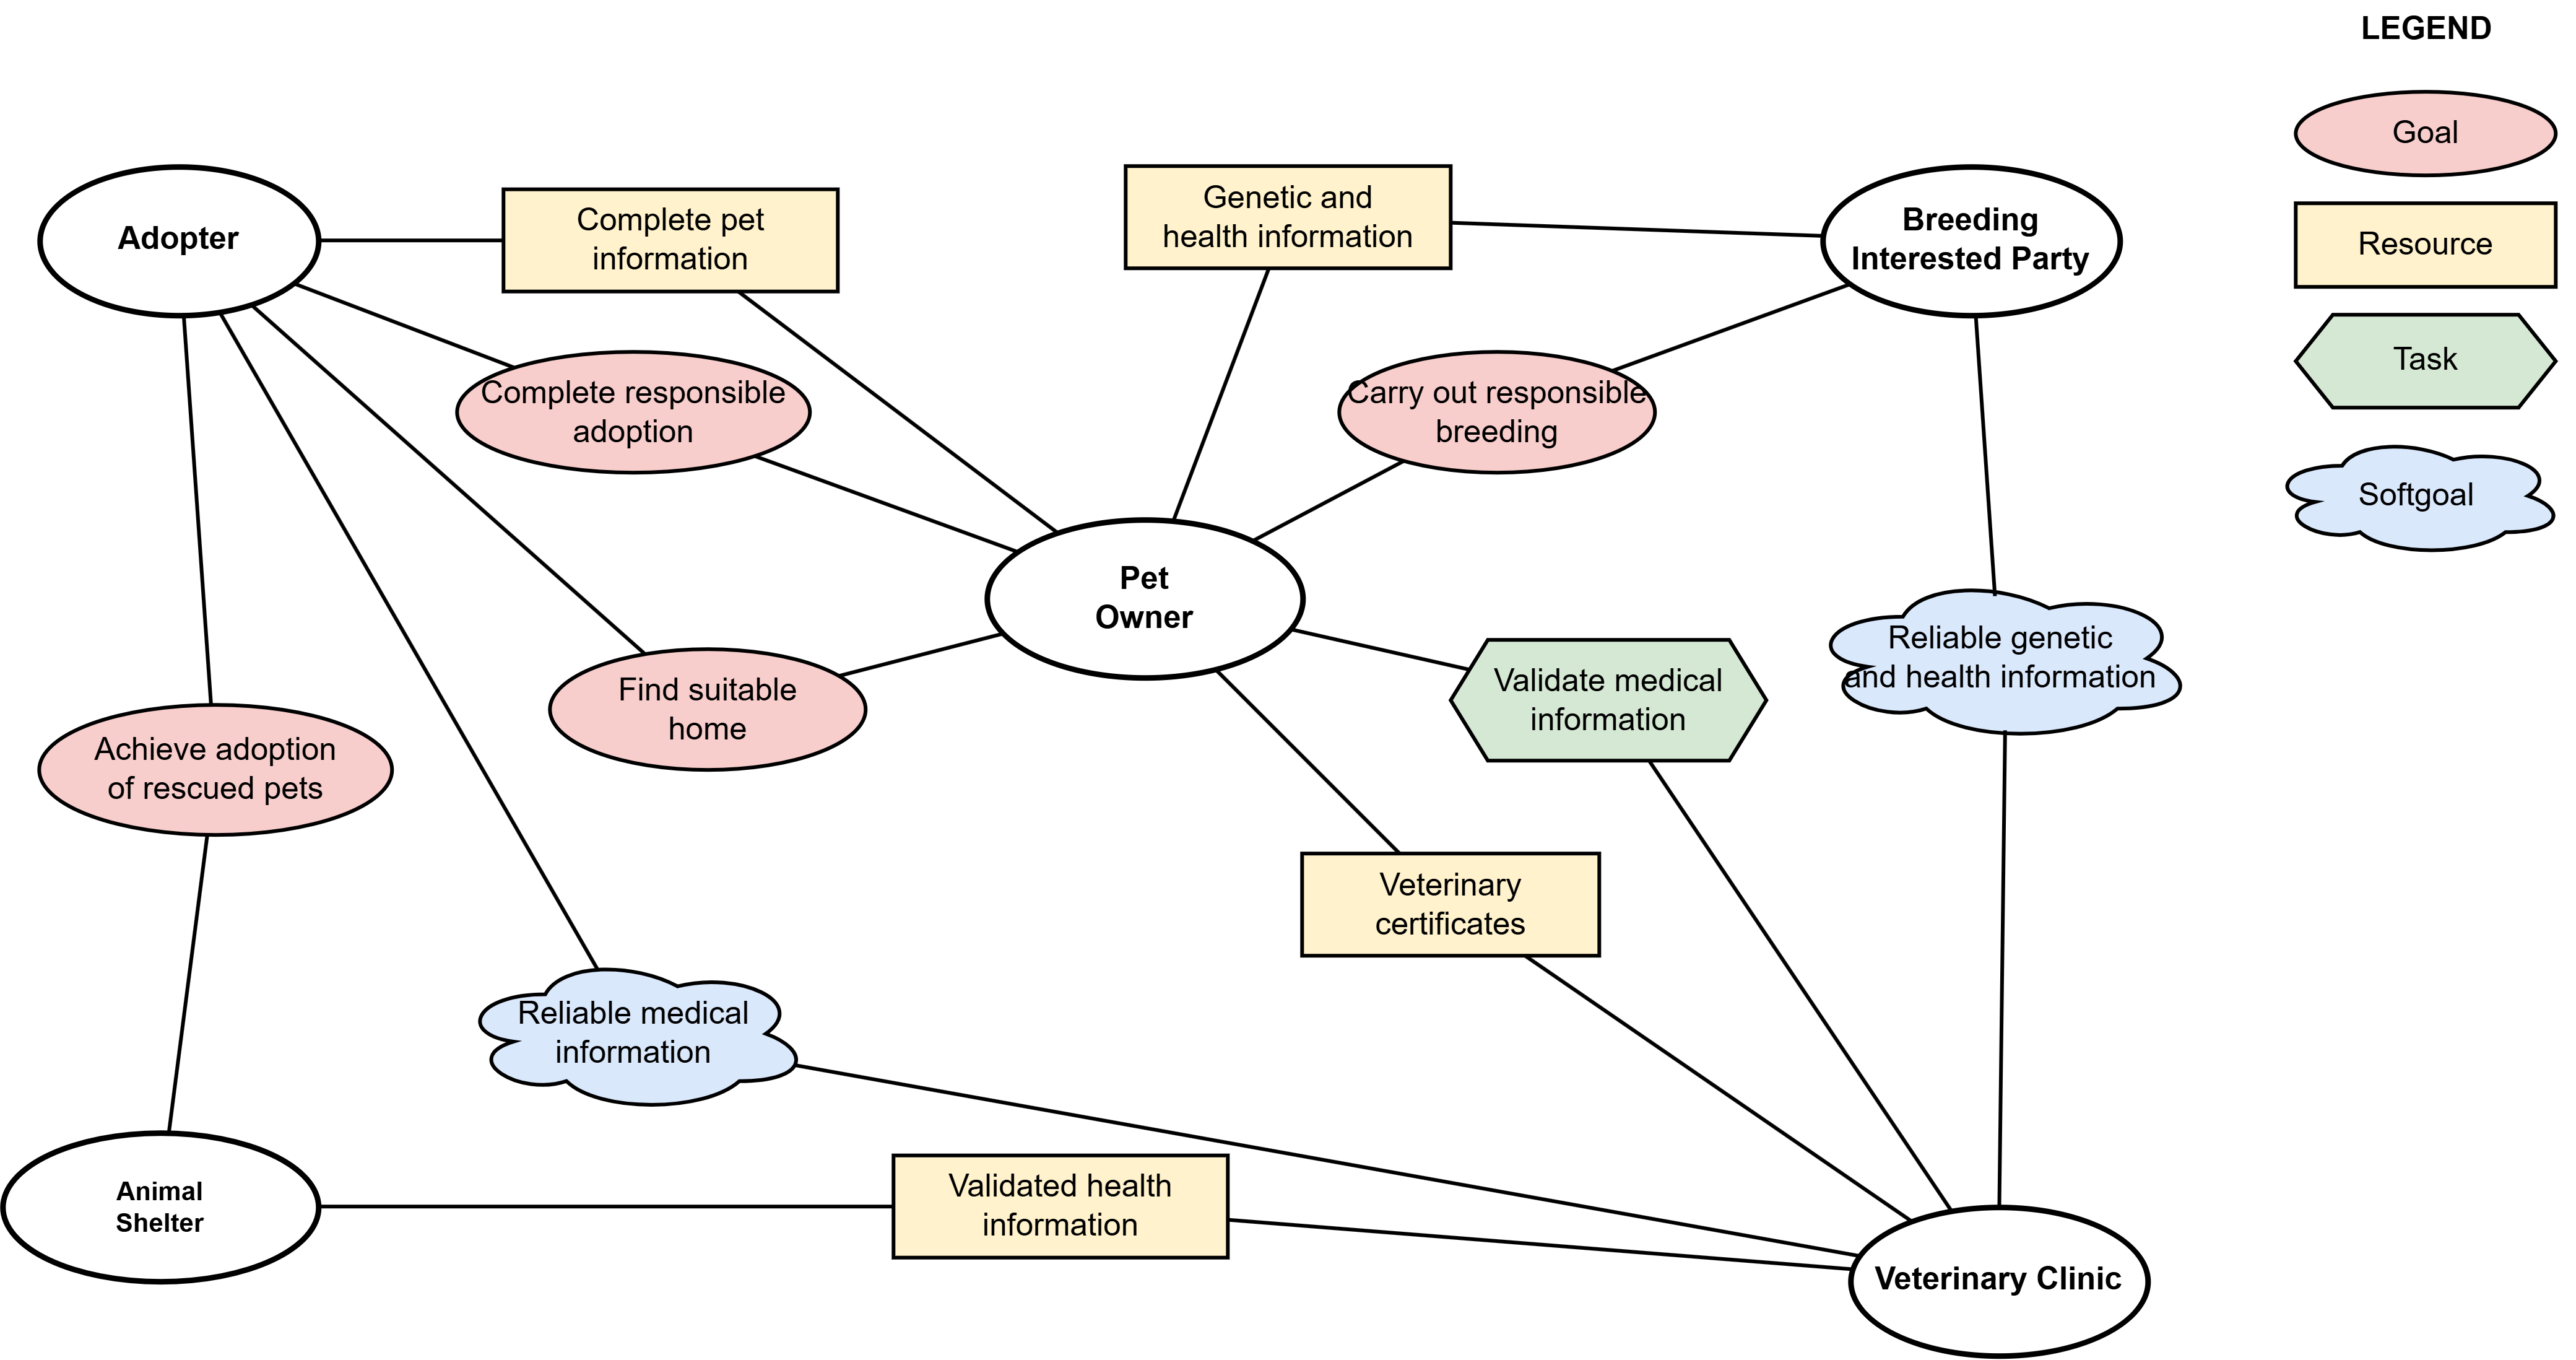
\includegraphics[width=1\textwidth]{figuras/DiagramaDeDependenciaEstrategica_MundiPets.png}
		\caption{Diagrama de dependencias estratégicas (SD) del sistema MundiPets.}
		\label{fig:contexto}
	\end{figure}
	
	Con el fin de representar gráficamente el límite del sistema descrito
	anteriormente, se presenta el diagrama contextual de MundiPets
	(Figura~\ref{fig:diagrama_contexto}), el cual ilustra al sistema como una caja
	única que recibe y envía información hacia los actores externos con los que
	interactúa, sin detallar los procesos internos que lo componen. Este diagrama
	permite visualizar de forma clara el alcance del sistema y los flujos de
	información que cruzan su frontera.
	
	\begin{figure}[H]
		\centering
		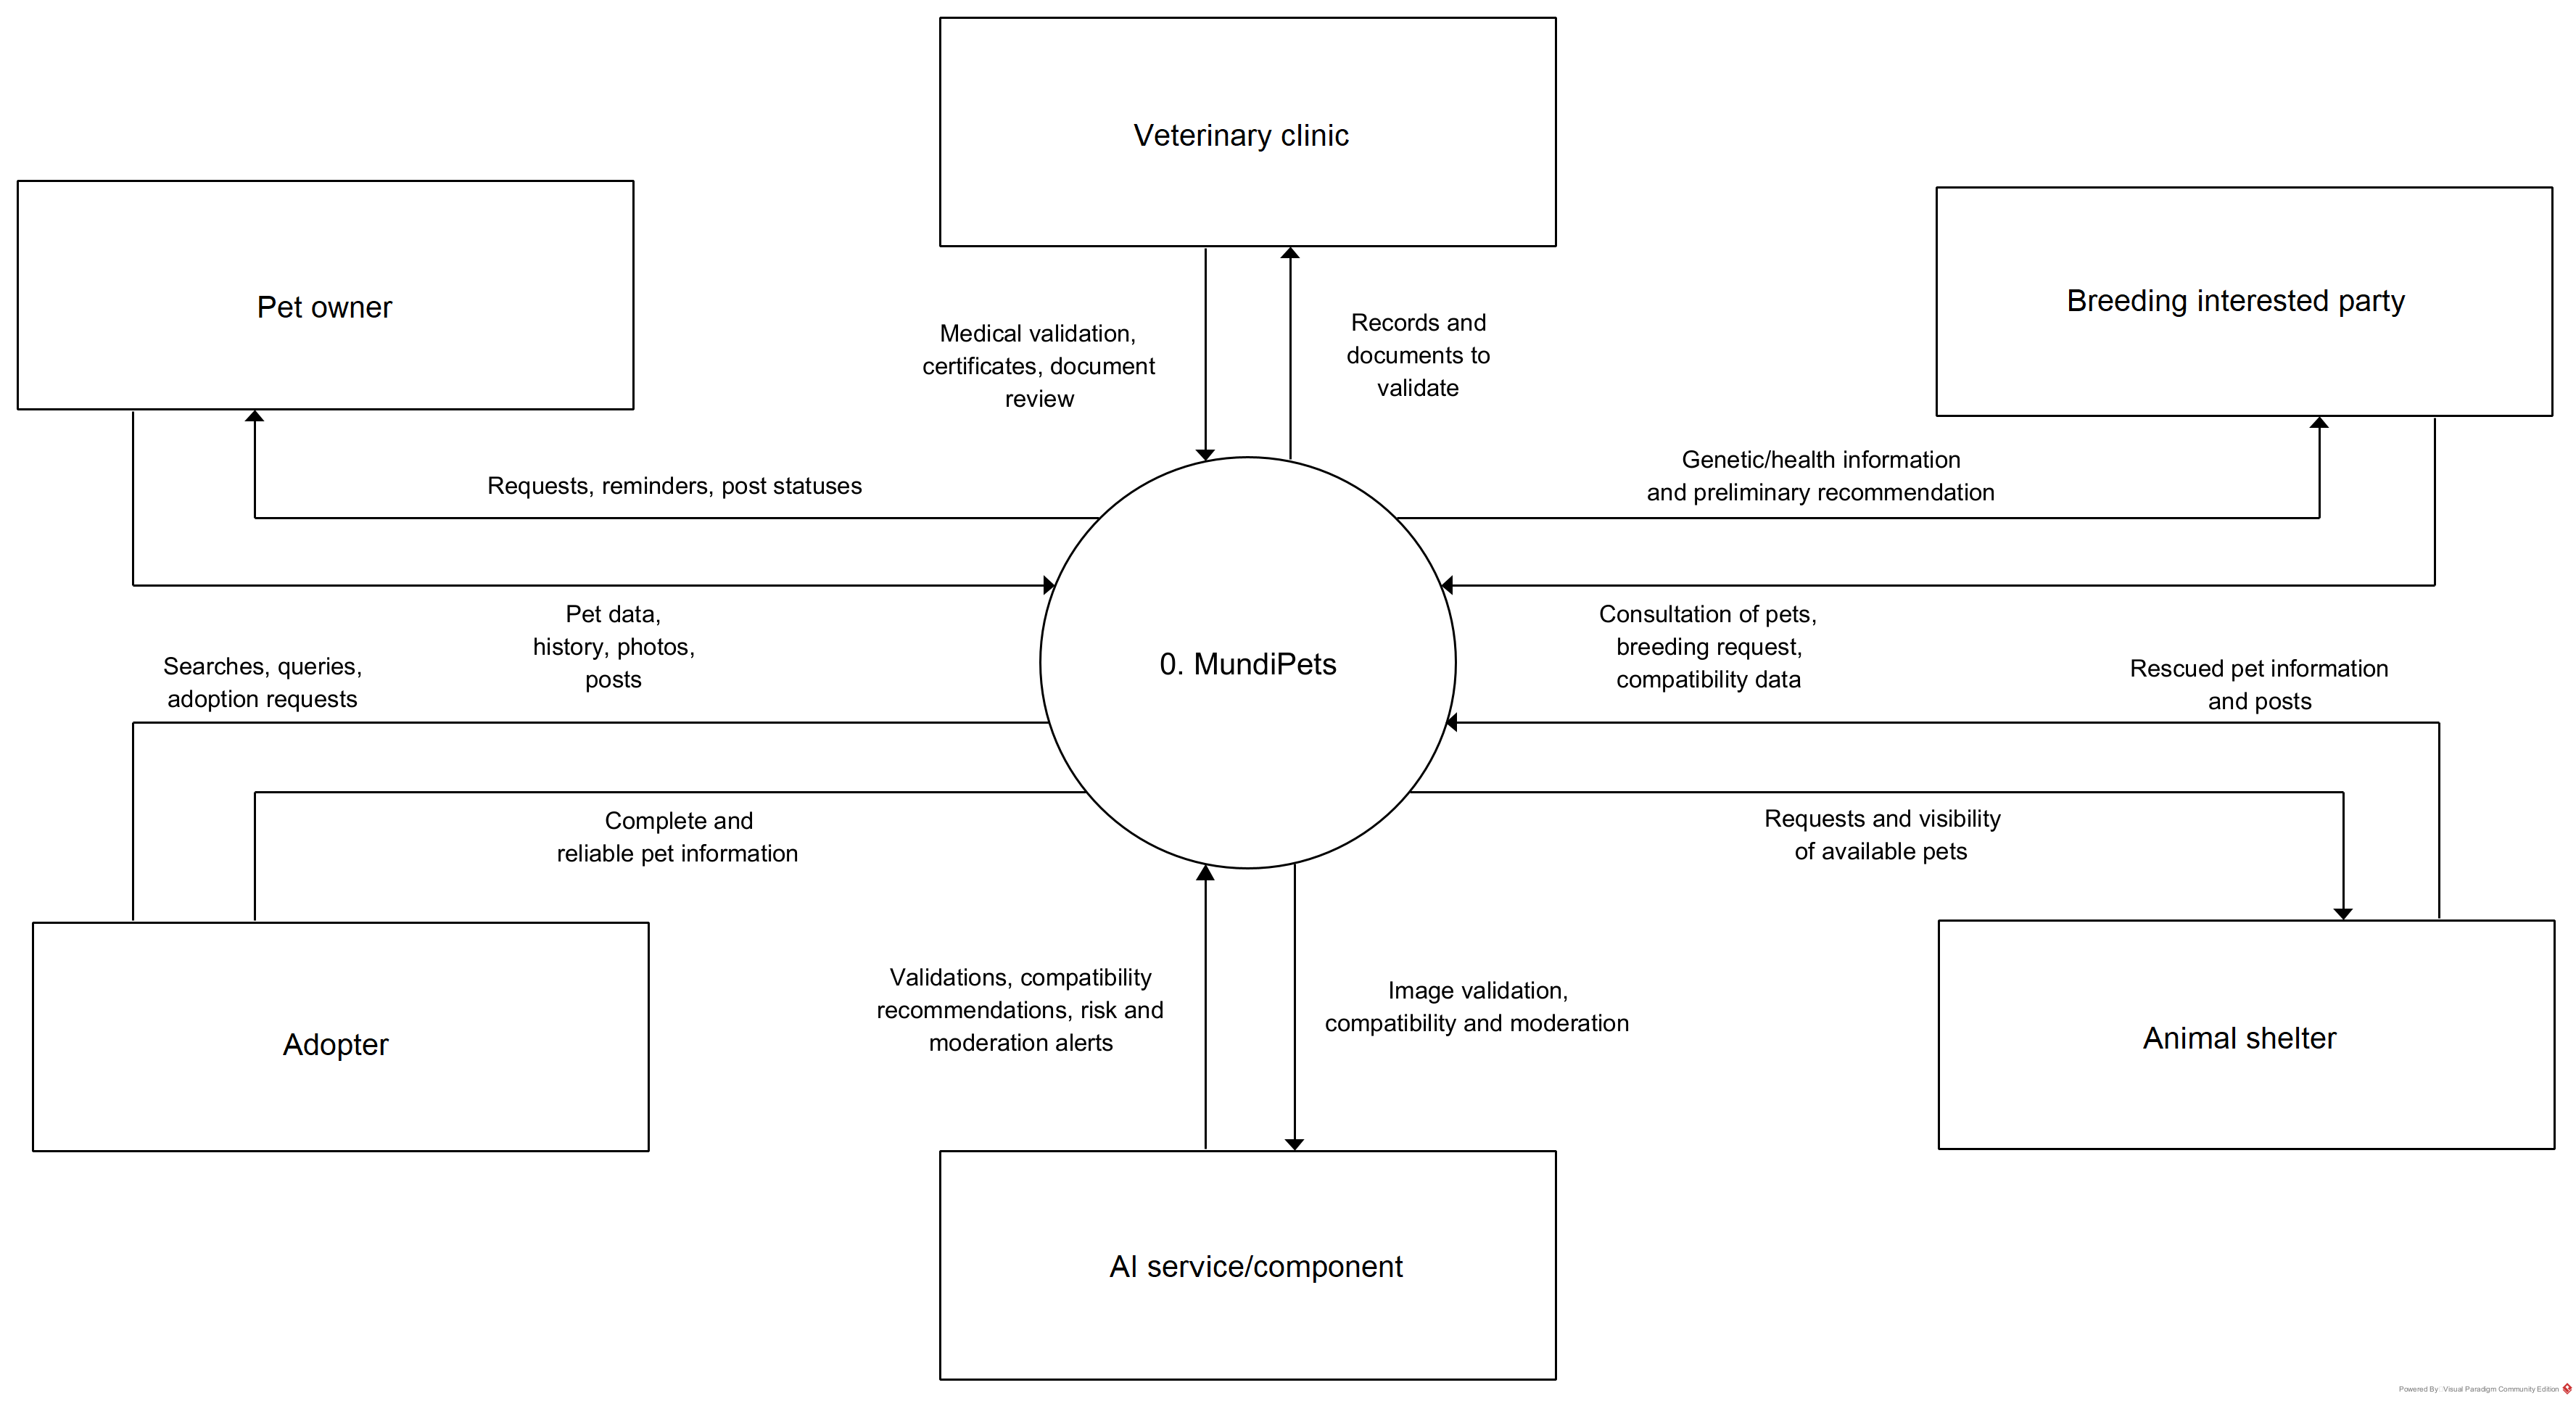
\includegraphics[width=1\textwidth]{figuras/DiagramaContexto_MundiPets.png}
		\caption{Diagrama contextual del sistema MundiPets.}
		\label{fig:diagrama_contexto}
	\end{figure}
	
	\subsection{Funciones del producto}
	\label{sec:funciones}
	
	A continuación se resumen, a alto nivel, las funciones principales que ofrece
	MundiPets, agrupadas por módulo:
	
	\begin{itemize}[leftmargin=*]
		\item \textbf{Gestión de perfiles de mascotas:} permite a los propietarios registrar, editar y publicar la información de sus mascotas (datos generales, historial médico, estado reproductivo).
		\item \textbf{Búsqueda y filtrado:} permite a adoptantes e interesados en cruza buscar mascotas disponibles según criterios como raza, edad, ubicación y propósito (adopción o cruza).
		\item \textbf{Publicación de disponibilidad:} permite a propietarios y refugios publicar mascotas disponibles para adopción o cruza responsable.
		\item \textbf{Validación de información médica:} permite que las veterinarias asociadas verifiquen y certifiquen la información sanitaria y genética cargada en el sistema.
		\item \textbf{Comunicación entre usuarios:} habilita el contacto entre propietario, adoptante e interesado en cruza para coordinar el proceso una vez identificado el interés mutuo.
		\item \textbf{Gestión de mascotas rescatadas:} permite a los refugios de animales publicar y dar seguimiento a mascotas rescatadas en proceso de adopción.
		\item \textbf{Reporte de conversaciones sospechosas:} permite a los usuarios reportar interacciones, mensajes o publicaciones que consideren fraudulentas, irresponsables o inapropiadas, fortaleciendo la seguridad y la confianza dentro de la plataforma.
		\item \textbf{Apoyo basado en inteligencia artificial:} incorpora funcionalidades de soporte orientadas a mejorar la calidad de la información publicada, la seguridad de las interacciones y la responsabilidad en los procesos de adopción y cruza, mediante alertas, recomendaciones preliminares y mecanismos de validación o moderación dentro de la plataforma. Estas funcionalidades no reemplazan la evaluación de profesionales veterinarios ni toman decisiones definitivas sobre la salud o reproducción de las mascotas.
	\end{itemize}
	
	\subsection{Clases y características de usuarios}
	\label{sec:perfiles}
	
	El sistema MundiPets está dirigido a diferentes clases de usuarios que
	participan en los procesos de registro de mascotas, adopción, cruza
	responsable y revisión de información sanitaria. Cada perfil tiene
	necesidades, funciones y niveles de acceso distintos, por lo que es necesario
	identificarlos de forma clara para definir correctamente los requisitos del
	sistema. Esta clasificación permite comprender qué acciones puede realizar
	cada usuario dentro de la plataforma y cómo se relaciona con los demás actores
	del sistema.
	
	\begin{longtable}{|p{2.2cm}|p{3.4cm}|p{3.4cm}|p{3.7cm}|p{1.2cm}|}
		\caption{Clases y características de usuarios del sistema MundiPets.} \label{tab:clases_usuario} \\
		\hline
		\textbf{Clase de usuario} & \textbf{Descripción del perfil} & \textbf{Necesidades principales} & \textbf{Funciones principales} & \textbf{Nivel de acceso} \\
		\hline
		\endfirsthead
		\hline
		\textbf{Clase de usuario} & \textbf{Descripción del perfil} & \textbf{Necesidades principales} & \textbf{Funciones principales} & \textbf{Nivel de acceso} \\
		\hline
		\endhead
		\hline
		\endfoot
		\hline
		\endlastfoot
		
		Propietario de mascota & Persona que registra y administra la información de su mascota dentro de MundiPets. Puede publicar su mascota para adopción o para un proceso de cruza responsable. & Necesita guardar datos completos de su mascota, actualizar su información, publicar su disponibilidad y revisar las solicitudes que recibe. & Crear y editar perfiles de mascotas, subir fotografías, registrar información médica básica, publicar mascotas para adopción o cruza, revisar solicitudes y comunicarse con otros usuarios. & Medio \\ \hline
		
		Adoptante & Persona interesada en encontrar una mascota para adoptar. Necesita información clara antes de tomar una decisión. & Necesita buscar mascotas disponibles, revisar sus datos principales, conocer su estado general y contactar al propietario o refugio. & Explorar mascotas disponibles, usar filtros de búsqueda, revisar perfiles, enviar solicitudes de adopción y comunicarse con propietarios o refugios. & Medio \\ \hline
		
		Interesado en cruza & Persona que busca una mascota compatible para realizar una cruza responsable. Requiere revisar información sanitaria y reproductiva antes de contactar al propietario. & Necesita consultar datos de salud, antecedentes, estado reproductivo y compatibilidad básica de la mascota. & Buscar mascotas disponibles para cruza, consultar perfiles, revisar información sanitaria referencial, enviar solicitudes de cruza y comunicarse con el propietario. & Medio \\ \hline
		
		Refugio de animales & Organización que registra y publica mascotas rescatadas para facilitar su adopción responsable. & Necesita dar visibilidad a las mascotas rescatadas, actualizar su disponibilidad, recibir solicitudes y comunicarse con posibles adoptantes. & Registrar mascotas rescatadas, publicar perfiles para adopción, actualizar estados, revisar solicitudes y comunicarse con adoptantes. & Alto \\ \hline
		
		Veterinaria & Profesional o entidad que revisa documentos e información sanitaria de las mascotas registradas en la plataforma. & Necesita revisar documentos autorizados, verificar información sanitaria referencial y registrar observaciones cuando sea necesario. & Revisar carnés o certificados veterinarios, validar o rechazar información sanitaria referencial y emitir observaciones dentro del sistema. & Alto \\ \hline
	\end{longtable}
	
	\subsection{Mapa de stakeholders}
	\label{sec:stakeholders}
	
	MundiPets involucra a diferentes stakeholders que influyen directa o
	indirectamente en el desarrollo del sistema. Cada uno tiene intereses,
	necesidades y niveles de participación distintos dentro del proyecto.
	Identificarlos permite comprender quiénes usarán la plataforma, quiénes
	aportan información para los requisitos, quiénes validan el contenido
	sanitario y quiénes supervisan el cumplimiento académico y técnico del
	documento ERS/SRS.
	
	\begin{longtable}{|p{1.8cm}|p{2.4cm}|p{1cm}|p{1cm}|p{3.7cm}|p{3.6cm}|}
		\caption{Mapa de stakeholders del sistema MundiPets.} \label{tab:matriz_stakeholders} \\
		\hline
		\textbf{Stakeholder} & \textbf{Interés en el sistema} & \textbf{Poder} & \textbf{Interés} & \textbf{Necesidades y expectativas} & \textbf{Estrategia de gestión} \\
		\hline
		\endfirsthead
		\hline
		\textbf{Stakeholder} & \textbf{Interés en el sistema} & \textbf{Poder} & \textbf{Interés} & \textbf{Necesidades y expectativas} & \textbf{Estrategia de gestión} \\
		\hline
		\endhead
		\hline
		\endfoot
		\hline
		\endlastfoot
		
		Propietario de mascota & Registrar y publicar información de sus mascotas para adopción o cruza responsable. & Medio & Alto & Crear perfiles completos, recibir solicitudes, comunicarse con interesados y mantener actualizada la información de sus mascotas. & Mantener informado y considerar sus necesidades en los requisitos de perfiles, publicaciones y solicitudes. \\ \hline
		
		Adoptante & Buscar mascotas disponibles para adopción con información clara y confiable. & Medio & Alto & Consultar perfiles, revisar datos básicos y sanitarios, aplicar filtros y enviar solicitudes de adopción. & Mantener informado y validar con este perfil las funciones de búsqueda, consulta y solicitud de adopción. \\ \hline
		
		Interesado en cruza & Encontrar mascotas compatibles para un proceso de cruza responsable. & Medio & Alto & Revisar información sanitaria, reproductiva y de comportamiento antes de contactar al propietario. & Mantener informado y considerar sus necesidades en los requisitos de cruza, compatibilidad y comunicación. \\ \hline
		
		Refugio de animales & Publicar mascotas rescatadas y facilitar procesos de adopción responsable. & Alto & Alto & Registrar varias mascotas, actualizar disponibilidad, recibir solicitudes y dar seguimiento a posibles adoptantes. & Gestionar de cerca, porque puede aportar reglas reales sobre adopción, seguimiento y publicación de mascotas rescatadas. \\ \hline
		
		Veterinarios & Revisar información sanitaria y documentos veterinarios registrados en la plataforma. & Alto & Alto & Validar información referencial, revisar carnés o certificados y registrar observaciones técnicas. & Gestionar de cerca mediante consultas sobre vacunas, documentos, salud animal y límites del sistema. \\ \hline
		
		Equipo desarrollador & Analizar, diseñar y documentar los requisitos del sistema MundiPets. & Alto & Alto & Contar con requisitos claros, viables, verificables y trazables para desarrollar el sistema. & Gestionar de cerca, asegurando comunicación constante, control de cambios y revisión técnica. \\ \hline
		
		Docente evaluador & Revisar el cumplimiento académico, metodológico y técnico de la ERS/SRS. & Alto & Alto & Verificar que el documento cumpla la estructura ERS/SRS, los mínimos solicitados y la trazabilidad. & Gestionar de cerca mediante revisión continua del documento, corrección de observaciones y cumplimiento de criterios. \\ \hline
	\end{longtable}
	
	\subsubsection{Matriz poder/interés}
	\label{sec:poder-interes}
	
	\begin{longtable}{|p{3.0cm}|p{1.4cm}|p{1.4cm}|p{3.8cm}|p{4.2cm}|}
		\caption{Matriz poder/interés de stakeholders del sistema MundiPets.} \label{tab:clasificacion_stakeholders} \\
		\hline
		\textbf{Stakeholder} & \textbf{Poder} & \textbf{Interés} & \textbf{Clasificación} & \textbf{Estrategia} \\
		\hline
		\endfirsthead
		\hline
		\textbf{Stakeholder} & \textbf{Poder} & \textbf{Interés} & \textbf{Clasificación} & \textbf{Estrategia} \\
		\hline
		\endhead
		\hline
		\endfoot
		\hline
		\endlastfoot
		
		Refugio de animales & Alto & Alto & Actor clave & Gestionar de cerca \\ \hline
		
		Veterinarios & Alto & Alto & Actor clave técnico & Gestionar de cerca \\ \hline
		
		Equipo desarrollador & Alto & Alto & Actor técnico principal & Gestionar de cerca \\ \hline
		
		Docente evaluador & Alto & Alto & Actor académico clave & Gestionar de cerca \\ \hline
		
		Propietario de mascota & Medio & Alto & Usuario principal & Mantener informado y consultar \\ \hline
		
		Adoptante & Medio & Alto & Usuario principal & Mantener informado y consultar \\ \hline
		
		Interesado en cruza & Medio & Alto & Usuario principal & Mantener informado y consultar \\ \hline
	\end{longtable}
	
	\subsubsection{Conflictos potenciales entre stakeholders}
	\label{sec:conflictos}
	
	\begin{longtable}{|p{2.2cm}|p{2.2cm}|p{2.8cm}|p{3.2cm}|p{3.3cm}|}
		\caption{Conflictos potenciales entre stakeholders del sistema MundiPets.} \label{tab:matriz_conflictos} \\
		\hline
		\textbf{Conflicto potencial} & \textbf{Stakeholders involucrados} & \textbf{Causa del conflicto} & \textbf{Impacto posible en el sistema} & \textbf{Estrategia de gestión} \\
		\hline
		\endfirsthead
		\hline
		\textbf{Conflicto potencial} & \textbf{Stakeholders involucrados} & \textbf{Causa del conflicto} & \textbf{Impacto posible en el sistema} & \textbf{Estrategia de gestión} \\
		\hline
		\endhead
		\hline
		\endfoot
		\hline
		\endlastfoot
		
		Publicación de información incompleta de mascotas & Propietario de mascota, adoptante y refugio. & Algunos usuarios pueden publicar mascotas sin datos suficientes sobre salud, edad, comportamiento o disponibilidad. & Decisiones de adopción o cruza con información incompleta, menor confianza en la plataforma y aumento de solicitudes mal gestionadas. & Definir campos obligatorios, mostrar alertas de perfil incompleto y permitir revisión por el refugio cuando corresponda. \\ \hline
		
		Confianza en la información sanitaria & Propietario de mascota, veterinaria, adoptante e interesado en cruza. & La información médica puede ser registrada por usuarios sin respaldo documental. & Riesgo de que adoptantes o interesados en cruza tomen decisiones con datos poco confiables. & Solicitar documentos veterinarios, permitir validación sanitaria referencial y mostrar el estado de revisión de cada documento. \\ \hline
		
		Privacidad de datos personales y médicos & Propietario, adoptante, interesado en cruza y veterinaria. & Algunos usuarios pueden querer ver más información de la permitida, especialmente datos médicos o de contacto. & Exposición innecesaria de datos sensibles y pérdida de confianza en el sistema. & Definir permisos por rol, limitar datos visibles y permitir acceso solo a la información necesaria según el proceso. \\ \hline
		
		Cruza irresponsable o mal interpretada & Propietario de mascota, interesado en cruza y veterinaria. & Los usuarios pueden interpretar la compatibilidad como autorización definitiva para realizar una cruza. & Riesgos sanitarios, reproductivos o éticos si se realiza una cruza sin revisión profesional. & Aclarar que la plataforma solo ofrece información referencial y recomendar validación veterinaria antes de cualquier decisión. \\ \hline
		
		Diferencias entre necesidades de usuarios y alcance académico & Docente evaluador, equipo desarrollador y usuarios potenciales. & Los usuarios pueden esperar más funciones de las que el proyecto puede desarrollar en esta fase. & Sobrecarga de requisitos, aumento del alcance y dificultad para cumplir la entrega. & Mantener documentado el alcance, clasificar funciones futuras como mejora posterior y priorizar requisitos esenciales. \\ \hline
		
		Validación documental limitada & Veterinaria y propietario de mascota. & La veterinaria puede revisar documentos, pero no reemplaza una consulta médica ni una historia clínica oficial. & Confusión sobre el valor legal o clínico de la validación realizada en la plataforma. & Usar el término ``validación referencial'', no ``certificación clínica'', y aclarar los límites del sistema. \\ \hline
		
		Comunicación inadecuada entre usuarios & Propietario, adoptante e interesado en cruza. & Pueden generarse mensajes fuera de tema, spam, lenguaje ofensivo o acuerdos externos no controlados. & Disminución de la confianza, reportes frecuentes y uso inadecuado de la plataforma. & Incorporar reglas de comunicación, advertencias sobre acuerdos externos y mecanismos básicos para reportar interacciones inadecuadas. \\ \hline
	\end{longtable}
	
	\subsection{Entorno operativo}
	\label{sec:entorno}
	
	MundiPets opera como una aplicación web responsiva, accesible desde
	navegadores de escritorio y dispositivos móviles, sin requerir instalación
	adicional por parte del usuario final.
	
	\textbf{Requisitos del lado del cliente:}
	\begin{itemize}[leftmargin=*]
		\item Navegador web actualizado (Google Chrome, Mozilla Firefox, Microsoft Edge o Safari, en sus versiones recientes).
		\item Conexión a internet estable (mínimo 1 Mbps) para la carga de imágenes y sincronización de datos.
		\item Dispositivo con pantalla táctil o mouse/teclado (smartphone, tablet o computador).
	\end{itemize}
	
	\textbf{Requisitos del lado del servidor:}
	\begin{itemize}[leftmargin=*]
		\item Servidor con soporte para alojamiento web (hosting propio o servicio en la nube).
		\item Base de datos relacional o no relacional según la tecnología seleccionada en la fase de diseño.
		\item Almacenamiento para archivos multimedia (fotografías de mascotas y certificados veterinarios).
	\end{itemize}
	
	Estos requisitos se ajustan al contexto real de uso, en el cual tanto los
	propietarios de mascotas como las veterinarias consultadas acceden
	habitualmente a internet mediante teléfonos inteligentes. Para el Producto
	Mínimo Viable (Sección~\ref{sec:mvp}), el entorno operativo se acota a un
	despliegue local reproducible mediante contenedores, sin necesidad de
	infraestructura de producción.
	
	\subsection{Suposiciones y dependencias}
	\label{sec:suposiciones}
	
	\textbf{Suposiciones:}
	\begin{itemize}[leftmargin=*]
		\item Se asume que los propietarios de mascotas y las veterinarias consultadas cuentan con acceso regular a internet.
		\item Se asume que las veterinarias aliadas estarán dispuestas a validar la información médica cargada por los propietarios, según lo expresado en las entrevistas realizadas.
		\item Se asume que los usuarios proporcionarán información veraz sobre sus mascotas al momento del registro.
		\item Se asume que el volumen inicial de usuarios permitirá operar con una infraestructura básica de hosting durante la primera fase del proyecto.
	\end{itemize}
	
	\textbf{Dependencias externas:}
	\begin{itemize}[leftmargin=*]
		\item El sistema depende de veterinarias externas para la validación y certificación de la información médica y sanitaria de las mascotas (ver diagrama de dependencias, Figura~\ref{fig:contexto}).
		\item El sistema depende de refugios de animales como fuente de información sobre mascotas rescatadas disponibles para adopción.
		\item Podría requerirse la integración con un servicio externo de notificaciones (correo electrónico o mensajería) para alertar a los usuarios sobre nuevas coincidencias o mensajes.
		\item El sistema depende de un proveedor de hosting/almacenamiento en la nube para el despliegue y la persistencia de archivos multimedia.
	\end{itemize}
	
	\subsection{Modelado organizacional en i*}
	\label{sec:istar}
	
	El lenguaje i* \cite{yu1995} modela la intencionalidad de los actores
	organizacionales mediante dos diagramas complementarios. El Diagrama de
	Dependencia Estratégica (SD) muestra qué depende cada actor de los demás sin
	detallar su estructura interna; el Diagrama de Razón Estratégica (SR) abre el
	interior de cada actor y expone sus metas, metas blandas, tareas y recursos.
	
	\subsubsection{Diagrama de Dependencia Estratégica (SD)}
	\label{sec:istar-sd}
	
	La Figura~\ref{fig:contexto} (Sección~\ref{sec:perspectiva}) corresponde al
	Diagrama de Dependencia Estratégica del sistema MundiPets. En él, el
	propietario de mascota depende del sistema para encontrar un adoptante o un
	interesado en cruza adecuado; el adoptante y el interesado en cruza dependen
	del sistema para obtener información confiable sobre las mascotas publicadas;
	la veterinaria actúa como fuente externa de confianza al validar y certificar
	la información médica; y el refugio de animales depende del sistema como
	canal de visibilidad para las mascotas rescatadas. Estas dependencias
	delimitan el conjunto de actores que después se abren en el Diagrama de
	Razón Estratégica.
	
	\subsubsection{Diagrama de Razón Estratégica (SR)}
	\label{sec:istar-sr}
	
	La Figura~\ref{fig:sr} presenta el Diagrama de Razón Estratégica para los tres
	actores principales del sistema: la Veterinaria, el Propietario de mascota y
	el Adoptante/Interesado en cruza.
	
	\begin{figure}[H]
		\centering
		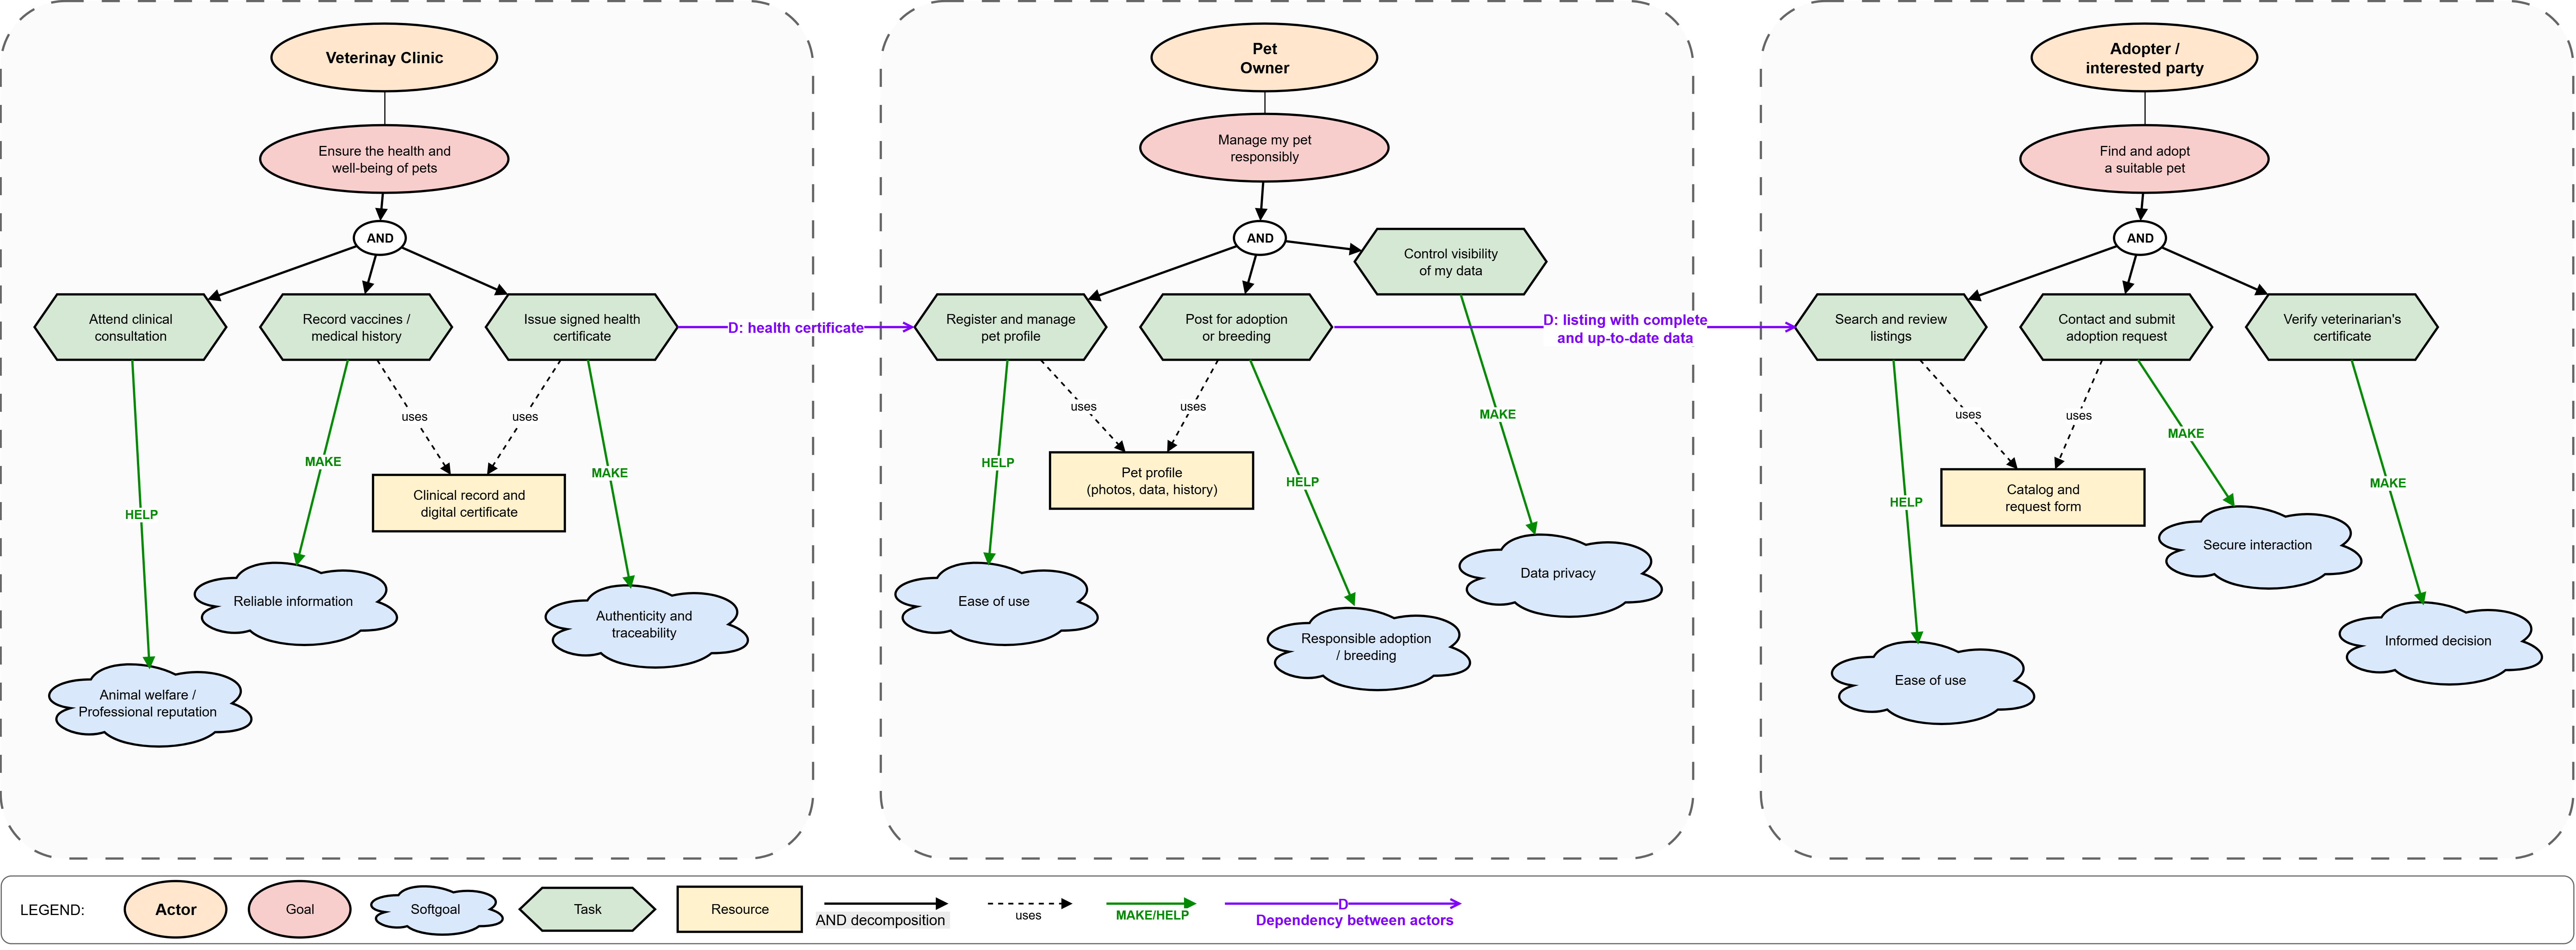
\includegraphics[width=1\textwidth]{figuras/DiagramaDeRazonEstrategica_MundiPets.png}
		\caption{Diagrama de Razón Estratégica (SR) del sistema MundiPets.}
		\label{fig:sr}
	\end{figure}
	
	Para el actor \textbf{Veterinaria}, la meta \emph{garantizar la salud y el
		bienestar de las mascotas} se descompone (mediante descomposición AND) en tres
	tareas: atender la consulta clínica, registrar vacunas e historial médico, y
	emitir el certificado sanitario firmado. Las dos últimas tareas producen los
	recursos \emph{registro clínico y certificado digital}, que a su vez alimentan
	la dependencia de tipo recurso \enquote{certificado de salud} hacia el actor
	Propietario de mascota. Estas tareas contribuyen positivamente a las metas
	blandas \emph{bienestar animal / reputación profesional},
	\emph{información confiable} y \emph{autenticidad y trazabilidad}, conectando
	directamente con RNF-05 (integridad de la información médica) y con el
	requisito legal de minimización de datos sanitarios.
	
	Para el actor \textbf{Propietario de mascota}, la meta \emph{gestionar mi
		mascota de forma responsable} se descompone en las tareas registrar y
	administrar el perfil de la mascota, publicar en adopción o cruza, y
	controlar la visibilidad de mis datos. Las dos primeras tareas usan el
	recurso compartido \emph{perfil de mascota (fotos, datos, historial)} y
	contribuyen a las metas blandas \emph{facilidad de uso} y
	\emph{adopción/cruza responsable}; la tarea de control de visibilidad
	contribuye a la meta blanda \emph{privacidad de los datos}, y la publicación
	del perfil alimenta la dependencia de tipo recurso \enquote{publicación con
		datos completos y actualizados} hacia el actor Adoptante/Interesado en cruza.
	Estas metas blandas se conectan con RNF-01 (protección de la información) y
	RNF-04 (facilidad de uso de la plataforma).
	
	Para el actor \textbf{Adoptante/Interesado en cruza}, la meta \emph{encontrar
		y adoptar una mascota adecuada} se descompone en buscar y revisar
	publicaciones, contactar y enviar una solicitud de adopción o cruza, y
	verificar el certificado de la veterinaria. Las dos primeras tareas usan el
	recurso \emph{catálogo y formulario de solicitud} y contribuyen a las metas
	blandas \emph{facilidad de uso} e \emph{interacción segura}; la verificación
	del certificado contribuye a la meta blanda \emph{decisión informada}, que se
	conecta con RNF-06 (exactitud del componente de inteligencia artificial de
	evaluación de compatibilidad) y con los requisitos de explicabilidad de la
	Sección~\ref{sec:explicabilidad}.
	
	El SR evidencia así cómo las metas blandas de los tres actores --
	\emph{información confiable}, \emph{privacidad de los datos} e
	\emph{interacción segura}, entre otras -- no son aspiraciones abstractas, sino
	que se materializan en los requisitos no funcionales concretos definidos en la
	Sección~\ref{sec:rnf}.
	
	% ############################################################
	%           SECCION 3 -- REQUISITOS ESPECIFICOS COMPLETOS
	% ############################################################
	\section{Requisitos específicos completos}
	\label{sec:requisitos}
	
	\subsection{Interfaces externas}
	\label{sec:interfaces}
	
	Esta sección describe las interfaces a través de las cuales el sistema
	MundiPets interactúa con sus usuarios, con el hardware sobre el que se
	ejecuta y con los servicios de software externos de los que depende,
	siguiendo la estructura recomendada por ISO/IEC/IEEE 29148:2018
	\cite{iso29148}.
	
	\subsubsection{Interfaz de usuario (mockups de alta fidelidad)}
	\label{sec:mockups}
	
	Esta subsección presenta los mockups de alta fidelidad correspondientes a
	las interfaces de usuario que soportan los requisitos funcionales de
	prioridad \emph{Debe tener} del sistema MundiPets. Cada mockup se identifica
	con un código MU-XX, se describe brevemente en función de la interacción que
	representa y se vincula explícitamente con los requisitos funcionales (RF)
	que soporta, en cumplimiento de la trazabilidad exigida por el estándar
	ISO/IEC/IEEE 29148:2018 \cite{iso29148}.
	
	El prototipo navegable completo, elaborado en Figma, se encuentra disponible
	en el siguiente enlace:
	
	\begin{center}
		\small\url{https://www.figma.com/proto/EHp0XoVnL5SNnt8SSFy8AO/Mockups---MundiPets?node-id=20-3}
	\end{center}
	
	\paragraph{MU-01: Crear cuenta}
	
	En la Figura~\ref{fig:mu01} se muestra el mockup de la interfaz de registro y
	verificación de identidad, punto de entrada para los cuatro roles de usuario
	que interactúan con la plataforma (propietario, adoptante, interesado en
	cruza y veterinaria). El formulario solicita los datos de identificación
	básicos y permite adjuntar el documento requerido para la verificación,
	mostrando al usuario el estado de verificación resultante antes de
	habilitarlo para participar en procesos de adopción o cruza.
	
	\textbf{RF asociados:} RF-12.
	
	\begin{figure}[H]
		\centering
		
\includegraphics[width=0.55\textwidth]{{figuras/MU-01_Crear cuenta}.png}
		\caption{Mockup MU-01: Crear cuenta.}
		\label{fig:mu01}
	\end{figure}
	
	\paragraph{MU-02: Registrar mascota}
	
	Este mockup representa el formulario mediante el cual el propietario ingresa
	la información general de una nueva mascota (nombre, especie, raza, sexo,
	edad y estado reproductivo) junto con sus fotografías de identificación. La
	interfaz agrupa los campos obligatorios de forma secuencial y valida su
	completitud antes de habilitar el registro definitivo del perfil dentro de
	la plataforma.
	
	\textbf{RF asociados:} RF-01.
	
	\begin{figure}[H]
		\centering
		
\includegraphics[width=0.62\textwidth]{{figuras/MU-02_Registrar mascota}.png}
		\caption{Mockup MU-02: Registrar mascota.}
		\label{fig:mu02}
	\end{figure}
	
	\paragraph{MU-03: Agenda veterinaria y validación documental}
	
	Este mockup muestra el panel exclusivo para veterinarias, organizado por
	fechas y estados de revisión (pendientes, en revisión, validadas y
	rechazadas). Permite calendarizar la revisión de la documentación sanitaria
	y del carnet de vacunación cargados por los propietarios, y emitir el
	dictamen de validación referencial correspondiente dentro del sistema,
	dejando constancia de la observación técnica en caso de rechazo.
	
	\textbf{RF asociados:} RF-09, RF-14.
	
	\begin{figure}[H]
		\centering
		
\includegraphics[width=0.75\textwidth]{{figuras/MU-03_Agenda Veterinaria y Validación Documental}.png}
		\caption{Mockup MU-03: Agenda veterinaria y validación documental.}
		\label{fig:mu03}
	\end{figure}
	
	\paragraph{MU-04: Feed de publicaciones (búsqueda y filtrado)}
	
	En este mockup se presenta la interfaz que despliega las mascotas
	disponibles en un formato de tarjetas visuales, acompañada de un panel de
	filtros dinámicos (tipo de mascota, estado de interés y ubicación
	aproximada). Permite al adoptante o interesado en cruza refinar la búsqueda
	y seleccionar una tarjeta para acceder al perfil detallado de la mascota o
	iniciar una solicitud.
	
	\textbf{RF asociados:} RF-03, RF-04.
	
	\begin{figure}[H]
		\centering
		
\includegraphics[width=0.75\textwidth]{{figuras/MU-04_Feed de publicaciones (Búsqueda y filtrado)}.png}
		\caption{Mockup MU-04: Feed de publicaciones (búsqueda y filtrado).}
		\label{fig:mu04}
	\end{figure}
	
	\paragraph{MU-05: Solicitud de adopción o cruza}
	
	Este mockup representa el formulario interactivo mediante el cual el usuario
	interesado formaliza su solicitud de adopción o cruza responsable sobre una
	mascota publicada. Incluye la selección del tipo de solicitud, un campo de
	justificación obligatorio, la aceptación explícita de los términos de
	bienestar animal y un canal de mensajería directa que se habilita con el
	propietario una vez enviada la solicitud.
	
	\textbf{RF asociados:} RF-05, RF-07, RF-08.
	
	\begin{figure}[H]
		\centering
		
\includegraphics[width=0.75\textwidth]{{figuras/MU-05_Solicitud de adopción o cruza}.png}
		\caption{Mockup MU-05: Solicitud de adopción o cruza.}
		\label{fig:mu05}
	\end{figure}
	
	\paragraph{MU-06: Perfil de mascota}
	
	En este mockup se muestra la vista de perfil completo de una mascota, que
	centraliza su identidad general, la información sanitaria referencial
	(vacunas, desparasitación y certificado veterinario) y su estado de
	disponibilidad para adopción o cruza. La interfaz distingue el estado de
	vigencia de cada dato sanitario mediante indicadores visuales y ofrece un
	acceso directo para contactar al propietario.
	
	\textbf{RF asociados:} RF-01, RF-02, RF-03, RF-13, RF-16.
	
	\begin{figure}[H]
		\centering
		
\includegraphics[width=0.42\textwidth]{{figuras/MU-06_Perfil de mascota}.png}
		\caption{Mockup MU-06: Perfil de mascota.}
		\label{fig:mu06}
	\end{figure}
	
	\paragraph{MU-07: Evaluación de compatibilidad}
	
	Este mockup representa la interfaz mediante la cual el propietario o el
	interesado en cruza selecciona dos mascotas registradas para obtener una
	recomendación preliminar de compatibilidad. La pantalla presenta ambos
	perfiles de forma comparativa, el resultado generado por el componente de
	inteligencia artificial y su explicación causal asociada, junto con la
	advertencia de que el resultado es orientativo y no sustituye la evaluación
	de un profesional veterinario.
	
	\textbf{RF asociados:} RF-06.
	
	\begin{figure}[H]
		\centering
		
\includegraphics[width=0.68\textwidth]{{figuras/MU-07_Evaluacion de compatibilidad}.png}
		\caption{Mockup MU-07: Evaluación de compatibilidad.}
		\label{fig:mu07}
	\end{figure}
	
	\paragraph{MU-08: Configuración de privacidad de la mascota}
	
	En este mockup se muestra la interfaz mediante la cual el propietario
	administra la visibilidad de la información sensible asociada a su mascota y
	a su propio perfil, tales como la ubicación, los datos de contacto y
	afecciones médicas específicas. Cada categoría de dato sensible cuenta con
	un control independiente de nivel de visibilidad, permitiendo restringir el
	acceso a usuarios no autorizados sin afectar la información obligatoria para
	la validación veterinaria.
	
	\textbf{RF asociados:} RF-11.
	
	\begin{figure}[H]
		\centering
		
\includegraphics[width=0.48\textwidth]{{figuras/MU-08_Configuracion de privacidad de la mascota}.png}
		\caption{Mockup MU-08: Configuración de privacidad de la mascota.}
		\label{fig:mu08}
	\end{figure}
	
	\paragraph{Especificación y trazabilidad de interfaces de usuario}
	
	La Tabla~\ref{tab:trazabilidad_mockups} presenta la matriz de especificación
	y trazabilidad de las interfaces de usuario de MundiPets, detallando los
	códigos de los mockups, las pantallas, los actores, el flujo secuencial de
	acceso y su vinculación directa con los requisitos funcionales (RF) para
	garantizar la trazabilidad del sistema.
	
	{\footnotesize
		\begin{longtable}{@{}L{1.5cm} L{2.0cm} L{2.3cm} L{3.2cm} L{2.0cm} L{2.9cm}@{}}
			\caption{Matriz de especificación y trazabilidad de las interfaces de usuario.}
			\label{tab:trazabilidad_mockups}\\
			\toprule
			\textbf{ID Mockup} & \textbf{Interfaz} & \textbf{Usuario principal} & \textbf{Flujo de navegación} & \textbf{RF vinculados} & \textbf{Justificación} \\
			\midrule
			\endfirsthead
			\multicolumn{6}{@{}l}{\small\itshape (continuación)}\\
			\toprule
			\textbf{ID Mockup} & \textbf{Interfaz} & \textbf{Usuario principal} & \textbf{Flujo de navegación} & \textbf{RF vinculados} & \textbf{Justificación} \\
			\midrule
			\endhead
			\bottomrule
			\endlastfoot
			MU-01 & Crear cuenta & Propietario / Adoptante / Interesado en cruza / Veterinaria & Landing $\rightarrow$ \enquote{Crear cuenta} $\rightarrow$ Formulario de registro $\rightarrow$ Verificación de identidad & RF-12 & Formaliza el registro y la verificación de identidad exigida antes de participar en procesos de adopción o cruza. \\
			\addlinespace
			MU-02 & Registrar mascota & Propietario de mascota & Dashboard $\rightarrow$ Mis Mascotas $\rightarrow$ \enquote{Agregar mascota} $\rightarrow$ Formulario de datos generales & RF-01 & Captura los datos básicos y fotográficos que dan origen al perfil de la mascota dentro de la plataforma. \\
			\addlinespace
			MU-03 & Agenda veterinaria y validación documental & Veterinaria & Dashboard $\rightarrow$ Validaciones $\rightarrow$ Agenda de revisiones $\rightarrow$ Detalle del documento & RF-09, RF-14 & Organiza cronológicamente la revisión de documentos sanitarios y del carnet de vacunación por parte de un profesional autorizado. \\
			\addlinespace
			MU-04 & Feed de publicaciones (búsqueda y filtrado) & Adoptante / Interesado en cruza & Menú principal $\rightarrow$ Explorar Mascotas $\rightarrow$ Filtros dinámicos & RF-03, RF-04 & Presenta el catálogo de mascotas disponibles mediante tarjetas visuales y filtros de búsqueda combinables. \\
			\addlinespace
			MU-05 & Solicitud de adopción o cruza & Adoptante / Interesado en cruza & Feed de publicaciones $\rightarrow$ Tarjeta de mascota $\rightarrow$ Botón \enquote{Solicitar} $\rightarrow$ Formulario de solicitud & RF-05, RF-07, RF-08 & Formaliza el interés sobre una mascota, recopila la justificación del solicitante y abre el canal de mensajería con el propietario. \\
			\addlinespace
			MU-06 & Perfil de mascota & Propietario / Adoptante / Interesado en cruza & Feed de publicaciones $\rightarrow$ Tarjeta de mascota $\rightarrow$ Ver perfil completo & RF-01, RF-02, RF-03, RF-13, RF-16 & Centraliza la identidad, el historial médico referencial y los antecedentes genéticos de la mascota para sustentar decisiones de adopción o cruza. \\
			\addlinespace
			MU-07 & Evaluación de compatibilidad & Propietario de mascota / Interesado en cruza & Perfil de mascota $\rightarrow$ \enquote{Evaluar compatibilidad} $\rightarrow$ Selección de segunda mascota $\rightarrow$ Resultado & RF-06 & Presenta el resultado comparativo generado por el componente de inteligencia artificial junto con su explicación causal, sin sustituir la evaluación veterinaria. \\
			\addlinespace
			MU-08 & Configuración de privacidad de la mascota & Propietario de mascota & Dashboard $\rightarrow$ Configuración $\rightarrow$ Privacidad de mi mascota & RF-11 & Permite al propietario definir qué información sensible (ubicación, contacto, afecciones específicas) es visible para otros usuarios. \\
		\end{longtable}
	}
	
	Los ocho mockups cubren la totalidad de los requisitos funcionales de
	prioridad \emph{Must} y los casos de uso especificados en la
	Sección~\ref{sec:cu-detallado}, de modo que cada caso de uso dispone de al
	menos una pantalla asociada. Los requisitos funcionales de prioridad
	\emph{Should} y \emph{Could} (RF-10, RF-15, RF-17 a RF-25) se apoyan sobre
	las mismas pantallas mediante secciones secundarias o se difieren a
	iteraciones posteriores del prototipo, conforme al alcance del Producto
	Mínimo Viable definido en la Sección~\ref{sec:mvp-alcance}.
	
	\subsubsection{Interfaz de hardware}
	\label{sec:interfaz-hardware}
	
	MundiPets es una aplicación web responsiva que no requiere hardware
	especializado ni controladores propietarios; toda la interacción con los
	dispositivos se realiza a través de las API estándar expuestas por el
	navegador, en coherencia con el entorno operativo descrito en la
	Sección~\ref{sec:entorno} y con la portabilidad exigida por RNF-11. Las
	interfaces de hardware relevantes son las siguientes:
	
	\begin{itemize}[leftmargin=*]
		\item \textbf{Cámara y almacenamiento local del dispositivo.} Se accede
		mediante el selector de archivos y la API \texttt{MediaDevices} del
		navegador para capturar o adjuntar las fotografías de la mascota (RF-01)
		y los documentos veterinarios digitalizados (RF-14). El sistema no accede
		al hardware fuera de la acción explícita del usuario.
		\item \textbf{Servicios de geolocalización.} Se emplea la
		\texttt{Geolocation API} del navegador, previa autorización del usuario,
		para derivar la zona aproximada de la mascota. La ubicación exacta nunca
		se almacena ni se muestra, conforme a RNF-16 y a la configuración de
		privacidad de RF-11.
		\item \textbf{Pantalla y dispositivos de entrada.} La interfaz se adapta a
		pantallas táctiles y a la combinación de teclado y ratón, con un diseño
		responsivo verificable en resoluciones de teléfono inteligente, tableta y
		computador de escritorio (RNF-04, RNF-11).
		\item \textbf{Conectividad de red.} Se requiere una conexión a internet
		estable de al menos 1\,Mbps para la carga de imágenes y la sincronización
		de datos; el sistema no define ninguna interfaz de red propietaria.
		\item \textbf{Infraestructura del lado del servidor.} No se impone hardware
		específico: el despliegue se realiza sobre servidores virtualizados o
		contenedores en un proveedor de nube, de acuerdo con la escalabilidad
		horizontal exigida por RNF-12.
	\end{itemize}
	
	\subsubsection{Interfaz de software}
	\label{sec:interfaz-software}
	
	El sistema se comunica con componentes y servicios externos a través de
	interfaces de software bien delimitadas. La Tabla~\ref{tab:interfaz_software}
	resume cada interfaz, su propósito, el mecanismo de intercambio previsto y
	los requisitos que la sustentan.
	
	{\footnotesize
		\begin{longtable}{@{}L{3.2cm} L{4.5cm} L{3.4cm} L{3.4cm}@{}}
			\caption{Interfaces de software del sistema MundiPets.}
			\label{tab:interfaz_software}\\
			\toprule
			\textbf{Interfaz externa} & \textbf{Propósito} & \textbf{Mecanismo de intercambio} & \textbf{Requisitos asociados} \\
			\midrule
			\endfirsthead
			\multicolumn{4}{@{}l}{\small\itshape (continuación)}\\
			\toprule
			\textbf{Interfaz externa} & \textbf{Propósito} & \textbf{Mecanismo de intercambio} & \textbf{Requisitos asociados} \\
			\midrule
			\endhead
			\bottomrule
			\endlastfoot
			Navegador web del cliente & Renderizado de la interfaz de usuario y consumo de los servicios de la aplicación & HTTPS sobre HTML5, CSS3 y JavaScript; respuestas en JSON & RNF-04, RNF-11 \\
			\addlinespace
			Componente de evaluación de compatibilidad (IA) & Generar el resultado orientativo de cruza y su explicación causal & API interna REST/JSON expuesta por el módulo de IA (Sección~\ref{sec:componentes}) & RF-06, RNF-06, RNF-13, RD-01 \\
			\addlinespace
			Componente de validación de imágenes (IA) & Verificar que la fotografía corresponde a una mascota y es apropiada & API interna REST/JSON & RF-17, RNF-07, RNF-14 \\
			\addlinespace
			Componente de moderación de mensajes (IA) & Clasificar el contenido de los mensajes antes de su entrega & API interna REST/JSON & RF-07, RNF-15 \\
			\addlinespace
			WhatsApp Business API & Envío de recordatorios de controles preventivos y notificaciones & API REST del proveedor sobre HTTPS, con canal de respaldo \emph{in-app} & RF-10, RNF-09, RD-08 \\
			\addlinespace
			Servicio de correo electrónico & Confirmación de cuenta, recuperación de contraseña y avisos del sistema & SMTP o API del proveedor sobre canal cifrado & RF-12, RNF-09 \\
			\addlinespace
			Sistema gestor de base de datos & Persistencia de la información transaccional del sistema & Conexión cifrada mediante el controlador del SGBD seleccionado & RNF-01, RNF-05, RNF-12 \\
			\addlinespace
			Almacenamiento de archivos multimedia & Persistencia de fotografías de mascotas y documentos veterinarios & API de almacenamiento de objetos sobre HTTPS, con URL firmadas de acceso temporal & RF-01, RF-14, RNF-01, RD-04 \\
		\end{longtable}
	}
	
	Todas las comunicaciones con servicios externos se realizan sobre canales
	cifrados y transmiten únicamente los datos estrictamente necesarios para la
	operación solicitada, en cumplimiento del principio de minimización de datos
	de la LOPDP recogido en la Sección~\ref{sec:legales} y de la restricción de
	diseño RD-04. Cuando un servicio externo no se encuentre disponible, el
	sistema degrada la funcionalidad de forma controlada --- por ejemplo,
	sustituyendo la notificación por mensajería con una notificación interna ---
	sin interrumpir el resto de la operación, según lo previsto en RD-08.
	
	% ------------------------------------------------------------
	\subsection{Requisitos funcionales}
	\label{sec:rf}
	
	Los requisitos funcionales se especifican con los ocho atributos exigidos por la
	plantilla de la asignatura, aplicando las recomendaciones de redacción de
	ISO/IEC/IEEE 29148:2018 \cite{iso29148}.
	
	\subsubsection{RF-01 --- Registrar mascota}
	
	\begin{atributos}{RF-01}{RF-01 --- Registrar mascota.}
		Identificador & RF-01 \\
		Nombre & Registrar mascota \\
		Descripción & El sistema deberá permitir al propietario registrar una mascota ingresando su información general, incluyendo nombre, especie, raza, sexo, edad, estado reproductivo y fotografías para su identificación dentro de la plataforma. \\
		Actor & Propietario de mascota \\
		Origen (ID de evidencia) & EV-02, EV-03, EV-05, EV-06, EV-07, EV-08 \\
		Entradas & Nombre, especie, raza, sexo, edad, estado reproductivo, fotografías, descripción. \\
		Salidas & Perfil de mascota registrado correctamente. \\
		Precondiciones & El propietario debe estar autenticado en el sistema. \\
		Postcondiciones & La mascota queda almacenada y disponible para futuras consultas, adopciones o procesos de cruza. \\
		Prioridad (MoSCoW) & Must \\
		Criterio de verificación & Registrar una mascota con datos válidos y comprobar que el perfil queda almacenado y puede consultarse posteriormente. \\
	\end{atributos}
	
	\subsubsection{RF-02 --- Gestionar historial médico de la mascota}
	
	\begin{atributos}{RF-02}{RF-02 --- Gestionar historial médico de la mascota.}
		Identificador & RF-02 \\
		Nombre & Gestionar historial médico de la mascota \\
		Descripción & El sistema deberá permitir registrar y actualizar el historial médico de una mascota, incluyendo vacunas (con su cepa/marca y profesional aplicador), desparasitaciones, enfermedades, alergias, cirugías, tratamientos y controles veterinarios. \\
		Actor & Propietario de mascota, Veterinaria \\
		Origen (ID de evidencia) & EV-01, EV-02, EV-03, EV-04, EV-05, EV-06, EV-07, EV-15, EV-16 \\
		Entradas & Vacunas (cepa, aplicador), desparasitaciones, enfermedades, alergias, cirugías, tratamientos, controles médicos, observaciones. \\
		Salidas & Historial médico actualizado. \\
		Precondiciones & La mascota debe estar registrada en el sistema. \\
		Postcondiciones & El historial médico queda actualizado y disponible para usuarios autorizados. \\
		Prioridad (MoSCoW) & Must \\
		Criterio de verificación & Registrar nuevos antecedentes médicos y verificar que aparecen correctamente dentro del historial clínico de la mascota. \\
	\end{atributos}
	
	\subsubsection{RF-03 --- Consultar perfil completo de una mascota}
	
	\begin{atributos}{RF-03}{RF-03 --- Consultar perfil completo de una mascota.}
		Identificador & RF-03 \\
		Nombre & Consultar perfil completo de una mascota \\
		Descripción & El sistema deberá permitir visualizar el perfil completo de una mascota mostrando su información general, historial médico autorizado, fotografías, comportamiento, vacunas, edad, raza para procesos de adopción o cruza. \\
		Actor & Propietario de mascota, Adoptante, Interesado en cruza \\
		Origen (ID de evidencia) & EV-02, EV-04, EV-05, EV-06, EV-07, EV-14 \\
		Entradas & Identificador de la mascota. \\
		Salidas & Perfil completo de la mascota. \\
		Precondiciones & La mascota debe existir y el usuario debe tener permisos para visualizar la información correspondiente. \\
		Postcondiciones & El usuario obtiene la información necesaria para tomar decisiones sobre adopción o cruza. \\
		Prioridad (MoSCoW) & Must \\
		Criterio de verificación & Consultar una mascota registrada y comprobar que se muestra toda la información autorizada. \\
	\end{atributos}
	
	\subsubsection{RF-04 --- Buscar y filtrar mascotas}
	
	\begin{atributos}{RF-04}{RF-04 --- Buscar y filtrar mascotas.}
		Identificador & RF-04 \\
		Nombre & Buscar y filtrar mascotas \\
		Descripción & El sistema deberá permitir buscar mascotas aplicando filtros como especie, raza, edad, ubicación, estado de salud, tamaño, temperamento y disponibilidad para adopción o cruza. \\
		Actor & Adoptante, Interesado en cruza \\
		Origen (ID de evidencia) & EV-07, EV-08 \\
		Entradas & Criterios de búsqueda y filtros seleccionados. \\
		Salidas & Lista de mascotas que cumplen los criterios establecidos. \\
		Precondiciones & Deben existir mascotas registradas en la plataforma. \\
		Postcondiciones & Se muestran únicamente las mascotas que cumplen los filtros aplicados. \\
		Prioridad (MoSCoW) & Should \\
		Criterio de verificación & Aplicar diferentes filtros, incluidos tamaño y temperamento, y comprobar que los resultados corresponden con los criterios seleccionados. \\
	\end{atributos}
	
	\subsubsection{RF-05 --- Gestionar solicitudes de adopción}
	
	\begin{atributos}{RF-05}{RF-05 --- Gestionar solicitudes de adopción.}
		Identificador & RF-05 \\
		Nombre & Gestionar solicitudes de adopción \\
		Descripción & El sistema deberá permitir que un usuario interesado envíe solicitudes de adopción, incluyendo su fotografía de perfil, y que el propietario pueda aceptarlas o rechazarlas después de revisar la información del solicitante. \\
		Actor & Adoptante, Propietario de mascota \\
		Origen (ID de evidencia) & EV-01, EV-02, EV-03, EV-05, EV-06, EV-08 \\
		Entradas & Solicitud de adopción, información y fotografía del solicitante. \\
		Salidas & Solicitud registrada y estado de aceptación o rechazo. \\
		Precondiciones & La mascota debe estar disponible para adopción. \\
		Postcondiciones & La solicitud queda registrada con su estado correspondiente. \\
		Prioridad (MoSCoW) & Must \\
		Criterio de verificación & Registrar una solicitud y comprobar que el propietario puede visualizar el perfil del solicitante y gestionarla correctamente. \\
	\end{atributos}
	
	\subsubsection{RF-06 --- Evaluar compatibilidad entre mascotas para cruza}
	
	\begin{atributos}{RF-06}{RF-06 --- Evaluar compatibilidad entre mascotas para cruza.}
		Identificador & RF-06 \\
		Nombre & Evaluar compatibilidad entre mascotas para cruza \\
		Descripción & El sistema deberá evaluar la compatibilidad entre dos mascotas registradas para procesos de cruza, considerando su raza, edad, estado de salud, antecedentes genéticos, parentesco, comportamiento e historial médico. \\
		Actor & Propietario de mascota, Interesado en cruza \\
		Origen (ID de evidencia) & EV-01 a EV-08, EV-11, EV-13, EV-14, EV-15, EV-16 \\
		Entradas & Selección de dos mascotas registradas. \\
		Salidas & Información comparativa para evaluar la compatibilidad, junto con una advertencia de que el resultado es orientativo y no sustituye la evaluación de un veterinario. \\
		Precondiciones & Ambas mascotas deben encontrarse registradas. \\
		Postcondiciones & El usuario dispone de información suficiente para decidir si continúa con el proceso de cruza. \\
		Prioridad (MoSCoW) & Must \\
		Criterio de verificación & Seleccionar dos mascotas y comprobar que el sistema presenta la información comparativa junto con la advertencia orientativa. \\
	\end{atributos}
	
	\subsubsection{RF-07 --- Sistema de mensajería entre usuarios}
	
	\begin{atributos}{RF-07}{RF-07 --- Sistema de mensajería entre usuarios.}
		Identificador & RF-07 \\
		Nombre & Sistema de mensajería entre usuarios \\
		Descripción & El sistema deberá permitir la comunicación entre propietarios e interesados mediante mensajes para coordinar procesos de adopción y cruza. \\
		Actor & Propietario de mascota, Adoptante, Interesado en cruza \\
		Origen (ID de evidencia) & EV-02, EV-07, EV-08 \\
		Entradas & Mensaje enviado por un usuario. \\
		Salidas & Conversación registrada entre los usuarios. \\
		Precondiciones & Ambos usuarios deben encontrarse registrados. \\
		Postcondiciones & El mensaje queda almacenado y disponible para ambos participantes. \\
		Prioridad (MoSCoW) & Could \\
		Criterio de verificación & Enviar un mensaje entre dos usuarios y verificar que ambos puedan visualizarlo. \\
	\end{atributos}
	
	\subsubsection{RF-08 --- Gestionar solicitudes de cruza}
	
	\begin{atributos}{RF-08}{RF-08 --- Gestionar solicitudes de cruza.}
		Identificador & RF-08 \\
		Nombre & Gestionar solicitudes de cruza \\
		Descripción & El sistema deberá permitir que los propietarios soliciten procesos de cruza entre mascotas y que el propietario de la otra mascota pueda aceptar o rechazar la solicitud con base en la información disponible. \\
		Actor & Propietario de mascota, Interesado en cruza \\
		Origen (ID de evidencia) & EV-01, EV-02, EV-03, EV-05, EV-06, EV-07 \\
		Entradas & Solicitud de cruza, identificación de ambas mascotas. \\
		Salidas & Solicitud registrada con estado pendiente, aceptada o rechazada. \\
		Precondiciones & Ambas mascotas deben estar registradas y disponibles para cruza. \\
		Postcondiciones & La solicitud queda almacenada y actualizada con el estado correspondiente. \\
		Prioridad (MoSCoW) & Must \\
		Criterio de verificación & Registrar una solicitud de cruza y verificar que el propietario receptor pueda aceptarla o rechazarla correctamente. \\
	\end{atributos}
	
	\subsubsection{RF-09 --- Validar la información médica de una mascota}
	
	\begin{atributos}{RF-09}{RF-09 --- Validar la información médica de una mascota.}
		Identificador & RF-09 \\
		Nombre & Validar la información médica de una mascota \\
		Descripción & El sistema deberá permitir que una veterinaria autorizada valide la información médica registrada de una mascota, indicando que los datos han sido verificados por un profesional. \\
		Actor & Veterinaria \\
		Origen (ID de evidencia) & EV-03, EV-05, EV-07, EV-15, EV-16 \\
		Entradas & Historial médico, carnet de vacunación, controles veterinarios y documentos clínicos. \\
		Salidas & Información médica validada con su respectiva identificación de verificación. \\
		Precondiciones & La mascota debe encontrarse registrada y disponer de información médica cargada en el sistema. \\
		Postcondiciones & La información médica queda marcada como validada por una veterinaria autorizada. \\
		Prioridad (MoSCoW) & Must \\
		Criterio de verificación & Validar el historial médico de una mascota y comprobar que el sistema muestre el estado de información validada. \\
	\end{atributos}
	
	\subsubsection{RF-10 --- Gestionar recordatorios de controles preventivos}
	
	\begin{atributos}{RF-10}{RF-10 --- Gestionar recordatorios de controles preventivos.}
		Identificador & RF-10 \\
		Nombre & Gestionar recordatorios de controles preventivos \\
		Descripción & El sistema deberá generar recordatorios por notificación en la aplicación y WhatsApp para informar al propietario sobre próximas vacunas, desparasitaciones y controles veterinarios, enviándolos con una semana y un día de anticipación. \\
		Actor & Propietario de mascota \\
		Origen (ID de evidencia) & EV-02, EV-04, EV-06, EV-11 \\
		Entradas & Fechas de vacunas, controles veterinarios y desparasitaciones. \\
		Salidas & Notificaciones o recordatorios generados por el sistema en los dos momentos definidos. \\
		Precondiciones & Deben existir fechas registradas para los controles preventivos de la mascota. \\
		Postcondiciones & El propietario recibe el recordatorio correspondiente antes de la fecha programada. \\
		Prioridad (MoSCoW) & Should \\
		Criterio de verificación & Registrar una fecha de vacunación próxima y verificar que el sistema genere el recordatorio una semana y un día antes. \\
	\end{atributos}
	
	\subsubsection{RF-11 --- Administrar la privacidad de la información}
	
	\begin{atributos}{RF-11}{RF-11 --- Administrar la privacidad de la información.}
		Identificador & RF-11 \\
		Nombre & Administrar la privacidad de la información \\
		Descripción & El sistema deberá permitir que el propietario determine qué información de su mascota y de su perfil podrá ser visualizada por otros usuarios, protegiendo los datos considerados sensibles (ubicación, datos de contacto y afecciones específicas). \\
		Actor & Propietario de mascota \\
		Origen (ID de evidencia) & EV-02, EV-05, EV-06, EV-07, EV-08, EV-09, EV-10, EV-14, EV-18 \\
		Entradas & Configuración de privacidad seleccionada por el propietario. \\
		Salidas & Permisos de visualización actualizados. \\
		Precondiciones & El propietario debe encontrarse autenticado en el sistema. \\
		Postcondiciones & La información se muestra únicamente a los usuarios autorizados según la configuración establecida. \\
		Prioridad (MoSCoW) & Must \\
		Criterio de verificación & Modificar la configuración de privacidad y comprobar que la información restringida no sea visible para usuarios no autorizados. \\
	\end{atributos}
	
	\subsubsection{RF-12 --- Verificar la identidad de los usuarios}
	
	\begin{atributos}{RF-12}{RF-12 --- Verificar la identidad de los usuarios.}
		Identificador & RF-12 \\
		Nombre & Verificar la identidad de los usuarios \\
		Descripción & El sistema deberá permitir verificar la identidad de los usuarios mediante el registro y validación de la información requerida antes de participar en procesos de adopción o cruza. \\
		Actor & Propietario de mascota, Adoptante, Interesado en cruza \\
		Origen (ID de evidencia) & EV-01, EV-03, EV-07, EV-08, EV-09 \\
		Entradas & Información de identificación del usuario. \\
		Salidas & Usuario verificado dentro de la plataforma. \\
		Precondiciones & El usuario debe haber iniciado el proceso de registro. \\
		Postcondiciones & El usuario obtiene el estado de identidad verificada. \\
		Prioridad (MoSCoW) & Must \\
		Criterio de verificación & Registrar un usuario con la documentación requerida y verificar que el sistema indique correctamente el estado de verificación. \\
	\end{atributos}
	
	\subsubsection{RF-13 --- Registrar publicaciones de mascotas}
	
	\begin{atributos}{RF-13}{RF-13 --- Registrar publicaciones de mascotas.}
		Identificador & RF-13 \\
		Nombre & Registrar publicaciones de mascotas \\
		Descripción & El sistema deberá permitir al propietario publicar una mascota indicando si estará disponible para adopción, cruza o ambas opciones, incluyendo toda la información autorizada del perfil de la mascota. \\
		Actor & Propietario de mascota \\
		Origen (ID de evidencia) & EV-01, EV-02, EV-04, EV-06, EV-07, EV-08 \\
		Entradas & Tipo de publicación, fotografías, descripción y disponibilidad. \\
		Salidas & Publicación visible para otros usuarios. \\
		Precondiciones & La mascota debe estar registrada en el sistema. \\
		Postcondiciones & La mascota queda publicada según el tipo de proceso seleccionado. \\
		Prioridad (MoSCoW) & Must \\
		Criterio de verificación & Publicar una mascota y comprobar que aparezca correctamente en el listado de adopciones o cruzas. \\
	\end{atributos}
	
	\subsubsection{RF-14 --- Gestionar carnet de vacunación}
	
	\begin{atributos}{RF-14}{RF-14 --- Gestionar carnet de vacunación.}
		Identificador & RF-14 \\
		Nombre & Gestionar carnet de vacunación \\
		Descripción & El sistema deberá permitir registrar, actualizar y consultar el carnet de vacunación de cada mascota, mostrando el historial de vacunas aplicadas, fechas, próximas dosis y su estado de vigencia. \\
		Actor & Propietario de mascota, Veterinaria \\
		Origen (ID de evidencia) & EV-02, EV-03, EV-05, EV-06, EV-07, EV-10, EV-16, EV-18 \\
		Entradas & Vacuna aplicada, fecha de aplicación, fecha de próxima dosis, observaciones. \\
		Salidas & Carnet de vacunación actualizado. \\
		Precondiciones & La mascota debe estar registrada. \\
		Postcondiciones & El carnet queda actualizado y disponible para consulta por usuarios autorizados. \\
		Prioridad (MoSCoW) & Must \\
		Criterio de verificación & Registrar una vacuna y comprobar que aparezca correctamente en el carnet de vacunación. \\
	\end{atributos}
	
	\subsubsection{RF-15 --- Consultar el historial de procesos de adopción y cruza}
	
	\begin{atributos}{RF-15}{RF-15 --- Consultar el historial de procesos de adopción y cruza.}
		Identificador & RF-15 \\
		Nombre & Consultar el historial de procesos de adopción y cruza \\
		Descripción & El sistema deberá permitir al propietario consultar el historial de solicitudes y procesos de adopción y cruza asociados a sus mascotas, incluyendo su estado y fecha de realización. \\
		Actor & Propietario de mascota \\
		Origen (ID de evidencia) & EV-01, EV-02, EV-04, EV-06 \\
		Entradas & Identificador del propietario o de la mascota. \\
		Salidas & Historial de solicitudes y procesos realizados. \\
		Precondiciones & Deben existir procesos registrados asociados al propietario. \\
		Postcondiciones & El propietario visualiza el historial actualizado de sus procesos. \\
		Prioridad (MoSCoW) & Could \\
		Criterio de verificación & Consultar el historial de un propietario con procesos registrados y comprobar que la información mostrada corresponda a los registros almacenados. \\
	\end{atributos}
	
	\subsubsection{RF-16 --- Gestionar antecedentes genéticos y parentesco de la mascota}
	
	\begin{atributos}{RF-16}{RF-16 --- Gestionar antecedentes genéticos y parentesco de la mascota.}
		Identificador & RF-16 \\
		Nombre & Gestionar antecedentes genéticos y parentesco de la mascota \\
		Descripción & El sistema deberá permitir registrar y consultar los antecedentes genéticos y el grado de parentesco de una mascota, incluyendo información sobre enfermedades hereditarias y linaje para apoyar los procesos de cruza responsable y la evaluación de compatibilidad. \\
		Actor & Propietario de mascota, Veterinaria \\
		Origen (ID de evidencia) & EV-01, EV-03, EV-05, EV-07, EV-14, EV-15 \\
		Entradas & Información de linaje, antecedentes genéticos, enfermedades hereditarias, grado de parentesco y observaciones. \\
		Salidas & Antecedentes genéticos y parentesco registrados y disponibles para consulta. \\
		Precondiciones & La mascota debe estar registrada en el sistema. \\
		Postcondiciones & Los antecedentes genéticos quedan asociados al perfil de la mascota y podrán ser utilizados en la evaluación de compatibilidad para cruza. \\
		Prioridad (MoSCoW) & Must \\
		Criterio de verificación & Registrar antecedentes genéticos y parentesco para una mascota y comprobar que la información quede almacenada y pueda consultarse posteriormente. \\
	\end{atributos}
	
	\subsubsection{RF-17 --- Validar imágenes}
	
	\begin{atributos}{RF-17}{RF-17 --- Validar imágenes.}
		Identificador & RF-17 \\
		Nombre & Validar imágenes \\
		Descripción & El sistema deberá utilizar un componente de inteligencia artificial para validar las imágenes cargadas por los usuarios, verificando que correspondan al tipo de contenido esperado y rechazando aquellas que sean inapropiadas o no cumplan con los criterios establecidos. \\
		Actor & Propietario de mascota, Veterinaria \\
		Origen (ID de evidencia) & EV-01, EV-03, EV-05, EV-07, EV-08 \\
		Entradas & Imagen cargada por el usuario. \\
		Salidas & Resultado de la validación y aceptación o rechazo de la imagen. \\
		Precondiciones & El usuario debe encontrarse autenticado y seleccionar una imagen para cargar. \\
		Postcondiciones & La imagen queda almacenada si supera la validación; de lo contrario, se rechaza mostrando el motivo correspondiente. \\
		Prioridad (MoSCoW) & Should \\
		Criterio de verificación & Cargar imágenes válidas e inválidas y comprobar que el sistema las acepta o rechaza según corresponda. \\
	\end{atributos}
	
	\subsubsection{RF-18 --- Gestionar el flujo de solicitud de adopción por etapas}
	
	\begin{atributos}{RF-18}{RF-18 --- Gestionar el flujo de solicitud de adopción por etapas.}
		Identificador & RF-18 \\
		Nombre & Gestionar el flujo de solicitud de adopción por etapas \\
		Descripción & El sistema deberá guiar la solicitud de adopción a través de etapas secuenciales (formulario, entrevista, visita al hogar, periodo de prueba y compromiso firmado), mostrando al solicitante y al propietario el estado de cumplimiento de cada etapa. \\
		Actor & Adoptante, Propietario de mascota \\
		Origen (ID de evidencia) & EV-11, EV-16 \\
		Entradas & Formulario de solicitud, resultado de entrevista, resultado de visita, resultado de periodo de prueba, compromiso firmado. \\
		Salidas & Estado de la solicitud actualizado por etapa. \\
		Precondiciones & La mascota debe estar disponible para adopción y el usuario debe estar verificado (RF-12). \\
		Postcondiciones & La solicitud queda marcada como completada, rechazada o pendiente en la etapa correspondiente. \\
		Prioridad (MoSCoW) & Must \\
		Criterio de verificación & Avanzar una solicitud a través de las cinco etapas y comprobar que el estado se actualiza correctamente en cada una. \\
	\end{atributos}
	
	\subsubsection{RF-19 --- Validar certificados veterinarios antes de habilitar la cruza}
	
	\begin{atributos}{RF-19}{RF-19 --- Validar certificados veterinarios antes de habilitar la cruza.}
		Identificador & RF-19 \\
		Nombre & Validar certificados veterinarios antes de habilitar la cruza \\
		Descripción & El sistema deberá permitir adjuntar certificados veterinarios de ambas mascotas y que una veterinaria registrada los valide antes de habilitar la opción de cruza. \\
		Actor & Propietario de mascota, Veterinaria \\
		Origen (ID de evidencia) & EV-11 \\
		Entradas & Certificado veterinario digitalizado, identificador de la mascota. \\
		Salidas & Estado de validación del certificado y habilitación o bloqueo de la opción de cruza. \\
		Precondiciones & Ambas mascotas deben estar registradas y contar con antecedentes genéticos (RF-16). \\
		Postcondiciones & La opción de cruza queda habilitada solo si ambos certificados fueron validados. \\
		Prioridad (MoSCoW) & Should \\
		Criterio de verificación & Adjuntar un certificado, hacerlo validar por una veterinaria y comprobar que la opción de cruza se habilita únicamente tras la validación. \\
	\end{atributos}
	
	\subsubsection{RF-20 --- Coordinar encuentros de socialización supervisados}
	
	\begin{atributos}{RF-20}{RF-20 --- Coordinar encuentros de socialización supervisados.}
		Identificador & RF-20 \\
		Nombre & Coordinar encuentros de socialización supervisados \\
		Descripción & El sistema deberá permitir a los propietarios coordinar encuentros presenciales entre mascotas y sus dueños en espacios públicos, con fines de socialización previa a procesos de adopción o cruza. \\
		Actor & Propietario de mascota \\
		Origen (ID de evidencia) & EV-13 \\
		Entradas & Fecha, lugar y mascotas/propietarios invitados al encuentro. \\
		Salidas & Encuentro programado y notificado a los participantes. \\
		Precondiciones & Ambos propietarios deben estar registrados y verificados. \\
		Postcondiciones & El encuentro queda registrado en el historial de interacciones de ambas mascotas. \\
		Prioridad (MoSCoW) & Could \\
		Criterio de verificación & Programar un encuentro entre dos usuarios y comprobar que ambos reciben la notificación correspondiente. \\
	\end{atributos}
	
	\subsubsection{RF-21 --- Registrar el identificador de microchip de la mascota}
	
	\begin{atributos}{RF-21}{RF-21 --- Registrar el identificador de microchip de la mascota.}
		Identificador & RF-21 \\
		Nombre & Registrar el identificador de microchip de la mascota \\
		Descripción & El sistema deberá permitir registrar y consultar el número de microchip de identificación de una mascota como parte de su perfil. \\
		Actor & Propietario de mascota, Veterinaria \\
		Origen (ID de evidencia) & EV-16 \\
		Entradas & Número de microchip, fecha de implantación. \\
		Salidas & Microchip asociado al perfil de la mascota. \\
		Precondiciones & La mascota debe estar registrada. \\
		Postcondiciones & El identificador de microchip queda disponible para consulta por usuarios autorizados. \\
		Prioridad (MoSCoW) & Should \\
		Criterio de verificación & Registrar un número de microchip y comprobar que se muestra correctamente en el perfil de la mascota. \\
	\end{atributos}
	
	\subsubsection{RF-22 --- Dar seguimiento post-adopción}
	
	\begin{atributos}{RF-22}{RF-22 --- Dar seguimiento post-adopción.}
		Identificador & RF-22 \\
		Nombre & Dar seguimiento post-adopción \\
		Descripción & El sistema deberá permitir mantener un contacto periódico entre adoptante y propietario original tras completarse una adopción, registrando un compromiso firmado y el estado del seguimiento. \\
		Actor & Adoptante, Propietario de mascota \\
		Origen (ID de evidencia) & EV-16, EV-10 \\
		Entradas & Compromiso de adopción firmado, mensajes o reportes periódicos de seguimiento. \\
		Salidas & Historial de seguimiento post-adopción de la mascota. \\
		Precondiciones & La adopción debe haberse completado (RF-18). \\
		Postcondiciones & El seguimiento queda registrado y disponible para consulta por el propietario original. \\
		Prioridad (MoSCoW) & Must \\
		Criterio de verificación & Completar una adopción y comprobar que el sistema habilita el registro de al menos un reporte de seguimiento posterior. \\
	\end{atributos}
	
	\subsubsection{RF-23 --- Emitir alertas de riesgo sanitario o físico en interacciones y cruces}
	
	\begin{atributos}{RF-23}{RF-23 --- Emitir alertas de riesgo sanitario o físico en interacciones y cruces.}
		Identificador & RF-23 \\
		Nombre & Emitir alertas de riesgo sanitario o físico en interacciones y cruces \\
		Descripción & El sistema deberá emitir una alerta cuando se intente registrar una interacción o solicitud de cruza entre mascotas que presenten una disparidad de tamaño significativa o una enfermedad contagiosa activa registrada en el historial médico. \\
		Actor & Propietario de mascota, Interesado en cruza \\
		Origen (ID de evidencia) & EV-09, EV-12, EV-15, EV-18 \\
		Entradas & Datos de tamaño, edad y estado de salud de ambas mascotas. \\
		Salidas & Alerta de riesgo con el motivo detectado. \\
		Precondiciones & Ambas mascotas deben tener su historial médico y antecedentes genéticos registrados. \\
		Postcondiciones & La alerta queda visible antes de confirmar la interacción o solicitud. \\
		Prioridad (MoSCoW) & Must \\
		Criterio de verificación & Intentar registrar una interacción entre mascotas con disparidad de tamaño o enfermedad contagiosa activa y comprobar que el sistema muestra la alerta correspondiente. \\
	\end{atributos}
	
	\subsubsection{RF-24 --- Registrar trazabilidad de cepa, lote y aplicador de cada vacuna}
	
	\begin{atributos}{RF-24}{RF-24 --- Registrar trazabilidad de cepa, lote y aplicador de cada vacuna.}
		Identificador & RF-24 \\
		Nombre & Registrar trazabilidad de cepa, lote y aplicador de cada vacuna \\
		Descripción & El sistema deberá permitir registrar, además de la fecha, la cepa o marca del biológico y el profesional que aplicó cada vacuna dentro del carnet de vacunación. \\
		Actor & Veterinaria, Propietario de mascota \\
		Origen (ID de evidencia) & EV-15, EV-16 \\
		Entradas & Cepa/marca del biológico, nombre del aplicador, fecha de aplicación. \\
		Salidas & Registro de vacuna con trazabilidad completa. \\
		Precondiciones & La mascota debe estar registrada y contar con carnet de vacunación (RF-14). \\
		Postcondiciones & El registro de trazabilidad queda disponible para consulta por usuarios autorizados. \\
		Prioridad (MoSCoW) & Should \\
		Criterio de verificación & Registrar una vacuna con cepa y aplicador, y comprobar que ambos datos aparecen en el carnet. \\
	\end{atributos}
	
	\subsubsection{RF-25 --- Publicar aviso de mascota extraviada}
	
	\begin{atributos}{RF-25}{RF-25 --- Publicar aviso de mascota extraviada.}
		Identificador & RF-25 \\
		Nombre & Publicar aviso de mascota extraviada \\
		Descripción & El sistema deberá permitir al propietario publicar un aviso público de mascota extraviada, incluyendo fotografías, identificador de microchip y datos de contacto para facilitar su localización. \\
		Actor & Propietario de mascota \\
		Origen (ID de evidencia) & EV-12, EV-16 \\
		Entradas & Fotografías, última ubicación conocida, número de microchip, datos de contacto. \\
		Salidas & Aviso de mascota extraviada visible públicamente. \\
		Precondiciones & La mascota debe estar registrada en el sistema. \\
		Postcondiciones & El aviso queda visible hasta que el propietario lo marque como resuelto. \\
		Prioridad (MoSCoW) & Could \\
		Criterio de verificación & Publicar un aviso de mascota extraviada y comprobar que aparece visible para otros usuarios con los datos de contacto. \\
	\end{atributos}
	
	% ------------------------------------------------------------
	\subsection{Requisitos no funcionales}
	\label{sec:rnf}
	
	\begin{table}[H]
		\centering
		\caption{Cobertura de las nueve características de calidad de ISO/IEC 25010:2023.}
		\label{tab:cobertura-25010}
		\small
		\begin{tabularx}{\textwidth}{@{}p{5.2cm} p{3.2cm} X@{}}
			\toprule
			\textbf{Característica ISO/IEC 25010} & \textbf{RNF asociados} & \textbf{Estado} \\
			\midrule
			Adecuación funcional & RNF-06, RNF-07 & Cubierta desde la 1B \\
			Eficiencia del desempeño & RNF-03 & Cubierta desde la 1B \\
			Compatibilidad & RNF-09 & Cubierta en esta entrega (2A) \\
			Interacción de usuario (usabilidad) & RNF-04, RNF-13, RNF-14, RNF-15 & Cubierta y ampliada con explicabilidad \\
			Fiabilidad & RNF-02, RNF-08 & Cubierta desde la 1B \\
			Seguridad & RNF-01, RNF-05, RNF-16 & Cubierta y ampliada en esta entrega \\
			Mantenibilidad & RNF-10 & Cubierta en esta entrega (2A) \\
			Portabilidad & RNF-11 & Cubierta en esta entrega (2A) \\
			Flexibilidad & RNF-12 & Cubierta en esta entrega (2A) \\
			\bottomrule
		\end{tabularx}
	\end{table}
	
	\subsubsection{RNF-01 --- Protección de la información de propietarios y mascotas}
	
	\begin{atributos}{RNF-01}{RNF-01 --- Protección de la información de propietarios y mascotas.}
		Identificador & RNF-01 \\
		Nombre & Protección de la información de propietarios y mascotas \\
		Característica ISO 25010 & Seguridad \\
		Descripción & El sistema deberá impedir el acceso no autorizado a la información personal de los propietarios y al historial médico de las mascotas, garantizando que durante las pruebas de seguridad no se produzcan accesos exitosos por parte de usuarios sin los permisos correspondientes. \\
		Métrica & Porcentaje de accesos no autorizados exitosos. \\
		Valor objetivo & 0\,\% de accesos no autorizados durante las pruebas del sistema. \\
		Prioridad (MoSCoW) & Must \\
		Criterio de verificación & Intentar acceder a información restringida desde una cuenta sin permisos y comprobar que el acceso sea denegado. \\
	\end{atributos}
	
	\subsubsection{RNF-02 --- Disponibilidad del sistema}
	
	\begin{atributos}{RNF-02}{RNF-02 --- Disponibilidad del sistema.}
		Identificador & RNF-02 \\
		Nombre & Disponibilidad del sistema \\
		Característica ISO 25010 & Fiabilidad \\
		Descripción & El sistema deberá mantenerse disponible para los usuarios con una disponibilidad mínima del 99\,\% mensual, permitiendo el acceso continuo a sus funcionalidades durante la operación normal de la plataforma. \\
		Métrica & Porcentaje de disponibilidad mensual. \\
		Valor objetivo & $\geq$ 99\,\% de disponibilidad mensual. \\
		Prioridad (MoSCoW) & Must \\
		Criterio de verificación & Monitorear la disponibilidad del sistema durante un mes de operación y comprobar que cumple el porcentaje establecido. \\
	\end{atributos}
	
	\subsubsection{RNF-03 --- Tiempo de respuesta del sistema}
	
	\begin{atributos}{RNF-03}{RNF-03 --- Tiempo de respuesta del sistema.}
		Identificador & RNF-03 \\
		Nombre & Tiempo de respuesta del sistema \\
		Característica ISO 25010 & Eficiencia de desempeño \\
		Descripción & El sistema deberá responder a las consultas de perfiles de mascotas, historial médico y resultados de búsqueda en un tiempo máximo de 2 segundos en el percentil 95, bajo una carga nominal de 100 usuarios concurrentes. \\
		Métrica & Tiempo de respuesta en el percentil 95 (P95) bajo carga nominal. \\
		Valor objetivo & $\leq$ 2 segundos (P95) con 100 usuarios concurrentes. \\
		Prioridad (MoSCoW) & Should \\
		Criterio de verificación & Ejecutar una prueba de carga con 100 usuarios concurrentes y comprobar que el percentil 95 del tiempo de respuesta no supera el valor objetivo. \\
	\end{atributos}
	
	\subsubsection{RNF-04 --- Facilidad de uso de la plataforma}
	
	\begin{atributos}{RNF-04}{RNF-04 --- Facilidad de uso de la plataforma.}
		Identificador & RNF-04 \\
		Nombre & Facilidad de uso de la plataforma \\
		Característica ISO 25010 & Interacción de usuario \\
		Descripción & La interfaz del sistema deberá permitir que al menos el 90\,\% de los usuarios completen las tareas principales (registrar una mascota, consultar su información y enviar solicitudes de adopción o cruza) sin necesidad de capacitación previa, y alcanzar una puntuación media $\geq$ 80/100 en la escala System Usability Scale (SUS). \\
		Métrica & Porcentaje de usuarios que completan las tareas sin asistencia y puntuación media SUS. \\
		Valor objetivo & $\geq$ 90\,\% de finalización sin ayuda; puntuación SUS media $\geq$ 80/100. \\
		Prioridad (MoSCoW) & Should \\
		Criterio de verificación & Realizar pruebas de usabilidad con usuarios representativos, medir el porcentaje de finalización sin ayuda y aplicar el cuestionario SUS al finalizar. \\
	\end{atributos}
	
	\subsubsection{RNF-05 --- Integridad de la información médica}
	
	\begin{atributos}{RNF-05}{RNF-05 --- Integridad de la información médica.}
		Identificador & RNF-05 \\
		Nombre & Integridad de la información médica \\
		Característica ISO 25010 & Seguridad \\
		Descripción & El sistema deberá garantizar que únicamente los usuarios autorizados puedan modificar el historial médico de una mascota, evitando que durante las pruebas se produzcan modificaciones no autorizadas. \\
		Métrica & Porcentaje de modificaciones no autorizadas permitidas. \\
		Valor objetivo & 0\,\% de modificaciones no autorizadas durante las pruebas. \\
		Prioridad (MoSCoW) & Must \\
		Criterio de verificación & Intentar modificar un historial médico desde un usuario sin permisos y comprobar que el sistema rechaza la operación. \\
	\end{atributos}
	
	\subsubsection{RNF-06 --- Exactitud del componente de inteligencia artificial}
	
	\begin{atributos}{RNF-06}{RNF-06 --- Exactitud del componente de inteligencia artificial.}
		Identificador & RNF-06 \\
		Nombre & Exactitud del componente de inteligencia artificial \\
		Característica ISO 25010 & Adecuación funcional \\
		Descripción & El componente de inteligencia artificial deberá generar recomendaciones de compatibilidad para procesos de cruza con una coincidencia mínima del 85\,\% respecto a las evaluaciones realizadas por médicos veterinarios durante las pruebas de validación. \\
		Métrica & Porcentaje de recomendaciones consideradas adecuadas por un médico veterinario durante las pruebas. \\
		Valor objetivo & $\geq$ 85\,\% de coincidencia con la evaluación veterinaria. \\
		Prioridad (MoSCoW) & Must \\
		Criterio de verificación & Comparar las recomendaciones emitidas por la IA con las evaluaciones de veterinarios sobre un conjunto representativo de casos de prueba. \\
	\end{atributos}
	
	\subsubsection{RNF-07 --- Precisión en la validación de imágenes}
	
	\begin{atributos}{RNF-07}{RNF-07 --- Precisión en la validación de imágenes.}
		Identificador & RNF-07 \\
		Nombre & Precisión en la validación de imágenes \\
		Característica ISO 25010 & Adecuación funcional \\
		Descripción & El componente de inteligencia artificial deberá clasificar correctamente al menos el 95\,\% de las imágenes cargadas como válidas o inválidas según el tipo de fotografía esperado. \\
		Métrica & Porcentaje de clasificación correcta de imágenes. \\
		Valor objetivo & $\geq$ 95\,\%. \\
		Prioridad (MoSCoW) & Should \\
		Criterio de verificación & Evaluar el componente con un conjunto de imágenes etiquetadas y comprobar que la tasa de clasificación correcta sea igual o superior al 95\,\%. \\
	\end{atributos}
	
	\subsubsection{RNF-08 --- Actualización de la información registrada}
	
	\begin{atributos}{RNF-08}{RNF-08 --- Actualización de la información registrada.}
		Identificador & RNF-08 \\
		Nombre & Actualización de la información registrada \\
		Característica ISO 25010 & Fiabilidad \\
		Descripción & El sistema deberá reflejar las actualizaciones realizadas sobre la información de mascotas, historiales médicos y publicaciones en un tiempo máximo de 5 segundos, garantizando que los usuarios consulten información actualizada. \\
		Métrica & Tiempo transcurrido entre el registro de una actualización y su disponibilidad para consulta. \\
		Valor objetivo & $\leq$ 5 segundos. \\
		Prioridad (MoSCoW) & Should \\
		Criterio de verificación & Actualizar la información de una mascota y comprobar que los cambios sean visibles para los usuarios autorizados en un tiempo máximo de 5 segundos. \\
	\end{atributos}
	
	\subsubsection{RNF-09 --- Interoperabilidad de notificaciones con canales externos}
	
	\begin{atributos}{RNF-09}{RNF-09 --- Interoperabilidad de notificaciones con canales externos.}
		Identificador & RNF-09 \\
		Nombre & Interoperabilidad de notificaciones con canales externos \\
		Característica ISO 25010 & Compatibilidad \\
		Descripción & El sistema deberá integrarse con servicios externos de mensajería (WhatsApp Business API) para el envío de recordatorios de controles preventivos (RF-10), garantizando la entrega correcta del mensaje sin duplicarlo ni perderlo. \\
		Métrica & Porcentaje de notificaciones entregadas correctamente al canal externo. \\
		Valor objetivo & $\geq$ 98\,\% de notificaciones entregadas correctamente en pruebas de integración. \\
		Prioridad (MoSCoW) & Should \\
		Criterio de verificación & Enviar un lote de notificaciones de prueba a través de la integración con WhatsApp y verificar la tasa de entrega correcta. \\
	\end{atributos}
	
	\subsubsection{RNF-10 --- Facilidad de mantenimiento del código}
	
	\begin{atributos}{RNF-10}{RNF-10 --- Facilidad de mantenimiento del código.}
		Identificador & RNF-10 \\
		Nombre & Facilidad de mantenimiento del código \\
		Característica ISO 25010 & Mantenibilidad \\
		Descripción & El sistema deberá organizarse en módulos independientes (gestión de mascotas, adopción/cruza, mensajería, componente de IA), de forma que una modificación en un módulo no requiera cambios en más del 10\,\% de los archivos de otro módulo, en línea con RD-05. \\
		Métrica & Porcentaje de archivos modificados fuera del módulo afectado ante un cambio de prueba. \\
		Valor objetivo & $\leq$ 10\,\% de archivos modificados fuera del módulo afectado. \\
		Prioridad (MoSCoW) & Should \\
		Criterio de verificación & Aplicar un cambio de prueba en un módulo y medir el porcentaje de archivos modificados en los demás módulos. \\
	\end{atributos}
	
	\subsubsection{RNF-11 --- Portabilidad entre navegadores y dispositivos}
	
	\begin{atributos}{RNF-11}{RNF-11 --- Portabilidad entre navegadores y dispositivos.}
		Identificador & RNF-11 \\
		Nombre & Portabilidad entre navegadores y dispositivos \\
		Característica ISO 25010 & Portabilidad \\
		Descripción & La plataforma web deberá funcionar correctamente en los navegadores Chrome, Firefox y Safari (dos últimas versiones estables) y adaptarse de forma responsiva a pantallas móviles y de escritorio. \\
		Métrica & Porcentaje de funcionalidades Must que operan sin errores por navegador/dispositivo probado. \\
		Valor objetivo & 100\,\% de las funcionalidades Must operativas en los 3 navegadores y en resolución móvil y de escritorio. \\
		Prioridad (MoSCoW) & Should \\
		Criterio de verificación & Ejecutar las pruebas funcionales de los RF Must en cada navegador y tamaño de pantalla y verificar la ausencia de errores bloqueantes. \\
	\end{atributos}
	
	\subsubsection{RNF-12 --- Escalabilidad ante crecimiento de usuarios}
	
	\begin{atributos}{RNF-12}{RNF-12 --- Escalabilidad ante crecimiento de usuarios.}
		Identificador & RNF-12 \\
		Nombre & Escalabilidad ante crecimiento de usuarios \\
		Característica ISO 25010 & Flexibilidad \\
		Descripción & El sistema deberá soportar el incremento de usuarios concurrentes sin degradar significativamente el tiempo de respuesta definido en RNF-03, permitiendo escalar horizontalmente los servidores de aplicación. \\
		Métrica & Tiempo de respuesta (P95) al triplicar la carga nominal de usuarios concurrentes. \\
		Valor objetivo & $\leq$ 3 segundos (P95) con 300 usuarios concurrentes (el triple de la carga nominal). \\
		Prioridad (MoSCoW) & Could \\
		Criterio de verificación & Ejecutar una prueba de carga con el triple de usuarios concurrentes y comprobar que el P95 del tiempo de respuesta no supera el valor objetivo. \\
	\end{atributos}
	
	\subsubsection{RNF-13 --- Explicabilidad de la recomendación de compatibilidad para cruza (RF-06)}
	
	\begin{atributos}{RNF-13}{RNF-13 --- Explicabilidad de la recomendación de compatibilidad para cruza (RF-06).}
		Identificador & RNF-13 \\
		Nombre & Explicabilidad de la recomendación de compatibilidad para cruza \\
		Característica ISO 25010 & Interacción de usuario (Explicabilidad) \\
		Descripción & El sistema deberá presentar, junto con el resultado de compatibilidad para cruza, una explicación causal de los factores que influyeron en el resultado (raza, edad, estado de salud, antecedentes genéticos), en un máximo de 60 palabras y con un tiempo de generación no mayor a 2 segundos. \\
		Métrica & Tiempo de generación de la explicación y calificación media de comprensión (escala Likert 1--5). \\
		Valor objetivo & $\leq$ 2 segundos, $\leq$ 60 palabras, calificación media de comprensión $\geq$ 4/5. \\
		Prioridad (MoSCoW) & Must \\
		Criterio de verificación & Solicitar una evaluación de compatibilidad, comprobar tiempo/extensión de la explicación y aplicar una encuesta de comprensión a usuarios técnicos y no técnicos ($\geq$ 4/5 de calificación media). \\
	\end{atributos}
	
	\subsubsection{RNF-14 --- Explicabilidad del rechazo o aceptación de imágenes (RF-17)}
	
	\begin{atributos}{RNF-14}{RNF-14 --- Explicabilidad del rechazo o aceptación de imágenes (RF-17).}
		Identificador & RNF-14 \\
		Nombre & Explicabilidad del rechazo o aceptación de imágenes \\
		Característica ISO 25010 & Interacción de usuario (Explicabilidad) \\
		Descripción & Cuando una imagen sea rechazada por el componente de inteligencia artificial, el sistema deberá informar el motivo específico (contenido inapropiado, imagen borrosa, tipo de fotografía incorrecto) mediante una explicación por contraste, en un máximo de 30 palabras. \\
		Métrica & Porcentaje de rechazos con motivo específico mostrado y calificación media de comprensión (Likert 1--5). \\
		Valor objetivo & 100\,\% de los rechazos con motivo específico; calificación media de comprensión $\geq$ 4/5. \\
		Prioridad (MoSCoW) & Should \\
		Criterio de verificación & Cargar imágenes inválidas, comprobar que cada rechazo muestra un motivo específico, y encuestar la comprensión del motivo mostrado. \\
	\end{atributos}
	
	\subsubsection{RNF-15 --- Explicabilidad de la moderación de mensajes}
	
	\begin{atributos}{RNF-15}{RNF-15 --- Explicabilidad de la moderación de mensajes.}
		Identificador & RNF-15 \\
		Nombre & Explicabilidad de la moderación de mensajes \\
		Característica ISO 25010 & Interacción de usuario (Explicabilidad) \\
		Descripción & Cuando un mensaje sea marcado como inapropiado por el componente de moderación automática, el sistema deberá notificar la categoría de infracción detectada (lenguaje ofensivo, spam, solicitud de pago externo) mediante una explicación por ejemplos, antes de bloquear el envío. \\
		Métrica & Porcentaje de mensajes moderados con categoría mostrada y calificación media de comprensión (Likert 1--5). \\
		Valor objetivo & 100\,\% de mensajes moderados con categoría mostrada; calificación media de comprensión $\geq$ 4/5. \\
		Prioridad (MoSCoW) & Should \\
		Criterio de verificación & Enviar mensajes de prueba con contenido inapropiado y comprobar que se muestra la categoría de infracción antes de bloquear el envío; encuestar la comprensión de la notificación. \\
	\end{atributos}
	
	\subsubsection{RNF-16 --- Confidencialidad de datos de ubicación y contacto}
	
	\begin{atributos}{RNF-16}{RNF-16 --- Confidencialidad de datos de ubicación y contacto.}
		Identificador & RNF-16 \\
		Nombre & Confidencialidad de datos de ubicación y contacto \\
		Característica ISO 25010 & Seguridad \\
		Descripción & El sistema deberá ocultar por defecto la ubicación exacta y los datos de contacto directo del propietario, mostrando únicamente una zona aproximada (radio $\geq$ 1 km) a usuarios no autorizados, en cumplimiento del principio de minimización de la LOPDP. \\
		Métrica & Porcentaje de perfiles donde la ubicación exacta y el contacto directo permanecen ocultos por defecto. \\
		Valor objetivo & 100\,\% de los perfiles con ubicación y contacto ocultos por defecto. \\
		Prioridad (MoSCoW) & Must \\
		Criterio de verificación & Consultar el perfil de una mascota desde una cuenta sin autorización específica y comprobar que solo se muestra la zona aproximada, no la dirección exacta ni el contacto directo. \\
	\end{atributos}
	
	% ------------------------------------------------------------
	\subsubsection{Requisitos de explicabilidad del componente de inteligencia artificial}
	\label{sec:explicabilidad}
	
	Los tres componentes de inteligencia artificial de MundiPets toman decisiones
	que afectan directamente a los usuarios, por lo que el Art.~20 de la LOPDP
	(RL-06, Tabla~\ref{tab:legales}) reconoce al titular el derecho a no ser objeto
	de una decisión basada únicamente en valoraciones automatizadas sin recibir una
	explicación motivada. La Tabla~\ref{tab:componentes-ia} identifica cada
	componente y el tipo de explicación exigido; los requisitos RNF-13, RNF-14 y
	RNF-15 especifican estas necesidades de forma medible y verificable.
	
	\begin{table}[H]
		\centering
		\caption{Componentes de inteligencia artificial de MundiPets y sus necesidades de explicación.}
		\label{tab:componentes-ia}
		\small
		\begin{tabularx}{\textwidth}{@{}p{2.0cm} p{3.0cm} p{2.6cm} X@{}}
			\toprule
			\textbf{Componente} & \textbf{Decisión automática} & \textbf{Usuario afectado} & \textbf{Tipo de explicación requerida} \\
			\midrule
			RF-06 & Recomendación de compatibilidad para cruza & Propietario de mascota, interesado en cruza & Explicación causal de los factores considerados (raza, edad, estado de salud, antecedentes genéticos) --- especificada en RNF-13 \\
			\addlinespace
			RF-17 & Aceptación o rechazo de una imagen cargada & Propietario de mascota, veterinaria & Explicación por contraste con el motivo específico del rechazo --- especificada en RNF-14 \\
			\addlinespace
			Moderación & Marcado de un mensaje como inapropiado & Usuarios del módulo de mensajería (RF-07) & Explicación por ejemplos con la categoría de infracción detectada --- especificada en RNF-15 \\
			\bottomrule
		\end{tabularx}
	\end{table}
	
	% ------------------------------------------------------------
	\subsection{Requisitos legales}
	\label{sec:legales}
	
	El marco normativo aplicable es la Ley Orgánica de Protección de Datos Personales
	(LOPDP) del Ecuador. La LOPDP define \emph{titular} como la persona natural cuyos
	datos son objeto de tratamiento; esto implica que el historial médico de la mascota
	no constituye, en sí mismo, un dato personal protegido. El titular de derechos es
	siempre el propietario (persona natural), y los datos de la mascota quedan
	protegidos en la medida en que revelan información sobre él --- ubicación, hábitos,
	capacidad económica o comportamiento. La Tabla~\ref{tab:legales} traza cada
	artículo de la ley hasta el requisito que lo implementa.
	
	\begin{table}[H]
		\centering
		\caption{Trazabilidad Ley $\rightarrow$ Artículo $\rightarrow$ Requisito.}
		\label{tab:legales}
		\small
		\begin{tabularx}{\textwidth}{@{}p{1.1cm} p{1.9cm} p{5.4cm} X@{}}
			\toprule
			\textbf{ID} & \textbf{Artículo (LOPDP)} & \textbf{Obligación legal} & \textbf{RF/RNF/RD que la implementa} \\
			\midrule
			RL-01 & Art. 7 y 8 & El tratamiento de datos personales del propietario debe basarse en un consentimiento libre, específico, informado e inequívoco, revocable en cualquier momento. & RF-01 (registro con aceptación de términos), RF-12 (verificación de identidad), Apéndice B.6 (consentimientos de campo) \\
			\addlinespace
			RL-02 & Art. 12 y 13 & El titular debe ser informado sobre la finalidad, el responsable y las transferencias de sus datos, y tiene derecho a acceder gratuitamente a ellos dentro de 15 días. & RF-03 (consultar perfil completo), RF-11 (privacidad) \\
			\addlinespace
			RL-03 & Art. 14 & El titular tiene derecho a la rectificación y actualización de sus datos inexactos o incompletos, en un plazo de 15 días. & RF-02 (gestionar historial médico), RF-14 (carnet de vacunación) \\
			\addlinespace
			RL-04 & Art. 15 & El titular tiene derecho a solicitar la eliminación de sus datos personales cuando revoque el consentimiento o estos ya no sean necesarios. & RD-06 (Mecanismo de eliminación de cuenta y datos personales) \\
			\addlinespace
			RL-05 & Art. 10 lit. e) y j) & Los datos deben limitarse a lo estrictamente necesario para la finalidad (minimización) y protegerse frente a accesos no autorizados (seguridad). & RF-11 (privacidad), RNF-01 y RNF-16 (protección/confidencialidad de ubicación y contacto) \\
			\addlinespace
			RL-06 & Art. 20 & El titular tiene derecho a no ser objeto de una decisión basada únicamente en valoraciones automatizadas sin recibir una explicación motivada sobre ella. & RF-06 (evaluación de compatibilidad por IA), RNF-13, RNF-14, RNF-15 (explicabilidad) --- este artículo es la base legal directa de todo el bloque de explicabilidad \\
			\addlinespace
			RL-07 & Art. 25, 26 y 30 & Los datos sensibles y los datos de salud del propietario requieren consentimiento explícito y confidencialidad reforzada; el historial clínico de la mascota se protege como extensión indirecta de esos datos. & RD-04 (protección de datos personales), RNF-01, RNF-05 \\
			\addlinespace
			RL-08 & Art. 39 & El sistema debe implementar protección de datos desde el diseño y por defecto, tratando solo los datos estrictamente necesarios para cada finalidad. & RD-02 (acceso basado en roles), RNF-16 (confidencialidad de ubicación/contacto) \\
			\addlinespace
			RL-09 & Art. 43 y 46 & Ante una vulneración de seguridad que afecte derechos del titular, debe notificarse a la Autoridad de Protección de Datos en máximo 5 días y al titular afectado en máximo 3 días. & RD-07 (Protocolo de notificación de vulneraciones de seguridad) \\
			\addlinespace
			\bottomrule
		\end{tabularx}
	\end{table}
	
	% ------------------------------------------------------------
	\subsection{Restricciones de diseño}
	\label{sec:restricciones}
	
	Las restricciones de diseño acotan el espacio de soluciones admisibles. Las
	restricciones RD-01 a RD-05 se heredan de la Entrega 2 (1B); RD-06 a RD-09 se
	incorporan en esta entrega tras el análisis legal de la Sección~\ref{sec:legales},
	que evidenció obligaciones de la LOPDP sin cobertura en los requisitos existentes.
	
	\subsubsection{RD-01 --- Integración de componentes de inteligencia artificial}
	
	\begin{atributos}{RD-01}{RD-01 --- Integración de componentes de inteligencia artificial.}
		Identificador & RD-01 \\
		Nombre & Integración de componentes de inteligencia artificial \\
		Descripción & El sistema deberá incorporar componentes de inteligencia artificial para la evaluación de compatibilidad entre mascotas y la validación de imágenes cargadas por los usuarios. \\
		Justificación & La solución propuesta incorpora IA como parte del valor agregado del sistema para mejorar la confiabilidad de los procesos de cruza y la validación del contenido publicado. \\
		Impacto & Arquitectura del sistema, módulo de IA y procesamiento de imágenes. \\
		Prioridad (MoSCoW) & Must \\
	\end{atributos}
	
	\subsubsection{RD-02 --- Acceso basado en roles}
	
	\begin{atributos}{RD-02}{RD-02 --- Acceso basado en roles.}
		Identificador & RD-02 \\
		Nombre & Acceso basado en roles \\
		Descripción & El sistema deberá implementar un mecanismo de control de acceso basado en roles para diferenciar los permisos de propietarios, veterinarias y administradores. \\
		Justificación & Las entrevistas muestran que cada tipo de usuario realiza funciones distintas y accede a diferente información; refuerza además RL-05 y RL-08 (minimización y protección desde el diseño, Art. 10 y 39 LOPDP). \\
		Impacto & Seguridad, autenticación, autorización y diseño de la base de datos. \\
		Prioridad (MoSCoW) & Must \\
	\end{atributos}
	
	\subsubsection{RD-03 --- Validación profesional de la información médica}
	
	\begin{atributos}{RD-03}{RD-03 --- Validación profesional de la información médica.}
		Identificador & RD-03 \\
		Nombre & Validación profesional de la información médica \\
		Descripción & El sistema deberá permitir que la validación de la información médica sea realizada únicamente por veterinarias autorizadas. \\
		Justificación & Los veterinarios entrevistados (EV-15, EV-16) resaltan la importancia de que la información médica sea confiable y verificable. \\
		Impacto & Diseño de usuarios, permisos y módulo de historial médico. \\
		Prioridad (MoSCoW) & Must \\
	\end{atributos}
	
	\subsubsection{RD-04 --- Protección de datos personales}
	
	\begin{atributos}{RD-04}{RD-04 --- Protección de datos personales.}
		Identificador & RD-04 \\
		Nombre & Protección de datos personales \\
		Descripción & El sistema deberá diseñarse para proteger la información personal de los propietarios y la información clínica de las mascotas mediante mecanismos de autenticación y autorización, aplicando el principio de protección de datos desde el diseño y por defecto (Art. 39 LOPDP). \\
		Justificación & Los entrevistados consideran prioritaria la privacidad de la información registrada (EV-09, EV-10, EV-18); implementa directamente RL-05, RL-07 y RL-08. \\
		Impacto & Seguridad, arquitectura del sistema y base de datos. \\
		Prioridad (MoSCoW) & Must \\
	\end{atributos}
	
	\subsubsection{RD-05 --- Arquitectura modular del sistema}
	
	\begin{atributos}{RD-05}{RD-05 --- Arquitectura modular del sistema.}
		Identificador & RD-05 \\
		Nombre & Arquitectura modular del sistema \\
		Descripción & El sistema deberá organizarse en módulos independientes para facilitar el mantenimiento y la incorporación de nuevas funcionalidades, como componentes de inteligencia artificial o nuevos procesos relacionados con mascotas. \\
		Justificación & La plataforma integra funcionalidades de gestión, adopción, cruza e IA, por lo que una arquitectura modular facilitará su evolución y mantenimiento; sustenta directamente RNF-10 (mantenibilidad). \\
		Impacto & Arquitectura del software y organización del código fuente. \\
		Prioridad (MoSCoW) & Must \\
	\end{atributos}
	
	\subsubsection{RD-06 --- Mecanismo de eliminación de cuenta y datos personales}
	
	\begin{atributos}{RD-06}{RD-06 --- Mecanismo de eliminación de cuenta y datos personales.}
		Identificador & RD-06 \\
		Nombre & Mecanismo de eliminación de cuenta y datos personales \\
		Descripción & El sistema deberá permitir que el propietario solicite la eliminación de su cuenta y de los datos personales asociados, ejecutando la supresión (o anonimización cuando exista obligación legal de conservación) dentro de un plazo definido. \\
		Justificación & El Art. 15 de la LOPDP reconoce el derecho de eliminación del titular; ningún RF de los 25 definidos cubría esta función (vacío detectado en 3.4, RL-04). \\
		Impacto & Modelo de datos, módulo de cuentas, políticas de retención y borrado en cascada del historial médico y publicaciones asociadas. \\
		Prioridad (MoSCoW) & Must \\
	\end{atributos}
	
	\subsubsection{RD-07 --- Protocolo de notificación de vulneraciones de seguridad}
	
	\begin{atributos}{RD-07}{RD-07 --- Protocolo de notificación de vulneraciones de seguridad.}
		Identificador & RD-07 \\
		Nombre & Protocolo de notificación de vulneraciones de seguridad \\
		Descripción & El sistema deberá contar con un mecanismo de detección y registro de incidentes de seguridad que permita notificar a la Autoridad de Protección de Datos Personales en un máximo de 5 días y al titular afectado en un máximo de 3 días, cuando el incidente comprometa sus derechos. \\
		Justificación & Los Art. 43 y 46 de la LOPDP exigen esta notificación; no existía ningún RD que la contemplara (vacío detectado en 3.4, RL-09). \\
		Impacto & Arquitectura de monitoreo/logging, módulo de administración, procedimiento operativo del equipo responsable del tratamiento. \\
		Prioridad (MoSCoW) & Must \\
	\end{atributos}
	
	\subsubsection{RD-08 --- Dependencia de servicios externos de mensajería}
	
	\begin{atributos}{RD-08}{RD-08 --- Dependencia de servicios externos de mensajería.}
		Identificador & RD-08 \\
		Nombre & Dependencia de servicios externos de mensajería \\
		Descripción & El sistema deberá integrarse con un proveedor externo de mensajería (WhatsApp Business API) para el envío de recordatorios (RF-10), quedando su disponibilidad condicionada a las políticas y disponibilidad de dicho proveedor. \\
		Justificación & La evidencia de campo (EV-11) muestra una fuerte preferencia de los usuarios por recibir recordatorios por ese canal; sustenta RNF-09 (compatibilidad). \\
		Impacto & Arquitectura de integración externa; requiere canal de respaldo (notificación in-app) ante caídas del proveedor. \\
		Prioridad (MoSCoW) & Should \\
	\end{atributos}
	
	\subsubsection{RD-09 --- Anonimización de evidencias de campo para publicación abierta (nueva)}
	
	\begin{atributos}{RD-09}{RD-09 --- Anonimización de evidencias de campo para publicación abierta (nueva).}
		Identificador & RD-09 \\
		Nombre & Anonimización de evidencias de campo para publicación abierta \\
		Descripción & El equipo deberá anonimizar o seudonimizar las transcripciones, videos y respuestas de cuestionario antes de incluirlas en el conjunto de datos abierto (Zenodo/OSF), removiendo identificadores directos del propietario. \\
		Justificación & Los Art. 30 a 32 de la LOPDP exigen anonimización para el tratamiento de datos de salud con fines de investigación; los consentimientos firmados (Apéndice B.6) ya autorizan explícitamente el uso de datos anonimizados en publicaciones científicas. \\
		Impacto & Proceso de preparación de datos para la Entrega 4 (paquete FAIR), scripts de anonimización, README\_dataset.md. \\
		Prioridad (MoSCoW) & Must \\
	\end{atributos}
	
	
	% ------------------------------------------------------------
	\subsection{Historias de usuario y criterios de aceptación}
	\label{sec:historias}
	
	Se presenta una historia de usuario por cada requisito funcional de prioridad
	\emph{Must}, redactada en formato Connextra (\emph{Como} rol, \emph{quiero}
	funcionalidad, \emph{para} beneficio esperado). Cada historia se verifica contra
	los seis criterios INVEST \cite{cohn2004} y se acompaña de al menos un
	escenario de aceptación expresado en Gherkin (Dado--Cuando--Entonces). Los
	requisitos de prioridad \emph{Should} y \emph{Could} no generan historia de
	usuario en esta entrega, conforme a la regla establecida en la plantilla de la
	asignatura. La correspondencia completa entre historias, requisitos funcionales
	y casos de uso se registra en la matriz de trazabilidad extendida
	(Apéndice~\ref{ap:trazabilidad}).
	
	\subsubsection{HU-01 --- Registro de mascota}
	
	\begin{atributos}{HU-01}{HU-01 --- Historia de usuario asociada al RF-01.}
		Identificador & HU-01 \\
		RF asociado & RF-01 \\
		Historia (Connextra) & Como \textbf{propietario de mascota}, quiero \textbf{registrar el perfil de mi mascota con sus datos generales y fotografías}, para \textbf{que otros usuarios puedan identificarla y evaluarla en procesos de adopción o cruza}. \\
		Independiente (I) & No depende de que otra historia esté terminada; es el primer paso del flujo y ninguna otra HU debe completarse antes. \\
		Negociable (N) & El conjunto exacto de campos (p.\,ej. si la raza es obligatoria) puede negociarse con el equipo sin cambiar el objetivo de la historia. \\
		Valiosa (V) & Sin esta historia no existe ninguna mascota en el sistema, por lo que ninguna otra funcionalidad (adopción, cruza, historial médico) puede operar. \\
		Estimable (E) & Estimable con facilidad porque es un formulario de registro estándar con validación de campos. \\
		Pequeña (S) & Cabe en una sola iteración; cubre solo la creación del perfil, no el historial médico ni las publicaciones. \\
		Verificable (T) & Verificable registrando una mascota con datos válidos y confirmando que el perfil se almacena y puede consultarse. \\
		Criterio de aceptación & CA-01 (véase el escenario Gherkin siguiente). \\
	\end{atributos}
	
	\begin{lstlisting}[style=gherkin,caption={CA-01 --- Escenario de aceptación de la historia HU-01.},label={lst:ca01}]
		Caracteristica: Registro de mascota
		
		Escenario: Registro exitoso con datos completos
		Dado que soy un propietario autenticado en la plataforma
		Y me encuentro en el formulario de registro de mascota
		Cuando ingreso nombre, especie, raza, sexo, edad y estado reproductivo
		Y adjunto al menos una fotografia valida
		Y confirmo el registro
		Entonces el sistema almacena el perfil de la mascota
		Y el perfil queda disponible para consulta posterior
		
		Escenario: Registro rechazado por campo obligatorio ausente
		Dado que soy un propietario autenticado en la plataforma
		Y me encuentro en el formulario de registro de mascota
		Cuando omito la especie de la mascota
		Y confirmo el registro
		Entonces el sistema rechaza la operacion
		Y muestra el motivo del rechazo junto al campo incompleto
	\end{lstlisting}
	
	\subsubsection{HU-02 --- Gestión del historial médico}
	
	\begin{atributos}{HU-02}{HU-02 --- Historia de usuario asociada al RF-02.}
		Identificador & HU-02 \\
		RF asociado & RF-02 \\
		Historia (Connextra) & Como \textbf{propietario de mascota}, quiero \textbf{registrar y actualizar el historial médico de mi mascota}, para \textbf{mantener un registro confiable de su estado de salud}. \\
		Independiente (I) & Depende únicamente de que la mascota ya esté registrada (RF-01), no de ninguna otra historia de usuario. \\
		Negociable (N) & El equipo puede negociar cuántos campos clínicos se capturan en la primera versión sin afectar el objetivo central. \\
		Valiosa (V) & Entrega un beneficio directo al propietario y a la veterinaria, porque un historial confiable respalda decisiones de adopción y cruza. \\
		Estimable (E) & Estimable porque reutiliza el mismo patrón de formulario que HU-01, con una lista de eventos clínicos. \\
		Pequeña (S) & Se limita a registrar y actualizar el historial, sin incluir la validación por veterinaria (esa es HU-07). \\
		Verificable (T) & Verificable registrando un nuevo antecedente médico y comprobando que aparece en el historial. \\
		Criterio de aceptación & CA-02 (véase el escenario Gherkin siguiente). \\
	\end{atributos}
	
	\begin{lstlisting}[style=gherkin,caption={CA-02 --- Escenario de aceptación de la historia HU-02.},label={lst:ca02}]
		Caracteristica: Gestion del historial medico
		
		Escenario: Registro exitoso de un antecedente medico
		Dado que soy un propietario autenticado con una mascota registrada
		Y me encuentro en el formulario de historial medico
		Cuando ingreso una vacuna con su fecha de aplicacion
		Y confirmo el registro
		Entonces el sistema almacena el antecedente medico
		Y el historial se actualiza con el nuevo registro
		
		Escenario: Registro rechazado por dato obligatorio ausente
		Dado que soy un propietario autenticado con una mascota registrada
		Y me encuentro en el formulario de historial medico
		Cuando omito la fecha de aplicacion de la vacuna
		Y confirmo el registro
		Entonces el sistema rechaza la operacion
		Y muestra el motivo del rechazo junto al campo incompleto
	\end{lstlisting}
	
	\subsubsection{HU-03 --- Consulta de perfil de mascota}
	
	\begin{atributos}{HU-03}{HU-03 --- Historia de usuario asociada al RF-03.}
		Identificador & HU-03 \\
		RF asociado & RF-03 \\
		Historia (Connextra) & Como \textbf{adoptante}, quiero \textbf{consultar el perfil completo de una mascota}, para \textbf{decidir si quiero iniciar un proceso de adopción o cruza}. \\
		Independiente (I) & Puede desarrollarse en paralelo a otras historias porque solo depende de que existan mascotas registradas (RF-01). \\
		Negociable (N) & El nivel de detalle mostrado (p.\,ej. si se incluye el árbol genealógico) es negociable con el equipo. \\
		Valiosa (V) & Da al adoptante o interesado en cruza la información necesaria para tomar una decisión informada. \\
		Estimable (E) & Estimable porque consiste en una vista de solo lectura sobre datos ya modelados en otras historias. \\
		Pequeña (S) & Se limita a la consulta; no incluye la lógica de permisos avanzados de privacidad (esa es HU-08). \\
		Verificable (T) & Verificable consultando una mascota registrada y comprobando que se muestra toda la información autorizada. \\
		Criterio de aceptación & CA-03 (véase el escenario Gherkin siguiente). \\
	\end{atributos}
	
	\begin{lstlisting}[style=gherkin,caption={CA-03 --- Escenario de aceptación de la historia HU-03.},label={lst:ca03}]
		Caracteristica: Consulta de perfil de mascota
		
		Escenario: Consulta exitosa de un perfil autorizado
		Dado que soy un usuario autenticado
		Y existe una mascota registrada con perfil publico
		Cuando selecciono la mascota desde el listado
		Entonces el sistema muestra su informacion general, fotografias e historial medico autorizado
		
		Escenario: Intento de consulta de informacion restringida
		Dado que un dato del perfil de la mascota esta marcado como privado
		Y soy un usuario sin permisos sobre ese dato
		Cuando consulto el perfil de la mascota
		Entonces el sistema no muestra el dato restringido
		Y muestra unicamente la informacion autorizada
	\end{lstlisting}
	
	\subsubsection{HU-04 --- Solicitud de adopción}
	
	\begin{atributos}{HU-04}{HU-04 --- Historia de usuario asociada al RF-05.}
		Identificador & HU-04 \\
		RF asociado & RF-05 \\
		Historia (Connextra) & Como \textbf{adoptante}, quiero \textbf{enviar una solicitud de adopción con mi información de perfil}, para \textbf{que el propietario evalúe si puedo adoptar a su mascota}. \\
		Independiente (I) & Depende de que la mascota esté publicada (RF-13) y el usuario esté verificado (RF-12), pero puede probarse de forma independiente con datos de prueba. \\
		Negociable (N) & Los campos exactos del formulario de solicitud son negociables entre el equipo y el propietario del producto. \\
		Valiosa (V) & Habilita el flujo central de adopción de la plataforma, uno de sus dos objetivos de negocio principales. \\
		Estimable (E) & Estimable porque combina un formulario conocido con una máquina de estados simple (pendiente, aceptada o rechazada). \\
		Pequeña (S) & Cubre solo el envío y la decisión inicial, sin las etapas posteriores del proceso (esas están en HU-13). \\
		Verificable (T) & Verificable registrando una solicitud y comprobando que el propietario puede aceptarla o rechazarla. \\
		Criterio de aceptación & CA-04 (véase el escenario Gherkin siguiente). \\
	\end{atributos}
	
	\begin{lstlisting}[style=gherkin,caption={CA-04 --- Escenario de aceptación de la historia HU-04.},label={lst:ca04}]
		Caracteristica: Solicitudes de adopcion
		
		Escenario: Envio exitoso de una solicitud de adopcion
		Dado que soy un adoptante autenticado y verificado
		Y la mascota esta disponible para adopcion
		Cuando envio mi solicitud con mi informacion de perfil
		Entonces el sistema registra la solicitud con estado pendiente
		Y el propietario puede visualizarla
		
		Escenario: Rechazo de una solicitud de adopcion
		Dado que existe una solicitud de adopcion pendiente
		Y soy el propietario de la mascota
		Cuando rechazo la solicitud
		Entonces el sistema actualiza el estado a rechazada
		Y el adoptante recibe la notificacion correspondiente
	\end{lstlisting}
	
	\subsubsection{HU-05 --- Evaluación de compatibilidad para cruza}
	
	\begin{atributos}{HU-05}{HU-05 --- Historia de usuario asociada al RF-06.}
		Identificador & HU-05 \\
		RF asociado & RF-06 \\
		Historia (Connextra) & Como \textbf{interesado en cruza}, quiero \textbf{conocer el nivel de compatibilidad entre dos mascotas}, para \textbf{decidir con mejor información si continuar con el proceso de cruza}. \\
		Independiente (I) & Depende de que ambas mascotas tengan antecedentes genéticos (RF-16) e historial médico (RF-02) registrados, pero la lógica de evaluación puede construirse y probarse de forma aislada. \\
		Negociable (N) & Los criterios exactos de ponderación del algoritmo de compatibilidad se pueden ajustar con el equipo sin cambiar el propósito de la historia. \\
		Valiosa (V) & Reduce el riesgo de cruces problemáticos, un valor identificado directamente en la codificación temática de las entrevistas. \\
		Estimable (E) & Estimable, aunque de mayor esfuerzo por combinar varias fuentes de datos; se puede descomponer en tareas técnicas claras. \\
		Pequeña (S) & Pequeña dentro de su alcance porque solo produce el resultado comparativo, sin incluir la alerta de riesgo (esa es HU-15). \\
		Verificable (T) & Verificable seleccionando dos mascotas y comprobando que el sistema presenta la comparación junto con la advertencia orientativa. \\
		Criterio de aceptación & CA-05 (véase el escenario Gherkin siguiente). \\
	\end{atributos}
	
	\begin{lstlisting}[style=gherkin,caption={CA-05 --- Escenario de aceptación de la historia HU-05.},label={lst:ca05}]
		Caracteristica: Evaluacion de compatibilidad para cruza
		
		Escenario: Evaluacion exitosa de compatibilidad
		Dado que ambas mascotas tienen su historial medico y antecedentes geneticos registrados
		Cuando selecciono las dos mascotas para evaluar compatibilidad
		Entonces el sistema muestra la informacion comparativa
		Y muestra la advertencia de que el resultado es orientativo y no sustituye la evaluacion de un veterinario
		
		Escenario: Evaluacion no disponible por informacion incompleta
		Dado que una de las mascotas no tiene antecedentes geneticos registrados
		Cuando intento evaluar la compatibilidad entre ambas
		Entonces el sistema indica que falta informacion
		Y no genera el resultado comparativo
	\end{lstlisting}
	
	\subsubsection{HU-06 --- Solicitud de cruza}
	
	\begin{atributos}{HU-06}{HU-06 --- Historia de usuario asociada al RF-08.}
		Identificador & HU-06 \\
		RF asociado & RF-08 \\
		Historia (Connextra) & Como \textbf{propietario de mascota}, quiero \textbf{solicitar un proceso de cruza con otra mascota registrada}, para \textbf{iniciar el proceso de forma formal dentro de la plataforma}. \\
		Independiente (I) & Depende de que ambas mascotas estén registradas y publicadas para cruza (RF-13), pero su lógica de aceptación o rechazo es independiente de otras historias. \\
		Negociable (N) & El equipo puede negociar si la solicitud incluye o no un mensaje adicional al propietario receptor. \\
		Valiosa (V) & Habilita el segundo flujo de negocio central de la plataforma (la cruza), tan importante como la adopción. \\
		Estimable (E) & Estimable porque reutiliza el mismo patrón de máquina de estados que HU-04. \\
		Pequeña (S) & Limitada al envío y respuesta de la solicitud, sin incluir la validación de certificados veterinarios (esa es RF-19, Should). \\
		Verificable (T) & Verificable registrando una solicitud de cruza y comprobando que el propietario receptor puede aceptarla o rechazarla. \\
		Criterio de aceptación & CA-06 (véase el escenario Gherkin siguiente). \\
	\end{atributos}
	
	\begin{lstlisting}[style=gherkin,caption={CA-06 --- Escenario de aceptación de la historia HU-06.},label={lst:ca06}]
		Caracteristica: Solicitudes de cruza
		
		Escenario: Envio exitoso de una solicitud de cruza
		Dado que ambas mascotas estan registradas y disponibles para cruza
		Cuando el propietario de una de ellas envia la solicitud
		Entonces el sistema registra la solicitud con estado pendiente
		
		Escenario: Aceptacion de una solicitud de cruza
		Dado que existe una solicitud de cruza pendiente
		Y soy el propietario receptor
		Cuando acepto la solicitud
		Entonces el sistema actualiza el estado a aceptada
		Y notifica al propietario solicitante
	\end{lstlisting}
	
	\subsubsection{HU-07 --- Validación de información médica}
	
	\begin{atributos}{HU-07}{HU-07 --- Historia de usuario asociada al RF-09.}
		Identificador & HU-07 \\
		RF asociado & RF-09 \\
		Historia (Connextra) & Como \textbf{veterinaria}, quiero \textbf{validar la información médica registrada de una mascota}, para \textbf{dejar constancia de que los datos fueron verificados por un profesional}. \\
		Independiente (I) & Depende de que exista un historial médico cargado (RF-02), pero la acción de validación es una funcionalidad independiente y acotada. \\
		Negociable (N) & El equipo puede negociar si la validación se hace por evento clínico individual o sobre el historial completo. \\
		Valiosa (V) & Aporta confianza a adoptantes e interesados en cruza, un factor identificado como crítico en las entrevistas con veterinarias. \\
		Estimable (E) & Estimable porque es una acción simple de cambio de estado sobre datos ya existentes. \\
		Pequeña (S) & Se limita a la validación; no incluye la carga original del historial (esa es HU-02). \\
		Verificable (T) & Verificable validando un historial médico y comprobando que el sistema muestra el estado de información validada. \\
		Criterio de aceptación & CA-07 (véase el escenario Gherkin siguiente). \\
	\end{atributos}
	
	\begin{lstlisting}[style=gherkin,caption={CA-07 --- Escenario de aceptación de la historia HU-07.},label={lst:ca07}]
		Caracteristica: Validacion de informacion medica
		
		Escenario: Validacion exitosa por una veterinaria autorizada
		Dado que soy una veterinaria autenticada
		Y existe un historial medico cargado para una mascota
		Cuando reviso la informacion y confirmo su validacion
		Entonces el sistema marca el historial como validado
		Y registra mi identificacion como veterinaria verificadora
		
		Escenario: Intento de validacion por un usuario no autorizado
		Dado que soy un usuario autenticado sin rol de veterinaria
		Cuando intento validar el historial medico de una mascota
		Entonces el sistema rechaza la operacion
		Y muestra un mensaje indicando que no cuento con los permisos necesarios
	\end{lstlisting}
	
	\subsubsection{HU-08 --- Administración de privacidad}
	
	\begin{atributos}{HU-08}{HU-08 --- Historia de usuario asociada al RF-11.}
		Identificador & HU-08 \\
		RF asociado & RF-11 \\
		Historia (Connextra) & Como \textbf{propietario de mascota}, quiero \textbf{configurar qué información de mi mascota y de mi perfil pueden ver otros usuarios}, para \textbf{proteger mis datos sensibles}. \\
		Independiente (I) & Puede desarrollarse de forma independiente porque actúa como una capa de permisos sobre datos ya existentes. \\
		Negociable (N) & El conjunto de niveles de privacidad (p.\,ej. público, solo interesados verificados, privado) es negociable con el equipo. \\
		Valiosa (V) & Responde directamente a una preocupación identificada en la codificación temática sobre exposición de datos de contacto y ubicación. \\
		Estimable (E) & Estimable porque es un módulo de configuración de permisos, un patrón conocido. \\
		Pequeña (S) & Se limita a la configuración y aplicación de los permisos, no a la lógica de cada RF que consulta esos datos. \\
		Verificable (T) & Verificable modificando la configuración de privacidad y comprobando que la información restringida no es visible para usuarios no autorizados. \\
		Criterio de aceptación & CA-08 (véase el escenario Gherkin siguiente). \\
	\end{atributos}
	
	\begin{lstlisting}[style=gherkin,caption={CA-08 --- Escenario de aceptación de la historia HU-08.},label={lst:ca08}]
		Caracteristica: Administracion de privacidad
		
		Escenario: Restriccion exitosa de un dato sensible
		Dado que soy un propietario autenticado
		Cuando marco mi numero de contacto como privado
		Entonces el sistema deja de mostrar ese dato a otros usuarios
		
		Escenario: Un usuario sin permisos intenta ver un dato restringido
		Dado que un dato del perfil esta marcado como privado
		Y soy un usuario sin permisos sobre ese dato
		Cuando consulto el perfil
		Entonces el sistema no muestra el dato restringido
	\end{lstlisting}
	
	\subsubsection{HU-09 --- Verificación de identidad}
	
	\begin{atributos}{HU-09}{HU-09 --- Historia de usuario asociada al RF-12.}
		Identificador & HU-09 \\
		RF asociado & RF-12 \\
		Historia (Connextra) & Como \textbf{usuario nuevo}, quiero \textbf{verificar mi identidad al registrarme}, para \textbf{poder participar en procesos de adopción o cruza dentro de la plataforma}. \\
		Independiente (I) & Es una de las primeras historias del flujo de registro y no depende de ninguna otra historia de usuario Must. \\
		Negociable (N) & El mecanismo exacto de verificación (p.\,ej. documento de identidad o selfie de verificación) es negociable con el equipo. \\
		Valiosa (V) & Reduce el riesgo de perfiles falsos, un requisito de seguridad y confianza mencionado explícitamente por los participantes entrevistados. \\
		Estimable (E) & Estimable porque es un flujo de verificación conocido, similar a los de otras plataformas de intercambio entre particulares. \\
		Pequeña (S) & Limitada a la verificación en sí, sin incluir el registro completo del perfil. \\
		Verificable (T) & Verificable registrando un usuario con la documentación requerida y comprobando el estado de verificación resultante. \\
		Criterio de aceptación & CA-09 (véase el escenario Gherkin siguiente). \\
	\end{atributos}
	
	\begin{lstlisting}[style=gherkin,caption={CA-09 --- Escenario de aceptación de la historia HU-09.},label={lst:ca09}]
		Caracteristica: Verificacion de identidad
		
		Escenario: Verificacion exitosa
		Dado que soy un usuario que completo el registro con mi documentacion
		Cuando el sistema procesa la verificacion
		Entonces mi cuenta queda marcada como verificada
		
		Escenario: Verificacion rechazada por documentacion invalida
		Dado que soy un usuario registrado
		Cuando envio una documentacion ilegible o incompleta
		Entonces el sistema rechaza la verificacion
		Y me indica que debo reenviar la documentacion
	\end{lstlisting}
	
	\subsubsection{HU-10 --- Publicación de mascotas}
	
	\begin{atributos}{HU-10}{HU-10 --- Historia de usuario asociada al RF-13.}
		Identificador & HU-10 \\
		RF asociado & RF-13 \\
		Historia (Connextra) & Como \textbf{propietario de mascota}, quiero \textbf{publicar a mi mascota como disponible para adopción o cruza}, para \textbf{que otros usuarios puedan encontrarla y contactarme}. \\
		Independiente (I) & Depende de que la mascota esté registrada (RF-01), pero es independiente de las solicitudes que después se generen sobre ella. \\
		Negociable (N) & El equipo puede negociar si se permite publicar simultáneamente para adopción y cruza o exigir elegir una sola opción. \\
		Valiosa (V) & Es el paso que hace visibles a las mascotas para el resto de usuarios, sin el cual la búsqueda y las solicitudes no tendrían sobre qué operar. \\
		Estimable (E) & Estimable porque reutiliza los datos ya definidos en el perfil de la mascota. \\
		Pequeña (S) & Se limita a marcar la disponibilidad y mostrarla en el listado. \\
		Verificable (T) & Verificable publicando una mascota y comprobando que aparece en el listado correspondiente. \\
		Criterio de aceptación & CA-10 (véase el escenario Gherkin siguiente). \\
	\end{atributos}
	
	\begin{lstlisting}[style=gherkin,caption={CA-10 --- Escenario de aceptación de la historia HU-10.},label={lst:ca10}]
		Caracteristica: Publicacion de mascotas
		
		Escenario: Publicacion exitosa para adopcion
		Dado que soy un propietario autenticado con una mascota registrada
		Cuando marco la mascota como disponible para adopcion
		Entonces el sistema publica la mascota
		Y la mascota aparece en el listado de adopcion
		
		Escenario: Intento de publicacion de una mascota no registrada
		Dado que intento publicar una mascota que no existe en el sistema
		Cuando confirmo la publicacion
		Entonces el sistema rechaza la operacion
		Y muestra un mensaje de error
	\end{lstlisting}
	
	\subsubsection{HU-11 --- Gestión del carnet de vacunación}
	
	\begin{atributos}{HU-11}{HU-11 --- Historia de usuario asociada al RF-14.}
		Identificador & HU-11 \\
		RF asociado & RF-14 \\
		Historia (Connextra) & Como \textbf{propietario de mascota}, quiero \textbf{llevar el carnet de vacunación de mi mascota dentro de la plataforma}, para \textbf{tener un registro ordenado y disponible de sus vacunas}. \\
		Independiente (I) & Depende de que la mascota esté registrada (RF-01), pero no de ninguna otra historia Must. \\
		Negociable (N) & Negociable si se incluye un recordatorio automático dentro de esta historia, o si eso se deja a RF-10 (Should). \\
		Valiosa (V) & Da tranquilidad y organización al propietario, y evidencia sanitaria verificable a adoptantes e interesados en cruza. \\
		Estimable (E) & Estimable porque reutiliza el mismo patrón de historial de HU-02. \\
		Pequeña (S) & Cubre el registro y consulta del carnet, sin la trazabilidad de cepa y lote (RF-24, Should, fuera del alcance Must). \\
		Verificable (T) & Verificable registrando una vacuna y comprobando que aparece en el carnet. \\
		Criterio de aceptación & CA-11 (véase el escenario Gherkin siguiente). \\
	\end{atributos}
	
	\begin{lstlisting}[style=gherkin,caption={CA-11 --- Escenario de aceptación de la historia HU-11.},label={lst:ca11}]
		Caracteristica: Carnet de vacunacion
		
		Escenario: Registro exitoso de una vacuna
		Dado que soy un propietario autenticado con una mascota registrada
		Cuando registro una vacuna con su fecha de aplicacion
		Entonces el sistema actualiza el carnet de vacunacion de la mascota
		
		Escenario: Consulta del estado de vigencia de una vacuna
		Dado que existe una vacuna registrada con fecha de proxima dosis vencida
		Cuando consulto el carnet de vacunacion
		Entonces el sistema muestra la vacuna con estado vencido
	\end{lstlisting}
	
	\subsubsection{HU-12 --- Antecedentes genéticos y parentesco}
	
	\begin{atributos}{HU-12}{HU-12 --- Historia de usuario asociada al RF-16.}
		Identificador & HU-12 \\
		RF asociado & RF-16 \\
		Historia (Connextra) & Como \textbf{propietario de mascota}, quiero \textbf{registrar los antecedentes genéticos y el parentesco de mi mascota}, para \textbf{respaldar un proceso de cruza responsable}. \\
		Independiente (I) & Depende de que la mascota esté registrada (RF-01), pero es independiente de la lógica de evaluación de compatibilidad (RF-06), que solo consume esta información. \\
		Negociable (N) & El nivel de detalle del árbol genealógico (cuántas generaciones se registran) es negociable con el equipo. \\
		Valiosa (V) & Es la base de datos que permite evaluar compatibilidad (HU-05) y emitir alertas de riesgo (HU-15), aportando valor directo a la cruza responsable. \\
		Estimable (E) & Estimable porque es un formulario estructurado similar a los ya definidos. \\
		Pequeña (S) & Se limita al registro y consulta de esta información, sin la lógica de evaluación. \\
		Verificable (T) & Verificable registrando antecedentes genéticos y comprobando que quedan almacenados y disponibles para consulta. \\
		Criterio de aceptación & CA-12 (véase el escenario Gherkin siguiente). \\
	\end{atributos}
	
	\begin{lstlisting}[style=gherkin,caption={CA-12 --- Escenario de aceptación de la historia HU-12.},label={lst:ca12}]
		Caracteristica: Antecedentes geneticos y parentesco
		
		Escenario: Registro exitoso de antecedentes geneticos
		Dado que soy un propietario autenticado con una mascota registrada
		Cuando registro el linaje y las enfermedades hereditarias conocidas
		Entonces el sistema almacena los antecedentes geneticos de la mascota
		
		Escenario: Consulta de antecedentes geneticos por un interesado en cruza
		Dado que una mascota tiene antecedentes geneticos registrados
		Cuando un interesado en cruza consulta su perfil
		Entonces el sistema muestra la informacion genetica autorizada
	\end{lstlisting}
	
	\subsubsection{HU-13 --- Flujo de adopción por etapas}
	
	\begin{atributos}{HU-13}{HU-13 --- Historia de usuario asociada al RF-18.}
		Identificador & HU-13 \\
		RF asociado & RF-18 \\
		Historia (Connextra) & Como \textbf{propietario de mascota}, quiero \textbf{que la solicitud de adopción avance por etapas verificables}, para \textbf{asegurarme de que el adoptante cumple los requisitos antes de entregar a mi mascota}. \\
		Independiente (I) & Depende de que exista una solicitud de adopción aceptada (RF-05), pero la lógica de etapas es un componente independiente que orquesta ese proceso. \\
		Negociable (N) & El número y orden exacto de las etapas (p.\,ej. si la visita al hogar es obligatoria) es negociable con el equipo y con los hallazgos de campo. \\
		Valiosa (V) & Responde a un hallazgo directo de las entrevistas: los propietarios quieren garantías antes de entregar una mascota, no solo un formulario. \\
		Estimable (E) & Es la historia de mayor esfuerzo relativo del conjunto Must, pero estimable porque cada etapa es una tarea técnica acotada. \\
		Pequeña (S) & Se mantiene pequeña al limitarse a la orquestación de estados, sin implementar el seguimiento post-adopción (ese es HU-14). \\
		Verificable (T) & Verificable avanzando una solicitud por las cinco etapas y comprobando que el estado se actualiza en cada una. \\
		Criterio de aceptación & CA-13 (véase el escenario Gherkin siguiente). \\
	\end{atributos}
	
	\begin{lstlisting}[style=gherkin,caption={CA-13 --- Escenario de aceptación de la historia HU-13.},label={lst:ca13}]
		Caracteristica: Flujo de adopcion por etapas
		
		Escenario: Avance exitoso de una etapa del flujo de adopcion
		Dado que una solicitud de adopcion se encuentra en la etapa de entrevista
		Cuando registro el resultado exitoso de la entrevista
		Entonces el sistema avanza la solicitud a la etapa de visita al hogar
		
		Escenario: Solicitud detenida por resultado desfavorable en una etapa
		Dado que una solicitud de adopcion se encuentra en la etapa de visita al hogar
		Cuando registro un resultado desfavorable de la visita
		Entonces el sistema marca la solicitud como rechazada
		Y no permite avanzar a la siguiente etapa
	\end{lstlisting}
	
	\subsubsection{HU-14 --- Seguimiento post-adopción}
	
	\begin{atributos}{HU-14}{HU-14 --- Historia de usuario asociada al RF-22.}
		Identificador & HU-14 \\
		RF asociado & RF-22 \\
		Historia (Connextra) & Como \textbf{propietario original}, quiero \textbf{mantener contacto con el adoptante después de completada la adopción}, para \textbf{verificar el bienestar de mi mascota}. \\
		Independiente (I) & Depende de que exista una adopción completada (RF-18), pero es una funcionalidad independiente de ella una vez alcanzado ese estado. \\
		Negociable (N) & La frecuencia y el formato de los reportes de seguimiento son negociables con el equipo. \\
		Valiosa (V) & Responde a una preocupación explícita de los propietarios entrevistados sobre el bienestar de la mascota tras la adopción. \\
		Estimable (E) & Estimable porque reutiliza el sistema de mensajería (RF-07) y un registro simple de reportes. \\
		Pequeña (S) & Limitada a habilitar y almacenar el seguimiento, sin lógica adicional de alertas. \\
		Verificable (T) & Verificable completando una adopción y comprobando que se habilita el registro de al menos un reporte de seguimiento. \\
		Criterio de aceptación & CA-14 (véase el escenario Gherkin siguiente). \\
	\end{atributos}
	
	\begin{lstlisting}[style=gherkin,caption={CA-14 --- Escenario de aceptación de la historia HU-14.},label={lst:ca14}]
		Caracteristica: Seguimiento post-adopcion
		
		Escenario: Registro exitoso de un reporte de seguimiento
		Dado que una adopcion fue completada
		Cuando el propietario original registra un reporte de seguimiento
		Entonces el sistema lo almacena en el historial de seguimiento de la mascota
		
		Escenario: Intento de seguimiento sobre una adopcion no completada
		Dado que una solicitud de adopcion aun no ha sido completada
		Cuando intento registrar un reporte de seguimiento
		Entonces el sistema rechaza la operacion
	\end{lstlisting}
	
	\subsubsection{HU-15 --- Alertas de riesgo en interacciones y cruces}
	
	\begin{atributos}{HU-15}{HU-15 --- Historia de usuario asociada al RF-23.}
		Identificador & HU-15 \\
		RF asociado & RF-23 \\
		Historia (Connextra) & Como \textbf{propietario de mascota}, quiero \textbf{recibir una alerta cuando exista un riesgo sanitario o físico en una interacción o cruza}, para \textbf{evitar poner en peligro a mi mascota}. \\
		Independiente (I) & Depende de que existan historial médico (RF-02) y antecedentes genéticos (RF-16) registrados, pero la lógica de alerta es un componente independiente que evalúa esos datos. \\
		Negociable (N) & Los criterios exactos que disparan la alerta son negociables y quedan sujetos a ajuste con el equipo veterinario. \\
		Valiosa (V) & Previene directamente un daño físico a las mascotas, uno de los riesgos identificados con mayor prioridad en la codificación temática. \\
		Estimable (E) & Estimable porque combina reglas de negocio simples sobre datos ya modelados en otras historias. \\
		Pequeña (S) & Se limita a la detección y despliegue de la alerta, sin bloquear la operación de forma definitiva. \\
		Verificable (T) & Verificable intentando registrar una interacción de riesgo y comprobando que el sistema muestra la alerta correspondiente. \\
		Criterio de aceptación & CA-15 (véase el escenario Gherkin siguiente). \\
	\end{atributos}
	
	\begin{lstlisting}[style=gherkin,caption={CA-15 --- Escenario de aceptación de la historia HU-15.},label={lst:ca15}]
		Caracteristica: Alertas de riesgo en interacciones y cruces
		
		Escenario: Alerta por enfermedad contagiosa activa
		Dado que una de las mascotas tiene una enfermedad contagiosa activa registrada en su historial medico
		Cuando intento registrar una interaccion entre ambas mascotas
		Entonces el sistema muestra una alerta indicando el riesgo detectado
		
		Escenario: Interaccion sin riesgo detectado
		Dado que ninguna de las mascotas presenta condiciones de riesgo registradas
		Cuando registro la interaccion entre ambas
		Entonces el sistema permite continuar sin mostrar ninguna alerta
	\end{lstlisting}
	
	% ############################################################
	%              SECCION 4 -- MODELADO DEL SISTEMA (UML)
	% ############################################################
	\section{Modelado del sistema con UML}
	\label{sec:uml}
	
	Esta sección traduce los requisitos especificados en la
	Sección~\ref{sec:requisitos} a un conjunto de modelos UML complementarios.
	El diagrama de casos de uso delimita el comportamiento observable del
	sistema frente a sus actores; la especificación textual detalla los flujos
	de cada caso de uso; el diagrama de clases refinado fija la estructura
	estática; los diagramas de secuencia y de actividad describen,
	respectivamente, la interacción temporal y el flujo de control; el diagrama
	de estados formaliza el ciclo de vida de las entidades con comportamiento
	condicionado; y los diagramas de componentes y de despliegue proyectan el
	sistema sobre su arquitectura lógica y física.
	
	% ------------------------------------------------------------
	\subsection{Diagrama de casos de uso general}
	\label{sec:cu-general}
	
	El diagrama de casos de uso general representa de forma integral las
	principales funcionalidades del sistema MundiPets y su interacción con los
	cinco actores identificados en la Sección~\ref{sec:perfiles}: Propietario de
	mascota, Adoptante, Interesado en cruza, Refugio de animales y Veterinaria.
	El Propietario de mascota concentra el mayor número de asociaciones,
	participando en \emph{Registrar mascota} (RF-01), \emph{Publicar mascota
		para cruza} (RF-08, RF-13), \emph{Registrar historial médico} (RF-02) y
	\emph{Configurar privacidad médica} (RF-11), lo que refleja su rol como el
	actor que origina la mayor parte de la información que circula por la
	plataforma. La relación de extensión entre \emph{Registrar historial médico}
	y \emph{Cargar documento veterinario}, marcada como
	\enquote{\texttt{extend}}, modela que la carga de certificados (RF-14) es un
	comportamiento opcional que amplía el registro médico solo cuando el
	propietario dispone del documento digitalizado, sin que su ausencia impida
	completar el caso de uso base.
	
	Los actores Adoptante e Interesado en cruza comparten un patrón de
	interacción similar entre sí: ambos requieren \emph{Buscar mascota
		disponible} (RF-04) o \emph{Evaluar compatibilidad de cruza} (RF-06) antes
	de decidir, y ambos participan en \emph{Gestionar comunicación entre
		usuarios} (RF-07) una vez identificado su interés. El punto central del
	diagrama son las dos relaciones de inclusión, marcadas como
	\enquote{\texttt{include}}, que conectan \emph{Gestionar proceso de
		adopción} y \emph{Evaluar compatibilidad de cruza} con \emph{Consultar
		perfil médico}: estas relaciones formalizan que ningún proceso de adopción
	o de cruza puede completarse sin que el sistema exponga primero la
	información sanitaria de la mascota involucrada, en coherencia con RF-03 y
	con el requisito legal de decisión informada derivado de la LOPDP.
	
	El Refugio de animales se modela con un conjunto reducido de asociaciones
	(\emph{Publicar mascota en adopción} y \emph{Gestionar comunicación entre
		usuarios}), lo que refleja que su función dentro del sistema es equivalente
	a la de un propietario pero restringida al flujo de adopción de mascotas
	rescatadas, sin participar en los procesos de cruza. Finalmente, la
	Veterinaria cierra el ciclo de confianza del sistema a través de
	\emph{Validar información médica} (RF-09), caso de uso que no se origina en
	el propietario sino que actúa como contraparte de verificación sobre la
	información previamente registrada, sustentando directamente la restricción
	de diseño RD-03 y el requisito no funcional de integridad de la información
	médica (RNF-05).
	
	\begin{figure}[H]
		\centering
		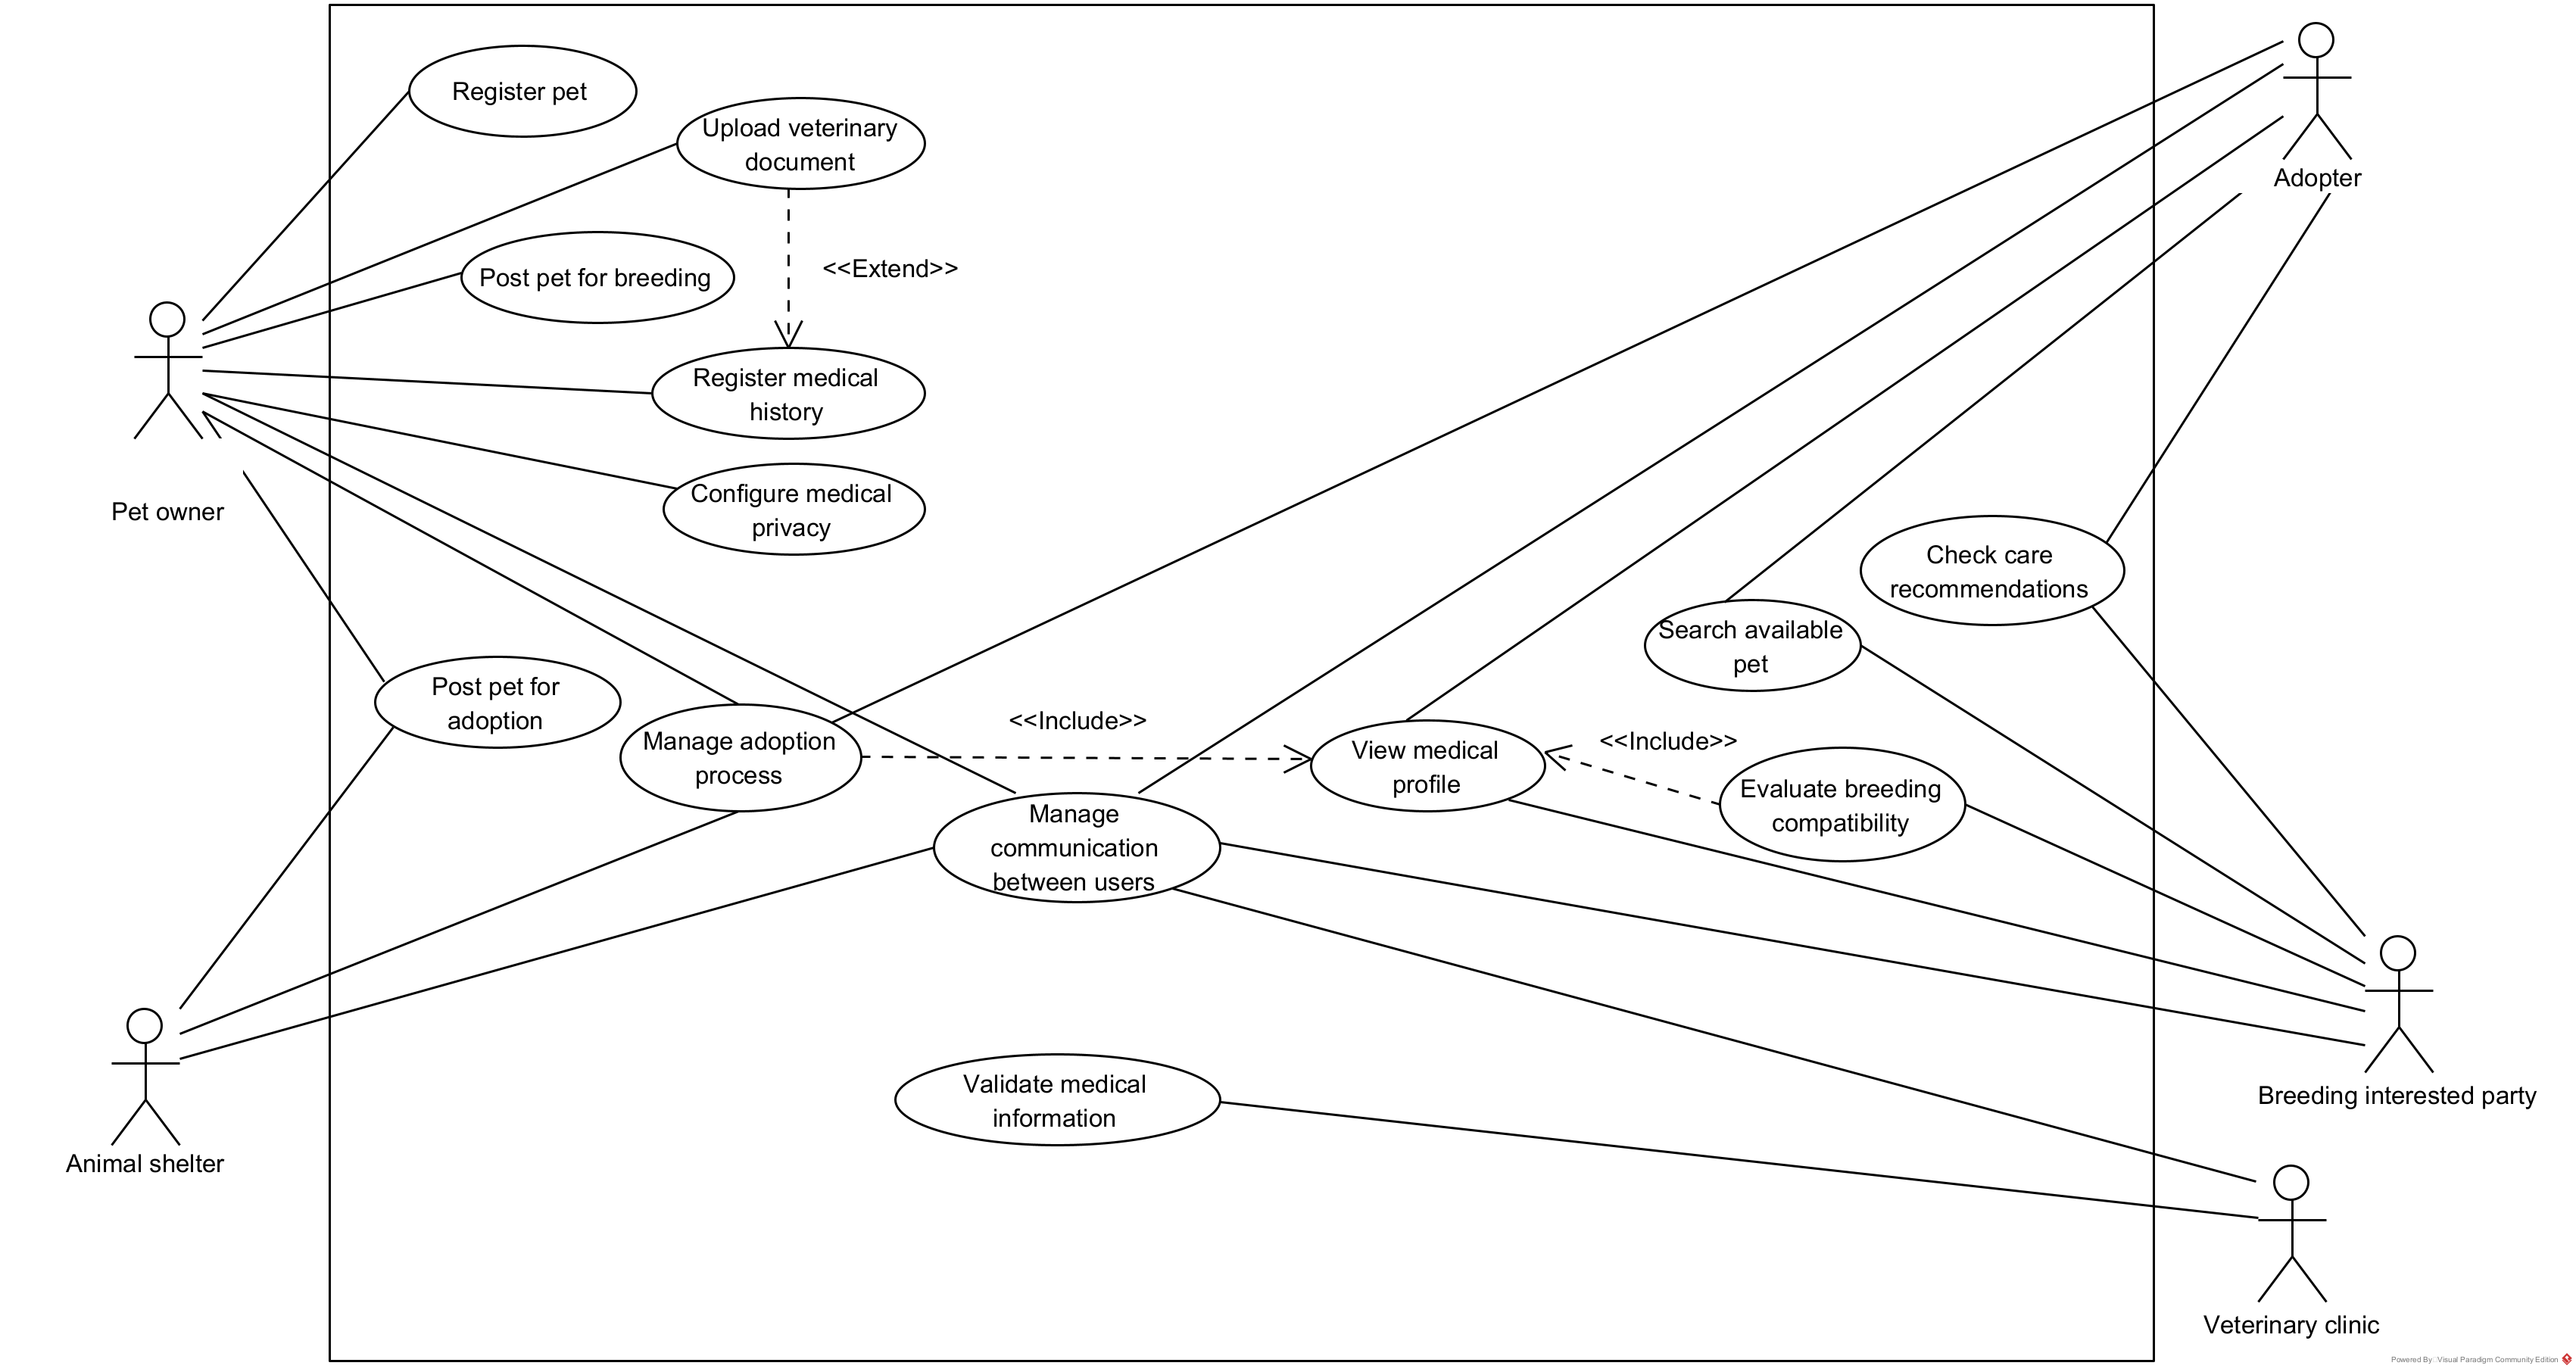
\includegraphics[width=1\textwidth]{figuras/DiagramaCasosDeUso_MundiPets.png}
		\caption{Diagrama de casos de uso general del sistema MundiPets.}
		\label{fig:cu-general}
	\end{figure}
	
	% ------------------------------------------------------------
	\subsection{Especificación textual de casos de uso}
	\label{sec:cu-detallado}
	
	A continuación se especifican textualmente los trece casos de uso derivados
	de los requisitos funcionales de prioridad \emph{Debe tener} (Must) y de
	aquellos requisitos \emph{Debería tener} (Should) que resultan
	indispensables para completar los flujos de adopción y cruza. Cada
	especificación sigue la plantilla de la asignatura y mantiene la
	trazabilidad explícita hacia los requisitos de la
	Sección~\ref{sec:rf}. Los diagramas de secuencia
	(Sección~\ref{sec:secuencia}) y de actividad
	(Sección~\ref{sec:actividad}) se corresponden uno a uno con estos casos de
	uso.
	
	\begin{atributos}{CU-01}{CU-01 --- Registrar mascota.}
		Identificador & CU-01 \\
		Nombre & Registrar mascota \\
		Actor principal & Propietario de mascota \\
		Actores secundarios & Refugio de animales; componente de validación de imágenes \\
		RF asociados & RF-01, RF-17, RF-21 \\
		Precondiciones & El propietario está autenticado y su identidad ha sido verificada (RF-12). \\
		Flujo principal &
		\begin{enumerate}[leftmargin=*, nosep]
			\item El propietario accede al formulario de registro de mascota.
			\item El sistema presenta los campos obligatorios y opcionales.
			\item El propietario ingresa nombre, especie, raza, sexo, edad y estado reproductivo.
			\item El propietario adjunta al menos una fotografía de la mascota.
			\item El sistema valida la completitud de los campos obligatorios.
			\item El sistema envía la fotografía al componente de validación de imágenes (RF-17).
			\item El componente confirma que la imagen corresponde a una mascota y es apropiada.
			\item El sistema almacena el perfil y confirma el registro al propietario.
		\end{enumerate} \\
		Flujos alternativos &
		\begin{enumerate}[leftmargin=*, nosep]
			\item[3.1] El propietario registra el identificador de microchip (RF-21); el sistema lo asocia al perfil.
			\item[8.1] El propietario decide no publicar la mascota; el perfil queda en estado \emph{Registrada}.
		\end{enumerate} \\
		Flujos de excepción &
		\begin{enumerate}[leftmargin=*, nosep]
			\item[5.1] Falta un campo obligatorio: el sistema retorna al formulario señalando el campo incompleto y no invoca la capa de persistencia.
			\item[7.1] La imagen es rechazada por el componente de IA: el sistema notifica el motivo del rechazo (RNF-14) y solicita una nueva fotografía.
		\end{enumerate} \\
		Postcondiciones & El perfil de la mascota queda almacenado en estado \emph{Registrada} y disponible para consulta, publicación y registro de historial médico. \\
	\end{atributos}
	
	\begin{atributos}{CU-02}{CU-02 --- Registrar historial médico y antecedentes genéticos.}
		Identificador & CU-02 \\
		Nombre & Registrar historial médico y antecedentes genéticos \\
		Actor principal & Propietario de mascota \\
		Actores secundarios & Veterinaria \\
		RF asociados & RF-02, RF-16, RF-24 \\
		Precondiciones & La mascota está registrada en el sistema (CU-01) y el usuario tiene permisos de escritura sobre su historial. \\
		Flujo principal &
		\begin{enumerate}[leftmargin=*, nosep]
			\item El usuario selecciona la mascota y accede a su historial médico.
			\item El sistema muestra el historial vigente y el formulario de registro.
			\item El usuario registra vacunas, desparasitaciones, enfermedades, alergias o tratamientos.
			\item El usuario ingresa la trazabilidad de cepa, lote y profesional aplicador de cada vacuna (RF-24).
			\item El usuario registra los antecedentes genéticos y de parentesco de la mascota (RF-16).
			\item El sistema valida el formato y la coherencia temporal de las fechas ingresadas.
			\item El sistema almacena el registro y actualiza el historial médico.
		\end{enumerate} \\
		Flujos alternativos &
		\begin{enumerate}[leftmargin=*, nosep]
			\item[7.1] Si quien registra es una \textbf{veterinaria} autorizada, el sistema marca el registro como validado profesionalmente (RD-03) e identifica al profesional responsable.
			\item[7.2] Si quien registra es el \textbf{propietario}, el registro queda en estado \emph{PendienteDeValidación} hasta que una veterinaria ejecute CU-09.
		\end{enumerate} \\
		Flujos de excepción &
		\begin{enumerate}[leftmargin=*, nosep]
			\item[6.1] La fecha de aplicación es posterior a la fecha actual: el sistema rechaza el registro y solicita corrección.
			\item[6.2] Falta la cepa o el aplicador de una vacuna: el sistema advierte que el registro no podrá ser validado profesionalmente mientras el dato esté ausente.
		\end{enumerate} \\
		Postcondiciones & El historial médico y los antecedentes genéticos quedan actualizados y disponibles para los usuarios autorizados según la configuración de privacidad (RF-11). \\
	\end{atributos}
	
	\begin{atributos}{CU-03}{CU-03 --- Cargar documento veterinario y carnet de vacunación.}
		Identificador & CU-03 \\
		Nombre & Cargar documento veterinario y carnet de vacunación \\
		Actor principal & Propietario de mascota \\
		Actores secundarios & Veterinaria (validación posterior) \\
		RF asociados & RF-14, RF-24 \\
		Precondiciones & La mascota está registrada y el propietario dispone del documento veterinario digitalizado. \\
		Flujo principal &
		\begin{enumerate}[leftmargin=*, nosep]
			\item El propietario accede a la sección de documentos de la mascota.
			\item El propietario adjunta el archivo del certificado o carnet de vacunación.
			\item El sistema valida el formato y el tamaño del archivo.
			\item El sistema extrae los metadatos del documento (tipo y fecha) y almacena el archivo.
			\item El sistema registra el documento en estado \emph{PendienteDeValidación}.
			\item El sistema actualiza el carnet de vacunación de la mascota y confirma la carga.
		\end{enumerate} \\
		Flujos alternativos &
		\begin{enumerate}[leftmargin=*, nosep]
			\item[4.1] Los metadatos no pueden extraerse automáticamente: el sistema solicita al propietario que ingrese manualmente el tipo y la fecha del documento.
			\item[6.1] Ya existe un documento vigente del mismo tipo: el sistema conserva el anterior como versión histórica y marca el nuevo como vigente.
		\end{enumerate} \\
		Flujos de excepción &
		\begin{enumerate}[leftmargin=*, nosep]
			\item[3.1] El formato del archivo no es admitido o excede el tamaño máximo: el sistema rechaza la carga e informa la restricción.
		\end{enumerate} \\
		Postcondiciones & El documento queda almacenado y visible para el propietario, en estado \emph{PendienteDeValidación} hasta la ejecución de CU-09 por parte de una veterinaria autorizada. \\
	\end{atributos}
	
	\begin{atributos}{CU-04}{CU-04 --- Publicar mascota en adopción.}
		Identificador & CU-04 \\
		Nombre & Publicar mascota en adopción \\
		Actor principal & Propietario de mascota \\
		Actores secundarios & Refugio de animales \\
		RF asociados & RF-13, RF-05 \\
		Precondiciones & La mascota está registrada (CU-01) y el propietario es su titular en el sistema. \\
		Flujo principal &
		\begin{enumerate}[leftmargin=*, nosep]
			\item El propietario selecciona una mascota registrada.
			\item El propietario indica el tipo de disponibilidad: adopción.
			\item El sistema verifica la completitud del perfil (fotografías, vacunas, datos generales).
			\item El sistema habilita la confirmación de la publicación.
			\item El propietario confirma la publicación.
			\item El sistema crea la publicación y la incorpora al listado de mascotas disponibles.
		\end{enumerate} \\
		Flujos alternativos &
		\begin{enumerate}[leftmargin=*, nosep]
			\item[1.1] La mascota ya cuenta con una publicación activa: el sistema ofrece actualizar la publicación existente en lugar de crear un duplicado.
			\item[3.1] El perfil está incompleto: el sistema muestra una advertencia preventiva con los campos faltantes, sin bloquear la publicación.
		\end{enumerate} \\
		Flujos de excepción &
		\begin{enumerate}[leftmargin=*, nosep]
			\item[6.1] La mascota se encuentra en estado \emph{EnProcesoDeAdopción} o \emph{Adoptada}: el sistema impide la publicación e informa el estado vigente.
		\end{enumerate} \\
		Postcondiciones & La mascota transita al estado \emph{Publicada} y queda visible en las búsquedas de adopción (CU-11). \\
	\end{atributos}
	
	\begin{atributos}{CU-05}{CU-05 --- Publicar mascota para cruza y gestionar solicitud.}
		Identificador & CU-05 \\
		Nombre & Publicar mascota para cruza y gestionar solicitud \\
		Actor principal & Propietario de mascota \\
		Actores secundarios & Interesado en cruza \\
		RF asociados & RF-08, RF-13, RF-16, RF-19 \\
		Precondiciones & La mascota está registrada y cuenta con antecedentes genéticos registrados (RF-16). \\
		Flujo principal &
		\begin{enumerate}[leftmargin=*, nosep]
			\item El propietario selecciona la mascota e indica disponibilidad para cruza.
			\item El sistema verifica que existan antecedentes genéticos y de parentesco registrados.
			\item El sistema verifica la vigencia del certificado veterinario asociado (RF-19).
			\item El sistema publica la mascota en el listado de cruza responsable.
			\item Un interesado en cruza envía una solicitud sobre la publicación.
			\item El sistema registra la solicitud en estado \emph{Pendiente} y notifica al propietario.
			\item El propietario acepta o rechaza la solicitud.
			\item El sistema actualiza el estado de la solicitud y notifica al interesado.
		\end{enumerate} \\
		Flujos alternativos &
		\begin{enumerate}[leftmargin=*, nosep]
			\item[2.1] No existen antecedentes genéticos: el sistema redirige al propietario al formulario de RF-16 antes de permitir continuar.
			\item[7.1] El propietario acepta: el sistema habilita el canal de comunicación (CU-08) y la mascota transita a \emph{EnProcesoDeCruza}.
		\end{enumerate} \\
		Flujos de excepción &
		\begin{enumerate}[leftmargin=*, nosep]
			\item[3.1] El certificado veterinario está vencido o no validado: el sistema impide la publicación e informa el requisito pendiente.
		\end{enumerate} \\
		Postcondiciones & La publicación de cruza queda activa y las solicitudes recibidas quedan registradas con su estado y fecha para su consulta posterior (CU-07). \\
	\end{atributos}
	
	\begin{atributos}{CU-06}{CU-06 --- Evaluar compatibilidad de cruza.}
		Identificador & CU-06 \\
		Nombre & Evaluar compatibilidad de cruza \\
		Actor principal & Interesado en cruza \\
		Actores secundarios & Propietario de mascota; componente de inteligencia artificial \\
		RF asociados & RF-06, RF-16, RF-23 \\
		Precondiciones & Ambas mascotas están registradas, publicadas para cruza y cuentan con historial médico y antecedentes genéticos. \\
		Flujo principal &
		\begin{enumerate}[leftmargin=*, nosep]
			\item El usuario selecciona las dos mascotas a comparar.
			\item El sistema recupera los datos generales, el historial médico y los antecedentes genéticos de ambas.
			\item El sistema ejecuta la verificación de parentesco (CU-13).
			\item El sistema envía los datos al componente de evaluación de compatibilidad.
			\item El componente calcula el resultado orientativo y genera la explicación causal asociada (RNF-13).
			\item El sistema presenta el resultado junto con los factores que lo sustentan.
			\item El sistema registra la evaluación para su consulta posterior.
		\end{enumerate} \\
		Flujos alternativos &
		\begin{enumerate}[leftmargin=*, nosep]
			\item[3.1] Se detecta un grado de parentesco incompatible: el sistema muestra una alerta explícita (RF-23) y finaliza sin generar recomendación.
			\item[6.1] El resultado indica riesgo sanitario: el sistema adjunta la alerta correspondiente antes de mostrar el resultado.
		\end{enumerate} \\
		Flujos de excepción &
		\begin{enumerate}[leftmargin=*, nosep]
			\item[2.1] Una de las mascotas carece de antecedentes genéticos: el sistema informa que la evaluación no puede realizarse y señala la información faltante.
			\item[5.1] El componente de IA no responde dentro del umbral definido en RNF-03: el sistema informa la indisponibilidad temporal del servicio.
		\end{enumerate} \\
		Postcondiciones & El usuario dispone de un resultado orientativo de compatibilidad con su explicación causal; el resultado no sustituye la valoración profesional veterinaria. \\
	\end{atributos}
	
	\begin{atributos}{CU-07}{CU-07 --- Consultar historial de procesos de adopción y cruza.}
		Identificador & CU-07 \\
		Nombre & Consultar historial de procesos de adopción y cruza \\
		Actor principal & Propietario de mascota \\
		Actores secundarios & Refugio de animales \\
		RF asociados & RF-15, RF-05, RF-08 \\
		Precondiciones & El propietario está autenticado y posee al menos una mascota con solicitudes registradas. \\
		Flujo principal &
		\begin{enumerate}[leftmargin=*, nosep]
			\item El propietario accede a la sección de historial de procesos.
			\item El sistema recupera en paralelo las solicitudes de adopción y de cruza asociadas a sus mascotas.
			\item El sistema combina ambos conjuntos en una línea de tiempo ordenada por fecha.
			\item El sistema determina, para cada solicitud, el nivel de información visible según su estado.
			\item El sistema presenta el historial consolidado con el estado vigente de cada proceso.
		\end{enumerate} \\
		Flujos alternativos &
		\begin{enumerate}[leftmargin=*, nosep]
			\item[5.1] El propietario filtra el historial por mascota, tipo de proceso o rango de fechas.
		\end{enumerate} \\
		Flujos de excepción &
		\begin{enumerate}[leftmargin=*, nosep]
			\item[2.1] No existen solicitudes registradas: el sistema muestra un mensaje informativo en lugar de una lista vacía.
		\end{enumerate} \\
		Postcondiciones & El propietario visualiza la trazabilidad completa de sus procesos sin que se expongan datos de contacto de solicitantes no aceptados, en cumplimiento del principio de minimización de datos (RL-05). \\
	\end{atributos}
	
	\begin{atributos}{CU-08}{CU-08 --- Gestionar comunicación entre usuarios.}
		Identificador & CU-08 \\
		Nombre & Gestionar comunicación entre usuarios \\
		Actor principal & Propietario de mascota, Adoptante, Interesado en cruza \\
		Actores secundarios & Refugio de animales; componente de moderación automática \\
		RF asociados & RF-07 \\
		Precondiciones & Existe una solicitud de adopción o cruza que habilita el canal de comunicación entre ambas partes. \\
		Flujo principal &
		\begin{enumerate}[leftmargin=*, nosep]
			\item El usuario abre la conversación asociada a la solicitud.
			\item El usuario redacta y envía un mensaje.
			\item El sistema envía el contenido al componente de moderación automática.
			\item El componente clasifica el mensaje como apropiado.
			\item El sistema almacena el mensaje y lo entrega al destinatario.
			\item El sistema notifica al destinatario la recepción del mensaje.
		\end{enumerate} \\
		Flujos alternativos &
		\begin{enumerate}[leftmargin=*, nosep]
			\item[2.1] El usuario adjunta una imagen; el sistema la somete a la validación de imágenes (RF-17) antes de la moderación de texto.
		\end{enumerate} \\
		Flujos de excepción &
		\begin{enumerate}[leftmargin=*, nosep]
			\item[4.1] El mensaje es marcado como inapropiado: el sistema bloquea el envío y notifica al remitente la categoría de infracción detectada conforme a RNF-15, sin entregarlo al destinatario.
			\item[5.1] El destinatario ha bloqueado la conversación: el sistema impide el envío e informa al remitente.
		\end{enumerate} \\
		Postcondiciones & Únicamente los mensajes que superan la moderación quedan persistidos y disponibles en el historial de la conversación. \\
	\end{atributos}
	
	\begin{atributos}{CU-09}{CU-09 --- Validar información médica.}
		Identificador & CU-09 \\
		Nombre & Validar información médica \\
		Actor principal & Veterinaria \\
		Actores secundarios & Propietario de mascota \\
		RF asociados & RF-09, RF-14, RF-24 \\
		Precondiciones & La veterinaria está autenticada, su identidad profesional ha sido verificada (RF-12) y existe información médica en estado \emph{PendienteDeValidación}. \\
		Flujo principal &
		\begin{enumerate}[leftmargin=*, nosep]
			\item La veterinaria accede a la bandeja de registros pendientes de validación.
			\item La veterinaria selecciona el historial médico o documento a revisar.
			\item El sistema muestra el registro junto con el documento adjunto.
			\item La veterinaria contrasta la información y aprueba el registro.
			\item El sistema marca el registro como \emph{Validado} y asocia la identificación del profesional responsable.
			\item El sistema notifica al propietario el resultado de la validación.
		\end{enumerate} \\
		Flujos alternativos &
		\begin{enumerate}[leftmargin=*, nosep]
			\item[4.1] La veterinaria rechaza el registro: el sistema exige el ingreso de una observación técnica antes de confirmar la operación y el registro transita a \emph{Rechazado}.
		\end{enumerate} \\
		Flujos de excepción &
		\begin{enumerate}[leftmargin=*, nosep]
			\item[4.2] La veterinaria intenta rechazar sin observación técnica: el sistema impide confirmar la operación e indica el campo obligatorio.
			\item[3.1] El documento adjunto es ilegible: la veterinaria registra la observación correspondiente y el registro se devuelve al propietario para su reemplazo.
		\end{enumerate} \\
		Postcondiciones & El registro médico queda en estado \emph{Validado} o \emph{Rechazado} con trazabilidad del profesional responsable y de la fecha de la resolución, en cumplimiento de RD-03 y RNF-05. \\
	\end{atributos}
	
	\begin{atributos}{CU-10}{CU-10 --- Consultar perfil médico.}
		Identificador & CU-10 \\
		Nombre & Consultar perfil médico \\
		Actor principal & Adoptante, Interesado en cruza \\
		Actores secundarios & Propietario de mascota, Veterinaria \\
		RF asociados & RF-03, RF-11 \\
		Precondiciones & La mascota existe en el sistema y el usuario consultante está autenticado. \\
		Flujo principal &
		\begin{enumerate}[leftmargin=*, nosep]
			\item El usuario selecciona una mascota desde el resultado de una búsqueda o publicación.
			\item El sistema determina el nivel de acceso del usuario consultante.
			\item El sistema recupera los datos generales, el historial médico y las fotografías de la mascota.
			\item El sistema aplica las reglas de privacidad configuradas por el propietario (RF-11).
			\item El sistema filtra la ubicación exacta y los datos de contacto directo, mostrando únicamente la zona aproximada (RNF-16).
			\item El sistema presenta el perfil resultante al usuario.
		\end{enumerate} \\
		Flujos alternativos &
		\begin{enumerate}[leftmargin=*, nosep]
			\item[2.1] El consultante es el propietario: el sistema muestra el perfil completo sin filtrado.
			\item[2.2] El consultante es una veterinaria autorizada: el sistema muestra los campos médicos obligatorios aun cuando el propietario los haya restringido para otros roles (RD-03).
		\end{enumerate} \\
		Flujos de excepción &
		\begin{enumerate}[leftmargin=*, nosep]
			\item[3.1] La publicación fue retirada o la mascota fue eliminada: el sistema informa que el perfil ya no está disponible.
		\end{enumerate} \\
		Postcondiciones & El usuario obtiene la información autorizada necesaria para tomar una decisión informada sobre adopción o cruza, sin exposición de datos sensibles restringidos. \\
	\end{atributos}
	
	\begin{atributos}{CU-11}{CU-11 --- Buscar mascota disponible.}
		Identificador & CU-11 \\
		Nombre & Buscar mascota disponible \\
		Actor principal & Adoptante, Interesado en cruza \\
		Actores secundarios & --- \\
		RF asociados & RF-04, RF-13 \\
		Precondiciones & Existen publicaciones activas de mascotas en el sistema. \\
		Flujo principal &
		\begin{enumerate}[leftmargin=*, nosep]
			\item El usuario accede al buscador de mascotas.
			\item El usuario selecciona los criterios de filtrado: especie, raza, edad, ubicación aproximada, tamaño, temperamento y tipo de disponibilidad.
			\item El sistema consulta el repositorio de publicaciones activas.
			\item El sistema aplica de forma acumulativa todos los filtros seleccionados.
			\item El sistema ordena los resultados por relevancia o cercanía.
			\item El sistema presenta la lista de mascotas coincidentes.
		\end{enumerate} \\
		Flujos alternativos &
		\begin{enumerate}[leftmargin=*, nosep]
			\item[6.1] El usuario selecciona una mascota del listado e invoca CU-10 para consultar su perfil.
		\end{enumerate} \\
		Flujos de excepción &
		\begin{enumerate}[leftmargin=*, nosep]
			\item[5.1] No existen coincidencias: el sistema informa el resultado vacío y ofrece ajustar o relajar los criterios antes de repetir la búsqueda.
		\end{enumerate} \\
		Postcondiciones & El usuario obtiene un conjunto de publicaciones que cumplen simultáneamente todos los criterios aplicados. \\
	\end{atributos}
	
	\begin{atributos}{CU-12}{CU-12 --- Configurar privacidad médica.}
		Identificador & CU-12 \\
		Nombre & Configurar privacidad médica \\
		Actor principal & Propietario de mascota \\
		Actores secundarios & Veterinaria (destinataria de la excepción de visibilidad) \\
		RF asociados & RF-11, RF-03 \\
		Precondiciones & El propietario está autenticado y posee al menos una mascota registrada. \\
		Flujo principal &
		\begin{enumerate}[leftmargin=*, nosep]
			\item El propietario accede a la configuración de privacidad de la mascota.
			\item El sistema muestra las categorías de datos sensibles: ubicación, contacto y afecciones específicas.
			\item El propietario define el nivel de visibilidad para cada categoría y rol.
			\item El sistema verifica si alguno de los campos restringidos es obligatorio para la validación veterinaria.
			\item El sistema guarda la configuración y confirma la operación.
			\item El sistema aplica las nuevas reglas a todas las consultas posteriores (CU-10).
		\end{enumerate} \\
		Flujos alternativos &
		\begin{enumerate}[leftmargin=*, nosep]
			\item[4.1] Un campo médico obligatorio ha sido restringido: el sistema muestra una advertencia, conserva ese campo visible para las veterinarias autorizadas y guarda el resto de la configuración con normalidad.
		\end{enumerate} \\
		Flujos de excepción &
		\begin{enumerate}[leftmargin=*, nosep]
			\item[5.1] La configuración no puede almacenarse: el sistema conserva la configuración anterior e informa el error, evitando estados de privacidad indeterminados.
		\end{enumerate} \\
		Postcondiciones & La configuración de privacidad queda vigente y se aplica de forma inmediata sobre todas las consultas del perfil, garantizando la visibilidad mínima exigida por RD-03. \\
	\end{atributos}
	
	\begin{atributos}{CU-13}{CU-13 --- Verificación de parentesco previa a la evaluación de compatibilidad.}
		Identificador & CU-13 \\
		Nombre & Evaluar compatibilidad de cruza --- verificación de parentesco \\
		Actor principal & Interesado en cruza \\
		Actores secundarios & Propietario de mascota; componente de inteligencia artificial \\
		RF asociados & RF-06, RF-16, RF-23 \\
		Precondiciones & Ambas mascotas cuentan con antecedentes genéticos y de linaje registrados (RF-16). \\
		Flujo principal &
		\begin{enumerate}[leftmargin=*, nosep]
			\item El sistema recibe la solicitud de evaluación con las dos mascotas seleccionadas.
			\item El sistema recupera el linaje declarado de ambas mascotas.
			\item El sistema ejecuta una comprobación determinística del grado de parentesco.
			\item El sistema determina que no existe incompatibilidad por parentesco.
			\item El sistema habilita la invocación del componente de evaluación de compatibilidad (CU-06).
		\end{enumerate} \\
		Flujos alternativos &
		\begin{enumerate}[leftmargin=*, nosep]
			\item[3.1] Se detecta un grado de parentesco incompatible: el flujo se dirige a la actividad de alerta explícita, se notifica al usuario y se finaliza sin invocar el componente de IA ni generar recomendación alguna.
		\end{enumerate} \\
		Flujos de excepción &
		\begin{enumerate}[leftmargin=*, nosep]
			\item[2.1] El linaje de alguna de las mascotas es desconocido o está incompleto: el sistema advierte que la verificación no es concluyente y deja constancia de la limitación junto al resultado.
		\end{enumerate} \\
		Postcondiciones & La evaluación de compatibilidad solo se ejecuta sobre parejas sin incompatibilidad de parentesco, optimizando el uso del componente de IA y evitando recomendaciones inviables por regla de negocio. \\
	\end{atributos}
	
	% ------------------------------------------------------------
	\subsection{Diagrama de clases refinado}
	\label{sec:clases-refinado}
	
	El diagrama de clases refinado profundiza el modelo conceptual presentado en
	la Entrega 2 (1B), incorporando los atributos, tipos de dato,
	multiplicidades y operaciones necesarios para representar con precisión las
	25 funcionalidades definidas en la Sección~\ref{sec:rf}. El modelo se
	organiza alrededor de la clase \texttt{Mascota}, que concentra los datos
	generales exigidos por RF-01 (nombre, especie, raza, sexo, edad y estado
	reproductivo) y se asocia mediante composición con \texttt{HistorialMedico}
	(RF-02, RF-14, RF-24), \texttt{AntecedenteGenetico} (RF-16) y
	\texttt{Microchip} (RF-21), reflejando que estos objetos no tienen sentido
	de existencia fuera de la mascota a la que pertenecen.
	
	Las clases \texttt{Usuario}, \texttt{PropietarioMascota},
	\texttt{Adoptante}, \texttt{InteresadoEnCruza}, \texttt{RefugioAnimal} y
	\texttt{Veterinaria} se modelan mediante una jerarquía de generalización a
	partir de \texttt{Usuario}, que centraliza los atributos comunes de
	autenticación y verificación de identidad (RF-12) y evita duplicar reglas de
	acceso entre los distintos roles descritos en RD-02. La clase
	\texttt{SolicitudAdopcion} incorpora los atributos de etapa exigidos por
	RF-18 (formulario, entrevista, visita, periodo de prueba y compromiso
	firmado), mientras que \texttt{SolicitudCruza} se asocia con
	\texttt{RegistroCompatibilidad} para representar el resultado orientativo
	generado por el componente de inteligencia artificial (RF-06) y con
	\texttt{CertificadoVeterinario} para reflejar la validación previa exigida
	por RF-19.
	
	Las clases \texttt{Publicacion}, \texttt{Mensaje}, \texttt{AlertaRiesgo} y
	\texttt{AvisoExtraviado} completan el modelo, cubriendo respectivamente
	RF-13, RF-07, RF-23 y RF-25. Las multiplicidades reflejan las reglas de
	negocio ya validadas en el ERS: una mascota puede tener múltiples registros
	de historial médico pero pertenece a un único propietario; una solicitud de
	cruza involucra exactamente dos mascotas; y un aviso de extravío se asocia
	con una sola mascota registrada. Este nivel de detalle permite que el
	diagrama sirva como referencia directa para el diseño del modelo de datos en
	la fase de implementación.
	
	\begin{figure}[H]
		\centering
		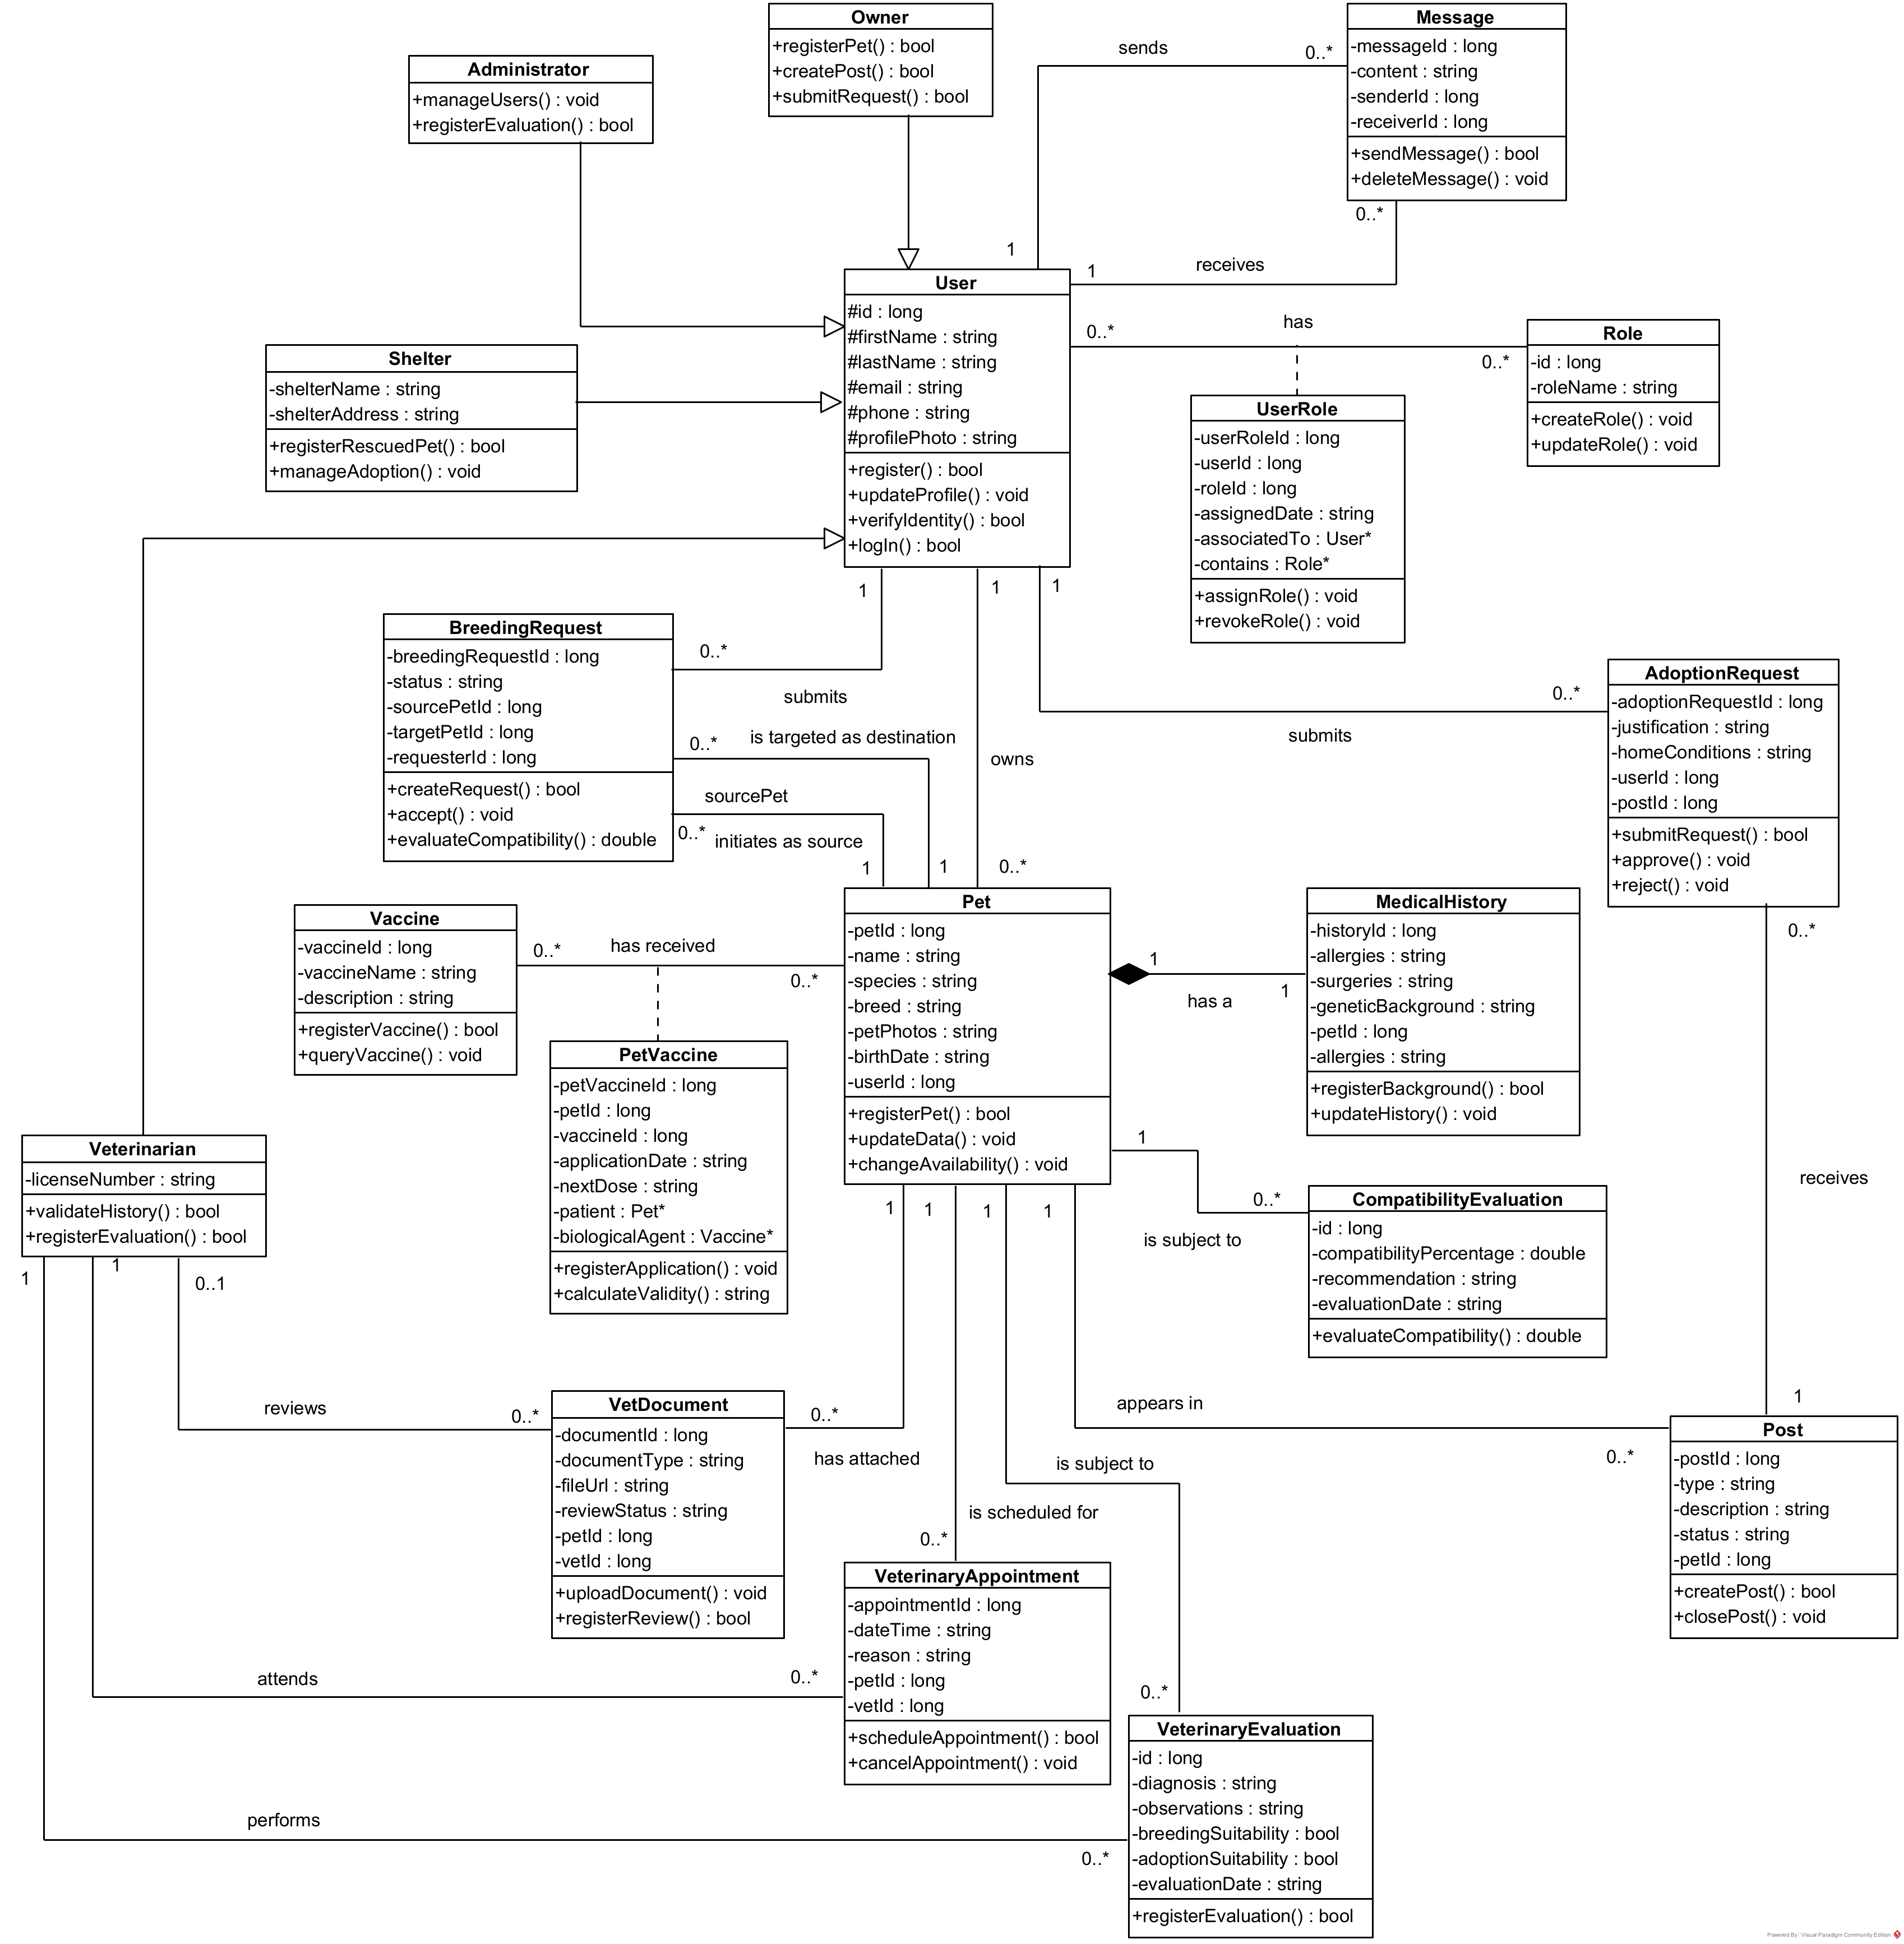
\includegraphics[width=0.72\textwidth]{figuras/DiagramaClasesRefinado_MundiPets.png}
		\caption{Diagrama de clases refinado del sistema MundiPets.}
		\label{fig:clases-refinado}
	\end{figure}
	
	% ------------------------------------------------------------
	\subsection{Diagramas de secuencia}
	\label{sec:secuencia}
	
	Los diagramas de secuencia detallan la interacción temporal entre los
	actores y los objetos del sistema para los trece casos de uso especificados
	textualmente en la Sección~\ref{sec:cu-detallado}, mostrando el orden de los
	mensajes intercambiados entre el actor, la interfaz, el controlador y los
	objetos de dominio involucrados en cada operación. A continuación se
	presentan los trece diagramas completos (CU-01 a CU-13).
	
	\subsubsection{Registrar mascota (CU-01)}
	
	El diagrama de secuencia de CU-01 ilustra el flujo mediante el cual el
	propietario, ya autenticado, ingresa los datos generales de la mascota y
	adjunta al menos una fotografía. La interfaz delega en el controlador la
	validación de los campos obligatorios definidos en RF-01; ante un campo
	faltante, el controlador retorna el mensaje de error correspondiente sin
	invocar la capa de persistencia, evitando así el registro de perfiles
	incompletos. Cuando la validación es exitosa, el controlador invoca al
	componente de validación de imágenes (RF-17) antes de confirmar el
	almacenamiento del perfil, de modo que ninguna fotografía llega a
	persistirse sin haber sido evaluada por el módulo de inteligencia
	artificial.
	
	\begin{figure}[H]
		\centering
		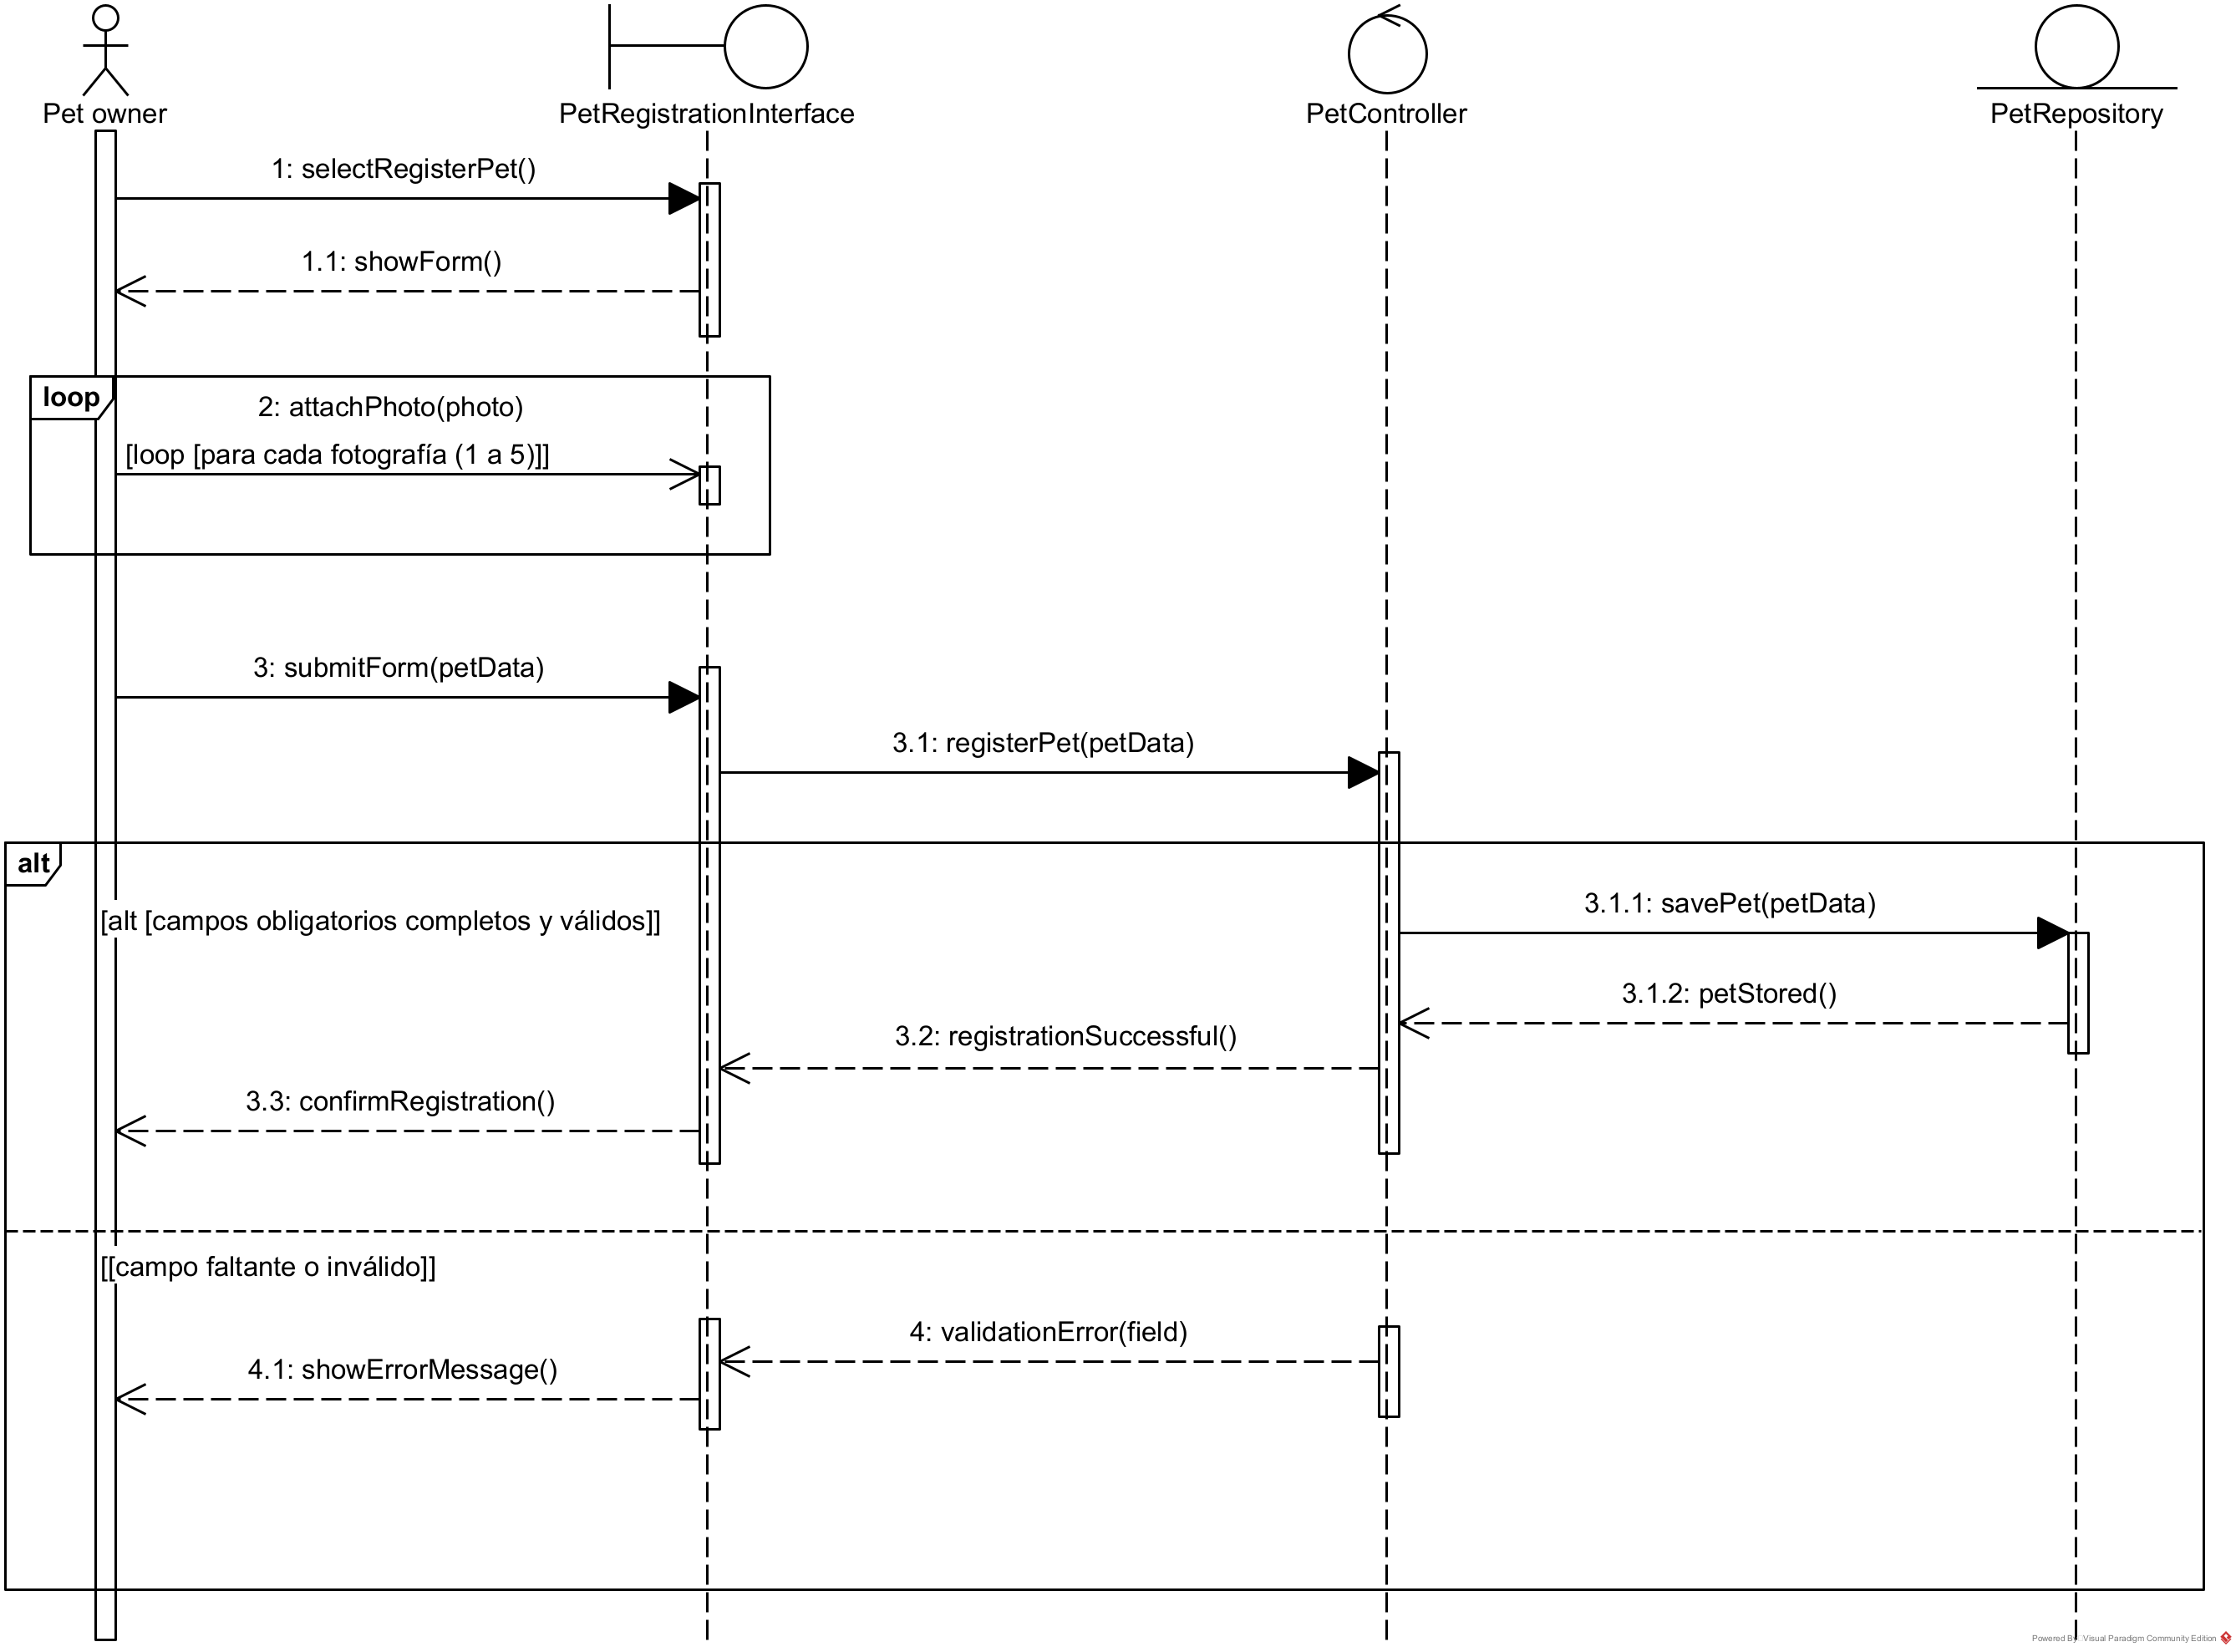
\includegraphics[width=0.72\textwidth]{figuras/DiagramaSecuencia_CU-01_MundiPets.png}
		\caption{Diagrama de secuencia del caso de uso CU-01 --- Registrar mascota.}
		\label{fig:sec-cu01}
	\end{figure}
	
	\subsubsection{Registrar historial médico y antecedentes genéticos (CU-02)}
	
	Este diagrama modela la interacción entre el propietario o la veterinaria y
	el sistema al registrar vacunas, desparasitaciones, enfermedades, alergias,
	tratamientos y antecedentes genéticos o de parentesco (RF-02, RF-16),
	incluyendo la trazabilidad de cepa, lote y aplicador exigida por RF-24. La
	secuencia muestra explícitamente la bifurcación de actor: cuando quien
	registra la información es una veterinaria, el mensaje de confirmación
	adicionalmente marca el campo de validación profesional (RD-03), mientras
	que si el emisor es el propietario, el registro queda almacenado con estado
	pendiente de validación hasta que una veterinaria lo revise.
	
	\begin{figure}[H]
		\centering
		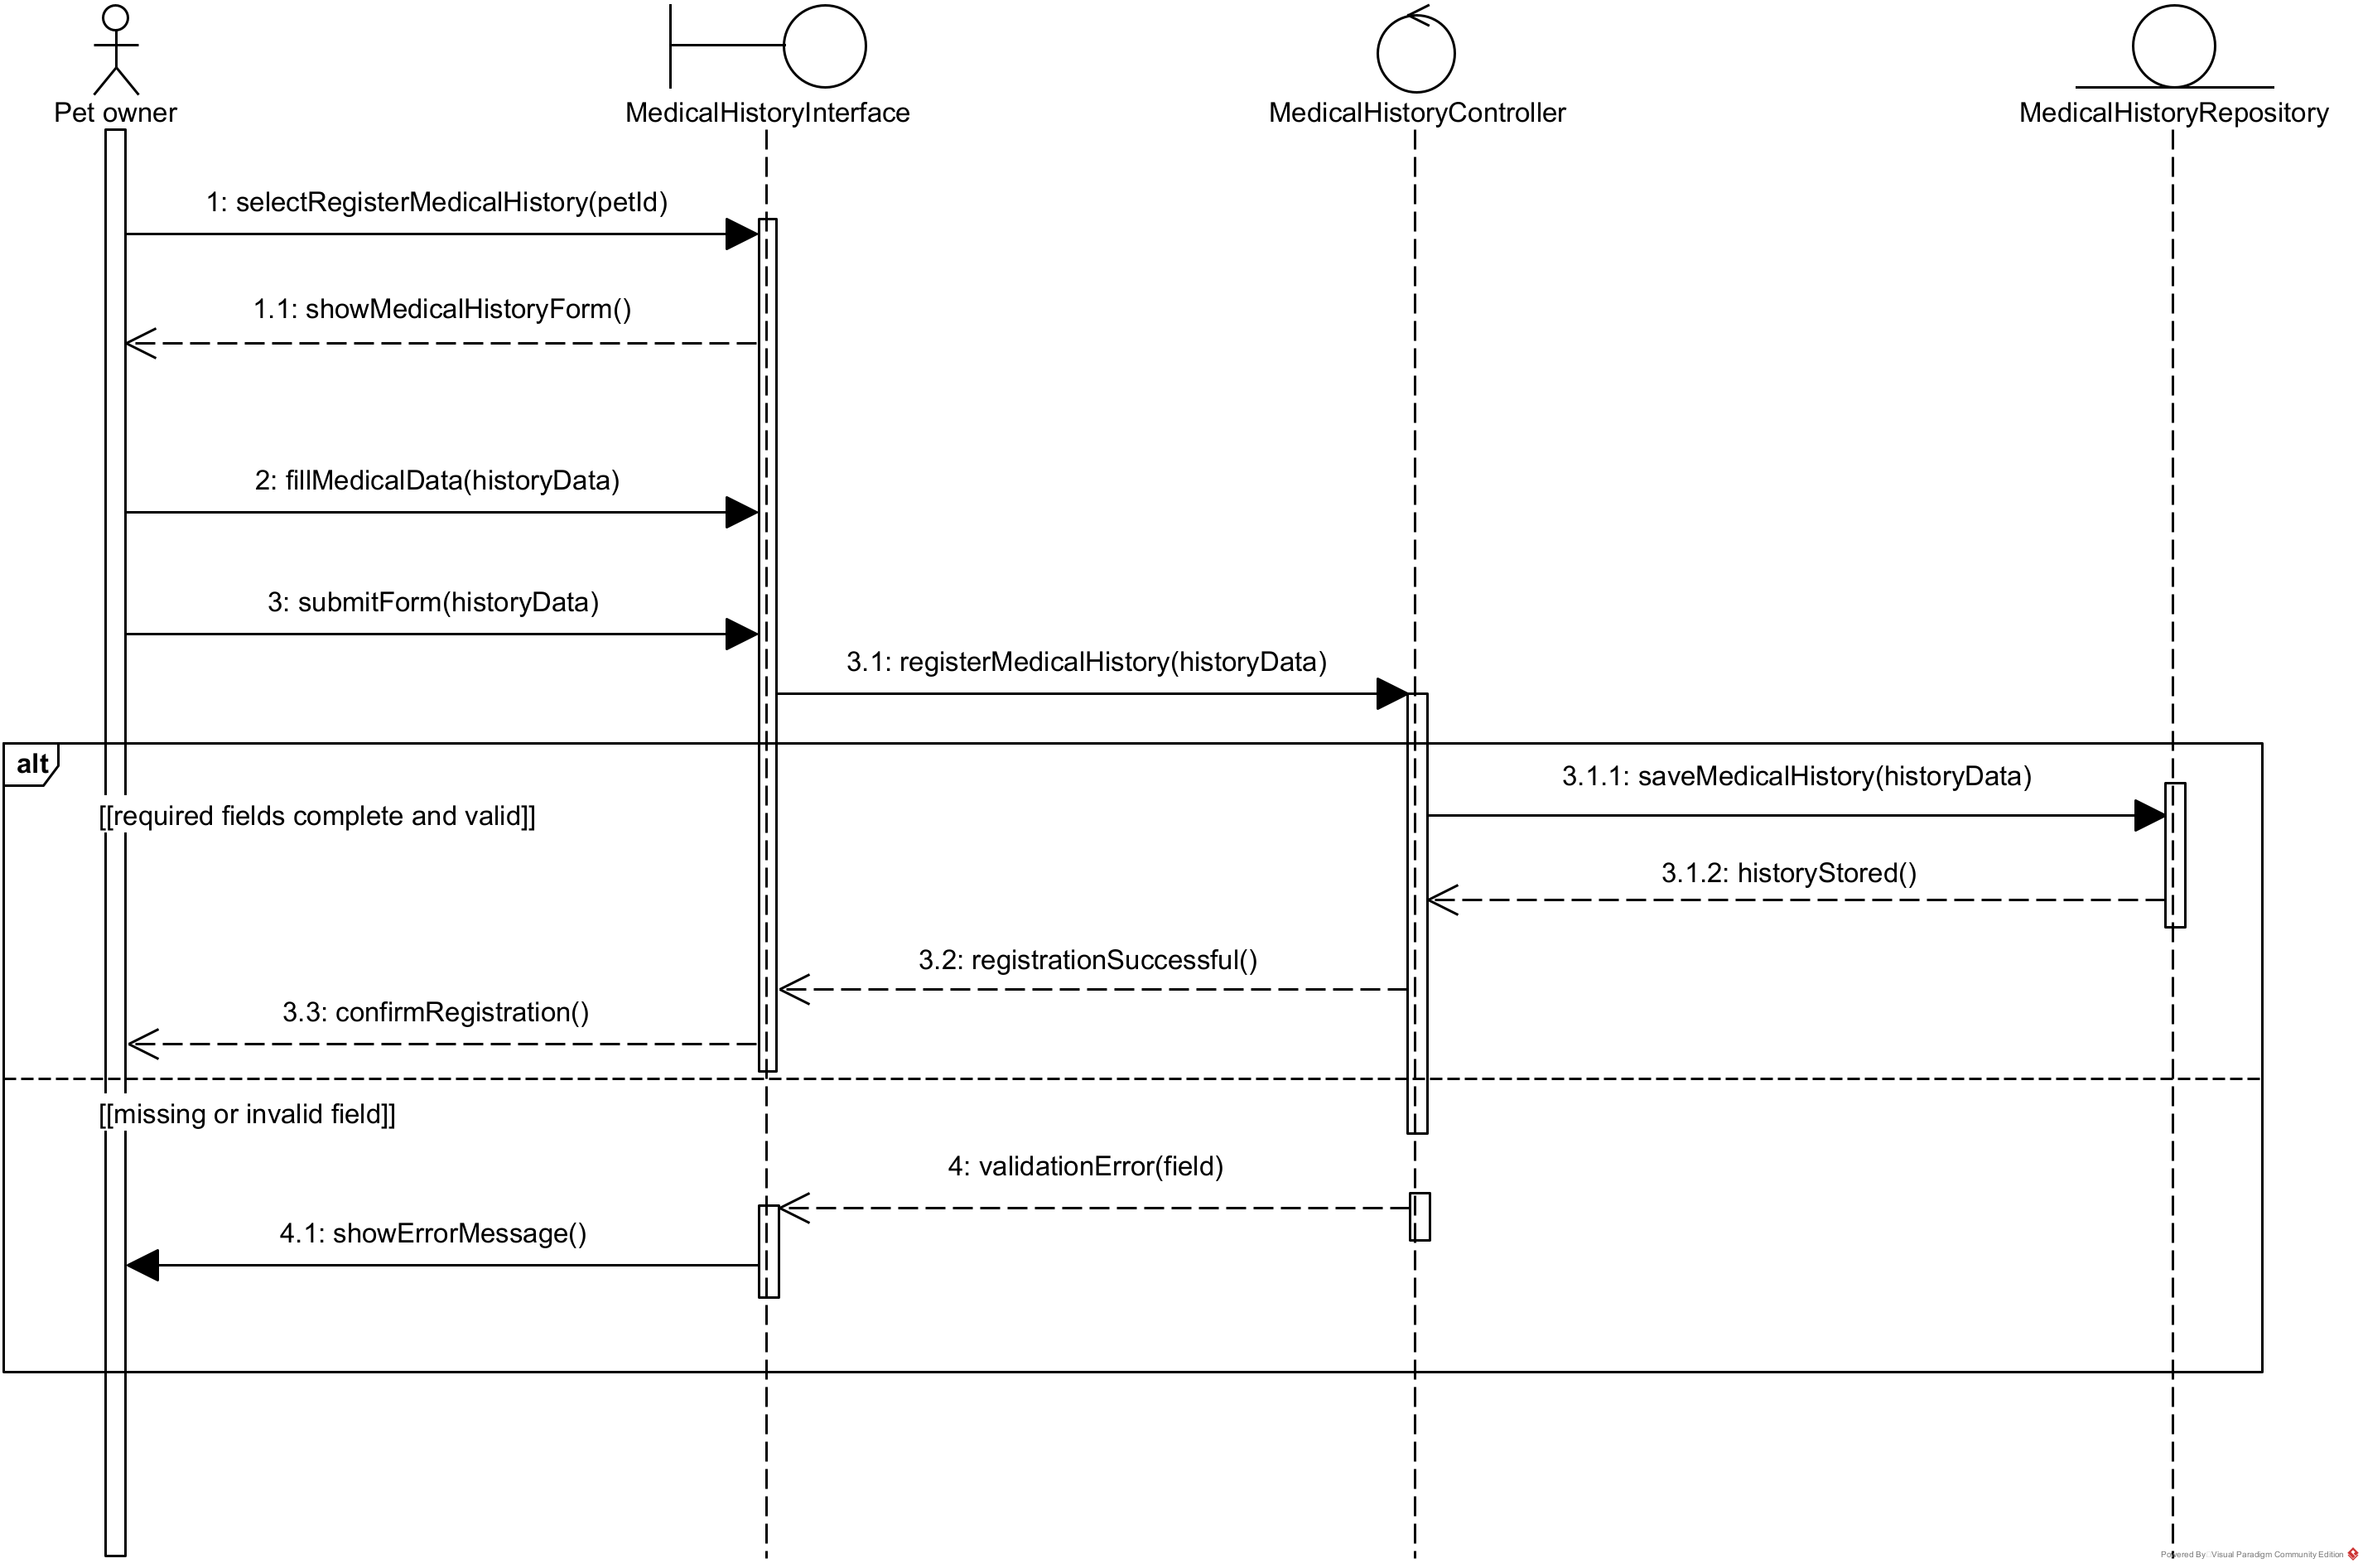
\includegraphics[width=0.72\textwidth]{figuras/DiagramaSecuencia_CU-02_MundiPets.png}
		\caption{Diagrama de secuencia del caso de uso CU-02 --- Registrar historial médico y antecedentes genéticos.}
		\label{fig:sec-cu02}
	\end{figure}
	
	\subsubsection{Cargar documento veterinario y carnet de vacunación (CU-03)}
	
	El diagrama de secuencia de CU-03 detalla la carga de documentos
	veterinarios digitalizados y la actualización del carnet de vacunación de la
	mascota (RF-14). El propietario adjunta el archivo desde la interfaz, la
	cual delega en el controlador el almacenamiento del documento con estado
	inicial pendiente de revisión. La secuencia refleja que el documento queda
	disponible de inmediato para consulta por el propietario, pero su estado de
	vigencia solo se actualiza a validado una vez que una veterinaria autorizada
	ejecuta el caso de uso CU-09 sobre dicho archivo, evitando que dos flujos
	distintos escriban simultáneamente sobre el mismo estado.
	
	\begin{figure}[H]
		\centering
		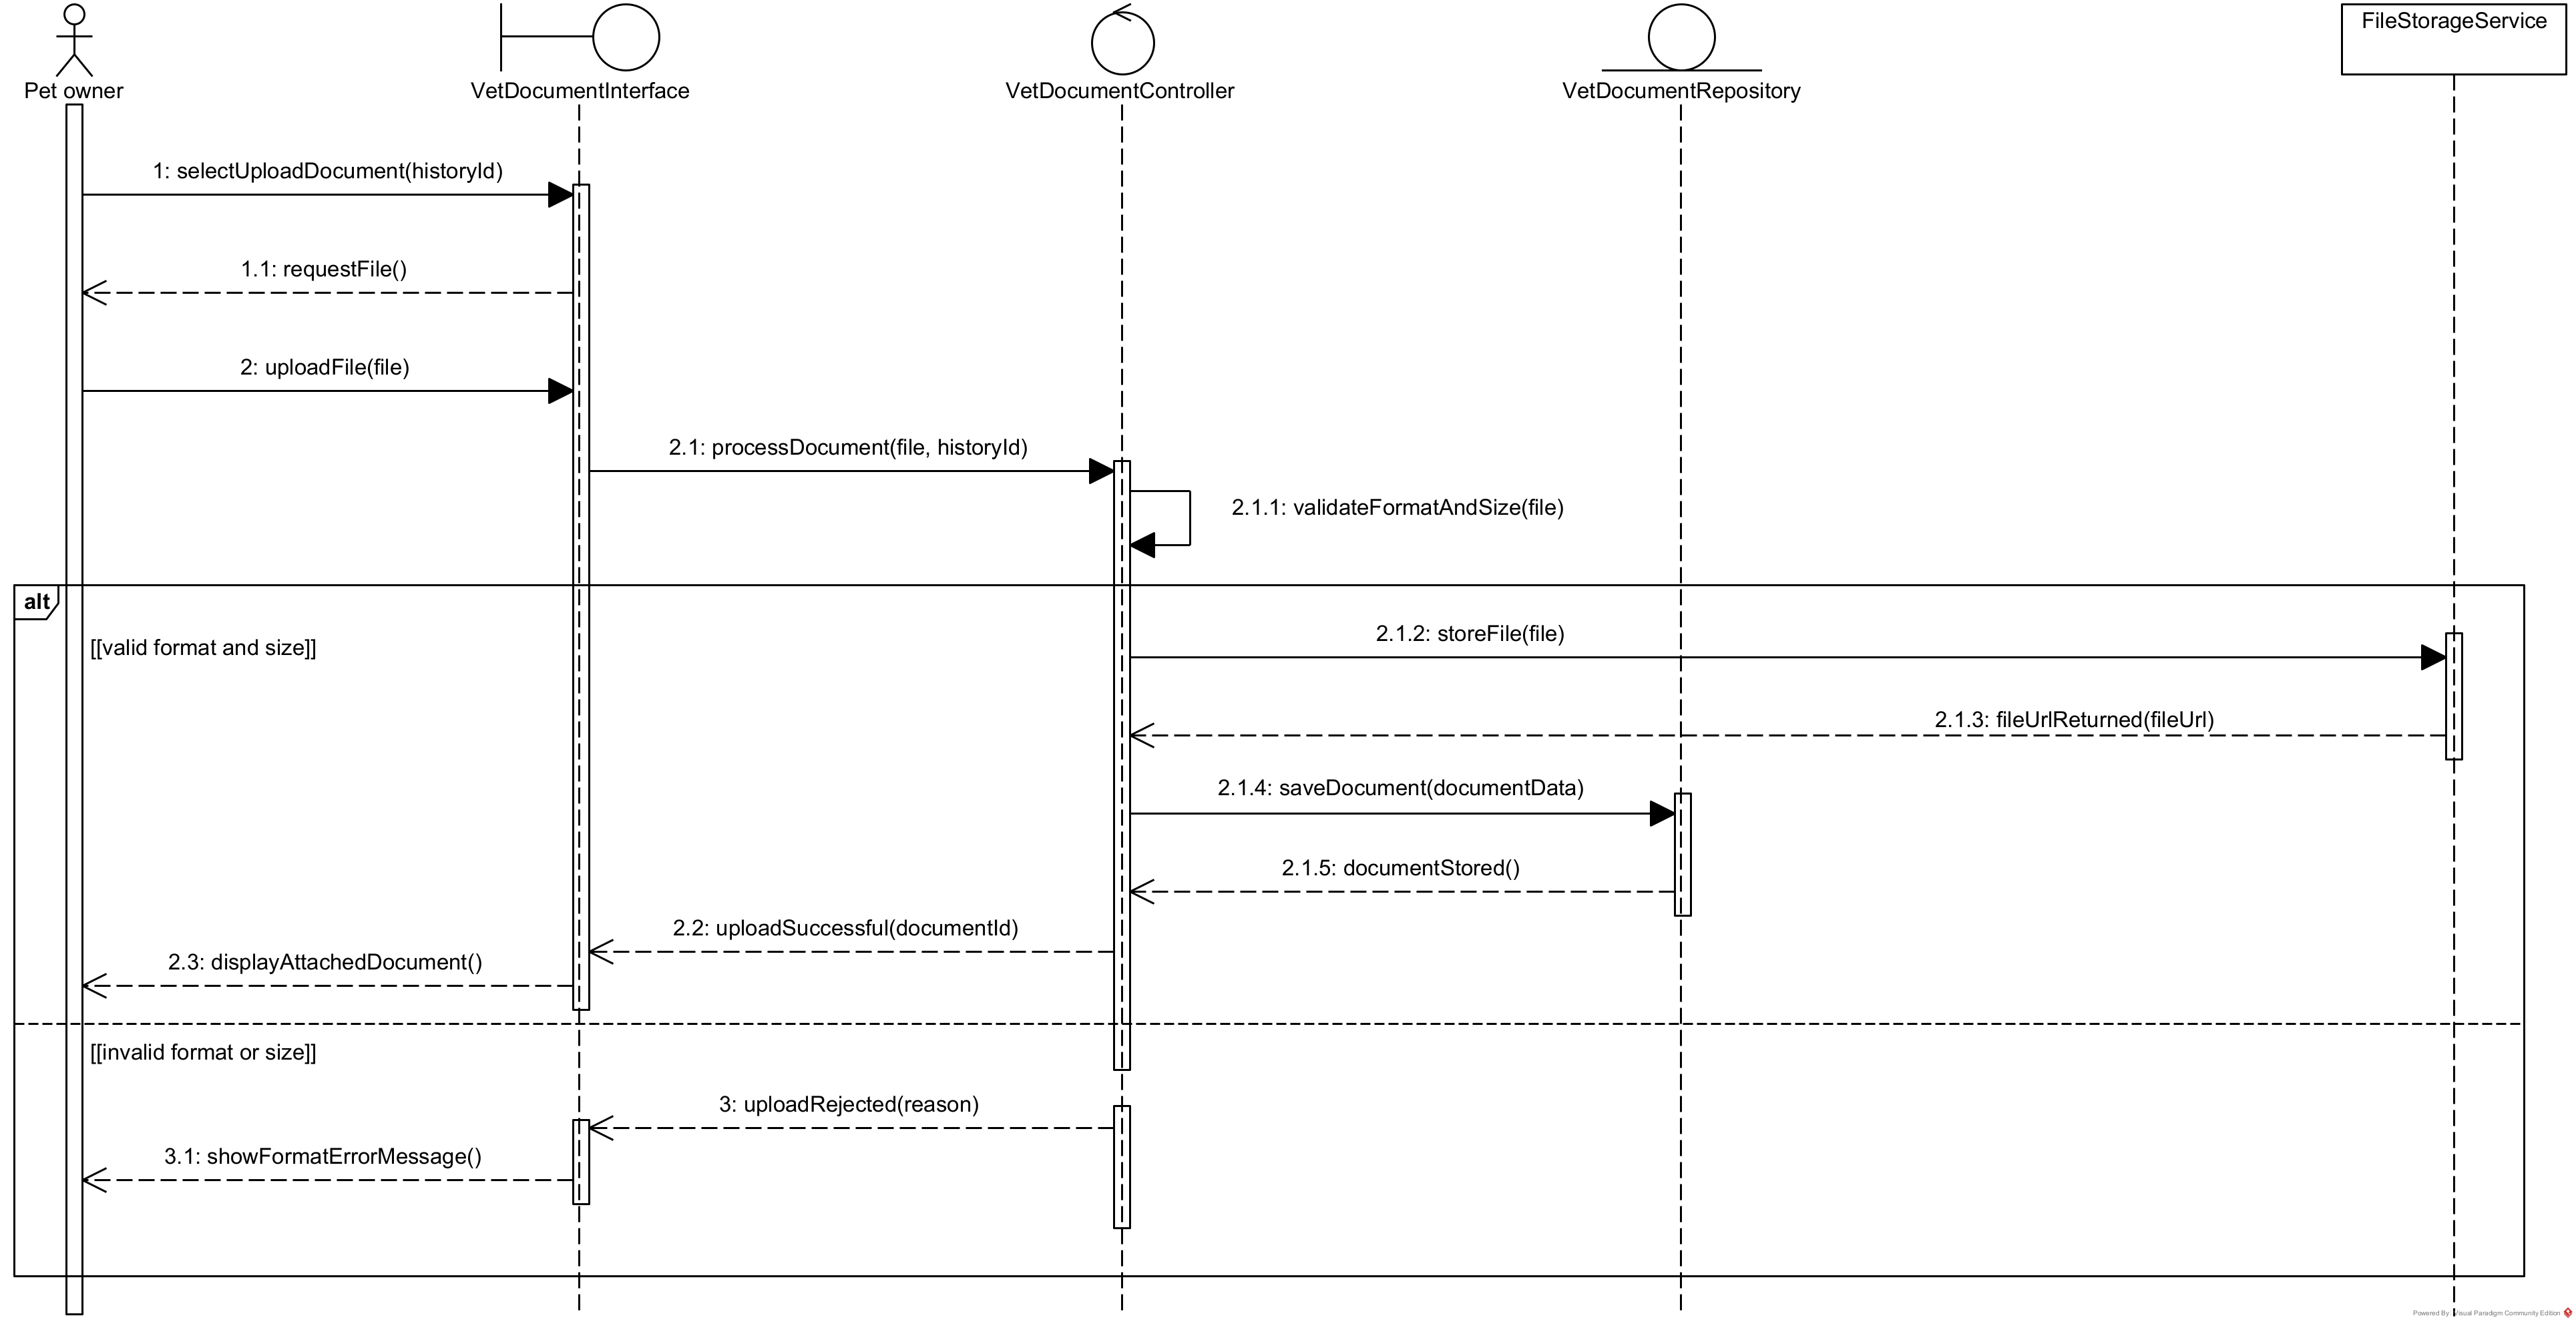
\includegraphics[width=0.72\textwidth]{figuras/DiagramaSecuencia_CU-03_MundiPets.png}
		\caption{Diagrama de secuencia del caso de uso CU-03 --- Cargar documento veterinario y carnet de vacunación.}
		\label{fig:sec-cu03}
	\end{figure}
	
	\subsubsection{Publicar mascota en adopción (CU-04)}
	
	El diagrama de secuencia de CU-04 representa el proceso de publicación
	descrito en RF-13, en el cual el propietario selecciona una mascota ya
	registrada, indica el tipo de disponibilidad (adopción, cruza o ambas) y
	confirma la publicación. Un aspecto relevante de esta secuencia es la
	verificación de completitud del perfil antes de habilitar el botón de
	publicación: si faltan campos relevantes como vacunas o fotografías, el
	sistema muestra una advertencia preventiva en línea con la funcionalidad de
	sugerencias inteligentes descrita en el alcance del producto, sin bloquear
	la publicación de forma definitiva.
	
	\begin{figure}[H]
		\centering
		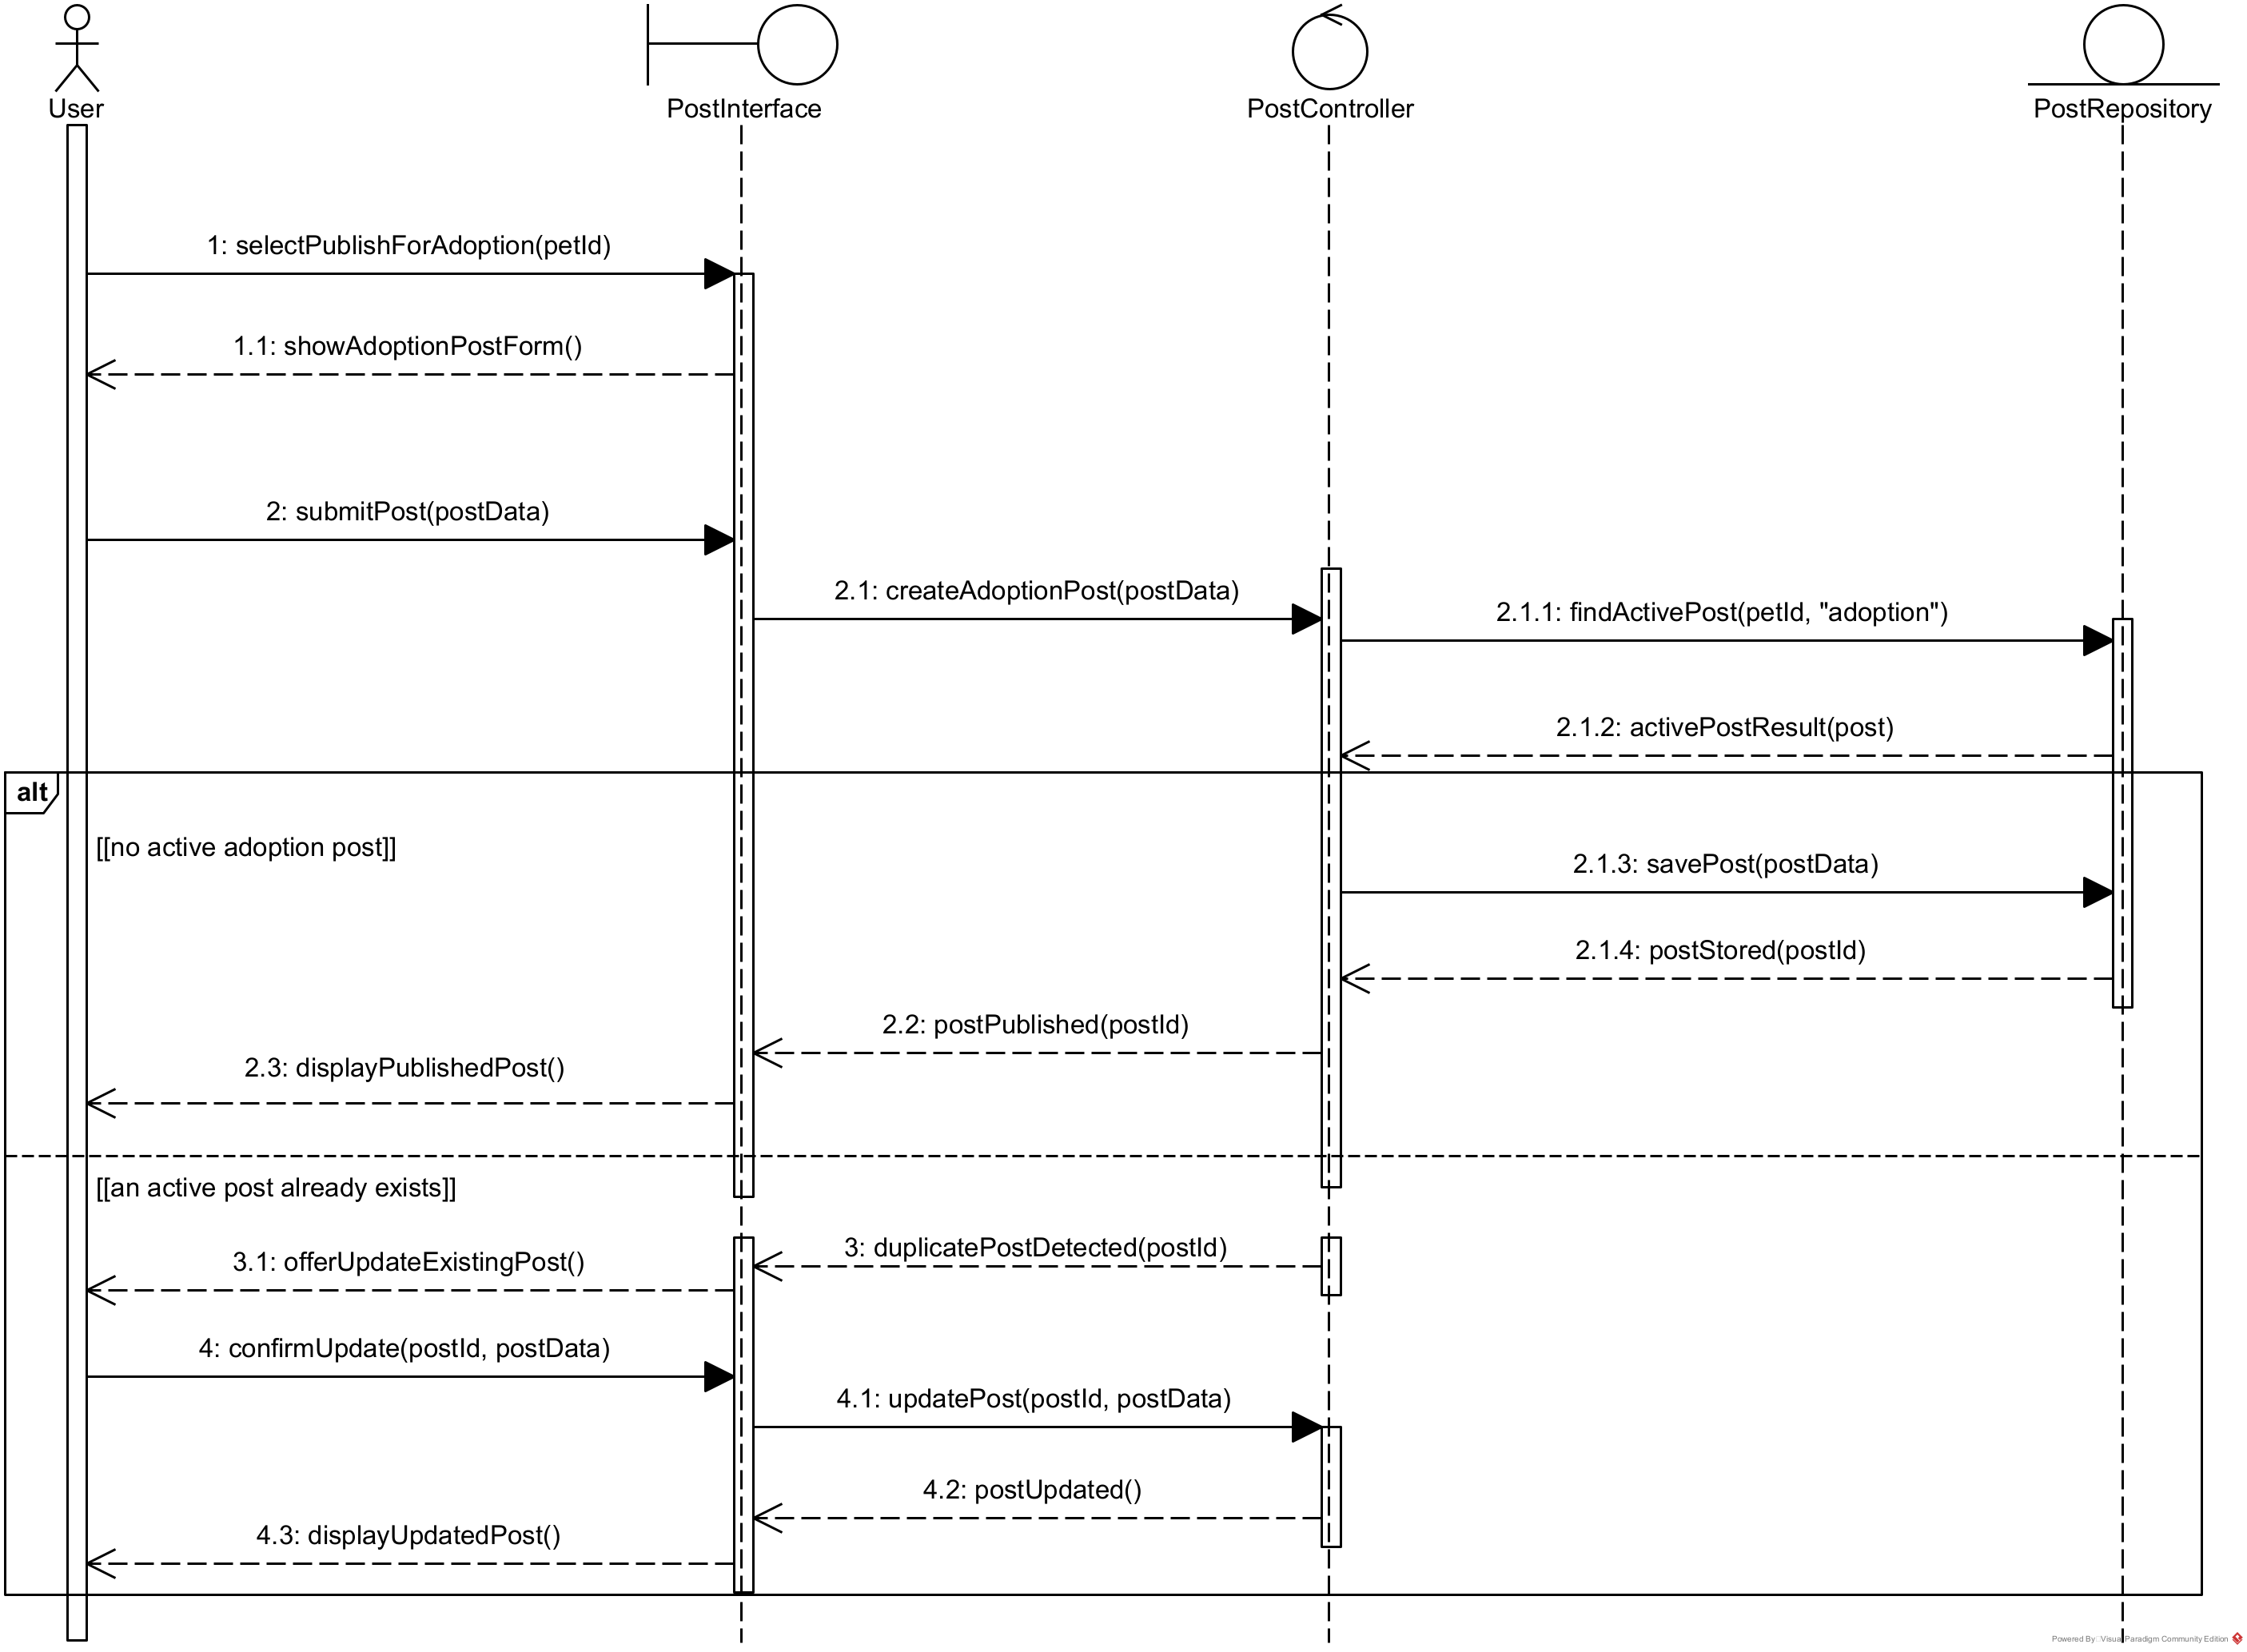
\includegraphics[width=0.72\textwidth]{figuras/DiagramaSecuencia_CU-04_MundiPets.png}
		\caption{Diagrama de secuencia del caso de uso CU-04 --- Publicar mascota en adopción.}
		\label{fig:sec-cu04}
	\end{figure}
	
	\subsubsection{Publicar mascota para cruza y gestionar solicitud (CU-05)}
	
	Esta secuencia cubre la publicación de una mascota disponible para cruza
	responsable y la gestión posterior de la solicitud correspondiente (RF-08,
	RF-13). El diagrama muestra cómo el controlador verifica, antes de habilitar
	la publicación, que la mascota cuente con antecedentes genéticos registrados
	(RF-16); solo entonces la solicitud del interesado en cruza puede avanzar
	hacia el estado pendiente. La respuesta del propietario receptor (aceptar o
	rechazar) se propaga como un mensaje asíncrono de actualización de estado
	hacia el objeto \texttt{SolicitudCruza}, coherente con la máquina de estados
	presentada en la Sección~\ref{sec:estados}.
	
	\begin{figure}[H]
		\centering
		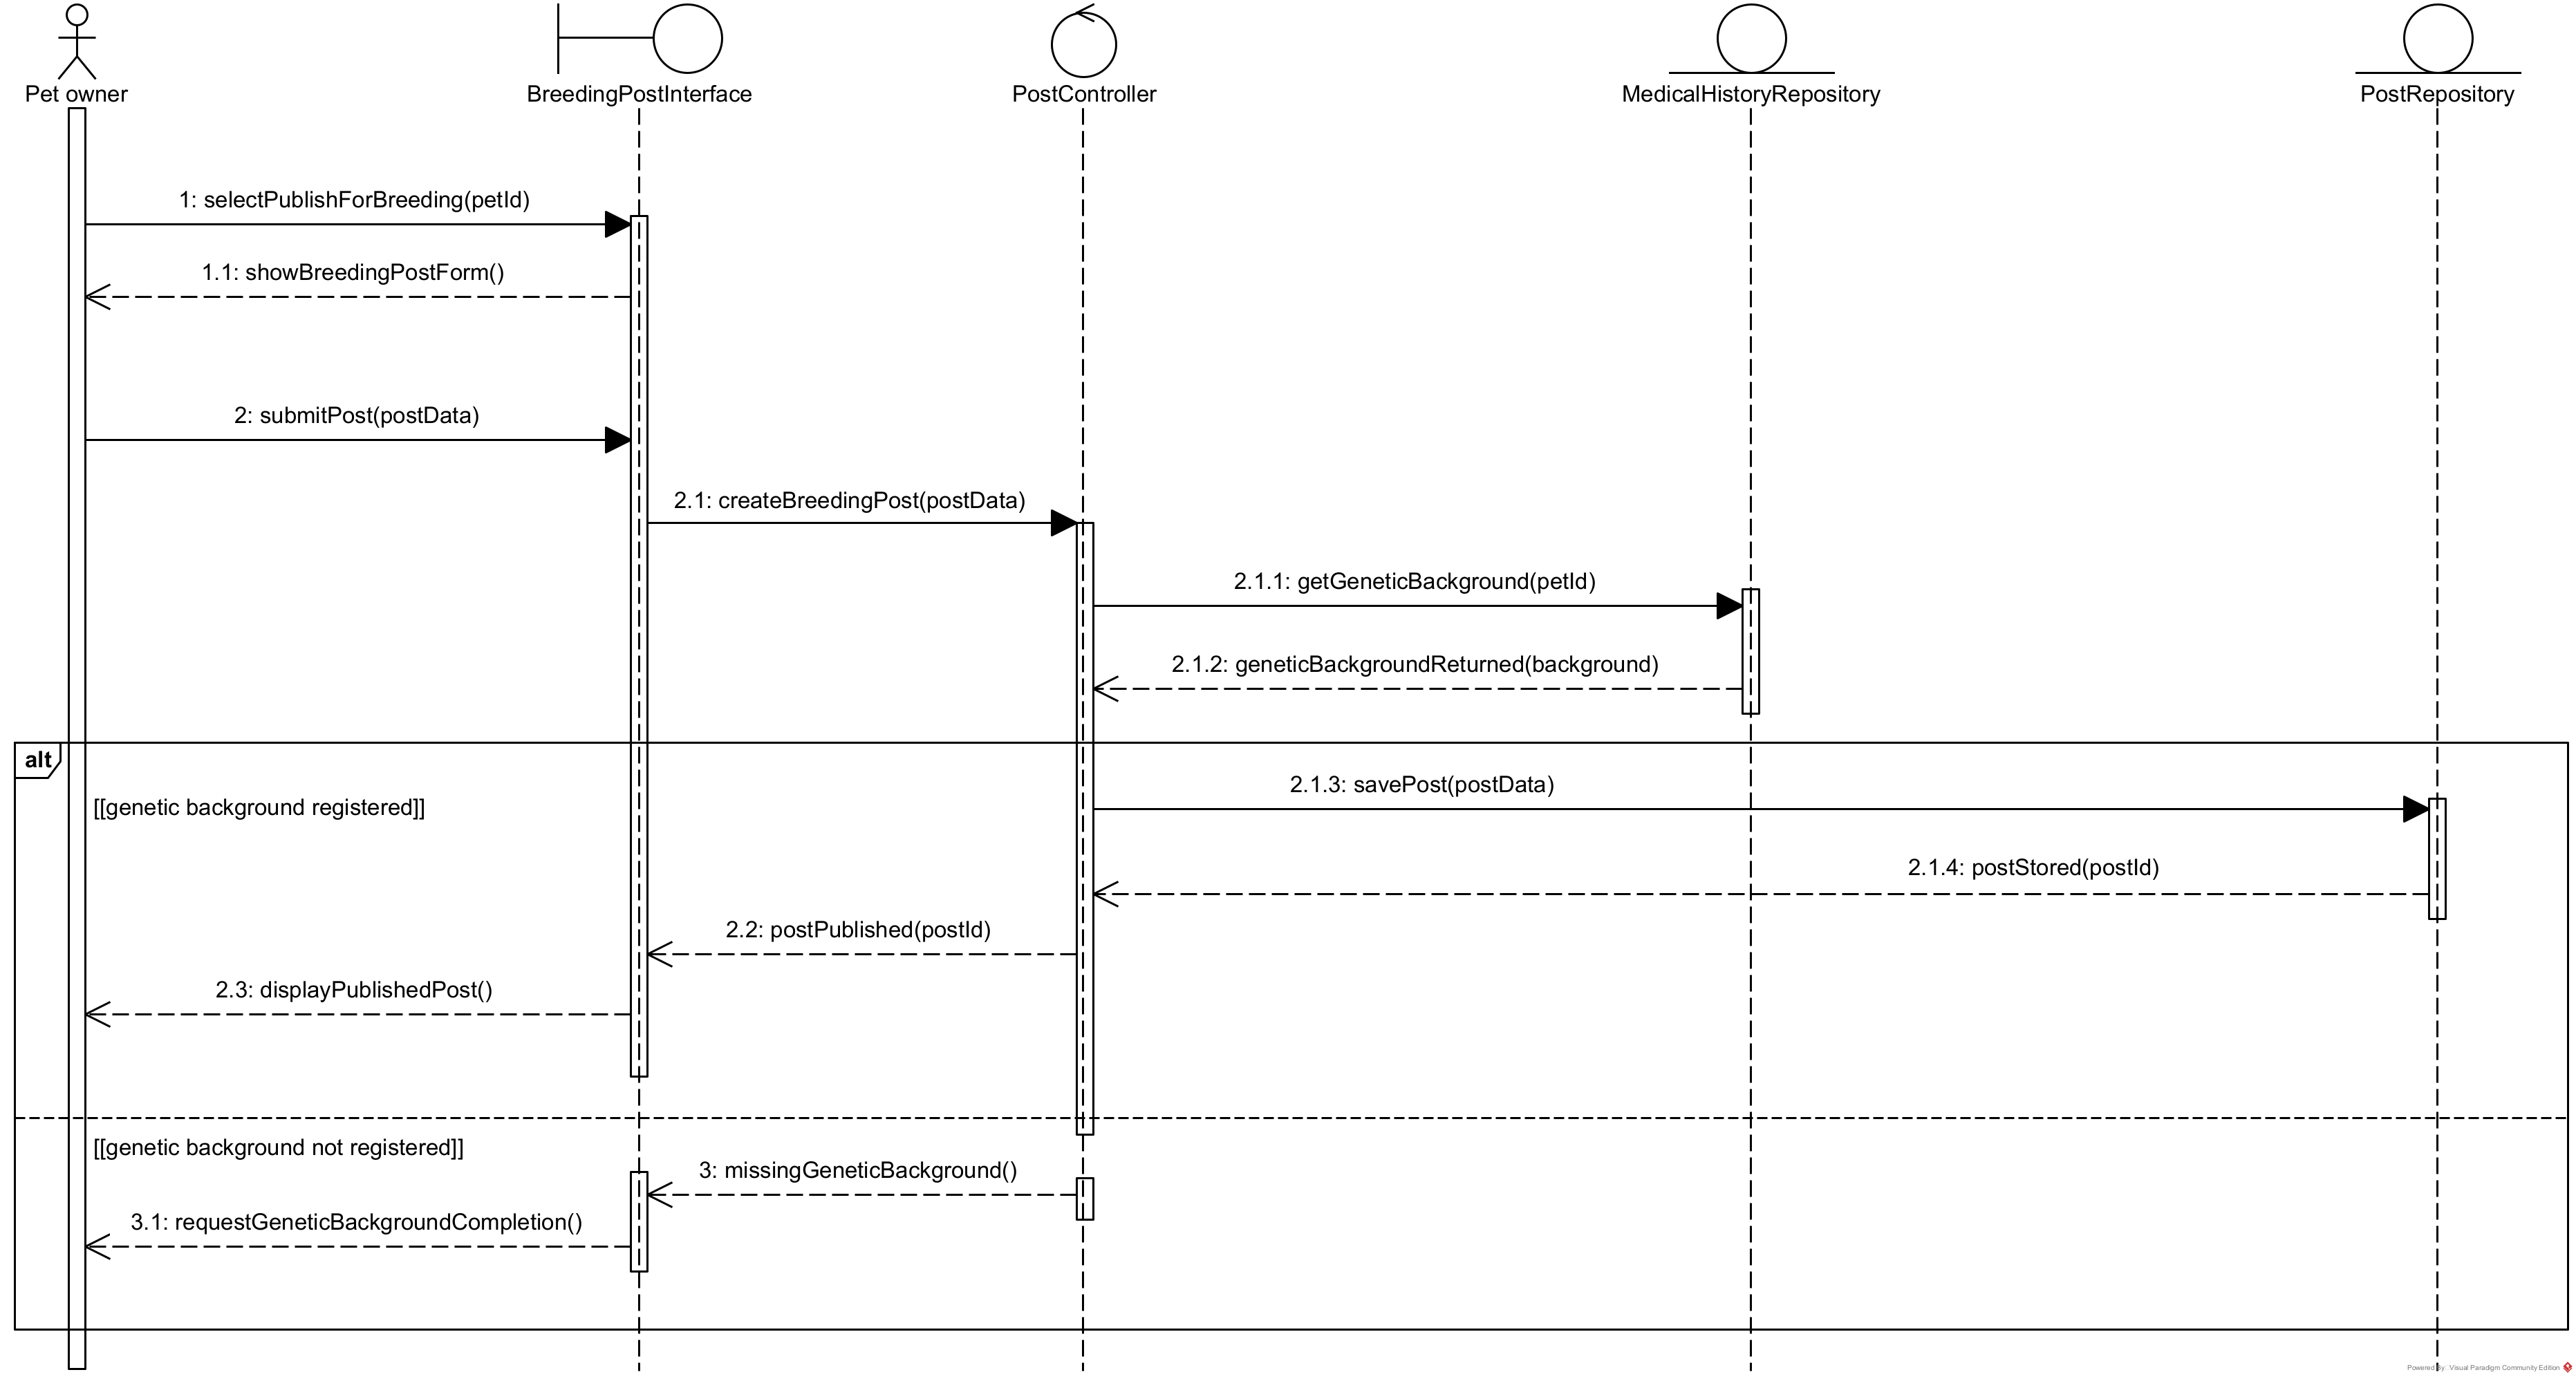
\includegraphics[width=0.72\textwidth]{figuras/DiagramaSecuencia_CU-05_MundiPets.png}
		\caption{Diagrama de secuencia del caso de uso CU-05 --- Publicar mascota para cruza y gestionar solicitud.}
		\label{fig:sec-cu05}
	\end{figure}
	
	\subsubsection{Evaluar compatibilidad de cruza (CU-06)}
	
	Esta secuencia detalla la interacción más compleja del sistema desde el
	punto de vista de la inteligencia artificial. Tras la selección de las dos
	mascotas por parte del usuario, el controlador reúne los antecedentes
	genéticos, el historial médico y los datos generales de ambas y los envía al
	componente de evaluación de compatibilidad (RF-06). El diagrama muestra de
	forma explícita la generación de la explicación causal exigida por RNF-13,
	la cual se calcula en paralelo al resultado numérico y se adjunta a la
	respuesta antes de que esta llegue a la interfaz, cumpliendo el límite de
	dos segundos establecido en dicho requisito no funcional.
	
	\begin{figure}[H]
		\centering
		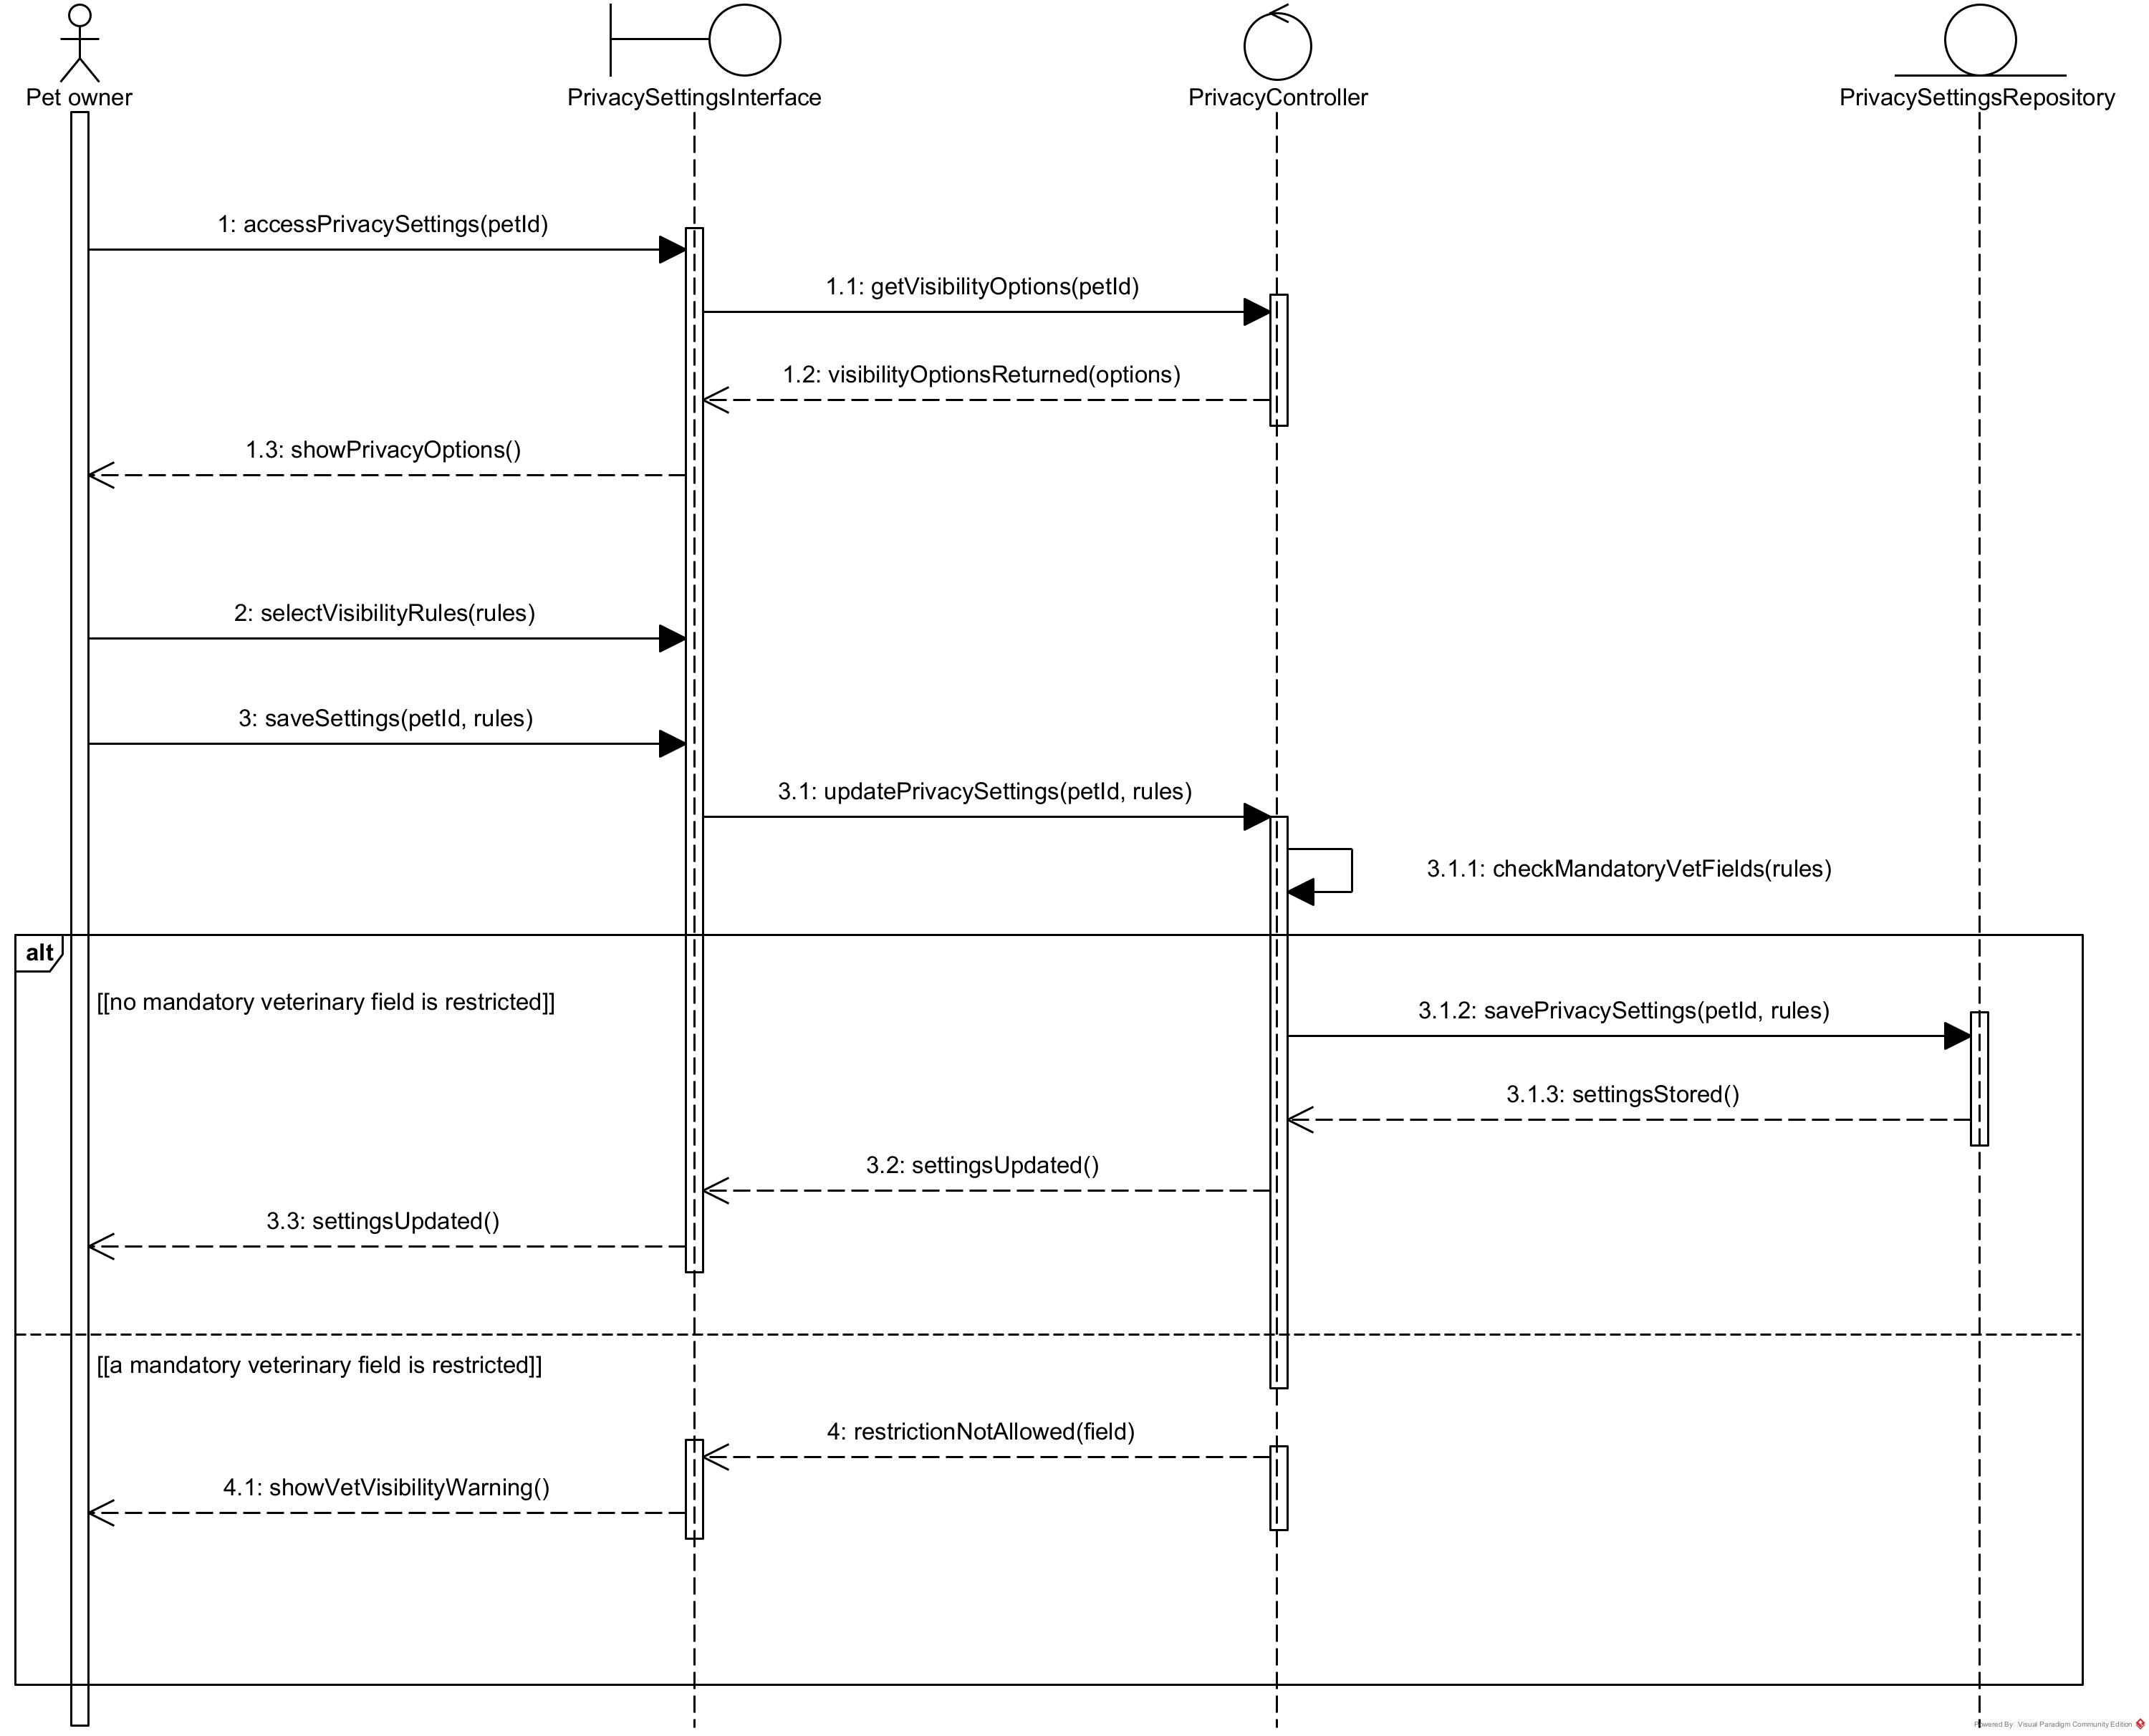
\includegraphics[width=0.72\textwidth]{figuras/DiagramaSecuencia_CU-06_MundiPets.png}
		\caption{Diagrama de secuencia del caso de uso CU-06 --- Evaluar compatibilidad de cruza.}
		\label{fig:sec-cu06}
	\end{figure}
	
	\subsubsection{Consultar historial de procesos de adopción y cruza (CU-07)}
	
	El diagrama de secuencia de CU-07 modela la consulta que realiza el
	propietario sobre el historial de solicitudes asociadas a sus mascotas
	(RF-15). El controlador recupera de forma paralela las solicitudes de
	adopción y de cruza registradas, las combina en una única línea de tiempo
	ordenada por fecha y las retorna a la interfaz junto con el estado vigente
	de cada una, sin exponer datos de contacto de los solicitantes que no hayan
	sido aceptados, en cumplimiento del principio de minimización de datos
	descrito en RL-05.
	
	\begin{figure}[H]
		\centering
		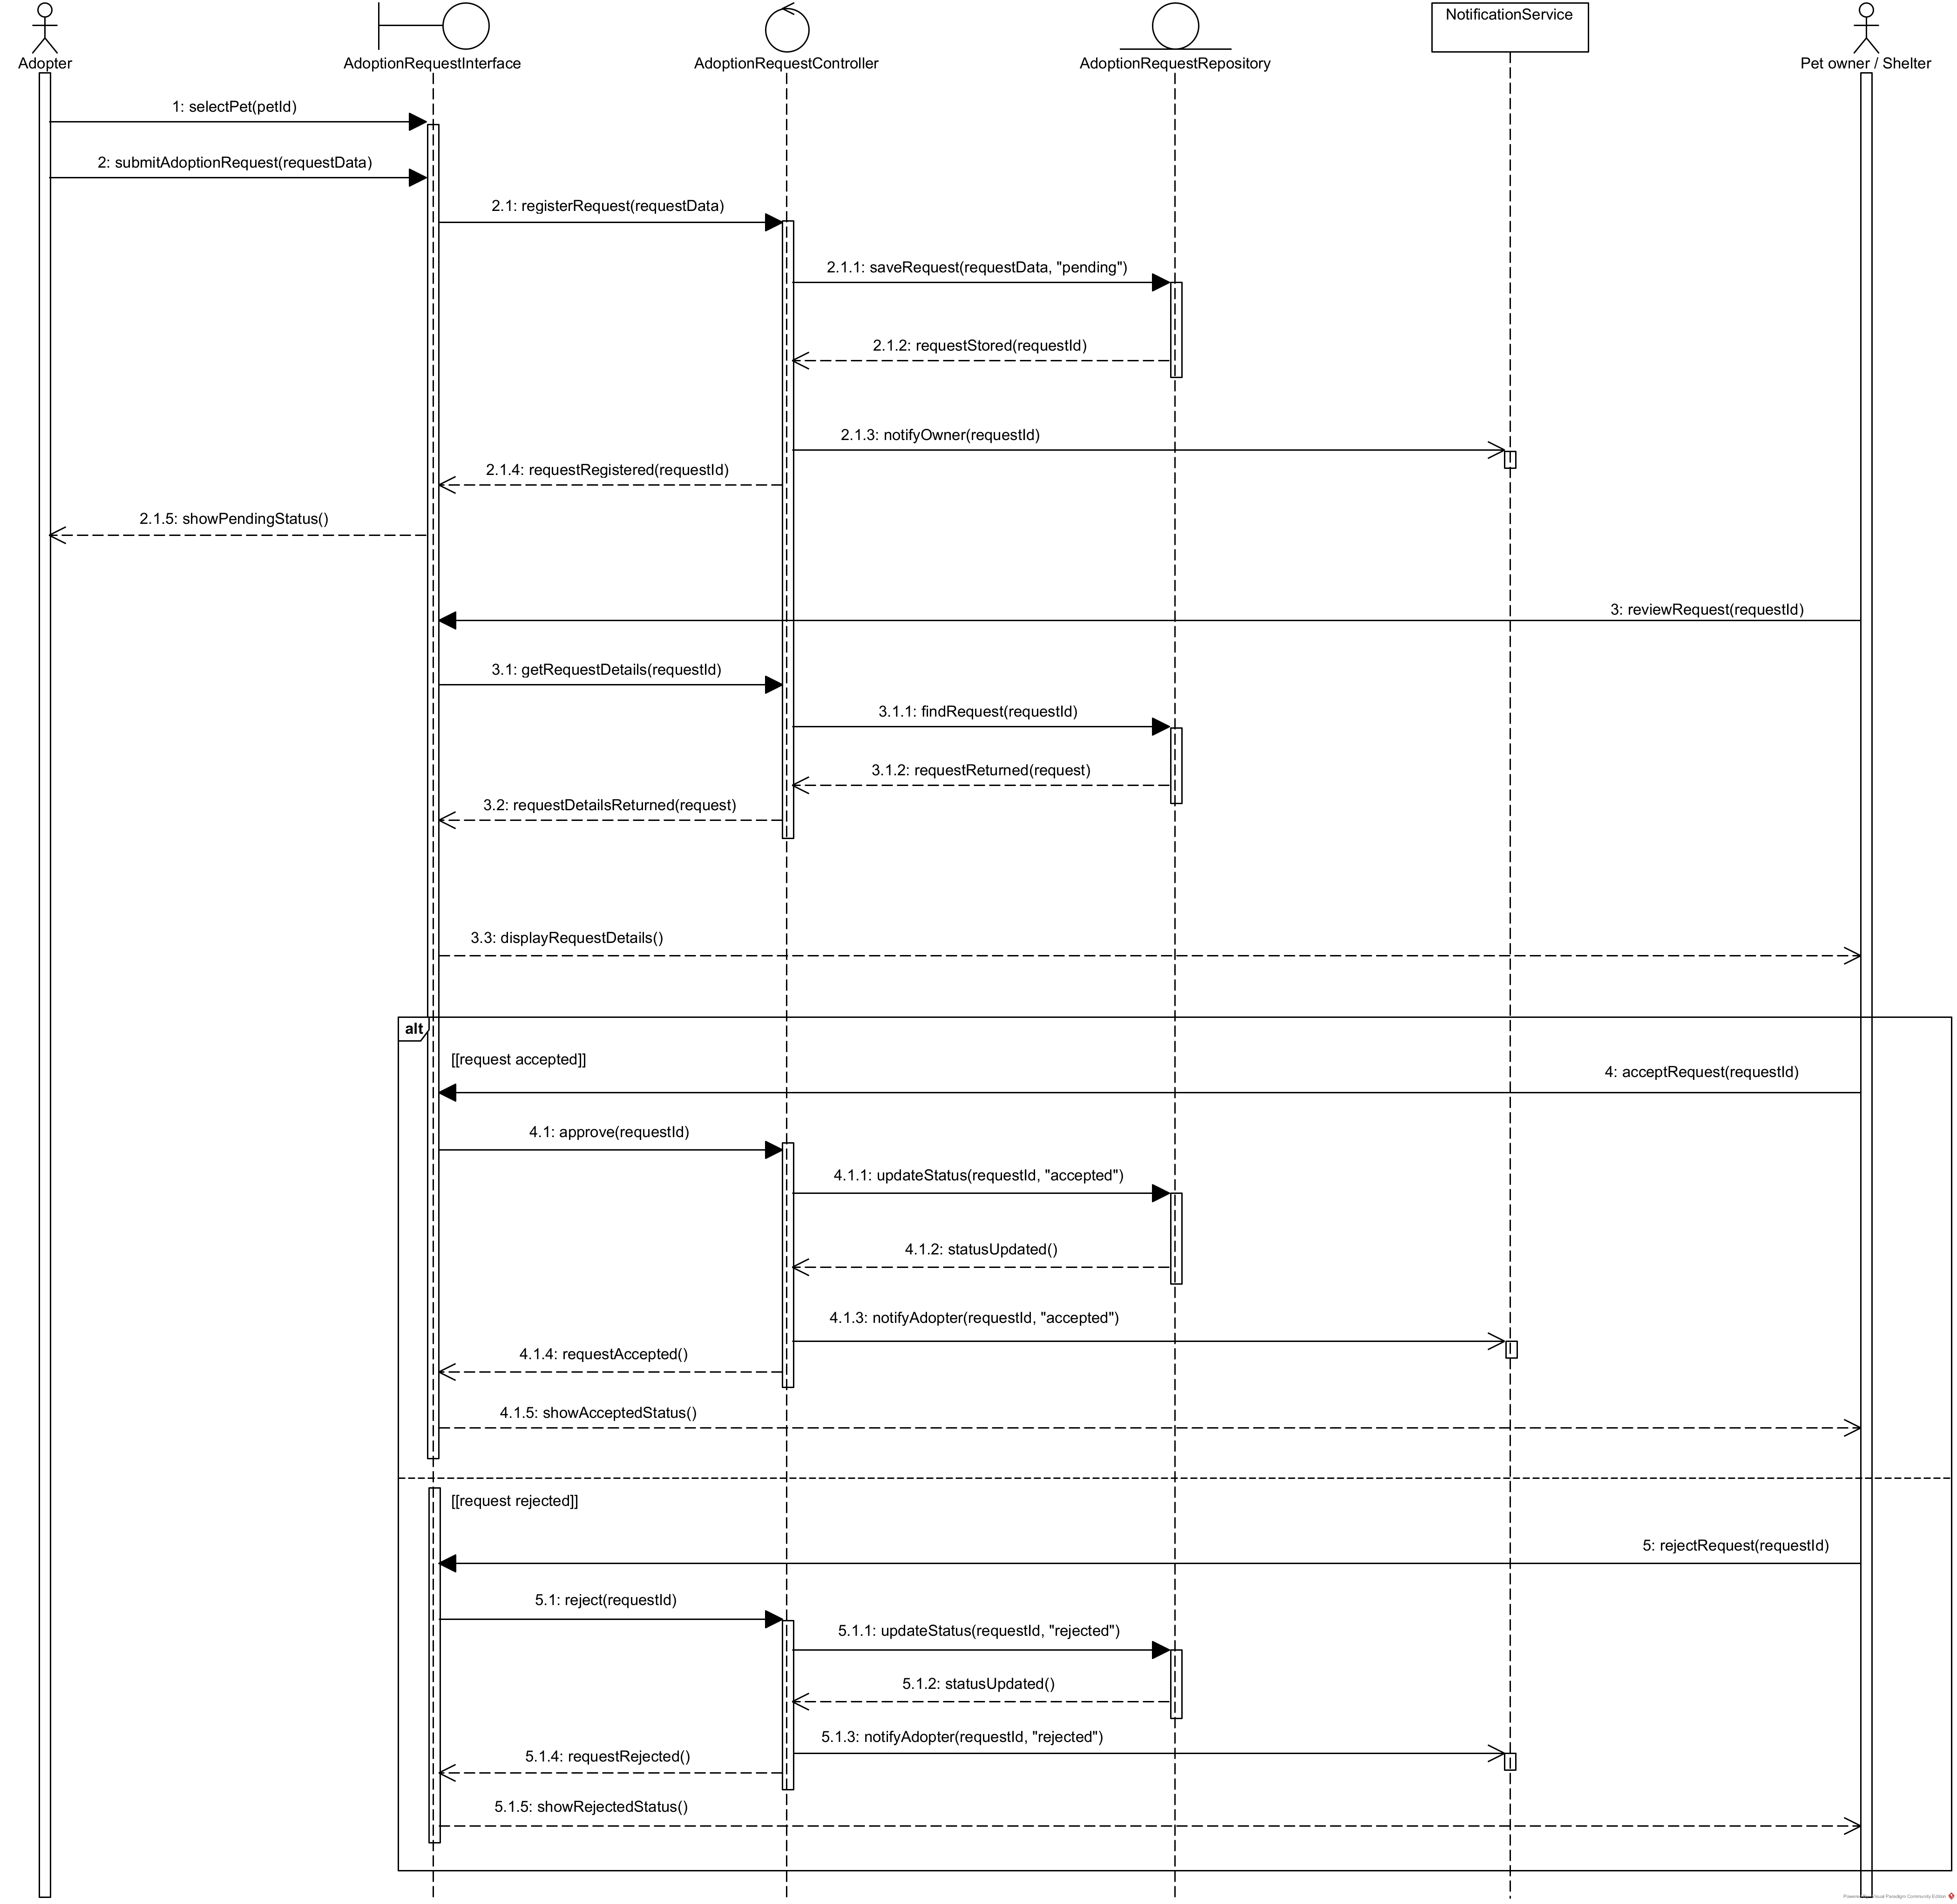
\includegraphics[width=0.72\textwidth]{figuras/DiagramaSecuencia_CU-07_MundiPets.png}
		\caption{Diagrama de secuencia del caso de uso CU-07 --- Consultar historial de procesos de adopción y cruza.}
		\label{fig:sec-cu07}
	\end{figure}
	
	\subsubsection{Gestionar comunicación entre usuarios (CU-08)}
	
	Esta secuencia representa el intercambio de mensajes entre propietario,
	adoptante e interesado en cruza (RF-07). Cada mensaje enviado pasa primero
	por el componente de moderación automática antes de almacenarse; si el
	contenido es marcado como inapropiado, la secuencia se bifurca hacia el
	flujo de bloqueo, que notifica al remitente la categoría de infracción
	detectada conforme a la explicación por ejemplos exigida por RNF-15, sin
	llegar a entregar el mensaje al destinatario. Solo los mensajes que superan
	la moderación se persisten y se notifican al receptor.
	
	\begin{figure}[H]
		\centering
		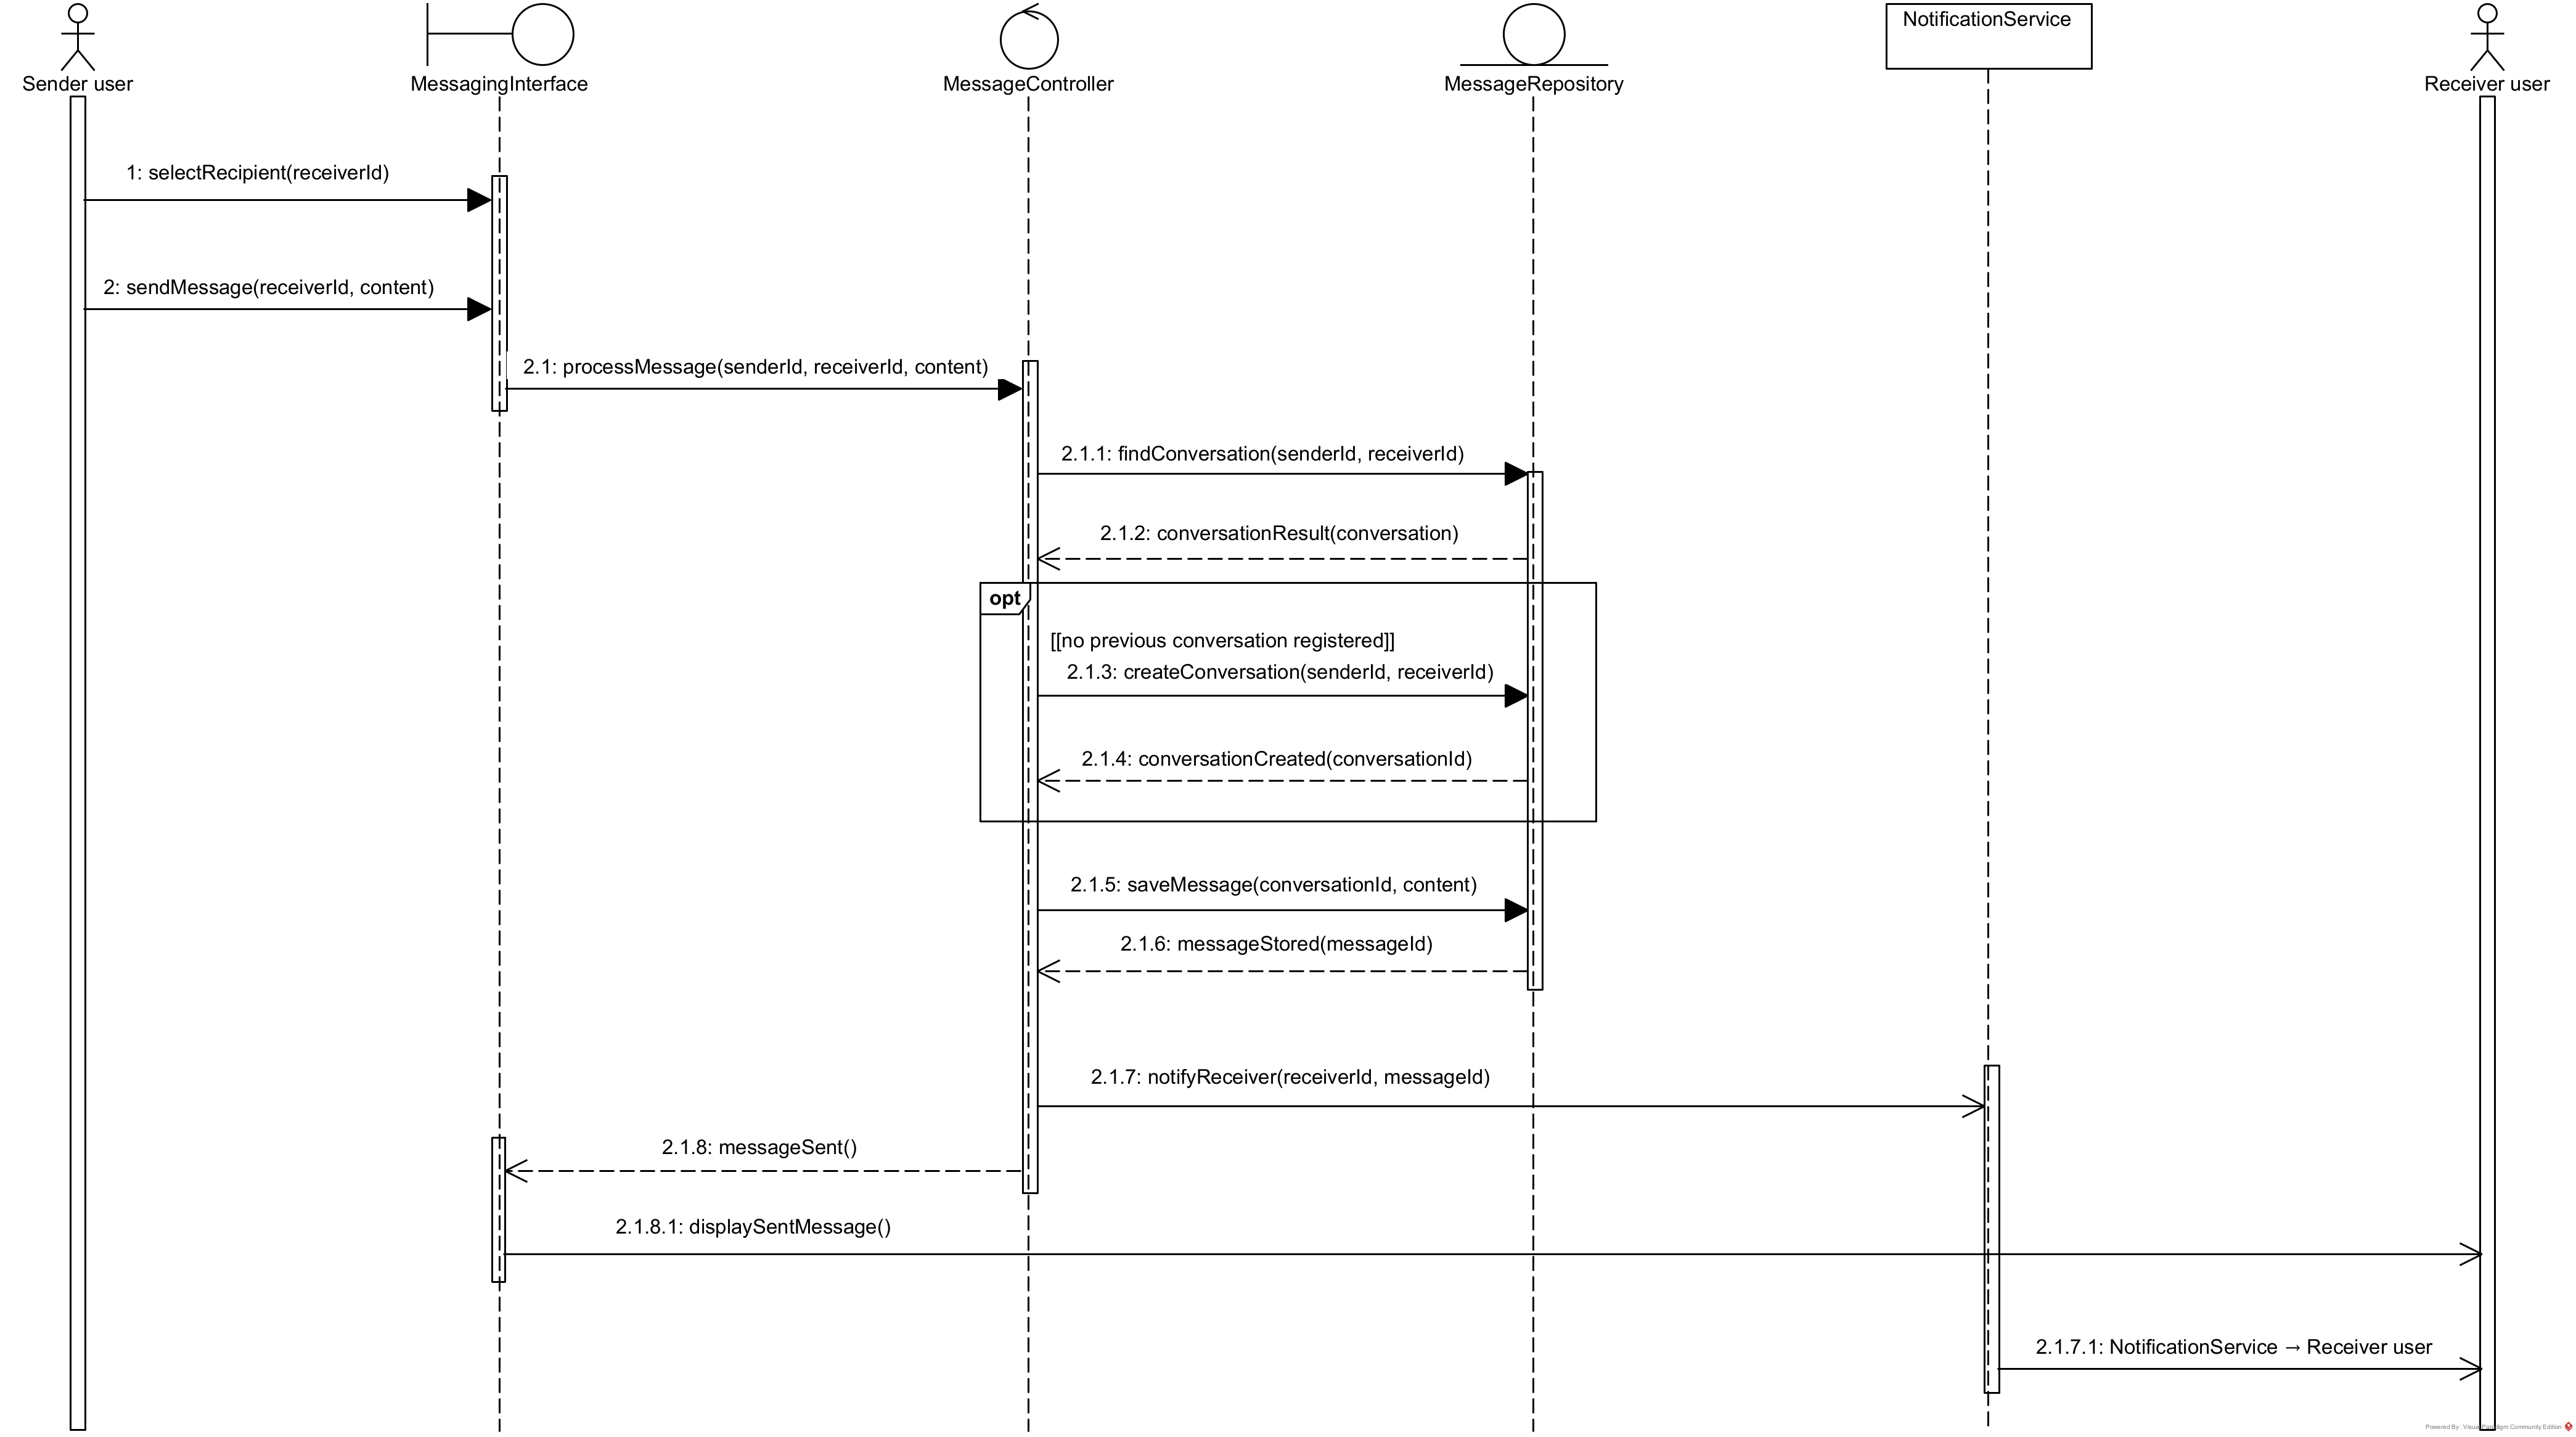
\includegraphics[width=0.72\textwidth]{figuras/DiagramaSecuencia_CU-08_MundiPets.png}
		\caption{Diagrama de secuencia del caso de uso CU-08 --- Gestionar comunicación entre usuarios.}
		\label{fig:sec-cu08}
	\end{figure}
	
	\subsubsection{Validar información médica (CU-09)}
	
	El diagrama de secuencia de CU-09 modela la revisión que realiza la
	veterinaria sobre el historial médico y los documentos cargados por el
	propietario (RF-09). La interacción distingue dos caminos alternos: la
	validación exitosa, que marca la información con el estado validado y la
	identificación del profesional responsable; y el rechazo, que exige a la
	veterinaria registrar una observación técnica antes de poder confirmar la
	operación, evitando rechazos sin justificación que dificulten la
	trazabilidad exigida por el marco legal de la
	Sección~\ref{sec:legales}.
	
	\begin{figure}[H]
		\centering
		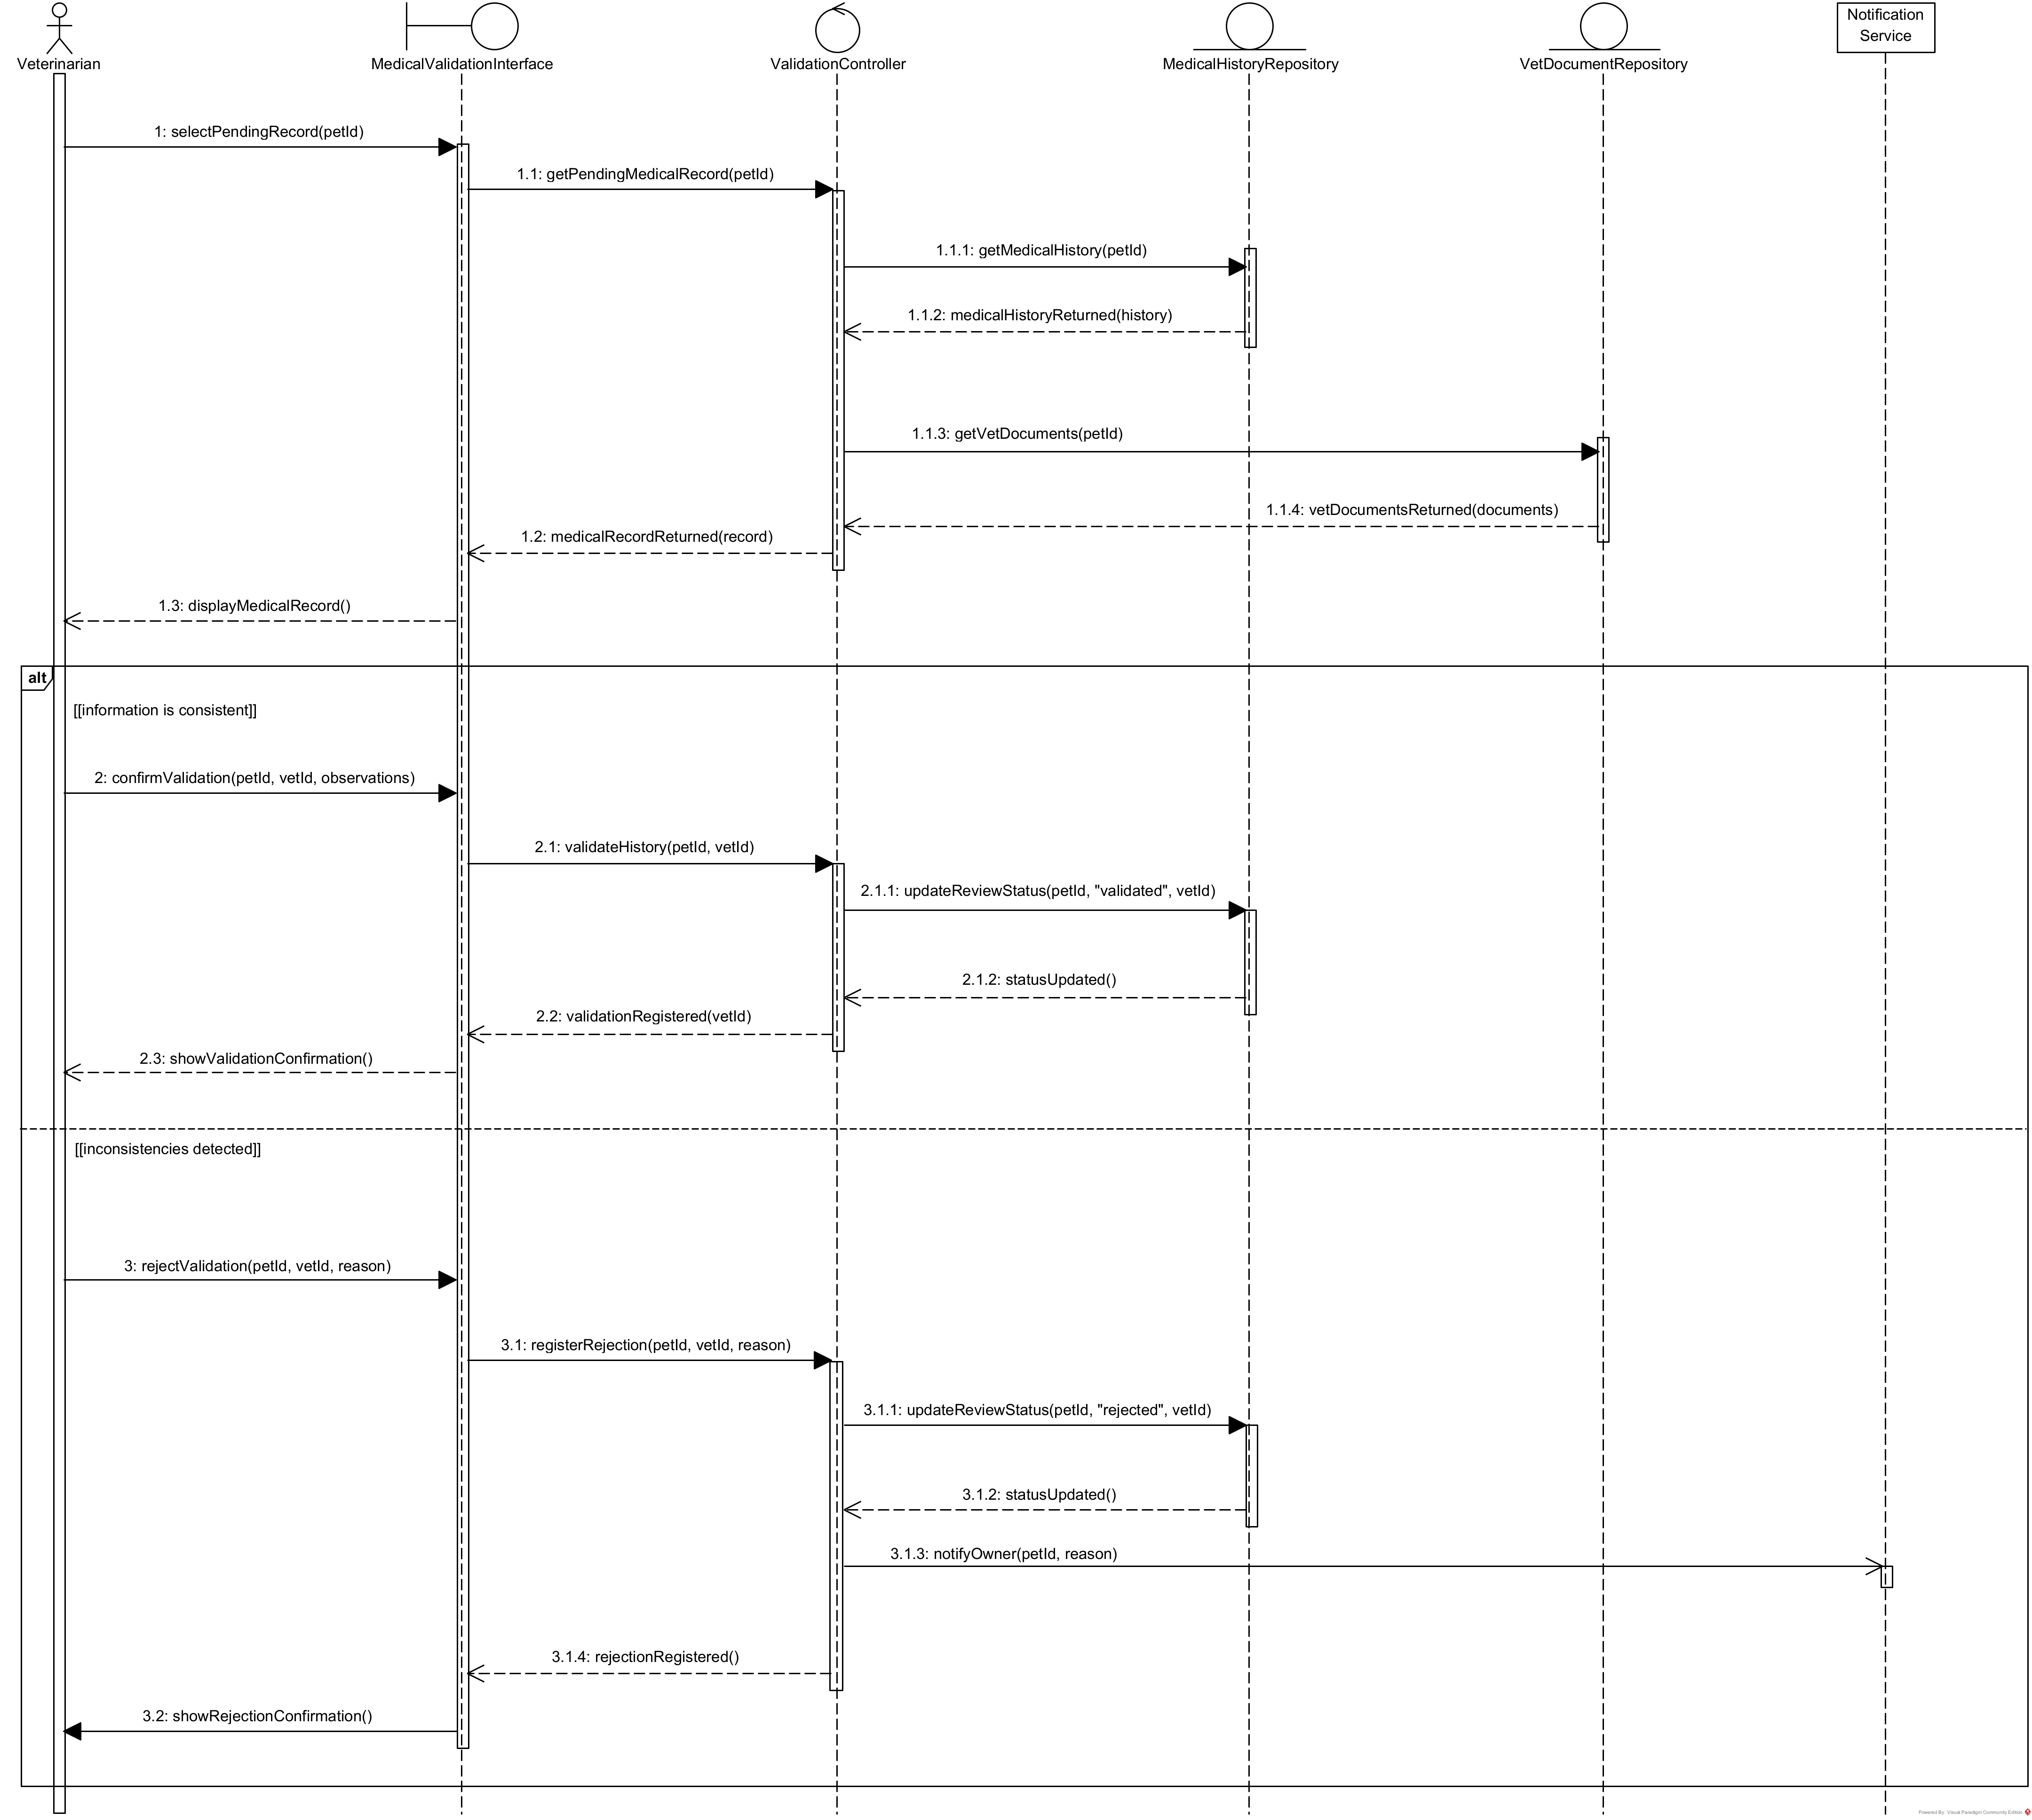
\includegraphics[width=0.72\textwidth]{figuras/DiagramaSecuencia_CU-09_MundiPets.png}
		\caption{Diagrama de secuencia del caso de uso CU-09 --- Validar información médica.}
		\label{fig:sec-cu09}
	\end{figure}
	
	\subsubsection{Consultar perfil médico (CU-10)}
	
	Esta secuencia detalla la consulta de perfil completo de una mascota
	(RF-03), incluyendo la aplicación de las reglas de privacidad configuradas
	por el propietario (RF-11). El controlador determina, antes de retornar la
	información, cuál es el nivel de acceso del usuario consultante
	(propietario, adoptante, interesado en cruza o veterinaria) y filtra en
	consecuencia los campos de ubicación exacta y contacto directo, mostrando
	únicamente la zona aproximada por defecto conforme a RNF-16.
	
	\begin{figure}[H]
		\centering
		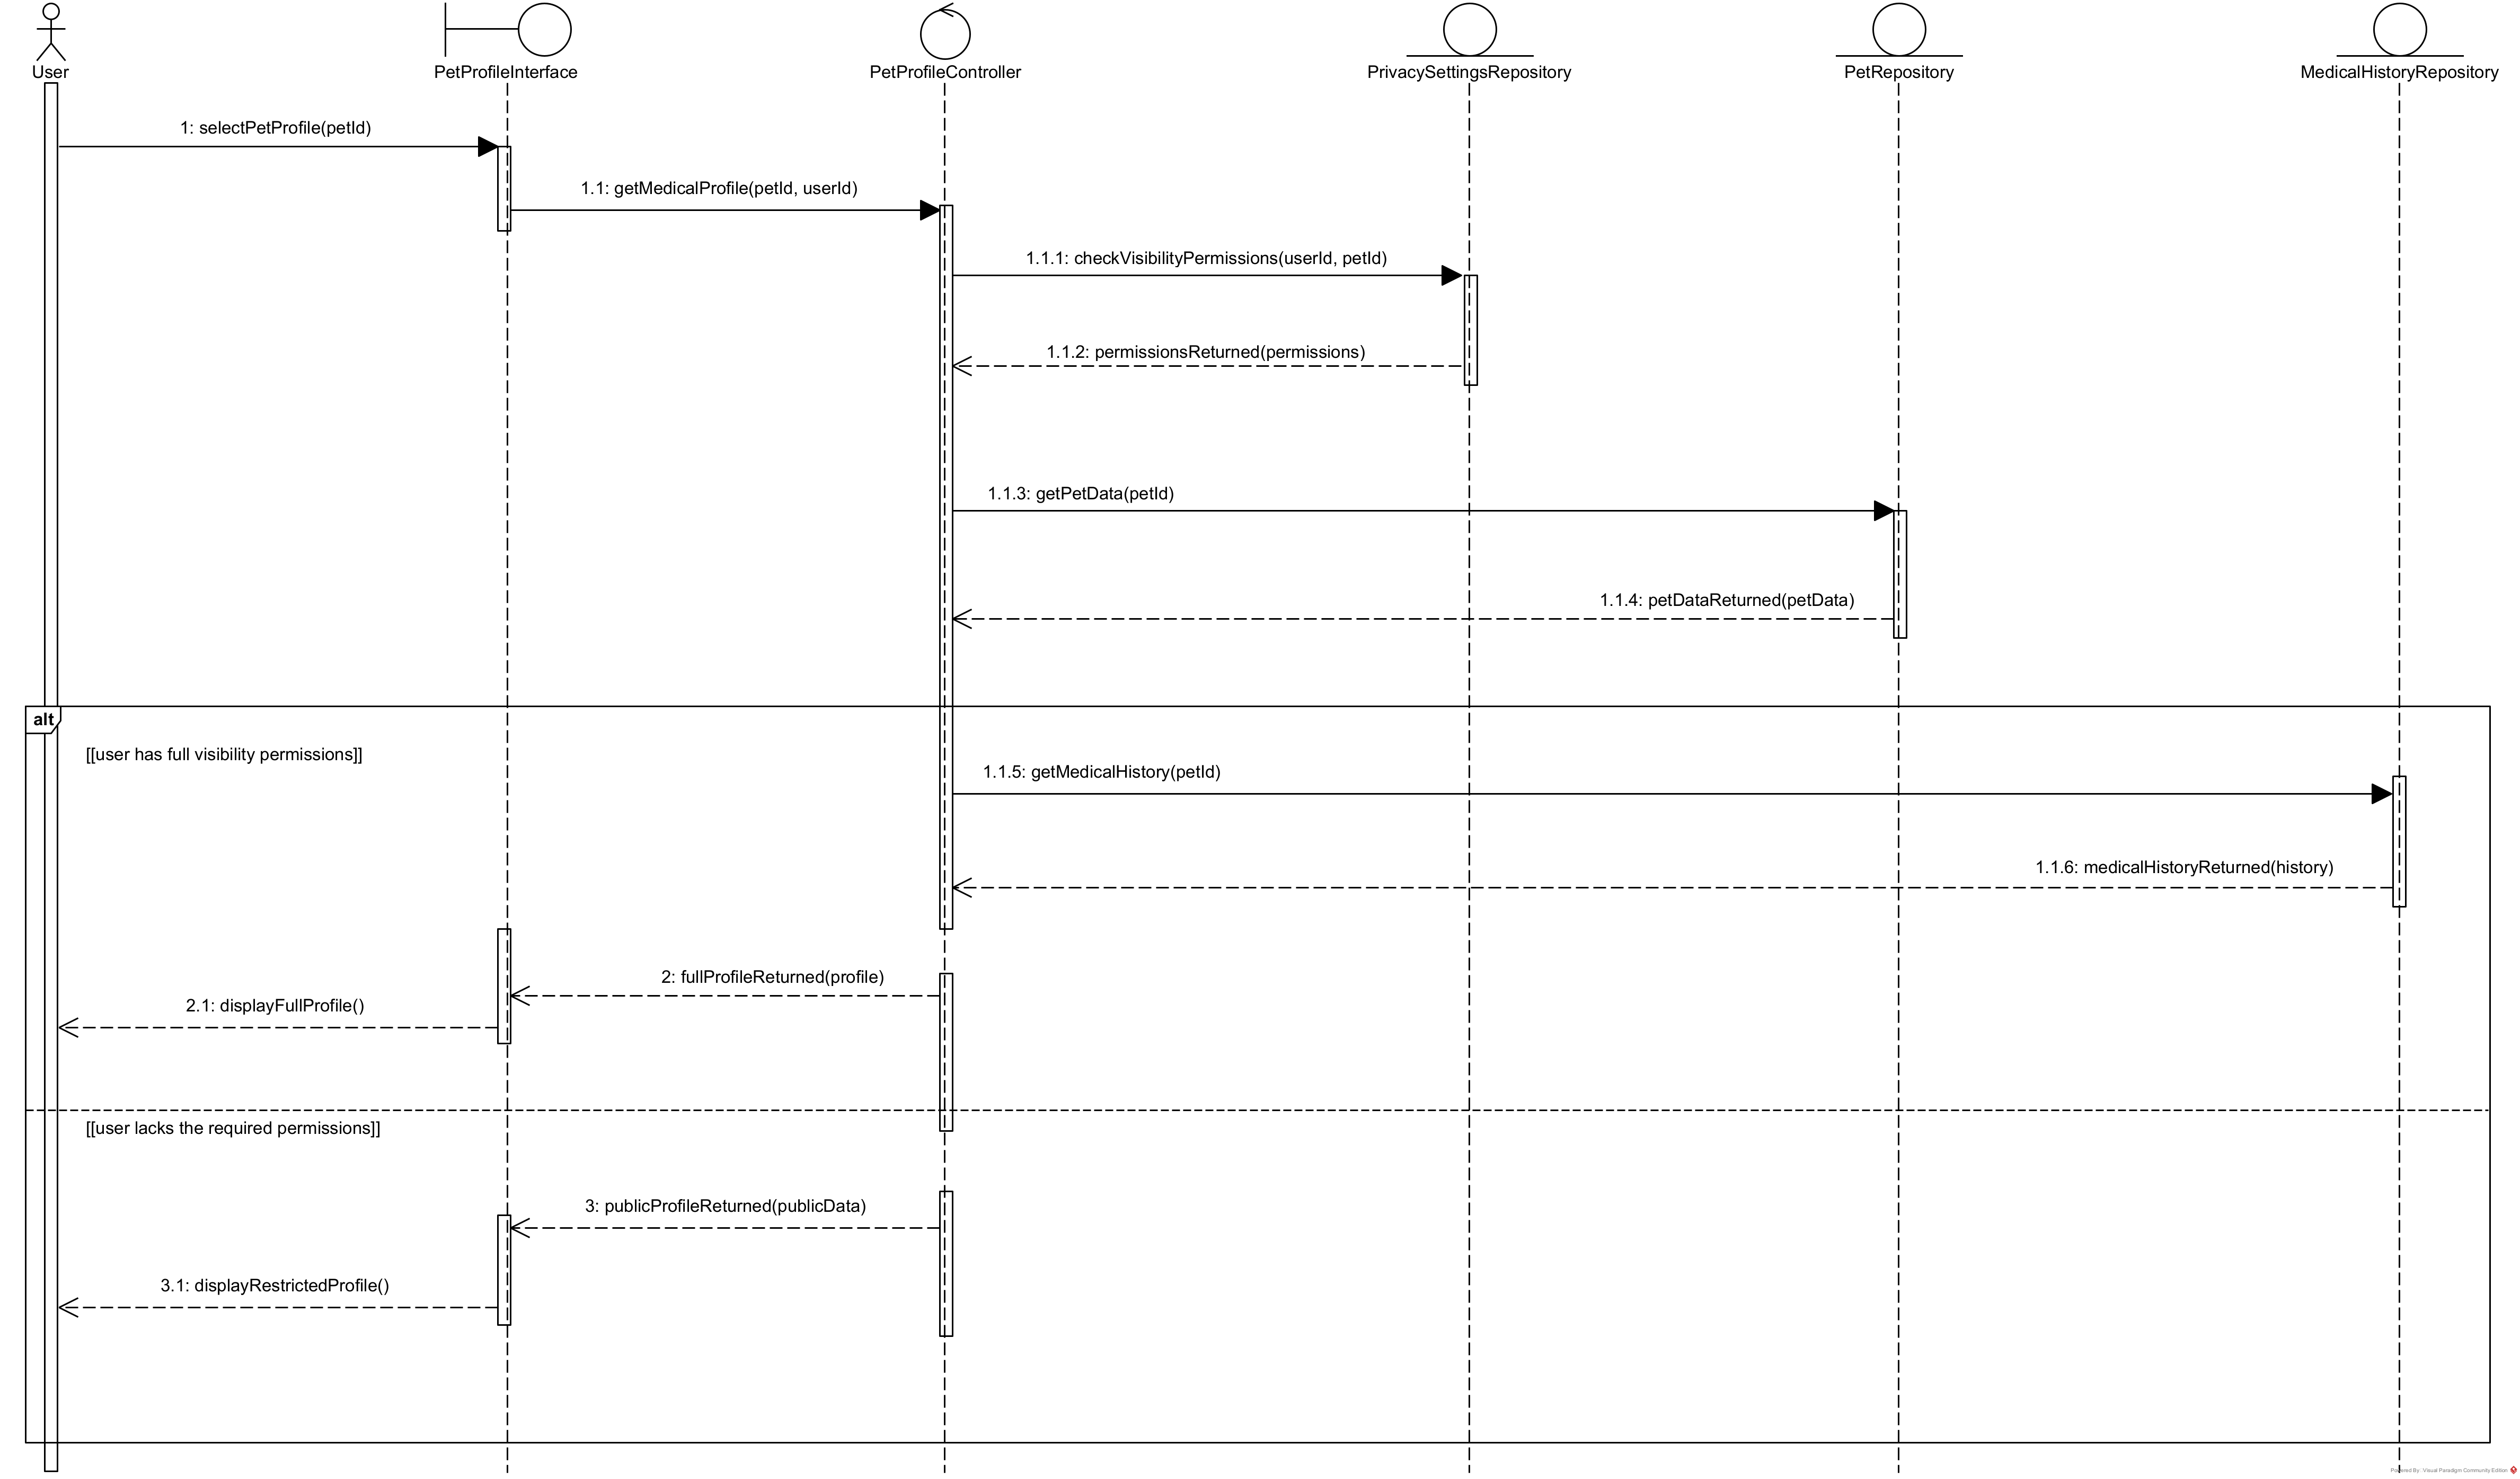
\includegraphics[width=0.72\textwidth]{figuras/DiagramaSecuencia_CU-10_MundiPets.png}
		\caption{Diagrama de secuencia del caso de uso CU-10 --- Consultar perfil médico.}
		\label{fig:sec-cu10}
	\end{figure}
	
	\subsubsection{Buscar mascota disponible (CU-11)}
	
	El diagrama de secuencia de CU-11 modela la búsqueda y el filtrado de
	mascotas disponibles (RF-04). El actor envía los criterios de búsqueda
	(especie, raza, edad, ubicación aproximada, tamaño, temperamento y
	disponibilidad) a la interfaz, que los transmite al controlador; este
	consulta el repositorio de publicaciones activas y retorna únicamente los
	resultados que cumplen simultáneamente todos los filtros aplicados,
	ordenados por relevancia o cercanía según la configuración vigente del
	sistema.
	
	\begin{figure}[H]
		\centering
		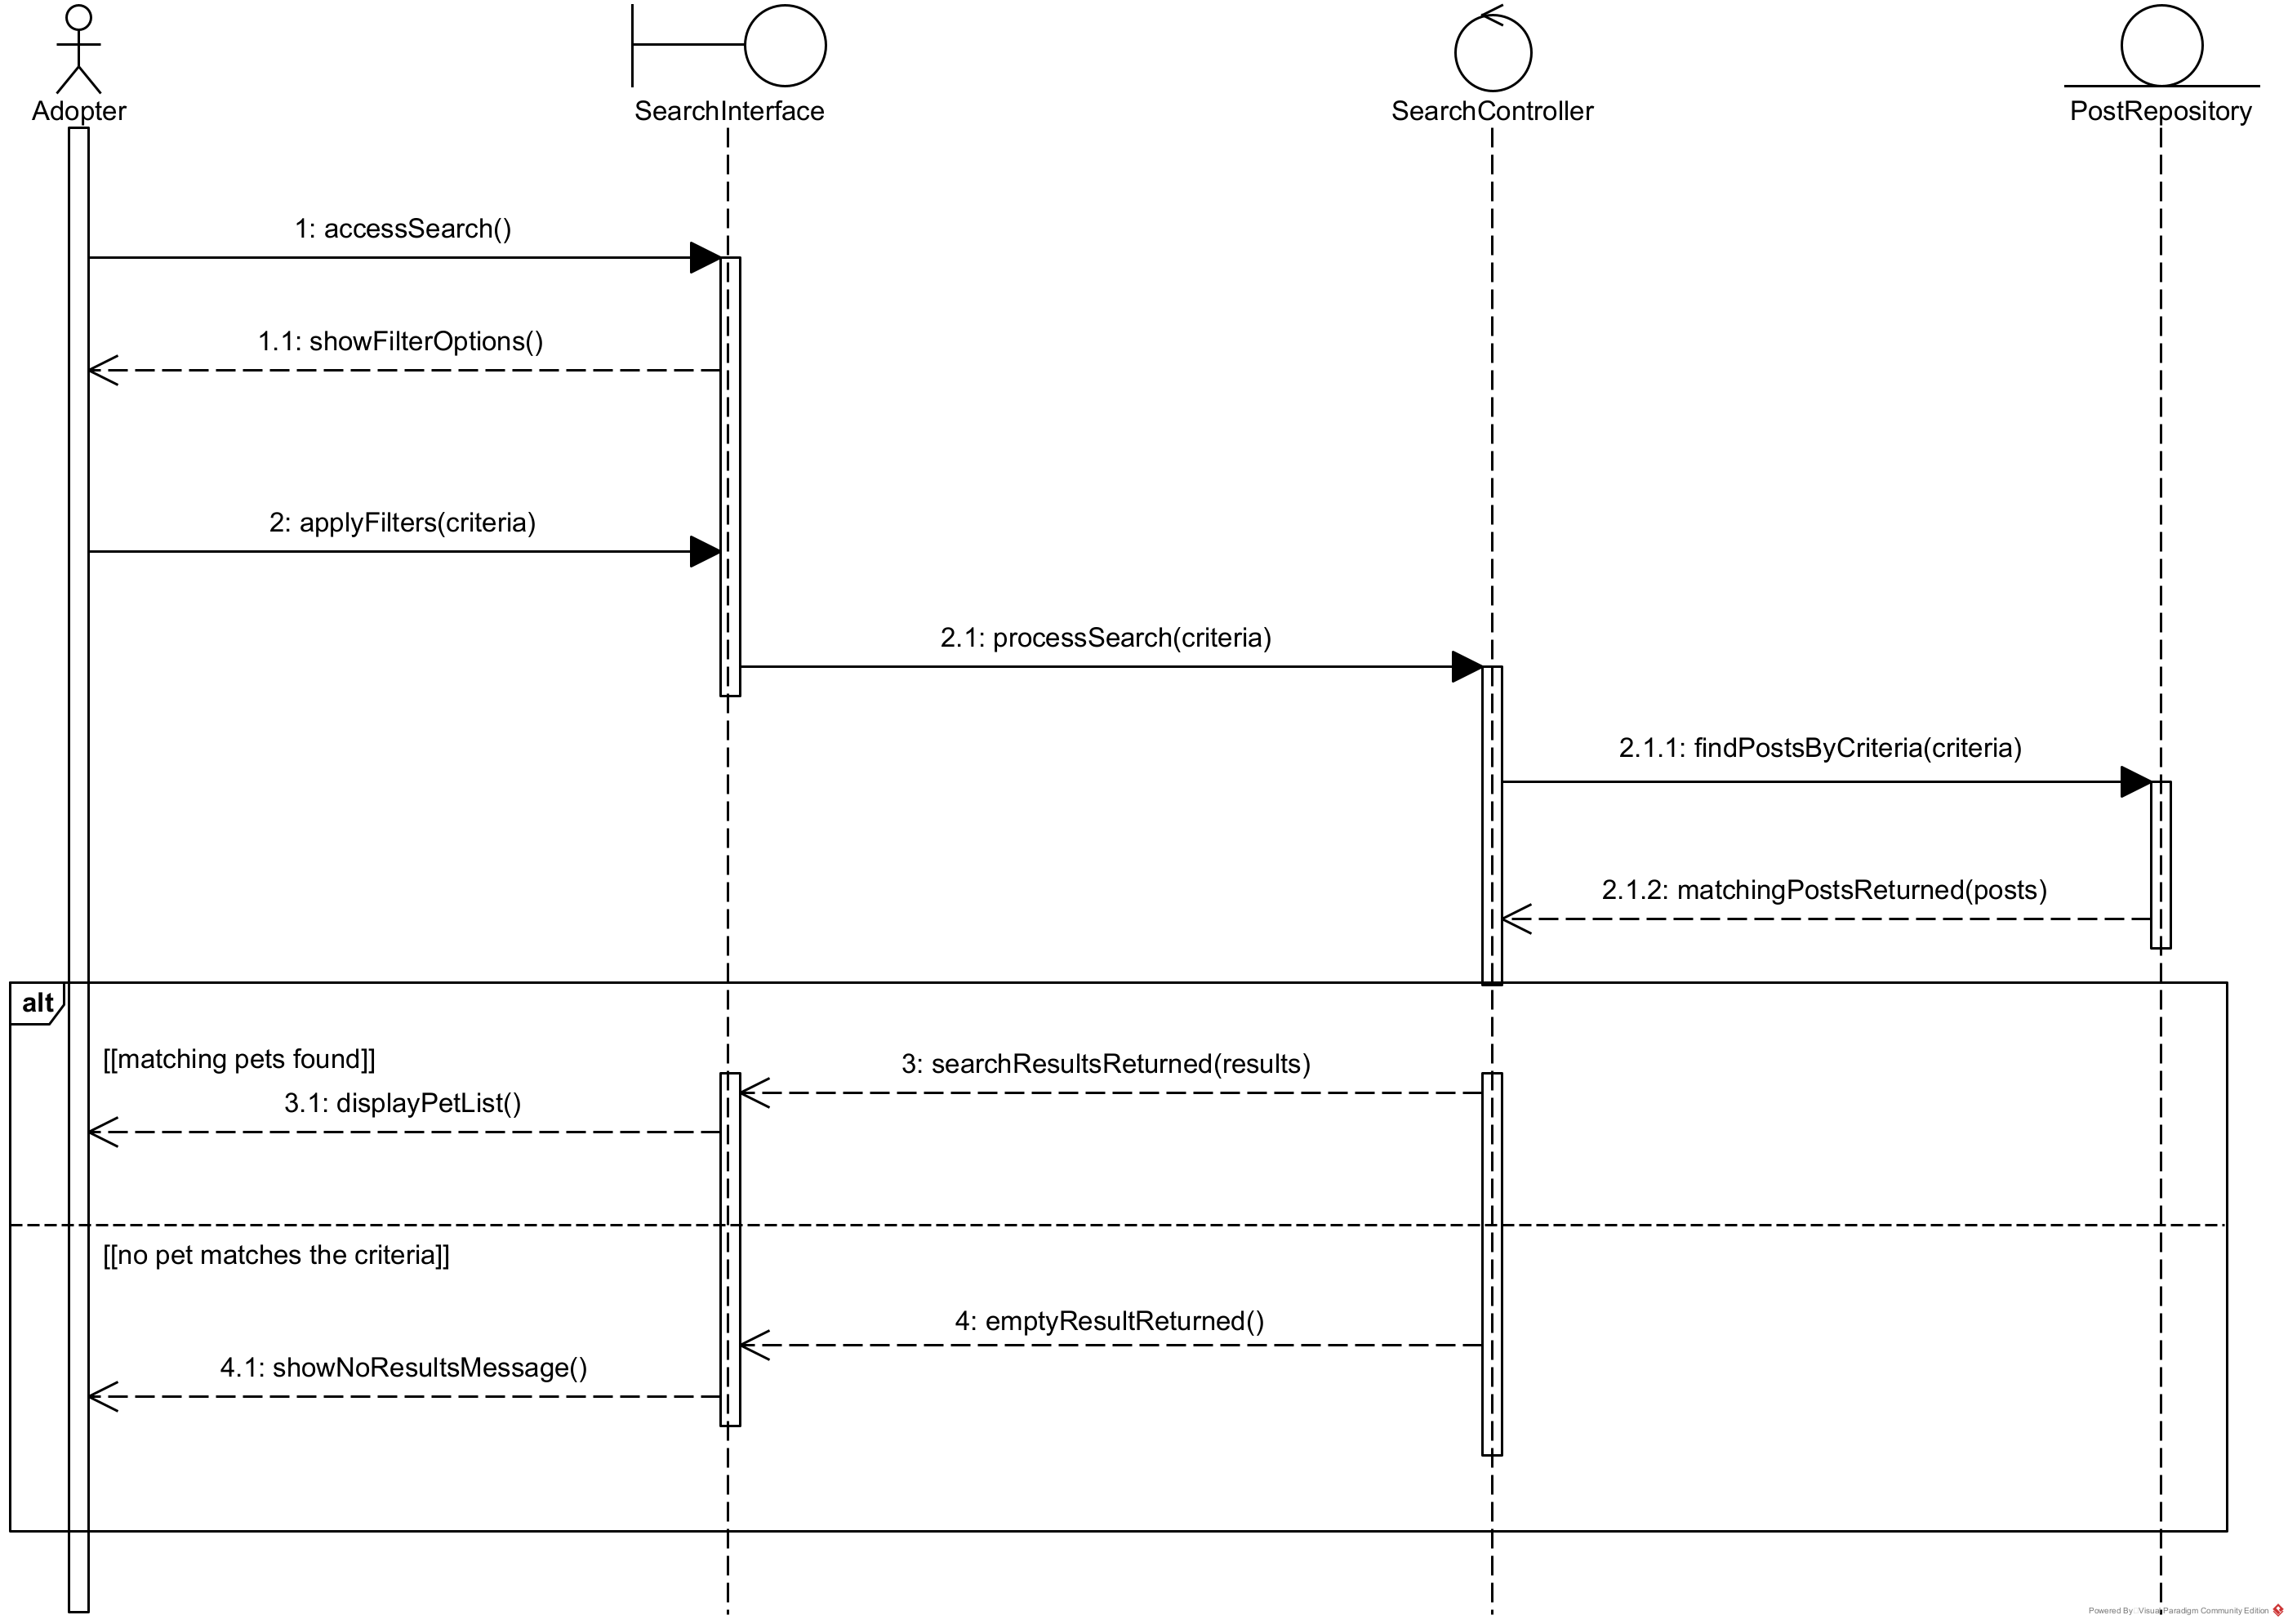
\includegraphics[width=0.72\textwidth]{figuras/DiagramaSecuencia_CU-11_MundiPets.png}
		\caption{Diagrama de secuencia del caso de uso CU-11 --- Buscar mascota disponible.}
		\label{fig:sec-cu11}
	\end{figure}
	
	\subsubsection{Configurar privacidad médica (CU-12)}
	
	Esta secuencia representa la administración de la privacidad de la
	información descrita en RF-11. El propietario selecciona, para cada
	categoría de dato sensible (ubicación, contacto y afecciones específicas),
	el nivel de visibilidad permitido. El diagrama incluye una validación
	particular: el controlador impide que el propietario restrinja
	completamente los campos médicos obligatorios para la validación
	veterinaria, devolviendo una advertencia si se intenta ocultar información
	que RD-03 exige mantener visible para las veterinarias autorizadas.
	
	\begin{figure}[H]
		\centering
		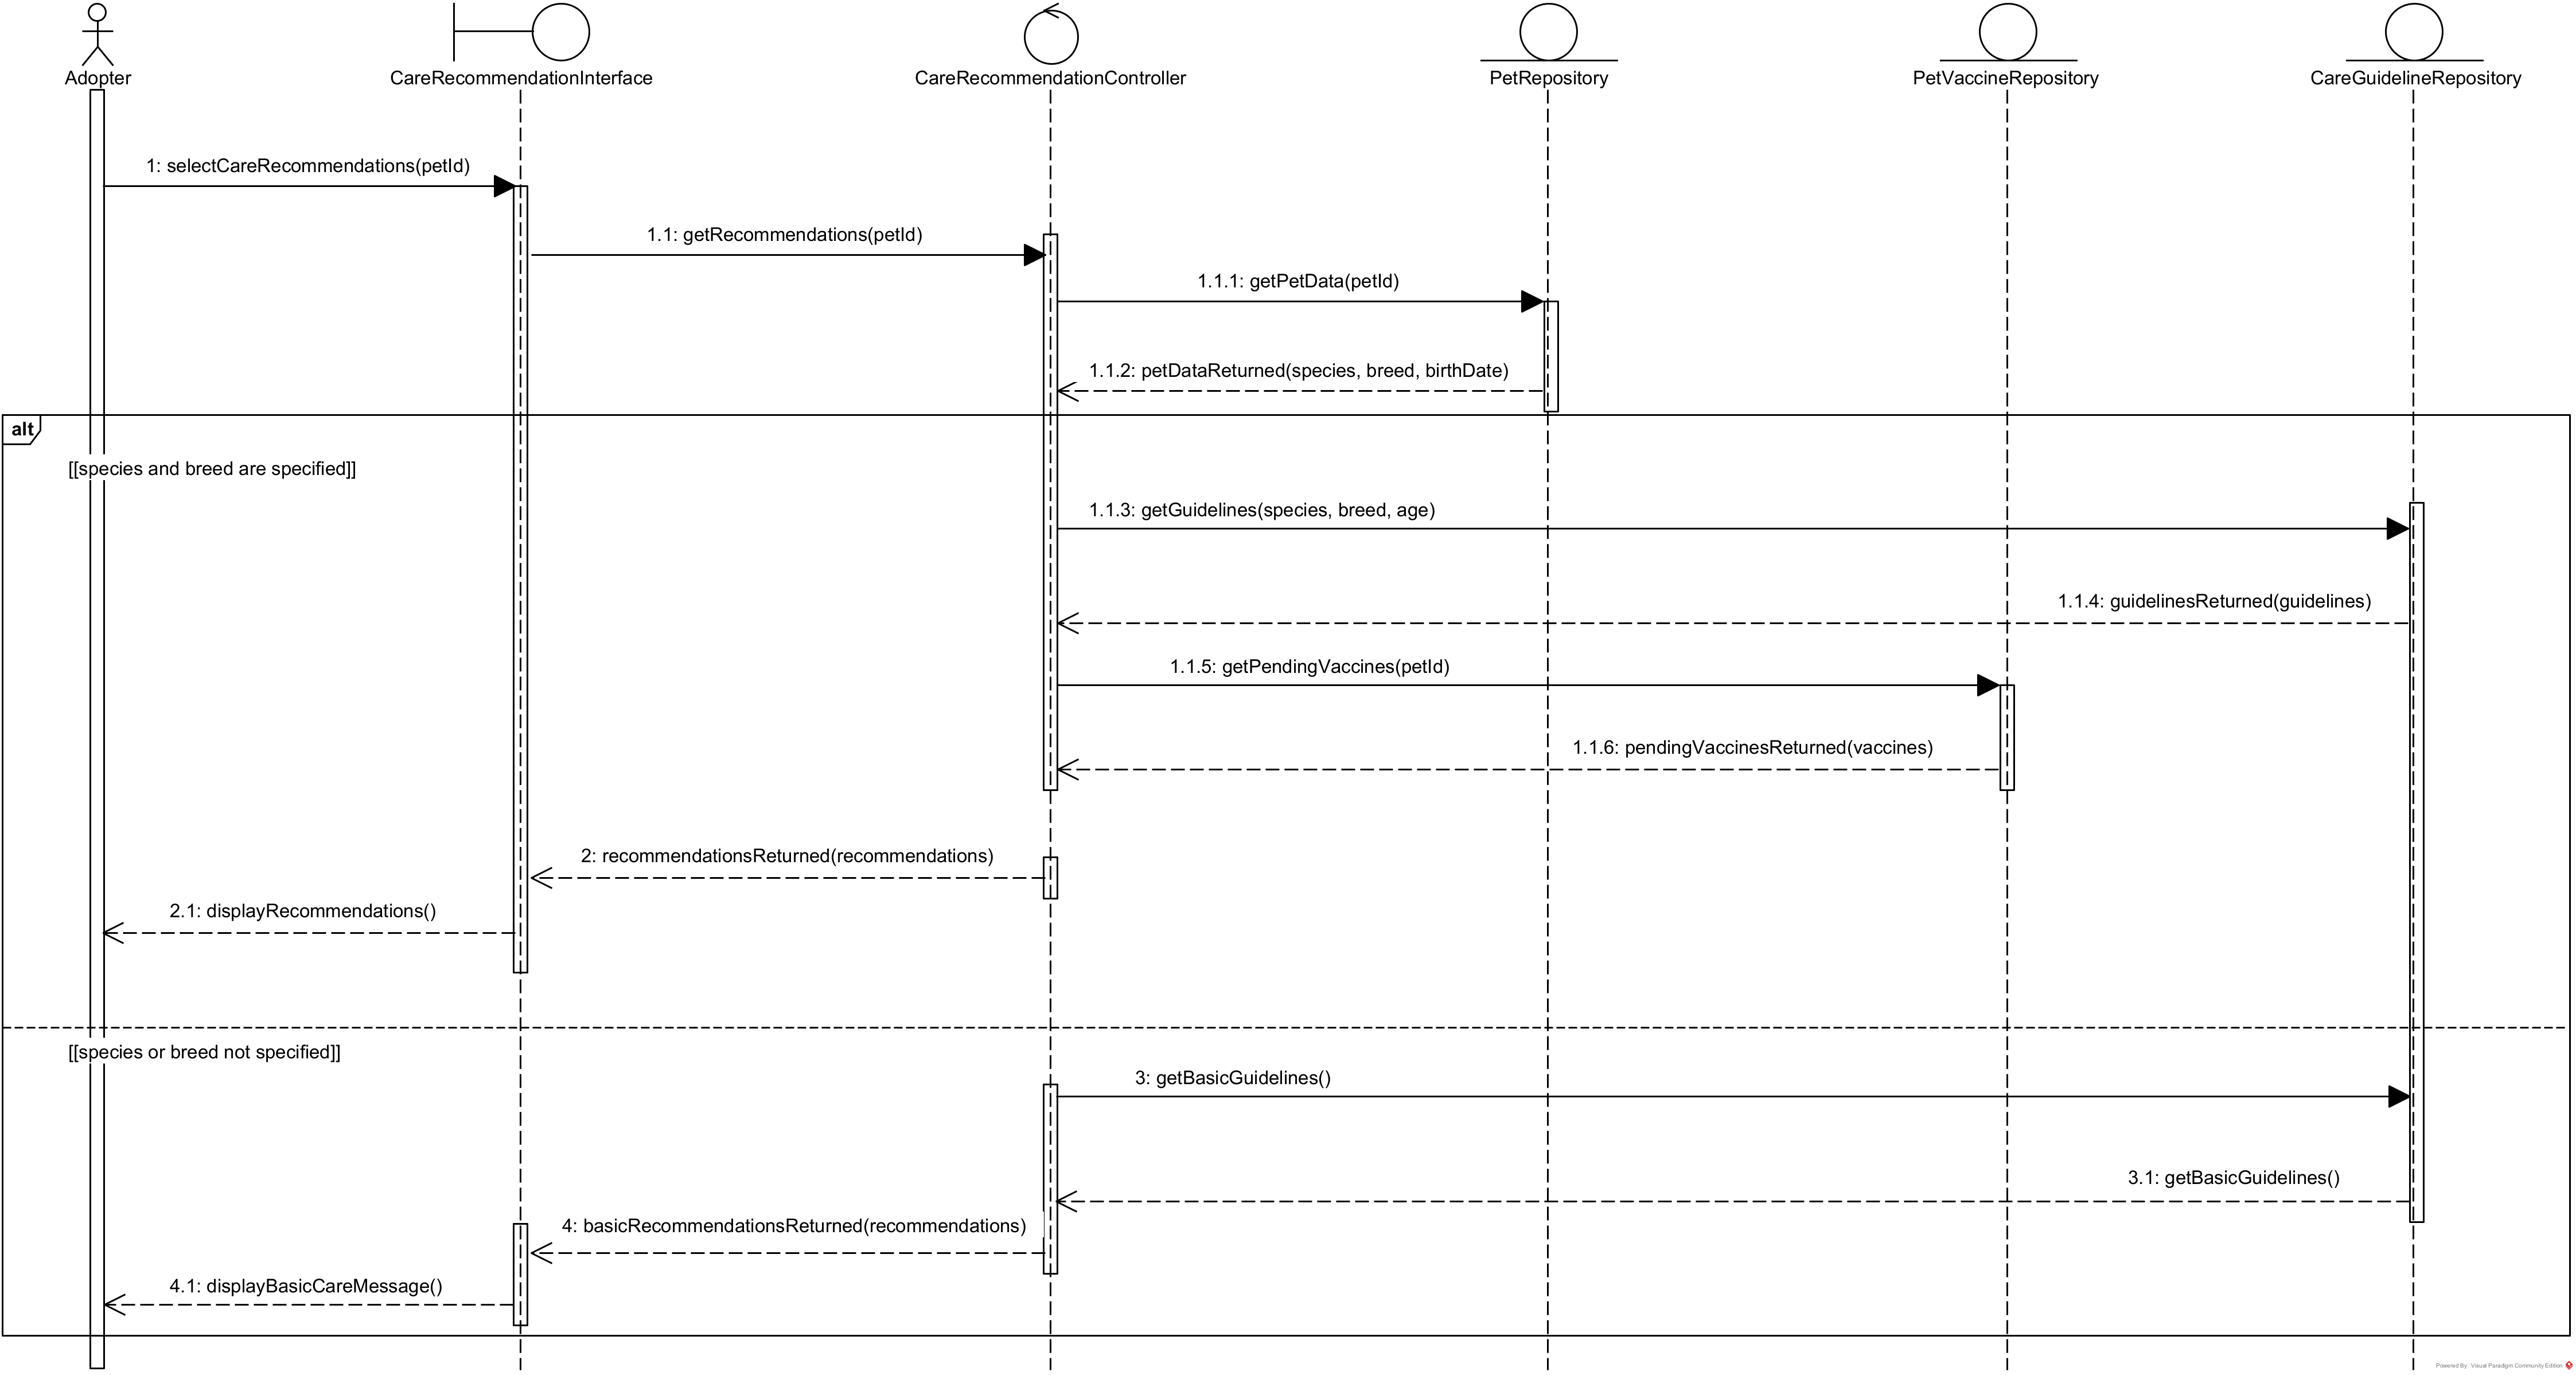
\includegraphics[width=0.72\textwidth]{figuras/DiagramaSecuencia_CU-12_MundiPets.png}
		\caption{Diagrama de secuencia del caso de uso CU-12 --- Configurar privacidad médica.}
		\label{fig:sec-cu12}
	\end{figure}
	
	\subsubsection{Evaluar compatibilidad de cruza --- verificación de parentesco (CU-13)}
	
	El diagrama de secuencia de CU-13 complementa a CU-06 al detallar
	específicamente la verificación de parentesco previa a la evaluación de
	compatibilidad (RF-06, RF-16). Antes de invocar el componente de
	inteligencia artificial, el controlador ejecuta una comprobación
	determinística sobre el grado de parentesco declarado de ambas mascotas; si
	detecta una relación incompatible, la secuencia se interrumpe y retorna
	directamente la alerta correspondiente, sin llegar a consumir el servicio de
	evaluación por IA, lo que además optimiza el uso de dicho componente ante
	casos que ya son inviables por regla de negocio.
	
	\begin{figure}[H]
		\centering
		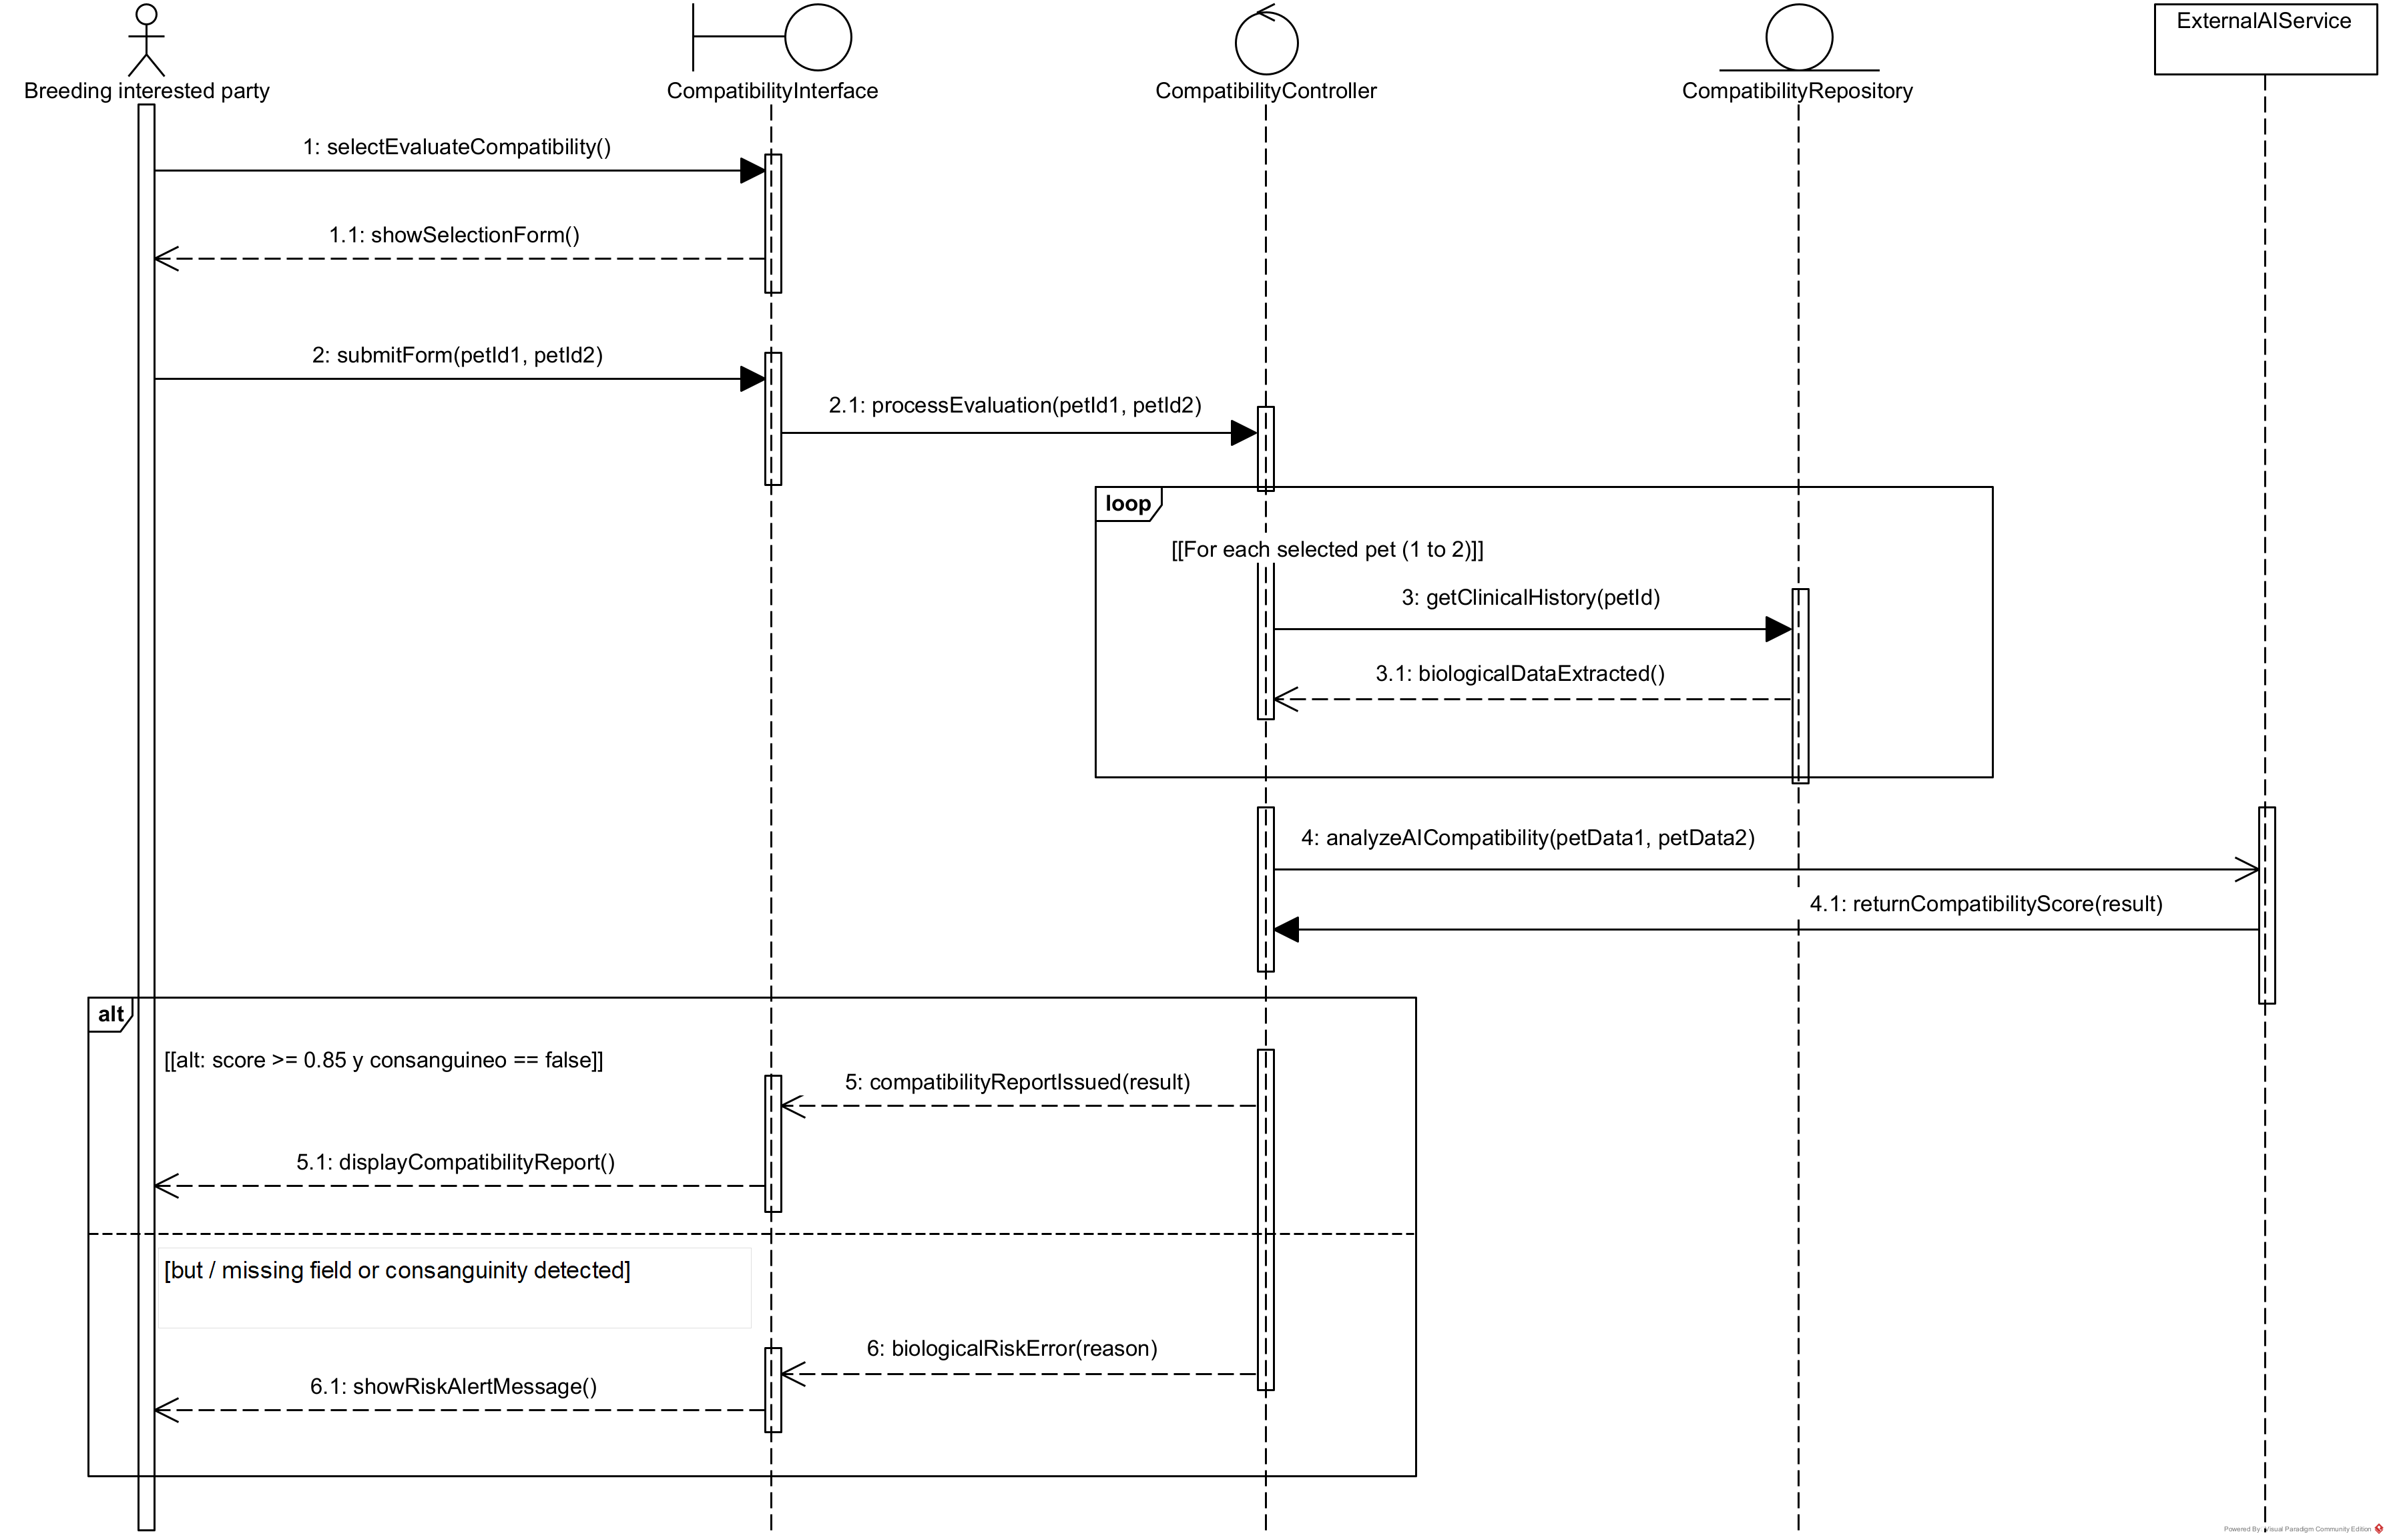
\includegraphics[width=0.72\textwidth]{figuras/DiagramaSecuencia_CU-13_MundiPets.png}
		\caption{Diagrama de secuencia del caso de uso CU-13 --- Verificación de parentesco previa a la evaluación de compatibilidad.}
		\label{fig:sec-cu13}
	\end{figure}
	
	% ------------------------------------------------------------
	\subsection{Diagramas de actividad}
	\label{sec:actividad}
	
	Los diagramas de actividad complementan a los diagramas de secuencia al
	representar el flujo de control y las decisiones lógicas dentro de cada caso
	de uso, incluyendo bifurcaciones, uniones y flujos alternos que no se
	aprecian con la misma claridad en una vista basada en intercambio de
	mensajes. A continuación se presentan los trece diagramas completos (CU-01 a
	CU-13), organizados por carriles entre el actor y el sistema.
	
	\subsubsection{Registrar mascota (CU-01)}
	
	El diagrama de actividad de CU-01 muestra el flujo completo desde que el
	propietario accede al formulario de registro hasta la confirmación del
	perfil. La rama de decisión central evalúa si los campos obligatorios
	(nombre, especie, raza, sexo, edad, estado reproductivo y al menos una
	fotografía) están completos; en caso negativo, el flujo retorna al
	formulario con el campo faltante señalado, sin avanzar hacia la validación
	de imágenes. Solo cuando la fotografía supera la validación de inteligencia
	artificial descrita en RF-17 el flujo llega al nodo final de registro
	exitoso.
	
	\begin{figure}[H]
		\centering
		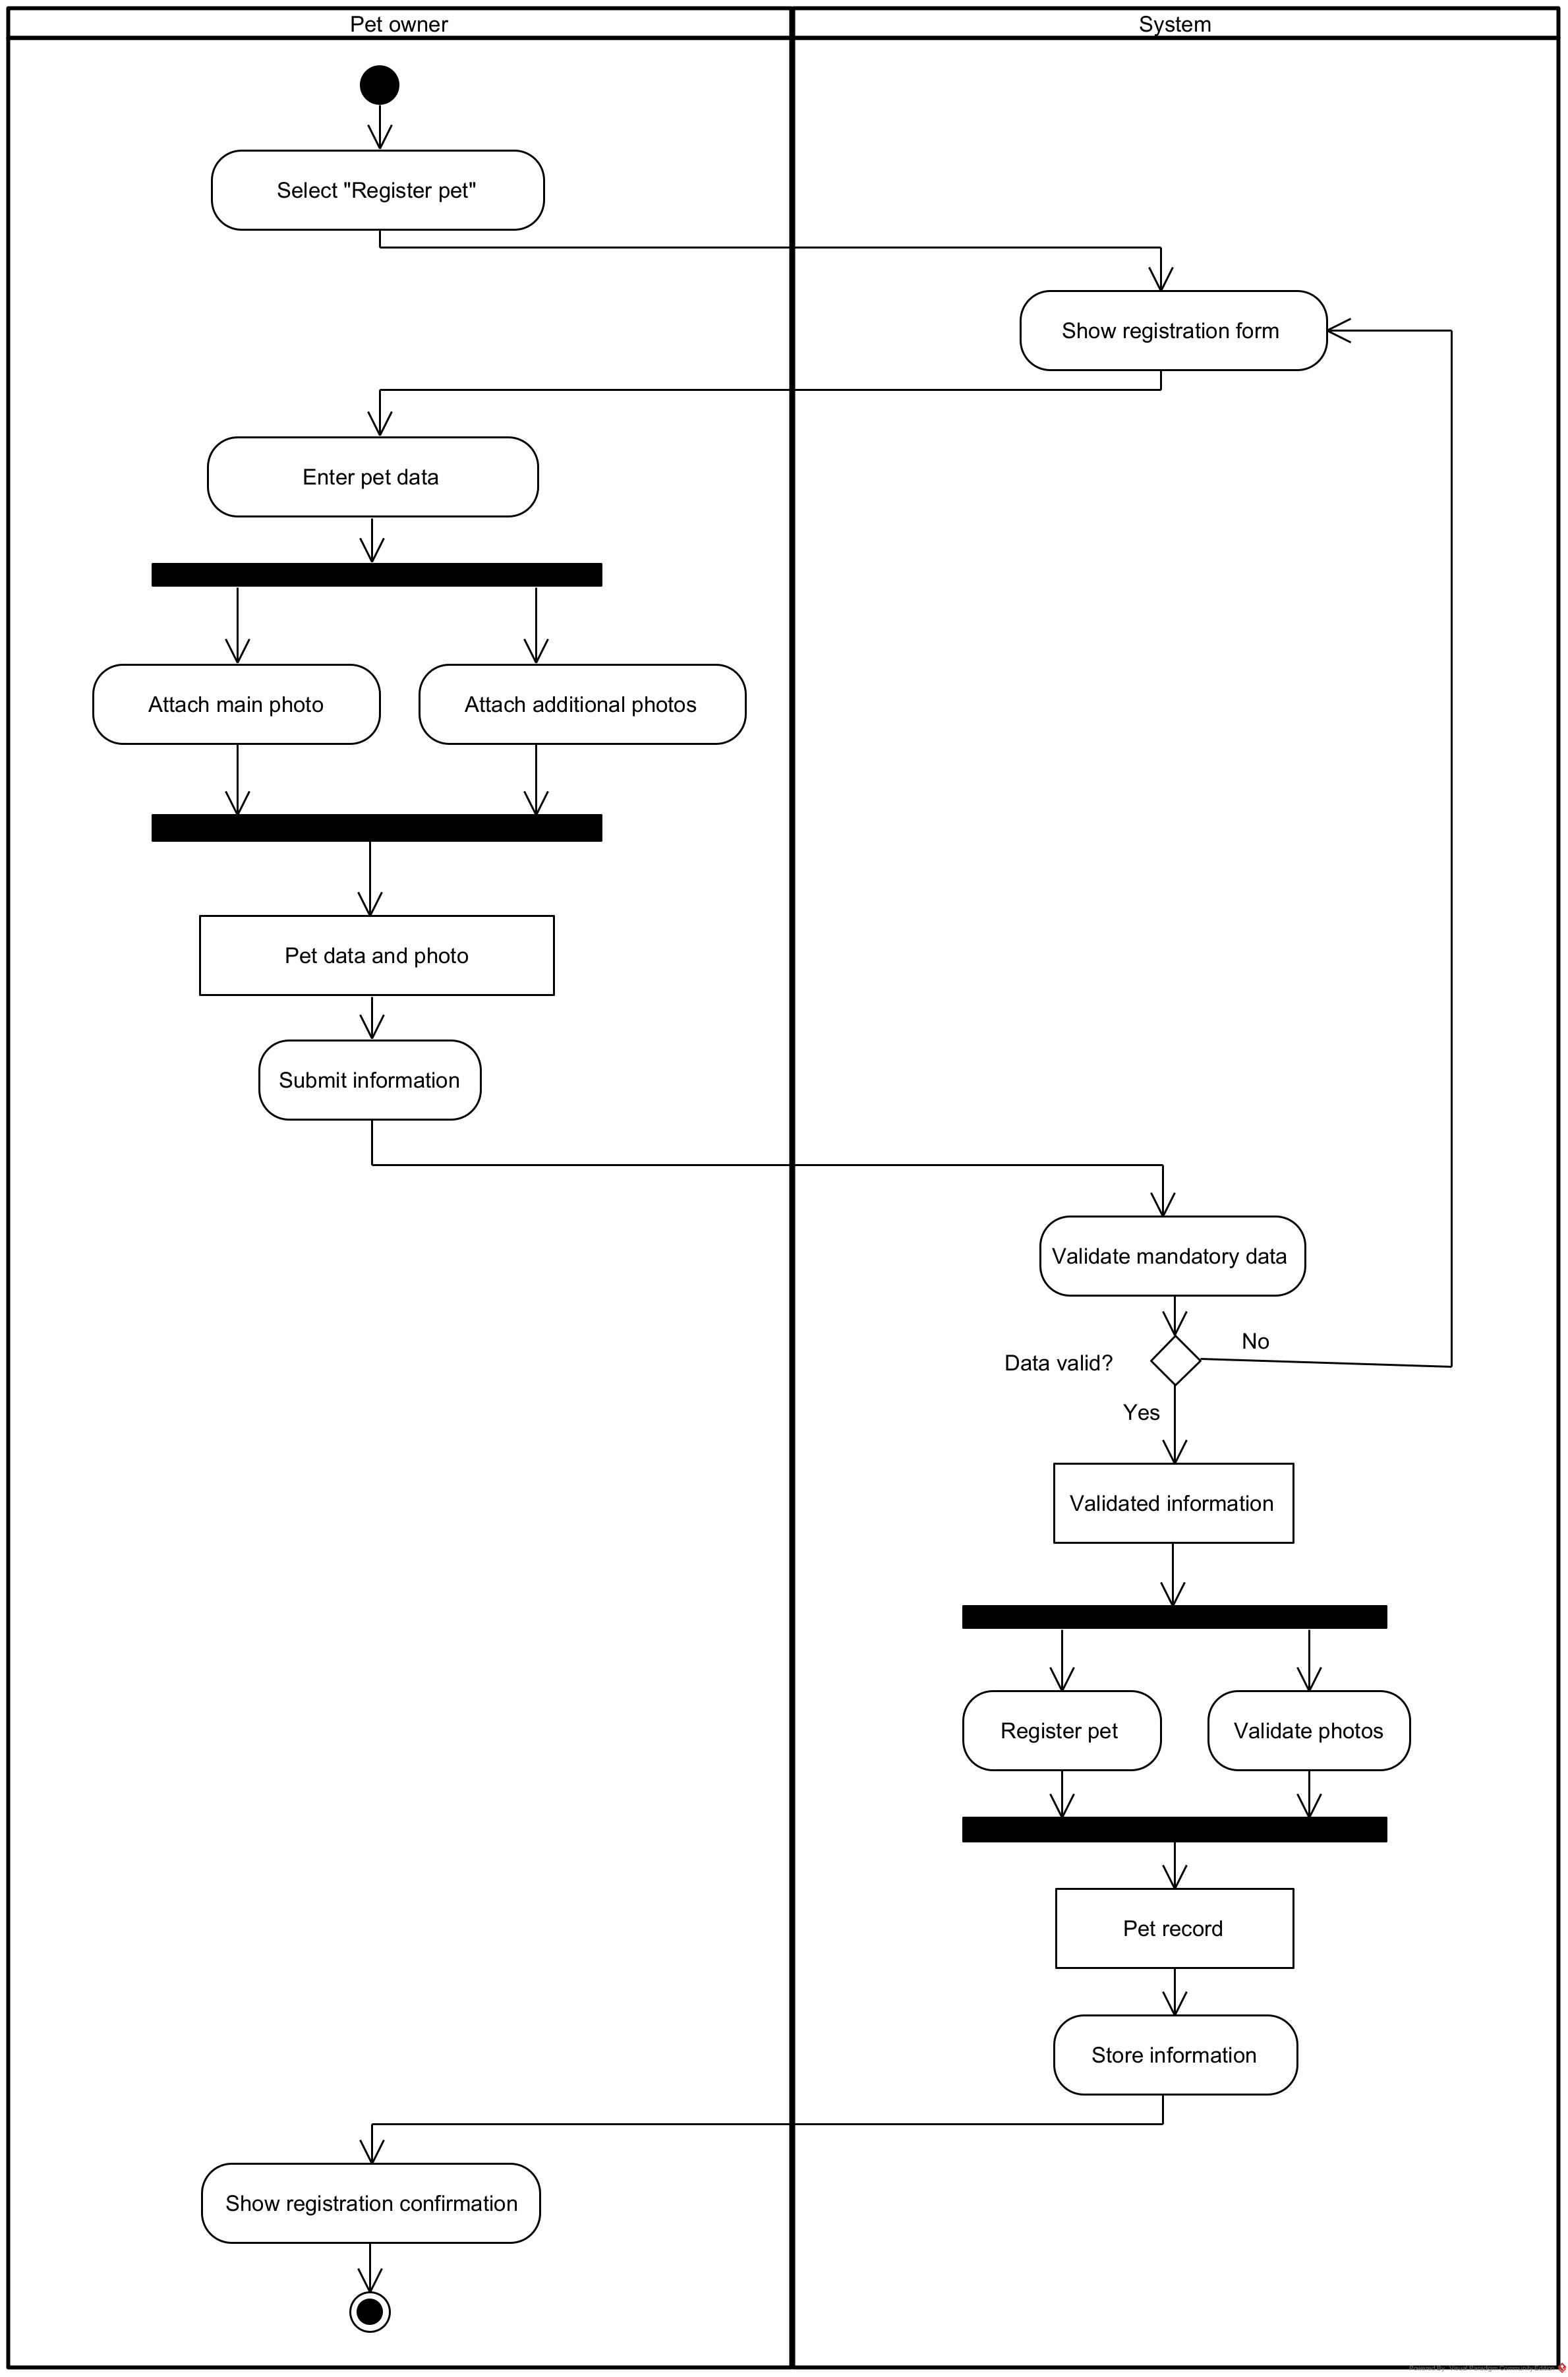
\includegraphics[width=0.66\textwidth]{figuras/DiagramaActividades_CU-01_MundiPets.png}
		\caption{Diagrama de actividad del caso de uso CU-01 --- Registrar mascota.}
		\label{fig:act-cu01}
	\end{figure}
	
	\subsubsection{Registrar historial médico y antecedentes genéticos (CU-02)}
	
	Este diagrama detalla el flujo de registro del historial médico y los
	antecedentes genéticos de una mascota (RF-02, RF-16). El carril del sistema
	bifurca el flujo según el tipo de actor que origina la actualización: cuando
	el emisor es el propietario, la actividad final marca el registro como
	pendiente de validación profesional; cuando el emisor es una veterinaria, el
	registro se marca directamente como validado, evitando un doble ciclo de
	revisión sobre información ya ingresada por un profesional autorizado.
	
	\begin{figure}[H]
		\centering
		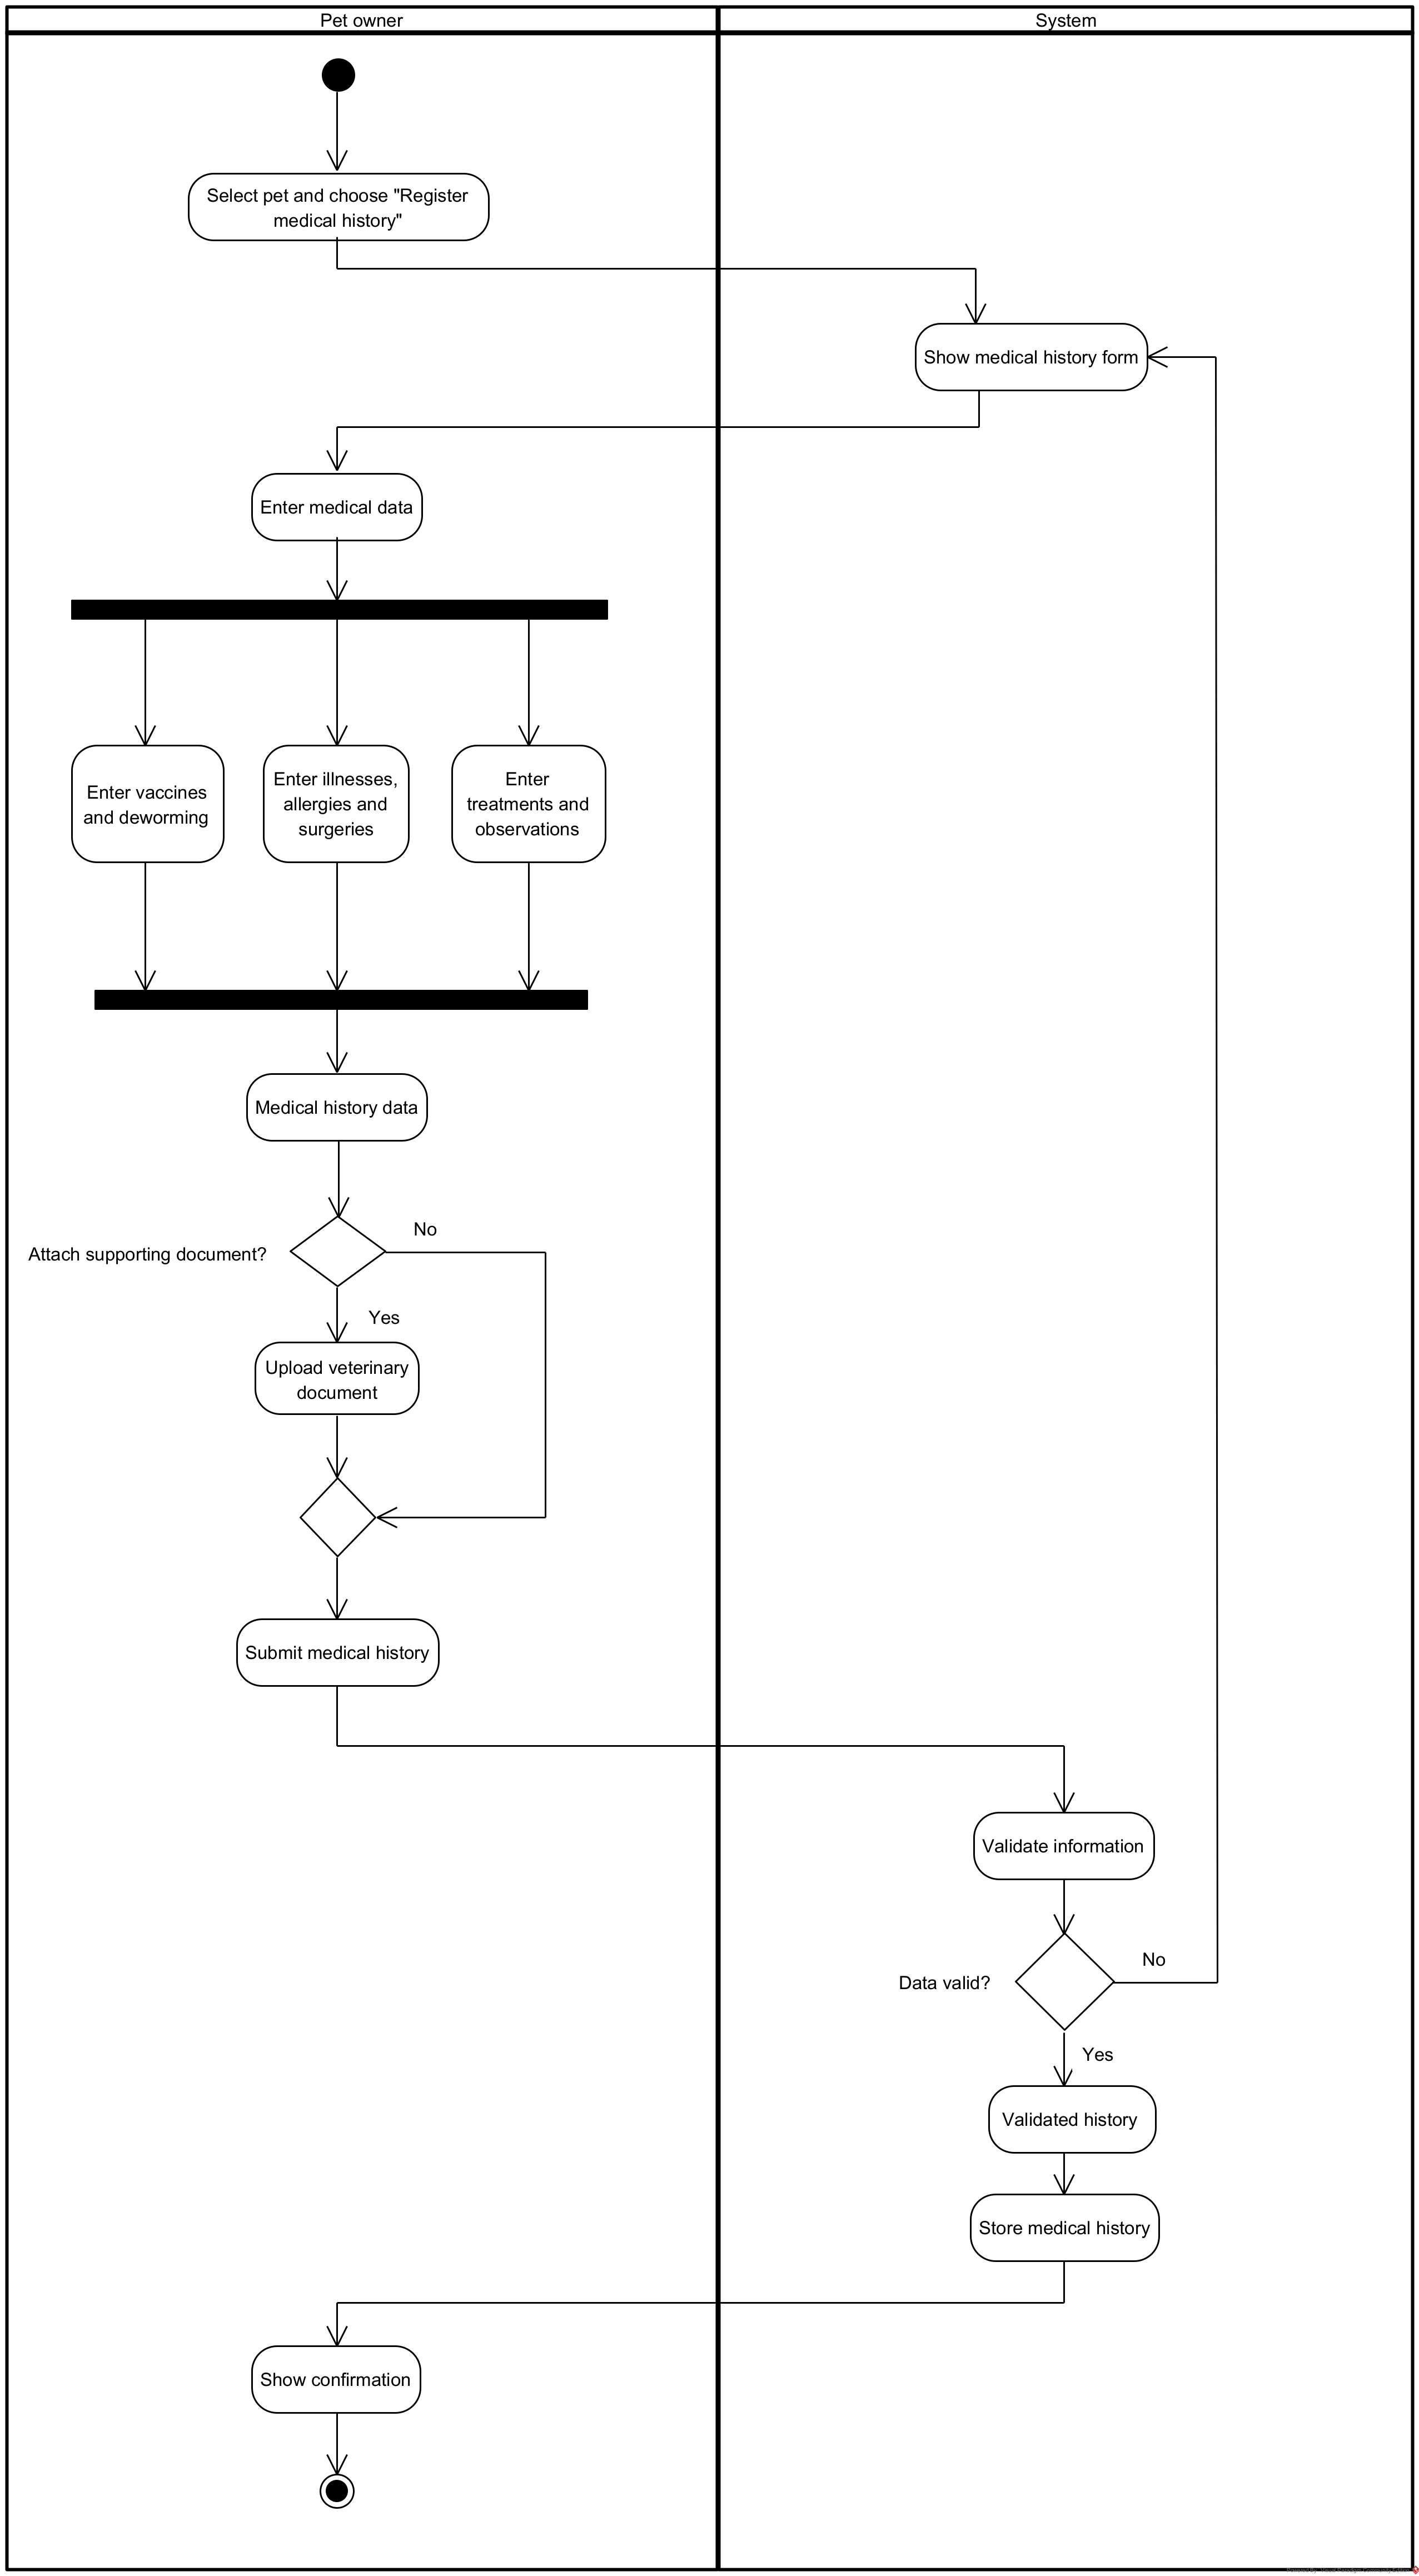
\includegraphics[width=0.56\textwidth]{figuras/DiagramaActividades_CU-02_MundiPets.png}
		\caption{Diagrama de actividad del caso de uso CU-02 --- Registrar historial médico y antecedentes genéticos.}
		\label{fig:act-cu02}
	\end{figure}
	
	\subsubsection{Cargar documento veterinario y carnet de vacunación (CU-03)}
	
	El diagrama de actividad de CU-03 representa el flujo de carga de documentos
	y actualización del carnet de vacunación (RF-14, RF-24). Tras adjuntar el
	archivo, el sistema ejecuta en paralelo la extracción de metadatos del
	documento (fecha y tipo) y su almacenamiento físico; ambas ramas se
	sincronizan en un nodo de unión antes de marcar el documento como pendiente
	de revisión, estado desde el cual queda habilitado para su posterior
	validación por parte de una veterinaria en el flujo de CU-09.
	
	\begin{figure}[H]
		\centering
		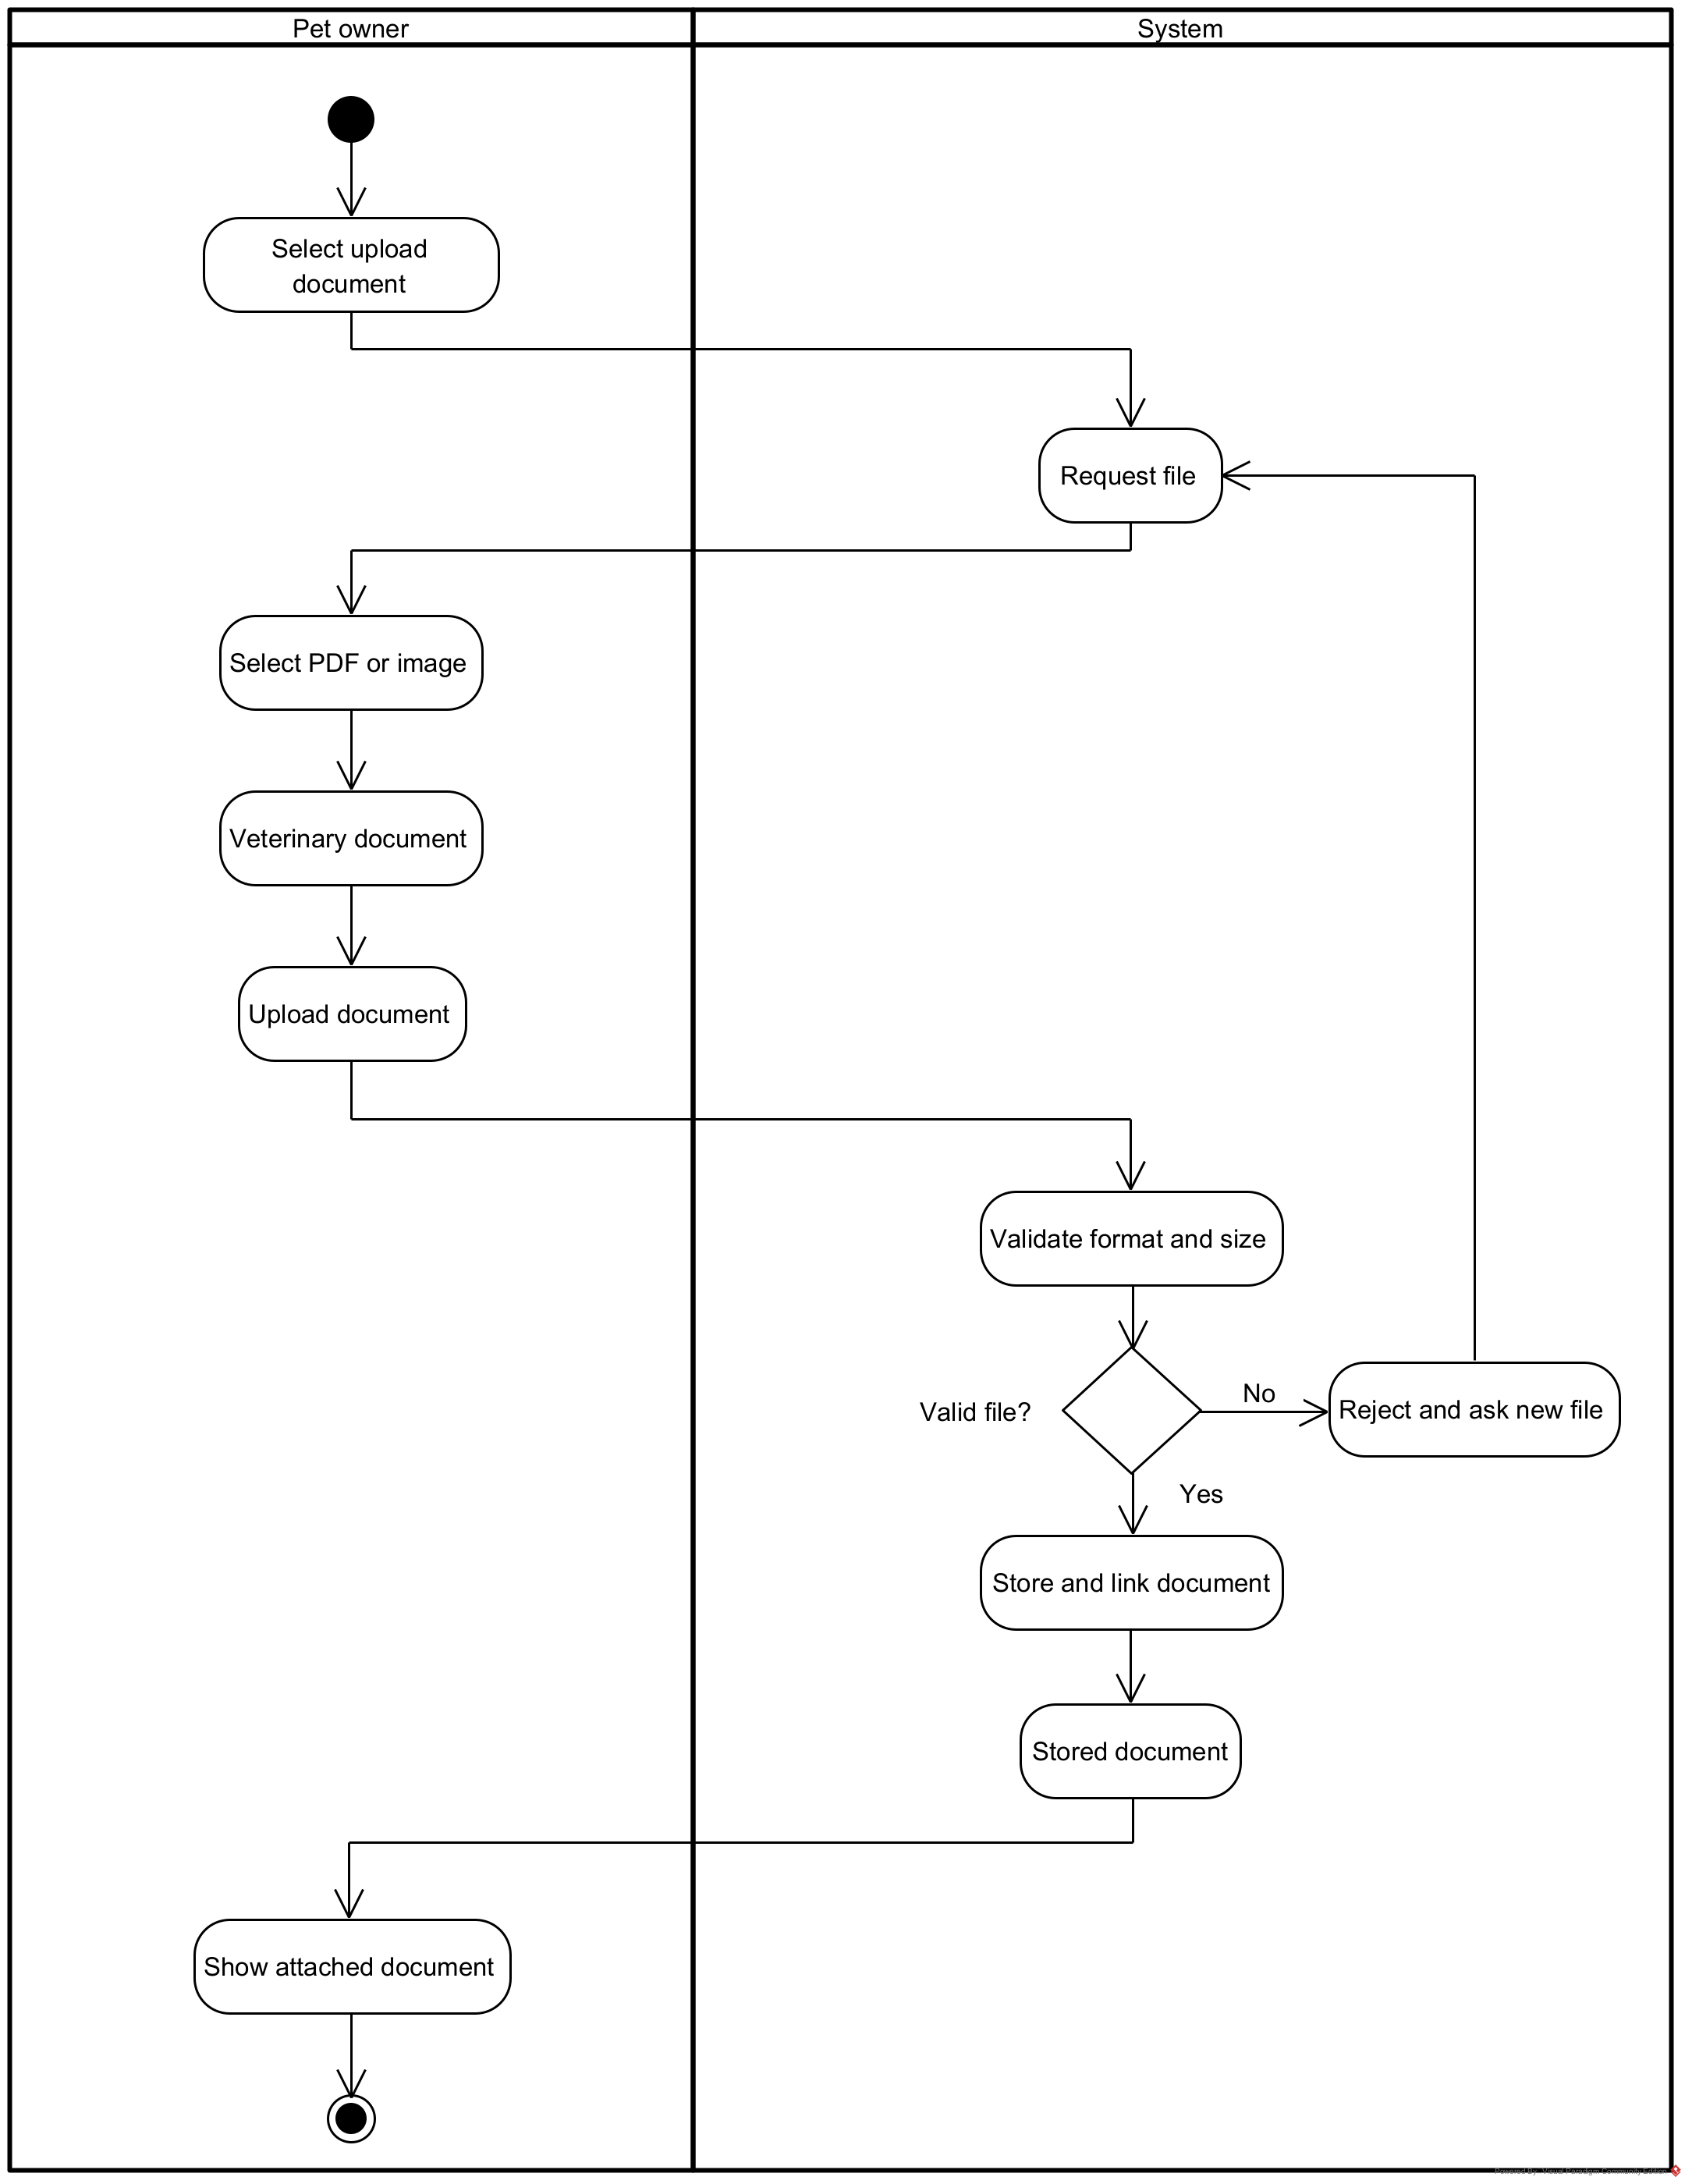
\includegraphics[width=0.77\textwidth]{figuras/DiagramaActividades_CU-03_MundiPets.png}
		\caption{Diagrama de actividad del caso de uso CU-03 --- Cargar documento veterinario y carnet de vacunación.}
		\label{fig:act-cu03}
	\end{figure}
	
	\subsubsection{Publicar mascota en adopción (CU-04)}
	
	Este diagrama expone el flujo de publicación para adopción (RF-13),
	incluyendo la bifurcación que determina si la mascota ya cuenta con una
	publicación activa. Si existe una publicación previa, el flujo ofrece al
	propietario actualizarla en lugar de crear un duplicado; si no existe, el
	sistema procede directamente a validar la completitud del perfil y a
	publicarlo en el listado de adopciones disponibles, generando la advertencia
	de perfil incompleto cuando corresponda sin bloquear la publicación.
	
	\begin{figure}[H]
		\centering
		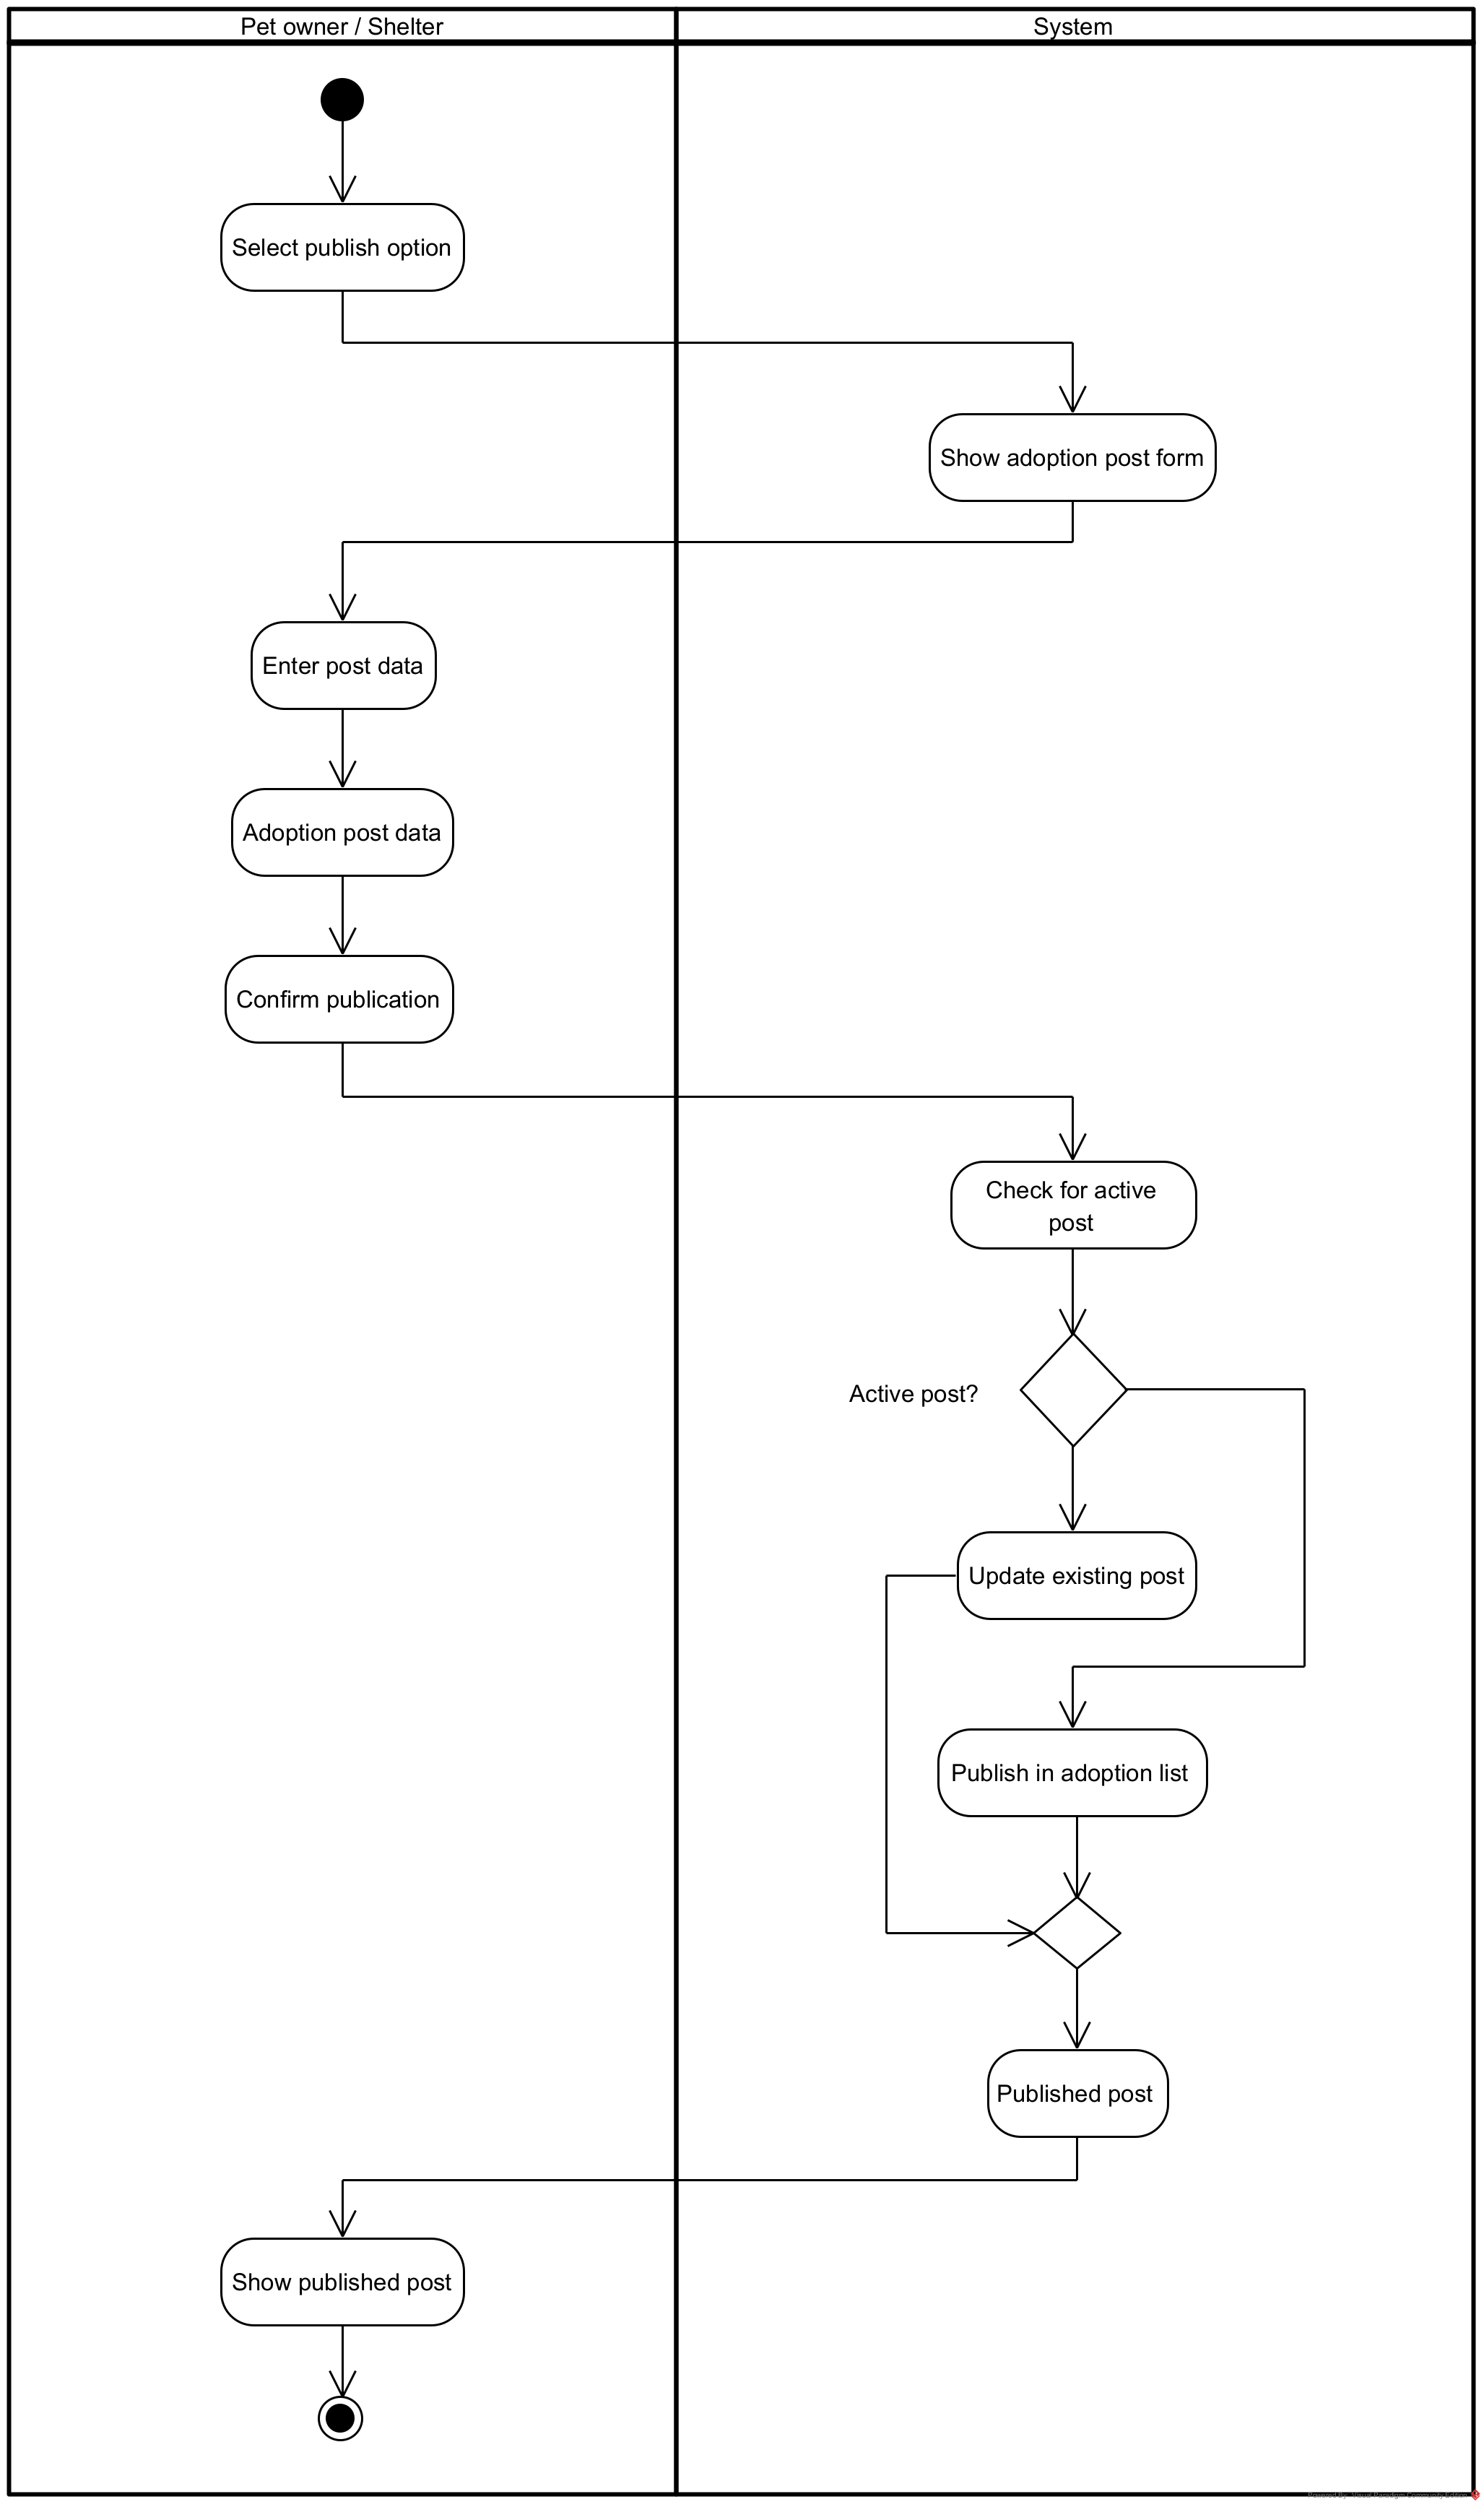
\includegraphics[width=0.60\textwidth]{figuras/DiagramaActividades_CU-04_MundiPets.png}
		\caption{Diagrama de actividad del caso de uso CU-04 --- Publicar mascota en adopción.}
		\label{fig:act-cu04}
	\end{figure}
	
	\subsubsection{Publicar mascota para cruza (CU-05)}
	
	Este diagrama representa el flujo de publicación para cruza responsable
	(RF-08, RF-13), que se diferencia del flujo de adopción por incorporar una
	verificación adicional de antecedentes genéticos y parentesco (RF-16) antes
	de habilitar la publicación. La bifurcación central del diagrama comprueba
	si la mascota cuenta con dicha información registrada; si no la tiene, el
	flujo dirige al propietario hacia el formulario de antecedentes genéticos
	antes de permitir continuar, garantizando que ninguna mascota quede
	publicada para cruza sin la información mínima que exige RF-16 para
	sustentar posteriormente la evaluación de compatibilidad.
	
	\begin{figure}[H]
		\centering
		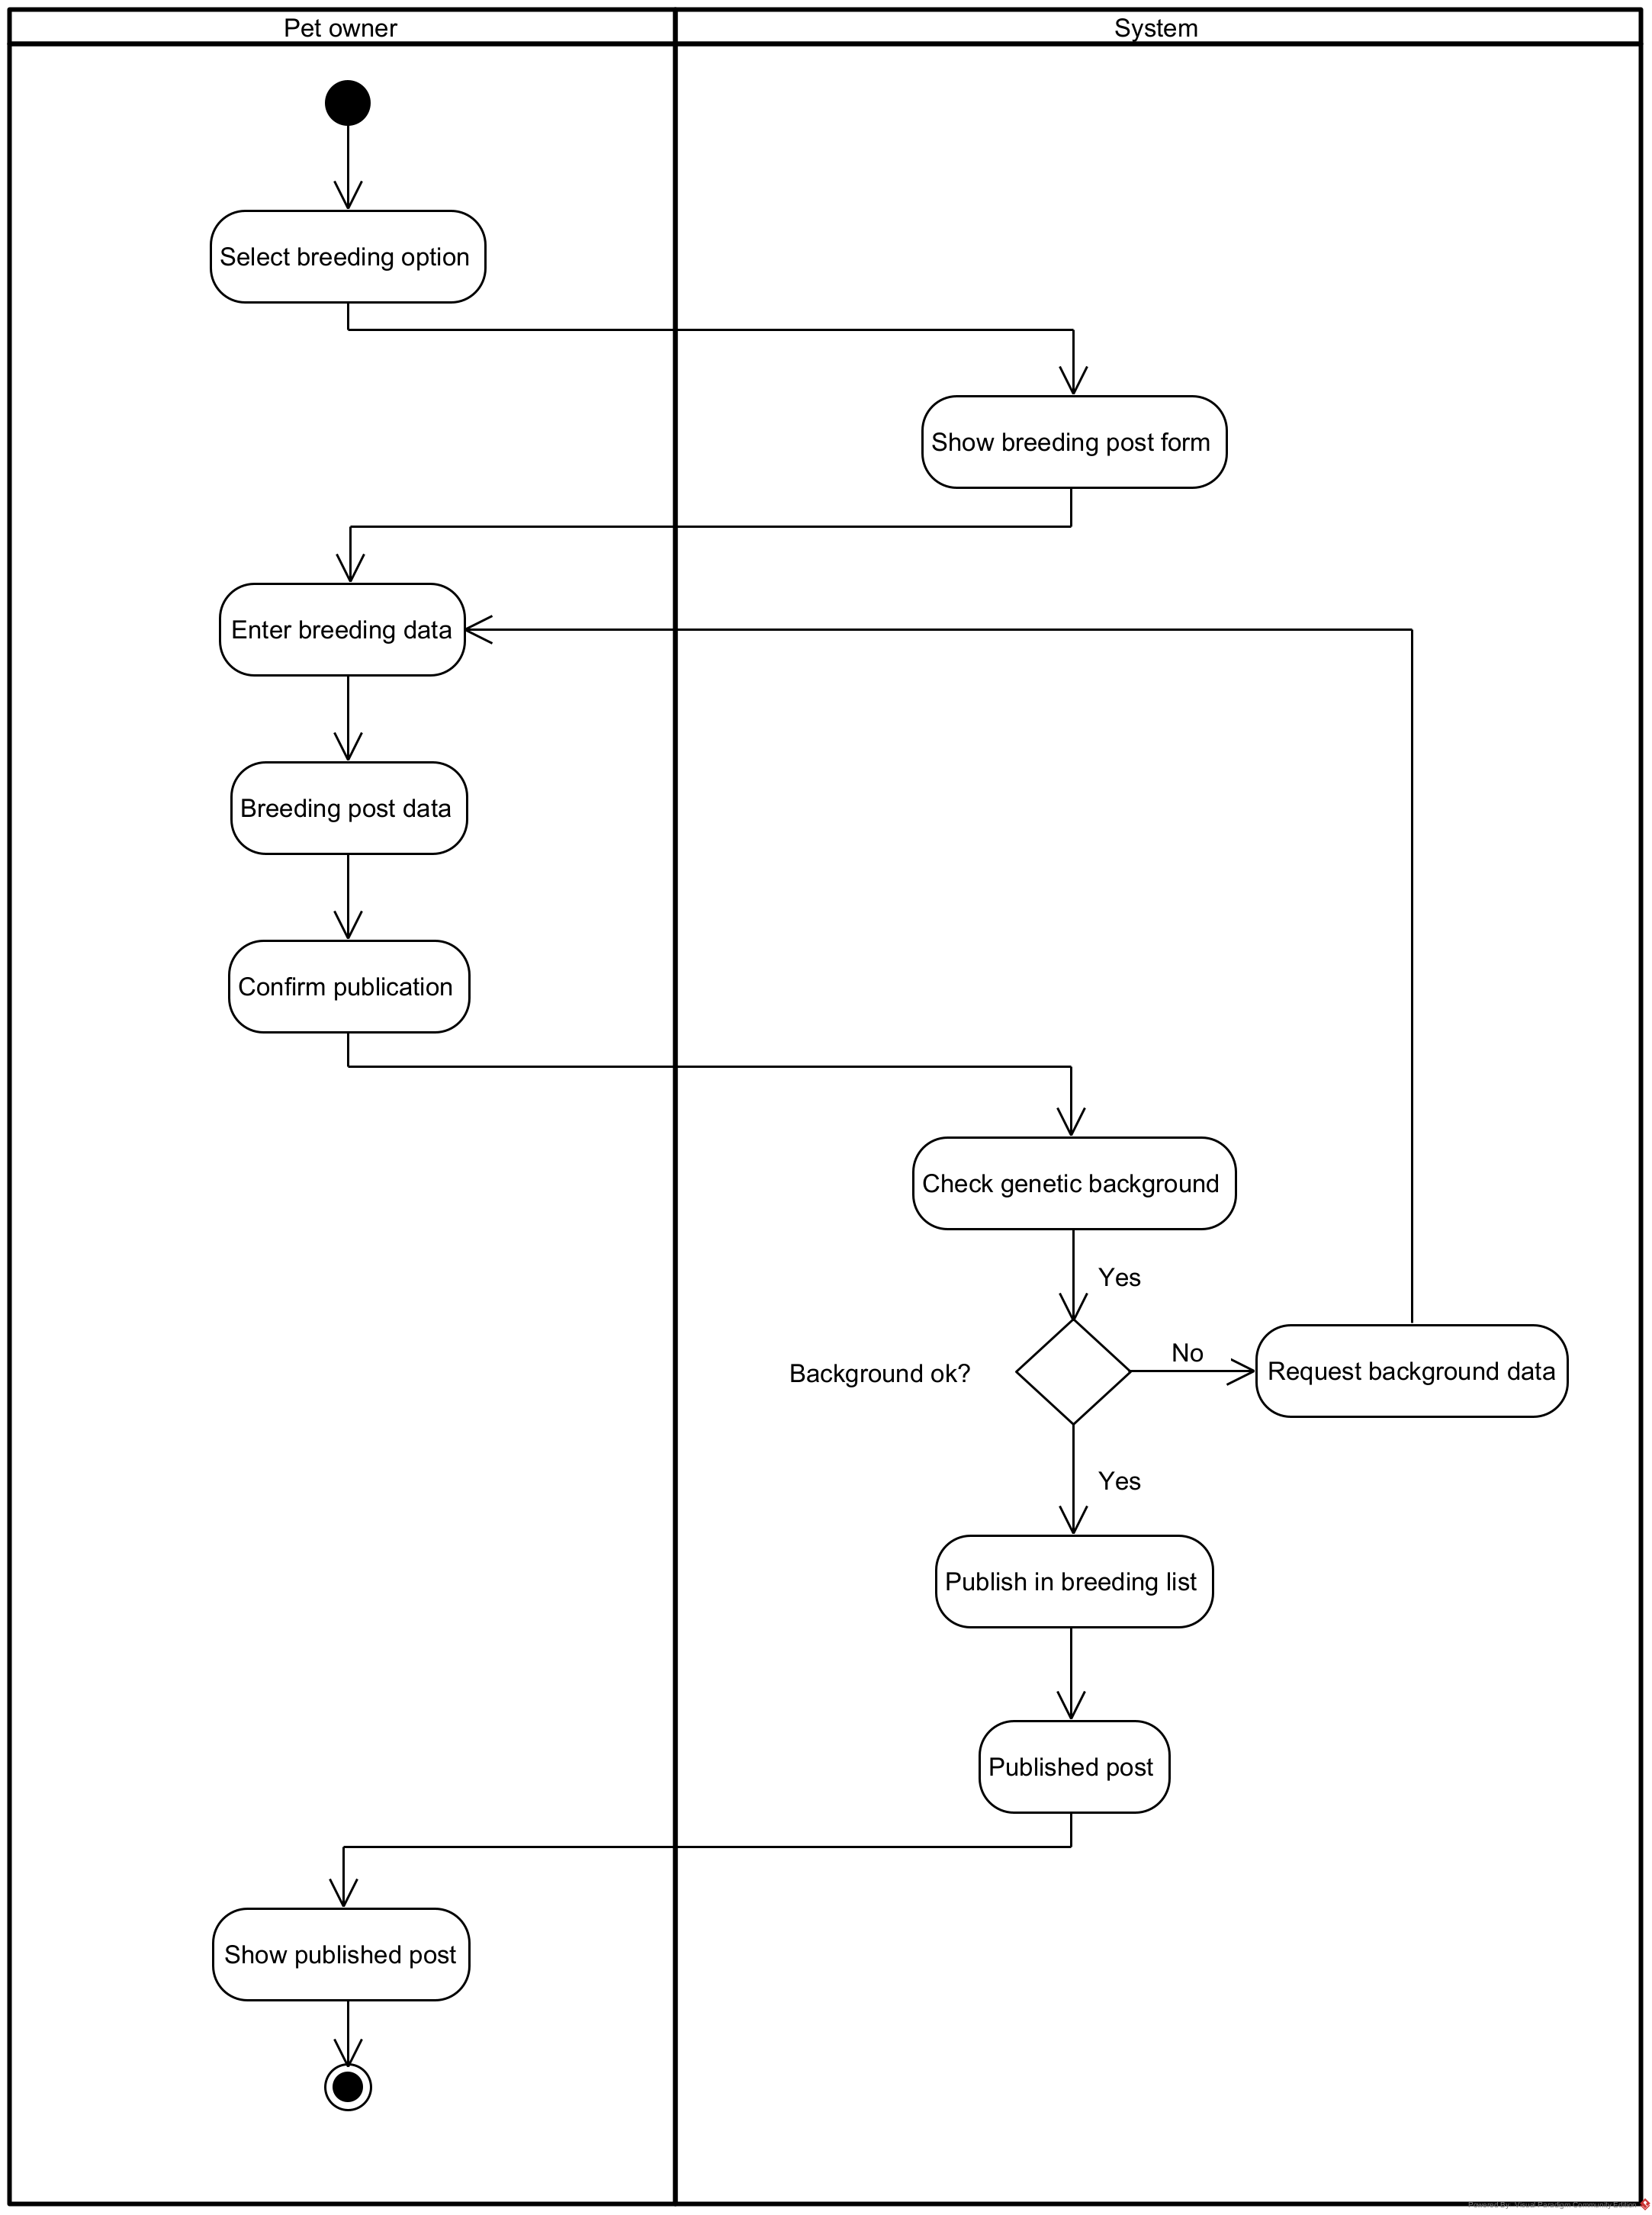
\includegraphics[width=0.75\textwidth]{figuras/DiagramaActividades_CU-05_MundiPets.png}
		\caption{Diagrama de actividad del caso de uso CU-05 --- Publicar mascota para cruza.}
		\label{fig:act-cu05}
	\end{figure}
	
	\subsubsection{Evaluar compatibilidad de cruza (CU-06)}
	
	El diagrama de actividad de CU-06 expone la lógica de decisión que subyace a
	la recomendación de compatibilidad. Tras la selección de las dos mascotas,
	el flujo se bifurca según el resultado del análisis de parentesco: si el
	sistema detecta un grado de parentesco incompatible, se activa el flujo
	alterno documentado en la especificación textual del caso de uso (flujo
	alterno 3.1 de la Tabla~\ref{tab:CU-06}), mostrando una alerta explícita
	antes de presentar cualquier resultado de compatibilidad. Solo cuando no
	existe dicha incompatibilidad el flujo principal continúa hacia la
	generación del resultado comparativo y su explicación causal asociada.
	
	\begin{figure}[H]
		\centering
		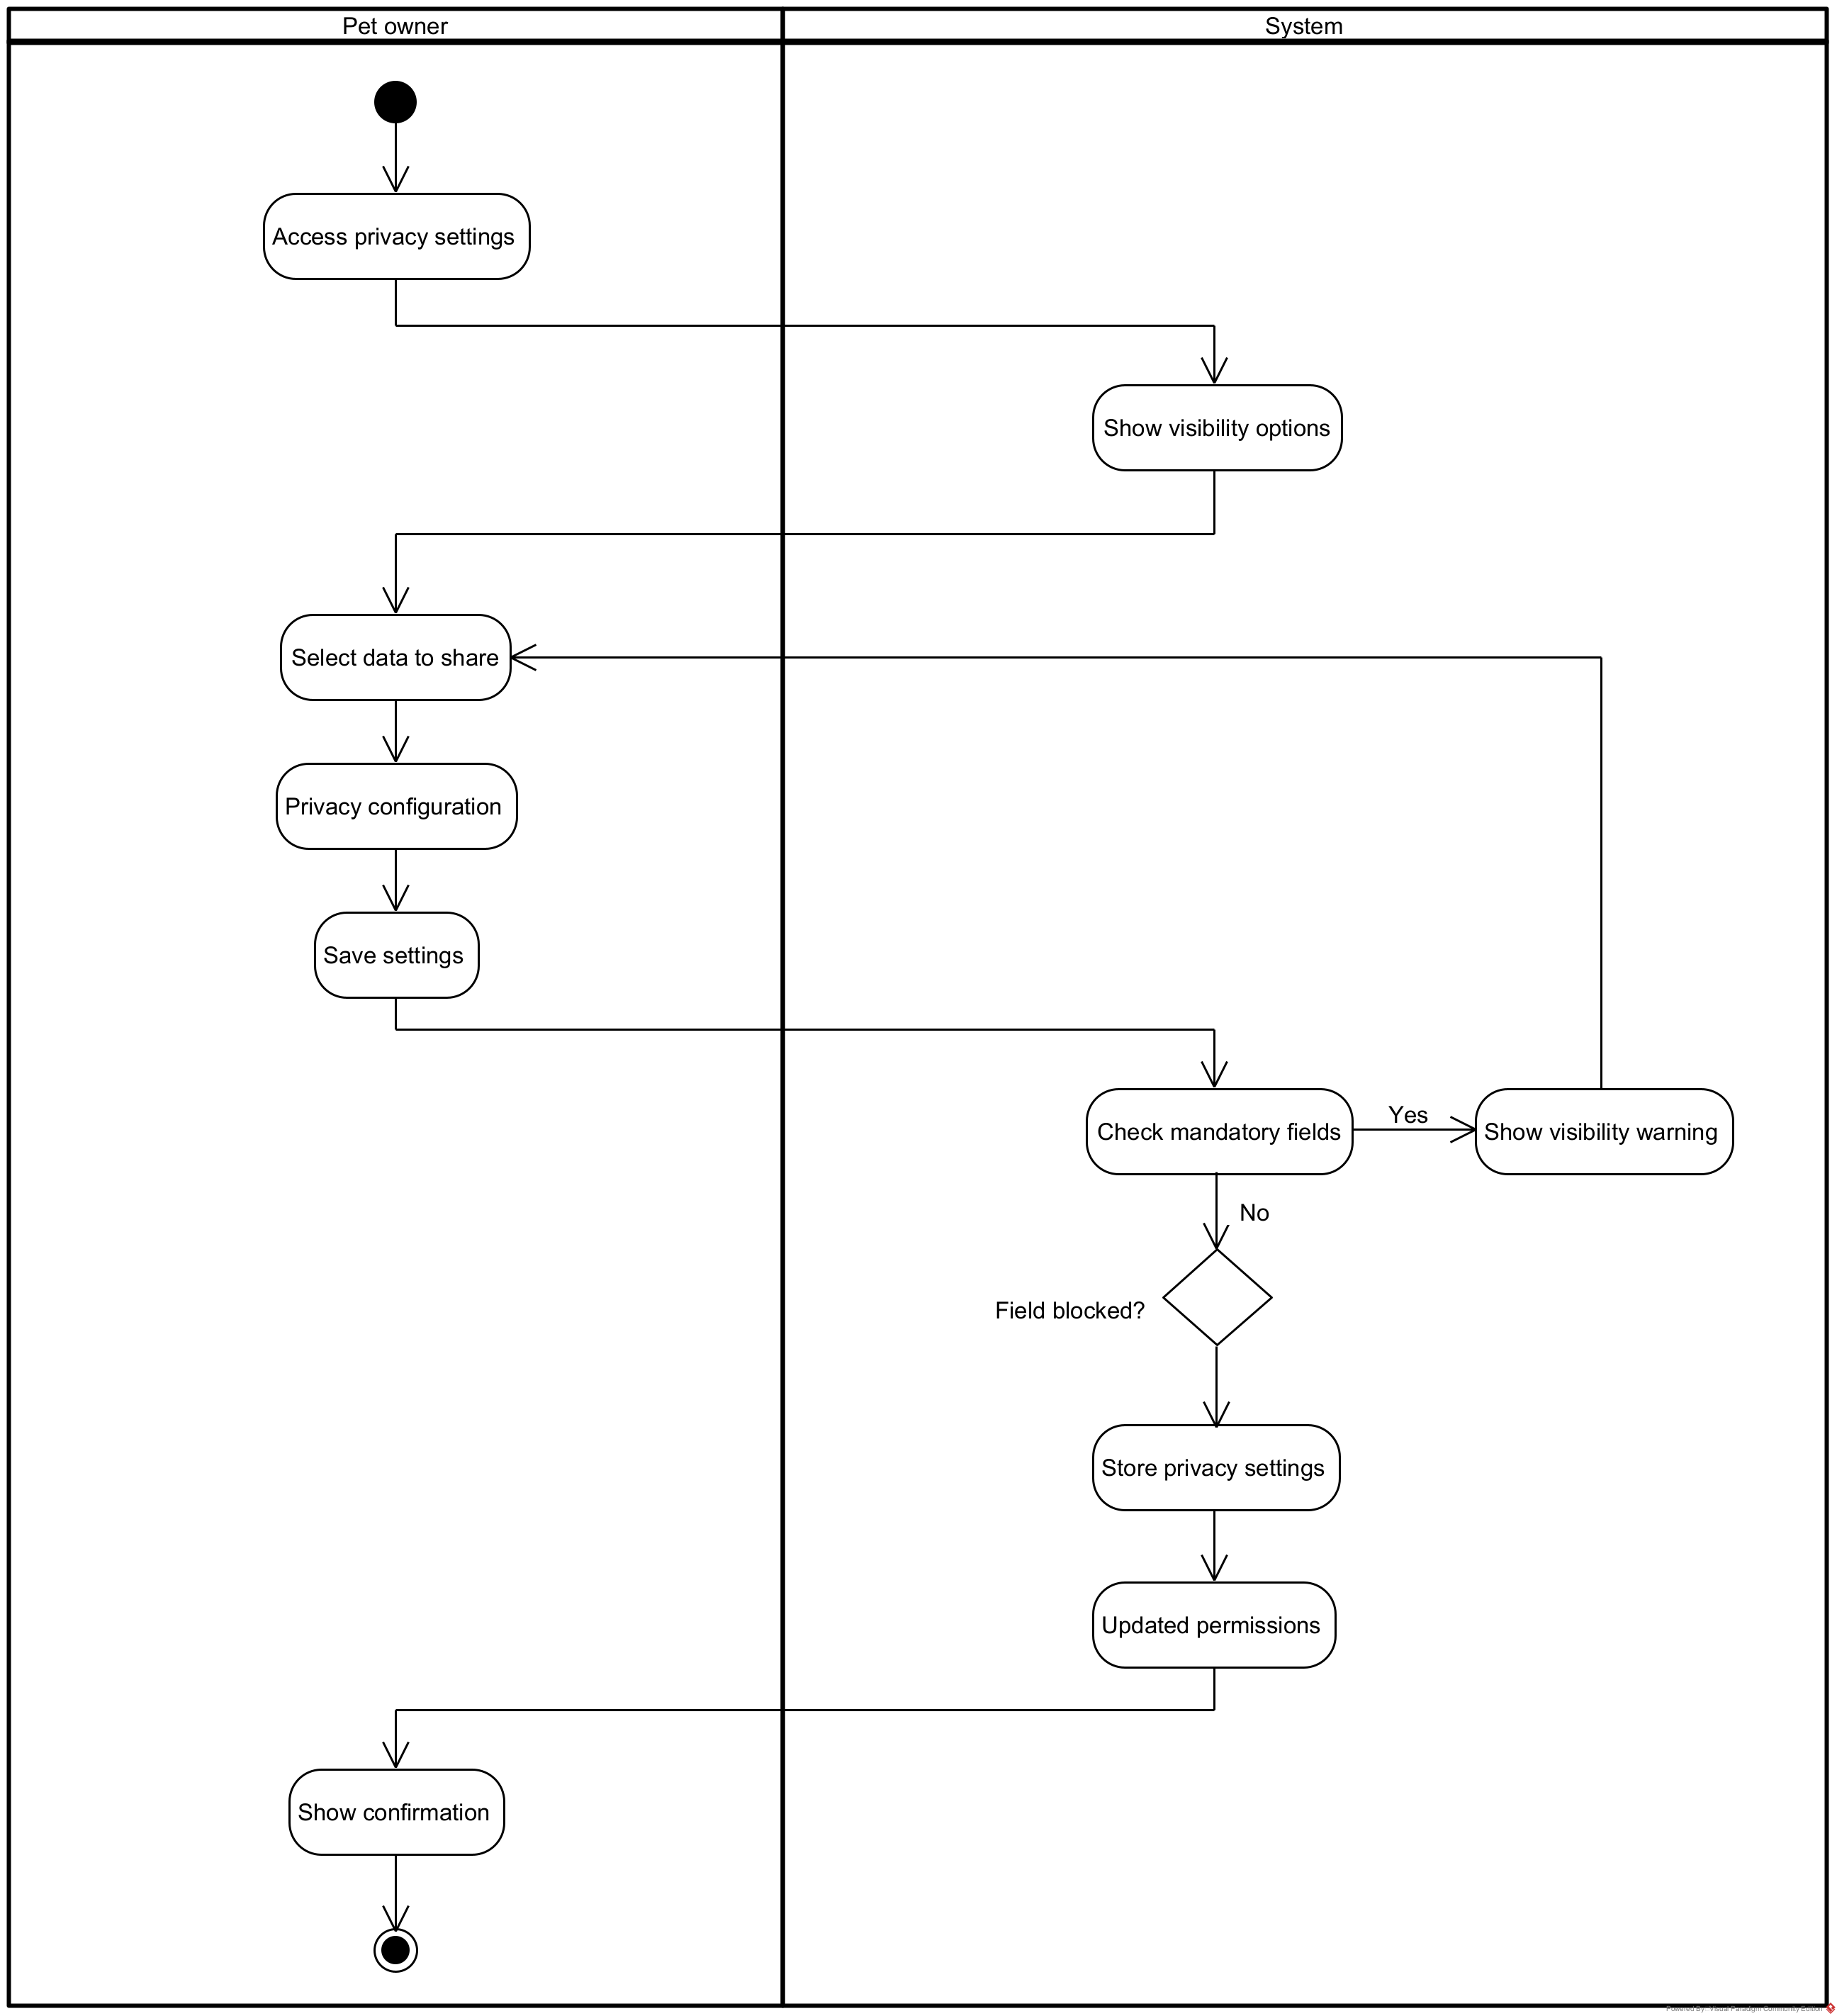
\includegraphics[width=0.90\textwidth]{figuras/DiagramaActividades_CU-06_MundiPets.png}
		\caption{Diagrama de actividad del caso de uso CU-06 --- Evaluar compatibilidad de cruza.}
		\label{fig:act-cu06}
	\end{figure}
	
	\subsubsection{Consultar historial de procesos de adopción y cruza (CU-07)}
	
	Este diagrama modela el flujo de consulta del historial de procesos (RF-15).
	Tras la solicitud del propietario, el sistema recupera en paralelo las
	solicitudes de adopción y de cruza registradas para sus mascotas, las
	combina en una sola vista ordenada por fecha y verifica, para cada una, el
	nivel de información que puede mostrarse según el estado del proceso, antes
	de presentar la línea de tiempo consolidada al propietario.
	
	\begin{figure}[H]
		\centering
		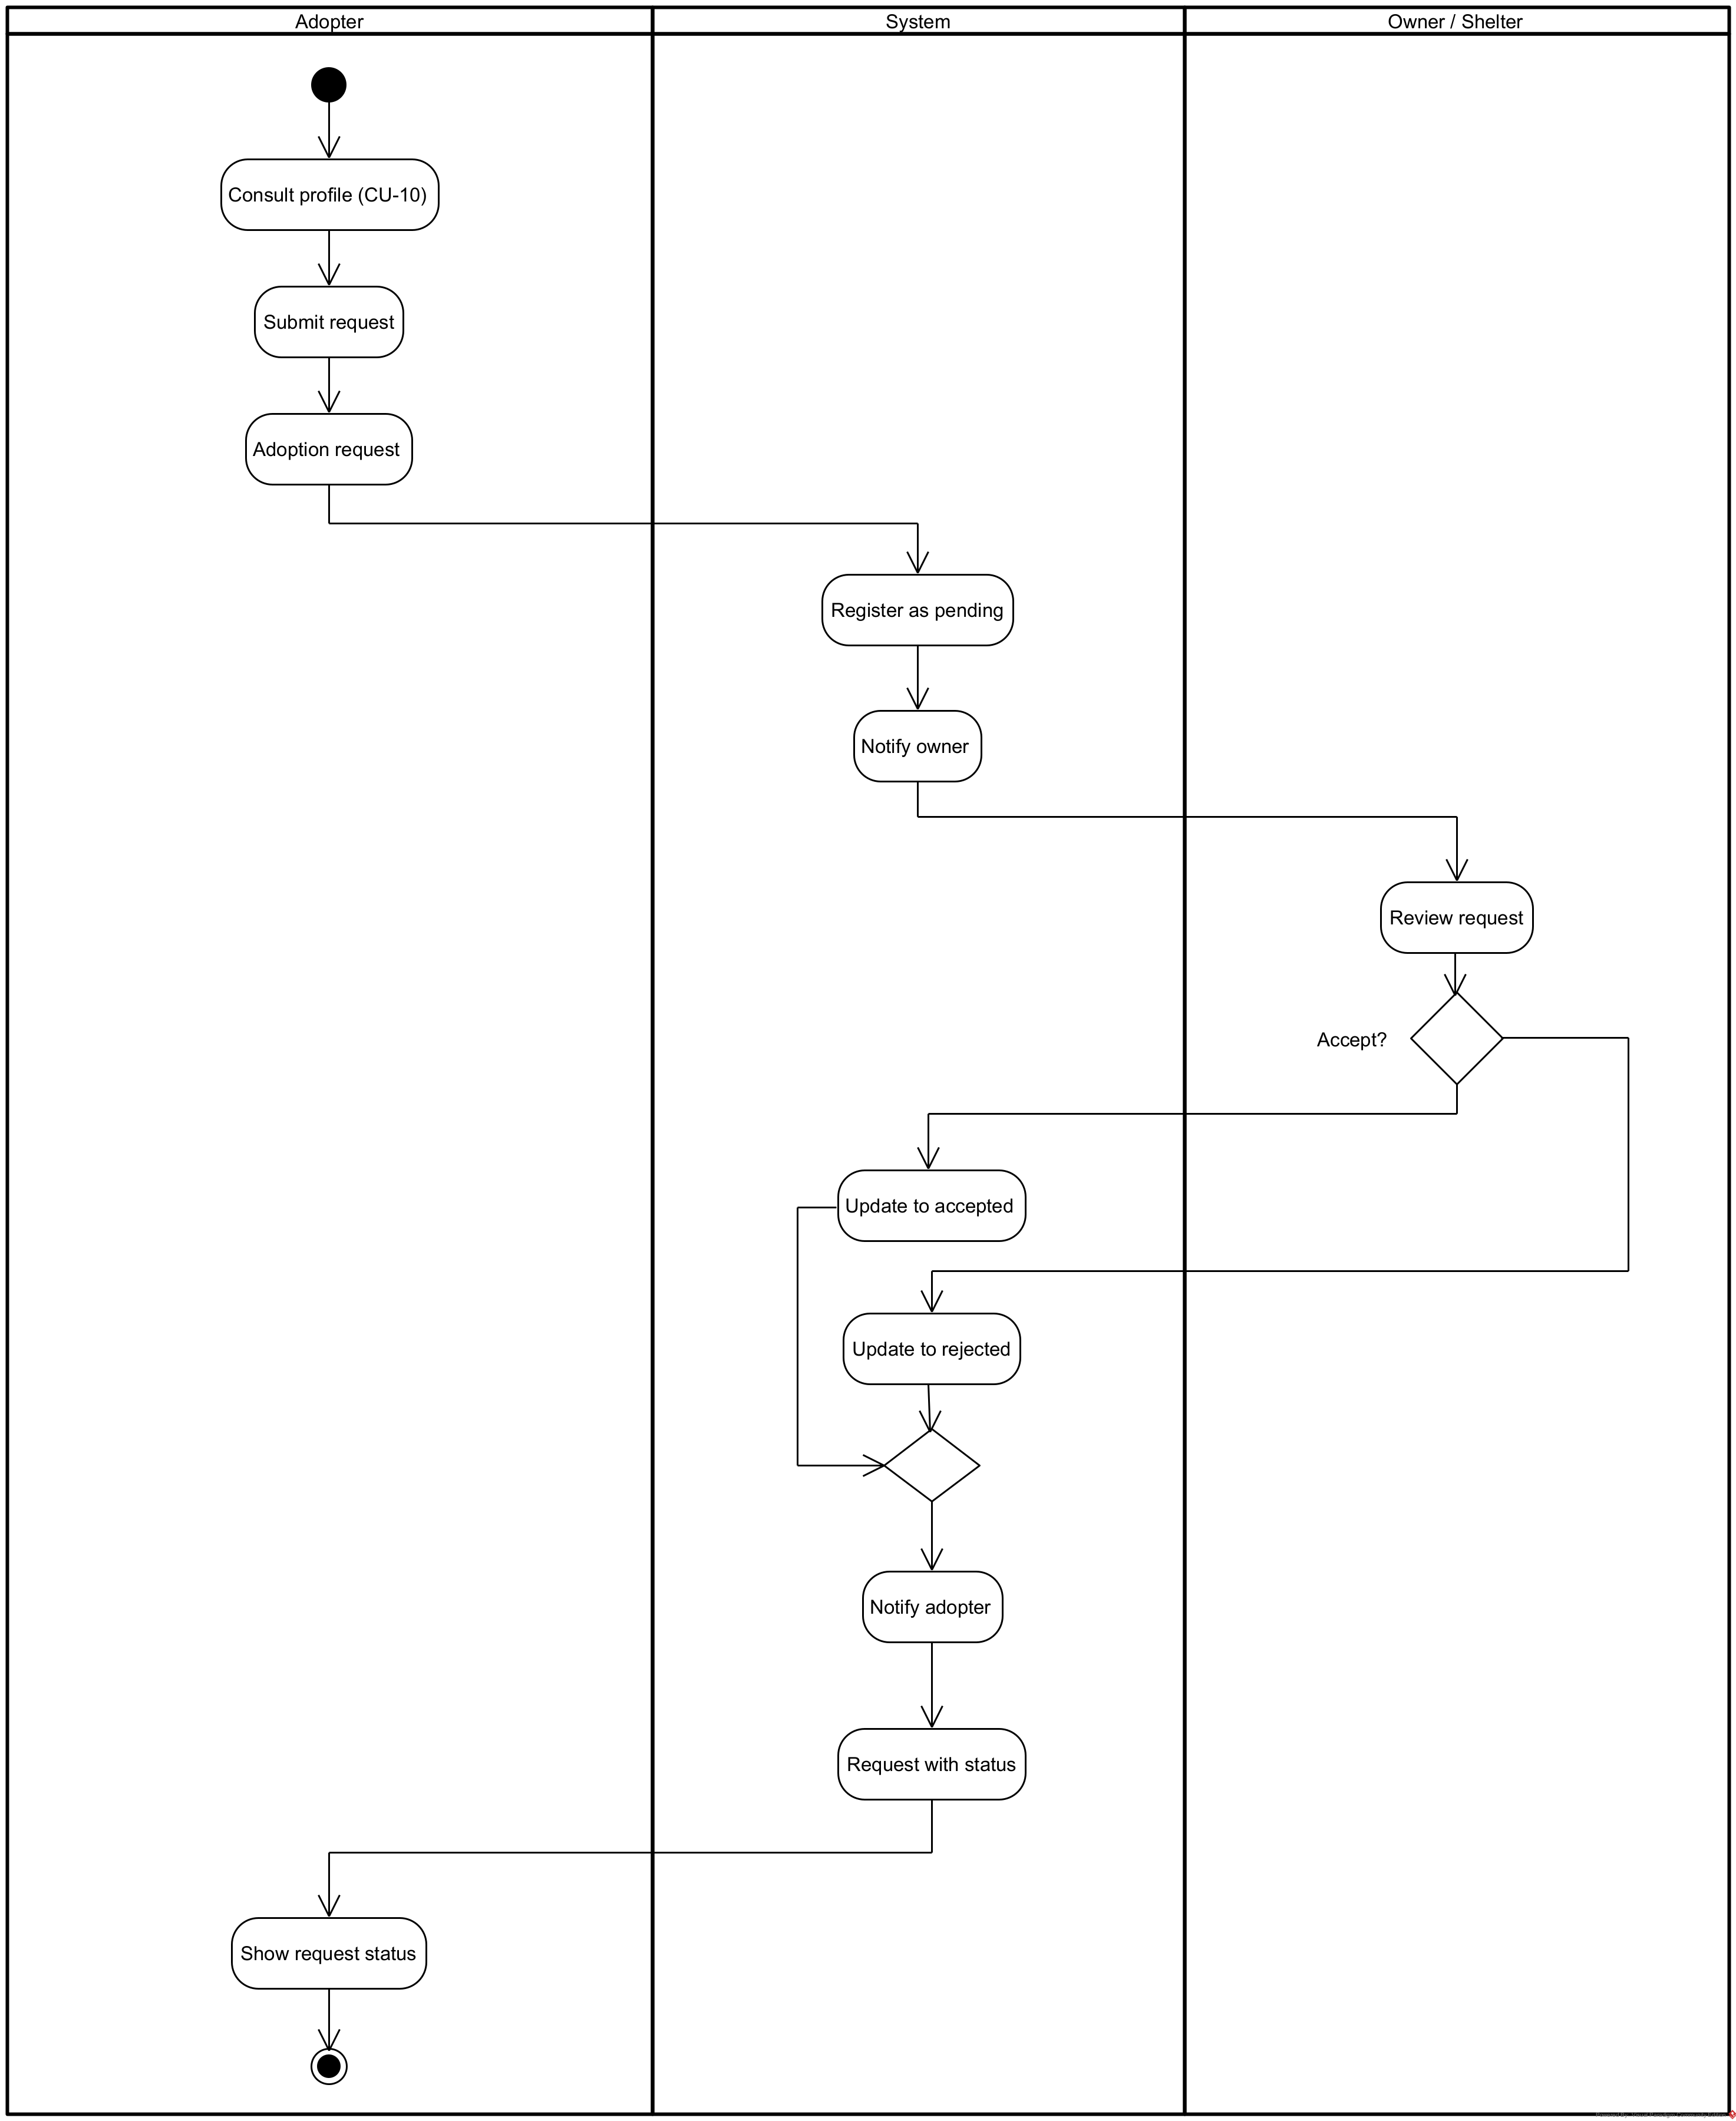
\includegraphics[width=0.82\textwidth]{figuras/DiagramaActividades_CU-07_MundiPets.png}
		\caption{Diagrama de actividad del caso de uso CU-07 --- Consultar historial de procesos de adopción y cruza.}
		\label{fig:act-cu07}
	\end{figure}
	
	\subsubsection{Gestionar comunicación entre usuarios (CU-08)}
	
	El diagrama de actividad de CU-08 detalla el flujo de envío de un mensaje
	entre usuarios (RF-07), incluyendo el paso obligatorio por el componente de
	moderación automática. La bifurcación central determina si el contenido del
	mensaje es apropiado; en caso negativo, el flujo se dirige hacia la
	actividad de notificación de la categoría de infracción detectada y el
	mensaje no llega a entregarse, mientras que en caso afirmativo el mensaje se
	almacena y se notifica al destinatario de forma inmediata.
	
	\begin{figure}[H]
		\centering
		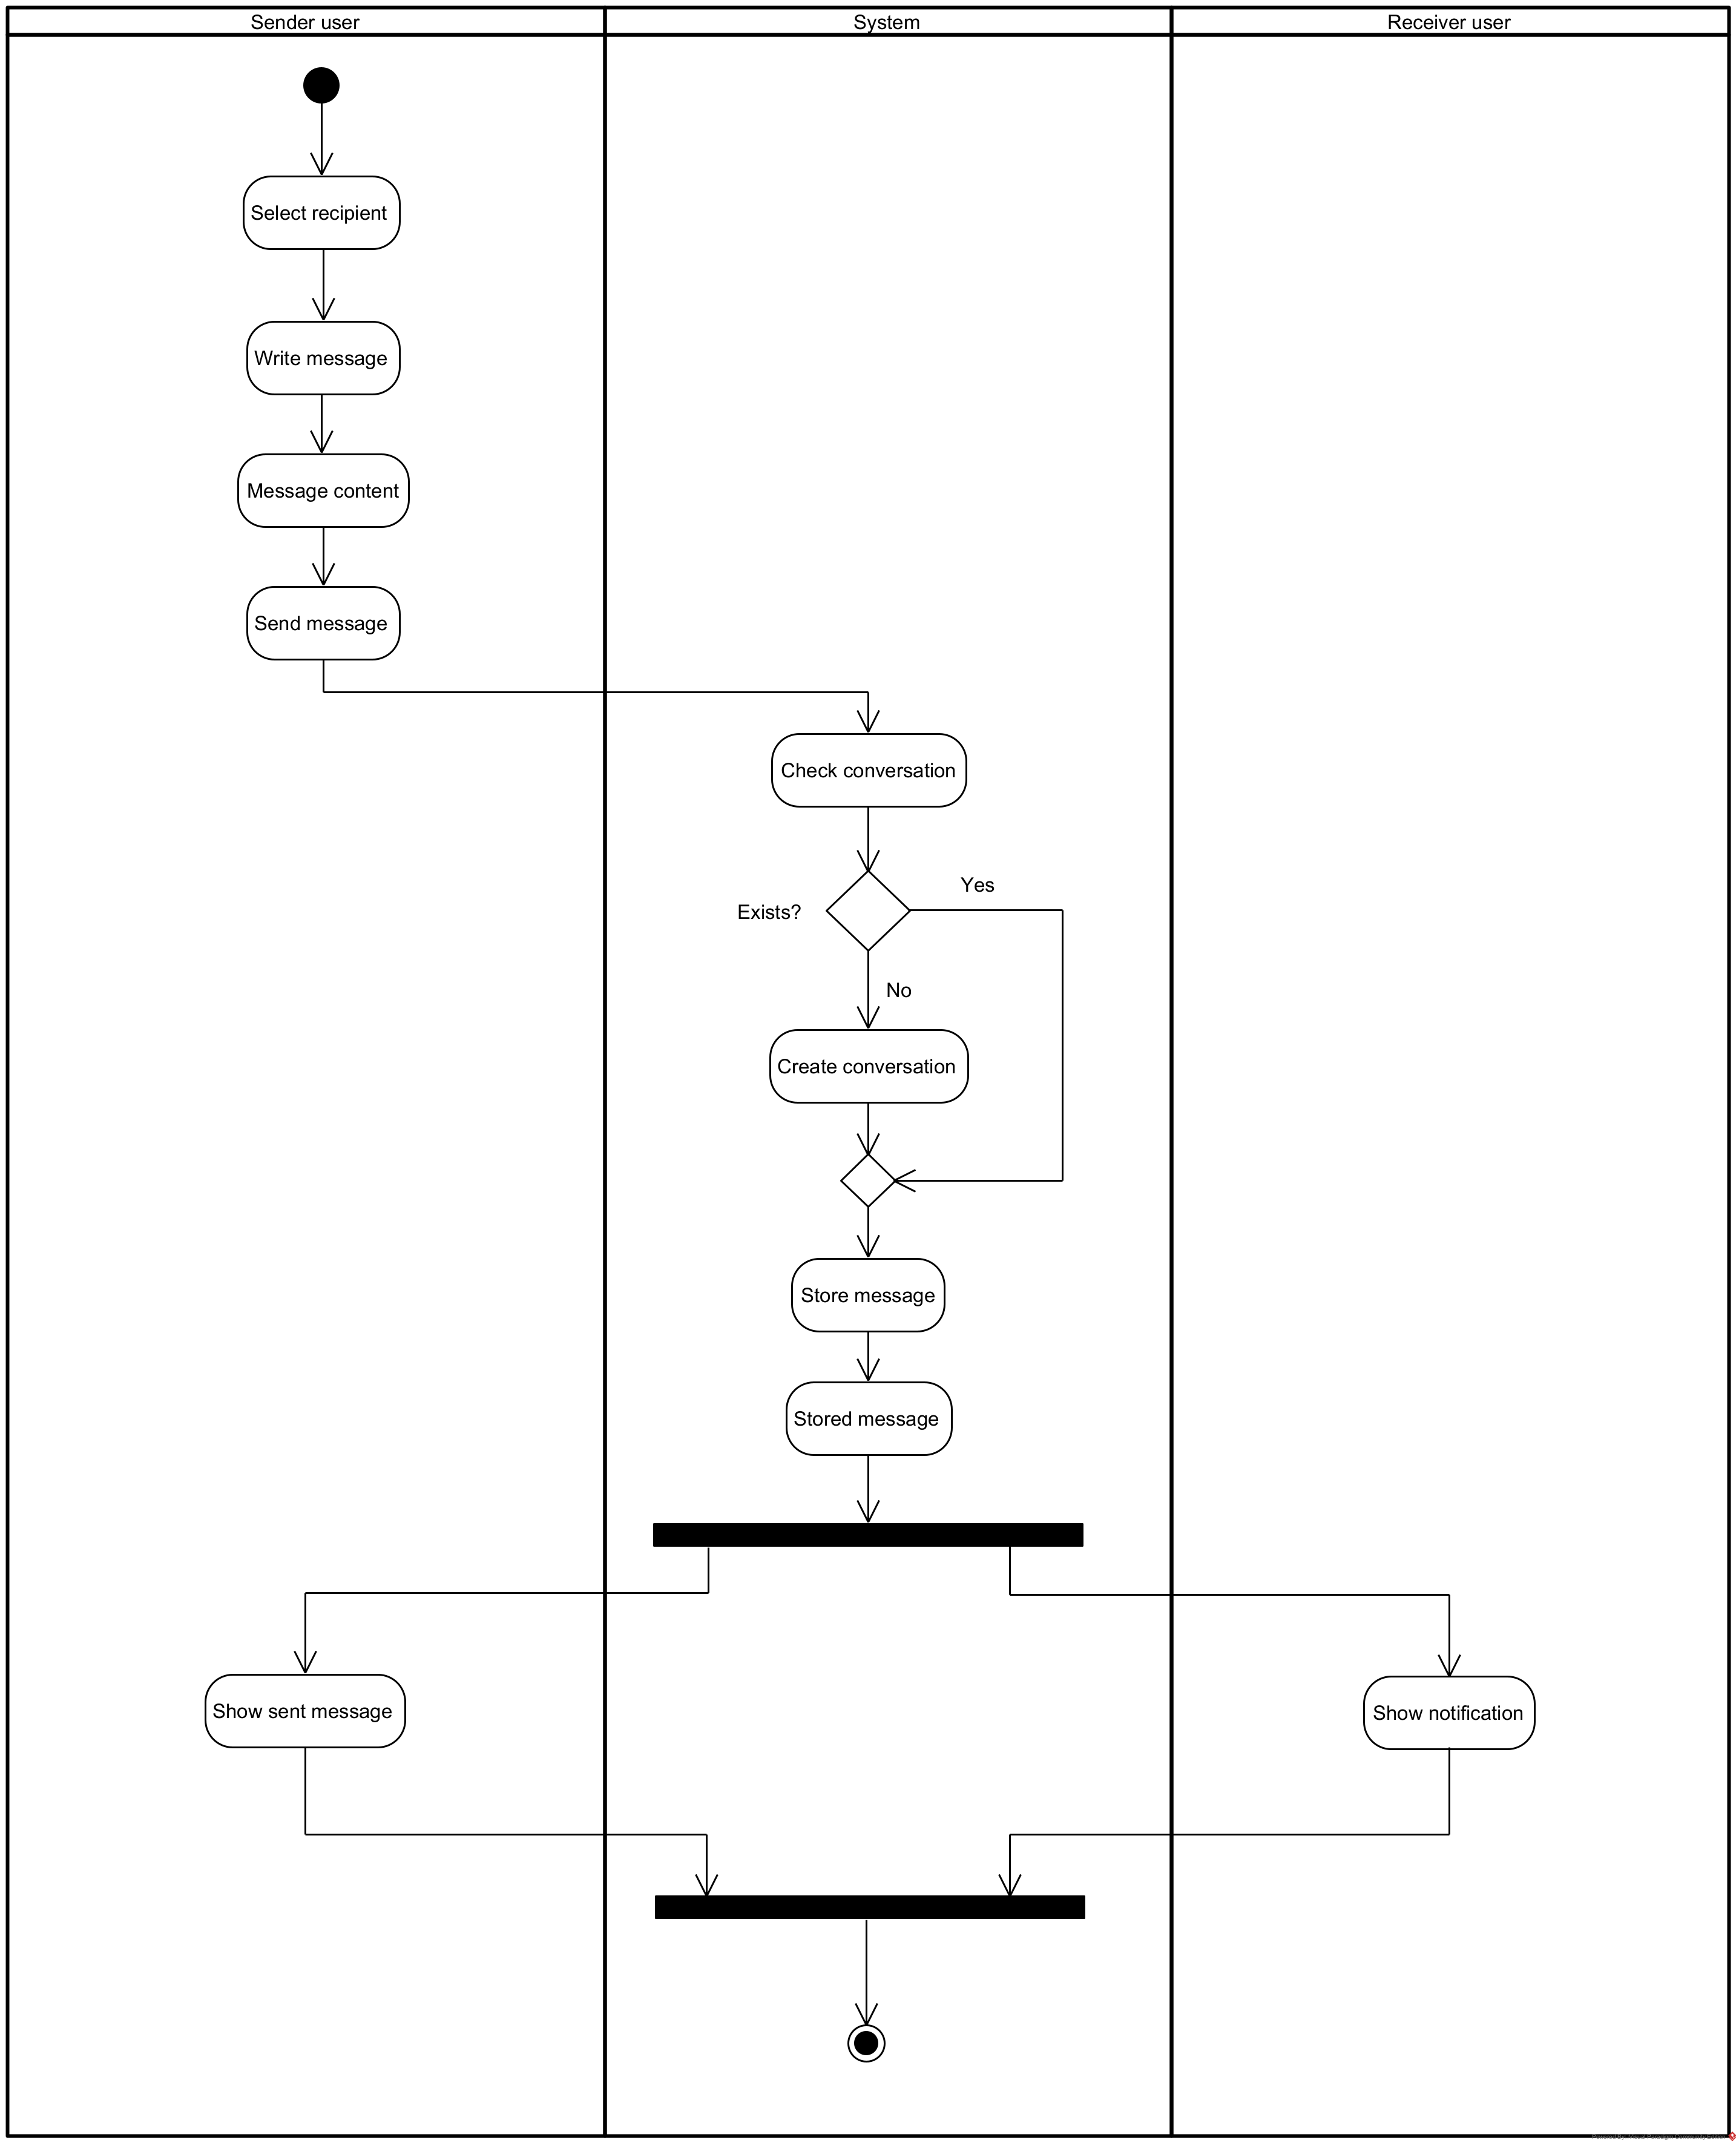
\includegraphics[width=0.81\textwidth]{figuras/DiagramaActividades_CU-08_MundiPets.png}
		\caption{Diagrama de actividad del caso de uso CU-08 --- Gestionar comunicación entre usuarios.}
		\label{fig:act-cu08}
	\end{figure}
	
	\subsubsection{Validar información médica (CU-09)}
	
	Este diagrama representa el flujo de revisión que ejecuta la veterinaria
	sobre el historial médico y los documentos cargados (RF-09). La bifurcación
	principal separa el camino de validación exitosa, que actualiza el estado
	del registro y lo asocia con la identificación del profesional, del camino
	de rechazo, que exige el registro obligatorio de una observación técnica
	antes de notificar al propietario, en coherencia con la máquina de estados
	de verificación de documentos presentada en la
	Sección~\ref{sec:estados}.
	
	\begin{figure}[H]
		\centering
		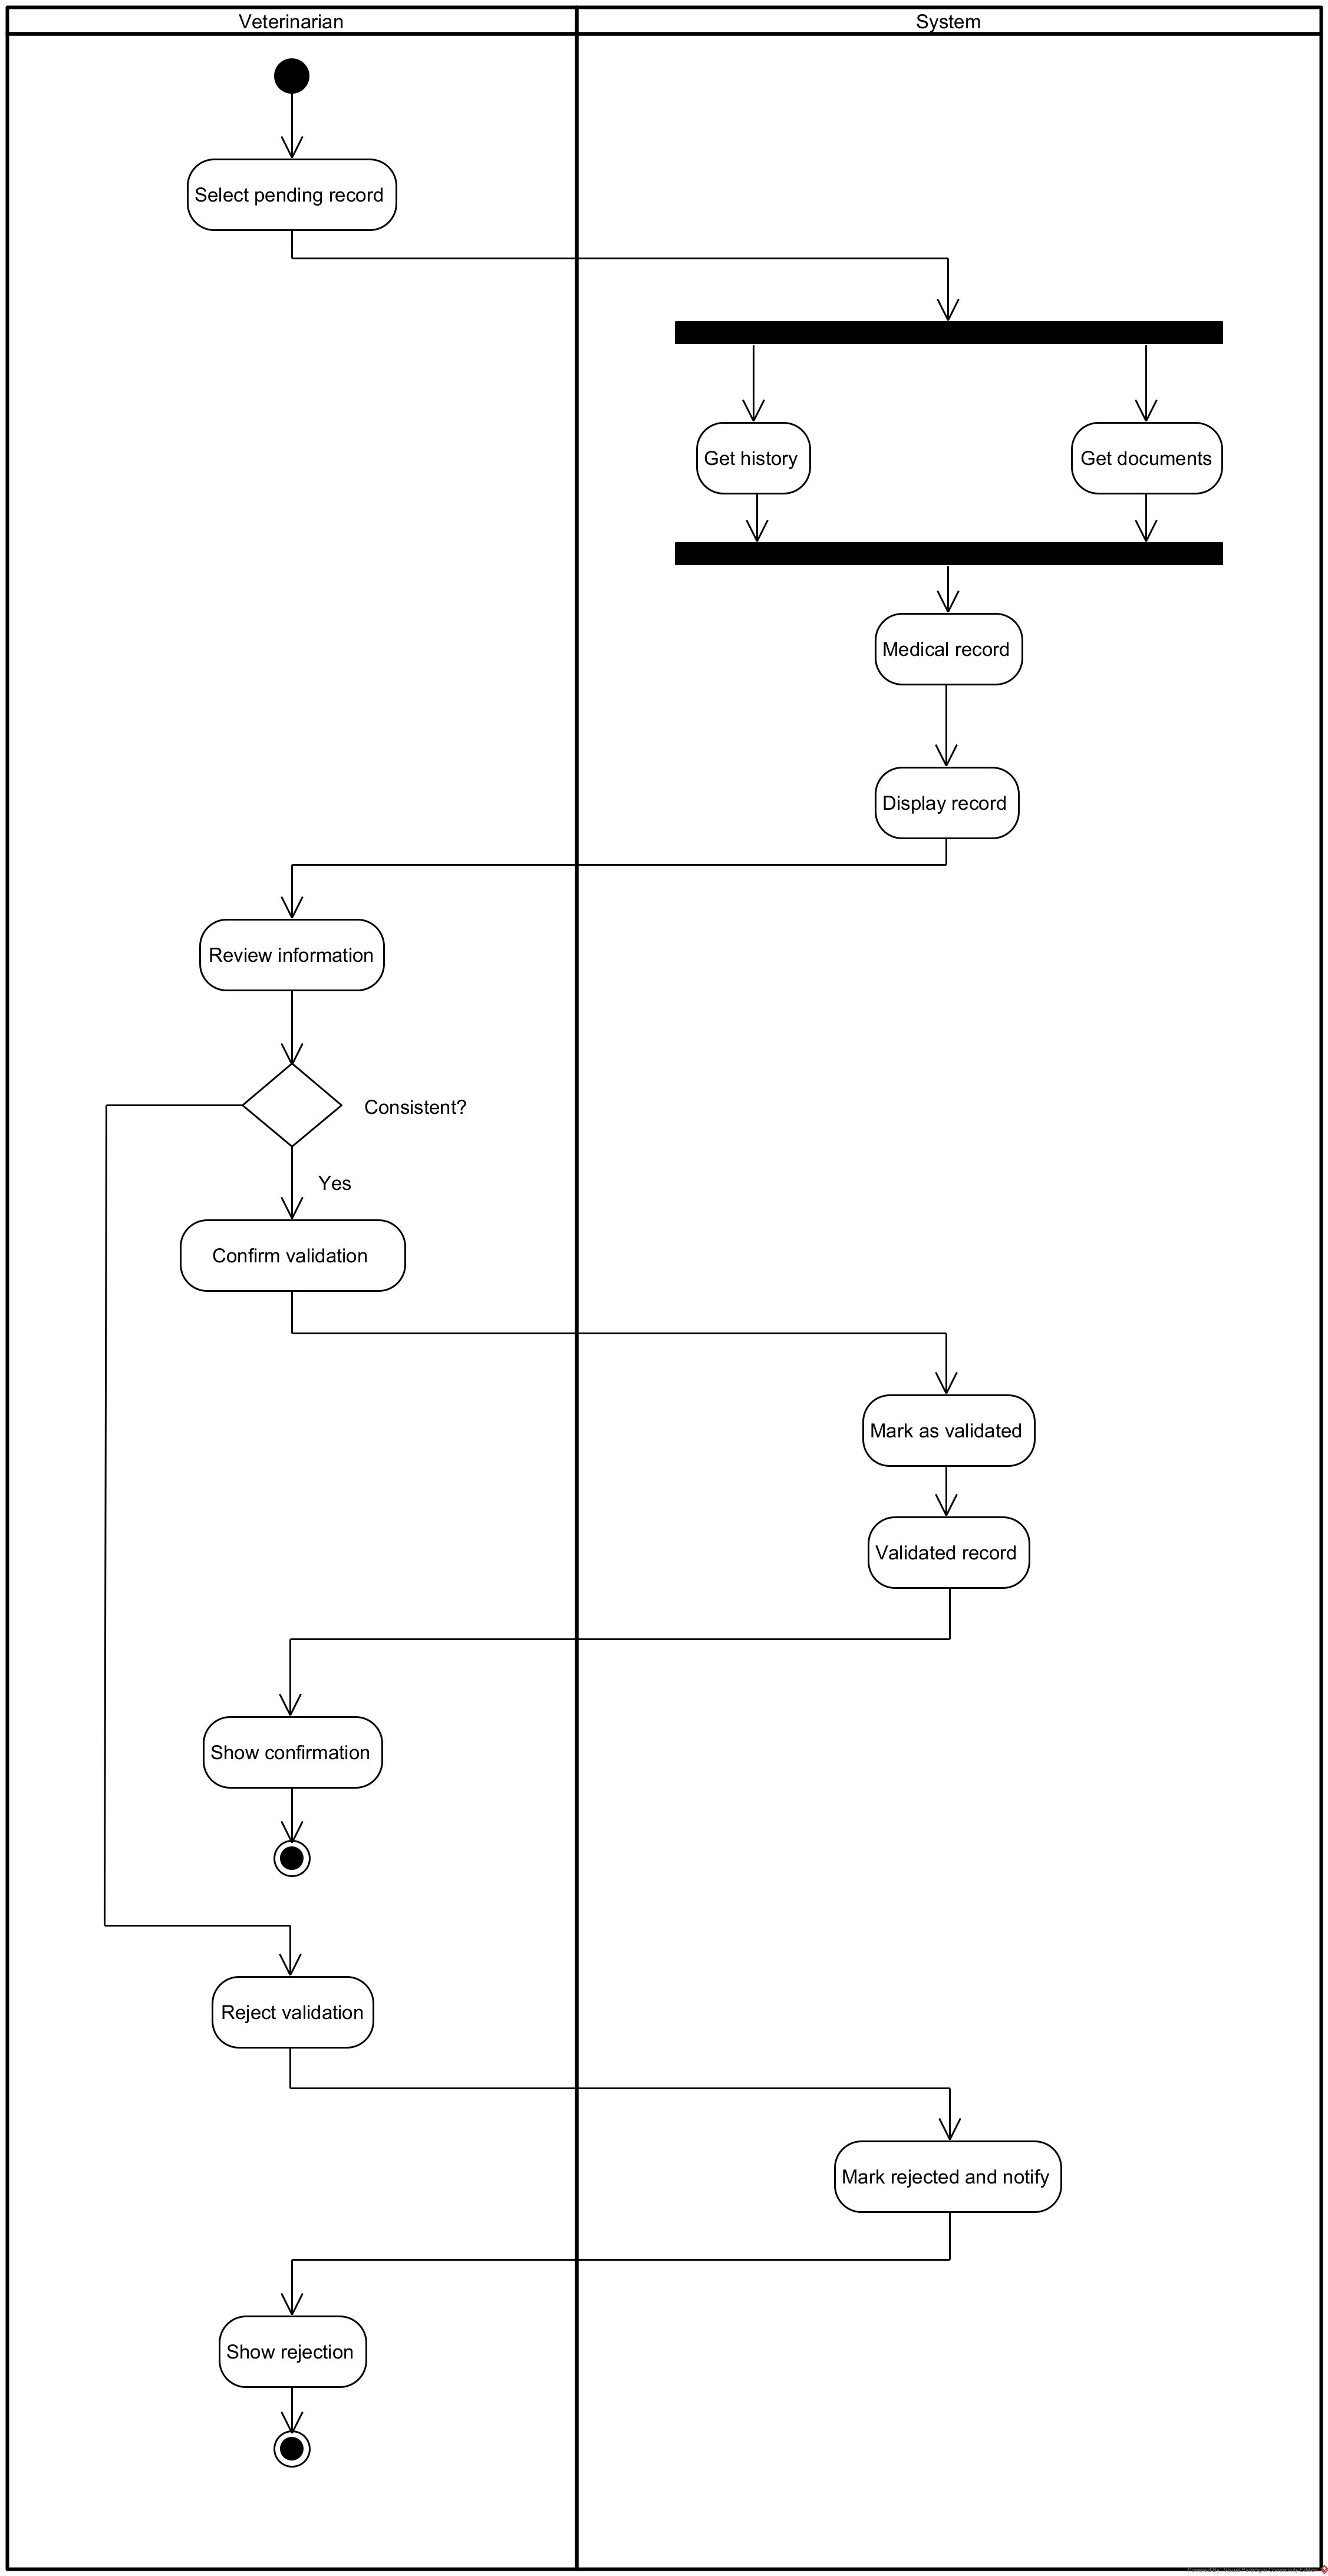
\includegraphics[width=0.52\textwidth]{figuras/DiagramaActividades_CU-09_MundiPets.png}
		\caption{Diagrama de actividad del caso de uso CU-09 --- Validar información médica.}
		\label{fig:act-cu09}
	\end{figure}
	
	\subsubsection{Consultar perfil médico (CU-10)}
	
	El diagrama de actividad de CU-10 expone el flujo de consulta de perfil
	completo de una mascota (RF-03), incluyendo la actividad de filtrado de
	información sensible según el nivel de acceso del usuario consultante y la
	configuración de privacidad definida por el propietario (RF-11). El flujo
	culmina con la presentación diferenciada del perfil, mostrando información
	ampliada a usuarios autorizados y una versión restringida al resto.
	
	\begin{figure}[H]
		\centering
		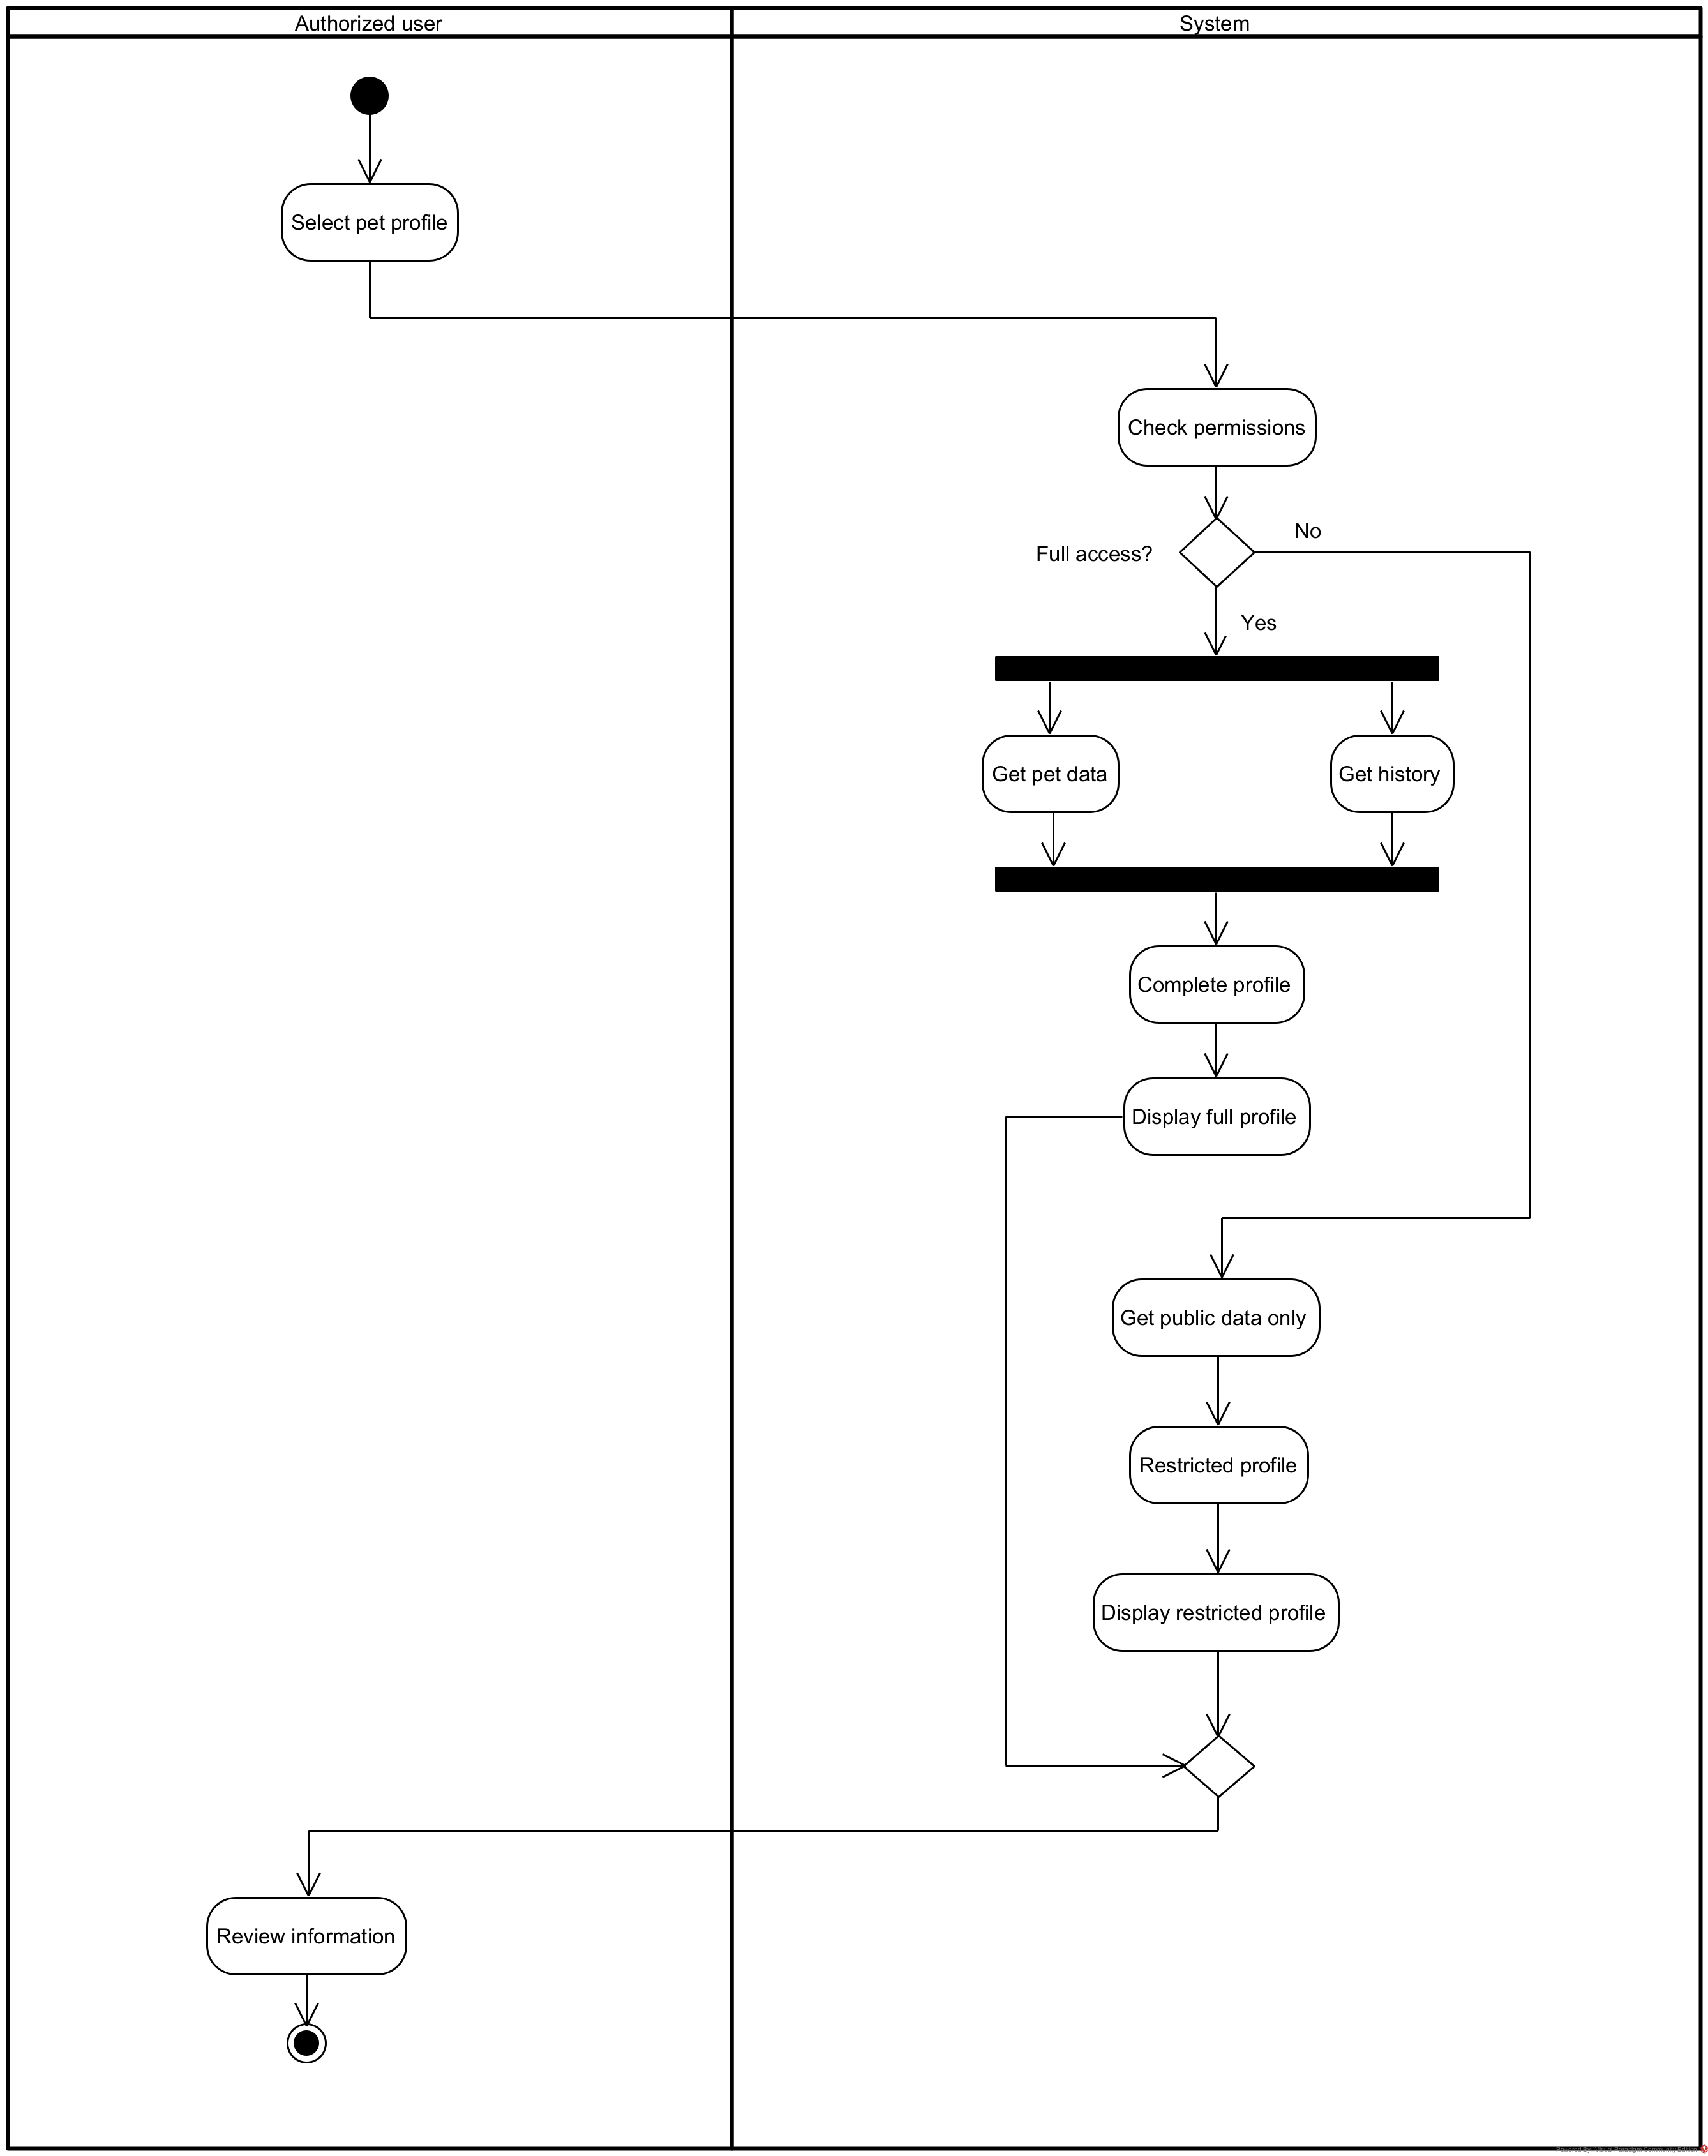
\includegraphics[width=0.80\textwidth]{figuras/DiagramaActividades_CU-10_MundiPets.png}
		\caption{Diagrama de actividad del caso de uso CU-10 --- Consultar perfil médico.}
		\label{fig:act-cu10}
	\end{figure}
	
	\subsubsection{Buscar mascota disponible (CU-11)}
	
	Este diagrama representa el flujo de búsqueda y filtrado de mascotas
	(RF-04). Tras la selección de criterios por parte del usuario, el sistema
	aplica de forma secuencial cada filtro sobre el conjunto de publicaciones
	activas y evalúa si existen resultados; en caso de no existir coincidencias,
	el flujo ofrece al usuario ajustar los criterios antes de repetir la
	búsqueda, evitando presentar una lista vacía sin alternativas de acción.
	
	\begin{figure}[H]
		\centering
		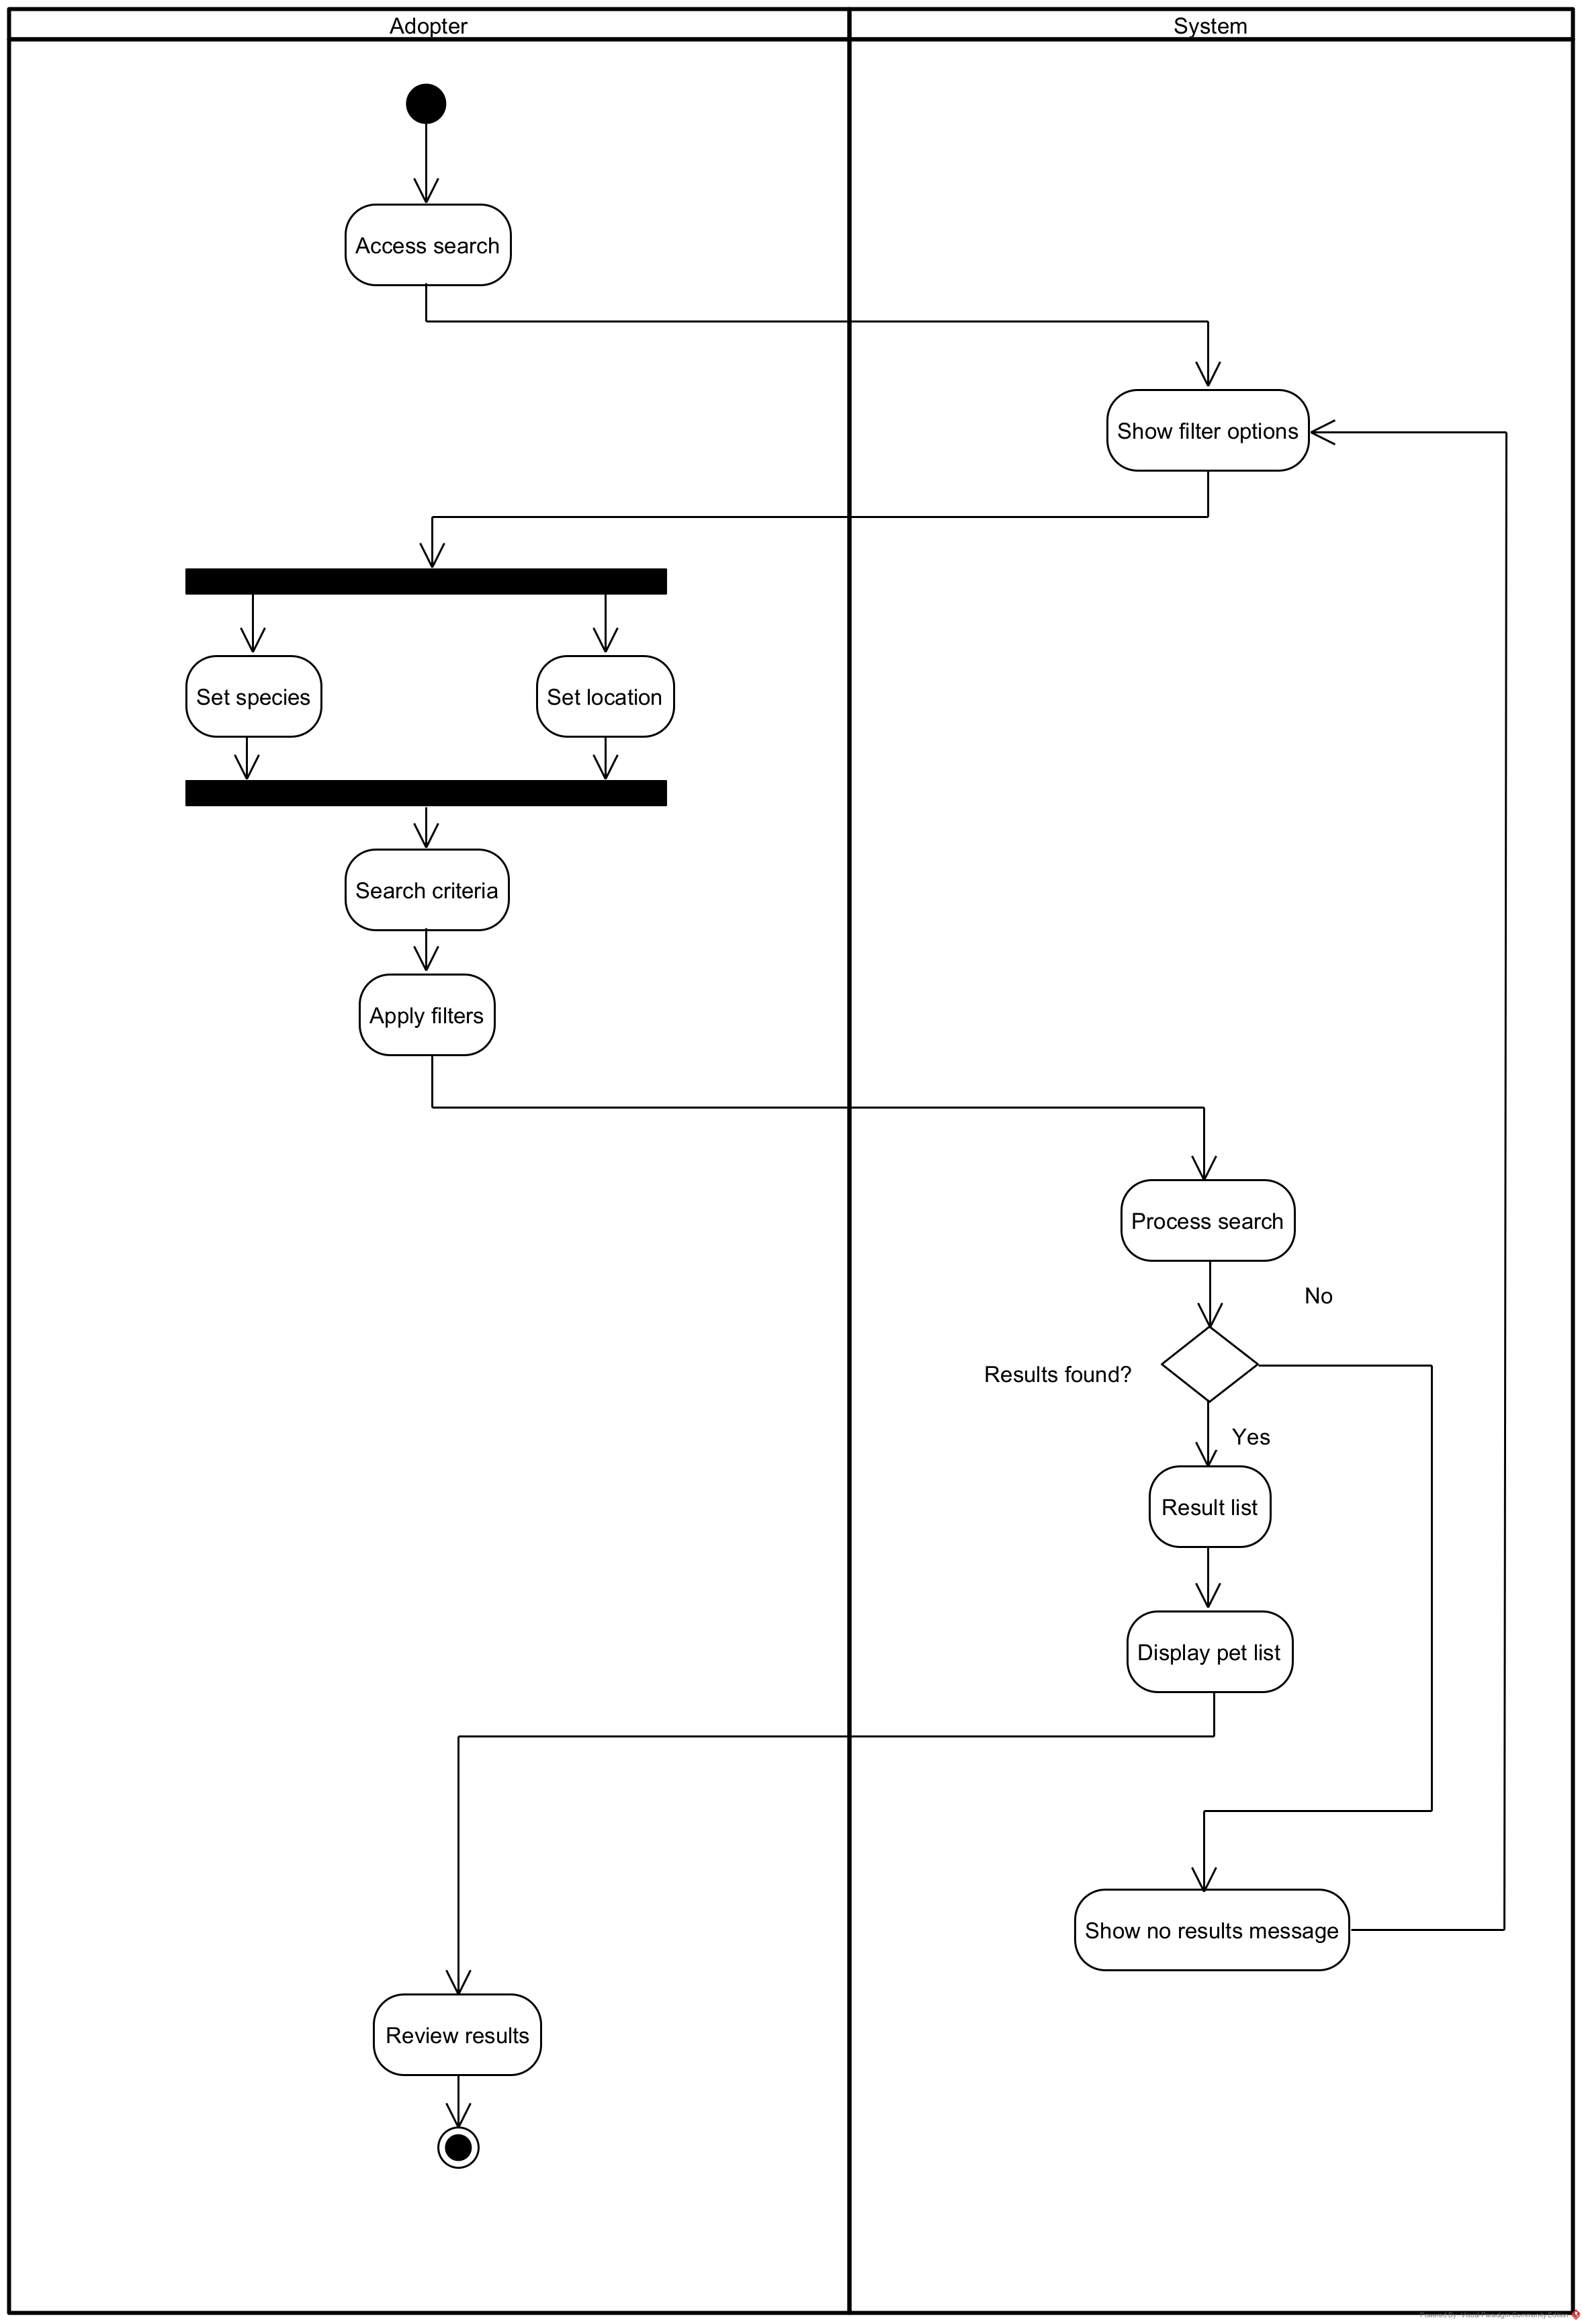
\includegraphics[width=0.73\textwidth]{figuras/DiagramaActividades_CU-11_MundiPets.png}
		\caption{Diagrama de actividad del caso de uso CU-11 --- Buscar mascota disponible.}
		\label{fig:act-cu11}
	\end{figure}
	
	\subsubsection{Configurar privacidad médica (CU-12)}
	
	El diagrama de actividad de CU-12 detalla el flujo de configuración de
	privacidad (RF-11). La bifurcación central verifica si alguno de los campos
	que el propietario intenta restringir es un campo médico obligatorio para la
	validación veterinaria; si lo es, el sistema muestra una advertencia y no
	aplica la restricción sobre ese campo específico, mientras que el resto de
	la configuración se guarda con normalidad, permitiendo un ajuste parcial en
	lugar de rechazar la operación completa.
	
	\begin{figure}[H]
		\centering
		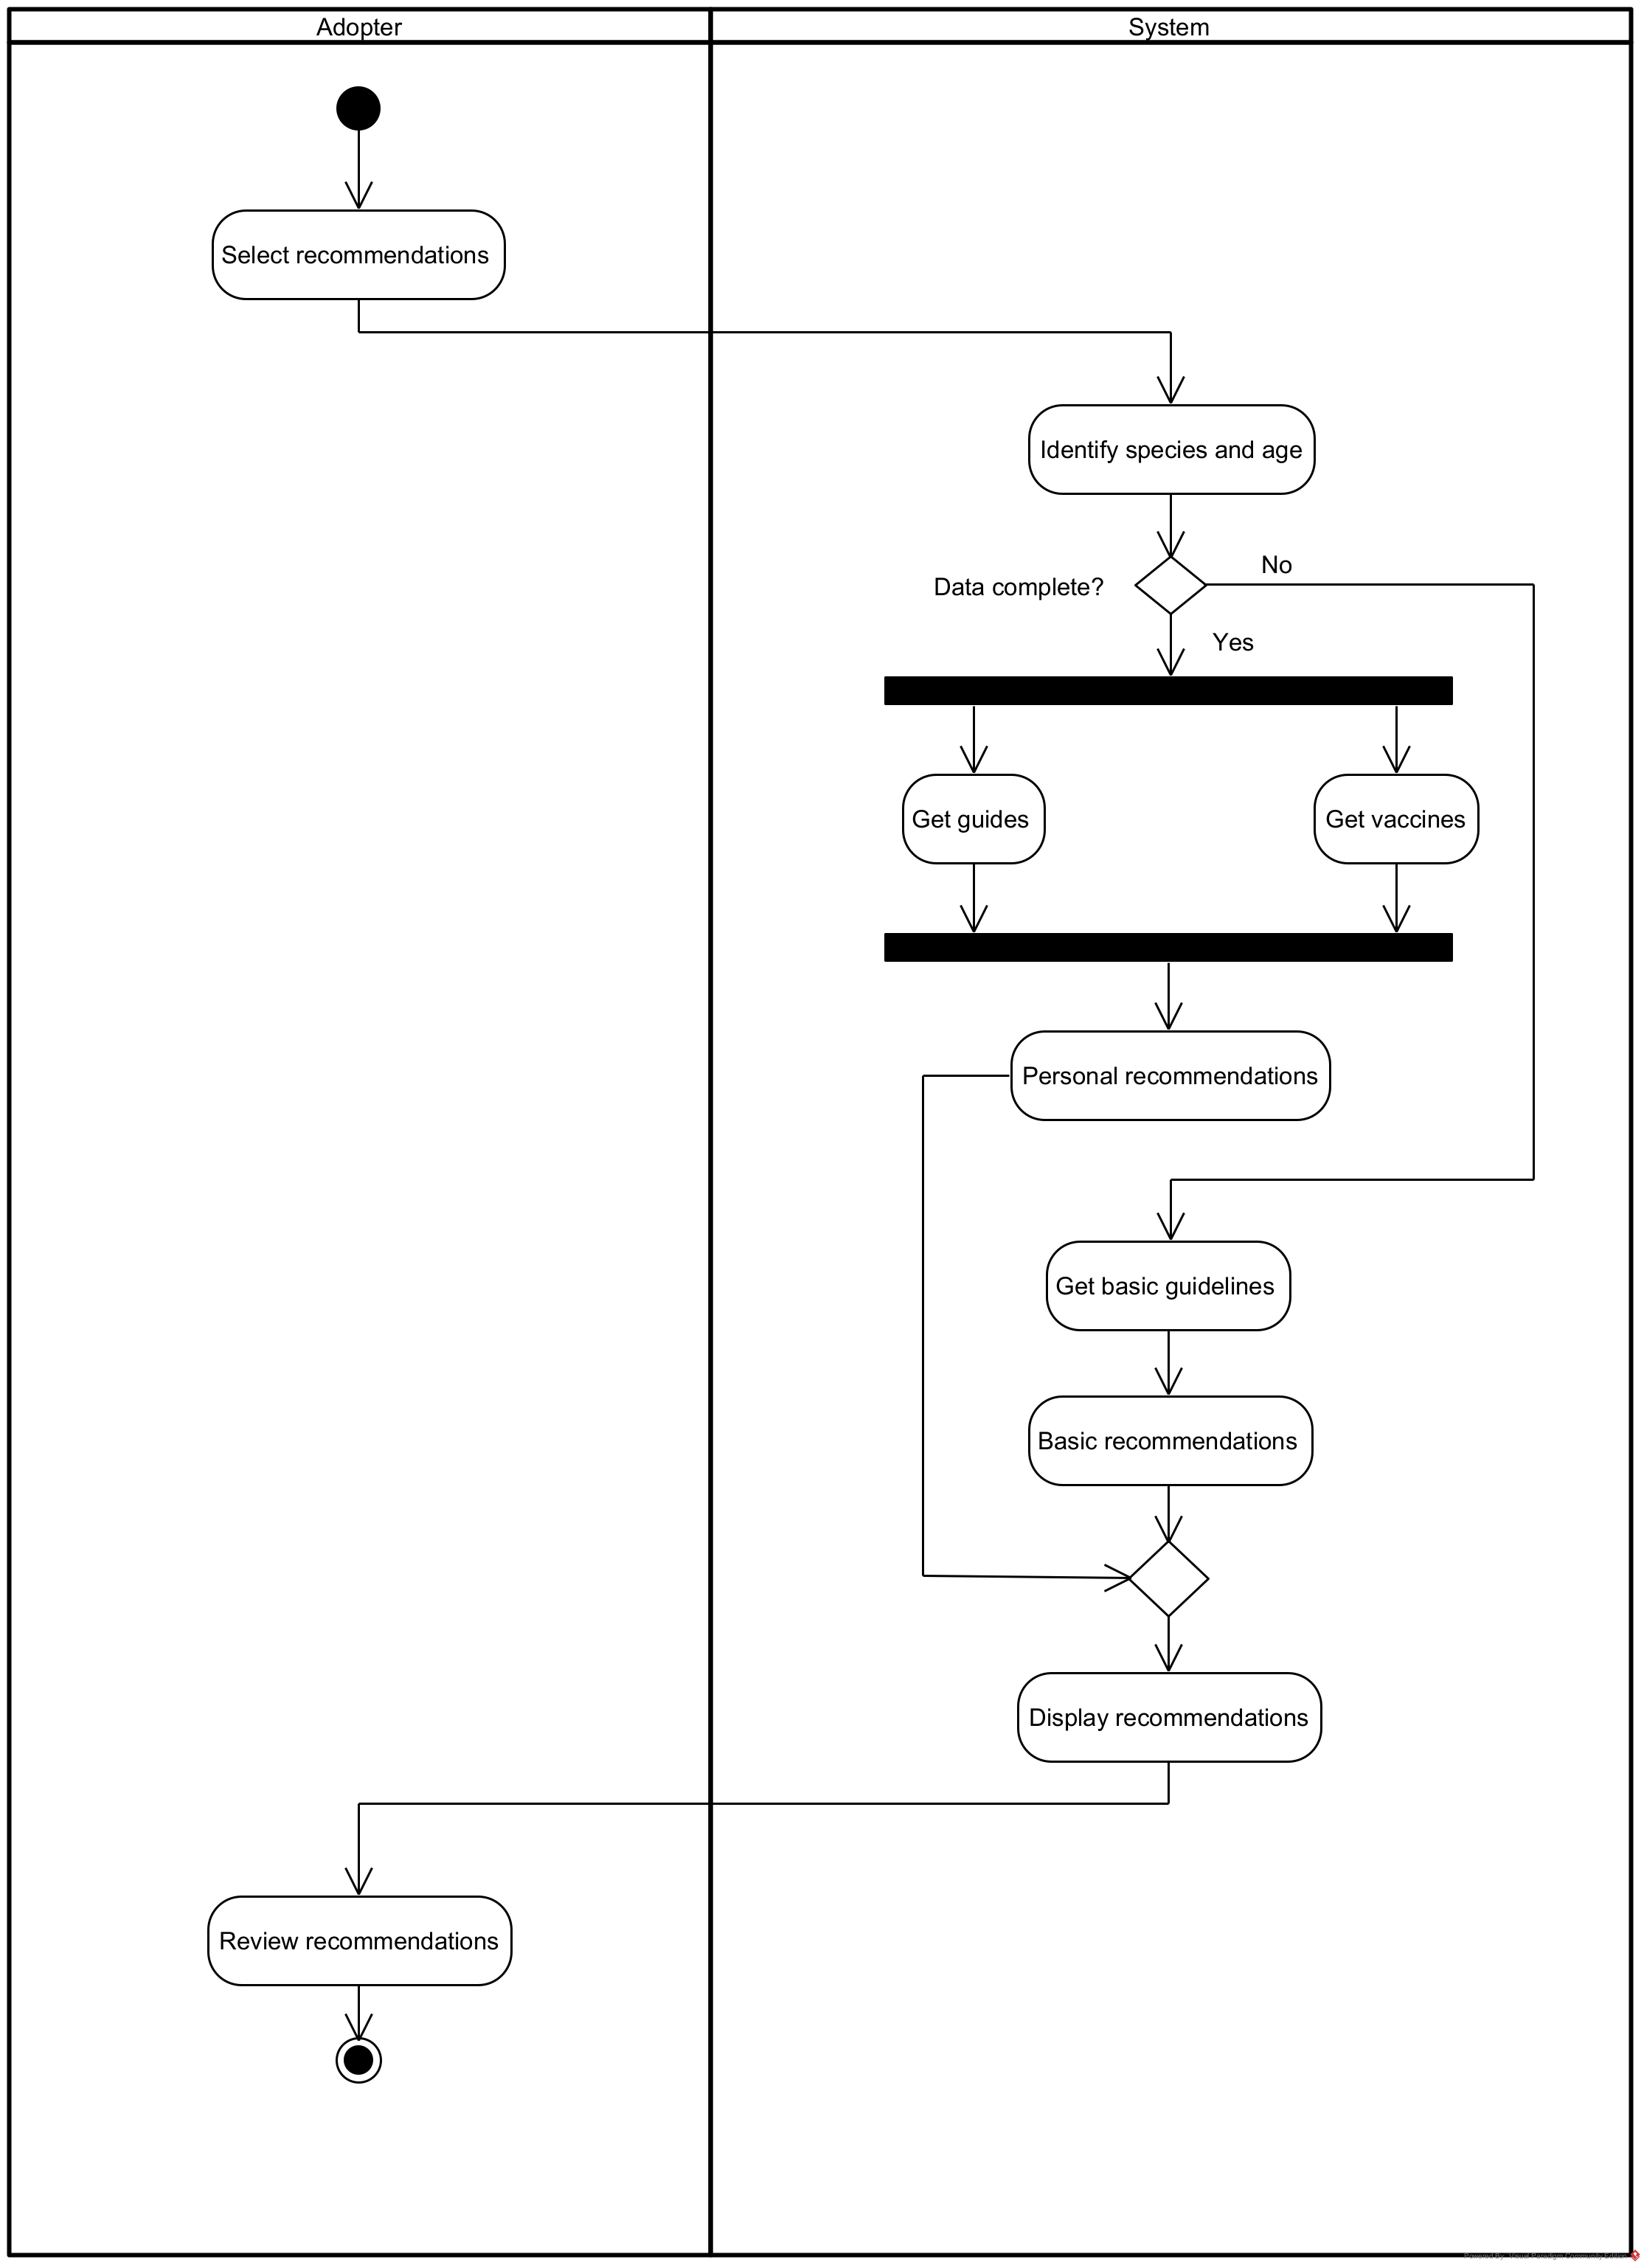
\includegraphics[width=0.73\textwidth]{figuras/DiagramaActividades_CU-12_MundiPets.png}
		\caption{Diagrama de actividad del caso de uso CU-12 --- Configurar privacidad médica.}
		\label{fig:act-cu12}
	\end{figure}
	
	\subsubsection{Evaluar compatibilidad de cruza --- verificación de parentesco (CU-13)}
	
	Este diagrama detalla el flujo de verificación de parentesco previo a la
	evaluación de compatibilidad (RF-06, RF-16). La actividad central compara el
	linaje declarado de ambas mascotas antes de invocar el componente de
	inteligencia artificial; si detecta un grado de parentesco incompatible, el
	flujo se dirige directamente hacia la actividad de alerta explícita y
	finaliza sin generar una recomendación de compatibilidad, evitando así que
	el sistema sugiera una cruza que la propia especificación textual del caso
	de uso (flujo alterno 3.1 de la Tabla~\ref{tab:CU-13}) considera inviable.
	
	\begin{figure}[H]
		\centering
		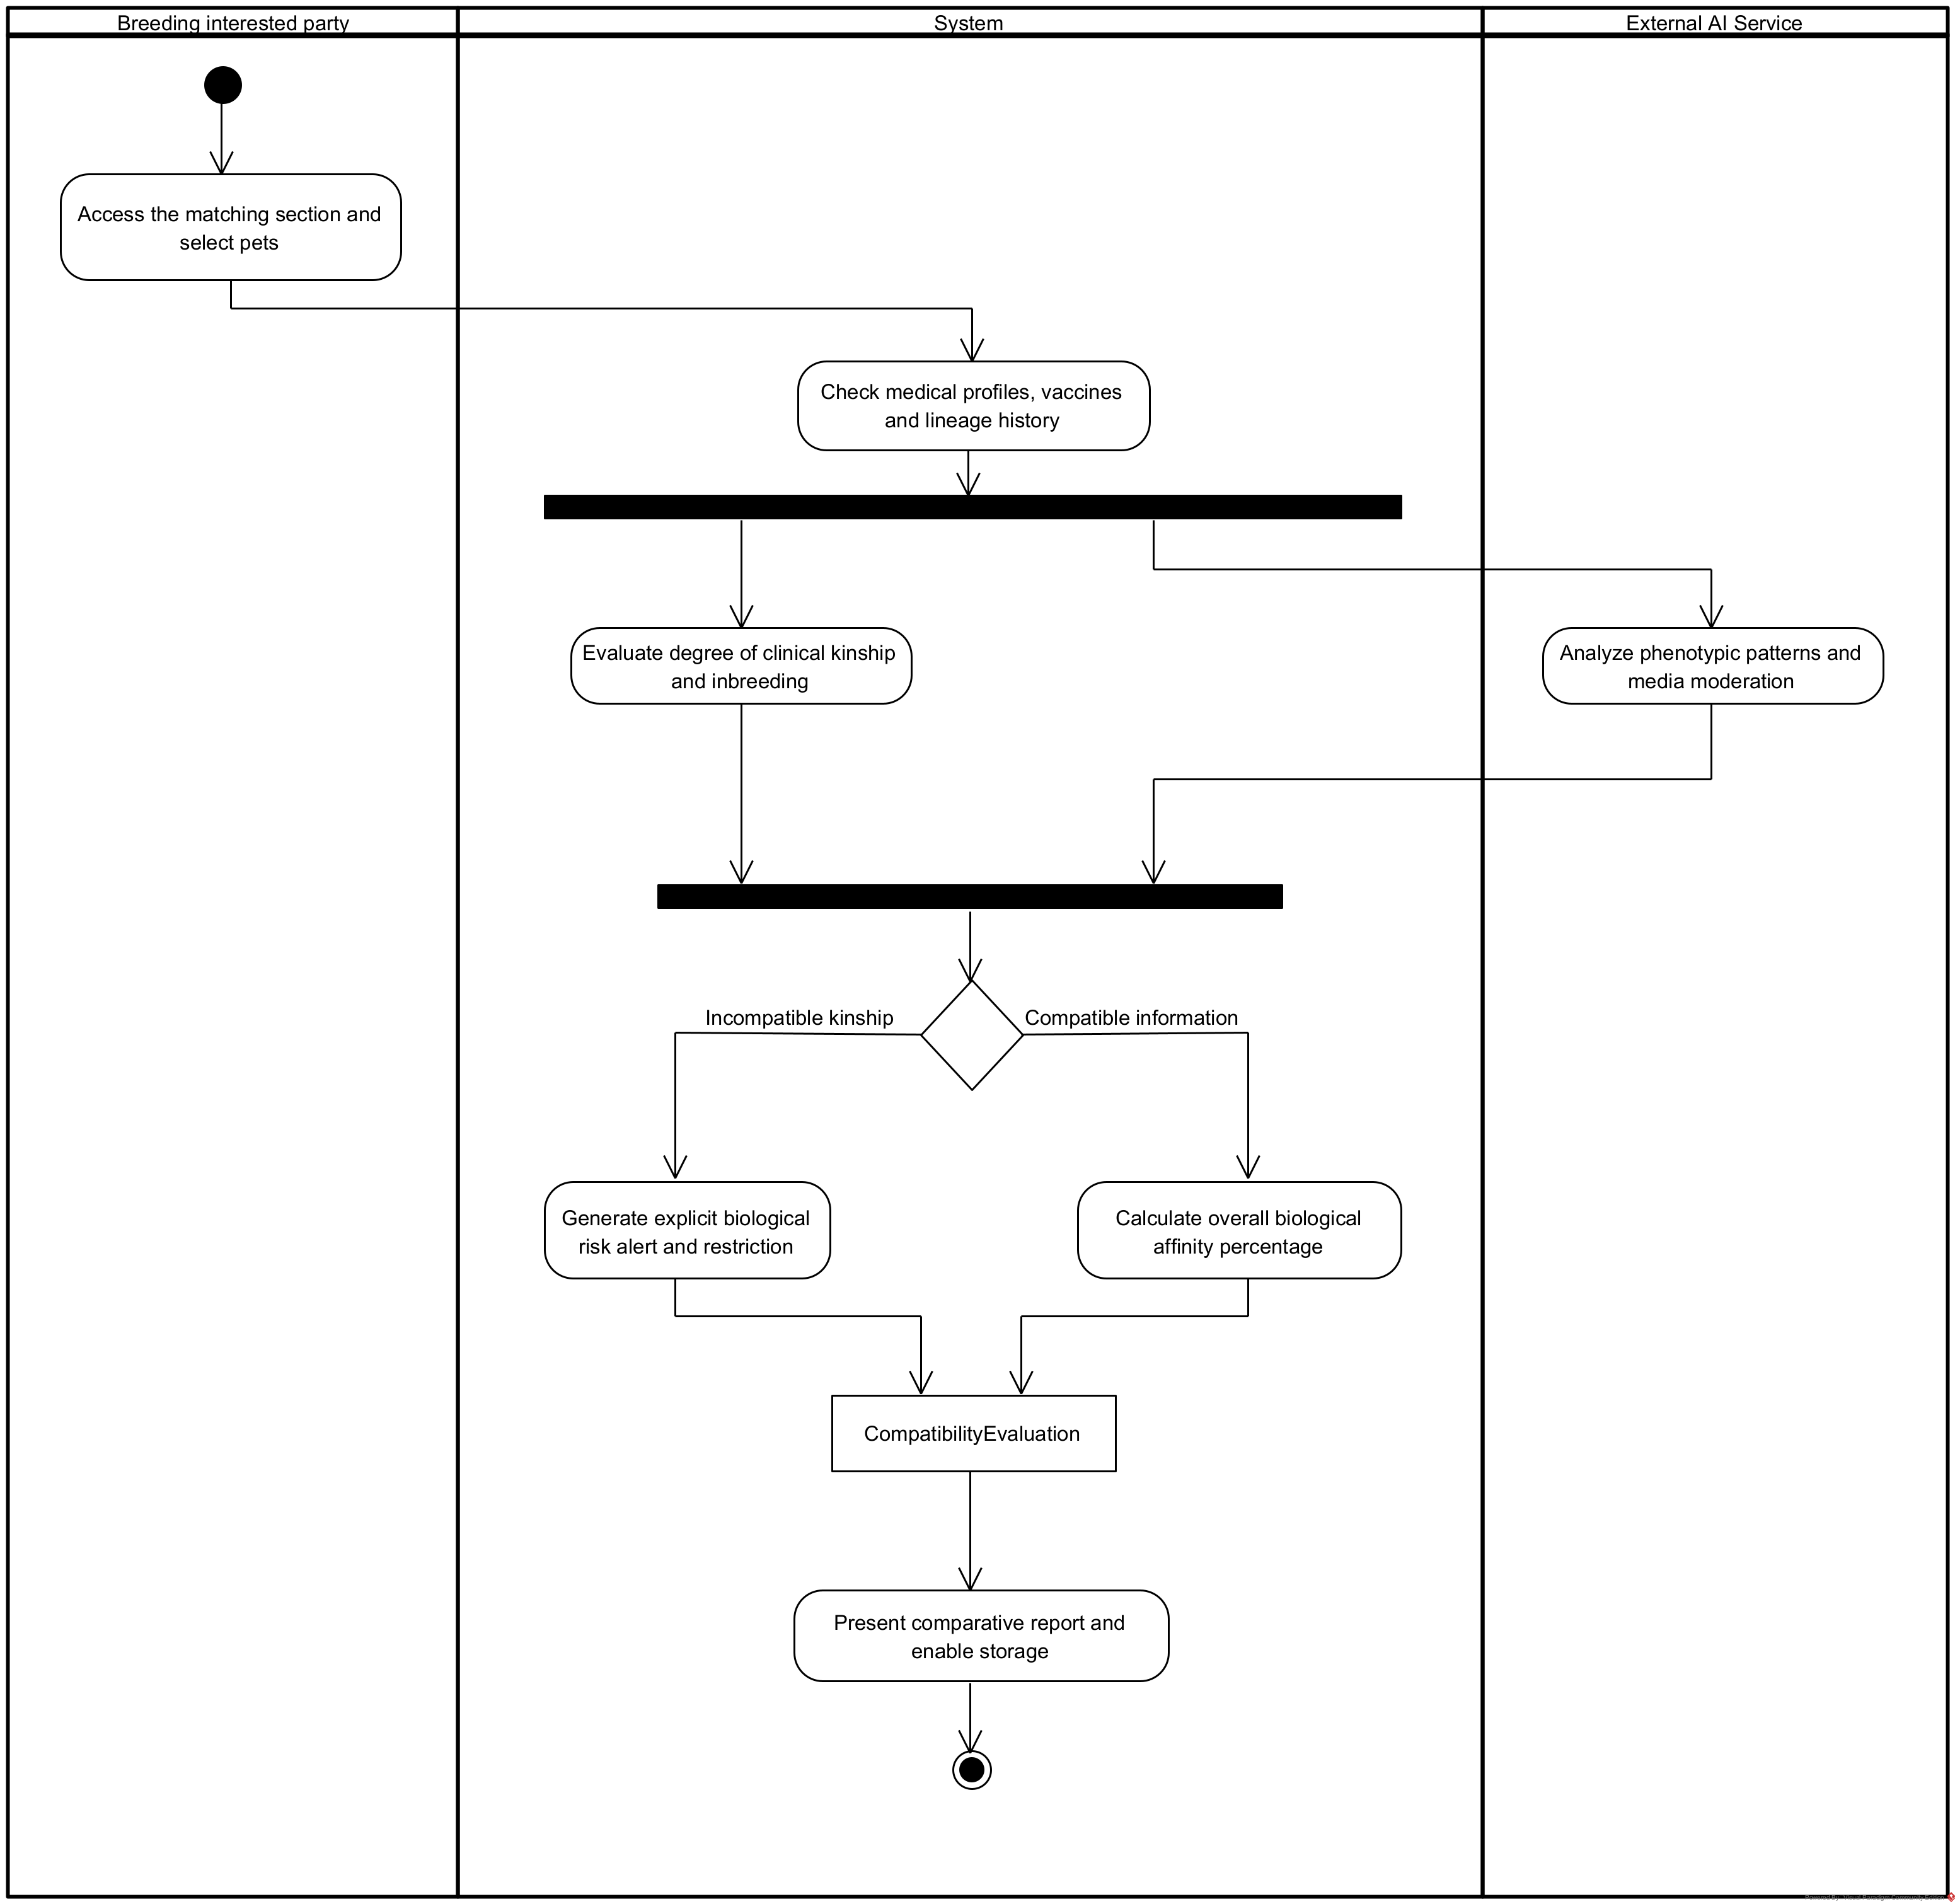
\includegraphics[width=1\textwidth]{figuras/DiagramaActividades_CU-13_MundiPets.png}
		\caption{Diagrama de actividad del caso de uso CU-13 --- Verificación de parentesco previa a la evaluación de compatibilidad.}
		\label{fig:act-cu13}
	\end{figure}
	
	% ------------------------------------------------------------
	\subsection{Diagrama de estados}
	\label{sec:estados}
	
	Se modelan tres máquinas de estado correspondientes a las entidades del
	sistema cuyo comportamiento depende fuertemente de transiciones bien
	definidas: el perfil de una mascota, una solicitud de adopción o cruza, y el
	proceso de verificación de documentos médicos. Estas tres entidades
	concentran la mayor parte de la lógica de negocio condicionada por el rol
	del usuario y por las validaciones cruzadas entre propietarios, adoptantes y
	veterinarias.
	
	\subsubsection{Estados del perfil de mascota}
	
	El ciclo de vida del perfil de una mascota inicia en el estado
	\emph{Registrada} una vez completado RF-01, y transita hacia
	\emph{Publicada} cuando el propietario habilita su disponibilidad para
	adopción o cruza (RF-13). Desde este estado puede alcanzar
	\emph{Verificada} cuando una veterinaria valida su información médica
	(RF-09), o bien \emph{EnProcesoDeAdopcion} / \emph{EnProcesoDeCruza} al
	aceptarse una solicitud. El estado \emph{Adoptada} es final para el flujo de
	adopción, pero habilita la transición hacia \emph{EnSeguimiento} definida
	por RF-22, mientras que el estado \emph{Extraviada}, alcanzable desde
	cualquier estado activo mediante RF-25, retorna a \emph{Publicada} una vez
	que el propietario marca el aviso como resuelto.
	
	\begin{figure}[H]
		\centering
		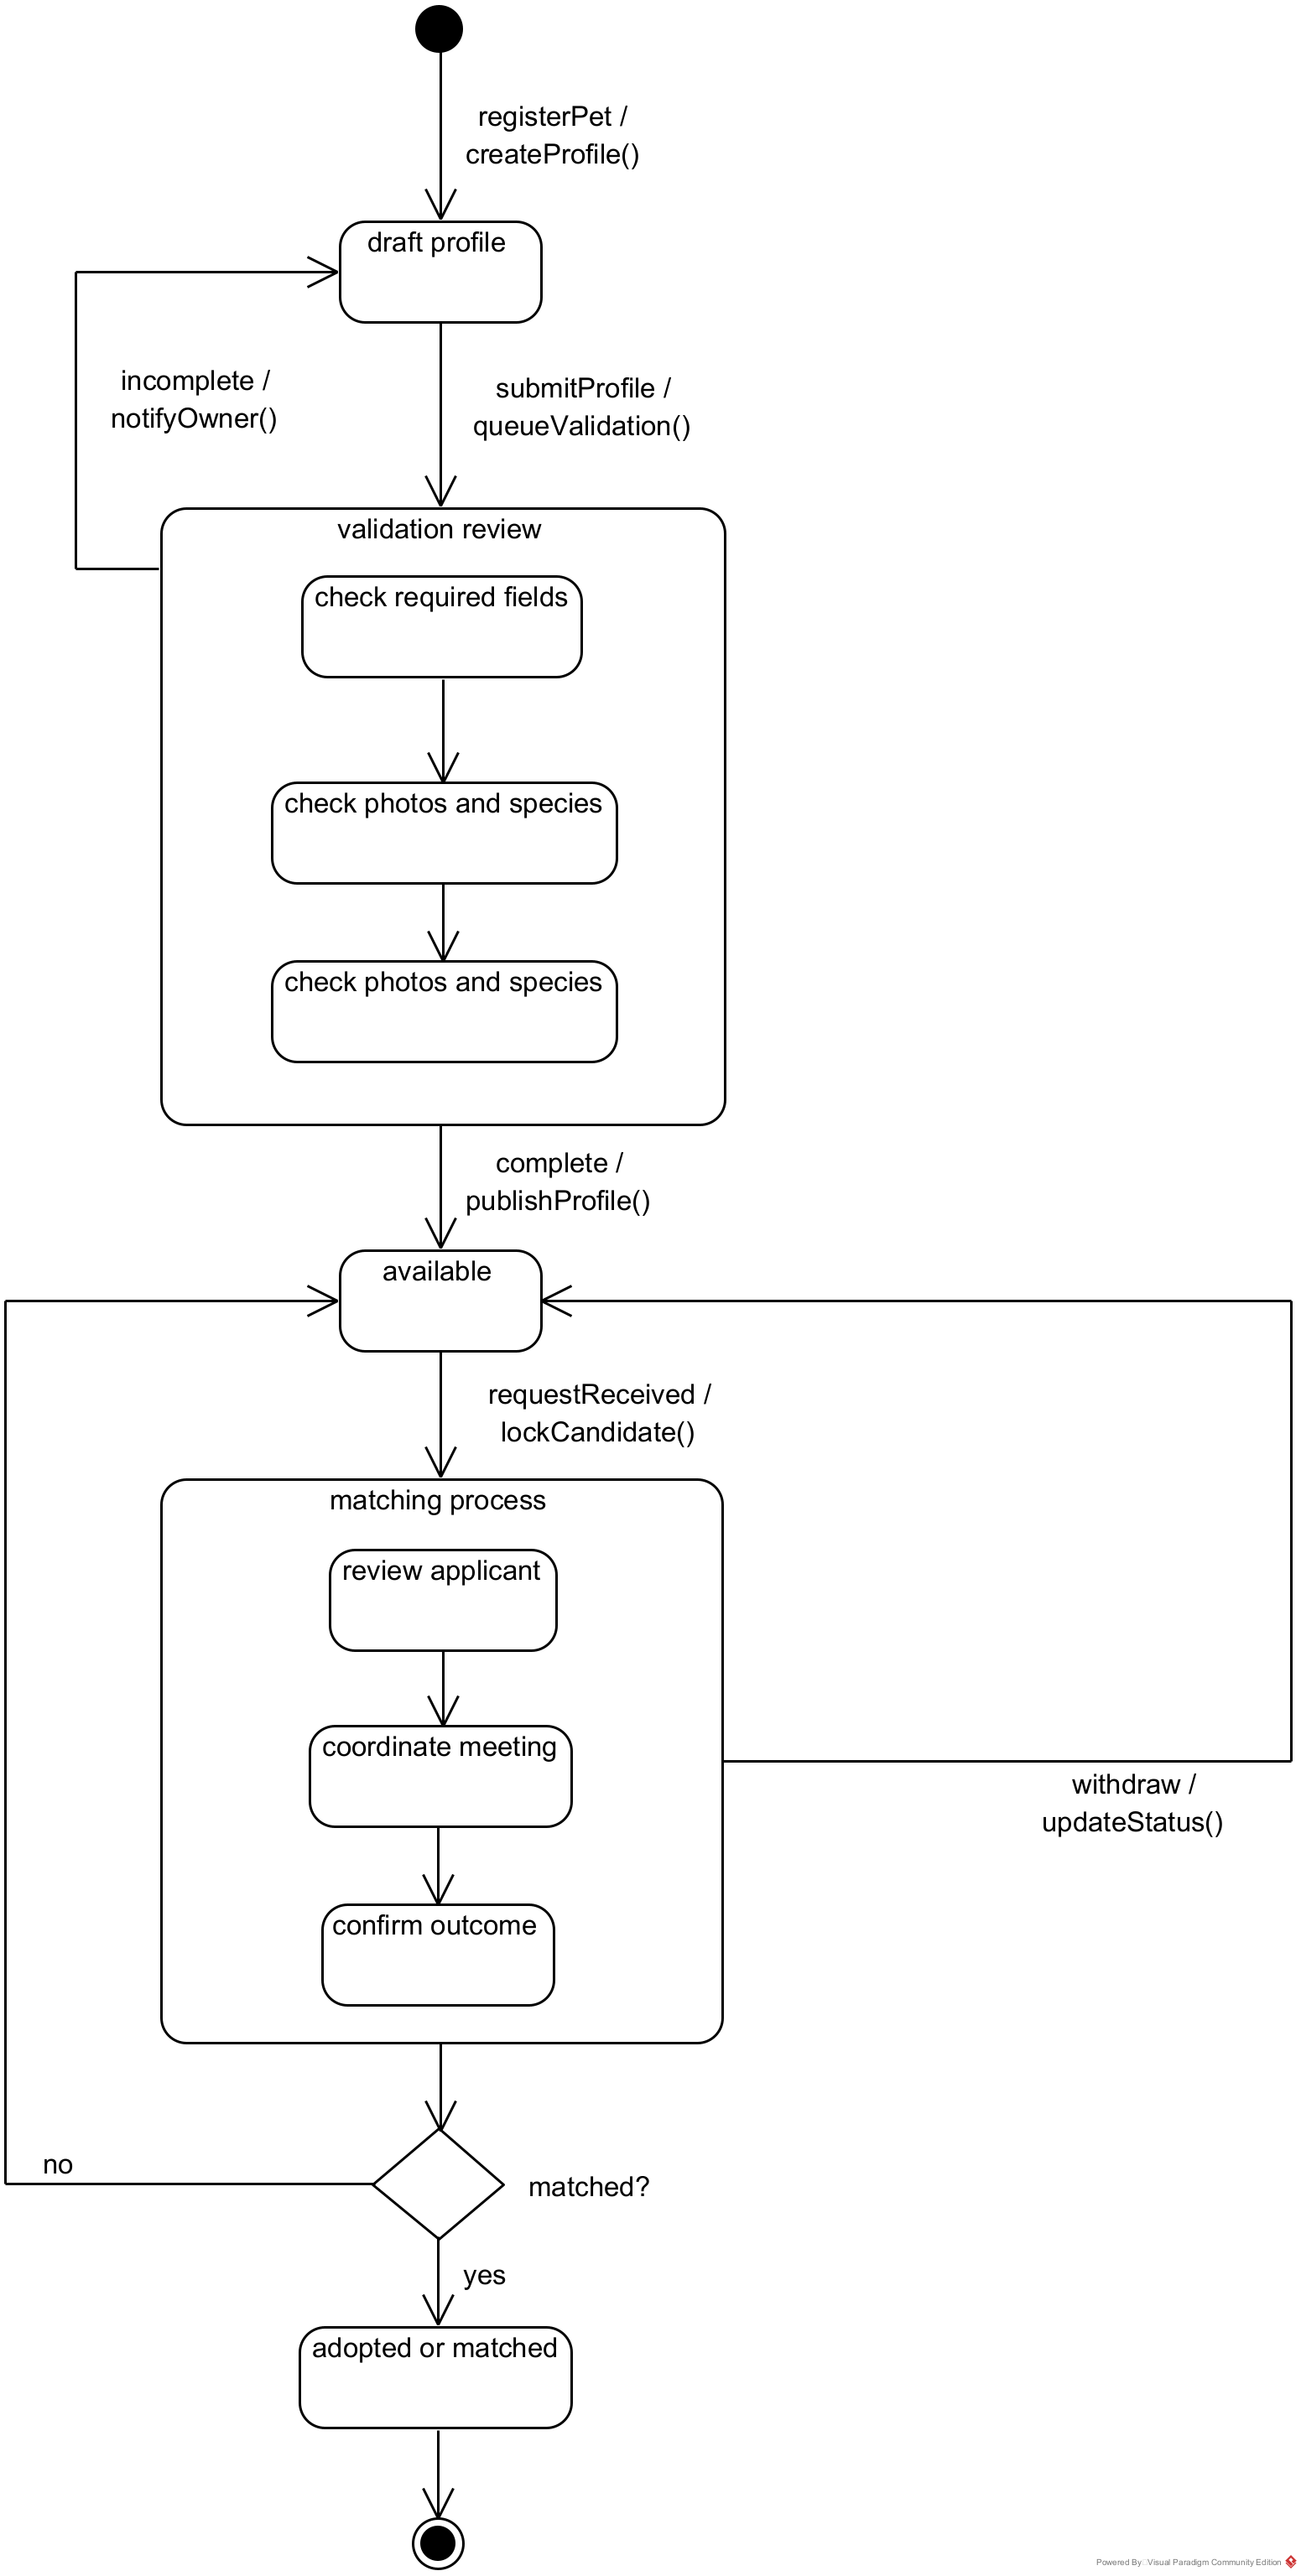
\includegraphics[width=0.50\textwidth]{figuras/DiagramaMaquinasEstado_PerfilMascota_MundiPets.png}
		\caption{Diagrama de estados del perfil de mascota.}
		\label{fig:est-mascota}
	\end{figure}
	
	\subsubsection{Estados de una solicitud de adopción o cruza}
	
	Esta máquina de estados formaliza el flujo por etapas exigido por RF-18 para
	las solicitudes de adopción, y el flujo más simple de aceptación o rechazo
	definido por RF-08 para las solicitudes de cruza. Una solicitud de adopción
	avanza secuencialmente por los estados \emph{Pendiente},
	\emph{EnEntrevista}, \emph{EnVisita}, \emph{EnPeriodoDePrueba} y
	\emph{Completada}, con la posibilidad de transitar a \emph{Rechazada} desde
	cualquiera de las etapas intermedias. Las transiciones están condicionadas
	por eventos generados por el propietario (aceptar, rechazar o avanzar de
	etapa) y quedan registradas para alimentar la consulta de historial de
	procesos definida en RF-15.
	
	\begin{figure}[H]
		\centering
		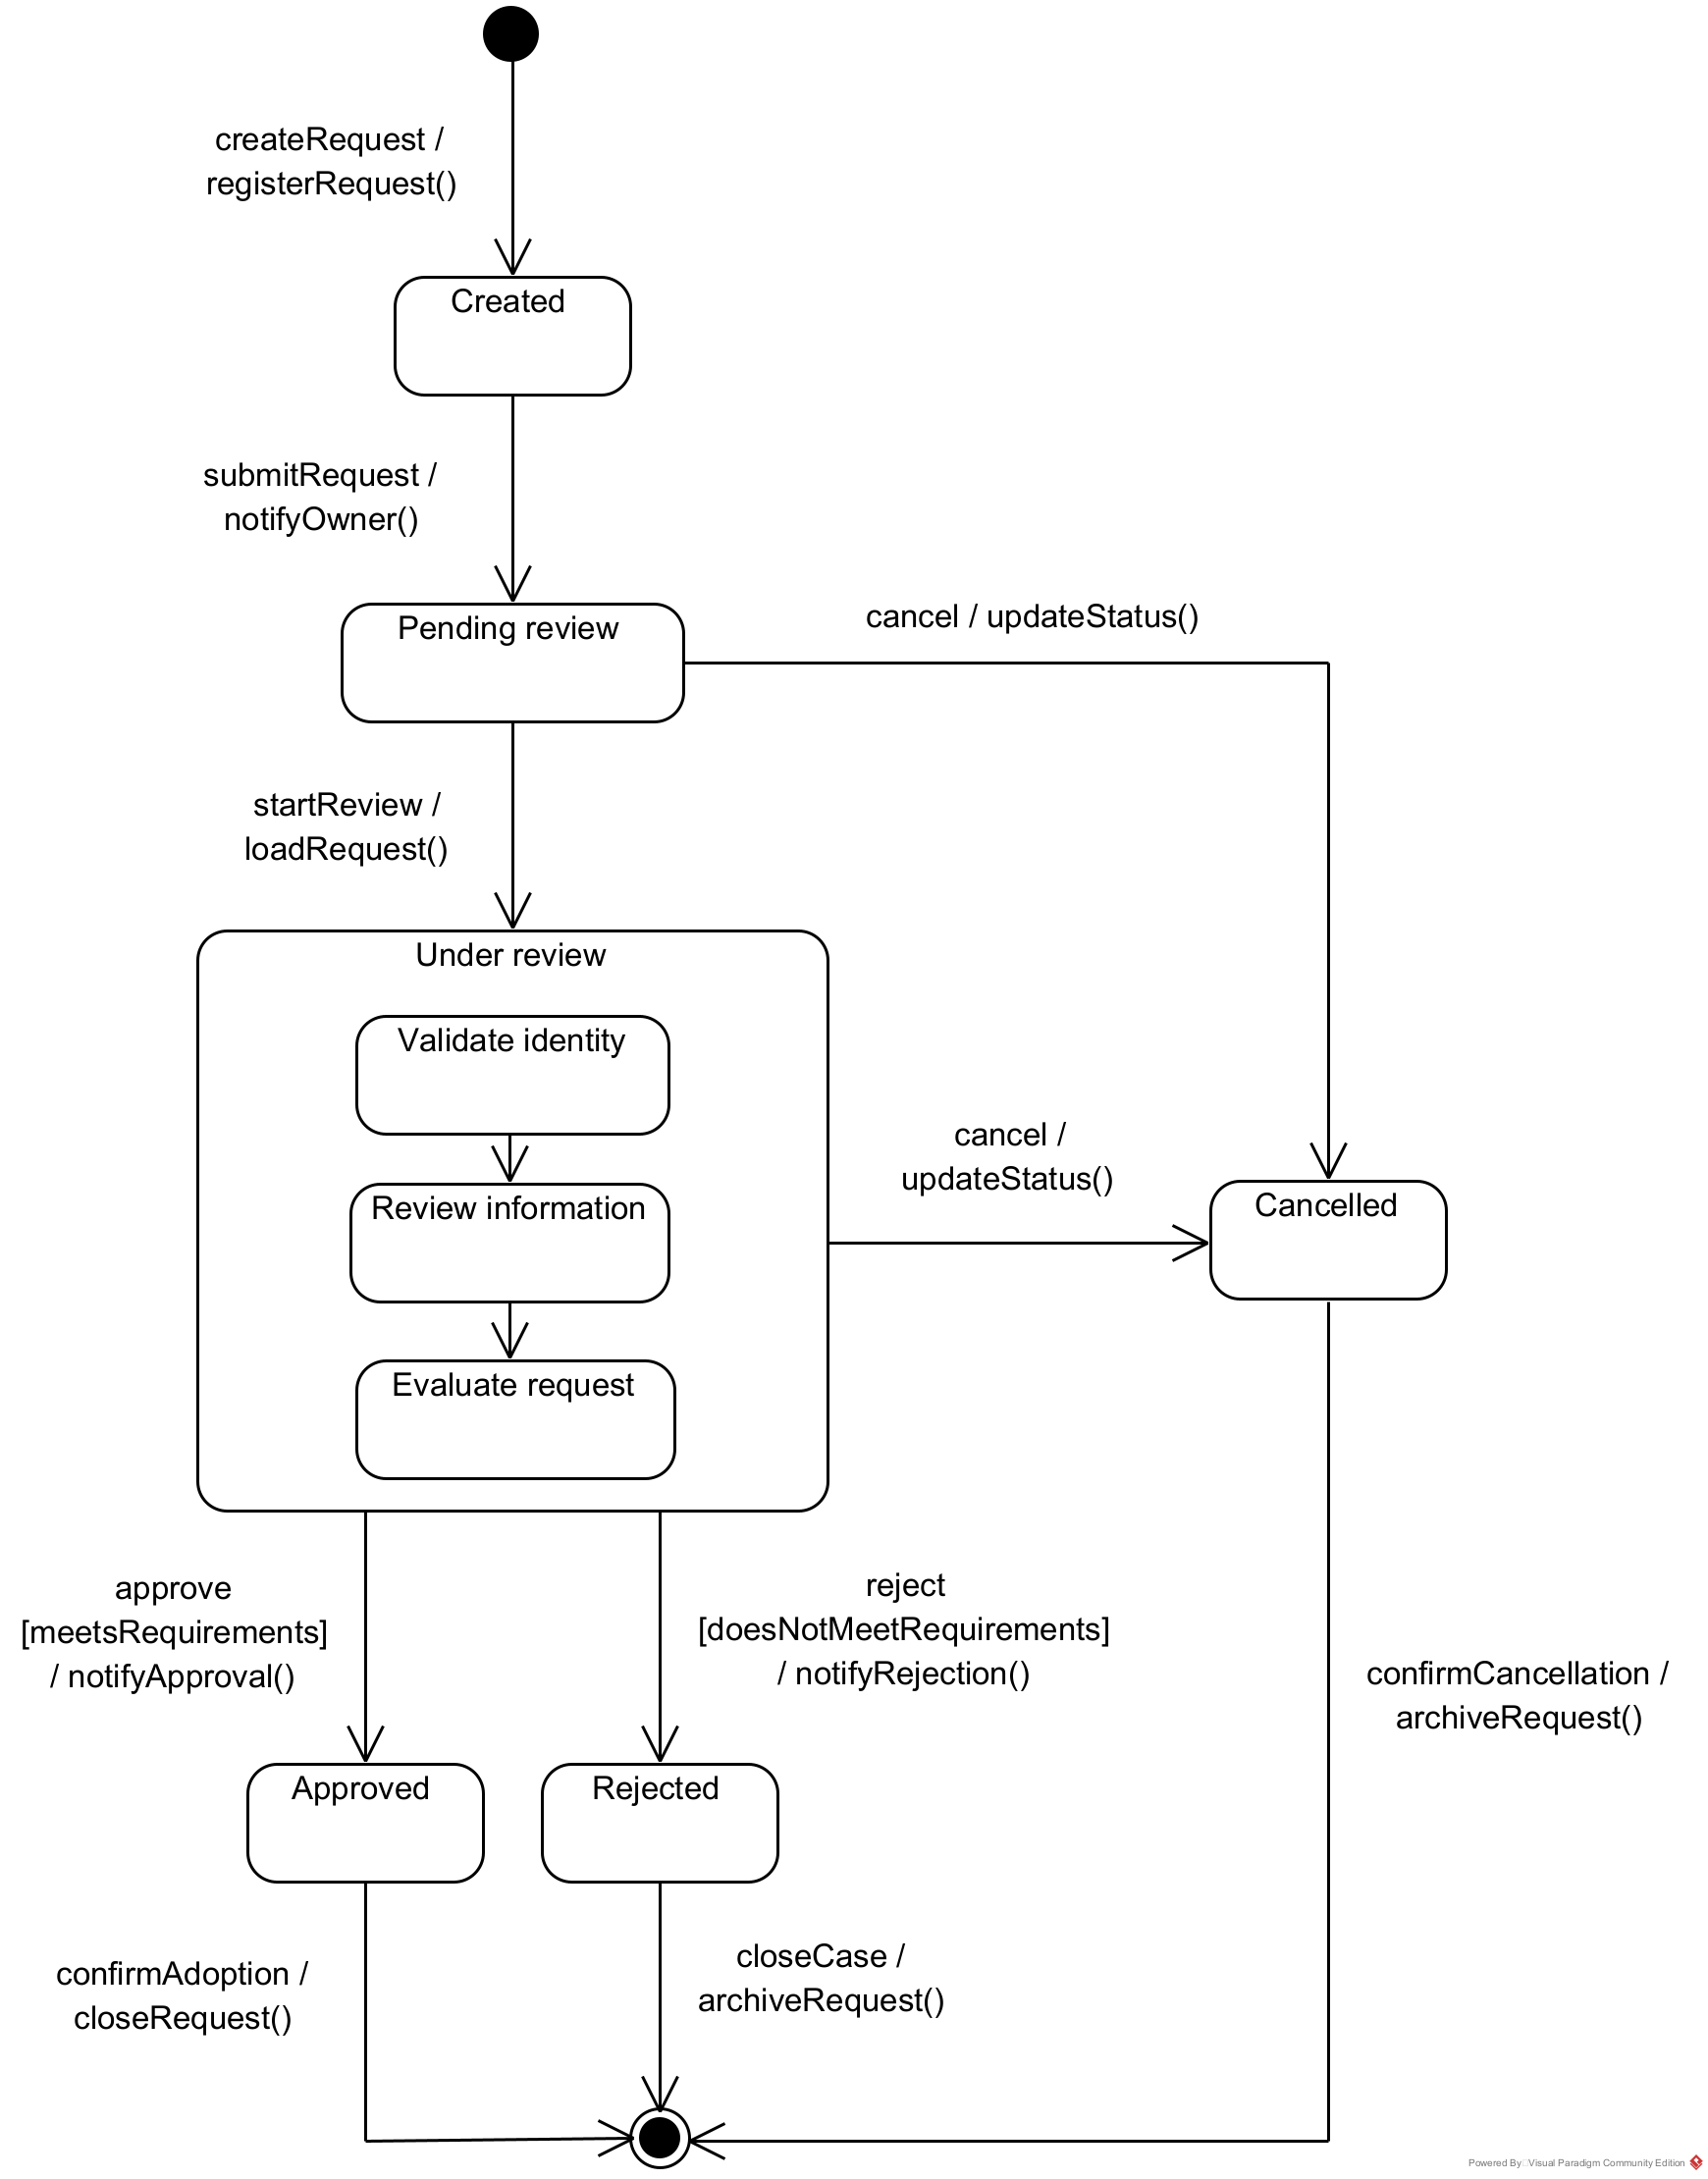
\includegraphics[width=0.79\textwidth]{figuras/DiagramaMaquinasEstado_Solicitudes_MundiPets.png}
		\caption{Diagrama de estados de una solicitud de adopción o cruza.}
		\label{fig:est-solicitud}
	\end{figure}
	
	\subsubsection{Estados de verificación de documentos médicos}
	
	La tercera máquina de estados corresponde al ciclo de vida de un documento
	médico cargado por el propietario (carnet de vacunación o certificado
	veterinario), desde su carga inicial en estado
	\emph{PendienteDeValidacion} hasta su resolución final en \emph{Validado} o
	\emph{Rechazado} por parte de una veterinaria autorizada, en cumplimiento de
	RD-03. El estado \emph{Rechazado} incluye obligatoriamente la observación
	técnica registrada por el profesional, y permite al propietario transitar
	nuevamente hacia \emph{PendienteDeValidacion} tras corregir o reemplazar el
	documento observado.
	
	\begin{figure}[H]
		\centering
		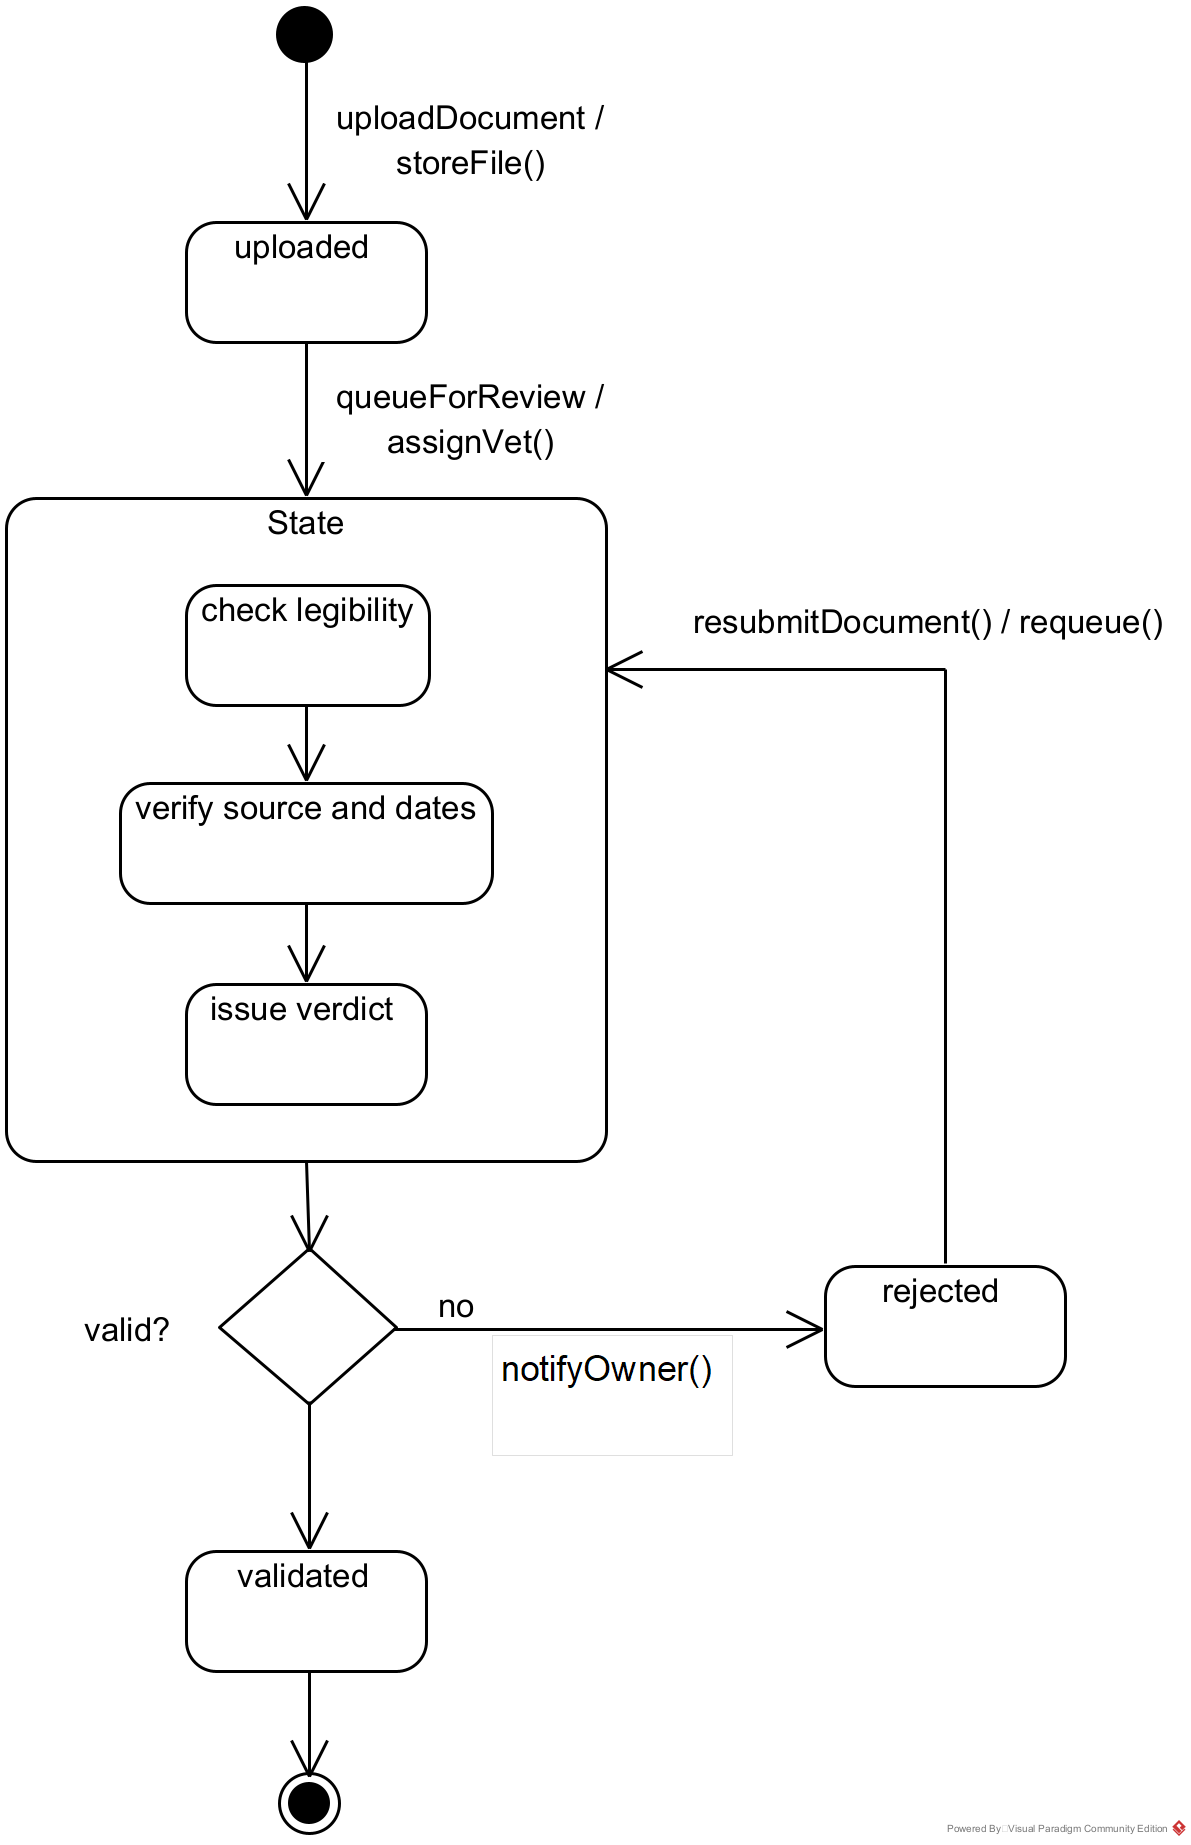
\includegraphics[width=0.65\textwidth]{figuras/DiagramaMaquinasEstado_VerificacionDocumentos_MundiPets.png}
		\caption{Diagrama de estados de verificación de documentos médicos.}
		\label{fig:est-documentos}
	\end{figure}
	
	% ------------------------------------------------------------
	\subsection{Diagrama de componentes}
	\label{sec:componentes}
	
	El diagrama de componentes traduce la restricción de arquitectura modular
	(RD-05) en una organización concreta de módulos de software con interfaces
	explícitas entre ellos. Se identifican cinco componentes principales:
	Gestión de Mascotas (RF-01, RF-02, RF-13, RF-16, RF-21), Adopción y Cruza
	(RF-05, RF-08, RF-18, RF-19, RF-20, RF-22), Mensajería (RF-07), Validación
	Médica (RF-09, RF-14, RF-24) y el componente de Inteligencia Artificial, que
	agrupa los tres subcomponentes de evaluación de compatibilidad (RF-06),
	validación de imágenes (RF-17) y moderación de mensajes.
	
	Las dependencias entre componentes se limitan a interfaces bien definidas:
	el componente de Adopción y Cruza depende de Gestión de Mascotas para
	consultar disponibilidad y antecedentes genéticos, pero no accede
	directamente a su modelo de datos interno; y el componente de Inteligencia
	Artificial expone una interfaz de evaluación que es consumida tanto por
	Adopción y Cruza como por Gestión de Mascotas, evitando que cada módulo
	implemente su propia lógica de IA. Este diseño sustenta directamente la
	métrica de mantenibilidad definida en RNF-10, según la cual una modificación
	en un componente no debería requerir cambios en más del 10\,\% de los
	archivos de otro módulo.
	
	\begin{figure}[H]
		\centering
		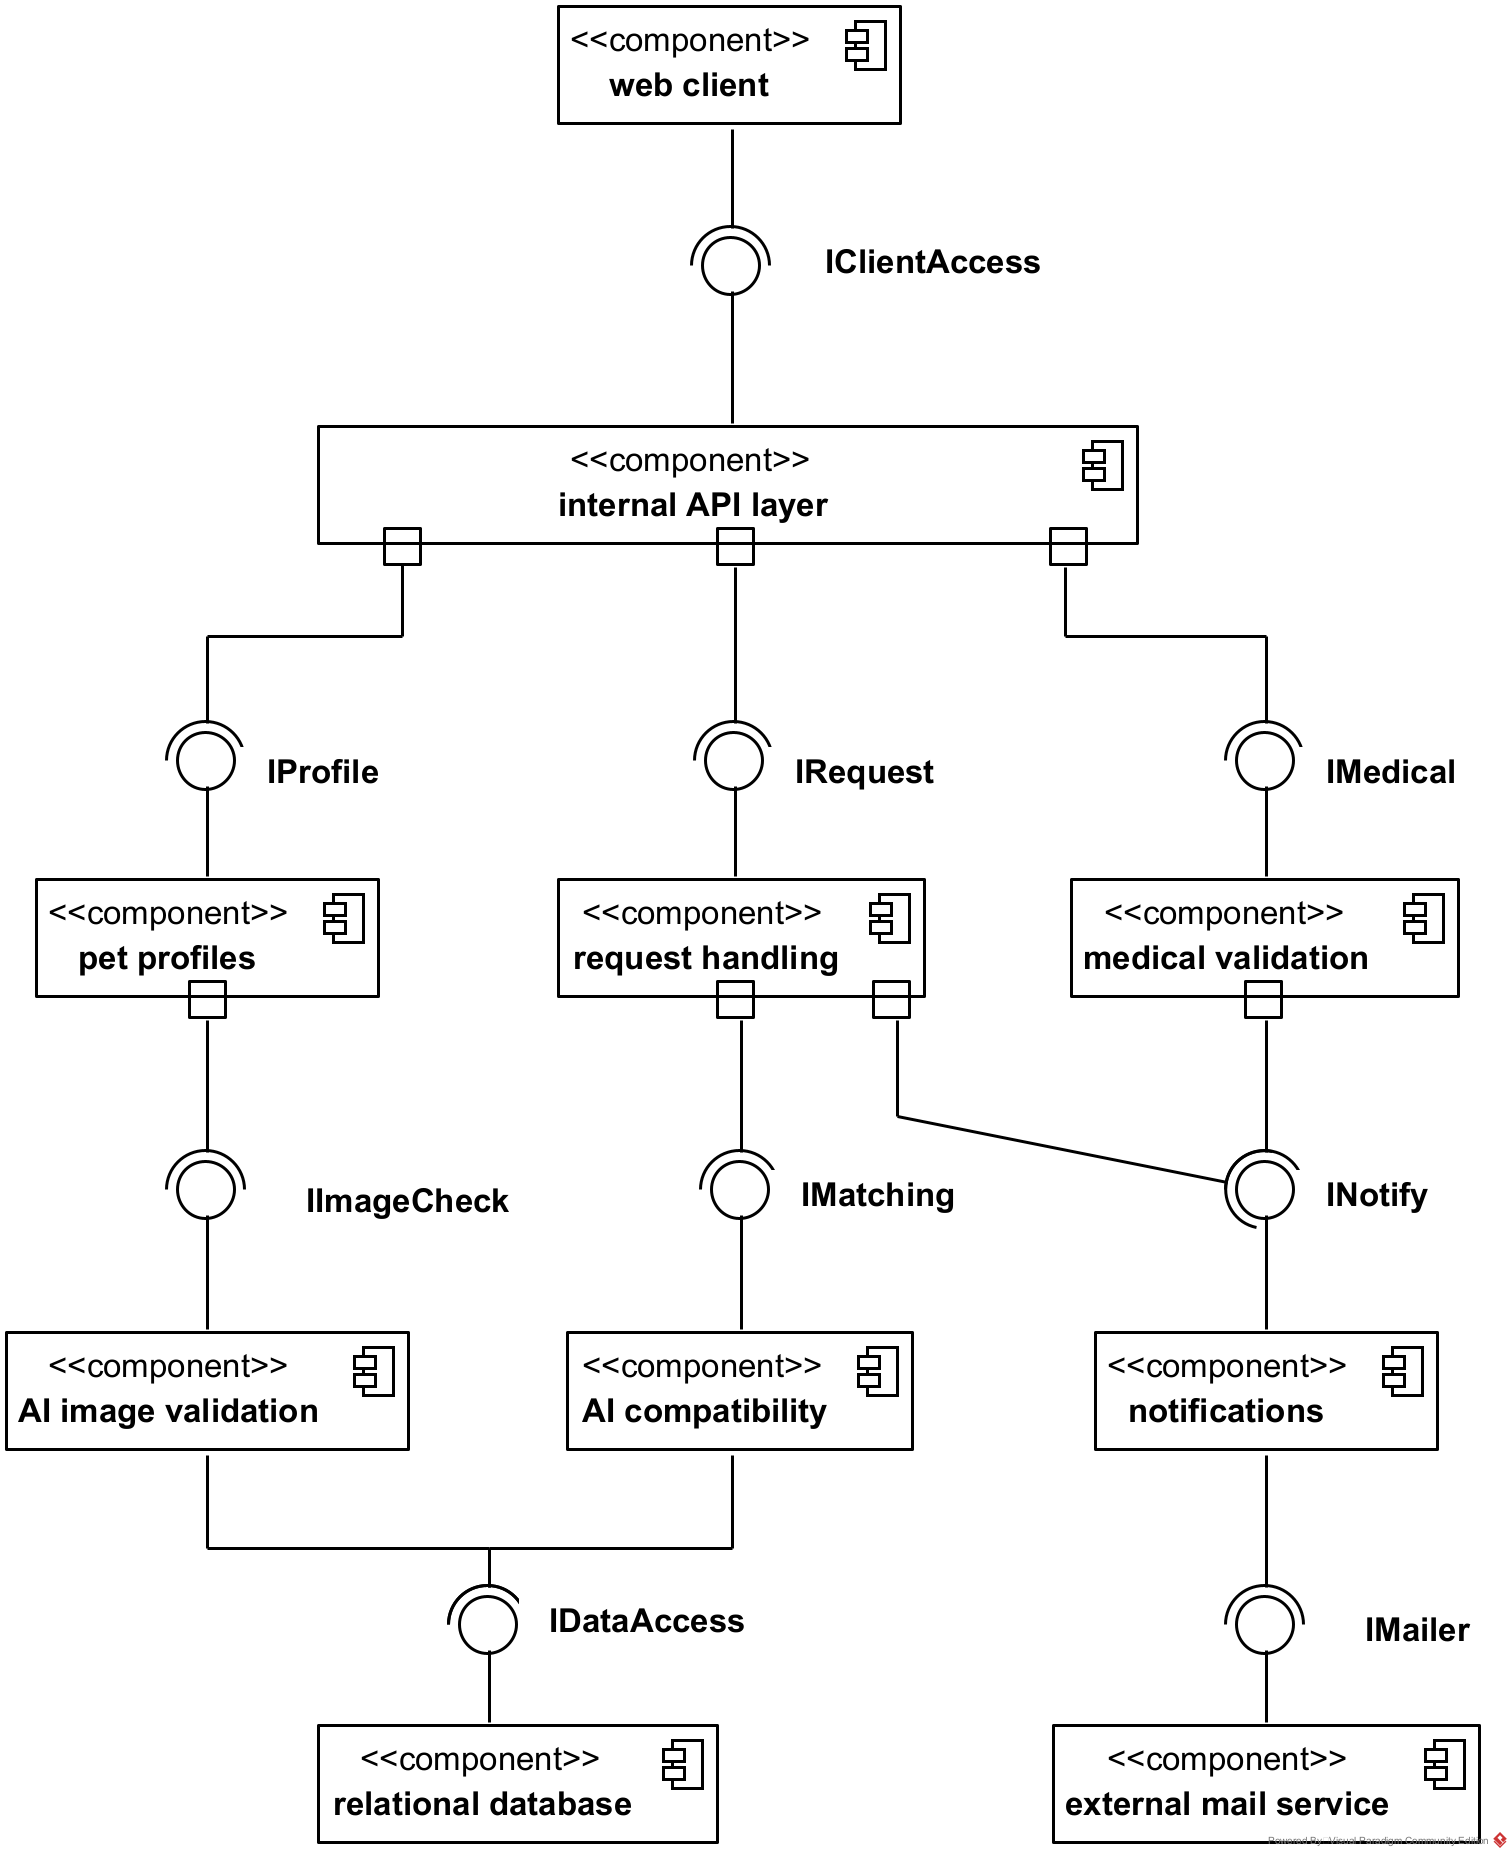
\includegraphics[width=0.75\textwidth]{figuras/DiagramaComponentes_MundiPets.png}
		\caption{Diagrama de componentes del sistema MundiPets.}
		\label{fig:componentes}
	\end{figure}
	
	% ------------------------------------------------------------
	\subsection{Diagrama de despliegue}
	\label{sec:despliegue}
	
	El diagrama de despliegue representa la distribución física de los
	componentes del sistema sobre la infraestructura de ejecución, en línea con
	el entorno operativo descrito en la Sección~\ref{sec:entorno}. Se modelan
	tres nodos principales: el dispositivo cliente (navegador web en computador,
	teléfono inteligente o tableta), el servidor de aplicaciones alojado en
	infraestructura en la nube, que ejecuta los componentes de Gestión de
	Mascotas, Adopción y Cruza, Mensajería y Validación Médica descritos en la
	Sección~\ref{sec:componentes}, y un servidor o servicio separado para el
	componente de Inteligencia Artificial, aislado por motivos de escalabilidad
	independiente del resto de la lógica de negocio.
	
	Un cuarto nodo representa el servidor de base de datos, que persiste tanto
	la información transaccional del sistema como los archivos multimedia
	(fotografías de mascotas y documentos veterinarios digitalizados). El
	diagrama incluye además la dependencia hacia el proveedor externo de
	mensajería (WhatsApp Business API) descrita en RD-08, necesaria para el
	envío de los recordatorios de controles preventivos definidos en RF-10. Esta
	separación de nodos permite que el servicio de inteligencia artificial
	escale de forma independiente al resto de la aplicación, en coherencia con
	la restricción de arquitectura modular (RD-05) y con la escalabilidad
	horizontal exigida por RNF-12.
	
	\begin{figure}[H]
		\centering
		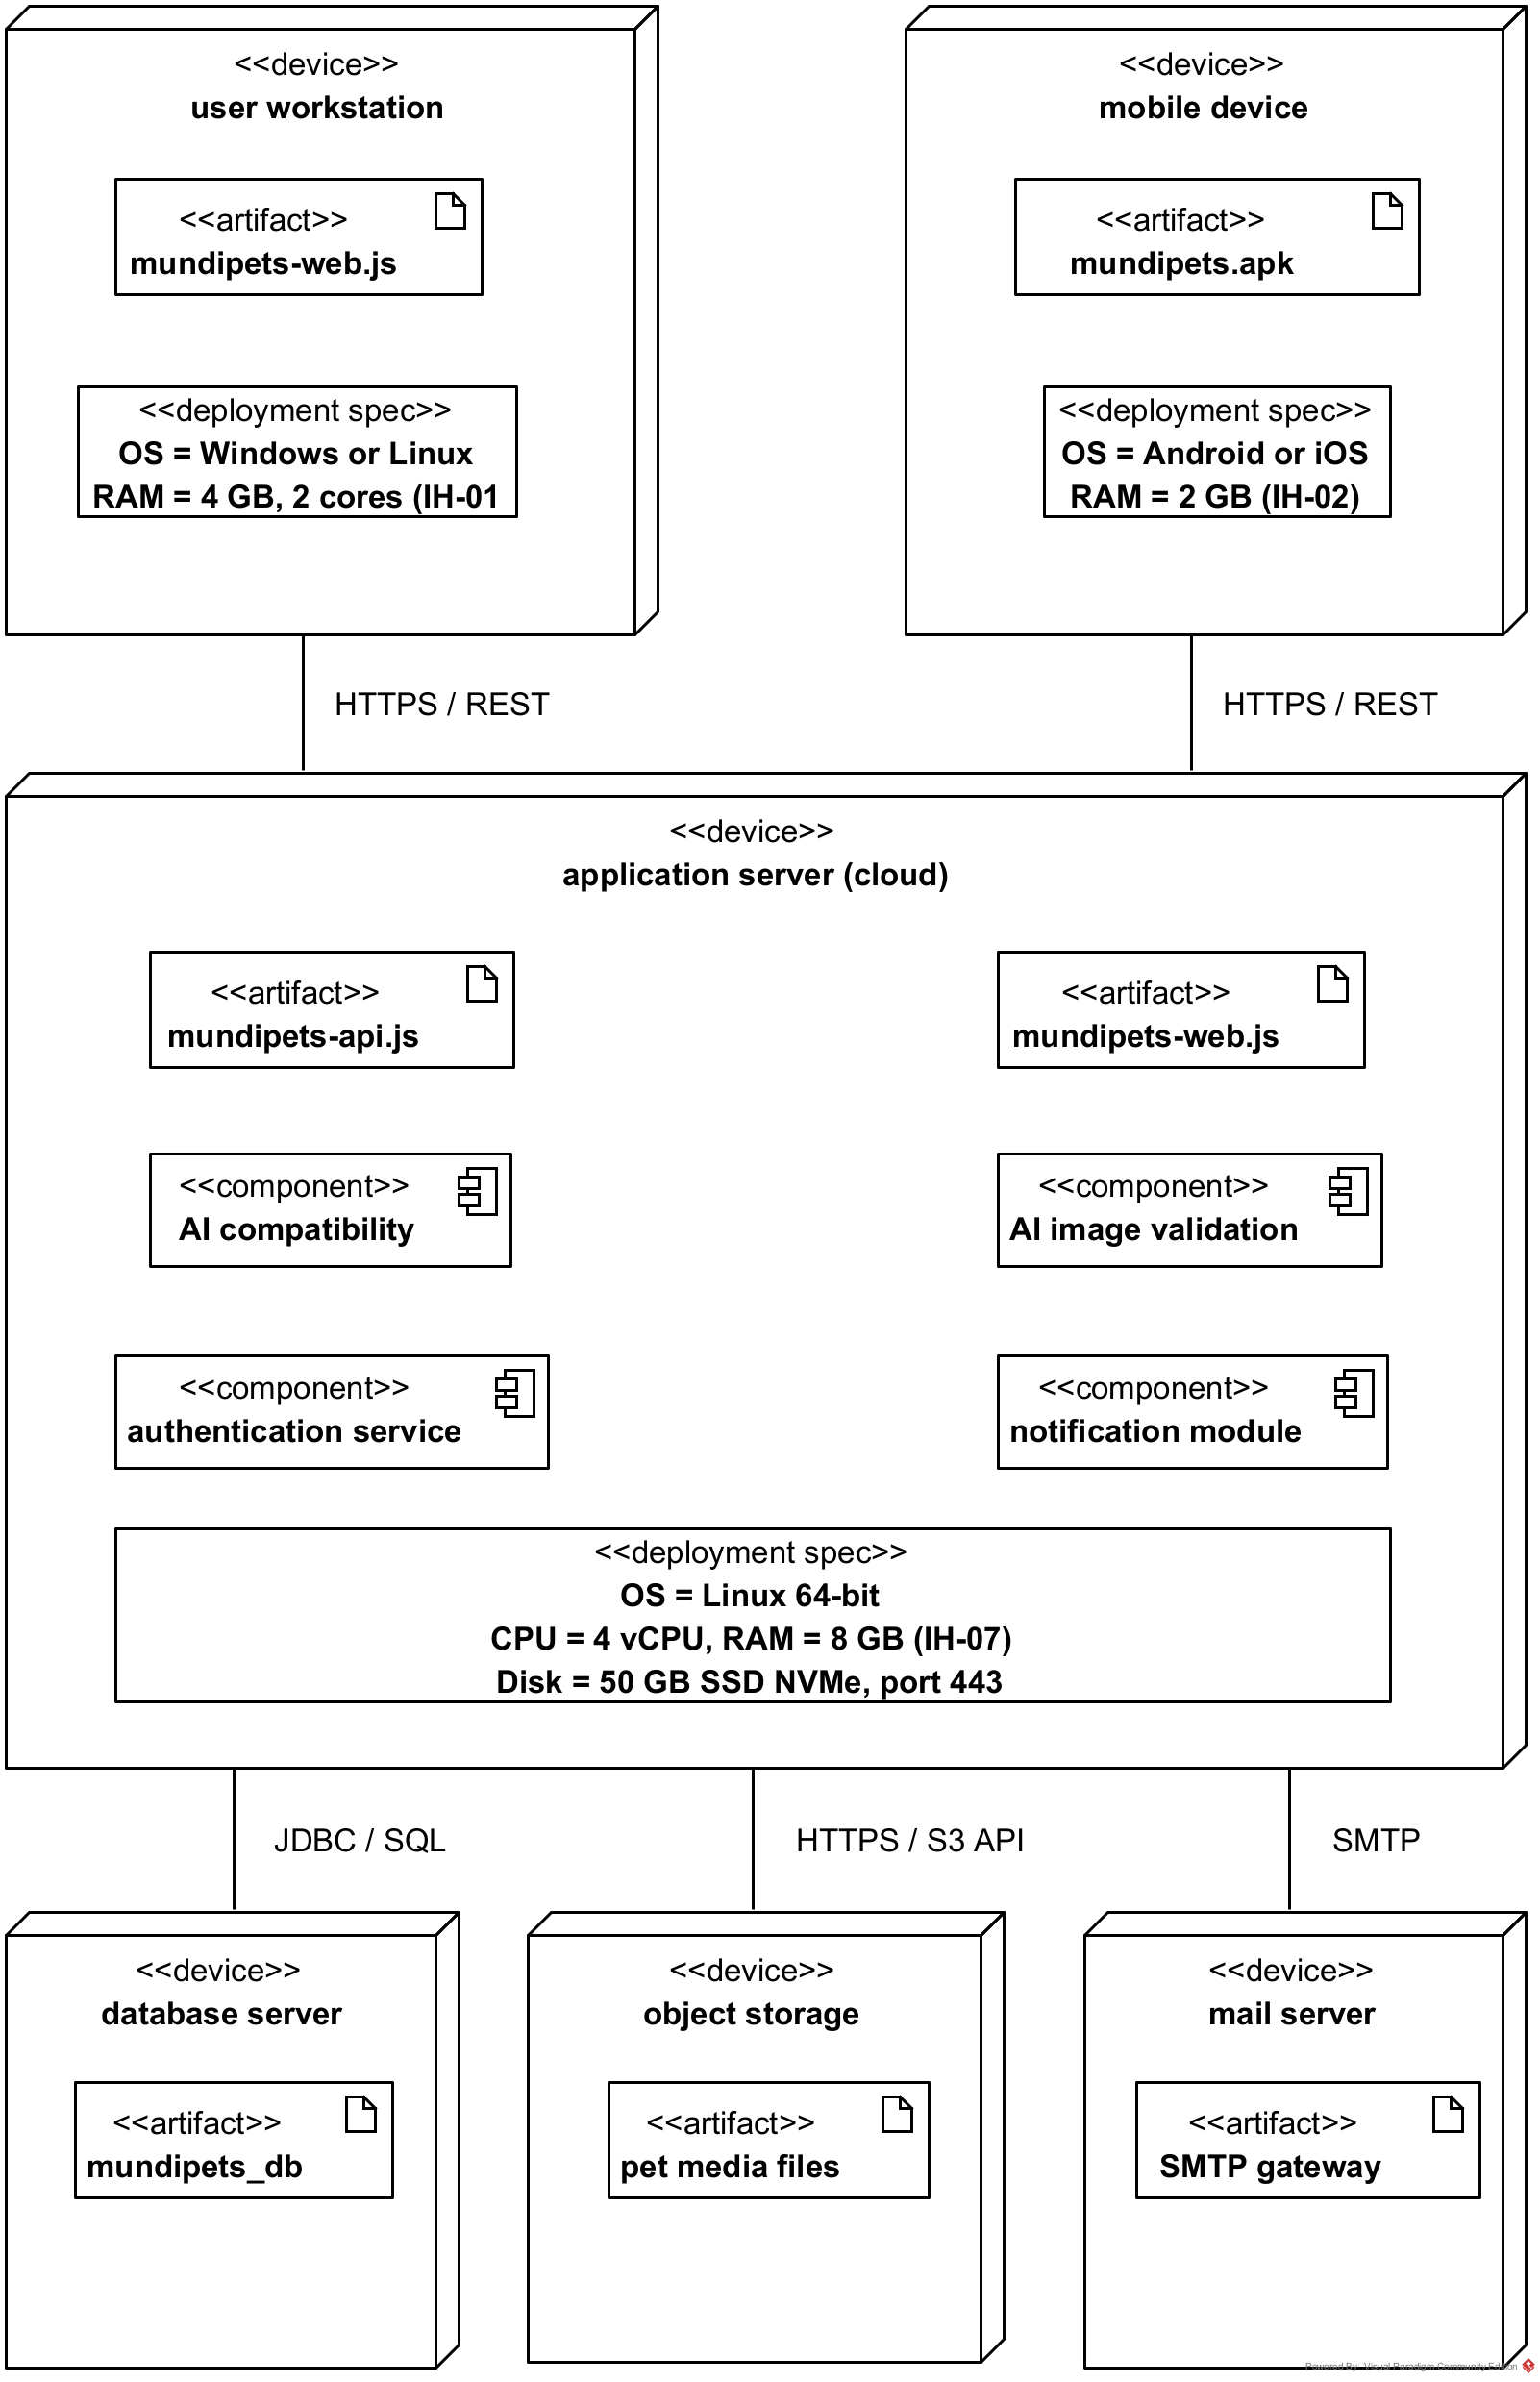
\includegraphics[width=0.65\textwidth]{figuras/DiagramaDespliegue_MundiPets.png}
		\caption{Diagrama de despliegue del sistema MundiPets.}
		\label{fig:despliegue}
	\end{figure}
	
	% ############################################################
	%        SECCION 5 -- PRIORIZACION Y TRAZABILIDAD EXTENDIDA
	% ############################################################
	\section{Priorización y trazabilidad extendida}
	\label{sec:priorizacion}
	
	\subsection{Clasificación de requisitos}
	\label{sec:clasificacion}
	
	En esta sección se presenta la clasificación general de los requisitos
	definidos para MundiPets, organizándolos según su identificador, nombre y
	tipo. La Tabla~\ref{tab:lista_requisitos_completa} recoge los 59 requisitos
	vigentes de la Entrega 3 (2A): 25 requisitos funcionales (RF-01 a RF-25),
	16 requisitos no funcionales (RNF-01 a RNF-16), 9 restricciones de diseño
	(RD-01 a RD-09) y 9 requisitos legales (RL-01 a RL-09), redactados en las
	Secciones~\ref{sec:rf}, \ref{sec:rnf}, \ref{sec:legales} y
	\ref{sec:restricciones}. Con ello se supera el piso mínimo de 25 RF y 15 RNF
	exigido por esta entrega.
	
	\begin{longtable}{@{}p{2.2cm} p{7.5cm} p{3.5cm}@{}}
		\caption{Clasificación de requisitos y restricciones (Entrega 2A).}
		\label{tab:lista_requisitos_completa} \\
		\hline
		\textbf{Identificador} & \textbf{Nombre del requisito} & \textbf{Clasificación} \\
		\hline
		\endfirsthead
		\multicolumn{3}{|l|}{\textit{(continuación)}} \\
		\hline
		\textbf{Identificador} & \textbf{Nombre del requisito} & \textbf{Clasificación} \\
		\hline
		\endhead
		\hline
		\endfoot
		RF-01 & Registrar mascota & Requisito funcional \\
		\hline
		RF-02 & Gestionar historial médico de la mascota & Requisito funcional \\
		\hline
		RF-03 & Consultar perfil completo de una mascota & Requisito funcional \\
		\hline
		RF-04 & Buscar y filtrar mascotas & Requisito funcional \\
		\hline
		RF-05 & Gestionar solicitudes de adopción & Requisito funcional \\
		\hline
		RF-06 & Evaluar compatibilidad entre mascotas para cruza & Requisito funcional \\
		\hline
		RF-07 & Sistema de mensajería entre usuarios & Requisito funcional \\
		\hline
		RF-08 & Gestionar solicitudes de cruza & Requisito funcional \\
		\hline
		RF-09 & Validar la información médica de una mascota & Requisito funcional \\
		\hline
		RF-10 & Gestionar recordatorios de controles preventivos & Requisito funcional \\
		\hline
		RF-11 & Administrar la privacidad de la información & Requisito funcional \\
		\hline
		RF-12 & Verificar la identidad de los usuarios & Requisito funcional \\
		\hline
		RF-13 & Registrar publicaciones de mascotas & Requisito funcional \\
		\hline
		RF-14 & Gestionar carnet de vacunación & Requisito funcional \\
		\hline
		RF-15 & Consultar el historial de procesos de adopción y cruza & Requisito funcional \\
		\hline
		RF-16 & Gestionar antecedentes genéticos y parentesco de la mascota & Requisito funcional \\
		\hline
		RF-17 & Validar imágenes & Requisito funcional \\
		\hline
		RF-18 & Gestionar el flujo de solicitud de adopción por etapas & Requisito funcional \\
		\hline
		RF-19 & Validar certificados veterinarios antes de habilitar la cruza & Requisito funcional \\
		\hline
		RF-20 & Coordinar encuentros de socialización supervisados & Requisito funcional \\
		\hline
		RF-21 & Registrar el identificador de microchip de la mascota & Requisito funcional \\
		\hline
		RF-22 & Dar seguimiento post-adopción & Requisito funcional \\
		\hline
		RF-23 & Emitir alertas de riesgo sanitario o físico en interacciones y cruces & Requisito funcional \\
		\hline
		RF-24 & Registrar trazabilidad de cepa, lote y aplicador de cada vacuna & Requisito funcional \\
		\hline
		RF-25 & Publicar aviso de mascota extraviada & Requisito funcional \\
		\hline
		RNF-01 & Protección de la información de propietarios y mascotas & Requisito no funcional \\
		\hline
		RNF-02 & Disponibilidad del sistema & Requisito no funcional \\
		\hline
		RNF-03 & Tiempo de respuesta del sistema & Requisito no funcional \\
		\hline
		RNF-04 & Facilidad de uso de la plataforma & Requisito no funcional \\
		\hline
		RNF-05 & Integridad de la información médica & Requisito no funcional \\
		\hline
		RNF-06 & Exactitud del componente de inteligencia artificial & Requisito no funcional \\
		\hline
		RNF-07 & Precisión en la validación de imágenes & Requisito no funcional \\
		\hline
		RNF-08 & Actualización de la información registrada & Requisito no funcional \\
		\hline
		RNF-09 & Interoperabilidad de notificaciones con canales externos & Requisito no funcional \\
		\hline
		RNF-10 & Facilidad de mantenimiento del código & Requisito no funcional \\
		\hline
		RNF-11 & Portabilidad entre navegadores y dispositivos & Requisito no funcional \\
		\hline
		RNF-12 & Escalabilidad ante crecimiento de usuarios & Requisito no funcional \\
		\hline
		RNF-13 & Explicabilidad de la recomendación de compatibilidad para cruza & Requisito no funcional \\
		\hline
		RNF-14 & Explicabilidad del rechazo o aceptación de imágenes & Requisito no funcional \\
		\hline
		RNF-15 & Explicabilidad de la moderación de mensajes & Requisito no funcional \\
		\hline
		RNF-16 & Confidencialidad de datos de ubicación y contacto & Requisito no funcional \\
		\hline
		RD-01 & Integración de componentes de inteligencia artificial & Restricción de diseño \\
		\hline
		RD-02 & Acceso basado en roles & Restricción de diseño \\
		\hline
		RD-03 & Validación profesional de la información médica & Restricción de diseño \\
		\hline
		RD-04 & Protección de datos personales & Restricción de diseño \\
		\hline
		RD-05 & Arquitectura modular del sistema & Restricción de diseño \\
		\hline
		RD-06 & Mecanismo de eliminación de cuenta y datos personales & Restricción de diseño \\
		\hline
		RD-07 & Protocolo de notificación de vulneraciones de seguridad & Restricción de diseño \\
		\hline
		RD-08 & Dependencia de servicios externos de mensajería & Restricción de diseño \\
		\hline
		RD-09 & Anonimización de evidencias de campo para publicación abierta & Restricción de diseño \\
		\hline
		RL-01 & Consentimiento libre, específico, informado e inequívoco & Requisito legal \\
		\hline
		RL-02 & Información de finalidad y derecho de acceso & Requisito legal \\
		\hline
		RL-03 & Derecho de rectificación y actualización & Requisito legal \\
		\hline
		RL-04 & Derecho de supresión de datos personales & Requisito legal \\
		\hline
		RL-05 & Minimización y seguridad de los datos & Requisito legal \\
		\hline
		RL-06 & Derecho a explicación de decisiones automatizadas & Requisito legal \\
		\hline
		RL-07 & Confidencialidad reforzada de datos sensibles y de salud & Requisito legal \\
		\hline
		RL-08 & Protección de datos desde el diseño y por defecto & Requisito legal \\
		\hline
		RL-09 & Notificación de vulneraciones de seguridad & Requisito legal \\
	\end{longtable}
	
	\newpage
	
	\subsection{Priorización MoSCoW}
	\label{sec:moscow}
	
	La Tabla~\ref{tab:priorizacion_moscow_parcial} presenta la priorización
	MoSCoW extendida de los 59 requisitos vigentes del proyecto, actualizando y
	ampliando la clasificación heredada de la Entrega 2 (1B) con los
	identificadores incorporados en esta entrega (RF-18 a RF-25, RNF-09 a
	RNF-16, RD-06 a RD-09 y RL-01 a RL-09). La misma priorización, junto con su
	clasificación Kano y su valor WSJF, se consolida en el
	\textbf{\hyperref[tab:priorizacion_moscow_completa]{Apéndice C --- Priorización
			MoSCoW, Kano y WSJF (detalle)}}.
	
	\begin{longtable}{@{}p{1.6cm} p{4.8cm} p{1.6cm} p{5.2cm}@{}}
		\caption{Priorización MoSCoW extendida (Entrega 2A).}
		\label{tab:priorizacion_moscow_parcial} \\
		\hline
		\textbf{ID} & \textbf{Requisito} & \textbf{Prioridad} & \textbf{Justificación} \\
		\hline
		\endfirsthead
		\multicolumn{4}{|l|}{\textit{(continuación)}} \\
		\hline
		\textbf{ID} & \textbf{Requisito} & \textbf{Prioridad} & \textbf{Justificación} \\
		\hline
		\endhead
		\hline
		\endfoot
		RF-01 & Registrar mascota & Must & Es el pilar del sistema; sin este RF no puede existir ningún perfil de mascota ni proceso posterior. \\
		\hline
		RF-02 & Gestionar historial médico & Must & Crítico para la salud animal y para RL-03 (rectificación de datos médicos). \\
		\hline
		RF-03 & Consultar perfil completo & Must & Fundamental para que adoptantes e interesados en cruza tomen decisiones informadas; sustenta RL-02. \\
		\hline
		RF-04 & Buscar y filtrar mascotas & Should & Mejora la usabilidad, pero el sistema puede operar inicialmente con listas generales. \\
		\hline
		RF-05 & Gestionar solicitudes de adopción & Must & Núcleo del modelo operativo de la plataforma. \\
		\hline
		RF-06 & Evaluar compatibilidad para cruza & Must & Requisito diferenciador que usa IA; motivó RD-01 y exige la explicabilidad de RL-06. \\
		\hline
		RF-07 & Sistema de mensajería & Could & Deseable para coordinar procesos, pero el contacto inicial puede derivarse a canales externos si hay limitaciones de tiempo. \\
		\hline
		RF-08 & Gestionar solicitudes de cruza & Must & Operación central del modelo de negocio junto a RF-05. \\
		\hline
		RF-09 & Validar información médica & Must & Imprescindible para la confiabilidad clínica del sistema. \\
		\hline
		RF-10 & Recordatorios de controles preventivos & Should & Aporta valor de bienestar animal, pero no bloquea el flujo principal de adopciones. \\
		\hline
		RF-11 & Administrar privacidad & Must & Mandatorio por RL-02 y RL-05; es el RF más citado en las entrevistas (9 EV). \\
		\hline
		RF-12 & Verificar identidad de usuarios & Must & Indispensable para evitar fraude; sustenta el consentimiento de RL-01. \\
		\hline
		RF-13 & Registrar publicaciones & Must & Necesario para que un propietario active la disponibilidad de su mascota. \\
		\hline
		RF-14 & Gestionar carnet de vacunación & Must & Crítico para la trazabilidad sanitaria; sustenta RL-03. \\
		\hline
		RF-15 & Consultar historial de procesos & Could & Aporta trazabilidad al usuario, pero no es indispensable para completar una adopción o cruza. \\
		\hline
		RF-16 & Antecedentes genéticos y parentesco & Must & Necesario para que RF-06 pueda evaluar compatibilidad de forma responsable. \\
		\hline
		RF-17 & Validar imágenes con IA & Should & Refuerza la seguridad del contenido, pero el sistema puede operar con moderación manual inicial. \\
		\hline
		RF-18 & Flujo de adopción por etapas & Must & Formaliza el proceso de adopción responsable identificado en la segunda ronda de campo (EV-11, EV-16). \\
		\hline
		RF-19 & Validar certificados veterinarios antes de cruza & Should & Refuerza la confiabilidad de RF-06, pero no bloquea su funcionamiento básico. \\
		\hline
		RF-20 & Encuentros de socialización supervisados & Could & Valor deseable de bienestar animal, mencionado por un solo participante (EV-13). \\
		\hline
		RF-21 & Registrar identificador de microchip & Should & Aporta trazabilidad complementaria al carnet de vacunación. \\
		\hline
		RF-22 & Seguimiento post-adopción & Must & Cierra el ciclo de responsabilidad de RF-18, exigido por participantes de la segunda ronda. \\
		\hline
		RF-23 & Alertas de riesgo sanitario o físico & Must & Mitiga un riesgo real de seguridad y salud animal detectado en varias entrevistas (EV-09, EV-12, EV-15, EV-18). \\
		\hline
		RF-24 & Trazabilidad de cepa, lote y aplicador & Should & Complementa RF-14 con datos adicionales de trazabilidad, no bloqueante. \\
		\hline
		RF-25 & Aviso de mascota extraviada & Could & Funcionalidad de valor social, pero fuera del núcleo de adopción/cruza del sistema. \\
		\hline
		RNF-01 & Protección de información de propietarios y mascotas & Must & Requisito estricto de seguridad; sustenta RL-05 y RL-07. \\
		\hline
		RNF-02 & Disponibilidad del sistema & Must & Crítico para la operatividad continua de la plataforma. \\
		\hline
		RNF-03 & Tiempo de respuesta del sistema & Should & Mejora la experiencia, pero el sistema es funcional con tiempos mayores en una primera versión. \\
		\hline
		RNF-04 & Facilidad de uso de la plataforma & Should & Relevante para adopción del producto, pero no bloquea sus funciones. \\
		\hline
		RNF-05 & Integridad de la información médica & Must & Evita modificaciones no autorizadas del historial clínico; sustenta RL-07. \\
		\hline
		RNF-06 & Exactitud del componente de IA & Must & Sin una precisión mínima, RF-06 pierde su valor diferenciador. \\
		\hline
		RNF-07 & Precisión en validación de imágenes & Should & Mejora la calidad del contenido, pero RF-17 puede operar con una tasa de error inicial mayor. \\
		\hline
		RNF-08 & Actualización de la información registrada & Should & Mejora la confianza del usuario, no bloquea el flujo principal. \\
		\hline
		RNF-09 & Interoperabilidad de notificaciones & Should & Aporta valor (recordatorios por WhatsApp), pero el sistema opera sin ella mediante notificación interna. \\
		\hline
		RNF-10 & Facilidad de mantenimiento del código & Should & Importante para sostenibilidad técnica, pero no bloquea la operación funcional del MVP. \\
		\hline
		RNF-11 & Portabilidad entre navegadores & Should & Necesaria para alcance de usuarios, pero el sistema puede operar inicialmente en un navegador principal. \\
		\hline
		RNF-12 & Escalabilidad ante crecimiento de usuarios & Could & Deseable a mediano plazo; no crítica mientras la base de usuarios sea reducida. \\
		\hline
		RNF-13 & Explicabilidad de compatibilidad para cruza & Must & Exigido por el derecho legal a explicación (RL-06) sobre decisiones automatizadas del RF-06. \\
		\hline
		RNF-14 & Explicabilidad de rechazo de imágenes & Should & Mejora la confianza del usuario, pero el sistema puede operar con un mensaje de rechazo genérico inicialmente. \\
		\hline
		RNF-15 & Explicabilidad de moderación de mensajes & Should & Igual que RNF-14: deseable para confianza, no bloqueante. \\
		\hline
		RNF-16 & Confidencialidad de ubicación y contacto & Must & Obligación legal directa (RL-05, principio de minimización). \\
		\hline
		RD-01 & Integración de componentes de IA & Must & Restricción ineludible: arquitectura del principal valor agregado de MundiPets. \\
		\hline
		RD-02 & Acceso basado en roles & Must & Mandatorio para diferenciar permisos de propietarios, veterinarias y administradores; sustenta RL-05 y RL-08. \\
		\hline
		RD-03 & Validación profesional de la información médica & Must & Exigido por los veterinarios entrevistados para garantizar confiabilidad clínica. \\
		\hline
		RD-04 & Protección de datos personales & Must & Implementa directamente RL-05, RL-07 y RL-08. \\
		\hline
		RD-05 & Arquitectura modular del sistema & Must & Facilita mantenimiento e incorporación de nuevas funcionalidades; sustenta RNF-10. \\
		\hline
		RD-06 & Eliminación de cuenta y datos personales & Must & Obligación legal ineludible (RL-04, derecho de supresión); sin este mecanismo el sistema incumple la LOPDP. \\
		\hline
		RD-07 & Protocolo de notificación de vulneraciones & Must & Exigido por RL-09 con plazos legales estrictos (5 y 3 días). \\
		\hline
		RD-08 & Dependencia de servicios externos de mensajería & Should & Aporta valor (RF-10) pero requiere un canal de respaldo ante caídas del proveedor. \\
		\hline
		RD-09 & Anonimización de evidencias para publicación abierta & Must & Exigido por los Art. 30-32 LOPDP para el uso de datos de investigación en el paquete FAIR. \\
		\hline
		RL-01 & Consentimiento libre, específico, informado e inequívoco & Must & Toda obligación legal es no negociable: su incumplimiento expone al proyecto a responsabilidad legal. \\
		\hline
		RL-02 & Información de finalidad y derecho de acceso & Must & Ídem: obligación legal directa (Art. 12-13 LOPDP). \\
		\hline
		RL-03 & Derecho de rectificación y actualización & Must & Ídem: obligación legal directa (Art. 14 LOPDP). \\
		\hline
		RL-04 & Derecho de supresión de datos personales & Must & Ídem: obligación legal directa (Art. 15 LOPDP). \\
		\hline
		RL-05 & Minimización y seguridad de los datos & Must & Ídem: obligación legal directa (Art. 10 LOPDP). \\
		\hline
		RL-06 & Derecho a explicación de decisiones automatizadas & Must & Ídem: obligación legal directa (Art. 20 LOPDP); base de todo el bloque de explicabilidad. \\
		\hline
		RL-07 & Confidencialidad reforzada de datos sensibles y de salud & Must & Ídem: obligación legal directa (Art. 25-30 LOPDP). \\
		\hline
		RL-08 & Protección de datos desde el diseño y por defecto & Must & Ídem: obligación legal directa (Art. 39 LOPDP). \\
		\hline
		RL-09 & Notificación de vulneraciones de seguridad & Must & Ídem: obligación legal directa (Art. 43 y 46 LOPDP), con plazos estrictos. \\
	\end{longtable}
	
	\textbf{Justificación de Must/Won't}
	
	\textbf{Must Have} \\
	Los requisitos clasificados como Must Have corresponden a funcionalidades
	indispensables para el funcionamiento del sistema, tales como el registro de
	mascotas, la gestión del historial médico, la autenticación de usuarios y la
	evaluación de compatibilidad para cruza mediante inteligencia artificial. La
	ausencia de cualquiera de estos requisitos impediría cumplir los objetivos
	principales del proyecto.
	
	\textbf{Won't Have} \\
	En la presente versión del proyecto no se identificaron requisitos
	clasificados como Won't Have, ya que todos los requisitos levantados fueron
	considerados necesarios (Must), importantes (Should) o deseables (Could) para
	el alcance definido. Por ello, no existen funcionalidades descartadas
	explícitamente para futuras versiones.
	
	\subsection{Modelo de Kano}
	\label{sec:kano}
	
	\paragraph{Alcance y limitación del instrumento.}
	El modelo de Kano \cite{kano1984} clasifica los atributos de un producto en
	básicos, de desempeño, de deleite, indiferentes o de rechazo a partir de un
	par de preguntas por atributo: una \emph{funcional} (cómo se sentiría la
	persona usuaria si el sistema ofreciera el atributo) y una
	\emph{disfuncional} (cómo se sentiría si no lo ofreciera). La categoría se
	obtiene cruzando ambas respuestas en la matriz de evaluación del modelo.
	
	El cuestionario v2.0 aplicado en la segunda ronda de campo midió la
	\textbf{importancia declarada} de cada atributo en una escala Likert de 1 a
	5, pero \textbf{no incluyó el par funcional/disfuncional}. En consecuencia,
	\textbf{no es posible derivar una clasificación Kano canónica a partir de
		los datos primarios disponibles}. Declarar categorías Kano sobre estos datos
	sería atribuir al instrumento una medición que no realizó.
	
	Lo que sí permite el instrumento es un ordenamiento por importancia
	declarada, que se reporta a continuación como \textbf{aproximación} y que
	\textbf{no constituye una clasificación Kano}. Se usa como insumo
	complementario de la priorización MoSCoW (Sección~\ref{sec:moscow}) y del
	cálculo WSJF (Sección~\ref{sec:wsjf}), no como sustituto del modelo.
	
	\paragraph{Resultados de importancia declarada.}
	La Tabla~\ref{tab:importancia-declarada} presenta la media, el porcentaje de
	personas que asignaron la calificación máxima y la desviación estándar de
	cada atributo, sobre $n = 38$ respuestas válidas del cuestionario v2.0
	(30 del perfil dominante \emph{propietario de mascota}, 5 de
	\emph{interesado en adopción} y 3 de \emph{interesado en cruza}).
	
	\begin{table}[H]
		\centering
		\caption[Importancia declarada de los atributos (aproximación, no Kano)]{Importancia declarada de los atributos del sistema. \textbf{Aproximación basada en escala Likert; no constituye clasificación Kano.}}
		\label{tab:importancia-declarada}
		\small
		\begin{tabularx}{\textwidth}{@{}l X c c c c@{}}
			\toprule
			\textbf{ID} & \textbf{Atributo evaluado} & \textbf{RF/RNF} & \textbf{Media} & \textbf{\% máx.} & \textbf{DE} \\
			\midrule
			IM-01 & Registro del historial de vacunación & RF-14, RF-24 & 4,71 & 81,6 & 0,72 \\
			IM-02 & Registro de enfermedades y condiciones previas & RF-02 & 4,61 & 73,7 & 0,74 \\
			IM-03 & Validación de la información médica por veterinaria & RF-09, RD-03 & 4,61 & 71,1 & 0,71 \\
			IM-04 & Registro de desparasitaciones & RF-02 & 4,55 & 68,4 & 0,78 \\
			IM-05 & Evaluación de compatibilidad para cruza & RF-06 & 4,45 & 55,3 & 0,68 \\
			IM-06 & Conocer la edad de la mascota & RF-01, RF-03 & 4,39 & 57,9 & 0,87 \\
			IM-07 & Verificación de identidad de los usuarios & RF-12 & 4,34 & 52,6 & 0,84 \\
			IM-08 & Filtros de búsqueda por edad, raza o ubicación & RF-04 & 4,16 & 42,1 & 0,84 \\
			IM-09 & Fotografías actualizadas de la mascota & RF-01, RF-03 & 3,95 & 28,9 & 0,89 \\
			IM-10 & Conocer la raza de la mascota & RF-01, RF-03 & 3,84 & 39,5 & 1,20 \\
			IM-11 & Sistema de mensajería entre usuarios & RF-07 & 3,84 & 23,7 & 0,84 \\
			\bottomrule
		\end{tabularx}
	\end{table}
	
	\paragraph{Lectura de los resultados.}
	Los cuatro atributos de mayor importancia (IM-01 a IM-04) corresponden todos
	al bloque de información clínica de la mascota y concentran entre el 68\,\%
	y el 82\,\% de calificaciones máximas, con desviaciones estándar por debajo
	de 0,80. Ese patrón de consenso alto y dispersión baja es coherente con
	atributos cuya ausencia se percibe como un defecto del producto, y respalda
	la clasificación \emph{Must have} que ya reciben en MoSCoW.
	
	En el extremo opuesto, la mensajería entre usuarios (IM-11) y las
	fotografías actualizadas (IM-09) obtienen menos del 30\,\% de calificación
	máxima, y el atributo raza (IM-10) presenta la mayor dispersión de todo el
	instrumento ($DE = 1{,}20$), lo que indica desacuerdo real entre perfiles y
	no indiferencia generalizada. Estos tres atributos se mantienen como
	\emph{Should have} o \emph{Could have}.
	
	\paragraph{Trabajo pendiente.}
	Para obtener una clasificación Kano legítima se requiere un instrumento
	v3.0 que incorpore, por cada atributo de la Tabla~\ref{tab:importancia-declarada},
	el par de preguntas funcional y disfuncional con las cinco opciones de
	respuesta del modelo, y su aplicación a una nueva muestra. Esta ampliación
	se difiere a la Entrega 4 (2B) y se declara como limitación del diseño en la
	Sección~\ref{sec:amenazas}.
	
	\subsection{Valor de negocio con WSJF}
	\label{sec:wsjf}
	
	La técnica WSJF (\emph{Weighted Shortest Job First}) ordena el trabajo
	pendiente según la relación entre el costo del retraso y el tamaño estimado
	del trabajo, siguiendo la fórmula:
	\[
	\mathrm{WSJF} = \frac{\text{Valor de negocio} + \text{Criticidad temporal} + \text{Reducción de riesgo}}{\text{Tamaño del trabajo}}
	\]
	Los cuatro factores se estiman en equipo con la sucesión de Fibonacci
	modificada (1, 2, 3, 5, 8, 13, 20).
	
	El equipo estimó los cuatro factores de WSJF para los 21 RF de prioridad
	\emph{Must} y \emph{Should}, apoyándose en evidencia ya disponible para
	reducir la arbitrariedad de la estimación: el número de evidencias (EV) que
	respaldan cada RF (Apéndice B.1) como indicador de valor de negocio, y la
	existencia de una obligación legal asociada (RL, Sección \ref{sec:legales})
	como indicador de criticidad temporal. Los RF de prioridad \emph{Could}
	(RF-07, RF-15, RF-20, RF-25) se excluyeron del ejercicio por ser ya la
	prioridad más baja de MoSCoW.
	
	\begin{longtable}{@{}p{1.4cm} p{5.4cm} p{1.5cm} p{1.5cm} p{1.5cm} p{1.5cm} p{1.3cm}@{}}
		\caption{Ranking WSJF de los RF \emph{Must} y \emph{Should} de MundiPets.}
		\label{tab:wsjf} \\
		\hline
		\textbf{ID-RF} & \textbf{Nombre} & \textbf{Valor} & \textbf{Criticidad} & \textbf{Riesgo} & \textbf{Tamaño} & \textbf{WSJF} \\
		\hline
		\endfirsthead
		\multicolumn{7}{|l|}{\textit{(continuación)}} \\
		\hline
		\textbf{ID-RF} & \textbf{Nombre} & \textbf{Valor} & \textbf{Criticidad} & \textbf{Riesgo} & \textbf{Tamaño} & \textbf{WSJF} \\
		\hline
		\endhead
		\hline
		\endfoot
		RF-01 & Registrar mascota & 20 & 13 & 13 & 5 & \textbf{9,20} \\
		\hline
		RF-03 & Consultar perfil completo & 13 & 8 & 5 & 3 & \textbf{8,67} \\
		\hline
		RF-13 & Registrar publicaciones de mascotas & 13 & 5 & 3 & 3 & \textbf{7,00} \\
		\hline
		RF-12 & Verificar identidad de usuarios & 8 & 8 & 13 & 5 & \textbf{5,80} \\
		\hline
		RF-11 & Administrar privacidad de la información & 20 & 13 & 13 & 8 & \textbf{5,75} \\
		\hline
		RF-09 & Validar información médica & 8 & 5 & 8 & 5 & \textbf{4,20} \\
		\hline
		RF-14 & Gestionar carnet de vacunación & 8 & 8 & 5 & 5 & \textbf{4,20} \\
		\hline
		RF-02 & Gestionar historial médico & 13 & 8 & 8 & 8 & \textbf{3,63} \\
		\hline
		RF-05 & Gestionar solicitudes de adopción & 13 & 8 & 8 & 8 & \textbf{3,63} \\
		\hline
		RF-21 & Registrar identificador de microchip & 3 & 1 & 2 & 2 & \textbf{3,00} \\
		\hline
		RF-08 & Gestionar solicitudes de cruza & 13 & 5 & 5 & 8 & \textbf{2,88} \\
		\hline
		RF-10 & Recordatorios de controles preventivos & 8 & 3 & 3 & 5 & \textbf{2,80} \\
		\hline
		RF-24 & Trazabilidad de cepa/lote/aplicador & 3 & 2 & 3 & 3 & \textbf{2,67} \\
		\hline
		RF-23 & Alertas de riesgo sanitario/físico & 8 & 5 & 8 & 8 & \textbf{2,63} \\
		\hline
		RF-19 & Validar certificados veterinarios & 5 & 3 & 5 & 5 & \textbf{2,60} \\
		\hline
		RF-16 & Antecedentes genéticos y parentesco & 8 & 3 & 5 & 8 & \textbf{2,00} \\
		\hline
		RF-04 & Buscar y filtrar mascotas & 5 & 2 & 2 & 5 & \textbf{1,80} \\
		\hline
		RF-06 & Evaluar compatibilidad para cruza & 20 & 8 & 5 & 20 & \textbf{1,65} \\
		\hline
		RF-22 & Seguimiento post-adopción & 5 & 2 & 3 & 8 & \textbf{1,25} \\
		\hline
		RF-18 & Flujo de adopción por etapas & 8 & 3 & 5 & 13 & \textbf{1,23} \\
		\hline
		RF-17 & Validar imágenes con IA & 8 & 3 & 5 & 13 & \textbf{1,23} \\
	\end{longtable}
	
	\textbf{Lectura del resultado.} El ranking confirma un patrón esperable en
	WSJF: no siempre lo más valioso encabeza la lista. RF-06 (evaluar
	compatibilidad para cruza) y RF-17 (validar imágenes con IA) tienen alto
	valor de negocio pero también el mayor tamaño de trabajo por su componente
	de inteligencia artificial, lo que los desplaza hacia el final del orden de
	implementación sugerido --- son valiosos, pero no lo más rápido de
	entregar. En contraste, RF-01, RF-03 y RF-13 combinan alto valor con bajo
	tamaño de trabajo, por lo que encabezan la secuencia recomendada; esto es
	además coherente con el alcance del MVP definido en la Sección
	\ref{sec:mvp-alcance}.
	
	\subsection{Matriz de trazabilidad extendida}
	\label{sec:trazabilidad}
	
	La matriz de trazabilidad extendida enlaza, para cada elemento del sistema,
	la cadena completa Ley $\rightarrow$ Objetivo $\rightarrow$ Interesado
	$\rightarrow$ Identificador de Evidencia $\rightarrow$ RF/RNF/RD
	$\rightarrow$ Caso de Uso $\rightarrow$ Historia de Usuario
	$\rightarrow$ Criterio de Aceptación $\rightarrow$ Mockup. A continuación se
	muestra la primera fila a modo de ejemplo del formato empleado;
	\textbf{la matriz completa, con sus 40 filas (TR-01 a TR-40), se presenta en
		el Apéndice~D} y se versiona además como
	\texttt{04\_Trazabilidad/matriz\_trazabilidad.csv} en el repositorio. La
	versión en CSV incorpora además las columnas \emph{Tipo} (RF, RNF o RD) e
	\emph{ID-Componente}, que enlazan cada fila con los cinco componentes de
	software definidos en la Sección~\ref{sec:componentes}; ambas se omiten en la
	versión impresa por restricciones de ancho de página.
	
	\paragraph{Cobertura alcanzada.}
	La matriz cubre los 50 elementos especificados en este documento: los 25
	requisitos funcionales, los 16 no funcionales y las 9 restricciones de
	diseño. Cada fila parte de al menos una evidencia del catálogo del
	Apéndice~B.1, de modo que ningún requisito queda sin respaldo empírico. De
	las 50 filas, 22 declaran una obligación legal explícita de la LOPDP con su
	artículo correspondiente, 17 enlazan hasta una historia de usuario con su
	criterio de aceptación --- las de los requisitos funcionales de prioridad
	\emph{Must} --- y 18 hasta un prototipo de interfaz. Los tramos sin enlace se
	deben a la naturaleza del elemento y no a información faltante; el criterio
	de lectura se detalla en el Apéndice~D.
	
	\paragraph{Uso previsto de la matriz.}
	Más allá del cumplimiento formal, la matriz opera como instrumento de
	verificación en dos direcciones. Hacia atrás permite responder, ante
	cualquier requisito, de qué evidencia concreta proviene y qué persona
	participante lo motivó. Hacia adelante permite identificar el impacto de un
	cambio: modificar un requisito obliga a revisar el caso de uso, la historia
	de usuario, el criterio de aceptación y el prototipo asociados. Esta segunda
	lectura es la que se empleará durante el desarrollo del Producto Mínimo
	Viable (Sección~\ref{sec:mvp}).
	
	\begin{table}[H]
		\centering
		\caption{Estructura de la matriz de trazabilidad extendida (formato de las 50 filas del Apéndice~D).}
		\label{tab:trazabilidad}
		\small
		\begin{tabularx}{\textwidth}{@{}l X@{}}
			\toprule
			\textbf{Columna} & \textbf{Contenido y ejemplo (fila TR-01)} \\
			\midrule
			ID & Identificador de la fila --- TR-01 \\
			Ley & Norma que origina la obligación, si existe --- LOPDP \\
			Artículo & Artículo concreto de la norma --- Art. 7 y 8 \\
			Objetivo & Objetivo de negocio al que sirve --- Registro de mascota \\
			Stakeholder & Parte interesada responsable o beneficiaria --- Propietario \\
			ID-EV & Evidencias de campo que lo respaldan --- EV-02, EV-03, EV-05, EV-08 \\
			ID-RF & Requisito funcional, no funcional o restricción --- RF-01 \\
			ID-CU & Caso de uso que lo realiza --- CU-01 \\
			ID-HU & Historia de usuario asociada --- HU-01 \\
			ID-CA & Criterio de aceptación en Gherkin --- CA-01 \\
			Mockup & Prototipo de interfaz que lo soporta --- MU-02 \\
			\bottomrule
		\end{tabularx}
	\end{table}
	
	% ############################################################
	%          SECCION 6 -- PRODUCTO MINIMO VIABLE (MVP)
	% ############################################################
	\section{Producto Mínimo Viable}
	\label{sec:mvp}
	
	\subsection{Alcance del MVP y cobertura de requisitos}
	\label{sec:mvp-alcance}
	
	El Producto Mínimo Viable (MVP) de MundiPets es una aplicación web
	ejecutable, denominada \texttt{MVP\_MundiPets}, que materializa el
	subconjunto de requisitos funcionales de mayor prioridad definido en la
	Sección~\ref{sec:rf}, con el propósito de demostrar de forma tangible el
	comportamiento del sistema descrito en esta especificación. El MVP se
	implementó íntegramente con tecnologías del lado del cliente (HTML5, CSS3 y
	JavaScript sin frameworks ni proceso de compilación) y persiste su
	información en el almacenamiento local del navegador
	(\texttt{localStorage}) en lugar de un servidor de base de datos real. Se
	trata de una decisión de diseño coherente con el alcance de un prototipo
	funcional de demostración académica y no de un sistema en producción; por
	lo mismo, el MVP no satisface todavía las restricciones de arquitectura y
	de protección de datos declaradas en RD-04, RD-05 y RD-06, que
	corresponden al sistema en producción y no a este prototipo.
	
	La rúbrica de la asignatura exige una cobertura mínima del 60\,\% de los
	requisitos funcionales de prioridad \emph{Must}. Según la priorización
	MoSCoW de la Sección~\ref{sec:moscow}, el proyecto tiene 15 RF de prioridad
	\emph{Must}, de los cuales el MVP cubre los 15 (100\,\%). Uno de ellos,
	RF-12, se cubre en modo simulado (selección de rol de demostración en lugar
	de verificación de identidad real), por lo que, con un criterio conservador
	que descuente ese caso, la cobertura efectiva es de 14 de 15
	(93,3\,\%). En cualquiera de las dos lecturas se supera con holgura el
	mínimo exigido. Adicionalmente, el MVP incorpora dos requisitos de
	prioridad \emph{Should} y \emph{Could} (RF-04 y RF-07, respectivamente) que
	ya estaban delineados en los mockups de referencia de la
	Sección~\ref{sec:mockups}, por lo que se incluyeron sin
	representar un esfuerzo de alcance adicional significativo. Los 8 requisitos
	restantes, todos de prioridad \emph{Should} o \emph{Could}, no se
	implementaron en esta iteración y se documentan explícitamente en la
	Tabla~\ref{tab:cobertura-mvp} para mantener la trazabilidad y servir de
	insumo directo a las siguientes iteraciones del producto.
	
	\begin{longtable}{@{}p{1.5cm} p{5.2cm} p{1.7cm} p{3.0cm} p{3.4cm}@{}}
		\caption{Cobertura de los requisitos funcionales en el MVP MundiPets.}
		\label{tab:cobertura-mvp} \\
		\hline
		\textbf{ID-RF} & \textbf{Nombre} & \textbf{Prioridad} & \textbf{Estado en el MVP} & \textbf{Módulo / pantalla} \\
		\hline
		\endfirsthead
		\multicolumn{5}{|l|}{\textit{(continuación)}} \\
		\hline
		\textbf{ID-RF} & \textbf{Nombre} & \textbf{Prioridad} & \textbf{Estado en el MVP} & \textbf{Módulo / pantalla} \\
		\hline
		\endhead
		\hline
		\endfoot
		RF-01 & Registrar mascota & Must & Cubierto & \texttt{pet-add.html} \\
		\hline
		RF-02 & Gestionar historial médico de la mascota & Must & Cubierto & \texttt{pet-add.html}, \texttt{pet-profile.html} \\
		\hline
		RF-03 & Consultar perfil completo de una mascota & Must & Cubierto & \texttt{pet-detail.html}, \texttt{pet-profile.html} \\
		\hline
		RF-04 & Buscar y filtrar mascotas & Should & Cubierto (adicional) & \texttt{explore.html} \\
		\hline
		RF-05 & Gestionar solicitudes de adopción & Must & Cubierto & \texttt{request.html} \\
		\hline
		RF-06 & Evaluar compatibilidad entre mascotas para cruza & Must & Cubierto (heurística explicable) & \texttt{compatibility.html} \\
		\hline
		RF-07 & Sistema de mensajería entre usuarios & Could & Cubierto (adicional) & \texttt{request.html} (panel de chat) \\
		\hline
		RF-08 & Gestionar solicitudes de cruza & Must & Cubierto & \texttt{request.html} (tipo \emph{Cruza responsable}) \\
		\hline
		RF-09 & Validar la información médica de una mascota & Must & Cubierto & \texttt{vet-panel.html} \\
		\hline
		RF-10 & Gestionar recordatorios de controles preventivos & Should & No implementado & --- \\
		\hline
		RF-11 & Administrar la privacidad de la información & Must & Cubierto & \texttt{pet-profile.html} \\
		\hline
		RF-12 & Verificar la identidad de los usuarios & Must & Cubierto (simulado) & \texttt{register.html} \\
		\hline
		RF-13 & Registrar publicaciones de mascotas & Must & Cubierto & \texttt{pet-profile.html}, \texttt{explore.html} \\
		\hline
		RF-14 & Gestionar carnet de vacunación & Must & Cubierto & \texttt{pet-add.html}, \texttt{pet-profile.html} \\
		\hline
		RF-15 & Consultar el historial de procesos de adopción y cruza & Could & No implementado & --- \\
		\hline
		RF-16 & Gestionar antecedentes genéticos y parentesco de la mascota & Must & Cubierto & \texttt{pet-add.html}, \texttt{pet-profile.html} \\
		\hline
		RF-17 & Validar imágenes & Should & No implementado (selección directa de ícono) & --- \\
		\hline
		RF-18 & Gestionar el flujo de solicitud de adopción por etapas & Must & Cubierto & \texttt{request.html} \\
		\hline
		RF-19 & Validar certificados veterinarios antes de habilitar la cruza & Should & No implementado & --- \\
		\hline
		RF-20 & Coordinar encuentros de socialización supervisados & Could & No implementado & --- \\
		\hline
		RF-21 & Registrar el identificador de microchip de la mascota & Should & No implementado & --- \\
		\hline
		RF-22 & Dar seguimiento post-adopción & Must & Cubierto & \texttt{post-adoption.html} \\
		\hline
		RF-23 & Emitir alertas de riesgo sanitario o físico en interacciones y cruces & Must & Cubierto & \texttt{compatibility.html} \\
		\hline
		RF-24 & Registrar trazabilidad de cepa, lote y aplicador de cada vacuna & Should & No implementado & --- \\
		\hline
		RF-25 & Publicar aviso de mascota extraviada & Could & No implementado & --- \\
	\end{longtable}
	
	El equipo declara de forma explícita, en línea con la regla operativa según
	la cual ningún componente de inteligencia artificial puede quedar solo
	declarado, que el RF-06 (evaluación de compatibilidad entre mascotas para
	cruza) \textbf{no} se implementó mediante un modelo de aprendizaje
	automático entrenado, sino mediante una heurística de reglas explícitas y
	explicables que evalúa el parentesco conocido, el estado sanitario
	referencial y la edad reproductiva de ambas mascotas, complementada con la
	detección de disparidad de tamaño y de enfermedades contagiosas activas
	para la emisión de alertas de riesgo (RF-23). Por su naturaleza, esta
	heurística satisface de forma directa el requisito de explicabilidad
	RNF-13 y el derecho a explicación de RL-06, ya que la pantalla de
	resultados muestra la regla concreta que originó cada advertencia; lo que
	no satisface todavía es el umbral de exactitud de RNF-06, definido para el
	componente de aprendizaje automático del sistema en producción. Entrenar o
	integrar un modelo de aprendizaje automático real está fuera del alcance de
	un MVP construido sobre datos ficticios, y así se documenta en el propio
	repositorio. Por su parte, el RF-17 (validación de imágenes contra las
	políticas de contenido de la plataforma) tampoco se implementó en esta
	iteración: el registro de mascotas utiliza en su lugar la selección directa
	de un ícono representativo de la especie, lo que evita la carga de archivos
	y la necesidad de un mecanismo de validación real.
	
	\subsection{Arquitectura e instrucciones de despliegue}
	\label{sec:mvp-arquitectura}
	
	La arquitectura del MVP se organiza en tres capas dentro de una aplicación
	estática, con una página por vista: once páginas HTML independientes que
	comparten una hoja de estilos y tres módulos de JavaScript. La capa de
	presentación está compuesta por los archivos HTML y por
	\texttt{css/styles.css}, que define un diseño responsivo mediante CSS Grid
	y Flexbox con puntos de quiebre para dispositivos móviles, tabletas y
	escritorio, en coherencia con el requisito de portabilidad RNF-11. La capa
	de lógica de sesión, implementada en \texttt{js/auth.js}, simula la
	verificación de identidad exigida por RF-12 mediante la selección de un rol
	de demostración (Propietario, Adoptante, Interesado en cruza o
	Veterinaria), sin un mecanismo de autenticación por contraseña real,
	decisión declarada explícitamente tanto en el código como en la
	documentación del repositorio. La capa de datos, implementada en
	\texttt{js/db.js}, expone una interfaz de operaciones CRUD genéricas
	(\texttt{all}, \texttt{get}, \texttt{insert}, \texttt{update},
	\texttt{remove}, \texttt{reset}) sobre ocho colecciones del dominio
	--usuarios, mascotas, historiales médicos, antecedentes genéticos,
	solicitudes, mensajes, evaluaciones de compatibilidad y seguimientos
	post-adopción--, persistidas en su totalidad en el \texttt{localStorage}
	del navegador bajo una única clave versionada
	(\texttt{mundipets\_db\_v1}). Esta separación en capas responde a la
	restricción de arquitectura modular RD-05 en su expresión mínima viable.
	
	\begin{longtable}{@{}p{4.2cm} p{10.6cm}@{}}
		\caption{Estructura del repositorio \texttt{MVP\_MundiPets} y trazabilidad a requisitos funcionales.}
		\label{tab:estructura-mvp} \\
		\hline
		\textbf{Archivo / carpeta} & \textbf{Contenido y requisitos que soporta} \\
		\hline
		\endfirsthead
		\multicolumn{2}{|l|}{\textit{(continuación)}} \\
		\hline
		\textbf{Archivo / carpeta} & \textbf{Contenido y requisitos que soporta} \\
		\hline
		\endhead
		\hline
		\endfoot
		\texttt{index.html} & Inicio de sesión mediante selección de cuenta de demostración; enlace para restablecer los datos de ejemplo. \\
		\hline
		\texttt{register.html} & Formulario de creación de cuenta y verificación de identidad simulada (RF-12). \\
		\hline
		\texttt{dashboard.html} & Panel de inicio diferenciado según el rol activo (Propietario, Adoptante, Interesado en cruza o Veterinaria); implementa el acceso basado en roles de RD-02. \\
		\hline
		\texttt{pet-add.html} & Asistente de registro de mascota en cuatro pasos: datos generales, fotografía representativa, historial médico y carnet de vacunación, y antecedentes genéticos (RF-01, RF-02, RF-14, RF-16). \\
		\hline
		\texttt{pet-profile.html} & Perfil propio de la mascota, con edición del historial médico, la publicación y la configuración de privacidad por campo sensible (RF-03, RF-11, RF-13). \\
		\hline
		\texttt{explore.html} & Búsqueda y filtrado de mascotas publicadas por especie, estado de interés y ubicación aproximada (RF-04). \\
		\hline
		\texttt{pet-detail.html} & Perfil público de una mascota, con la información filtrada según el nivel de acceso del usuario consultante (RF-03, RNF-16). \\
		\hline
		\texttt{request.html} & Formulario y seguimiento de solicitudes de adopción o cruza por etapas, con panel de mensajería asociado a cada solicitud (RF-05, RF-07, RF-08, RF-18). \\
		\hline
		\texttt{compatibility.html} & Evaluación de compatibilidad entre dos mascotas mediante una heurística de reglas explícitas, con emisión de alertas de riesgo (RF-06, RF-23, RNF-13). \\
		\hline
		\texttt{vet-panel.html} & Panel de validación veterinaria de documentos e historiales médicos pendientes (RF-09, RD-03). \\
		\hline
		\texttt{post-adoption.html} & Registro y consulta del seguimiento posterior a una adopción completada (RF-22). \\
		\hline
		\texttt{css/styles.css} & Hoja de estilos única con diseño responsivo mediante CSS Grid y Flexbox, y puntos de quiebre para dispositivos móviles, tabletas y escritorio (RNF-11). \\
		\hline
		\texttt{js/db.js} & Capa de acceso a datos sobre \texttt{localStorage}: define las colecciones del dominio (usuarios, mascotas, historiales médicos, antecedentes genéticos, solicitudes, mensajes, evaluaciones de compatibilidad y seguimientos), el conjunto de datos ficticios de arranque y las operaciones CRUD genéricas. \\
		\hline
		\texttt{js/auth.js} & Gestión de la sesión activa mediante selección de rol, sin autenticación por contraseña, simulando de forma declarada el resultado de RF-12. \\
		\hline
		\texttt{js/utils.js} & Funciones auxiliares compartidas entre pantallas: construcción de la barra superior según el rol, insignias de estado y notificaciones emergentes. \\
	\end{longtable}
	
	Al primer arranque de la aplicación, la capa de datos detecta la ausencia de
	información en el \texttt{localStorage} y crea automáticamente un conjunto
	de datos ficticios de demostración: cuatro usuarios (un propietario, un
	adoptante, un interesado en cruza y una veterinaria) y cuatro mascotas
	(Firulais, Michi, Toby y Luna) con historiales médicos, antecedentes
	genéticos y una solicitud de adopción en curso, todos inspirados en los
	mockups de referencia presentados en la
	Sección~\ref{sec:mockups}. La pantalla de inicio de sesión incluye
	además un enlace de \enquote{Restablecer datos de ejemplo}, que permite
	reiniciar el estado de la demostración en cualquier momento sin intervención
	manual sobre el almacenamiento del navegador.
	
	El despliegue local del MVP no requiere instalación de dependencias, gestor
	de paquetes ni contenedores, dado que se trata de una aplicación estática
	sin backend. El repositorio documenta tres formas equivalentes de
	ejecutarlo: levantar un servidor HTTP simple con Python
	(\texttt{python -m http.server 8000}) o con Node.js (\texttt{npx serve .})
	y abrir la dirección local resultante en el navegador, o bien abrir
	directamente el archivo \texttt{index.html} mediante doble clic. Esta
	última opción es funcional en la mayoría de navegadores modernos, pero el
	modo \texttt{file://} impone restricciones sobre el \texttt{localStorage} en
	algunos de ellos, por lo que se recomienda cualquiera de las dos primeras
	para obtener un comportamiento idéntico en todos los navegadores.
	
	\subsection{Evidencia de funcionamiento}
	\label{sec:mvp-evidencia}
	
	El repositorio documenta un recorrido funcional guiado de cinco pasos que
	ejercita los requisitos funcionales \emph{Must} cubiertos y sirve de guion
	tanto para la validación manual del equipo como para el video de
	demostración exigido por la rúbrica:
	
	\begin{enumerate}[leftmargin=*]
		\item \textbf{Ingreso como Carlos Zambrano (Propietario):} registro de
		una mascota nueva mediante el asistente de cuatro pasos, configuración
		de la privacidad de sus campos sensibles y publicación para adopción
		(RF-01, RF-02, RF-11, RF-13, RF-14, RF-16).
		\item \textbf{Ingreso como Ana Adoptante:} exploración de mascotas con
		filtros, consulta del perfil de Firulais, envío de una solicitud de
		adopción y conversación mediante el chat asociado a la solicitud
		(RF-03, RF-04, RF-05, RF-07, RF-12 en su forma simulada).
		\item \textbf{Retorno como Carlos Zambrano:} avance de la solicitud a
		través de las cinco etapas definidas (formulario, entrevista, visita al
		hogar, periodo de prueba y compromiso firmado) hasta su finalización, y
		revisión del registro de seguimiento post-adopción generado
		automáticamente (RF-18, RF-22).
		\item \textbf{Ingreso como la Dra. Melissa Vera (Veterinaria):}
		apertura del panel de validaciones y resolución de un documento médico
		pendiente, con opción de validarlo o rechazarlo (RF-09).
		\item \textbf{Ingreso como Jorge Intriago (Interesado en cruza):}
		consulta del perfil de Toby, publicado para cruza responsable,
		evaluación de compatibilidad con otra mascota del sistema y revisión
		del resultado explicado junto con las alertas de riesgo generadas
		(RF-06, RF-08, RF-23).
	\end{enumerate}
	
	Al momento de esta redacción, el código del MVP se encuentra completo y
	verificado localmente siguiendo el recorrido anterior. El repositorio
	incluye asimismo una advertencia explícita de que todos los usuarios,
	mascotas, historiales médicos, solicitudes y mensajes contenidos en el MVP
	son ficticios y se generaron exclusivamente con fines de demostración
	académica, sin representar personas, animales ni información sanitaria
	reales, en coherencia con la restricción de anonimización RD-09.
	
	Las Figuras~\ref{fig:mvp-login} a \ref{fig:mvp-postadopcion} documentan las
	pantallas principales de ese recorrido, capturadas sobre la ejecución local
	del MVP.
	
	\begin{figure}[H]
		\centering
		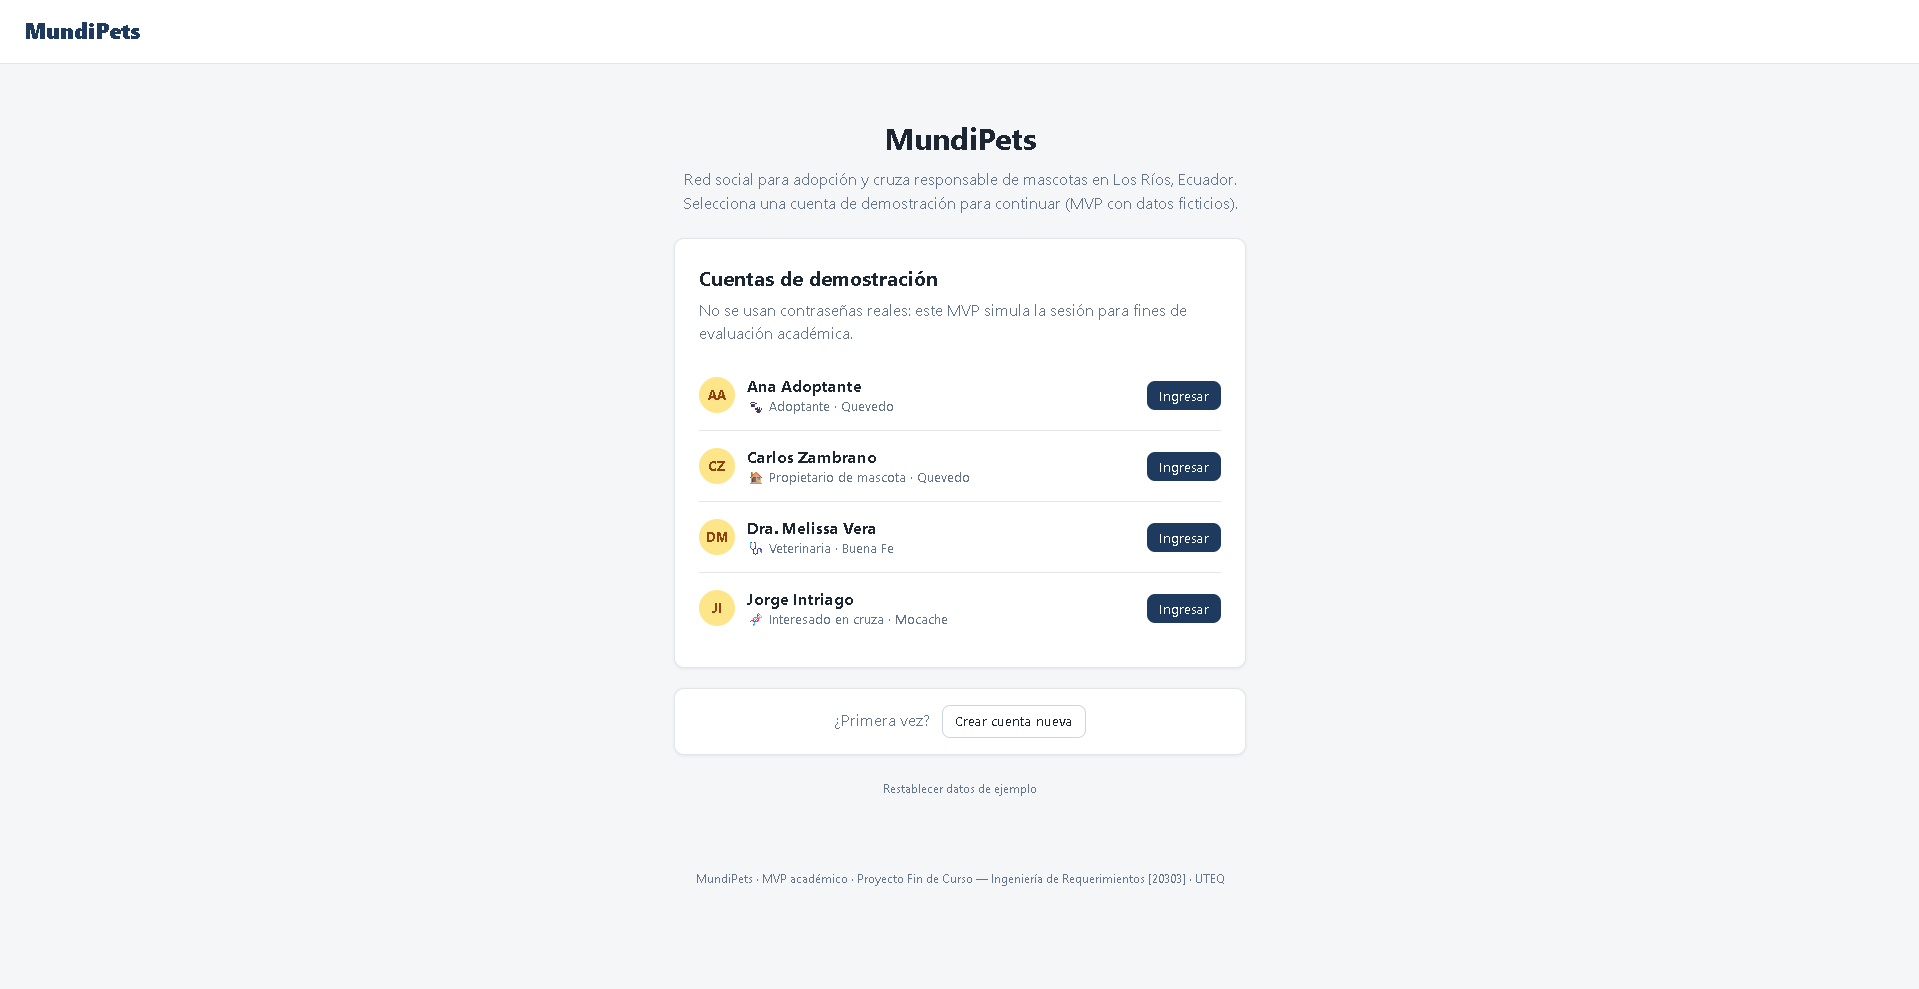
\includegraphics[width=0.92\textwidth]{figuras/MVP-01_InicioSesion_MundiPets.png}
		\caption{Pantalla de inicio de sesión del MVP (\texttt{index.html}). Se
			presentan las cuatro cuentas de demostración correspondientes a los roles
			del sistema --- Ana Adoptante, Carlos Zambrano (propietario), Dra. Melissa
			Vera (veterinaria) y Jorge Intriago (interesado en cruza) --- junto con la
			declaración explícita de que no se emplean contraseñas reales, que
			materializa la forma simulada de RF-12, y el enlace de restablecimiento
			de los datos de ejemplo.}
		\label{fig:mvp-login}
	\end{figure}
	
	\begin{figure}[H]
		\centering
		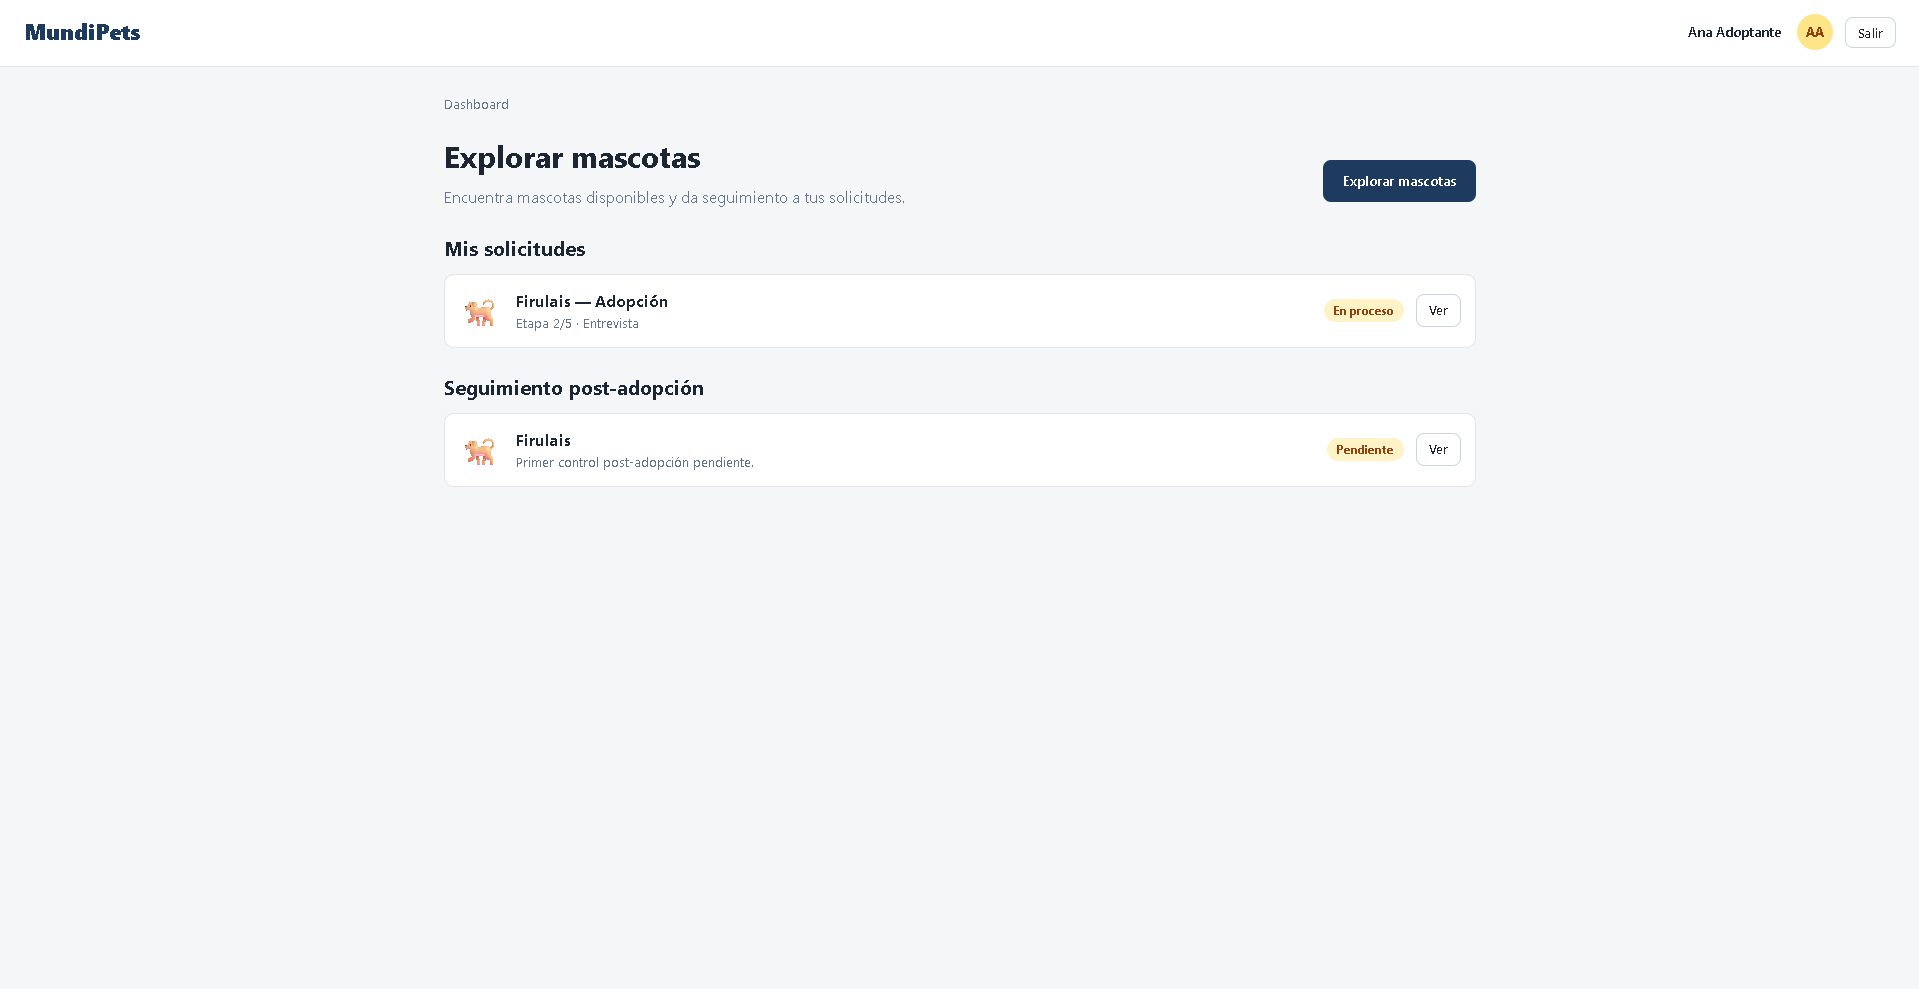
\includegraphics[width=0.92\textwidth]{figuras/MVP-02_PanelAdoptante_MundiPets.png}
		\caption{Panel de inicio diferenciado por rol (\texttt{dashboard.html}) para
			la cuenta de Ana Adoptante. La vista lista las solicitudes activas con su
			etapa vigente (\enquote{Etapa 2/5 --- Entrevista}) y los seguimientos
			post-adopción pendientes, evidenciando el acceso basado en roles de RD-02
			y los requisitos RF-18 y RF-22.}
		\label{fig:mvp-dashboard}
	\end{figure}
	
	\begin{figure}[H]
		\centering
		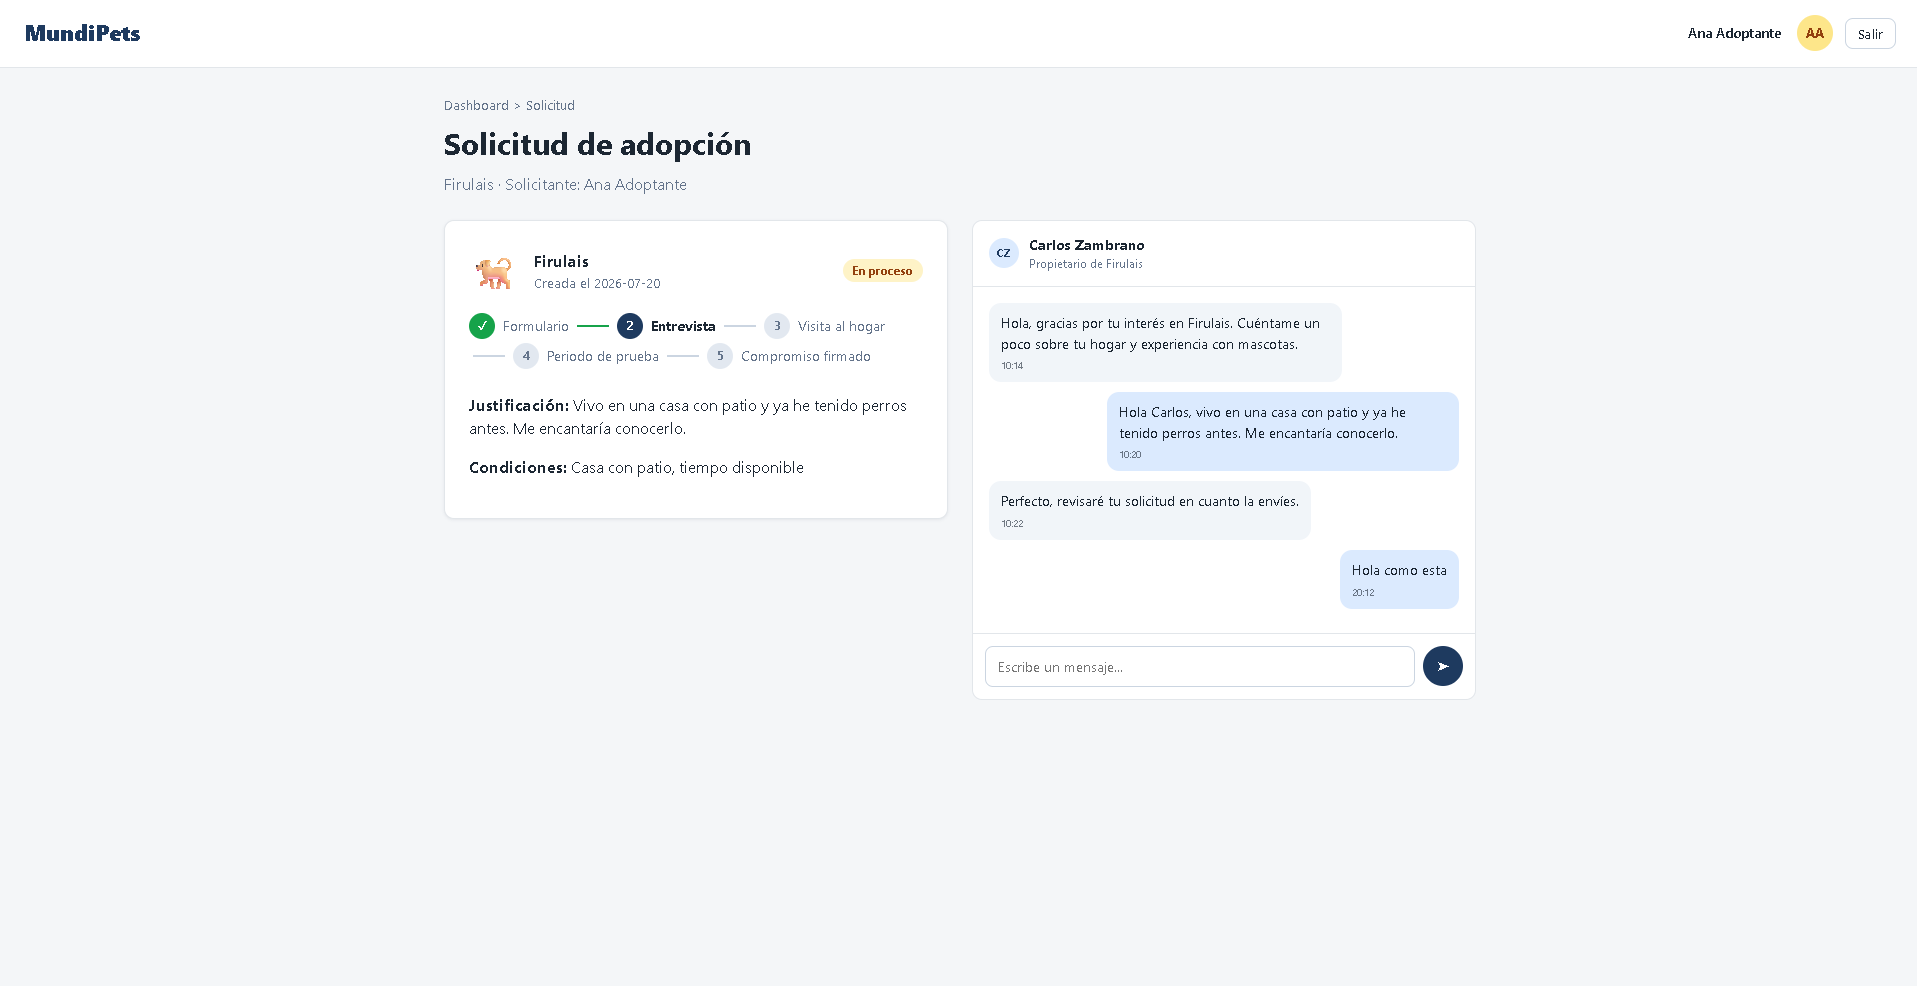
\includegraphics[width=0.92\textwidth]{figuras/MVP-03_SolicitudAdopcion_MundiPets.png}
		\caption{Detalle de una solicitud de adopción (\texttt{request.html}) con el
			indicador de las cinco etapas del proceso (formulario, entrevista, visita
			al hogar, periodo de prueba y compromiso firmado) y el panel de mensajería
			asociado a la solicitud, que implementan RF-05, RF-07 y RF-18.}
		\label{fig:mvp-solicitud}
	\end{figure}
	
	\begin{figure}[H]
		\centering
		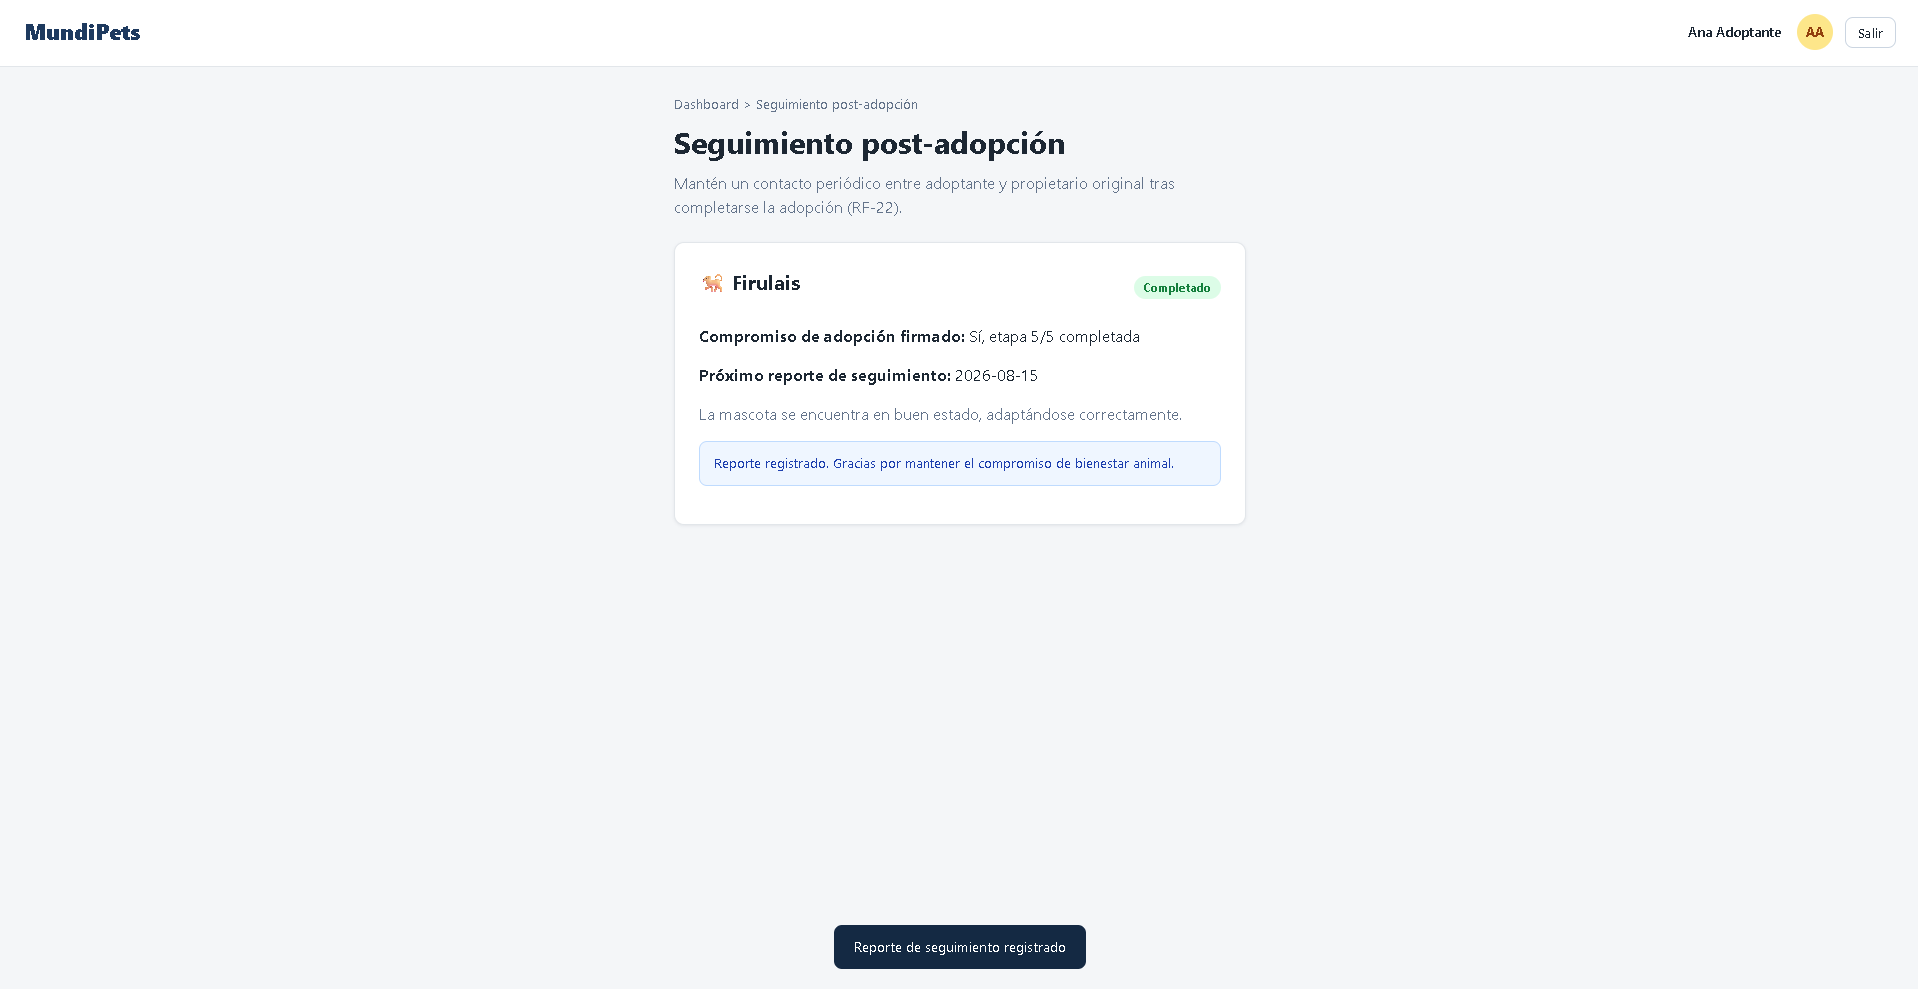
\includegraphics[width=0.92\textwidth]{figuras/MVP-04_SeguimientoPostAdopcion_MundiPets.png}
		\caption{Registro de seguimiento post-adopción (\texttt{post-adoption.html})
			generado automáticamente al completarse la quinta etapa de la solicitud.
			La vista muestra el compromiso firmado, la fecha del próximo reporte y el
			estado de la mascota adoptada, correspondientes a RF-22.}
		\label{fig:mvp-postadopcion}
	\end{figure}
	
	El video de recorrido funcional, de duración menor o igual a tres minutos,
	se encuentra en \texttt{05\_MVP/video\_demo.mp4}, y el enlace al repositorio
	público del MVP, junto con el commit exacto evaluado, se declara en
	\texttt{05\_MVP/README.md} y en el Apéndice~\ref{ap:repositorio}.
	
	% ############################################################
	%            SECCION 7 -- COMPONENTE EMPIRICO
	% ############################################################
	\section{Componente empírico del proyecto}
	\label{sec:empirico}
	
	\subsection{Enfoque seleccionado y justificación}
	\label{sec:enfoque}
	
	El equipo optó por el \textbf{Enfoque 2 --- Detectar automáticamente
		ambigüedad y malos olores en los requisitos}, descartando el Enfoque 1
	(comparación de la calidad de los RF frente a un LLM) y el Enfoque 3
	(validación de requisitos de explicabilidad del componente de IA).
	
	\textbf{Justificación en función del sistema.} MundiPets cuenta, desde la
	Entrega 2 (1B), con un corpus consolidado de especificación (17 RF, 8 RNF y
	5 restricciones de diseño), que constituye el insumo directo sobre el cual
	puede ejecutarse un detector de ambigüedad sin depender de instrumentos
	adicionales de recolección con usuarios externos al proyecto.
	
	\textbf{Justificación en función de los datos disponibles.} Como parte de la
	revisión y refinamiento del SRS parcial, el equipo ya efectuó un primer
	ejercicio de identificación manual de defectos de redacción sobre RF-01 a
	RF-17 y RNF-01 a RNF-08, detectando patrones de ambigüedad, terminología
	imprecisa y requisitos no verificables consistentes con los \emph{malos
		olores} descritos por Ferrari \emph{et al.} \cite{ferrari2016}. Este
	antecedente ofrece una base real sobre la cual diseñar y calibrar el
	detector automático, en lugar de partir desde cero.
	
	\textbf{Justificación en función del tiempo.} Independientemente del tiempo
	total disponible en el cronograma de la asignatura, el costo temporal de
	cada enfoque no depende solo de la duración del periodo, sino de la
	\emph{naturaleza de su ruta crítica}. Los Enfoques 1 y 3 dependen de
	reclutar y coordinar agendas con personas ajenas al equipo, lo cual introduce
	una latencia que no se reduce aunque se disponga de más semanas: el
	Enfoque 1 requiere entre tres y cinco personas evaluadoras externas
	dispuestas a calificar a ciegas dos conjuntos de al menos 50 RF cada uno, y
	el Enfoque 3 requiere doce participantes externos distribuidos en dos rondas
	de validación moderada, con la consiguiente necesidad de encontrar,
	convocar y agendar a cada uno. En ambos casos, el tiempo de ejecución queda
	sujeto a la disponibilidad de terceros, un factor fuera del control directo
	del equipo. El Enfoque 2, en cambio, mantiene su ruta crítica dentro del
	equipo: solo requiere tres personas expertas ya identificadas y la
	construcción de un detector automático (un script propio o una herramienta
	existente), ambas tareas ejecutables sin depender de la disponibilidad de
	terceros. Por esta razón, el Enfoque 2 ofrece el menor riesgo de cronograma
	de los tres, con independencia de cuántas semanas se le asignen.
	
	La decisión fue adoptada internamente por el equipo.
	
	\subsection{Preguntas de investigación en formato PICOC}
	\label{sec:rq}
	
	\begin{table}[H]
		\centering
		\caption{Preguntas de investigación estructuradas según el marco PICOC.}
		\label{tab:picoc}
		\small
		\begin{tabularx}{\textwidth}{@{}p{2.6cm} X@{}}
			\toprule
			\textbf{Elemento PICOC} & \textbf{Descripción} \\
			\midrule
			Población & Conjunto de requisitos funcionales (RF), no funcionales
			(RNF) y restricciones de diseño (RD) especificados para el sistema
			MundiPets, redactados según la plantilla de ocho atributos exigida
			por la asignatura y vigentes al momento de la ejecución del
			experimento. \\
			Intervención & Clasificación automática de cada requisito como
			\emph{ambiguo} o \emph{no ambiguo} mediante un detector basado en
			reglas, que identifica cuantificadores vagos, conjunciones
			múltiples que ocultan más de un requisito, voz pasiva y ausencia
			de criterio de verificación explícito. \\
			Comparación & Clasificación manual e independiente del mismo
			conjunto de requisitos, realizada por tres personas expertas en
			Ingeniería de Requisitos, sin conocimiento previo de la salida del
			detector (evaluación a ciegas). \\
			Resultado & Precisión, exhaustividad (\emph{recall}) y medida
			F1 del detector automático tomando como referencia el consenso
			experto; acuerdo inter-evaluador mediante $\kappa$ de Cohen entre
			pares de expertos y $\kappa$ de Fleiss para el conjunto de los
			tres. \\
			Contexto & Proyecto académico de la asignatura de Ingeniería de
			Requerimientos [20303] (UTEQ, 2026-2027 PPA), aplicado al sistema
			real MundiPets, con especificación redactada en español. \\
			\midrule
			RQ1 & ¿Con qué precisión, exhaustividad y medida F1 replica un
			detector automático basado en reglas el juicio consensuado de
			personas expertas al clasificar como ambiguos los requisitos
			especificados para MundiPets? \\
			RQ2 & ¿Qué patrones de desacuerdo predominan entre el detector
			automático y el juicio experto, y qué explican sobre las
			limitaciones de un enfoque basado en reglas frente al juicio
			humano en la identificación de ambigüedad? \\
			\bottomrule
		\end{tabularx}
	\end{table}
	
	\subsection{Hipótesis o proposiciones del estudio}
	\label{sec:hipotesis}
	
	Al tratarse del Enfoque 2, el diseño corresponde a un cuasi-experimento y
	requiere hipótesis nula y alternativa, no proposiciones de estudio de caso.
	
	\textbf{H\textsubscript{0} (hipótesis nula):} la clasificación producida
	por el detector automático de ambigüedad no guarda asociación con la
	clasificación de consenso de las personas expertas; el acuerdo observado
	entre ambas ($\kappa$ de Cohen) no es significativamente distinto del
	acuerdo esperado por azar ($\kappa = 0$).
	
	\textbf{H\textsubscript{1} (hipótesis alternativa):} la clasificación
	producida por el detector automático de ambigüedad guarda asociación
	significativa con la clasificación de consenso de las personas expertas;
	el acuerdo observado entre ambas es significativamente mayor que el
	esperado por azar ($\kappa > 0$).
	
	Esta hipótesis se contrasta mediante la prueba de significancia del
	$\kappa$ de Cohen descrita en la Sección \ref{sec:plan-analisis}. La
	pregunta RQ2, al ser de carácter exploratorio sobre los patrones de
	desacuerdo, no se somete a prueba de hipótesis: se responde mediante
	análisis cualitativo de los casos en los que el detector y el consenso
	experto difieren, siguiendo el sexto paso descrito para el Enfoque 2 en la
	guía de la asignatura.
	
	\subsection{Variables independientes, dependientes y de control}
	\label{sec:variables}
	
	\textbf{Variable independiente.} El método de clasificación aplicado a
	cada requisito, con dos niveles: (a) detector automático basado en reglas
	y (b) consenso de las tres personas expertas.
	
	\textbf{Variable dependiente.} La clasificación resultante de cada
	requisito como \emph{ambiguo} o \emph{no ambiguo} (variable categórica
	binaria), a partir de la cual se calculan las métricas de acuerdo
	declaradas en la Sección \ref{sec:plan-analisis} (precisión, exhaustividad,
	medida F1 y $\kappa$).
	
	\textbf{Variables de control.}
	\begin{itemize}[leftmargin=*]
		\item \textbf{Tipo de requisito} (RF, RNF o RD), para verificar que el
		desempeño del detector no varíe sistemáticamente según el tipo de
		artefacto evaluado.
		\item \textbf{Configuración fija del detector}: el conjunto de reglas
		(cuantificadores vagos, conjunciones múltiples, voz pasiva, ausencia de
		criterio de verificación) permanece invariable durante toda la
		ejecución del experimento; ninguna regla se ajusta después de observar
		resultados parciales.
		\item \textbf{Orden de presentación} de los requisitos a las personas
		expertas, aleatorizado de forma independiente para cada evaluador, con
		el fin de controlar efectos de fatiga o de orden.
		\item \textbf{Cegamiento del juicio experto}: ninguna persona
		evaluadora tiene acceso a la salida del detector ni a la clasificación
		de las demás personas evaluadoras antes de completar la propia.
	\end{itemize}
	
	\subsection{Participantes y reclutamiento}
	\label{sec:participantes}
	
	El estudio involucra dos grupos con roles distintos: las personas expertas
	que ejecutan la clasificación de referencia, y el equipo de MundiPets, que
	construye y aplica el detector automático sin participar en la
	clasificación experta, para preservar la independencia del juicio.
	
	\textbf{Personas expertas.} El panel está compuesto por tres Ingenieros de
	Software graduados de la Universidad Técnica Estatal de Quevedo (UTEQ) (dos
	mujeres y un hombre), ya contactados y confirmados para participar en el
	estudio.
	
	\textbf{Criterios de inclusión:} (a) título profesional de tercer nivel en
	Ingeniería de Software o carrera afín; (b) formación o experiencia
	demostrable en especificación y análisis de requisitos de software; (c)
	disponibilidad para completar la clasificación dentro del cronograma del
	estudio.
	
	\textbf{Criterios de exclusión:} (a) pertenecer al equipo de desarrollo de
	MundiPets; (b) haber participado en la redacción de los RF, RNF o RD que
	conforman la población del estudio (Sección \ref{sec:rq}).
	
	\textbf{Proceso de consentimiento informado.} Cada persona evaluadora firma
	un consentimiento informado específico para este rol, redactado en
	cumplimiento de la Ley Orgánica de Protección de Datos Personales del
	Ecuador \cite{lopdp2021}, que autoriza expresamente su participación como
	evaluadora experta y el uso de la clasificación producida --de forma
	anonimizada-- en publicaciones científicas revisadas por pares. La
	plantilla se detalla en la Sección \ref{sec:instrumentos}.
	
	\subsection{Instrumentos}
	\label{sec:instrumentos}
	
	Los instrumentos del Enfoque 2 son dos:
	
	\begin{enumerate}[leftmargin=*]
		\item \textbf{Rúbrica de clasificación experta}
		(\texttt{rubrica\_clasificacion\_experta.xlsx}): libro con hoja de
		instrucciones, hoja de criterios de referencia para identificar
		ambigüedad, y hoja de evaluación en la que cada persona evaluadora
		registra, para cada requisito, su identificador, el texto completo,
		la clasificación (\emph{ambiguo} / \emph{no ambiguo}), el tipo de
		mal olor detectado y una justificación breve. Los requisitos se
		presentan sin indicar su tipo (RF, RNF o RD) y en orden aleatorizado,
		para reducir sesgos de expectativa. Una hoja adicional, de uso
		exclusivo del equipo, conserva la clave que vincula cada identificador
		anónimo con el requisito real y la salida del detector.
		\item \textbf{Plantilla de consentimiento para evaluadores expertos}
		(\texttt{consentimiento\_evaluador\_experto.docx}): adapta el formato
		de consentimiento ya utilizado en la Entrega 1B para entrevistas,
		ajustado al rol de evaluador experto e incorporando la autorización
		explícita para el uso de datos anonimizados en publicaciones
		revisadas por pares, conforme a la LOPDP \cite{lopdp2021}.
	\end{enumerate}
	
	\subsection{Plan de análisis estadístico}
	\label{sec:plan-analisis}
	
	\textbf{Análisis principal (RQ1, H\textsubscript{0}/H\textsubscript{1}).}
	Se calculan precisión, exhaustividad y medida F1 del detector automático
	tomando como referencia el consenso experto (Sección \ref{sec:hipotesis}).
	La hipótesis se contrasta mediante una prueba de significancia del $\kappa$
	de Cohen (estadístico $z = \kappa / SE_{\kappa}$, contra la distribución
	normal estándar), mientras que la magnitud del acuerdo se interpreta como
	el tamaño del efecto, usando la escala de Landis y Koch: 0,00--0,20 leve;
	0,21--0,40 aceptable; 0,41--0,60 moderado; 0,61--0,80 sustancial;
	0,81--1,00 casi perfecto.
	
	\textbf{Acuerdo inter-evaluador.} $\kappa$ de Cohen \cite{cohen1960} para
	cada par de las tres personas expertas, y $\kappa$ de Fleiss
	\cite{fleiss1971} para el conjunto de las tres, interpretados con la misma
	escala de Landis y Koch. Un acuerdo experto bajo relativizaría cualquier
	conclusión sobre el desempeño del detector, ya que el propio consenso de
	referencia quedaría en duda.
	
	\textbf{Prueba de normalidad (Shapiro-Wilk).} Se aplica sobre la variable
	continua \emph{nivel de confianza} (escala 1--5) registrada en la rúbrica
	de evaluación (Sección \ref{sec:instrumentos}), como paso previo al
	análisis exploratorio secundario descrito a continuación.
	
	\textbf{Análisis secundario (RQ2, exploratorio).} Para caracterizar los
	casos de desacuerdo entre el detector y el consenso experto, se compara el
	nivel de confianza reportado por las personas expertas entre los
	requisitos donde el detector coincide con el consenso y aquellos donde
	difiere. Si Shapiro-Wilk no rechaza normalidad, se usa la prueba t de
	Student para muestras independientes y el tamaño del efecto se reporta
	como $d$ de Cohen; en caso contrario, se usa la prueba U de Mann-Whitney y
	el tamaño del efecto como $\delta$ de Cliff. Este análisis es exploratorio
	y se complementa con la nota cualitativa de desacuerdos exigida por el
	sexto paso del Enfoque 2 en la guía de la asignatura.
	
	\textbf{Corrección por comparaciones múltiples.} Si además se reportan
	métricas de acuerdo desagregadas por tipo de requisito (RF, RNF, RD) como
	análisis exploratorio adicional, los valores $p$ resultantes de esas tres
	comparaciones relacionadas se ajustan mediante el procedimiento de
	Benjamini-Hochberg (control de la tasa de falsos descubrimientos).
	
	\textbf{Cálculo de potencia estadística.} Conforme a Molléri \emph{et al.}
	\cite{molleri2020} y Wohlin \emph{et al.} \cite{wohlin2012}, se fija
	$\alpha = 0{,}05$ y $1 - \beta = 0{,}80$. Dado que el tamaño de la
	población está acotado por el corpus real de especificación disponible
	(Sección \ref{sec:enfoque}) y no por una meta de reclutamiento ampliable,
	el cálculo de potencia se reporta en sentido inverso: en lugar de fijar un
	$N$ objetivo, se determina la sensibilidad mínima (el valor mínimo de
	$\kappa$ detectable) que el diseño puede identificar con ese $\alpha$ y
	esa potencia, dado el $N$ realmente disponible al momento de la ejecución.
	Este cálculo se documentará con el valor real de $N$ y se versionará junto
	con el resto del análisis.
	
	\textbf{Reproducibilidad.} Todos los cálculos anteriores se ejecutan
	mediante scripts versionados en \texttt{06\_Experimento/scripts\_analisis/}
	(Python, con \texttt{SciPy}/\texttt{statsmodels} o R); ninguna cifra o
	tabla de esta sección se produce de forma manual, conforme a la regla de
	la guía de la asignatura.
	
	\subsection{Registro previo del protocolo en el OSF}
	\label{sec:osf}
	
	El protocolo del Enfoque 2 se registró en el Open Science Framework
	\cite{nosek2018}, mediante la plantilla \emph{OSF Preregistration}, el
	\textbf{27 de julio de 2026 a las 10:49:41 a.\,m.} (hora de Ecuador), antes
	de distribuir la rúbrica de clasificación al panel experto y antes de
	ejecutar el detector automático sobre el corpus de requisitos. El registro
	puede consultarse en:
	\url{https://osf.io/khyf2/overview}.
	El registro fue \textbf{aceptado} tras la moderación estándar de OSF
	posterior al envío. La marca de tiempo corresponde al momento del envío, en
	el que el contenido del registro queda congelado, con independencia de la
	fecha de aprobación.
	
	\subsection{Amenazas a la validez previstas}
	\label{sec:amenazas}
	
	\textbf{Validez interna.}
	\begin{itemize}[leftmargin=*]
		\item \emph{Sesgo de diseño del detector.} El equipo que construye el
		detector ya conoce, por la revisión manual previa realizada durante
		el refinamiento del SRS parcial (Sección \ref{sec:enfoque}), algunos
		de los defectos presentes en RF-01 a RF-17, lo que podría calibrar
		las reglas hacia esos casos conocidos e inflar artificialmente la
		precisión. \textbf{Mitigación:}
		las reglas del detector (Sección \ref{sec:enfoque}) se fijan y
		documentan antes de recibir la clasificación de los tres expertos
		sobre el conjunto completo, y se aplican sin modificación posterior
		(Sección \ref{sec:variables}). \textbf{Limitación reconocida:} el
		sesgo no se elimina por completo, porque el conocimiento previo del
		equipo sobre una parte del corpus es inevitable; se atenúa
		parcialmente al incluir en la población los RF-18 a RF-25, que no
		formaron parte de esa revisión previa.
		\item \emph{Efecto de orden o fatiga en la evaluación experta.}
		Evaluar un conjunto largo de requisitos de forma consecutiva puede
		degradar el juicio hacia el final del ejercicio. \textbf{Mitigación:}
		orden de presentación aleatorizado de forma independiente para cada
		evaluador (Sección \ref{sec:variables}). \textbf{Limitación
			reconocida:} la aleatorización distribuye el efecto pero no lo
		elimina; no se mide directamente si la fatiga afectó casos
		específicos.
	\end{itemize}
	
	\textbf{Validez externa.}
	\begin{itemize}[leftmargin=*]
		\item \emph{Corpus de un solo sistema y dominio.} Los requisitos
		provienen únicamente de MundiPets, redactados en español por un solo
		equipo estudiantil en el dominio veterinario/adopción de mascotas.
		\textbf{Mitigación:} el contexto queda documentado explícitamente en
		el marco PICOC (Sección \ref{sec:rq}) para que cualquier lector pueda
		evaluar la transferibilidad. \textbf{Limitación reconocida:} no puede
		afirmarse que el desempeño del detector generalice a otros dominios,
		idiomas o equipos con distinto nivel de experiencia; el estudio se
		declara como un caso único, no como una validación general del
		detector.
		\item \emph{Homogeneidad del panel experto.} Las tres personas
		evaluadoras son Ingenieras e Ingeniero de Software graduados de la
		misma universidad (UTEQ). \textbf{Mitigación:} el perfil exacto del
		panel se documenta en la Sección \ref{sec:participantes}.
		\textbf{Limitación reconocida:} no se garantiza representatividad de
		la diversidad de juicio experto que existiría con un panel de otras
		instituciones o con mayor trayectoria profesional.
	\end{itemize}
	
	\textbf{Validez de constructo.}
	\begin{itemize}[leftmargin=*]
		\item \emph{Binarización de un fenómeno gradual.} La ambigüedad
		rara vez es todo-o-nada; reducirla a \emph{ambiguo}/\emph{no ambiguo}
		simplifica un constructo más complejo. \textbf{Mitigación:} la
		rúbrica captura matices adicionales mediante el campo \emph{tipo de
			mal olor detectado} y el \emph{nivel de confianza} (Sección
		\ref{sec:instrumentos}). \textbf{Limitación reconocida:} la variable
		principal de análisis sigue siendo binaria; se acepta esta
		simplificación como necesaria para el análisis cuantitativo dentro
		del tiempo disponible.
		\item \emph{Alcance limitado de un detector basado en reglas.} El
		detector identifica ambigüedad léxica y sintáctica (cuantificadores
		vagos, voz pasiva, conjunciones múltiples), pero no ambigüedad
		semántica de dominio que solo una persona con conocimiento
		veterinario puede reconocer. \textbf{Mitigación:} el alcance de las
		reglas se documenta explícitamente y no se presenta el detector como
		un sustituto general del juicio experto. \textbf{Limitación
			reconocida:} la comparación mide específicamente cuánta ambigüedad
		\emph{detectable por reglas léxicas} coincide con el juicio experto
		global, no toda forma posible de ambigüedad.
	\end{itemize}
	
	\textbf{Validez de conclusión.}
	\begin{itemize}[leftmargin=*]
		\item \emph{Tamaño de muestra reducido.} La población disponible
		(Sección \ref{sec:enfoque}) es menor al mínimo de 50 requisitos
		sugerido por la guía de la asignatura para este enfoque, lo que
		reduce la potencia para detectar valores pequeños de $\kappa$ como
		significativamente distintos de cero. \textbf{Mitigación:} el plan
		de análisis (Sección \ref{sec:plan-analisis}) reporta explícitamente
		la sensibilidad mínima detectable dado el $N$ real, en vez de ocultar
		la limitación. \textbf{Limitación reconocida:} con un $N$ reducido,
		el estudio puede no tener potencia suficiente para detectar niveles
		de acuerdo moderados-bajos como estadísticamente significativos; los
		resultados de la Entrega 4 deberán interpretarse con este límite en
		mente.
		\item \emph{Panel experto mínimo.} Solo tres personas conforman el
		consenso de referencia, el mínimo aceptado por la guía; con un panel
		tan pequeño, la opinión de una sola persona pesa proporcionalmente
		más sobre el consenso. \textbf{Mitigación:} se calcula
		explícitamente el acuerdo inter-evaluador mediante $\kappa$ de Fleiss
		antes de aceptar el consenso como válido. \textbf{Limitación
			reconocida:} un panel de tres es más vulnerable a la idiosincrasia
		individual que el panel de cinco recomendado por la guía, al que no
		se llega por restricciones de tiempo.
	\end{itemize}
	
	% ############################################################
	%                    SECCION 8 -- CONCLUSIONES
	% ############################################################
	
	% ############################################################
	%                    SECCION 8 -- CONCLUSIONES
	% ############################################################
	\section{Conclusiones}
	\label{sec:conclusiones}
	
	Esta entrega consolida la Especificación de Requisitos de Software de
	MundiPets como un documento completo, verificable y sustentado en evidencia
	de campo. El resultado principal es que la totalidad de los requisitos
	especificados --- 25 requisitos funcionales, 16 no funcionales y 9
	restricciones de diseño --- queda trazada hasta al menos una evidencia
	primaria del catálogo del Apéndice~B.1, y ninguna afirmación sustantiva del
	documento se apoya únicamente en la deliberación interna del equipo.
	
	\paragraph{Sobre la completitud de la especificación.}
	La segunda ronda de campo amplió el corpus de evidencias de 8 a 22 unidades,
	incorporando entrevistas adicionales, un cuestionario con 38 respuestas
	válidas y cuatro sesiones de validación \emph{walkthrough} con usuarios
	técnicos y no técnicos. La curva de saturación temática
	(Sección~\ref{sec:codificacion}) alcanza cero códigos nuevos en la evidencia
	EV-17, lo que indica que el corpus de elicitación llegó al punto de
	saturación antes de cerrar la ronda. Los ocho requisitos incorporados en esta
	entrega (RF-18 a RF-25) no surgieron de una revisión de escritorio sino de
	necesidades expresadas por participantes concretos, lo que explica que la
	especificación crezca sin que la saturación se vea contradicha: las
	entrevistas finales aportaron matices sobre categorías ya identificadas más
	que categorías nuevas.
	
	\paragraph{Sobre el marco legal y la explicabilidad.}
	El mapeo de la Ley Orgánica de Protección de Datos Personales del Ecuador
	\cite{lopdp2021} contra los requisitos (Sección~\ref{sec:legales}) mostró que
	el marco legal no es un anexo del diseño sino una fuente de requisitos por
	derecho propio: el Art.~20, sobre decisiones automatizadas, es la base
	directa de los tres requisitos de explicabilidad (RNF-13, RNF-14 y RNF-15),
	que de otro modo se habrían tratado como una preocupación de usabilidad. La
	decisión de tratar la explicabilidad como requisito no funcional medible,
	siguiendo a Chazette y Schneider \cite{chazette2020}, obligó a definir
	métricas concretas --- extensión máxima de la explicación, tiempo de
	generación y comprensión reportada --- en lugar de enunciados genéricos sobre
	transparencia.
	
	\paragraph{Sobre las limitaciones reconocidas.}
	El documento declara de forma expresa aquello que no pudo establecerse con
	los datos disponibles. La clasificación según el modelo de Kano no se derivó
	porque el cuestionario v2.0 midió importancia declarada pero no incluyó el
	par de preguntas funcional y disfuncional que el modelo exige
	(Sección~\ref{sec:kano}); en su lugar se reporta una aproximación rotulada
	como tal. Del mismo modo, tres requisitos funcionales de prioridad
	\emph{Must} (RF-18, RF-22 y RF-23) aún no cuentan con prototipo de interfaz
	asociado. Reconocer estos límites es preferible a presentarlos como
	resueltos, y ambos quedan como trabajo inmediato.
	
	\paragraph{Sobre el componente empírico.}
	El protocolo del estudio de detección automática de ambigüedad quedó
	registrado en el Open Science Framework antes de iniciar la recolección de
	datos, lo que fija la marca temporal del diseño con independencia de los
	resultados obtenidos. Esta decisión metodológica es la que permitirá, en la
	Entrega 4, reportar los hallazgos sin sospecha de ajuste posterior de las
	hipótesis.
	
	\paragraph{Trabajo inmediato.}
	Las prioridades para el cierre del semestre son cuatro: completar los tres
	prototipos de interfaz pendientes; ampliar el instrumento a una versión v3.0
	que habilite la clasificación Kano; ejecutar el plan de análisis estadístico
	completo sobre los datos ya recolectados; y consolidar el paquete de datos
	anonimizado para su depósito con identificador persistente, siguiendo los
	principios FAIR \cite{wilkinson2016} y las prácticas de citación de software
	\cite{smith2016}.
	
	% ############################################################
	%                        REFERENCIAS
	% ############################################################
	\newpage
	\printbibliography[title={Referencias}]
	\addcontentsline{toc}{section}{Referencias}
	
	% ############################################################
	%                        APENDICES
	% ############################################################
	\newpage
	\appendix
	
	% --------------------------------------------------------
	\section*{Apéndice A --- Plan del proyecto de IR}
	\addcontentsline{toc}{section}{Apéndice A --- Plan del proyecto de IR}
	\label{ap:plan}
	
	\textbf{Roles del equipo (vigentes para la Entrega 3, 2A):}
	
	\begin{table}[H]
		\caption{Roles asignados al equipo del proyecto MundiPets.}
		\centering
		\begin{tabularx}{\linewidth}{|X|X|}
			\hline
			\textbf{Integrante} & \textbf{Rol} \\
			\hline
			Fuertes Arraes Edson Daniel & Analista líder -- coordina el equipo, valida con el cliente, redacta los requisitos funcionales e historias de usuario, gestiona el repositorio. \\
			\hline
			Gutiérrez Ortega Génesis Adriana & Verificador -- controla la calidad de los requisitos no funcionales, la explicabilidad, el marco legal y las evidencias de campo. \\
			\hline
			Mendoza Párraga Andy Johel & Modelador -- construye los ocho diagramas UML exigidos y los mockups de alta fidelidad. \\
			\hline
			Morales Sánchez Gary Alejandro & Documentador -- estructura el ERS/SRS según IEEE 29148, contexto, modelado organizacional y trazabilidad. \\
			\hline
			Nieves Sánchez Jimmy Samuel & Verificador -- responsable del componente empírico, el MVP y el paquete de publicación. \\
			\hline
		\end{tabularx}
	\end{table}
	
	\textbf{Cronograma del proyecto (actualizado a la Entrega 3, 2A):}
	
	\begin{table}[H]
		\caption{Cronograma de la Ingeniería de Requisitos -- MundiPets (Semestre 2026-2027 PPA).}
		\centering
		
		\begin{tabularx}{\linewidth}{|C{2.5cm}|X|C{2.8cm}|}
			\hline
			\textbf{Semana / Fecha} & \textbf{Actividad} & \textbf{Estado} \\
			\hline
			Semanas 1--3 (04--24 may.) & Selección del sistema real (MundiPets), planificación de la Ingeniería de Requisitos y definición de roles del equipo. & Completado \\
			\hline
			\textbf{Semana 4 (25--31 may.)} & \textbf{Primer avance:} Planificación + Elicitación inicial (Entrega 1A). Ejecución de entrevistas estructuradas a stakeholders (17--29 may.). & Completado \\
			\hline
			Semanas 5--8 (01--28 jun.) & Consolidación de requisitos crudos, análisis y clasificación (RF/RNF/restricciones), modelado UML inicial (casos de uso y clases conceptual). & Completado \\
			\hline
			\textbf{Semana 9 (29 jun.--05 jul.)} & \textbf{Segundo avance:} ERS/SRS parcial -- requisitos formalizados (plantilla de 8 atributos), RNF cuantificados, modelado UML e interfaces, priorización MoSCoW y trazabilidad parcial (Entrega 2/1B). & Completado \\
			\hline
			Semanas 10--11 (06--19 jul.) & Segunda ronda de elicitación: entrevistas y sesiones de walkthrough adicionales, ampliación del cuestionario (v2.0) para cubrir Kano, codificación temática de las transcripciones y curva de saturación. & Completado \\
			\hline
			Semana 12 (20--26 jul.) & Redacción de los RF-18 a RF-25 y RNF-09 a RNF-15 a partir de la codificación temática, mapeo legal LOPDP, construcción del diagrama de Razón Estratégica (SR) y refinamiento del diagrama de clases. & Completado \\
			\hline
			\textbf{Semana 13 (27 jul.--02 ago.)} & \textbf{Tercer avance:} ERS Completo con Validación y Trazabilidad -- documento de especificación de requisitos completo, validado y con trazabilidad total evidencia--requisito--caso de uso, priorización Kano/WSJF, MVP y protocolo del componente empírico registrado en el OSF. & Completado \\
			\hline
			Semanas 14--16 (03--23 ago.) & Ejecución del componente empírico, desarrollo del MVP, revisión integral del documento y ajustes finales según observaciones del docente. & Planificado \\
			\hline
			\textbf{Semana 17 (24--30 ago.)} & \textbf{Cuarto avance:} Proyecto Integrador Final -- entrega y sustentación del documento ERS/SRS completo del Proyecto Fin de Curso. & Planificado \\
			\hline
		\end{tabularx}
	\end{table}
	
	\textbf{Técnicas de elicitación seleccionadas:}
	
	Para esta entrega se mantiene la entrevista estructurada como técnica
	principal, complementada con sesiones de \emph{walkthrough} para la
	validación de los requisitos ya especificados. La segunda ronda de campo
	amplía el cuestionario aplicado en la 1B (versión 2.0) con las preguntas
	funcional y disfuncional del modelo de Kano para cada funcionalidad candidata,
	de modo que la priorización Kano de la Sección~\ref{sec:kano} quede
	respaldada por datos reales y no por criterio de escritorio. Esta técnica se
	complementa con la codificación temática de las transcripciones
	(Apéndice~B.8), que es el insumo directo para derivar los ocho requisitos
	funcionales nuevos (RF-18 a RF-25) exigidos por esta entrega.
	
	% --------------------------------------------------------
	\section*{Apéndice B --- Trabajo de campo y evidencias}
	\addcontentsline{toc}{section}{Apéndice B --- Trabajo de campo y evidencias}
	\label{ap:evidencias}
	
	\subsection*{B.1 Registro y catálogo de evidencias}
	
	La Tabla~\ref{tab:catalogo-evidencias} consolida las veintidós evidencias de campo
	recogidas por el equipo, indicando el tipo de instrumento aplicado, el participante
	o fuente, los requisitos derivados de cada una y si se cuenta con el consentimiento
	informado firmado correspondiente (Apéndice~B.6).
	
	\textbf{Codificación de participantes.} En cumplimiento de la restricción
	RD-09 y de la Ley Orgánica de Protección de Datos Personales del Ecuador
	\cite{lopdp2021}, ninguna persona participante se identifica por su nombre
	en este documento ni en los artefactos públicos del repositorio. Se emplean
	códigos de participante con el prefijo \texttt{PROP-XX} para propietarios de
	mascota, \texttt{VET-XX} para profesionales veterinarios y \texttt{OBS-XX}
	para establecimientos observados. La tabla de correspondencia entre código y
	persona real no se publica: permanece en la zona restringida
	(\texttt{02\_Evidencias/00\_Restringido/}) bajo custodia del equipo y del
	docente responsable. Una misma persona puede estar asociada a más de una
	evidencia; por ejemplo, quien participó en una entrevista y posteriormente
	en una sesión de validación conserva el mismo código.
	
	{\small
		\begin{longtable}{@{}>{\raggedright\arraybackslash}p{1.2cm} >{\raggedright\arraybackslash}p{3.1cm} >{\raggedright\arraybackslash}p{3.1cm} >{\raggedright\arraybackslash}p{6.0cm} >{\raggedright\arraybackslash}p{1.4cm}@{}}
			\caption{Registro y catálogo de evidencias del trabajo de campo.}
			\label{tab:catalogo-evidencias}\\
			\toprule
			\textbf{ID-EV} & \textbf{Tipo de evidencia} & \textbf{Fuente / participante} & \textbf{Requisitos derivados} & \textbf{Consent.} \\
			\midrule
			\endfirsthead
			\multicolumn{5}{@{}l}{\small\itshape (continuación)}\\
			\toprule
			\textbf{ID-EV} & \textbf{Tipo de evidencia} & \textbf{Fuente / participante} & \textbf{Requisitos derivados} & \textbf{Consent.} \\
			\midrule
			\endhead
			\bottomrule
			\endlastfoot
			EV-01 & Entrevista grabada, audio, video y consentimiento & PROP-01 (propietario de mascota) & RF-01, RF-03, RF-05, RF-07, RF-08, RF-12, RF-13 & Sí \\
			\addlinespace
			EV-02 & Entrevista grabada, audio, video y consentimiento & PROP-02 (propietaria de mascota) & RF-01, RF-02, RF-03, RF-05, RF-07, RF-08, RF-10, RF-11, RF-13, RF-14, RF-15 & Sí \\
			\addlinespace
			EV-03 & Entrevista grabada, audio, video y consentimiento & VET-01 (médica veterinaria) & RF-01, RF-02, RF-05, RF-06, RF-08, RF-09, RF-12, RF-14, RF-16, RF-17, RNF-01, RNF-05, RNF-06, RNF-07, RD-03, RD-04 & Sí \\
			\addlinespace
			EV-04 & Entrevista grabada, audio, video y consentimiento & VET-02 (veterinario) & RF-02, RF-03, RF-06, RF-10, RF-13, RF-15, RNF-06, RNF-08, RD-03 & Sí \\
			\addlinespace
			EV-05 & Entrevista grabada, audio, video y consentimiento & VET-03 (médico veterinario) & RF-01, RF-02, RF-03, RF-05, RF-06, RF-08, RF-09, RF-11, RF-13, RF-14, RF-16, RF-17, RNF-01, RNF-05, RD-03, RD-04 & Sí \\
			\addlinespace
			EV-06 & Entrevista grabada, audio, video y consentimiento & PROP-03 (propietaria de mascota) & RF-01, RF-02, RF-03, RF-05, RF-08, RF-10, RF-11, RF-13, RF-14, RF-15 & Sí \\
			\addlinespace
			EV-07 & Cuestionario digital, formularios y resultados exportados & Usuarios potenciales encuestados & RF-01, RF-03, RF-04, RF-06, RF-07, RF-08, RF-11, RF-12, RF-13, RF-17, RNF-03, RNF-04, RNF-07 & No \\
			\addlinespace
			EV-08 & Observación presencial del proceso actual en una clínica veterinaria, con fotografías fechadas del entorno y consentimiento informado firmado por la veterinaria observada & OBS-01 (establecimiento veterinario) & RF-01, RF-03, RF-04, RF-05, RF-06, RF-07, RF-11, RF-12, RF-13, RF-17, RNF-01, RNF-04 & Si \\
			\addlinespace
			EV-09 & Entrevista grabada, audio, video y consentimiento & PROP-04 (propietario de mascota) & RF-11, RF-12, RF-23, RNF-09 & Si \\
			\addlinespace
			EV-10 & Entrevista grabada, audio, video y consentimiento & PROP-05 (propietario de mascota) & RF-11, RF-14, RF-22 & Si \\
			\addlinespace
			EV-11 & Entrevista grabada, audio, video y consentimiento & PROP-06 (propietaria de mascota) & RF-06, RF-10, RF-18, RF-19, RNF-13 & Sí \\
			\addlinespace
			EV-12 & Entrevista grabada, audio, video y consentimiento & PROP-07 (propietaria de mascota) & RF-23, RF-25 & Sí \\
			\addlinespace
			EV-13 & Entrevista grabada, audio, video y consentimiento & PROP-08 (propietario de mascota) & RF-06, RF-20, RNF-13 & Sí \\
			\addlinespace
			EV-14 & Entrevista grabada, audio, video y consentimiento & PROP-09 (propietario de mascota) & RF-03, RF-06, RF-11, RF-16 & Sí \\
			\addlinespace
			EV-15 & Entrevista grabada, audio, video y consentimiento & VET-04 (veterinaria) & RF-02, RF-09, RF-16, RF-23, RF-24, RNF-13 & Sí \\
			\addlinespace
			EV-16 & Entrevista grabada, audio, video y consentimiento & VET-05 (veterinario) & RF-02, RF-09, RF-14, RF-18, RF-21, RF-22, RF-24, RNF-13 & Sí \\
			\addlinespace
			EV-17 & Entrevista grabada, audio, video y consentimiento & PROP-10 (propietaria de mascota) & Refuerza RNF-13 & Sí \\
			\addlinespace
			EV-18 & Entrevista grabada, audio, video y consentimiento & PROP-11 (propietaria de mascota) & RF-11, RF-23, RNF-09, RD-04 & Sí \\
			\addlinespace
			EV-19 & Sesión de validación (\emph{walkthrough}) grabada en video & PROP-08 (propietario de mascota, usuario no técnico) & Validación de RF-01 a RF-17 & Sí \\
			\addlinespace
			EV-20 & Sesión de validación (\emph{walkthrough}) grabada en video & PROP-02 (propietaria de mascota, usuaria no técnica) & Validación de RF-01 a RF-08, RF-11 a RF-17 & Sí \\
			\addlinespace
			EV-21 & Sesión de validación (\emph{walkthrough}) grabada en video, con consentimiento & VET-04 (veterinaria, usuaria técnica) & Validación de RF-01 a RF-08, RF-11 a RF-17 & Sí \\
			\addlinespace
			EV-22 & Sesión de validación (\emph{walkthrough}) grabada en video, con consentimiento & VET-06 (veterinario, usuario técnico) & Validación de RF-01 a RF-17 & Sí \\
			\addlinespace
		\end{longtable}
	}
	
	\subsection*{B.2 Guion y guía de entrevista v2.0}
	
	Se emplearon dos guiones diferenciados según el perfil del participante. La
	Guía~A se aplicó a dueños de mascota y usuarios potenciales; la Guía~B, a
	profesionales veterinarios.
	
	\subsubsection*{Guía A --- Dueños de mascota y usuarios potenciales}
	
	\textbf{Objetivo:} conocer los riesgos, la información relevante y las
	consideraciones éticas para el desarrollo de una solución a la problemática.\\
	\textbf{Duración estimada:} 15--20 minutos.\\
	\textbf{Modalidad:} videollamada, con grabación de audio y video previo
	consentimiento informado (Apéndice~B.6).\\
	\textbf{Instrucciones para el entrevistador:} leer y hacer firmar el
	consentimiento informado antes de iniciar la grabación; formular las preguntas en
	el orden dado, permitiendo respuestas abiertas.
	
	\begin{enumerate}[leftmargin=*, itemsep=1pt]
		\item ¿Cómo suele conocer el estado de salud de su mascota?
		\item ¿Qué información considera necesaria antes de dejar a su mascota interactuar con otras mascotas?
		\item ¿Cómo suele realizar el seguimiento de vacunas o controles veterinarios?
		\item ¿Qué información considera privada o sensible sobre su mascota?
		\item ¿Qué información considera necesaria sobre el historial médico de una mascota?
		\item ¿Qué información considera más importante conocer sobre una mascota antes de adoptarla?
		\item ¿Qué problemas considera más comunes en procesos de adopción?
		\item ¿Qué factores influyen en su decisión al momento de elegir una mascota?
		\item ¿Cómo decide si una mascota es compatible con otra?
		\item ¿Qué aspectos considera importantes antes de permitir el cruce entre mascotas?
	\end{enumerate}
	
	\subsubsection*{Guía B --- Veterinarios y veterinarias}
	
	\textbf{Objetivo:} conocer los riesgos, la información relevante y las
	consideraciones éticas desde el criterio clínico-profesional.\\
	\textbf{Duración estimada:} 15--25 minutos.\\
	\textbf{Modalidad:} videollamada, con grabación de audio y video previo
	consentimiento informado (Apéndice~B.6).\\
	\textbf{Instrucciones para el entrevistador:} las mismas que en la Guía~A. Esta
	guía profundiza en el criterio clínico-profesional que complementa la perspectiva
	de los propietarios recogida en la Guía~A.
	
	\begin{enumerate}[leftmargin=*, itemsep=1pt]
		\item ¿Qué información considera más importante conocer sobre una mascota?
		\item ¿Qué datos ayudan a entender mejor el estado general de una mascota?
		\item ¿Qué antecedentes considera importantes conocer sobre una mascota?
		\item ¿Qué riesgos existen cuando no se conoce suficiente información sobre una mascota?
		\item ¿Cómo influye la edad de una mascota en su cuidado y comportamiento?
		\item ¿Cómo influye la raza en las necesidades de una mascota?
		\item ¿Qué datos de la mascota considera sensibles?
		\item ¿Qué enfermedades o condiciones considera importante registrar en una mascota?
		\item ¿Qué información involucra el perfil médico de una mascota?
		\item ¿Cómo puede verificarse si una mascota cuenta con controles médicos adecuados?
		\item ¿Cómo evalúa si una adopción puede considerarse responsable?
		\item ¿Qué información considera importante antes de entregar una mascota en adopción?
		\item ¿Cómo afectan las adopciones informales al bienestar animal?
		\item ¿Qué información considera esencial antes de recomendar un cruce entre mascotas?
		\item ¿Cómo puede identificarse si dos mascotas son compatibles entre sí?
		\item ¿Cómo identifica posibles riesgos en procesos de reproducción entre mascotas?
		\item ¿Cómo afectan los cruces irresponsables a las mascotas?
	\end{enumerate}
	
	
	\subsection*{B.3 Actas de entrevista firmadas}
	
	Se levantó un acta por cada entrevista de la segunda ronda de campo. Cada
	acta registra la fecha, el código de participante, el rol, la persona
	entrevistadora y la técnica aplicada, seguidos del resumen de preguntas y
	respuestas. Los originales firmados residen en la zona restringida del
	repositorio y las copias enmascaradas en
	\texttt{02\_Evidencias/Validacion\_Walkthrough/} y
	\texttt{02\_Evidencias/Documentos\_Organizacion/}. En cumplimiento de la
	RD-09, las personas entrevistadas se identifican únicamente por su código.
	
	
	\subsubsection*{Acta de entrevista 9 --- PROP-04}
	
	\begin{table}[H]
		\centering\small
		\begin{tabularx}{\textwidth}{@{}l X@{}}
			\toprule
			\textbf{Campo} & \textbf{Información} \\
			\midrule
			
			Fecha & 26/07/2026 \\
			
			Entrevistado & PROP-04 \\
			
			Cargo/Rol & Dueño de mascota \\
			
			Entrevistador & Fuertes Arraes Edson Fuertes \\
			
			Técnica & Entrevista semiestructurada \\
			
			\bottomrule
		\end{tabularx}
	\end{table}
	
	{\small
		\begin{longtable}{@{}p{5.6cm} p{9.4cm}@{}}
			\toprule
			\textbf{Pregunta} & \textbf{Respuesta resumida} \\
			\midrule
			\endfirsthead
			\multicolumn{2}{@{}l}{\small\itshape (continuación del acta 9)}\\
			\toprule
			\textbf{Pregunta} & \textbf{Respuesta resumida} \\
			\midrule
			\endhead
			\bottomrule
			\endlastfoot
			
			¿Cómo suele conocer el estado de salud de su mascota? & Identifica el estado de salud por cambios en la conducta habitual: sus mascotas se muestran distantes y decaídas cuando enferman. Interpreta las señales de forma individual (quietud en la hembra, normalmente activa; no acudir al llamado en el macho, de temperamento calmado) y considera que la prevención debe anteceder a la enfermedad. \\ \addlinespace
			
			¿Qué información considera necesaria antes de dejar a su mascota interactuar con otras mascotas? & Que el otro animal no sea agresivo ni tenga una diferencia de tamaño considerable (riesgo de peleas y lesiones), y que no presente signos evidentes de enfermedades contagiosas como moquillo o sarna. \\ \addlinespace
			
			¿Cómo suele realizar el seguimiento de vacunas o controles veterinarios? & Realiza chequeos preventivos cada seis a ocho meses, mantiene el esquema de vacunación de cachorro y esterilizó a la hembra. Trata de inmediato afecciones menores (pulgas, garrapatas). Señala el tiempo como su mayor dificultad y, en segundo lugar, el costo económico en casos graves. \\ \addlinespace
			
			¿Qué información considera privada o sensible sobre su mascota? & La existencia de enfermedades transmisibles (moquillo, sarna), por el estigma social que generan; su divulgación entre vecinos ha derivado históricamente en casos de animales envenenados, por lo que prefiere gestionar de inmediato la atención profesional. \\ \addlinespace
			
			¿Qué información considera necesaria sobre el historial médico de una mascota? & El registro de alergias, dato vital porque condiciona la elección del medicamento; también el historial de vacunas y desparasitaciones, enfermedades congénitas y enfermedades contagiosas. \\ \addlinespace
			
			¿Qué información considera más importante conocer sobre una mascota antes de adoptarla? & La condición de salud, el estado de vacunación, el peso y la edad. Prefiere animales jóvenes o recién nacidos por la facilidad de vínculo y se declara indiferente respecto de la raza. \\ \addlinespace
			
			¿Qué problemas considera más comunes en procesos de adopción? & La falta de transparencia de algunos albergues sobre edad, vacunación o desparasitación (por saturación y falta de financiamiento fijo); casos de mascotas que superan el tamaño anunciado; y estafas en adopciones en línea con cobros sucesivos por envío e implementos. \\ \addlinespace
			
			¿Qué factores influyen en su decisión al momento de elegir una mascota? & El estado de vacunación, la existencia de enfermedades de nacimiento y la edad del animal. No considera la raza un criterio determinante y prefiere ejemplares jóvenes. \\ \addlinespace
			
			¿Cómo decide si una mascota es compatible con otra? & Atribuye la compatibilidad a la crianza recibida: el maltrato genera agresividad, mientras que la alimentación, el afecto y el espacio para liberar estrés generan sociabilidad. Verifica mediante un encuentro supervisado, observando el lenguaje corporal (olfateo y juego). \\ \addlinespace
			
			¿Qué aspectos considera importantes antes de permitir el cruce entre mascotas? & Conocer previamente al dueño del otro ejemplar, su residencia y las condiciones de la vivienda; revisar el historial de vacunas y médico completo descartando enfermedades contagiosas; rechaza cruces entre tamaños dispares y condena la explotación reproductiva con fines comerciales. \\ \addlinespace
			
		\end{longtable}
	}
	
	
	\subsubsection*{Acta de entrevista 10 --- PROP-05}
	
	\begin{table}[H]
		\centering\small
		\begin{tabularx}{\textwidth}{@{}l X@{}}
			\toprule
			\textbf{Campo} & \textbf{Información} \\
			\midrule
			
			Fecha & 26/07/2026 \\
			
			Entrevistado & PROP-05 \\
			
			Cargo/Rol & Dueño de mascota \\
			
			Entrevistador & Fuertes Arraes Edson Fuertes \\
			
			Técnica & Entrevista semiestructurada \\
			
			\bottomrule
		\end{tabularx}
	\end{table}
	
	{\small
		\begin{longtable}{@{}p{5.6cm} p{9.4cm}@{}}
			\toprule
			\textbf{Pregunta} & \textbf{Respuesta resumida} \\
			\midrule
			\endfirsthead
			\multicolumn{2}{@{}l}{\small\itshape (continuación del acta 10)}\\
			\toprule
			\textbf{Pregunta} & \textbf{Respuesta resumida} \\
			\midrule
			\endhead
			\bottomrule
			\endlastfoot
			
			¿Cómo suele conocer el estado de salud de su mascota? & Tras años de convivencia, reconoce el estado de salud por el ánimo y los hábitos cotidianos (menor apetito, menor actividad, desinterés por el juego). Observa de medio día a un día para descartar un malestar momentáneo antes de acudir al veterinario. \\ \addlinespace
			
			¿Qué información considera necesaria antes de dejar a su mascota interactuar con otras mascotas? & Tener certeza de que el otro animal no padezca enfermedades de contacto directo (sarna, pulgas) y evitar animales de conducta agresiva. \\ \addlinespace
			
			¿Cómo suele realizar el seguimiento de vacunas o controles veterinarios? & Lleva un registro manual en una libreta con las vacunas y la fecha de esterilización, con controles cada seis meses. El método es frágil (ha extraviado la libreta varias veces); enfrenta dificultades de tiempo y costo (esperas de 3-4 horas, gastos superiores a \$50) y no cuenta con una veterinaria fija, lo que fragmenta el historial de su mascota. \\ \addlinespace
			
			¿Qué información considera privada o sensible sobre su mascota? & Postura mayoritariamente abierta, pues considera que la información de salud puede beneficiar al animal ante un problema médico. Delimita como sensibles el tipo de sangre y las enfermedades que podrían afectarlo, a compartir solo con el veterinario. \\ \addlinespace
			
			¿Qué información considera necesaria sobre el historial médico de una mascota? & Por analogía con el expediente médico humano: tipo de sangre, resistencias o alergias a medicamentos, esquema de vacunación y antecedente de esterilización, siempre disponibles antes de la consulta. \\ \addlinespace
			
			¿Qué información considera más importante conocer sobre una mascota antes de adoptarla? & La totalidad de la condición del animal, en especial problemas médicos o discapacidades físicas visibles; aclara que esto no es un impedimento para adoptar, sino un requisito para asumir el cuidado con pleno conocimiento. \\ \addlinespace
			
			¿Qué problemas considera más comunes en procesos de adopción? & Relata haber desistido de una adopción por exigencia excesiva de información personal (datos financieros, estado civil, residencia); reconoce la legitimidad de esos filtros pero pide mayor flexibilidad. Señala también la falta de información clara sobre el estado médico y las discapacidades del animal. \\ \addlinespace
			
			¿Qué factores influyen en su decisión al momento de elegir una mascota? & El tamaño del animal (su vivienda es reducida) y los gastos de manutención; se declara indiferente respecto de la raza, priorizando al animal por encima del pedigrí. \\ \addlinespace
			
			¿Cómo decide si una mascota es compatible con otra? & La compatibilidad depende principalmente de la educación y crianza recibidas. Advierte que existen animales territoriales y suma como criterio la ausencia de enfermedades transmisibles por contacto. \\ \addlinespace
			
			¿Qué aspectos considera importantes antes de permitir el cruce entre mascotas? & Reconoce no estar informado a profundidad, pero exige semejanza de tamaño entre ejemplares (para evitar lesiones y afecciones de espalda), misma especie o razas de porte similar, y que la responsabilidad sobre las crías se acuerde entre los dueños antes del cruce. \\ \addlinespace
			
		\end{longtable}
	}
	
	
	\subsubsection*{Acta de entrevista 11 --- PROP-06}
	
	\begin{table}[H]
		\centering\small
		\begin{tabularx}{\textwidth}{@{}l X@{}}
			\toprule
			\textbf{Campo} & \textbf{Información} \\
			\midrule
			
			Fecha & 24/07/2026 \\
			
			Entrevistado & PROP-06 \\
			
			Cargo/Rol & Usuaria potencial (dueña de mascota) \\
			
			Entrevistador & Nieves Sánchez Jimmy Samuel \\
			
			Técnica & Entrevista semiestructurada \\
			
			\bottomrule
		\end{tabularx}
	\end{table}
	
	{\small
		\begin{longtable}{@{}p{5.6cm} p{9.4cm}@{}}
			\toprule
			\textbf{Pregunta} & \textbf{Respuesta resumida} \\
			\midrule
			\endfirsthead
			\multicolumn{2}{@{}l}{\small\itshape (continuación del acta 11)}\\
			\toprule
			\textbf{Pregunta} & \textbf{Respuesta resumida} \\
			\midrule
			\endhead
			\bottomrule
			\endlastfoot
			
			¿Cómo suele conocer el estado de salud de sus mascotas? & Lleva controles veterinarios cada seis meses, observa el estado de ánimo, si come bien y si juega, y revisa el pelaje y los ojos. \\ \addlinespace
			
			¿Cómo suele realizar el seguimiento de vacunas o controles veterinarios? & Usa una cartilla de vacunación donde anota las fechas; el veterinario también le recuerda por WhatsApp la próxima vacuna. \\ \addlinespace
			
			¿Cómo le gustaría recibir el recordatorio sobre vacunas, desparasitaciones o control veterinario pendiente? & Por WhatsApp y notificaciones en el software, una semana antes y un día antes del turno. \\ \addlinespace
			
			¿Qué información considera necesaria antes de dejar su mascota interactuar con otras mascotas? & Que tenga todas las vacunas al día, que no tenga enfermedades contagiosas y conocer su temperamento (agresivo o social). \\ \addlinespace
			
			¿Qué información considera necesaria sobre el historial médico de una mascota? & Vacunas, desparasitaciones, enfermedades pasadas, alergias, cirugías y medicamentos que toma actualmente. \\ \addlinespace
			
			¿Qué información considera privada o sensible sobre su mascota? & La dirección exacta del dueño, el historial médico completo y los datos de contacto, que solo deberían ver el veterinario y el adoptante responsable. \\ \addlinespace
			
			¿Cómo debería controlarse quién puede visualizar la información privada o médica de su mascota? & Con permiso del dueño; la información completa solo debería mostrarse a veterinarios y a personas verificadas en proceso de adopción. \\ \addlinespace
			
			¿Qué problemas considera más comunes en el proceso de adopción? & Devoluciones de la mascota porque el adoptante dice no tener tiempo o dinero, falta de seguimiento posterior a la adopción, y adopciones por impulso o irresponsabilidad. \\ \addlinespace
			
			¿Cómo considera que debería gestionarse una solicitud de adopción desde su envío hasta su aceptación o rechazo? & En varios pasos: 1) envío de formulario; 2) entrevista presencial o virtual; 3) visita al hogar; 4) periodo de prueba de una o dos semanas; y 5) firma de un compromiso de adopción. El software debería mostrar el estado de cumplimiento de cada paso. \\ \addlinespace
			
			¿Qué información considera más importante conocer sobre una mascota antes de adoptarla? & La edad, el tamaño final, su personalidad (agresivo o sociable, carismático con niños), problemas de salud y comportamiento. \\ \addlinespace
			
			¿Cómo decide si una mascota es compatible con otra? & Observa comportamiento y energía, si es carismático con la otra mascota, en un lugar como un parque, para conocer su lenguaje corporal. \\ \addlinespace
			
			¿Cómo debería presentarse la información sobre la compatibilidad entre dos mascotas dentro de la plataforma? & Comparando salud, edad y raza (no juntar una raza grande con una pequeña), comportamiento y antecedentes, señalando riesgos y recomendando revisión veterinaria. \\ \addlinespace
			
			¿Qué factores influyen en su decisión al momento de elegir una mascota? & El tiempo disponible, el espacio en casa, el presupuesto mensual, el nivel de actividad que busca y si hay niños en casa. \\ \addlinespace
			
			¿Qué aspectos considera importantes antes de permitir el cruce entre mascotas? & La salud de ambos animales, exámenes genéticos, edad adecuada, que no sean parientes y tener un plan responsable para las crías. \\ \addlinespace
			
			¿Cómo debería verificarse la información médica y reproductiva de la mascota antes de permitir un proceso de cruza? & Que se suban certificados veterinarios a la plataforma y que un veterinario registrado los valide antes de activar la opción de cruza. \\ \addlinespace
			
		\end{longtable}
	}
	
	
	\subsubsection*{Acta de entrevista 12 --- PROP-07}
	
	\begin{table}[H]
		\centering\small
		\begin{tabularx}{\textwidth}{@{}l X@{}}
			\toprule
			\textbf{Campo} & \textbf{Información} \\
			\midrule
			
			Fecha & 26/07/2026 \\
			
			Entrevistado & PROP-07 \\
			
			Cargo/Rol & Usuaria potencial (dueña de mascota) \\
			
			Entrevistador & Morales Sánchez Gary Alejandro \\
			
			Técnica & Entrevista semiestructurada \\
			
			\bottomrule
		\end{tabularx}
	\end{table}
	
	{\small
		\begin{longtable}{@{}p{5.6cm} p{9.4cm}@{}}
			\toprule
			\textbf{Pregunta} & \textbf{Respuesta resumida} \\
			\midrule
			\endfirsthead
			\multicolumn{2}{@{}l}{\small\itshape (continuación del acta 12)}\\
			\toprule
			\textbf{Pregunta} & \textbf{Respuesta resumida} \\
			\midrule
			\endhead
			\bottomrule
			\endlastfoot
			
			¿Cómo suele conocer el estado de salud de su mascota? & Por cambios de comportamiento y físicos: cuando se enferma se pone desanimada, no salta, y se le llenan los ojos de legaña y se le ponen rojos. \\ \addlinespace
			
			¿Qué información considera necesaria antes de dejar a su mascota interactuar con otras mascotas? & Prefiere que no interactúe con otras mascotas para evitar el contagio de pulgas o garrapatas. \\ \addlinespace
			
			¿Cómo suele realizar el seguimiento de vacunas o controles veterinarios? & Su veterinaria mantiene la cartilla de la mascota con las vacunas al día, y anualmente le aplican desparasitantes e inyecciones contra pulgas y garrapatas. \\ \addlinespace
			
			¿Qué información considera privada o sensible sobre su mascota? & Ninguna; considera útil que se conozcan sus problemas de salud (alergias oculares o atragantamientos) por si llega a perderse. \\ \addlinespace
			
			¿Qué información considera necesaria sobre el historial médico de una mascota? & Saber si tiene enfermedades, si está tomando medicación y si cuenta con el esquema de vacunas completo. \\ \addlinespace
			
			¿Qué información considera más importante conocer sobre una mascota antes de adoptarla? & El control de vacunas, la fecha exacta de nacimiento (o edad) y el nombre. \\ \addlinespace
			
			¿Qué problemas considera más comunes en procesos de adopción? & La falta de información detallada sobre la mascota (vacunas, edad, nombre) y no saber si la persona que adopta será responsable. \\ \addlinespace
			
			¿Qué factores influyen en su decisión al momento de elegir una mascota? & El gusto personal, el sexo (prefiere hembras), la raza (prefiere perros de raza) y que no tenga enfermedades graves o discapacidades, por su falta de tiempo para cuidados especiales. \\ \addlinespace
			
			¿Cómo decide si una mascota es compatible con otra? & Por el tamaño y la raza; busca un tamaño similar al de su mascota para evitar que la lastimen. \\ \addlinespace
			
			¿Qué aspectos considera importantes antes de permitir el cruce entre mascotas? & Que sean de la misma raza y conocer el historial clínico del otro perro para asegurarse de que esté sano y libre de enfermedades. \\ \addlinespace
			
		\end{longtable}
	}
	
	
	\subsubsection*{Acta de entrevista 13 --- PROP-08}
	
	\begin{table}[H]
		\centering\small
		\begin{tabularx}{\textwidth}{@{}l X@{}}
			\toprule
			\textbf{Campo} & \textbf{Información} \\
			\midrule
			
			Fecha & 23/07/2026 \\
			
			Entrevistado & PROP-08 \\
			
			Cargo/Rol & Dueño de mascota \\
			
			Entrevistador & Mendoza Párraga Andy Johel \\
			
			Técnica & Entrevista semiestructurada \\
			
			\bottomrule
		\end{tabularx}
	\end{table}
	
	{\small
		\begin{longtable}{@{}p{5.6cm} p{9.4cm}@{}}
			\toprule
			\textbf{Pregunta} & \textbf{Respuesta resumida} \\
			\midrule
			\endfirsthead
			\multicolumn{2}{@{}l}{\small\itshape (continuación del acta 13)}\\
			\toprule
			\textbf{Pregunta} & \textbf{Respuesta resumida} \\
			\midrule
			\endhead
			\bottomrule
			\endlastfoot
			
			¿Cómo suele conocer el estado de salud de su mascota? & Se da cuenta por su comportamiento: si deja de comer, de jugar o se muestra desanimada, la lleva al veterinario para el tratamiento adecuado. \\ \addlinespace
			
			¿Qué información considera necesaria antes de dejar a su mascota interactuar con otras mascotas? & Necesita saber de dónde proviene la otra mascota, si tiene un dueño responsable, si está vacunada y si goza de buena salud, para evitar el riesgo de contagio. \\ \addlinespace
			
			¿Cómo suele realizar el seguimiento de vacunas o controles veterinarios? & Lleva un calendario con su veterinario, quien le indica las fechas de las próximas vacunas, y mantiene un registro de todas las aplicadas. \\ \addlinespace
			
			¿Qué información considera privada o sensible sobre su mascota? & No considera que exista mucha información sensible, salvo si su mascota tiene alguna enfermedad que requiera cuidados especiales. \\ \addlinespace
			
			¿Qué información considera necesaria sobre el historial médico de una mascota? & Las enfermedades que ha tenido o padece actualmente, en especial si necesita tratamiento permanente o medicamentos específicos. \\ \addlinespace
			
			¿Qué información considera más importante conocer sobre una mascota antes de adoptarla? & La raza, la edad, los costos de mantenimiento, su procedencia y el tipo de crianza recibida, porque influyen en los cuidados y en la adaptación. \\ \addlinespace
			
			¿Qué problemas considera más comunes en procesos de adopción? & Personas que adoptan mascotas sin asumir la responsabilidad de cuidarlas, alimentarlas correctamente y brindarles atención veterinaria. \\ \addlinespace
			
			¿Qué factores influyen en su decisión al momento de elegir una mascota? & Prefiere adoptar mascotas jóvenes para criarlas desde pequeñas; también considera la raza y si presentan alguna enfermedad que requiera tratamientos costosos o cuidados especiales. \\ \addlinespace
			
			¿Cómo decide si una mascota es compatible con otra? & Considera que esa decisión debe tomarla un veterinario, ya que es quien puede evaluar la compatibilidad y evitar problemas. \\ \addlinespace
			
			¿Qué aspectos considera importantes antes de permitir el cruce entre mascotas? & Verificar que ambas mascotas estén sanas, sean compatibles genéticamente y consultar siempre con un veterinario. \\ \addlinespace
			
			Datos adicionales aportados por el entrevistado & Considera que la aplicación será muy útil para fomentar la adopción responsable, educar a la comunidad y crear conciencia sobre el cuidado animal; sugiere incluir una función de "citas" en áreas verdes para que mascotas y dueños socialicen de forma segura. \\ \addlinespace
			
		\end{longtable}
	}
	
	
	\subsubsection*{Acta de entrevista 14 --- PROP-09}
	
	\begin{table}[H]
		\centering\small
		\begin{tabularx}{\textwidth}{@{}l X@{}}
			\toprule
			\textbf{Campo} & \textbf{Información} \\
			\midrule
			
			Fecha & 27/07/2026 \\
			
			Entrevistado & PROP-09 \\
			
			Cargo/Rol & Usuario potencial (dueño de mascota) \\
			
			Entrevistador & Morales Sánchez Gary Alejandro \\
			
			Técnica & Entrevista semiestructurada \\
			
			\bottomrule
		\end{tabularx}
	\end{table}
	
	{\small
		\begin{longtable}{@{}p{5.6cm} p{9.4cm}@{}}
			\toprule
			\textbf{Pregunta} & \textbf{Respuesta resumida} \\
			\midrule
			\endfirsthead
			\multicolumn{2}{@{}l}{\small\itshape (continuación del acta 14)}\\
			\toprule
			\textbf{Pregunta} & \textbf{Respuesta resumida} \\
			\midrule
			\endhead
			\bottomrule
			\endlastfoot
			
			¿Cómo suele conocer el estado de salud de su mascota? & Observa cambios en su comportamiento, como decaimiento, vómito o que deje de comer, y en ese momento la lleva directamente al veterinario. \\ \addlinespace
			
			¿Qué información considera necesaria antes de dejar a su mascota interactuar con otras mascotas? & Conocer al dueño para saber cómo se comporta el animal y asegurarse de que la mascota sea amigable, tranquila y no agresiva. \\ \addlinespace
			
			¿Cómo suele realizar el seguimiento de vacunas o controles veterinarios? & Delega la responsabilidad en un veterinario profesional y guarda los registros en su celular. \\ \addlinespace
			
			¿Qué información considera privada o sensible sobre su mascota? & Considera que los datos de la mascota en sí no requieren privacidad. Lo privado y sensible son los datos personales del dueño (dirección, lugar de trabajo) por motivos de seguridad. \\ \addlinespace
			
			¿Qué información considera necesaria sobre el historial médico de una mascota? & Vacunas aplicadas, enfermedades pasadas, exámenes de laboratorio y la presencia de enfermedades congénitas o hereditarias transmisibles a la descendencia. \\ \addlinespace
			
			¿Qué información considera más importante conocer sobre una mascota antes de adoptarla? & Su comportamiento social (que no sea agresiva con personas, niños u otros animales), su origen/historia, la edad, y la existencia de discapacidades o enfermedades latentes. \\ \addlinespace
			
			¿Qué problemas considera más comunes en procesos de adopción? & Animales que llegan enfermos por haber estado abandonados, o con problemas de agresividad no detectados debido a traumas o maltratos previos. \\ \addlinespace
			
			¿Qué factores influyen en su decisión al momento de elegir una mascota? & Principalmente el comportamiento y su capacidad de interactuar sin agresividad, la edad, el estado de salud y la ausencia de enfermedades congénitas o discapacidades no informadas. \\ \addlinespace
			
			¿Cómo decide si una mascota es compatible con otra? & Se basa en las características del animal y solicita el respaldo o la asesoría técnica de un veterinario especialista, para evitar criterios subjetivos o erróneos. \\ \addlinespace
			
			¿Qué aspectos considera importantes antes de permitir el cruce entre mascotas? & Garantizar el linaje/pedigree si se busca mantener la raza, conocer las enfermedades previas o hereditarias de la otra mascota, y contar con la orientación de un veterinario. \\ \addlinespace
			
		\end{longtable}
	}
	
	
	\subsubsection*{Acta de entrevista 15 --- VET-04}
	
	\begin{table}[H]
		\centering\small
		\begin{tabularx}{\textwidth}{@{}l X@{}}
			\toprule
			\textbf{Campo} & \textbf{Información} \\
			\midrule
			
			Fecha & 27/07/2026 \\
			
			Entrevistado & VET-04 \\
			
			Cargo/Rol & Médica veterinaria \\
			
			Entrevistador & Nieves Sánchez Jimmy Samuel \\
			
			Técnica & Entrevista semiestructurada \\
			
			\bottomrule
		\end{tabularx}
	\end{table}
	
	{\small
		\begin{longtable}{@{}p{5.6cm} p{9.4cm}@{}}
			\toprule
			\textbf{Pregunta} & \textbf{Respuesta resumida} \\
			\midrule
			\endfirsthead
			\multicolumn{2}{@{}l}{\small\itshape (continuación del acta 15)}\\
			\toprule
			\textbf{Pregunta} & \textbf{Respuesta resumida} \\
			\midrule
			\endhead
			\bottomrule
			\endlastfoot
			
			¿Qué información considera más importante conocer sobre una mascota? & Especie, raza, sexo y tipo facial, además de antecedentes médicos con dueños anteriores: si tuvo vacunas, una buena desparasitación y una alimentación balanceada según su edad. \\ \addlinespace
			
			¿Qué datos ayudan a entender mejor el estado general de una mascota? & El peso y la condición corporal, el comportamiento con otras especies, el estado de ánimo, el nivel de actividad y el estado emocional; también la piel y el pelaje (un pelaje tosco suele indicar parásitos). \\ \addlinespace
			
			¿Qué antecedente considera importante conocer sobre una mascota? & Qué enfermedades tuvo (antecedente patológico), si fue vacunada contra el parvovirus, si tuvo cirugías, si es alérgica a algún medicamento o champú, y si presenta ansiedad emocional por abandono o maltrato previo. \\ \addlinespace
			
			¿Qué riesgo existe cuando no se conoce suficiente información sobre una mascota? & No saber si el animal fue agresivo antes, no poder cubrir sus necesidades nutricionales según raza, tamaño y edad, y correr riesgos en la reproducción si las edades no son óptimas. \\ \addlinespace
			
			¿Cómo influye la edad de una mascota en su cuidado y comportamiento? & Determina el estado fisiológico y anatómico: los animales jóvenes requieren alta vacunación, desparasitación, vitaminización, socialización y controles frecuentes; los de edad mayor requieren otros cuidados y requerimientos nutricionales. \\ \addlinespace
			
			¿Cómo influye la raza en las necesidades de una mascota? & Influye en la actividad física requerida, el cuidado del pelaje y el tipo de enfermedades a las que es propensa, aunque no debe usarse como único criterio: cada mascota debe evaluarse individualmente. \\ \addlinespace
			
			¿Qué dato de la mascota considera sensible? & La ubicación exacta de la mascota, así como documentos y la placa con el nombre y número de teléfono del dueño, para contactarlo en caso de pérdida. \\ \addlinespace
			
			¿Qué enfermedades o condiciones considera importante registrar en una mascota? & Las vacunas recibidas desde temprana edad, las desparasitaciones cada seis meses, los tratamientos, alergias en la piel, cirugías y cualquier patología que haya tenido el animal. \\ \addlinespace
			
			¿Qué información involucra el perfil médico de una mascota? & Vacunas, desparasitación, vitaminas, aminoácidos y todas las consultas médicas realizadas a lo largo del cuidado de la mascota. \\ \addlinespace
			
			¿Cómo puede verificarse si una mascota cuenta con controles médicos adecuados? & Con el carnet de vacunación, donde se registra la fecha de cada vacuna, quién la aplicó y el seguimiento del veterinario, incluyendo si fue desparasitado. \\ \addlinespace
			
			¿Cómo evaluar si una adopción puede considerarse responsable? & Observando cómo se comporta el animal, que la persona sea responsable y tenga las condiciones adecuadas, que exista compatibilidad entre dueño y mascota, y que haya atención veterinaria y seguridad. \\ \addlinespace
			
			¿Qué información considera importante antes de entregar a una mascota en adopción? & El ambiente donde vive el propietario (espacio adecuado, sin estrés ni químicos que dañen a la mascota), la paciencia y la economía básica para sostener a la mascota y sus consultas veterinarias. \\ \addlinespace
			
			¿Cómo afectan las adopciones informales al bienestar animal? & Al realizarse sin evaluaciones ni seguimiento por parte del dueño, aumenta el riesgo de abandono, negligencia y reproducción no planificada. \\ \addlinespace
			
			¿Qué información considera esencial antes de recomendar un cruce entre mascotas? & Edad, estado de salud, madurez sexual, ausencia de consanguinidad y enfermedades, pruebas genéticas, características anatómicas compatibles (evitar diferencias grandes de tamaño), límite de partos por hembra y consentimiento de ambas partes. \\ \addlinespace
			
			¿Cómo puede identificarse si dos mascotas son compatibles? & Por la convivencia, el tamaño, la edad reproductiva de ambas, la socialización y el comportamiento entre ellas, y que no exista consanguinidad. \\ \addlinespace
			
			¿Cómo identifica posibles riesgos en procesos de reproducción entre mascotas? & Revisando antecedentes familiares y enfermedades hereditarias, posibles alergias o incapacidad reproductiva, y verificando que la raza y el tamaño sean compatibles para evitar partos distócicos. \\ \addlinespace
			
			¿Cómo afectan los cruces irresponsables a las mascotas? & Pueden causar que la mascota se atasque en el canal uterino, partos sistémicos o momificaciones, sobre todo con diferencias grandes de tamaño, lo que puede derivar en cesáreas o incluso la muerte de la madre o las crías. \\ \addlinespace
			
		\end{longtable}
	}
	
	
	\subsubsection*{Acta de entrevista 16 --- VET-05}
	
	\begin{table}[H]
		\centering\small
		\begin{tabularx}{\textwidth}{@{}l X@{}}
			\toprule
			\textbf{Campo} & \textbf{Información} \\
			\midrule
			
			Fecha & 25/07/2026 \\
			
			Entrevistado & VET-05 \\
			
			Cargo/Rol & Médico veterinario \\
			
			Entrevistador & Mendoza Párraga Andy Johel \\
			
			Técnica & Entrevista semiestructurada \\
			
			\bottomrule
		\end{tabularx}
	\end{table}
	
	{\small
		\begin{longtable}{@{}p{5.6cm} p{9.4cm}@{}}
			\toprule
			\textbf{Pregunta} & \textbf{Respuesta resumida} \\
			\midrule
			\endfirsthead
			\multicolumn{2}{@{}l}{\small\itshape (continuación del acta 16)}\\
			\toprule
			\textbf{Pregunta} & \textbf{Respuesta resumida} \\
			\midrule
			\endhead
			\bottomrule
			\endlastfoot
			
			¿Qué información considera más importante conocer sobre una mascota? & Lo más crucial es tener el registro actualizado de vacunas (carnet de vacunación), desparasitación y vitaminización. \\ \addlinespace
			
			¿Qué datos ayudan a entender mejor el estado general de una mascota? & El historial de vacunación: conocer con qué cepa fue vacunado permite descartar rápidamente ciertas patologías cuando hay sospecha de enfermedad. \\ \addlinespace
			
			¿Qué antecedentes considera importantes conocer sobre una mascota? & Su rutina en casa (con quién convive, alimentación, juegos, reacción al estrés) y, nuevamente, si cuenta con sus vacunas. \\ \addlinespace
			
			¿Qué riesgos existen cuando no se conoce suficiente información sobre una mascota? & Que la mascota contraiga patologías graves que acaben con su vida, así como el riesgo de enfermedades zoonóticas por no tener un esquema de vacunación adecuado. \\ \addlinespace
			
			¿Cómo influye la edad de una mascota en su cuidado y comportamiento? & Influye bastante: al igual que en un niño, los cuidados y el comportamiento cambian a medida que la mascota crece. \\ \addlinespace
			
			¿Cómo influye la raza en las necesidades de una mascota? & Influye directamente en el entorno requerido; por ejemplo, una raza muy activa como el Golden Retriever no es apta para un departamento pequeño. Hay que elegir la raza en base al espacio disponible. \\ \addlinespace
			
			¿Qué datos de la mascota considera sensibles? & Los datos de contacto del propietario (que suelen estar en el collar) y la información contenida en el chip intradérmico. \\ \addlinespace
			
			¿Qué enfermedades o condiciones considera importante registrar en una mascota? & Más que una enfermedad específica, el registro estricto de la vacunación, ya que no tener este esquema abre la puerta a cualquier patología. \\ \addlinespace
			
			¿Qué información involucra el perfil médico de una mascota? & El nombre, la edad, el tipo de alimento que consume, el entorno donde pasa la mayor parte del tiempo, la fecha y producto de su última desparasitación, y los detalles del carnet de vacunas (cepa, marca del biológico y fecha). \\ \addlinespace
			
			¿Cómo puede verificarse si una mascota cuenta con controles médicos adecuados? & Actualmente solo a través del carnet físico; destaca la necesidad de un software, ya que si se pierde el carnet o el dueño cambia de ciudad/veterinario, esa información suele perderse. \\ \addlinespace
			
			¿Cómo evalúa si una adopción puede considerarse responsable? & Si los dueños pueden proveer verdadero bienestar animal: esquema completo de vacunas, buen trato, alimentación adecuada y un espacio idóneo para esa mascota específica. \\ \addlinespace
			
			¿Qué información considera importante antes de entregar una mascota en adopción? & Recomienda una entrevista previa, una visita al lugar donde vivirá la mascota, la firma de una carta de compromiso (por ejemplo, para esterilizarla) y mantener contacto periódico al principio. \\ \addlinespace
			
			¿Cómo afectan las adopciones informales al bienestar animal? & Afectan negativamente en todos los sentidos: las mascotas adoptadas por capricho o sin considerar el espacio terminan estresadas y, en muchos casos, sufriendo daños emocionales, físicos o muriendo. \\ \addlinespace
			
			¿Qué información considera esencial antes de recomendar un cruce entre mascotas? & No maneja mucho el tema, pero considera que hay que ser conscientes de qué razas se pueden combinar, apoyándose en su experiencia con ganadería. \\ \addlinespace
			
			¿Cómo puede identificarse si dos mascotas son compatibles entre sí? & Hay que ser conscientes de que cada raza vaya con la adecuada, prestando atención para no cruzarlas mal. \\ \addlinespace
			
			¿Cómo identifica posibles riesgos en procesos de reproducción entre mascotas? & Por las diferencias físicas; menciona haber visto perros de razas grandes montar a hembras pequeñas, lo cual representa un riesgo evidente. \\ \addlinespace
			
			¿Cómo afectan los cruces irresponsables a las mascotas? & Pueden provocar la muerte de la hembra durante el parto si requiere cesárea. Señala además la sobrepoblación de razas braquicefálicas, que nacen con problemas de salud, y considera que no debería seguir fomentándose su reproducción. \\ \addlinespace
			
		\end{longtable}
	}
	
	
	\subsubsection*{Acta de entrevista 17 --- PROP-10}
	
	\begin{table}[H]
		\centering\small
		\begin{tabularx}{\textwidth}{@{}l X@{}}
			\toprule
			\textbf{Campo} & \textbf{Información} \\
			\midrule
			
			Fecha & 26/07/2026 \\
			
			Entrevistado & PROP-10 \\
			
			Cargo/Rol & Dueña de mascota \\
			
			Entrevistador & Guitierrez Ortega Genesis Adriana \\
			
			Técnica & Entrevista semiestructurada \\
			
			\bottomrule
		\end{tabularx}
	\end{table}
	
	{\small
		\begin{longtable}{@{}p{5.6cm} p{9.4cm}@{}}
			\toprule
			\textbf{Pregunta} & \textbf{Respuesta resumida} \\
			\midrule
			\endfirsthead
			\multicolumn{2}{@{}l}{\small\itshape (continuación del acta 17)}\\
			\toprule
			\textbf{Pregunta} & \textbf{Respuesta resumida} \\
			\midrule
			\endhead
			\bottomrule
			\endlastfoot
			
			¿Cómo suele conocer el estado de salud de su mascota? & Nota que su mascota está enferma por cambios de comportamiento; como su perro suele ser inquieto, se da cuenta de que algo anda mal si lo ve demasiado tranquilo, decaído, si pierde el apetito o si vomita. \\ \addlinespace
			
			¿Qué información considera necesaria antes de dejar a su mascota interactuar con otras mascotas? & Considera vital saber que la otra mascota no sea agresiva (su propio perro es un poco peleón) y asegurarse de que esté debidamente vacunada. \\ \addlinespace
			
			¿Cómo suele realizar el seguimiento de vacunas o controles veterinarios? & Realiza el seguimiento de manera tradicional, utilizando únicamente un carnet físico de vacunación. \\ \addlinespace
			
			¿Qué información considera privada o sensible sobre su mascota? & No considera que haya información altamente confidencial si se comparte con personas de confianza; prefiere mantener en privado la ubicación y la rutina diaria frente a desconocidos. \\ \addlinespace
			
			¿Qué información considera necesaria sobre el historial médico de una mascota? & Principalmente el registro de vacunas, para evitar contagios o riesgos a otras mascotas; también enfermedades previas o alergias. \\ \addlinespace
			
			¿Qué información considera más importante conocer sobre una mascota antes de adoptarla? & Su estado de salud, para evitar que una enfermedad grave complique la dinámica del hogar o ponga en riesgo a otras mascotas; también su nivel de agresividad y comportamiento. \\ \addlinespace
			
			¿Qué problemas considera más comunes en procesos de adopción? & La falta de responsabilidad: muchas personas adoptan por emoción o impulso y con el tiempo terminan descuidando o abandonando a la mascota. \\ \addlinespace
			
			¿Qué factores influyen en su decisión al momento de elegir una mascota? & Que sea juguetona, sana y capaz de adaptarse fácilmente al entorno familiar; el tamaño o la raza le resultan irrelevantes frente a un buen carácter. \\ \addlinespace
			
			¿Cómo decide si una mascota es compatible con otra? & Se basa en la observación directa, permitiendo que interactúen para ver cómo se relacionan, dándole más peso al comportamiento real que a la información previa sobre la raza. \\ \addlinespace
			
			¿Qué aspectos considera importantes antes de permitir el cruce entre mascotas? & Que ambas mascotas estén completamente sanas y cuenten con todas sus vacunas, y que exista ética y responsabilidad de los dueños para que las crías no sean abandonadas ni comercializadas irresponsablemente. \\ \addlinespace
			
		\end{longtable}
	}
	
	
	\subsubsection*{Acta de entrevista 18 --- PROP-11}
	
	\begin{table}[H]
		\centering\small
		\begin{tabularx}{\textwidth}{@{}l X@{}}
			\toprule
			\textbf{Campo} & \textbf{Información} \\
			\midrule
			
			Fecha & 26/07/2026 \\
			
			Entrevistado & PROP-11 \\
			
			Cargo/Rol & Dueña de mascota \\
			
			Entrevistador & Guitierrez Ortega Genesis Adriana \\
			
			Técnica & Entrevista semiestructurada \\
			
			\bottomrule
		\end{tabularx}
	\end{table}
	
	{\small
		\begin{longtable}{@{}p{5.6cm} p{9.4cm}@{}}
			\toprule
			\textbf{Pregunta} & \textbf{Respuesta resumida} \\
			\midrule
			\endfirsthead
			\multicolumn{2}{@{}l}{\small\itshape (continuación del acta 18)}\\
			\toprule
			\textbf{Pregunta} & \textbf{Respuesta resumida} \\
			\midrule
			\endhead
			\bottomrule
			\endlastfoot
			
			¿Cómo suele conocer el estado de salud de su mascota? & Nota que algo le pasa a su perro, normalmente muy activo, cuando se muestra quieto o sin ánimo; también identifica problemas si no quiere comer o si su nariz, usualmente húmeda, se presenta reseca. \\ \addlinespace
			
			¿Qué información considera necesaria antes de dejar a su mascota interactuar con otras mascotas? & Que las otras mascotas estén vacunadas y libres de pulgas o garrapatas, ya que estas pueden transmitir el parvovirus. \\ \addlinespace
			
			¿Cómo suele realizar el seguimiento de vacunas o controles veterinarios? & Mediante una libreta física proporcionada por la veterinaria, donde se marcan las vacunas administradas; señala que un registro digital también sería útil como respaldo en caso de extravío. \\ \addlinespace
			
			¿Qué información considera privada o sensible sobre su mascota? & Considera sensible la información por temor a que puedan hacerle daño a su mascota; protege la ubicación y rutina del animal tras sufrir el robo de su perro desde su propia casa. \\ \addlinespace
			
			¿Qué información considera necesaria sobre el historial médico de una mascota? & Si el animal padece alergias (especialmente a alimentos) o si requiere algún medicamento específico, como en el caso de perros con problemas renales bajo medicación constante. \\ \addlinespace
			
			¿Qué información considera más importante conocer sobre una mascota antes de adoptarla? & Que esté desparasitada, que cuente con todas sus vacunas y lleve sus controles médicos al día. \\ \addlinespace
			
			¿Qué problemas considera más comunes en procesos de adopción? & Afirma no identificar ningún problema común durante los procesos de adopción. \\ \addlinespace
			
			¿Qué factores influyen en su decisión al momento de elegir una mascota? & Indica que ningún factor en particular (temperamento, comportamiento, raza o estado de salud) representa un conflicto; buscaría primero perros de la calle por ser los que más necesitan un hogar. \\ \addlinespace
			
			¿Cómo decide si una mascota es compatible con otra? & Se basa estrictamente en el comportamiento observado en el momento, considerando que una actitud defensiva puede deberse a enfermedad o dolor y no a agresividad natural. \\ \addlinespace
			
			¿Qué aspectos considera importantes antes de permitir el cruce entre mascotas? & Que ambas mascotas sean de la misma raza para evitar deformaciones genéticas en las crías; también le preocupan las complicaciones de salud de la hembra durante el parto y el destino final de los cachorros. \\ \addlinespace
			
		\end{longtable}
	}
	
	\subsection*{B.4 Cuestionario v2.0 y resultados exportados}
	
	El cuestionario v2.0 se desplegó en Google Forms y se aplicó de forma
	presencial y remota durante la segunda ronda de campo. Las respuestas
	exportadas, sin columnas identificativas, se versionan en
	\texttt{02\_Evidencias/Cuestionario/Respuestas/} en formato XLSX y PDF, y las
	fotografías de la aplicación real del instrumento en
	\texttt{02\_Evidencias/Cuestionario/Fotos\_Aplicacion/}.
	
	\paragraph{Perfil de la muestra.}
	Se recogieron \textbf{38 respuestas válidas}, distribuidas en 30 propietarios
	de mascota, 5 personas interesadas en adopción y 3 personas interesadas en
	cruza. El perfil dominante, propietario de mascota, alcanza el mínimo de
	$n \geq 30$ exigido para esta entrega.
	
	\paragraph{Resultados cuantitativos.}
	Las preguntas 3 a 13 midieron la importancia declarada de cada atributo en
	una escala Likert de 1 a 5. La Tabla~\ref{tab:cuestionario-resultados}
	resume la media, la mediana y el porcentaje de respuestas iguales o
	superiores a 4. Estos mismos datos sustentan la aproximación por importancia
	declarada de la Sección~\ref{sec:kano}.
	
	\begin{table}[H]
		\centering
		\caption{Resultados cuantitativos del cuestionario v2.0 ($n = 38$).}
		\label{tab:cuestionario-resultados}
		\small
		\begin{tabularx}{\textwidth}{@{}l X c c c@{}}
			\toprule
			\textbf{Ítem} & \textbf{Atributo evaluado} & \textbf{Media} & \textbf{Mediana} & \textbf{\% $\geq 4$} \\
			\midrule
			
			Q3 & Historial de vacunación & 4.71 & 5 & 95\,\% \\
			
			Q4 & Desparasitaciones & 4.55 & 5 & 92\,\% \\
			
			Q5 & Enfermedades previas & 4.61 & 5 & 89\,\% \\
			
			Q6 & Fotografías actualizadas & 3.95 & 4 & 74\,\% \\
			
			Q7 & Edad de la mascota & 4.39 & 5 & 87\,\% \\
			
			Q8 & Raza de la mascota & 3.84 & 4 & 66\,\% \\
			
			Q9 & Verificación de identidad & 4.34 & 5 & 87\,\% \\
			
			Q10 & Validación médica por veterinaria & 4.61 & 5 & 92\,\% \\
			
			Q11 & Mensajería entre usuarios & 3.84 & 4 & 66\,\% \\
			
			Q12 & Filtros de búsqueda & 4.16 & 4 & 76\,\% \\
			
			Q13 & Compatibilidad para cruza & 4.45 & 5 & 89\,\% \\
			
			\bottomrule
		\end{tabularx}
	\end{table}
	
	\paragraph{Hallazgo cualitativo relevante.}
	Las preguntas abiertas (15 a 18) aportaron un hallazgo que no había surgido
	en las entrevistas individuales. Una persona encuestada propuso, al describir
	la funcionalidad que consideraba indispensable, una función que permitiera
	verificar la identidad de los propietarios mediante su documento nacional de
	identidad y, de forma paralela, la identidad de la propia mascota, señalando
	que en otros países los animales cuentan también con identificación formal.
	Esta respuesta se codificó como \enquote{Verificación cruzada de identidad
		humana y animal}, dentro de la categoría \emph{Confianza y verificación}, y
	constituye una tercera fuente independiente junto con EV-12 y EV-16, lo que
	refuerza los requisitos RF-12 (verificación de identidad) y RF-21 (registro
	del identificador de microchip).
	
	% --- Fotografías de la aplicación del cuestionario (agregar manualmente) ---
	% \begin{figure}[H]
		%     \centering
		%     \includegraphics[width=0.45\textwidth]{figuras/cuestionario_aplicacion_01.jpg}
		%     \includegraphics[width=0.45\textwidth]{figuras/cuestionario_aplicacion_02.jpg}
		%     \caption{Aplicación presencial del cuestionario v2.0.}
		%     \label{fig:cuestionario-aplicacion}
		% \end{figure}
	
	\subsection*{B.5 Registro de observación}
	
	Se realizó una sesión de observación directa no participante del proceso
	actual de atención en el establecimiento veterinario codificado como
	\textbf{OBS-01} (evidencia EV-08), con consentimiento informado firmado por
	la responsable del establecimiento. La observación documentó el flujo real de
	trabajo --- recepción, registro de información del animal, procedimientos
	clínicos, hospitalización y venta de identificadores --- con el fin de
	contrastar las prácticas vigentes contra las funcionalidades previstas para
	MundiPets.
	
	Se registraron \textbf{20 escenas fotografiadas y fechadas} del entorno
	físico, sin rostros identificables y con las coordenadas GPS eliminadas de
	los metadatos, conforme a la RD-09 y a la zona pública definida para la
	evidencia. Los archivos residen en
	\texttt{02\_Evidencias/Fotos\_Entorno/}. La
	Tabla~\ref{tab:observacion-escenas} lista las escenas registradas y el
	requisito que cada una respalda.
	
	{\small
		\begin{longtable}{@{}p{0.9cm} p{5.0cm} p{8.6cm}@{}}
			\caption{Escenas registradas en la observación del establecimiento OBS-01 (EV-08).}
			\label{tab:observacion-escenas}\\
			\toprule
			\textbf{\#} & \textbf{Escena observada} & \textbf{Archivo de evidencia} \\
			\midrule
			\endfirsthead
			\multicolumn{3}{@{}l}{\small\itshape (continuación de la Tabla \ref{tab:observacion-escenas})}\\
			\toprule
			\textbf{\#} & \textbf{Escena observada} & \textbf{Archivo de evidencia} \\
			\midrule
			\endhead
			\bottomrule
			\endlastfoot
			
			OB-01 & Alimentacion Perro & \texttt{2026-07-27\_Establecimiento\_OBS-01\_Observacion-AlimentacionPerro.png} \\ \addlinespace
			
			OB-02 & Atencion Emergencia & \texttt{2026-07-27\_Establecimiento\_OBS-01\_Observacion-AtencionEmergencia.png} \\ \addlinespace
			
			OB-03 & Corte De Pelo Perro & \texttt{2026-07-27\_Establecimiento\_OBS-01\_Observacion-CorteDePeloPerro.png} \\ \addlinespace
			
			OB-04 & Cuidados Hospitalarios & \texttt{2026-07-27\_Establecimiento\_OBS-01\_Observacion-CuidadosHospitalarios.png} \\ \addlinespace
			
			OB-05 & Ecografia Gato & \texttt{2026-07-27\_Establecimiento\_OBS-01\_Observacion-EcografiaGato.png} \\ \addlinespace
			
			OB-06 & Esterilizacion Gato & \texttt{2026-07-27\_Establecimiento\_OBS-01\_Observacion-EsterilizacionGato.png} \\ \addlinespace
			
			OB-07 & Inyeccion Perro & \texttt{2026-07-27\_Establecimiento\_OBS-01\_Observacion-InyeccionPerro.png} \\ \addlinespace
			
			OB-08 & Limpieza Infeccion Gato & \texttt{2026-07-27\_Establecimiento\_OBS-01\_Observacion-LimpiezaInfeccionGato.png} \\ \addlinespace
			
			OB-09 & Limpieza Oidos Perro & \texttt{2026-07-27\_Establecimiento\_OBS-01\_Observacion-LimpiezaOidosPerro.png} \\ \addlinespace
			
			OB-10 & Oficina Evaluacion & \texttt{2026-07-27\_Establecimiento\_OBS-01\_Observacion-OficinaEvaluacion.png} \\ \addlinespace
			
			OB-11 & Ozonoterapia & \texttt{2026-07-27\_Establecimiento\_OBS-01\_Observacion-Ozonoterapia.png} \\ \addlinespace
			
			OB-12 & Perrita Recuperacion & \texttt{2026-07-27\_Establecimiento\_OBS-01\_Observacion-PerritaRecuperacion.png} \\ \addlinespace
			
			OB-13 & Perro Con Placa & \texttt{2026-07-27\_Establecimiento\_OBS-01\_Observacion-PerroConPlaca.png} \\ \addlinespace
			
			OB-14 & Perro Recuperacion Parvo & \texttt{2026-07-27\_Establecimiento\_OBS-01\_Observacion-PerroRecuperacionParvo.png} \\ \addlinespace
			
			OB-15 & Pesaje Perro & \texttt{2026-07-27\_Establecimiento\_OBS-01\_Observacion-PesajePerro.png} \\ \addlinespace
			
			OB-16 & Recepcion & \texttt{2026-07-27\_Establecimiento\_OBS-01\_Observacion-Recepcion.png} \\ \addlinespace
			
			OB-17 & Registro Informacion Perro & \texttt{2026-07-27\_Establecimiento\_OBS-01\_Observacion-RegistroInformacionPerro.png} \\ \addlinespace
			
			OB-18 & Sala Espera & \texttt{2026-07-27\_Establecimiento\_OBS-01\_Observacion-SalaEspera.png} \\ \addlinespace
			
			OB-19 & Venta Placas Mascotas & \texttt{2026-07-27\_Establecimiento\_OBS-01\_Observacion-VentaPlacasMascotas.png} \\ \addlinespace
			
			OB-20 & Veterinaria Computadora & \texttt{2026-07-27\_Establecimiento\_OBS-01\_Observacion-VeterinariaComputadora.png} \\ \addlinespace
			
		\end{longtable}
	}
	
	% --- Fotografías del entorno observado (agregar manualmente) ---
	% \begin{figure}[H]
		%     \centering
		%     \includegraphics[width=0.45\textwidth]{figuras/observacion_recepcion.png}
		%     \includegraphics[width=0.45\textwidth]{figuras/observacion_registro.png}
		%     \caption{Entorno observado en el establecimiento OBS-01 (EV-08).}
		%     \label{fig:observacion-entorno}
		% \end{figure}
	
	\subsection*{B.6 Formularios de consentimiento firmados}
	
	Cada persona participante en la segunda ronda de campo firmó un consentimiento
	informado específico, redactado en cumplimiento de la Ley Orgánica de
	Protección de Datos Personales del Ecuador \cite{lopdp2021}, que autoriza de
	forma expresa la grabación de la sesión, el uso académico de la información y
	el uso de sus datos \textbf{anonimizados} en publicaciones científicas
	revisadas por pares y en el conjunto de datos abierto depositado con licencia
	CC BY 4.0.
	
	Se recogieron \textbf{16 consentimientos firmados}. Conforme a la separación
	de zonas de evidencia, el original íntegro --- con cédula y firma visibles ---
	se conserva cifrado en \texttt{02\_Evidencias/00\_Restringido/}, mientras que
	en la zona pública reside únicamente la copia enmascarada, con la cédula y la
	firma cubiertas y el código de participante legible. Ningún consentimiento
	autoriza la publicación de datos identificables.
	
	\begin{table}[H]
		\centering
		\caption{Consentimientos informados firmados en la segunda ronda de campo.}
		\label{tab:consentimientos}
		\small
		\begin{tabularx}{\textwidth}{@{}l l X@{}}
			\toprule
			\textbf{Código} & \textbf{Rol} & \textbf{Archivo de la copia enmascarada} \\
			\midrule
			
			PROP-02 & Propietario/a de mascota & \texttt{2026-05-17\_PropietarioMascota\_PROP-02\_Consentimiento.jpeg} \\
			
			PROP-01 & Propietario/a de mascota & \texttt{2026-05-17\_PropietarioMascota\_PROP-01\_Consentimiento.jpeg} \\
			
			VET-01 & Profesional veterinario/a & \texttt{2026-05-17\_Veterinaria\_VET-01\_Consentimiento.jpeg} \\
			
			VET-02 & Profesional veterinario/a & \texttt{2026-05-17\_Veterinario\_VET-02\_Consentimiento.png} \\
			
			VET-03 & Profesional veterinario/a & \texttt{2026-05-29\_Veterinario\_VET-03\_Consentimiento.png} \\
			
			PROP-03 & Propietario/a de mascota & \texttt{2026-06-14\_PropietarioMascota\_PROP-03\_Consentimiento.png} \\
			
			PROP-08 & Propietario/a de mascota & \texttt{2026-07-23\_PropietarioMascota\_PROP-08\_Consentimiento.jpeg} \\
			
			PROP-06 & Propietario/a de mascota & \texttt{2026-07-24\_PropietarioMascota\_PROP-06\_Consentimiento.png} \\
			
			VET-05 & Profesional veterinario/a & \texttt{2026-07-25\_Veterinario\_VET-05\_Consentimiento.jpg} \\
			
			PROP-04 & Propietario/a de mascota & \texttt{2026-07-26\_PropietarioMascota\_PROP-04\_Consentimiento.jpg} \\
			
			PROP-05 & Propietario/a de mascota & \texttt{2026-07-26\_PropietarioMascota\_PROP-05\_Consentimiento.jpg} \\
			
			PROP-10 & Propietario/a de mascota & \texttt{2026-07-26\_PropietarioMascota\_PROP-10\_Consentimiento.jpeg} \\
			
			PROP-07 & Propietario/a de mascota & \texttt{2026-07-26\_PropietarioMascota\_PROP-07\_Consentimiento.jpeg} \\
			
			PROP-11 & Propietario/a de mascota & \texttt{2026-07-26\_PropietarioMascota\_PROP-11\_Consentimiento.jpeg} \\
			
			PROP-09 & Propietario/a de mascota & \texttt{2026-07-27\_PropietarioMascota\_PROP-09\_Consentimiento.jpeg} \\
			
			VET-04 & Profesional veterinario/a & \texttt{2026-07-27\_Veterinaria\_VET-04\_Consentimiento.png} \\
			
			\bottomrule
		\end{tabularx}
	\end{table}
	
	% --- Copias enmascaradas de los consentimientos (agregar manualmente) ---
	% \begin{figure}[H]
		%     \centering
		%     \includegraphics[width=0.45\textwidth]{figuras/consentimiento_PROP-04.jpg}
		%     \includegraphics[width=0.45\textwidth]{figuras/consentimiento_VET-04.png}
		%     \caption{Ejemplo de consentimientos informados con cédula y firma enmascaradas.}
		%     \label{fig:consentimientos}
		% \end{figure}
	
	\subsection*{B.7 Ronda de validación (walkthrough)}
	
	La rúbrica exige un mínimo de 6 sesiones de validación (3 con usuarios
	técnicos y 3 con usuarios no técnicos), cada una con grabación en MP4 y
	acta firmada en PDF, en \texttt{02\_Evidencias/Validacion\_Walkthrough/}.
	A la fecha de este corte se han ejecutado 3 de las 6 sesiones mínimas:
	
	\begin{table}[H]
		\centering
		\small
		\caption{Sesiones de validación walkthrough ejecutadas.}
		\label{tab:walkthrough}
		\begin{tabularx}{\textwidth}{@{}p{2.6cm} p{3.2cm} p{2.4cm} p{1.8cm} X@{}}
			\toprule
			\textbf{Participante} & \textbf{Perfil} & \textbf{Duración} & \textbf{Fecha} & \textbf{RF validados} \\
			\midrule
			VET-04 & Técnico (veterinaria) & 12:09 min & 27/07/2026 & RF-01 a RF-06, RF-08 \\
			PROP-02 & No técnico (propietaria) & 16:11 min & 27/07/2026 & RF-01 a RF-06, RF-08, RF-11 \\
			PROP-08 & No técnico (propietario) & 25:40 min & 27/07/2026 & RF-01 a RF-17 (conjunto completo) \\
			\bottomrule
		\end{tabularx}
	\end{table}
	
	Las 3 sesiones restantes (2 con perfil técnico y 1 con perfil no técnico) se
	ejecutan antes del corte de la entrega y se incorporan a la
	Tabla~\ref{tab:walkthrough} con el mismo formato, junto con su grabación en
	MP4 y su acta firmada en PDF.
	
	
	\subsection*{B.8 Codificación temática y curva de saturación}
	\label{sec:codificacion}
	
	Se aplicó codificación abierta (\emph{open coding}) sobre las veintidós
	evidencias de campo recolectadas en las Entregas 2 (1B) y 3 (2A)
	--- entrevistas, cuestionario, observación y sesiones de validación
	\emph{walkthrough}, EV-01 a EV-22 ---, identificando fragmentos relevantes,
	asignándoles un código descriptivo y agrupándolos en categorías temáticas.
	El cuaderno de codificación completo contiene \textbf{104 fragmentos
		codificados} y se versiona en
	\texttt{02\_Evidencias/Codificacion\_Tematica/codificacion\_tematica.csv},
	con las columnas Fragmento, Código, Categoría, Requisito derivado, ID de
	evidencia y Analista codificador. La Tabla~\ref{tab:codificacion-muestra}
	presenta una muestra representativa; la tabla completa reside en el archivo
	CSV referenciado.
	
	\begin{table}[H]
		\centering
		\caption{Muestra del cuaderno de codificación temática.}
		\label{tab:codificacion-muestra}
		\small
		\begin{tabularx}{\textwidth}{@{}X p{3.0cm} p{2.4cm} p{2.2cm} c@{}}
			\toprule
			\textbf{Fragmento} & \textbf{Código} & \textbf{Categoría} & \textbf{Requisito derivado} & \textbf{ID-EV} \\
			\midrule
			``El temperamento, la edad, el tamaño'' & Criterios de compatibilidad & Compatibilidad y cruza & Refuerza RF-06 & EV-01 \\
			\addlinespace
			``El acceso a esta información debe estar restringido'' & Control granular de visibilidad médica & Privacidad & Refuerza RF-11 & EV-04 \\
			\addlinespace
			``Se puede sacar de algún registro de alguna plataforma'' & Mención de plataforma virtual como registro & Seguimiento preventivo & Refuerza RF-14, RNF-08 & EV-05 \\
			\bottomrule
		\end{tabularx}
	\end{table}
	
	\paragraph{Curva de saturación.}
	La Figura~\ref{fig:curva-saturacion} representa la curva de saturación
	temática del corpus, construida siguiendo el procedimiento de saturación de
	códigos descrito por Hennink, Kaiser y Marconi \cite{hennink2017}: se
	registra, para cada evidencia procesada en el orden del catálogo B.1, el
	número de códigos nuevos que aporta y el acumulado de códigos únicos. Sobre
	las veintidós evidencias se identificaron \textbf{80 códigos únicos}.
	
	\begin{figure}[H]
		\centering
		\includegraphics[width=\textwidth]{figuras/curva_saturacion.png}
		\caption[Curva de saturación temática del corpus de evidencias]{Curva de saturación temática del corpus de evidencias (EV-01 a EV-22): códigos nuevos por evidencia y acumulado de códigos únicos.}
		\label{fig:curva-saturacion}
	\end{figure}
	
	La curva evidencia un descubrimiento intenso de códigos durante la Entrega 2
	(1B), con entre 6 y 9 códigos nuevos por evidencia, que desciende
	progresivamente durante las entrevistas de la Entrega 3 (2A) hasta llegar a
	\textbf{cero códigos nuevos en EV-17}, punto que marca la saturación
	temática del corpus de entrevistas y cuestionario. La incorporación de las
	cuatro sesiones de validación \emph{walkthrough} (EV-19 a EV-22) reactiva
	parcialmente el descubrimiento, con 7 códigos nuevos en EV-19 y 3 en cada
	una de las restantes, hasta alcanzar los 80 códigos acumulados. Este repunte
	es esperable y no invalida la saturación previa: el \emph{walkthrough} es un
	tipo de evidencia distinto al de la elicitación, orientado a la validación
	de requisitos ya especificados, por lo que introduce un vocabulario propio
	de hallazgos de validación. La distinción entre saturación de códigos y
	saturación de significado que plantean Hennink et al. \cite{hennink2017} es
	precisamente lo que permite interpretar este comportamiento sin asumir que
	el corpus de elicitación quedó incompleto.
	
	\subsection*{B.9 Índice de multimedia}
	
	Los archivos de audio, video y fotografía asociados a cada evidencia EV-01 a
	EV-22 se almacenan en \texttt{02\_Evidencias/}, organizados por técnica de
	elicitación y nombrados con el patrón
	\texttt{Fecha\_TipoUsuario\_CodigoParticipante\_Herramienta.ext} --- por
	ejemplo \texttt{2026-07-26\_PropietarioMascota\_PROP-04\_Entrevista.mp3} ---,
	de modo que el propio nombre del archivo no constituya un dato identificable. Todos
	los archivos están cubiertos por el consentimiento informado correspondiente
	(Apéndice~B.6) y se publican únicamente en su versión anonimizada, conforme
	a la restricción RD-09.
	
	\paragraph{Zona restringida --- originales cifrados.}
	Los archivos de audio y video originales de todas las entrevistas y sesiones
	de \emph{walkthrough} (EV-01 a EV-22, excepto EV-08, que corresponde a
	observación sin grabación de audio/video de personas) no se almacenan
	sueltos en el repositorio: se comprimen y cifran con 7-Zip (AES-256) en un
	volumen dividido, alojado en
	\texttt{02\_Evidencias/00\_Restringido/evidencias\_restringidas/}. El
	volumen se fragmenta en 67 partes
	(\texttt{evidencias\_restringidas.7z.001} a
	\texttt{evidencias\_restringidas.7z.067}) para facilitar la subida al
	repositorio sin exceder el límite de tamaño por archivo. La contraseña del
	contenedor se entrega únicamente al docente responsable por el Sistema de
	Gestión Académica (SGA), conforme a la Sección~4.1 de la Guía y Rúbrica de
	la Entrega 3 (2A). El detalle de cada archivo interno --- nombre, tipo,
	fecha, código de participante, duración, códec, tamaño y hash SHA-256 ---
	consta en \texttt{02\_Evidencias/00\_Restringido/fichas\_tecnicas.csv}, que
	junto con \texttt{README\_evidencias\_restringidas.md} es de lectura
	pública y no contiene datos identificables; únicamente el contenido cifrado
	del volumen \texttt{.7z} los contiene.
	
	\paragraph{Zona pública --- entrevistas (EV-01 a EV-06, EV-09 a EV-18).}
	La transcripción anonimizada de cada entrevista está disponible en
	\texttt{02\_Evidencias/Transcripciones/}; el audio y video original de cada
	una reside cifrado en la zona restringida.
	
	{\small
		\begin{longtable}{@{}>{\raggedright\arraybackslash}p{1.4cm} >{\raggedright\arraybackslash}p{1.6cm} >{\raggedright\arraybackslash}p{3.2cm} >{\raggedright\arraybackslash}p{1.8cm} >{\raggedright\arraybackslash}p{6.5cm}@{}}
			\caption{Índice de multimedia --- entrevistas grabadas (EV-01 a EV-18).}\label{tab:indice-mm-entrevistas}\\
			\toprule
			\textbf{EV} & \textbf{Código} & \textbf{Rol} & \textbf{Fecha} & \textbf{Archivo (zona pública)} \\
			\midrule
			\endfirsthead
			\multicolumn{5}{@{}l}{\small\itshape (continuación)}\\
			\toprule
			\textbf{EV} & \textbf{Código} & \textbf{Rol} & \textbf{Fecha} & \textbf{Archivo (zona pública)} \\
			\midrule
			\endhead
			\bottomrule
			\endlastfoot
			EV-01 & PROP-01 & Propietario de mascota & 17/05/2026 & \texttt{2026-05-17\_PropietarioMascota\_PROP-01\_TranscripcionEntrevista.txt} \\
			EV-02 & PROP-02 & Propietaria de mascota & 17/05/2026 & \texttt{2026-05-17\_PropietarioMascota\_PROP-02\_TranscripcionEntrevista.txt} \\
			EV-03 & VET-01 & Médica veterinaria & 17/05/2026 & \texttt{2026-05-17\_Veterinaria\_VET-01\_TranscripcionEntrevista.txt} \\
			EV-04 & VET-02 & Veterinario & 17/05/2026 & \texttt{2026-05-17\_Veterinario\_VET-04\_TranscripcionEntrevista.txt}$^{\ast}$ \\
			EV-05 & VET-03 & Médico veterinario & 29/05/2026 & \texttt{2026-05-29\_Veterinario\_VET-03\_TranscripcionEntrevista.txt} \\
			EV-06 & PROP-03 & Propietaria de mascota & 14/06/2026 & \texttt{2026-06-14\_PropietarioMascota\_PROP-03\_TranscripcionEntrevista.txt} \\
			EV-09 & PROP-04 & Propietario de mascota & 26/07/2026 & \texttt{2026-07-26\_PropietarioMascota\_PROP-04\_TranscripcionEntrevista.txt} \\
			EV-10 & PROP-05 & Propietario de mascota & 26/07/2026 & \texttt{2026-07-26\_PropietarioMascota\_PROP-05\_TranscripcionEntrevista.txt} \\
			EV-11 & PROP-06 & Propietaria de mascota & 24/07/2026 & \texttt{2026-07-24\_PropietarioMascota\_PROP-06\_TranscripcionEntrevista.txt} \\
			EV-12 & PROP-07 & Propietaria de mascota & 26/07/2026 & \texttt{2026-07-26\_PropietarioMascota\_PROP-07\_TranscripcionEntrevista.txt} \\
			EV-13 & PROP-08 & Propietario de mascota & 23/07/2026 & \texttt{2026-07-23\_PropietarioMascota\_PROP-08\_TranscripcionEntrevista.txt} \\
			EV-14 & PROP-09 & Propietario de mascota & 25/07/2026 & \texttt{2026-07-25\_PropietarioMascota\_PROP-09\_TranscripcionEntrevista.txt} \\
			EV-15 & VET-04 & Veterinaria & 27/07/2026 & \texttt{2026-07-27\_Veterinaria\_VET-04\_TranscripcionEntrevista.txt} \\
			EV-16 & VET-05 & Veterinario & 25/07/2026 & \texttt{2026-07-25\_Veterinario\_VET-05\_TranscripcionEntrevista.txt} \\
			EV-17 & PROP-10 & Propietaria de mascota & 26/07/2026 & \texttt{2026-07-26\_PropietarioMascota\_PROP-10\_TranscripcionEntrevista.txt} \\
			EV-18 & PROP-11 & Propietaria de mascota & 26/07/2026 & \texttt{2026-07-26\_PropietarioMascota\_PROP-11\_TranscripcionEntrevista.txt} \\
		\end{longtable}
	}
	
	{\footnotesize $^{\ast}$\textbf{Nota de consistencia pendiente de verificación.} El nombre de archivo real subido al repositorio para EV-04 identifica al participante como \texttt{VET-04}, mientras que la Tabla~\ref{tab:evidencias} (Apéndice~B.3) de este documento identifica a EV-04 como \texttt{VET-02}. Existe una discrepancia entre el código de participante declarado en el cuerpo del ERS y el nombre de archivo efectivamente subido al repositorio para esta evidencia, que el equipo debe verificar y corregir antes del corte, conforme lo exige el ítem~13 del checklist de aceptación (Apéndice~H).}
	
	\paragraph{Zona pública --- observación (EV-08).}
	
	\begin{table}[H]
		\centering
		\small
		\begin{tabularx}{\textwidth}{@{}l l X l X@{}}
			\toprule
			\textbf{EV} & \textbf{Código} & \textbf{Rol} & \textbf{Fecha} & \textbf{Archivo (zona pública)} \\
			\midrule
			EV-08 & OBS-01 & Establecimiento veterinario & 27/07/2026 & \texttt{2026-07-27\_Consentimiento\_Observacion\_OBS-01.pdf} + 19 fotografías fechadas del entorno \\
			\bottomrule
		\end{tabularx}
	\end{table}
	
	Las 19 fotografías fechadas del entorno observado (recepción, sala de
	espera, procedimientos veterinarios, registro de información, entre otras)
	residen en \texttt{02\_Evidencias/Fotos\_Entorno/}, sin rostros
	identificables y sin coordenadas GPS incrustadas, junto con la copia del
	consentimiento informado firmado por la veterinaria observada.
	
	\paragraph{Zona pública --- sesiones de validación \emph{walkthrough} (EV-19 a EV-22).}
	Se registran 4 sesiones de validación \emph{walkthrough} (2 con usuarios
	técnicos, 2 con usuarios no técnicos). El acta enmascarada de cada sesión
	reside en \texttt{02\_Evidencias/Validacion\_Walkthrough/}; la grabación en
	video de cada sesión reside cifrada en la zona restringida.
	
	\begin{table}[H]
		\centering
		\small
		\begin{tabularx}{\textwidth}{@{}l l X X@{}}
			\toprule
			\textbf{EV} & \textbf{Código} & \textbf{Rol} & \textbf{Archivo (acta, zona pública)} \\
			\midrule
			EV-19 & PROP-08 & Propietario, usuario no técnico & \texttt{Acta\_Walkthrough\_PROP-08\_UsuarioNoTecnico.pdf} \\
			EV-20 & PROP-02 & Propietaria, usuaria no técnica & \texttt{Acta\_Walkthrough\_PROP-02\_UsuarioNoTecnico.pdf} \\
			EV-21 & VET-04 & Veterinaria, usuaria técnica & \texttt{Acta\_Walkthrough\_VET-04\_UsuarioTecnico.pdf} \\
			EV-22 & VET-06 & Veterinario, usuario técnico & \texttt{Acta\_Walkthrough\_VET-06\_UsuarioTecnico.pdf} \\
			\bottomrule
		\end{tabularx}
	\end{table}
	
	\textbf{Alerta de cumplimiento heredada de la Adenda de Segunda Ronda.} El
	mínimo 2A de la Sección~4.2 de la guía exige $\geq 3$ sesiones de
	\emph{walkthrough} y el objetivo 2B declarado por el propio equipo es de 6
	sesiones (3 técnicas + 3 no técnicas). Con 4 sesiones ejecutadas se cumple
	el mínimo 2A pero no el objetivo 2B; faltan 1 sesión con usuario técnico y
	1 con usuario no técnico.
	
	\paragraph{Consentimientos informados firmados (16 en total).}
	Copia enmascarada de cada consentimiento (cédula y firma cubiertas, código
	de participante legible) en \texttt{02\_Evidencias/Consentimientos/}. El
	original íntegro de cada uno reside cifrado en la zona restringida.
	
	{\small
		\begin{longtable}{@{}>{\raggedright\arraybackslash}p{2.0cm} >{\raggedright\arraybackslash}p{2.0cm} >{\raggedright\arraybackslash}p{10cm}@{}}
			\caption{Consentimientos informados firmados --- índice de archivo (segunda ronda).}\label{tab:indice-mm-consentimientos}\\
			\toprule
			\textbf{Código} & \textbf{Fecha} & \textbf{Archivo (copia enmascarada, zona pública)} \\
			\midrule
			\endfirsthead
			\multicolumn{3}{@{}l}{\small\itshape (continuación)}\\
			\toprule
			\textbf{Código} & \textbf{Fecha} & \textbf{Archivo (copia enmascarada, zona pública)} \\
			\midrule
			\endhead
			\bottomrule
			\endlastfoot
			PROP-01 & 17/05/2026 & \texttt{2026-05-17\_PropietarioMascota\_PROP-01\_Consentimiento.jpeg} \\
			PROP-02 & 17/05/2026 & \texttt{2026-05-17\_PropietariaMascota\_PROP-02\_Consentimiento.jpeg} \\
			VET-01 & 17/05/2026 & \texttt{2026-05-17\_Veterinaria\_VET-01\_Consentimiento.jpeg} \\
			VET-02 & 17/05/2026 & \texttt{2026-05-17\_Veterinario\_VET-02\_Consentimiento.png} \\
			VET-03 & 29/05/2026 & \texttt{2026-05-29\_Veterinario\_VET-03\_Consentimiento.png} \\
			PROP-03 & 14/06/2026 & \texttt{2026-06-14\_PropietarioMascota\_PROP-03\_Consentimiento.png} \\
			PROP-08 & 23/07/2026 & \texttt{2026-07-23\_PropietarioMascota\_PROP-08\_Consentimiento.jpeg} \\
			PROP-06 & 24/07/2026 & \texttt{2026-07-24\_PropietarioMascota\_PROP-06\_Consentimiento.png} \\
			VET-05 & 25/07/2026 & \texttt{2026-07-25\_Veterinario\_VET-05\_Consentimiento.jpg} \\
			PROP-04 & 26/07/2026 & \texttt{2026-07-26\_PropiertarioMascota\_PROP-04\_Consentimiento.jpg} \\
			PROP-05 & 26/07/2026 & \texttt{2026-07-26\_PropiertarioMascota\_PROP-05\_Consentimiento.jpg} \\
			PROP-07 & 26/07/2026 & \texttt{2026-07-26\_PropietarioMascota\_PROP-07\_Consentimiento.jpeg} \\
			PROP-10 & 26/07/2026 & \texttt{2026-07-26\_PropietarioMascota\_PROP-10\_Consentimiento.jpeg} \\
			PROP-11 & 26/07/2026 & \texttt{2026-07-26\_PropietarioMascota\_PROP-11\_Consentimiento.jpeg} \\
			PROP-09 & 27/07/2026 & \texttt{2026-07-27\_PropietarioMascota\_PROP-09\_Consentimiento.jpeg} \\
			VET-04 & 27/07/2026 & \texttt{2026-07-27\_Veterinaria\_VET-04\_Consentimiento.png} \\
		\end{longtable}
	}
	
	\paragraph{Cuestionario digital.}
	Respuestas exportadas: 38 archivos PDF individuales
	(\texttt{Cuestionario\_Respuesta1.pdf} a
	\texttt{Cuestionario\_Respuesta38.pdf}) más la consolidación
	\texttt{Respuestas\_Cuestionario\_MundiPets.xlsx}, en
	\texttt{02\_Evidencias/Cuestionario/Respuestas/}. Fotografías de aplicación
	real: 6 archivos (\texttt{Evidencia- Encuestado\_01.jpeg} a
	\texttt{EvidenciaEncuestado\_06.jpeg}), en
	\texttt{02\_Evidencias/Cuestionario- /Fotos\_Aplicacion/}. Se supera el
	mínimo $n \geq 30$ exigido por la Sección~4.2 de la guía ($n = 38$
	respuestas registradas).
	
	\paragraph{Documentos de la organización.}
	Cinco documentos anonimizados de tipos distintos en
	\texttt{02\_Evidencias/Documentos\_Organizacion/}: cartilla de vacunación,
	control de desparasitación, hemograma, orden de examen y receta de
	vacunación, todos con fecha 27/07/2026. Se supera el mínimo de 3
	documentos de tipos distintos exigido por la Sección~4.2 de la guía.
	
	\paragraph{Codificación temática.}
	Tabla de codificación (\texttt{codificacion\_tematica.csv}) y figura de la
	curva de saturación (\texttt{curva\_saturacion.png}), ambas en
	\texttt{02\_Evidencias/Codificacion\_Tematica/}, conforme al
	Apéndice~B.8 de este documento.
	
	\paragraph{Resumen de verificación.}
	
	\begin{table}[H]
		\centering
		\small
		\caption{Resumen de verificación del índice de multimedia frente a los mínimos de la Sección 4.2 de la Guía y Rúbrica de la Entrega 3 (2A).}
		\label{tab:resumen-verificacion-mm}
		\begin{tabularx}{\textwidth}{@{}X l l l@{}}
			\toprule
			\textbf{Tipo de evidencia} & \textbf{Cantidad} & \textbf{Mínimo 2A exigido} & \textbf{Estado} \\
			\midrule
			Consentimientos firmados & 16 & $\geq 8$ & Cumple \\
			Entrevistas con audio/video (zona restringida) & 15 & $\geq 8$ & Cumple \\
			Sesión de observación & 1 (EV-08) & --- & Cumple \\
			Respuestas de cuestionario & 38 & $n \geq 30$ & Cumple \\
			Documentos de la organización & 5 & $\geq 3$ & Cumple \\
			Sesiones de \emph{walkthrough} & 4 (2 téc. + 2 no téc.) & $\geq 3$ (2A) / 6 (2B) & Cumple 2A, falta 2B \\
			\bottomrule
		\end{tabularx}
	\end{table}
	
	\newpage
	% --------------------------------------------------------
	\section*{Apéndice C --- Priorización MoSCoW, Kano y WSJF (detalle)}
	\addcontentsline{toc}{section}{Apéndice C --- Priorización MoSCoW, Kano y WSJF}
	\label{ap:priorizacion}
	
	La Tabla~\ref{tab:priorizacion_moscow_completa} consolida, para cada uno de
	los 59 requisitos vigentes de esta entrega, su clasificación MoSCoW
	(Sección~\ref{sec:moscow}), su nivel de importancia declarada
	(Sección~\ref{sec:kano}) y su valor WSJF estimado en equipo
	(Sección~\ref{sec:wsjf}). \textbf{La columna rotulada \enquote{Import.}
		recoge la aproximación por importancia declarada descrita en la
		Sección~\ref{sec:kano} y no constituye una clasificación Kano canónica},
	ya que el cuestionario v2.0 no incluyó el par de preguntas funcional y
	disfuncional que el modelo requiere. Los requisitos no cubiertos por el
	instrumento se marcan con \enquote{---}. La columna reporta el nivel de
	importancia declarada (Alta si la media es $\geq 4{,}50$; Media entre
	$4{,}00$ y $4{,}49$; Baja por debajo de $4{,}00$) seguido de la media
	obtenida, calculada sobre las $n = 38$ respuestas del cuestionario v2.0
	(Apéndice~B.4). Los requisitos no funcionales, las restricciones de diseño y
	los requisitos legales no fueron objeto de medición directa en el
	instrumento, por lo que llevan \enquote{---}: el guion indica que el atributo
	no fue medido, no que la información falte.
	
	En la columna WSJF, el guion se aplica a los requisitos excluidos del
	ejercicio de ordenamiento por costo de retraso, según se explica en la
	Sección~\ref{sec:wsjf}. El valor WSJF se calculó únicamente para los 21 RF
	de prioridad \emph{Must} y \emph{Should}; los RF de prioridad \emph{Could},
	así como los RNF, las restricciones de diseño y los requisitos legales, se
	marcan con \enquote{---} porque no forman parte del ejercicio de ordenamiento
	por costo de retraso: los RL son obligaciones legales no negociables y los
	RNF y RD son transversales a varios RF. Esta tabla debe coincidir con el
	archivo \texttt{04\_Trazabilidad/priorizacion\_moscow\_kano.csv} y con la
	plantilla de estimación \texttt{plantilla\_wsjf.xlsx} versionada en la misma
	carpeta.
	
	\begin{landscape}
		\begin{longtable}{@{}p{1.2cm} p{5.2cm} p{1.0cm} p{1.3cm} p{1.3cm} p{1.1cm} p{6.5cm}@{}}
			\caption{Priorización MoSCoW, Kano y WSJF completa de requisitos MundiPets.} \label{tab:priorizacion_moscow_completa} \\
			\toprule
			\textbf{ID} & \textbf{Requisito} & \textbf{Tipo} & \textbf{MoSCoW} & \textbf{Import.} & \textbf{WSJF} & \textbf{Justificación breve} \\
			\midrule
			\endfirsthead
			
			\multicolumn{7}{@{}l}{\small\itshape (continuación de la Tabla \ref{tab:priorizacion_moscow_completa})}\\
			\toprule
			\textbf{ID} & \textbf{Requisito} & \textbf{Tipo} & \textbf{MoSCoW} & \textbf{Import.} & \textbf{WSJF} & \textbf{Justificación breve} \\
			\midrule
			\endhead
			
			\midrule
			\multicolumn{7}{r@{}}{\small\itshape continúa en la página siguiente}\\
			\endfoot
			
			\bottomrule
			\endlastfoot
			
			RF-01 & Registrar mascota & RF & Must & Media (4,06) & 9,20 & Es el pilar del sistema; sin este RF no puede existir ningún perfil de mascota ni proceso posterior. \\ \midrule
			RF-02 & Gestionar historial médico & RF & Must & Alta (4,58) & 3,63 & Crítico para la salud animal y para RL-03 (rectificación de datos médicos). \\ \midrule
			RF-03 & Consultar perfil completo & RF & Must & Media (4,06) & 8,67 & Fundamental para que adoptantes e interesados en cruza tomen decisiones informadas; sustenta RL-02. \\ \midrule
			RF-04 & Buscar y filtrar mascotas & RF & Should & Media (4,16) & 1,80 & Mejora la usabilidad, pero el sistema puede operar inicialmente con listas generales. \\ \midrule
			RF-05 & Gestionar solicitudes de adopción & RF & Must & --- & 3,63 & Núcleo del modelo operativo de la plataforma. \\ \midrule
			RF-06 & Evaluar compatibilidad para cruza & RF & Must & Media (4,45) & 1,65 & Requisito diferenciador que usa IA; motivó RD-01 y exige la explicabilidad de RL-06. \\ \midrule
			RF-07 & Sistema de mensajería & RF & Could & Baja (3,84) & --- & Deseable para coordinar procesos, pero el contacto inicial puede derivarse a canales externos si hay limitaciones de tiempo. \\ \midrule
			RF-08 & Gestionar solicitudes de cruza & RF & Must & --- & 2,88 & Operación central del modelo de negocio junto a RF-05. \\ \midrule
			RF-09 & Validar información médica & RF & Must & Alta (4,61) & 4,20 & Imprescindible para la confiabilidad clínica del sistema. \\ \midrule
			RF-10 & Recordatorios de controles preventivos & RF & Should & --- & 2,80 & Aporta valor de bienestar animal, pero no bloquea el flujo principal de adopciones. \\ \midrule
			RF-11 & Administrar privacidad & RF & Must & --- & 5,75 & Mandatorio por RL-02 y RL-05; es el RF más citado en las entrevistas (9 EV). \\ \midrule
			RF-12 & Verificar identidad de usuarios & RF & Must & Media (4,34) & 5,80 & Indispensable para evitar fraude; sustenta el consentimiento de RL-01. \\ \midrule
			RF-13 & Registrar publicaciones & RF & Must & --- & 7,00 & Necesario para que un propietario active la disponibilidad de su mascota. \\ \midrule
			RF-14 & Gestionar carnet de vacunación & RF & Must & Alta (4,71) & 4,20 & Crítico para la trazabilidad sanitaria; sustenta RL-03. \\ \midrule
			RF-15 & Consultar historial de procesos & RF & Could & --- & --- & Aporta trazabilidad al usuario, pero no es indispensable para completar una adopción o cruza. \\ \midrule
			RF-16 & Antecedentes genéticos y parentesco & RF & Must & --- & 2,00 & Necesario para que RF-06 pueda evaluar compatibilidad de forma responsable. \\ \midrule
			RF-17 & Validar imágenes con IA & RF & Should & --- & 1,23 & Refuerza la seguridad del contenido, pero el sistema puede operar con moderación manual inicial. \\ \midrule
			RF-18 & Flujo de adopción por etapas & RF & Must & --- & 1,23 & Formaliza el proceso de adopción responsable identificado en la segunda ronda de campo (EV-11, EV-16). \\ \midrule
			RF-19 & Validar certificados veterinarios antes de cruza & RF & Should & --- & 2,60 & Refuerza la confiabilidad de RF-06, pero no bloquea su funcionamiento básico. \\ \midrule
			RF-20 & Encuentros de socialización supervisados & RF & Could & --- & --- & Valor deseable de bienestar animal, mencionado por un solo participante (EV-13). \\ \midrule
			RF-21 & Registrar identificador de microchip & RF & Should & --- & 3,00 & Aporta trazabilidad complementaria al carnet de vacunación. \\ \midrule
			RF-22 & Seguimiento post-adopción & RF & Must & --- & 1,25 & Cierra el ciclo de responsabilidad de RF-18, exigido por participantes de la segunda ronda. \\ \midrule
			RF-23 & Alertas de riesgo sanitario o físico & RF & Must & --- & 2,63 & Mitiga un riesgo real de seguridad y salud animal detectado en varias entrevistas (EV-09, EV-12, EV-15, EV-18). \\ \midrule
			RF-24 & Trazabilidad de cepa, lote y aplicador & RF & Should & Alta (4,71) & 2,67 & Complementa RF-14 con datos adicionales de trazabilidad, no bloqueante. \\ \midrule
			RF-25 & Aviso de mascota extraviada & RF & Could & --- & --- & Funcionalidad de valor social, pero fuera del núcleo de adopción/cruza del sistema. \\ \midrule
			RNF-01 & Protección de información de propietarios y mascotas & RNF & Must & --- & --- & Requisito estricto de seguridad; sustenta RL-05 y RL-07. \\ \midrule
			RNF-02 & Disponibilidad del sistema & RNF & Must & --- & --- & Crítico para la operatividad continua de la plataforma. \\ \midrule
			RNF-03 & Tiempo de respuesta del sistema & RNF & Should & --- & --- & Mejora la experiencia, pero el sistema es funcional con tiempos mayores en una primera versión. \\ \midrule
			RNF-04 & Facilidad de uso de la plataforma & RNF & Should & --- & --- & Relevante para adopción del producto, pero no bloquea sus funciones. \\ \midrule
			RNF-05 & Integridad de la información médica & RNF & Must & --- & --- & Evita modificaciones no autorizadas del historial clínico; sustenta RL-07. \\ \midrule
			RNF-06 & Exactitud del componente de IA & RNF & Must & --- & --- & Sin una precisión mínima, RF-06 pierde su valor diferenciador. \\ \midrule
			RNF-07 & Precisión en validación de imágenes & RNF & Should & --- & --- & Mejora la calidad del contenido, pero RF-17 puede operar con una tasa de error inicial mayor. \\ \midrule
			RNF-08 & Actualización de la información registrada & RNF & Should & --- & --- & Mejora la confianza del usuario, no bloquea el flujo principal. \\ \midrule
			RNF-09 & Interoperabilidad de notificaciones & RNF & Should & --- & --- & Aporta valor (recordatorios por WhatsApp), pero el sistema opera sin ella mediante notificación interna. \\ \midrule
			RNF-10 & Facilidad de mantenimiento del código & RNF & Should & --- & --- & Importante para sostenibilidad técnica, pero no bloquea la operación funcional del MVP. \\ \midrule
			RNF-11 & Portabilidad entre navegadores & RNF & Should & --- & --- & Necesaria para alcance de usuarios, pero el sistema puede operar inicialmente en un navegador principal. \\ \midrule
			RNF-12 & Escalabilidad ante crecimiento de usuarios & RNF & Could & --- & --- & Deseable a mediano plazo; no crítica mientras la base de usuarios sea reducida. \\ \midrule
			RNF-13 & Explicabilidad de compatibilidad para cruza & RNF & Must & --- & --- & Exigido por el derecho legal a explicación (RL-06) sobre decisiones automatizadas del RF-06. \\ \midrule
			RNF-14 & Explicabilidad de rechazo de imágenes & RNF & Should & --- & --- & Mejora la confianza del usuario, pero el sistema puede operar con un mensaje de rechazo genérico inicialmente. \\ \midrule
			RNF-15 & Explicabilidad de moderación de mensajes & RNF & Should & --- & --- & Igual que RNF-14: deseable para confianza, no bloqueante. \\ \midrule
			RNF-16 & Confidencialidad de ubicación y contacto & RNF & Must & --- & --- & Obligación legal directa (RL-05, principio de minimización). \\ \midrule
			RD-01 & Integración de componentes de IA & RD & Must & --- & --- & Restricción ineludible: arquitectura del principal valor agregado de MundiPets. \\ \midrule
			RD-02 & Acceso basado en roles & RD & Must & --- & --- & Mandatorio para diferenciar permisos de propietarios, veterinarias y administradores; sustenta RL-05 y RL-08. \\ \midrule
			RD-03 & Validación profesional de la información médica & RD & Must & Alta (4,61) & --- & Exigido por los veterinarios entrevistados para garantizar confiabilidad clínica. \\ \midrule
			RD-04 & Protección de datos personales & RD & Must & --- & --- & Implementa directamente RL-05, RL-07 y RL-08. \\ \midrule
			RD-05 & Arquitectura modular del sistema & RD & Must & --- & --- & Facilita mantenimiento e incorporación de nuevas funcionalidades; sustenta RNF-10. \\ \midrule
			RD-06 & Eliminación de cuenta y datos personales & RD & Must & --- & --- & Obligación legal ineludible (RL-04, derecho de supresión); sin este mecanismo el sistema incumple la LOPDP. \\ \midrule
			RD-07 & Protocolo de notificación de vulneraciones & RD & Must & --- & --- & Exigido por RL-09 con plazos legales estrictos (5 y 3 días). \\ \midrule
			RD-08 & Dependencia de servicios externos de mensajería & RD & Should & --- & --- & Aporta valor (RF-10) pero requiere un canal de respaldo ante caídas del proveedor. \\ \midrule
			RD-09 & Anonimización de evidencias para publicación abierta & RD & Must & --- & --- & Exigido por los Art. 30-32 LOPDP para el uso de datos de investigación en el paquete FAIR. \\ \midrule
			RL-01 & Consentimiento libre, específico, informado e inequívoco & RL & Must & --- & --- & Toda obligación legal es no negociable: su incumplimiento expone al proyecto a responsabilidad legal. \\ \midrule
			RL-02 & Información de finalidad y derecho de acceso & RL & Must & --- & --- & Ídem: obligación legal directa (Art. 12-13 LOPDP). \\ \midrule
			RL-03 & Derecho de rectificación y actualización & RL & Must & --- & --- & Ídem: obligación legal directa (Art. 14 LOPDP). \\ \midrule
			RL-04 & Derecho de supresión de datos personales & RL & Must & --- & --- & Ídem: obligación legal directa (Art. 15 LOPDP). \\ \midrule
			RL-05 & Minimización y seguridad de los datos & RL & Must & --- & --- & Ídem: obligación legal directa (Art. 10 LOPDP). \\ \midrule
			RL-06 & Derecho a explicación de decisiones automatizadas & RL & Must & --- & --- & Ídem: obligación legal directa (Art. 20 LOPDP); base de todo el bloque de explicabilidad. \\ \midrule
			RL-07 & Confidencialidad reforzada de datos sensibles y de salud & RL & Must & --- & --- & Ídem: obligación legal directa (Art. 25-30 LOPDP). \\ \midrule
			RL-08 & Protección de datos desde el diseño y por defecto & RL & Must & --- & --- & Ídem: obligación legal directa (Art. 39 LOPDP). \\ \midrule
			RL-09 & Notificación de vulneraciones de seguridad & RL & Must & --- & --- & Ídem: obligación legal directa (Art. 43 y 46 LOPDP), con plazos estrictos. \\
		\end{longtable}
	\end{landscape}
	
	\section*{Apéndice D --- Matriz de trazabilidad extendida (completa)}
	\addcontentsline{toc}{section}{Apéndice D --- Matriz de trazabilidad extendida}
	\label{ap:trazabilidad}
	
	La Tabla~\ref{tab:matriz_trazabilidad_completa} extiende la matriz parcial de
	30 filas heredada de la Entrega 2 (1B) al formato de diez eslabones exigido
	por esta entrega (Ley~$\rightarrow$~Objetivo~$\rightarrow$~Interesado~$\rightarrow$~EV~$\rightarrow$~RF/RNF/RD~$\rightarrow$~CU~$\rightarrow$~HU~$\rightarrow$~CA~$\rightarrow$~Componente~$\rightarrow$~Mockup).
	Las columnas Ley, Objetivo y Stakeholder se completan a partir del mapeo legal
	de la Sección~\ref{sec:legales} y del mapa de stakeholders de la
	Sección~\ref{sec:stakeholders}; las columnas HU, CA y Mockup se completan a
	medida que se redactan las historias de usuario (Sección~\ref{sec:historias})
	y los mockups de alta fidelidad (Sección~\ref{sec:mockups}). Debe coincidir
	con el archivo \texttt{04\_Trazabilidad/matriz\_trazabilidad.csv}. La matriz
	alcanza las \textbf{50 filas} (TR-01 a TR-50), por encima del mínimo de 40
	exigido: las veinte filas finales (TR-31 a TR-50) recogen las relaciones
	derivadas de los RF-18 a RF-25, de los RNF-09 a RNF-16 y de los RD-06 a RD-09
	incorporados o completados en esta entrega. Con ello, la totalidad de los 25
	RF, los 16 RNF y las 9 RD del documento queda trazada.
	
	\textbf{Lectura de las celdas marcadas con \enquote{---}.} El guion no indica
	información faltante, sino ausencia de relación en ese eslabón concreto. En la
	columna Ley y Artículo significa que el requisito no deriva de una obligación
	de la LOPDP, sino de una necesidad funcional o de calidad elicitada en campo;
	solo los requisitos con base legal directa (Tabla~\ref{tab:legales}) llevan
	artículo. En las columnas ID-HU y ID-CA significa que el elemento no genera
	historia de usuario propia: las historias se redactan únicamente para los RF
	de prioridad \emph{Must} (Sección~\ref{sec:historias}), por lo que los RNF,
	las restricciones de diseño y los RF de prioridad \emph{Should} o
	\emph{Could} no las tienen. En la columna Mockup significa que el requisito no
	tiene una pantalla dedicada, ya sea porque es transversal a la interfaz, se
	resuelve en la capa de servicios o no corresponde a una pantalla de prioridad
	\emph{Must}.
	
	\begin{landscape}
		\begin{longtable}{@{}p{0.8cm} p{1.3cm} p{1.5cm} p{2.2cm} p{1.5cm} p{1.8cm} p{1.6cm} p{1.3cm} p{1.3cm} p{1.3cm} p{1.5cm}@{}}
			\caption{Matriz de trazabilidad extendida del proyecto MundiPets.} \label{tab:matriz_trazabilidad_completa} \\
			\toprule
			\textbf{ID} & \textbf{Ley} & \textbf{Artículo} & \textbf{Objetivo} & \textbf{Stake\-holder} & \textbf{ID-EV} & \textbf{ID-RF/RNF/RD} & \textbf{ID-CU} & \textbf{ID-HU} & \textbf{ID-CA} & \textbf{Mockup} \\
			\midrule
			\endfirsthead
			
			\multicolumn{11}{@{}l}{\small\itshape (continuación de la Tabla \ref{tab:matriz_trazabilidad_completa})}\\
			\toprule
			\textbf{ID} & \textbf{Ley} & \textbf{Artículo} & \textbf{Objetivo} & \textbf{Stake\-holder} & \textbf{ID-EV} & \textbf{ID-RF/RNF/RD} & \textbf{ID-CU} & \textbf{ID-HU} & \textbf{ID-CA} & \textbf{Mockup} \\
			\midrule
			\endhead
			
			\midrule
			\multicolumn{11}{r@{}}{\small\itshape continúa en la página siguiente}\\
			\endfoot
			
			\bottomrule
			\endlastfoot
			
			TR-01 & LOPDP & Art. 7 y 8 & Registro de mascota & Propietario & EV-02, EV-03, EV-05, EV-08 & RF-01 & CU-01 & HU-01 & CA-01 & MU-02, MU-06 \\ \midrule
			
			TR-02 & LOPDP & Art. 14 & Registro clínico & Veterinaria & EV-01, EV-04 & RF-02 & CU-02 & HU-02 & CA-02 & MU-06 \\ \midrule
			
			TR-03 & LOPDP & Art. 12 y 13 & Consulta de perfil médico & Adoptante & EV-04, EV-06, EV-08 & RF-03 & CU-10 & HU-03 & CA-03 & MU-04, MU-06 \\ \midrule
			
			TR-04 & --- & --- & Búsqueda de mascotas & Adoptante & EV-07, EV-08 & RF-04 & CU-11 & --- & --- & MU-04 \\ \midrule
			
			TR-05 & --- & --- & Publicación en adopción & Propietario & EV-01, EV-02, EV-03, EV-08 & RF-05 & CU-04 & HU-04 & CA-04 & MU-05 \\ \midrule
			
			TR-06 & LOPDP & Art. 20 & Evaluación de compatibilidad & Interesado en cruza & EV-04, EV-05, EV-06, EV-08 & RF-06 & CU-13 & HU-05 & CA-05 & MU-07 \\ \midrule
			
			TR-07 & LOPDP & Art. 10 lit. e) & Mensajería entre usuarios & Propietario & EV-02, EV-07, EV-08 & RF-07 & CU-08 & --- & --- & MU-05 \\ \midrule
			
			TR-08 & --- & --- & Solicitudes de cruza & Interesado en cruza & EV-01, EV-03, EV-05 & RF-08 & CU-05 & HU-06 & CA-06 & MU-05 \\ \midrule
			
			TR-09 & LOPDP & Art. 25 y 26 & Validación de información médica & Veterinaria & EV-03, EV-05, EV-07 & RF-09 & CU-09 & HU-07 & CA-07 & MU-03 \\ \midrule
			
			TR-10 & --- & --- & Controles preventivos & Propietario & EV-02, EV-04, EV-06 & RF-10 & CU-12 & --- & --- & --- \\ \midrule
			
			TR-11 & LOPDP & Art. 12, 13 y 10 lit. e) & Administrar privacidad & Propietario & EV-02, EV-05, EV-06, EV-07, EV-08 & RF-11 & CU-06 & HU-08 & CA-08 & MU-08 \\ \midrule
			
			TR-12 & LOPDP & Art. 7 y 8 & Verificar identidad & Todos los usuarios & EV-01, EV-03, EV-07, EV-08 & RF-12 & (Transversal a Onboarding) & HU-09 & CA-09 & MU-01 \\ \midrule
			
			TR-13 & --- & --- & Registrar publicaciones & Propietario / Refugio & EV-01, EV-02, EV-07, EV-08 & RF-13 & CU-04 & HU-10 & CA-10 & MU-06 \\ \midrule
			
			TR-14 & LOPDP & Art. 14 & Carnet de vacunación & Veterinaria & EV-03, EV-05, EV-07 & RF-14 & CU-03 & HU-11 & CA-11 & MU-03 \\ \midrule
			
			TR-15 & --- & --- & Historial de procesos & Propietario & EV-01, EV-02, EV-04, EV-06 & RF-15 & CU-07 & --- & --- & --- \\ \midrule
			
			TR-16 & --- & --- & Antecedentes genéticos & Interesado en cruza & EV-01, EV-03, EV-05, EV-07 & RF-16 & CU-02 & HU-12 & CA-12 & MU-06 \\ \midrule
			
			TR-17 & LOPDP & Art. 20 & Validación de imágenes por IA & Propietario & EV-01, EV-03, EV-07, EV-08 & RF-17 & (Transversal a Publicaciones) & --- & --- & --- \\ \midrule
			
			TR-18 & LOPDP & Art. 10 lit. j) y 25 & Protección de la información & Propietario / Veterinaria & EV-05, EV-06, EV-07, EV-08 & RNF-01 & CU-06 & --- & --- & --- \\ \midrule
			
			TR-19 & --- & --- & Disponibilidad del sistema & Todos los usuarios & EV-01 a EV-07 & RNF-02 & (Transversal) & --- & --- & --- \\ \midrule
			
			TR-20 & --- & --- & Tiempo de respuesta & Todos los usuarios & EV-01 a EV-07 & RNF-03 & CU-11 & --- & --- & --- \\ \midrule
			
			TR-21 & --- & --- & Facilidad de uso & Todos los usuarios & EV-01 a EV-08 & RNF-04 & (Transversal / UI) & --- & --- & --- \\ \midrule
			
			TR-22 & LOPDP & Art. 25 y 26 & Integridad info. médica & Veterinaria & EV-03, EV-05, EV-07 & RNF-05 & CU-02 & --- & --- & --- \\ \midrule
			
			TR-23 & LOPDP & Art. 20 & Exactitud componente IA & Interesado en cruza & EV-01, EV-03, EV-05, EV-07 & RNF-06 & CU-13 & --- & --- & --- \\ \midrule
			
			TR-24 & LOPDP & Art. 20 & Precisión validación imágenes & Propietario & EV-01, EV-03, EV-05, EV-07 & RNF-07 & (Transversal a Media) & --- & --- & --- \\ \midrule
			
			TR-25 & --- & --- & Actualización de información & Todos los usuarios & EV-01 a EV-07 & RNF-08 & CU-01 & --- & --- & --- \\ \midrule
			
			TR-26 & LOPDP & Art. 20 & Integración de IA & Interesado en cruza & EV-01, EV-03, EV-05, EV-07 & RD-01 & CU-13 & --- & --- & --- \\ \midrule
			
			TR-27 & LOPDP & Art. 39 & Acceso basado en roles & Todos los usuarios & EV-01 a EV-07 & RD-02 & (Transversal a Seguridad) & --- & --- & --- \\ \midrule
			
			TR-28 & LOPDP & Art. 25 y 26 & Validación profesional & Veterinaria & EV-03, EV-05, EV-07 & RD-03 & CU-09 & --- & --- & --- \\ \midrule
			
			TR-29 & LOPDP & Art. 25, 26 y 30 & Protección de datos & Propietario & EV-02, EV-05, EV-06, EV-07 & RD-04 & CU-06 & --- & --- & --- \\ \midrule
			
			TR-30 & --- & --- & Arquitectura modular & Equipo desarrollador & Derivado del equipo de desarrollo & RD-05 & (Transversal a Diseño) & --- & --- & --- \\ \midrule
			
			TR-31 & --- & --- & Flujo de adopción por etapas & Adoptante / Propietario & EV-11, EV-16 & RF-18 & CU-04 & HU-13 & CA-13 & --- \\ \midrule
			
			TR-32 & LOPDP & Art. 12 & Validación de certificados veterinarios & Veterinaria & EV-11 & RF-19 & CU-09 & --- & --- & MU-03 \\ \midrule
			
			TR-33 & --- & --- & Encuentros de socialización supervisados & Propietario & EV-13 & RF-20 & CU-08 & --- & --- & --- \\ \midrule
			
			TR-34 & --- & --- & Identificador de microchip & Propietario / Veterinaria & EV-16 & RF-21 & CU-01 & --- & --- & --- \\ \midrule
			
			TR-35 & --- & --- & Seguimiento post-adopción & Adoptante / Propietario & EV-10, EV-16 & RF-22 & CU-07 & HU-14 & CA-14 & --- \\ \midrule
			
			TR-36 & --- & --- & Alertas de riesgo sanitario o físico & Propietario / Interesado en cruza & EV-09, EV-12, EV-15, EV-18 & RF-23 & CU-06 & HU-15 & CA-15 & --- \\ \midrule
			
			TR-37 & LOPDP & Art. 4 & Trazabilidad de cepa, lote y aplicador & Veterinaria / Propietario & EV-15, EV-16 & RF-24 & CU-03 & --- & --- & --- \\ \midrule
			
			TR-38 & --- & --- & Aviso de mascota extraviada & Propietario & EV-12, EV-16 & RF-25 & CU-04 & --- & --- & --- \\ \midrule
			
			TR-39 & LOPDP & Art. 9 & Confidencialidad de ubicación y contacto & Propietario & EV-12, EV-16 & RNF-16 & CU-06 & HU-08 & CA-08 & --- \\ \midrule
			
			TR-40 & LOPDP & Art. 30--32 & Anonimización de evidencias de campo & Equipo investigador & EV-01 a EV-22 & RD-09 & (Transversal a Datos) & --- & --- & --- \\ \midrule
			TR-41 & --- & --- & Interoperabilidad de notificaciones & Propietario & EV-09, EV-18 & RNF-09 & CU-12 & --- & --- & --- \\ \midrule
			TR-42 & --- & --- & Mantenibilidad del código & Equipo desarrollador & Derivado del equipo de desarrollo & RNF-10 & (Transversal a Diseño) & --- & --- & --- \\ \midrule
			TR-43 & --- & --- & Portabilidad entre navegadores & Todos los usuarios & EV-07, EV-08 & RNF-11 & (Transversal a UI) & --- & --- & --- \\ \midrule
			TR-44 & --- & --- & Escalabilidad ante crecimiento & Todos los usuarios & EV-07, EV-08 & RNF-12 & (Transversal) & --- & --- & --- \\ \midrule
			TR-45 & LOPDP & Art. 20 & Explicabilidad de la compatibilidad para cruza & Interesado en cruza & EV-11, EV-13, EV-15, EV-16 & RNF-13 & CU-13 & HU-05 & CA-05 & MU-07 \\ \midrule
			TR-46 & LOPDP & Art. 20 & Explicabilidad de la validación de imágenes & Propietario & EV-11, EV-13 & RNF-14 & (Transversal a Media) & --- & --- & --- \\ \midrule
			TR-47 & LOPDP & Art. 20 & Explicabilidad de la moderación de mensajes & Propietario & EV-13, EV-18 & RNF-15 & CU-08 & --- & --- & MU-05 \\ \midrule
			TR-48 & LOPDP & Art. 15 & Eliminación de cuenta y datos personales & Propietario & EV-18 & RD-06 & (Transversal a Datos) & --- & --- & MU-08 \\ \midrule
			TR-49 & LOPDP & Art. 43 y 46 & Notificación de vulneraciones de seguridad & Propietario / Autoridad & EV-12, EV-18 & RD-07 & (Transversal a Seguridad) & --- & --- & --- \\ \midrule
			TR-50 & --- & --- & Dependencia de mensajería externa & Propietario & EV-09, EV-18 & RD-08 & CU-12 & --- & --- & --- \\
			
		\end{longtable}
	\end{landscape}
	
	% --------------------------------------------------------
	\section*{Apéndice E --- Repositorio GitHub}
	\addcontentsline{toc}{section}{Apéndice E --- Repositorio GitHub}
	\label{ap:repositorio}
	
El trabajo del equipo se versiona en el repositorio
\url{https://github.com/andymendozap03/MundiPets-PFC-IngReq.git}, cuya
estructura de carpetas se muestra en el Código~\ref{lst:estructura_repo}. La
organización sigue el orden de las entregas de la asignatura y de la
Sección~8.1 de la Guía y Rúbrica de la Entrega 3 (2A), y cada carpeta
numerada corresponde a un artefacto citado en el cuerpo de este documento.
La estructura mostrada corresponde al árbol real del repositorio al
momento del corte, obtenido con el comando \texttt{tree /f} sobre la
carpeta raíz del proyecto.

\begin{lstlisting}[style=csharp,caption={Estructura de carpetas del repositorio MundiPets-PFC-IngReq (árbol real al corte de la Entrega 3, 2A).},label={lst:estructura_repo}]
	MundiPets-PFC-IngReq/
	|-- .gitattributes
	|-- .gitignore
	|-- CHANGELOG.md
	|-- checksums.sha256
	|-- CITATION.cff
	|-- LICENSE
	|-- README.md
	|
	|-- 01_ERS/
	|   |-- ERS_SRS_2A_v1.0.pdf        % compilado de la entrega
	|   |-- ERS_SRS_2A_v1.0.tex        % documento maestro
	|   |-- referencias.bib            % fuentes primarias
	|   `-- figuras/                   % diagramas i*, UML y mockups
	|
	|-- 02_Evidencias/
	|   |-- 00_Restringido/            % [R] cifrado, zona restringida
	|   |   |-- fichas_tecnicas.csv
	|   |   |-- README_evidencias_restringidas.md
	|   |   `-- evidencias_restringidas/
	|   |       `-- evidencias_restringidas.7z.001 ... .067
	|   |-- Codificacion_Tematica/     % B.8
	|   |-- Consentimientos/           % B.6, copias enmascaradas [P]
	|   |-- Cuestionario/
	|   |   |-- Fotos_Aplicacion/
	|   |   `-- Respuestas/
	|   |-- Documentos_Organizacion/
	|   |-- Fotos_Entorno/             % B.5, observacion OBS-01
	|   |-- Transcripciones/           % transcripciones anonimizadas
	|   `-- Validacion_Walkthrough/    % B.7, actas EV-19 a EV-22
	|
	|-- 03_Modelado/
	|   |-- Diagramas_UML/             % Casos de Uso, Componentes,
	|   |                              % Contexto, Dependencia y Razon
	|   |                              % Estrategica, Despliegue,
	|   |                              % Actividades, Clases, Estados,
	|   |                              % Secuencia (.png/.svg/.vpp)
	|   `-- Mockups/                   % MU-01 a MU-08
	|
	|-- 04_Trazabilidad/
	|   |-- matriz_trazabilidad.csv
	|   `-- priorizacion_moscow_kano.csv
	|
	|-- 05_MVP/
	|   |-- README.md                  % instrucciones de despliegue
	|   `-- video_demo.mp4             % evidencia de funcionamiento
	|
	|-- 06_Experimento/
	|   |-- osf_registration.pdf       % registro previo aceptado en OSF
	|   |-- protocolo.pdf              % protocolo experimental (Enfoque 2)
	|   |-- README_osf_registration.md
	|   |-- instrumentos/              % rubrica y consentimientos de
	|   |                              % evaluadores expertos
	|   |-- prompts_llm/
	|   |-- resultados/
	|   |   |-- figuras/               % figura_1 a figura_4
	|   |   `-- tablas/                % tabla_1 a tabla_7 (CSV)
	|   `-- scripts_analisis/
	|       `-- datos_entrada/
	|
	|-- 07_Publicacion/
	|   |-- analisis_revistas.md
	|   |-- manuscrito_borrador.pdf
	|   |-- dataset_zenodo/
	|   |   `-- corpus_RF_MundiPets_2A.json
	|   `-- manuscrito/                % fuente LaTeX del manuscrito
	|       `-- bst/                   % estilos bibliograficos Springer
	|
	`-- 08_Etica/
	|-- A01_Protocolo_Investigacion.pdf
	|-- A02_Instrumentos_Recoleccion.pdf
	|-- A02.1_Guia_entrevista_semi-estructurada.pdf
	|-- A02.2_Cuestionario_Encuesta.pdf
	|-- A02.3_Protocolo_Observacion.pdf
	|-- A02.4_Guion_Sesion_Design_Thinking.pdf
	|-- A03_Consentimiento_Informado.pdf
	|-- A04_Plan_Gestion_Datos.pdf
	|-- A05_Aval_Institucional.pdf
	|-- A06_Declaracion_Conflicto_Intereses.pdf
	|-- A07_Compromiso_Confidencialidad.pdf
	|-- A08_CV_Docente.pdf
	|-- A09_Nomina_Equipo.pdf
	|-- A10_Cronograma_Gantt.pdf
	|-- A11_Analisis_Riesgos.pdf
	|-- A13_Participantes_Externos.pdf
	|-- Adenda_Segunda_Ronda.pdf
	|-- README_Etica.md
	`-- Categoria_B/
	|-- CB01_Aval_Organizacion.pdf
	|-- CB02_Protocolo_Proteccion_Datos_Personales.pdf
	|-- CB03_Compromiso_De_No_Uso_De_Datos_Reales.pdf
	|-- CB05_Politica_Manejo_Datos_Menores_De_Edad.pdf
	`-- CheckList_Categoria_B_MundiPets.pdf
\end{lstlisting}

\paragraph{Nota sobre el documento A.12.}
La carpeta \texttt{08\_Etica/} no contiene el documento
\texttt{A12\_Certificado\_Etica.pdf}. El equipo gestionó la obtención del
certificado de formación ética en investigación exigido por el Anexo~A.12
del Paquete Integral de Anexos y Guías, y constató que las opciones
disponibles (CITI Program, GCP-ICH, CEDIA) requerían un pago para la
emisión del certificado, inaccesible con los recursos propios del equipo.
Esta situación fue comunicada de forma expresa al docente responsable, sin
que este haya proporcionado un certificado propio ni una alternativa
institucional gratuita. El detalle de esta gestión consta en
\texttt{08\_Etica/README\_Etica.md}.

\paragraph{Nota sobre la zona restringida.}
Los archivos de audio y video originales de las entrevistas y sesiones de
\emph{walkthrough} (Apéndice~B.9) no residen sueltos en
\texttt{02\_Evidencias/}: se comprimen y cifran con AES-256 en el volumen
fragmentado \texttt{02\_Evidencias/00\_Restringido/evidencias\_restringidas/},
cuya contraseña se entrega únicamente al docente responsable por el SGA,
conforme a la Sección~4.1 de la Guía y Rúbrica de la Entrega 3 (2A).

El archivo \texttt{07\_Publicacion/dataset\_zenodo/corpus\_RF\_MundiPets\_2A.json}
contiene los 25 requisitos funcionales de la Sección~\ref{sec:rf}
serializados con los once atributos del esquema de la plantilla
(identificador, nombre, descripción, actor, origen de evidencia, entradas,
salidas, precondiciones, postcondiciones, prioridad MoSCoW y criterio de
verificación). Este archivo es el insumo directo del detector automático de
ambigüedad descrito en la Sección~\ref{sec:empirico} y se deposita en
Zenodo bajo licencia CC BY 4.0 con DOI persistente, conforme a los
principios FAIR \cite{wilkinson2016}.
	
	\subsection*{Historial de commits}
	
	El historial completo de commits, con autoría y fecha por integrante, se
	consulta en la pestaña \emph{Commits} del repositorio y constituye la
	evidencia verificable de la contribución individual de cada miembro del
	equipo a lo largo de las cuatro entregas. La Figura~\ref{fig:commits}
	muestra una captura del historial al momento del corte de esta entrega.
	
	% --- Captura del historial de commits (agregar manualmente) ---
	\begin{figure}[H]
		\centering
		\includegraphics[width=\textwidth]{figuras/historial_commits.png}
		\caption[Historial de commits del repositorio MundiPets-PFC-IngReq]{Historial de commits del repositorio \texttt{MundiPets-PFC-IngReq} al momento del corte de la Entrega 3 (2A).}
		\label{fig:commits}
	\end{figure}
	
	% --------------------------------------------------------
	\section*{Apéndice F --- Protocolo experimental}
	\addcontentsline{toc}{section}{Apéndice F --- Protocolo experimental}
	\label{ap:protocolo}
	
	El protocolo experimental del componente empírico se distribuye además como
	documento independiente y autocontenido en
	\texttt{06\_Experimento/protocolo.pdf}, compilado a partir de
	\texttt{protocolo\_experimental.tex}, cuyo contenido corresponde
	literalmente al de la Sección~\ref{sec:empirico} de este documento. Su
	bibliografía se gestiona en \texttt{seccion7\_referencias.bib}, subconjunto
	de \texttt{referencias.bib} que contiene únicamente las siete entradas
	efectivamente citadas en esa sección.
	
	El protocolo quedó registrado de forma previa en el Open Science Framework
	\cite{nosek2018} antes de distribuir la rúbrica de clasificación al panel
	experto y antes de ejecutar el detector automático sobre el corpus de
	requisitos, conforme se detalla en la Sección~\ref{sec:osf}. Los
	instrumentos completos --- la rúbrica de clasificación experta
	(\texttt{rubrica\_clasificacion\_experta.xlsx}) y la plantilla de
	consentimiento para personas evaluadoras
	(\texttt{consentimiento\_evaluador\_experto.docx}) --- se anexan al
	protocolo independiente y se versionan en
	\texttt{06\_Experimento/instrumentos/}. Cualquier divergencia entre el
	protocolo registrado en el OSF y el efectivamente ejecutado se declarará y
	justificará de forma explícita en la Entrega 4, junto con los resultados
	del análisis estadístico descrito en la Sección~\ref{sec:plan-analisis}.
	
	% --------------------------------------------------------
	\section*{Apéndice G --- Análisis de revistas objetivo}
	\addcontentsline{toc}{section}{Apéndice G --- Análisis de revistas objetivo}
	\label{ap:revistas}
	
	\begin{table}[H]
		\centering
		\caption{Comparación de revistas objetivo candidatas.}
		\label{tab:revistas}
		\small
		\begin{tabularx}{\textwidth}{@{}p{3.0cm} p{1.7cm} p{1.5cm} p{2.4cm} X@{}}
			\toprule
			\textbf{Revista} & \textbf{Editorial} & \textbf{Modelo de acceso} & \textbf{APC y métricas} & \textbf{Ajuste temático} \\
			\midrule
			Scientific Reports & Springer Nature & Acceso abierto (gold) & APC vigente; FI 4,9 (JCR 2025); mediana de 20 días a primera decisión & Alcance amplio, lo que reduce el riesgo de rechazo de escritorio por tema. Publicó trabajo reciente sobre detección automática de ambigüedad en requisitos. \\
			\addlinespace
			Requirements Engineering & Springer Nature & Híbrida (sin cargo por suscripción) & Sin APC en suscripción; FI 3,3 (2025); mediana de 5 días a primera decisión & Revista central del área y máximo ajuste temático. También la más exigente en alcance empírico. \\
			\addlinespace
			Heliyon & Elsevier (Cell Press) & Acceso abierto (gold) & APC 2\,270 USD; FI 3,6 (JCR 2025) & Multidisciplinar; evalúa por solidez metodológica más que por novedad, lo que favorece a un estudio de réplica. \\
			\addlinespace
			Information and Software Technology & Elsevier & Híbrida (sin cargo por suscripción) & Sin APC en suscripción (3\,890 USD si se elige acceso abierto); CiteScore 4,3; 7 días a primera decisión & Publicó trabajo citado en este documento sobre calidad de requisitos y encuestas en ingeniería de software. Tradición fuerte en estudios empíricos. \\
			\addlinespace
			IEEE Access & IEEE & Acceso abierto (gold) & APC vigente; FI 3,6; Q2; CiteScore 9,0; 4--6 semanas de envío a publicación & Revisión binaria y rápida. Publicó trabajo citado en este documento sobre aseguramiento de la calidad de requisitos. \\
			\addlinespace
			IEEE Trans. on Software Engineering & IEEE & Híbrida (sin cargo por suscripción) & Sin APC en suscripción; Q1 en Software & Máximo prestigio del área; exige contribución empírica de gran alcance. Con $N = 50$ requisitos el riesgo de rechazo de escritorio es alto. \\
			\bottomrule
		\end{tabularx}
	\end{table}
	
	\paragraph{Estado de la verificación.}
	Las métricas anteriores se consultaron en las páginas oficiales de cada
	revista y en la lista de títulos de la editorial correspondiente. El cuartil
	vigente del Journal Citation Reports y la tarifa exacta de APC de las
	candidatas de acceso abierto deben confirmarse en Clarivate y en la página de
	tarifas de cada revista antes del envío; el análisis actualizado se mantiene
	en \texttt{07\_Publicacion/analisis\_revistas.md}.
	
	\paragraph{Recomendación provisional.}
	La candidata mejor posicionada es \emph{Information and Software Technology},
	en modalidad por suscripción, por combinar ajuste temático demostrado, costo
	cero para las personas autoras e indexación confirmada. La política del
	Proyecto Fin de Curso establece que la decisión final se tome en la semana 16
	comparando las candidatas de las tres editoriales mediante las puntuaciones
	de ajuste que devuelven sus herramientas oficiales de selección de revista.
	
	\paragraph{Categoría de envío prevista.}
	Dado el volumen de evidencia empírica alcanzado --- un corpus de 50
	requisitos evaluado por un panel de tres personas expertas ---, la modalidad
	realista de envío es la de artículo corto o \emph{tool paper} (6 a 8
	páginas), y no la de artículo completo.
	
	% --------------------------------------------------------
	\section*{Apéndice H --- Checklist de aceptación previo al corte}
	\addcontentsline{toc}{section}{Apéndice H --- Checklist de aceptación}
	\label{ap:checklist}
	
	\begin{table}[H]
		\centering
		\caption{Checklist de aceptación de la Entrega 3 (2A).}
		\label{tab:checklist}
		\small
		\begin{tabularx}{\textwidth}{@{}c X c@{}}
			\toprule
			\textbf{\#} & \textbf{Ítem verificable} & \textbf{Estado} \\
			\midrule
			1 & La estructura de carpetas del repositorio coincide con la estructura definida. & $\blacksquare$ \\
			2 & Existen los cinco archivos raíz obligatorios y están completos. & $\blacksquare$ \\
			3 & El PDF del ERS/SRS está unificado, numerado, con historial de versiones y enlace al repositorio en la portada. & $\blacksquare$ \\
			4 & Todos los archivos multimedia siguen la nomenclatura \texttt{YYYY-MM-DD\_Tipo\_CodigoParticipante\_Tecnica.ext} y usan el código de participante, no el nombre propio. & $\blacksquare$ \\
			5 & Cada archivo de audio o video pasa \texttt{ffprobe} sin error y muestra duración mayor a cero. & $\blacksquare$ \\
			6 & Cada consentimiento firmado es imagen o PDF con firma manuscrita visible y cédula legible. & $\blacksquare$ \\
			7 & El cuestionario tiene fotografías de aplicación real y respuestas exportadas con $n \geq 30$. & $\blacksquare$ \\
			8 & El protocolo experimental está registrado en el OSF con fecha anterior a la ejecución. & $\blacksquare$ \\
			9 & Los prompts de los LLM, si aplican, incluyen modelo, temperatura, top-p y semilla. & $\blacksquare$ \\
			10 & Los scripts de análisis reproducen las tablas y figuras a partir de los datos crudos. & $\blacksquare$ \\
			11 & El hash SHA-256 de cada archivo multimedia consta en \texttt{checksums.sha256} y coincide. & $\blacksquare$\\
			12 & La matriz de trazabilidad en CSV tiene al menos 40 filas y todas las columnas obligatorias. &$\blacksquare$ \\
			13 & Todas las evidencias declaradas en el ERS existen realmente en el repositorio. & $\blacksquare$ \\
			14 & Se alcanzaron los mínimos comprometidos: 25 RF, 15 RNF, 10 CU detallados, 40 filas de trazabilidad y 30 respuestas de cuestionario. & $\blacksquare$ \\
			15 & Todo componente de IA/ML tiene tratamiento de explicabilidad como RNF. & $\blacksquare$ \\
			\bottomrule
		\end{tabularx}
	\end{table}
	
	
\end{document}